\documentclass[twoside]{book}

% Packages required by doxygen
\usepackage{fixltx2e}
\usepackage{calc}
\usepackage{doxygen}
\usepackage[export]{adjustbox} % also loads graphicx
\usepackage{graphicx}
\usepackage[utf8]{inputenc}
\usepackage{makeidx}
\usepackage{multicol}
\usepackage{multirow}
\PassOptionsToPackage{warn}{textcomp}
\usepackage{textcomp}
\usepackage[nointegrals]{wasysym}
\usepackage[table]{xcolor}

% NLS support packages
Portuguese
% Font selection
\usepackage[T1]{fontenc}
\usepackage[scaled=.90]{helvet}
\usepackage{courier}
\usepackage{amssymb}
\usepackage{sectsty}
\renewcommand{\familydefault}{\sfdefault}
\allsectionsfont{%
  \fontseries{bc}\selectfont%
  \color{darkgray}%
}
\renewcommand{\DoxyLabelFont}{%
  \fontseries{bc}\selectfont%
  \color{darkgray}%
}
\newcommand{\+}{\discretionary{\mbox{\scriptsize$\hookleftarrow$}}{}{}}

% Page & text layout
\usepackage{geometry}
\geometry{%
  a4paper,%
  top=2.5cm,%
  bottom=2.5cm,%
  left=2.5cm,%
  right=2.5cm%
}
\tolerance=750
\hfuzz=15pt
\hbadness=750
\setlength{\emergencystretch}{15pt}
\setlength{\parindent}{0cm}
\setlength{\parskip}{3ex plus 2ex minus 2ex}
\makeatletter
\renewcommand{\paragraph}{%
  \@startsection{paragraph}{4}{0ex}{-1.0ex}{1.0ex}{%
    \normalfont\normalsize\bfseries\SS@parafont%
  }%
}
\renewcommand{\subparagraph}{%
  \@startsection{subparagraph}{5}{0ex}{-1.0ex}{1.0ex}{%
    \normalfont\normalsize\bfseries\SS@subparafont%
  }%
}
\makeatother

% Headers & footers
\usepackage{fancyhdr}
\pagestyle{fancyplain}
\fancyhead[LE]{\fancyplain{}{\bfseries\thepage}}
\fancyhead[CE]{\fancyplain{}{}}
\fancyhead[RE]{\fancyplain{}{\bfseries\leftmark}}
\fancyhead[LO]{\fancyplain{}{\bfseries\rightmark}}
\fancyhead[CO]{\fancyplain{}{}}
\fancyhead[RO]{\fancyplain{}{\bfseries\thepage}}
\fancyfoot[LE]{\fancyplain{}{}}
\fancyfoot[CE]{\fancyplain{}{}}
\fancyfoot[RE]{\fancyplain{}{\bfseries\scriptsize Gerado por Doxygen }}
\fancyfoot[LO]{\fancyplain{}{\bfseries\scriptsize Gerado por Doxygen }}
\fancyfoot[CO]{\fancyplain{}{}}
\fancyfoot[RO]{\fancyplain{}{}}
\renewcommand{\footrulewidth}{0.4pt}
\renewcommand{\chaptermark}[1]{%
  \markboth{#1}{}%
}
\renewcommand{\sectionmark}[1]{%
  \markright{\thesection\ #1}%
}

% Indices & bibliography
\usepackage{natbib}
\usepackage[titles]{tocloft}
\setcounter{tocdepth}{3}
\setcounter{secnumdepth}{5}
\makeindex

% Hyperlinks (required, but should be loaded last)
\usepackage{ifpdf}
\ifpdf
  \usepackage[pdftex,pagebackref=true]{hyperref}
\else
  \usepackage[ps2pdf,pagebackref=true]{hyperref}
\fi
\hypersetup{%
  colorlinks=true,%
  linkcolor=blue,%
  citecolor=blue,%
  unicode%
}

% Custom commands
\newcommand{\clearemptydoublepage}{%
  \newpage{\pagestyle{empty}\cleardoublepage}%
}

\usepackage{caption}
\captionsetup{labelsep=space,justification=centering,font={bf},singlelinecheck=off,skip=4pt,position=top}

%===== C O N T E N T S =====

\begin{document}

% Titlepage & ToC
\hypersetup{pageanchor=false,
             bookmarksnumbered=true,
             pdfencoding=unicode
            }
\pagenumbering{roman}
\begin{titlepage}
\vspace*{7cm}
\begin{center}%
{\Large J\+VM }\\
\vspace*{1cm}
{\large Gerado por Doxygen 1.8.11}\\
\end{center}
\end{titlepage}
\clearemptydoublepage
\tableofcontents
\clearemptydoublepage
\pagenumbering{arabic}
\hypersetup{pageanchor=true}

%--- Begin generated contents ---
\chapter{Lista de Bugs}
\label{bug}
\hypertarget{bug}{}

\begin{DoxyRefList}
\item[\label{bug__bug000001}%
\hypertarget{bug__bug000001}{}%
File \hyperlink{_attribute_info_8hpp}{Attribute\+Info.hpp} ]No known bugs.  
\item[\label{bug__bug000002}%
\hypertarget{bug__bug000002}{}%
File \hyperlink{_byte_reader_8hpp}{Byte\+Reader.hpp} ]No known bugs.  
\item[\label{bug__bug000003}%
\hypertarget{bug__bug000003}{}%
File \hyperlink{_class_loader_8hpp}{Class\+Loader.hpp} ]No known bugs.  
\item[\label{bug__bug000004}%
\hypertarget{bug__bug000004}{}%
File \hyperlink{_cp_attribute_interface_8hpp}{Cp\+Attribute\+Interface.hpp} ]No known bugs.  
\item[\label{bug__bug000005}%
\hypertarget{bug__bug000005}{}%
File \hyperlink{_cp_info_8hpp}{Cp\+Info.hpp} ]No known bugs.  
\item[\label{bug__bug000006}%
\hypertarget{bug__bug000006}{}%
File \hyperlink{_field_info_8hpp}{Field\+Info.hpp} ]No known bugs.  
\item[\label{bug__bug000007}%
\hypertarget{bug__bug000007}{}%
File \hyperlink{_frame_8hpp}{Frame.hpp} ]No known bugs.  
\item[\label{bug__bug000008}%
\hypertarget{bug__bug000008}{}%
File \hyperlink{_g_l_o_b_a_l__file_8hpp}{G\+L\+O\+B\+A\+L\+\_\+file.hpp} ]No known bugs.  
\item[\label{bug__bug000009}%
\hypertarget{bug__bug000009}{}%
File \hyperlink{_instance_8hpp}{Instance.hpp} ]No known bugs.  
\item[\label{bug__bug000010}%
\hypertarget{bug__bug000010}{}%
File \hyperlink{_instruction_8hpp}{Instruction.hpp} ]No known bugs.  
\item[\label{bug__bug000011}%
\hypertarget{bug__bug000011}{}%
File \hyperlink{_instruction_impl_8hpp}{Instruction\+Impl.hpp} ]No known bugs.  
\item[\label{bug__bug000012}%
\hypertarget{bug__bug000012}{}%
File \hyperlink{_interface_info_8hpp}{Interface\+Info.hpp} ]No known bugs.  
\item[\label{bug__bug000013}%
\hypertarget{bug__bug000013}{}%
File \hyperlink{_interpreter_8hpp}{Interpreter.hpp} ]No known bugs.  
\item[\label{bug__bug000014}%
\hypertarget{bug__bug000014}{}%
File \hyperlink{_method_area_8hpp}{Method\+Area.hpp} ]No known bugs.  
\item[\label{bug__bug000015}%
\hypertarget{bug__bug000015}{}%
File \hyperlink{_method_info_8hpp}{Method\+Info.hpp} ]No known bugs. 
\end{DoxyRefList}
\chapter{Índice dos namespaces}
\section{Lista de namespaces}
Lista dos namespaces com uma breve descrição\+:\begin{DoxyCompactList}
\item\contentsline{section}{\hyperlink{namespacepatch}{patch} }{\pageref{namespacepatch}}{}
\end{DoxyCompactList}

\chapter{Índice dos componentes}
\section{Class List}
Here are the classes, structs, unions and interfaces with brief descriptions\+:\begin{DoxyCompactList}
\item\contentsline{section}{\hyperlink{class_instruction_impl_1_1aaload}{Instruction\+Impl\+::aaload} \\*Retorna uma referência a um objeto, contido em um array de objetos e coloca tal referência na stack }{\pageref{class_instruction_impl_1_1aaload}}{}
\item\contentsline{section}{\hyperlink{class_instruction_impl_1_1aastore}{Instruction\+Impl\+::aastore} \\*Desempilha a referencia para o array, o indice e o valor(referencia) e salva o valor no array }{\pageref{class_instruction_impl_1_1aastore}}{}
\item\contentsline{section}{\hyperlink{class_instruction_impl_1_1aconst__null}{Instruction\+Impl\+::aconst\+\_\+null} \\*Empilha uma referência nula a um objeto na pilha de operandos }{\pageref{class_instruction_impl_1_1aconst__null}}{}
\item\contentsline{section}{\hyperlink{class_instruction_impl_1_1aload__0}{Instruction\+Impl\+::aload\+\_\+0} \\*Uma referencia do objeto na posicao 0 do vetor de variaveis locais é colocada na pilha de operandos }{\pageref{class_instruction_impl_1_1aload__0}}{}
\item\contentsline{section}{\hyperlink{class_instruction_impl_1_1aload__1}{Instruction\+Impl\+::aload\+\_\+1} \\*Uma referencia do objeto na posicao 1 do vetor de variaveis locais é colocada na pilha de operandos }{\pageref{class_instruction_impl_1_1aload__1}}{}
\item\contentsline{section}{\hyperlink{class_instruction_impl_1_1aload__2}{Instruction\+Impl\+::aload\+\_\+2} \\*Uma referencia do objeto na posicao 2 do vetor de variaveis locais é colocada na pilha de operandos }{\pageref{class_instruction_impl_1_1aload__2}}{}
\item\contentsline{section}{\hyperlink{class_instruction_impl_1_1aload__3}{Instruction\+Impl\+::aload\+\_\+3} \\*Uma referencia do objeto na posicao 3 do vetor de variaveis locais é colocada na pilha de operandos }{\pageref{class_instruction_impl_1_1aload__3}}{}
\item\contentsline{section}{\hyperlink{class_instruction_impl_1_1anewarray}{Instruction\+Impl\+::anewarray} \\*Criar um novo array de referência }{\pageref{class_instruction_impl_1_1anewarray}}{}
\item\contentsline{section}{\hyperlink{class_instruction_impl_1_1areturn}{Instruction\+Impl\+::areturn} \\*Retorna um objeto para o frame anterior }{\pageref{class_instruction_impl_1_1areturn}}{}
\item\contentsline{section}{\hyperlink{class_instruction_impl_1_1arraylength}{Instruction\+Impl\+::arraylength} \\*Pega a referencia de um array, remove array, e empilha o seu tamanho no lugar }{\pageref{class_instruction_impl_1_1arraylength}}{}
\item\contentsline{section}{\hyperlink{struct_array_type}{Array\+Type} \\*Tem como base um tipo de vetor de um tipo de struct \hyperlink{struct_operand}{Operand}; }{\pageref{struct_array_type}}{}
\item\contentsline{section}{\hyperlink{class_instruction_impl_1_1astore}{Instruction\+Impl\+::astore} \\*Armazena uma referencia de objeto no array de variaveis locais no valor indicado pelo indice }{\pageref{class_instruction_impl_1_1astore}}{}
\item\contentsline{section}{\hyperlink{class_instruction_impl_1_1astore__0}{Instruction\+Impl\+::astore\+\_\+0} \\*Guarda um objeto em uma na posição 0 do vetor de variáveis }{\pageref{class_instruction_impl_1_1astore__0}}{}
\item\contentsline{section}{\hyperlink{class_instruction_impl_1_1astore__1}{Instruction\+Impl\+::astore\+\_\+1} \\*Desempilha um operando do topo da pilha de operandos, guardando sua referência do array de variáveis locais na posiçao 1 }{\pageref{class_instruction_impl_1_1astore__1}}{}
\item\contentsline{section}{\hyperlink{class_instruction_impl_1_1astore__2}{Instruction\+Impl\+::astore\+\_\+2} \\*Desempilha um operando do topo da pilha de operandos, guardando sua referência do array de variáveis locais na posiçao 2 }{\pageref{class_instruction_impl_1_1astore__2}}{}
\item\contentsline{section}{\hyperlink{class_instruction_impl_1_1astore__3}{Instruction\+Impl\+::astore\+\_\+3} \\*Desempilha um operando do topo da pilha de operandos, guardando sua referência do array de variáveis locais na posiçao 3 }{\pageref{class_instruction_impl_1_1astore__3}}{}
\item\contentsline{section}{\hyperlink{class_instruction_impl_1_1athrow}{Instruction\+Impl\+::athrow} \\*Jogar um erro de exceção }{\pageref{class_instruction_impl_1_1athrow}}{}
\item\contentsline{section}{\hyperlink{class_attribute_info}{Attribute\+Info} \\*Classe contém name\+\_\+index e length(uint32) -\/ todos uint16; Há também uma union que tem como principio variar de acordo com o que for chamado, assim seu tipo irá depender do name\+\_\+index enviado; Além contém métodos como destrutor, leitor e print }{\pageref{class_attribute_info}}{}
\item\contentsline{section}{\hyperlink{class_instruction_impl_1_1baload}{Instruction\+Impl\+::baload} \\*Empilha na pilha de operandos um byte de um array de bytes }{\pageref{class_instruction_impl_1_1baload}}{}
\item\contentsline{section}{\hyperlink{class_instruction_impl_1_1bastore}{Instruction\+Impl\+::bastore} \\*Desempilha a referencia para o array, o indice e o valor(byte) e salva o valor no array }{\pageref{class_instruction_impl_1_1bastore}}{}
\item\contentsline{section}{\hyperlink{class_instruction_impl_1_1bipush}{Instruction\+Impl\+::bipush} \\*Empilha na pilha de operandos um inteiro composto por um byte encontrado no em this\+\_\+frame-\/$>$method\+\_\+code.\+code }{\pageref{class_instruction_impl_1_1bipush}}{}
\item\contentsline{section}{\hyperlink{class_byte_reader_1_1byte_catch}{Byte\+Reader$<$ T $>$\+::byte\+Catch} \\*Byte\+Catch(\+F\+I\+L\+E $\ast$ fp) busca o binário correspondendo ao tipo T }{\pageref{class_byte_reader_1_1byte_catch}}{}
\item\contentsline{section}{\hyperlink{class_byte_reader}{Byte\+Reader$<$ T $>$} \\*Contém o método \hyperlink{class_byte_reader_1_1byte_catch}{byte\+Catch} -\/ busca fazer a leitura dos bytes do .class; }{\pageref{class_byte_reader}}{}
\item\contentsline{section}{\hyperlink{class_instruction_impl_1_1caload}{Instruction\+Impl\+::caload} \\*Empilha na pilha de operandos um char de um array de chars }{\pageref{class_instruction_impl_1_1caload}}{}
\item\contentsline{section}{\hyperlink{class_instruction_impl_1_1castore}{Instruction\+Impl\+::castore} \\*Desempilha a referencia para o array, o indice e o valor(char) e salva o valor no array. Trunca inteiro de 32 bits da pilha para 16 bits }{\pageref{class_instruction_impl_1_1castore}}{}
\item\contentsline{section}{\hyperlink{class_instruction_impl_1_1checkcast}{Instruction\+Impl\+::checkcast} \\*Verifica se o objeto é do tipo dado }{\pageref{class_instruction_impl_1_1checkcast}}{}
\item\contentsline{section}{\hyperlink{class_class_loader}{Class\+Loader} \\*Todo funcionamento do class\+Loader em relação ao local de armazenamento enquanto é feito a leitura, separando de acordo com que for chamado os metodos de set e get; Além disso, contém destructor; }{\pageref{class_class_loader}}{}
\item\contentsline{section}{\hyperlink{class_class_loader_1_1_class_loader}{Class\+Loader\+::\+Class\+Loader} \\*Construtor da classe da \hyperlink{class_class_loader_1_1_class_loader}{Class\+Loader}; A ideia é chamar todos os Set\textquotesingle{}s aqui de maneira garantir a qualidade dos dados }{\pageref{class_class_loader_1_1_class_loader}}{}
\item\contentsline{section}{\hyperlink{class_code_attribute}{Code\+Attribute} \\*Classe Atributos que consiste em max\+\_\+stacks, max\+\_\+locals, code\+\_\+length(uint32), ponteiro para code(uint8), exception\+\_\+table\+\_\+length, attribute\+\_\+count e attributes -\/ restante uint16; Além contém métodos como destrutor, leitor e print }{\pageref{class_code_attribute}}{}
\item\contentsline{section}{\hyperlink{class_code_exception}{Code\+Exception} \\*Classe contém start\+\_\+pc, end\+\_\+pc, handler\+\_\+pc e catch\+\_\+type -\/ todos uint16; }{\pageref{class_code_exception}}{}
\item\contentsline{section}{\hyperlink{class_constant_value}{Constant\+Value} \\*Classe contém Além contém métodos como destrutor, leitor e print }{\pageref{class_constant_value}}{}
\item\contentsline{section}{\hyperlink{struct_cp_attribute_interface}{Cp\+Attribute\+Interface} \\*Declarações da interface entre Constant\+Pool e \hyperlink{class_attribute_info}{Attribute\+Info} para traduzir as strings U\+T\+F8 }{\pageref{struct_cp_attribute_interface}}{}
\item\contentsline{section}{\hyperlink{class_cp_info}{Cp\+Info} \\*Classe contém tag(uint8) e union que será um tipo diferente dependendo de qual tag que será passada; }{\pageref{class_cp_info}}{}
\item\contentsline{section}{\hyperlink{class_interpreter_1_1create_type}{Interpreter\+::create\+Type} \\*Cria um operando settado em um tipo específico }{\pageref{class_interpreter_1_1create_type}}{}
\item\contentsline{section}{\hyperlink{class_instruction_impl_1_1d2f}{Instruction\+Impl\+::d2f} \\*Converte de double para float }{\pageref{class_instruction_impl_1_1d2f}}{}
\item\contentsline{section}{\hyperlink{class_instruction_impl_1_1d2i}{Instruction\+Impl\+::d2i} \\*Função que desempilha um double, converte para inteiro e empilha novamente }{\pageref{class_instruction_impl_1_1d2i}}{}
\item\contentsline{section}{\hyperlink{class_instruction_impl_1_1d2l}{Instruction\+Impl\+::d2l} \\*Converte de double para long }{\pageref{class_instruction_impl_1_1d2l}}{}
\item\contentsline{section}{\hyperlink{class_instruction_impl_1_1dadd}{Instruction\+Impl\+::dadd} \\*Desempilha 2 doubles da pilha de operandos e empilha a soma deles }{\pageref{class_instruction_impl_1_1dadd}}{}
\item\contentsline{section}{\hyperlink{class_instruction_impl_1_1daload}{Instruction\+Impl\+::daload} \\*Empilha na pilha de operandos um elemento de um array de float de dupla precisao }{\pageref{class_instruction_impl_1_1daload}}{}
\item\contentsline{section}{\hyperlink{class_instruction_impl_1_1dastore}{Instruction\+Impl\+::dastore} \\*Guarda em uma double array }{\pageref{class_instruction_impl_1_1dastore}}{}
\item\contentsline{section}{\hyperlink{class_instruction_impl_1_1dcmpg}{Instruction\+Impl\+::dcmpg} \\*Função desempilha dois doubles, compara os memos e empilha o resultado da comparação. 0 se forem iguais, se o segundo número for maior empilha 1, caso contrário empilha -\/1. Caso algum dos números seja NaN, empilha 1 }{\pageref{class_instruction_impl_1_1dcmpg}}{}
\item\contentsline{section}{\hyperlink{class_instruction_impl_1_1dcmpl}{Instruction\+Impl\+::dcmpl} \\*Função desempilha dois doubles, compara os memos e empilha o resultado da comparação. 0 se forem iguais, se o segundo número for maior empilha 1, caso contrário empilha -\/1. Caso algum dos números seja NaN, empilha 0 }{\pageref{class_instruction_impl_1_1dcmpl}}{}
\item\contentsline{section}{\hyperlink{class_instruction_impl_1_1dconst__0}{Instruction\+Impl\+::dconst\+\_\+0} \\*Empilha a constante double 0.\+0 na pilha de operandos }{\pageref{class_instruction_impl_1_1dconst__0}}{}
\item\contentsline{section}{\hyperlink{class_instruction_impl_1_1dconst__1}{Instruction\+Impl\+::dconst\+\_\+1} \\*Empilha a constante double 1.\+0 na pilha de operandos }{\pageref{class_instruction_impl_1_1dconst__1}}{}
\item\contentsline{section}{\hyperlink{class_instruction_impl_1_1ddiv}{Instruction\+Impl\+::ddiv} \\*Desempilha 2 doubles da pilha de operandos e empilha a divisão deles }{\pageref{class_instruction_impl_1_1ddiv}}{}
\item\contentsline{section}{\hyperlink{class_instruction_impl_1_1dload}{Instruction\+Impl\+::dload} \\*Dá push em um valor de preciso dupla de uma variável local para a pilha de operandos }{\pageref{class_instruction_impl_1_1dload}}{}
\item\contentsline{section}{\hyperlink{class_instruction_impl_1_1dload__0}{Instruction\+Impl\+::dload\+\_\+0} \\*Empilha double indicado no indice 0 do array de variaveis locais na pilha de operandos }{\pageref{class_instruction_impl_1_1dload__0}}{}
\item\contentsline{section}{\hyperlink{class_instruction_impl_1_1dload__1}{Instruction\+Impl\+::dload\+\_\+1} \\*Empilha double indicado no indice 1 do array de variaveis locais na pilha de operandos }{\pageref{class_instruction_impl_1_1dload__1}}{}
\item\contentsline{section}{\hyperlink{class_instruction_impl_1_1dload__2}{Instruction\+Impl\+::dload\+\_\+2} \\*Empilha double indicado no indice 2 do array de variaveis locais na pilha de operandos }{\pageref{class_instruction_impl_1_1dload__2}}{}
\item\contentsline{section}{\hyperlink{class_instruction_impl_1_1dload__3}{Instruction\+Impl\+::dload\+\_\+3} \\*Empilha double indicado no indice 3 do array de variaveis locais na pilha de operandos }{\pageref{class_instruction_impl_1_1dload__3}}{}
\item\contentsline{section}{\hyperlink{class_instruction_impl_1_1dmul}{Instruction\+Impl\+::dmul} \\*Desempilha 2 doubles da pilha de operandos e empilha a produto deles }{\pageref{class_instruction_impl_1_1dmul}}{}
\item\contentsline{section}{\hyperlink{class_instruction_impl_1_1dneg}{Instruction\+Impl\+::dneg} \\*Desempilha 1 doubles da pilha de operandos e empilha o valor negativo dele }{\pageref{class_instruction_impl_1_1dneg}}{}
\item\contentsline{section}{\hyperlink{class_instruction_impl_1_1drem}{Instruction\+Impl\+::drem} \\*Desempilha dois doubles da pilha e empilha resto da divisão entre eles }{\pageref{class_instruction_impl_1_1drem}}{}
\item\contentsline{section}{\hyperlink{class_instruction_impl_1_1dreturn}{Instruction\+Impl\+::dreturn} \\*Retorna double de um método }{\pageref{class_instruction_impl_1_1dreturn}}{}
\item\contentsline{section}{\hyperlink{class_instruction_impl_1_1dstore}{Instruction\+Impl\+::dstore} \\*Armazena valor double da pilha de operandos no array de variaveis locais no indice index }{\pageref{class_instruction_impl_1_1dstore}}{}
\item\contentsline{section}{\hyperlink{class_instruction_impl_1_1dstore__0}{Instruction\+Impl\+::dstore\+\_\+0} \\*Armazena valor double da pilha de operandos no array de variaveis locais no indice 0 }{\pageref{class_instruction_impl_1_1dstore__0}}{}
\item\contentsline{section}{\hyperlink{class_instruction_impl_1_1dstore__1}{Instruction\+Impl\+::dstore\+\_\+1} \\*Armazena valor double da pilha de operandos no array de variaveis locais no indice 1 }{\pageref{class_instruction_impl_1_1dstore__1}}{}
\item\contentsline{section}{\hyperlink{class_instruction_impl_1_1dstore__2}{Instruction\+Impl\+::dstore\+\_\+2} \\*Armazena valor double da pilha de operandos no array de variaveis locais no indice 2 }{\pageref{class_instruction_impl_1_1dstore__2}}{}
\item\contentsline{section}{\hyperlink{class_instruction_impl_1_1dstore__3}{Instruction\+Impl\+::dstore\+\_\+3} \\*Armazena valor double da pilha de operandos no array de variaveis locais no indice 3 }{\pageref{class_instruction_impl_1_1dstore__3}}{}
\item\contentsline{section}{\hyperlink{class_instruction_impl_1_1dsub}{Instruction\+Impl\+::dsub} \\*Desempilha 2 doubles da pilha de operandos e empilha a subtração deles }{\pageref{class_instruction_impl_1_1dsub}}{}
\item\contentsline{section}{\hyperlink{class_instruction_impl_1_1dup}{Instruction\+Impl\+::dup} \\*Duplica um valor da pilha de operandos e insere os valores duplicados na ordem original }{\pageref{class_instruction_impl_1_1dup}}{}
\item\contentsline{section}{\hyperlink{class_instruction_impl_1_1dup2}{Instruction\+Impl\+::dup2} \\*Duplica um ou dois valores da pilha de operandos e insere os valores duplicados na ordem original }{\pageref{class_instruction_impl_1_1dup2}}{}
\item\contentsline{section}{\hyperlink{class_instruction_impl_1_1dup2__x1}{Instruction\+Impl\+::dup2\+\_\+x1} \\*Duplica os dois primeiro valores da pilha embaixo do penultimo valor da pilha }{\pageref{class_instruction_impl_1_1dup2__x1}}{}
\item\contentsline{section}{\hyperlink{class_instruction_impl_1_1dup2__x2}{Instruction\+Impl\+::dup2\+\_\+x2} \\*Duplica os dois primeiro valores da pilha embaixo do penultimo valor da pilha }{\pageref{class_instruction_impl_1_1dup2__x2}}{}
\item\contentsline{section}{\hyperlink{class_instruction_impl_1_1dup__x1}{Instruction\+Impl\+::dup\+\_\+x1} \\*Realiza uma duplicação b, a -\/$>$ a, b, a }{\pageref{class_instruction_impl_1_1dup__x1}}{}
\item\contentsline{section}{\hyperlink{class_instruction_impl_1_1dup__x2}{Instruction\+Impl\+::dup\+\_\+x2} \\*Duplica os valores do topo da pilha de operandos e insere dois ou três valores abaixo }{\pageref{class_instruction_impl_1_1dup__x2}}{}
\item\contentsline{section}{\hyperlink{class_exception}{Exception} \\*Classe contém number\+\_\+exceptions e exception\+\_\+index\+\_\+table -\/ todos uint16; Além contém métodos como destrutor, leitor e print }{\pageref{class_exception}}{}
\item\contentsline{section}{\hyperlink{class_interpreter_1_1execute}{Interpreter\+::execute} \\*Carrega o class\+Loader na memória e na stack e executa-\/o }{\pageref{class_interpreter_1_1execute}}{}
\item\contentsline{section}{\hyperlink{class_instruction_impl_1_1f2d}{Instruction\+Impl\+::f2d} \\*Desempilha 1 float da pilha de operandos e o converte para double e empilha o resultado na pilha de operandos }{\pageref{class_instruction_impl_1_1f2d}}{}
\item\contentsline{section}{\hyperlink{class_instruction_impl_1_1f2i}{Instruction\+Impl\+::f2i} \\*Desempilha 1 float da pilha de operandos e o converte para inteiro e empilha o resultado na pilha de operandos }{\pageref{class_instruction_impl_1_1f2i}}{}
\item\contentsline{section}{\hyperlink{class_instruction_impl_1_1f2l}{Instruction\+Impl\+::f2l} \\*Converte float para long }{\pageref{class_instruction_impl_1_1f2l}}{}
\item\contentsline{section}{\hyperlink{class_instruction_impl_1_1fadd}{Instruction\+Impl\+::fadd} \\*Desempilha dois float da pilha e empilha adição deles }{\pageref{class_instruction_impl_1_1fadd}}{}
\item\contentsline{section}{\hyperlink{class_instruction_impl_1_1faload}{Instruction\+Impl\+::faload} \\*Empilha na pilha de operandos um elemento de um array de float }{\pageref{class_instruction_impl_1_1faload}}{}
\item\contentsline{section}{\hyperlink{class_instruction_impl_1_1fastore}{Instruction\+Impl\+::fastore} \\*Desempilha a referencia para o array, o indice e o valor(float) e salva o valor no array }{\pageref{class_instruction_impl_1_1fastore}}{}
\item\contentsline{section}{\hyperlink{class_instruction_impl_1_1fcmpg}{Instruction\+Impl\+::fcmpg} \\*Função desempilha dois floats, compara ambos e empilha o resultado da comparação. Se são iguais empilha 0, se o segundo número for maior empilha 1, caso contrário empilha -\/1. Caso algum dos números seja NaN, empilha 1 }{\pageref{class_instruction_impl_1_1fcmpg}}{}
\item\contentsline{section}{\hyperlink{class_instruction_impl_1_1fcmpl}{Instruction\+Impl\+::fcmpl} \\*Função que desempilha dois floats, compara ambos e empilha o resultado da comparação. 0 se forem iguais, se o segundo número for maior empilha 1, caso contrário empilha -\/1. Caso algum dos números seja NaN, empilha 1 }{\pageref{class_instruction_impl_1_1fcmpl}}{}
\item\contentsline{section}{\hyperlink{class_instruction_impl_1_1fconst__0}{Instruction\+Impl\+::fconst\+\_\+0} \\*Empilha a constante float 0.\+0 na pilha de operandos }{\pageref{class_instruction_impl_1_1fconst__0}}{}
\item\contentsline{section}{\hyperlink{class_instruction_impl_1_1fconst__1}{Instruction\+Impl\+::fconst\+\_\+1} \\*Empilha a constante float 1.\+0 na pilha de operandos }{\pageref{class_instruction_impl_1_1fconst__1}}{}
\item\contentsline{section}{\hyperlink{class_instruction_impl_1_1fconst__2}{Instruction\+Impl\+::fconst\+\_\+2} \\*Empilha a constante float 2.\+0 na pilha de operandos }{\pageref{class_instruction_impl_1_1fconst__2}}{}
\item\contentsline{section}{\hyperlink{class_instruction_impl_1_1fdiv}{Instruction\+Impl\+::fdiv} \\*Desempilha dois floats da pilha e empilha a divisão deles }{\pageref{class_instruction_impl_1_1fdiv}}{}
\item\contentsline{section}{\hyperlink{class_field_info}{Field\+Info} \\*Classe para tratar as fields do .class contém access\+\_\+flags, name\+\_\+index, descriptor\+\_\+index, attributes\+\_\+count e uma array dos atributos a ele designados -\/ tirando a array, todos do tipo uint16 Além disso contém destructor e leitor; }{\pageref{class_field_info}}{}
\item\contentsline{section}{\hyperlink{class_instruction_impl_1_1fload}{Instruction\+Impl\+::fload} \\*Empilha float indicado no indice determinado do array de variáveis locais na pilha de operandos }{\pageref{class_instruction_impl_1_1fload}}{}
\item\contentsline{section}{\hyperlink{class_instruction_impl_1_1fload__0}{Instruction\+Impl\+::fload\+\_\+0} \\*Empilha float indicado no indice 0 do array de variáveis locais na pilha de operandos }{\pageref{class_instruction_impl_1_1fload__0}}{}
\item\contentsline{section}{\hyperlink{class_instruction_impl_1_1fload__1}{Instruction\+Impl\+::fload\+\_\+1} \\*Empilha float indicado no indice 1 do array de variáveis locais na pilha de operandos }{\pageref{class_instruction_impl_1_1fload__1}}{}
\item\contentsline{section}{\hyperlink{class_instruction_impl_1_1fload__2}{Instruction\+Impl\+::fload\+\_\+2} \\*Empilha float indicado no indice 2 do array de variáveis locais na pilha de operandos }{\pageref{class_instruction_impl_1_1fload__2}}{}
\item\contentsline{section}{\hyperlink{class_instruction_impl_1_1fload__3}{Instruction\+Impl\+::fload\+\_\+3} \\*Empilha float indicado no indice 3 do array de variáveis locais na pilha de operandos }{\pageref{class_instruction_impl_1_1fload__3}}{}
\item\contentsline{section}{\hyperlink{class_instruction_impl_1_1fmul}{Instruction\+Impl\+::fmul} \\*Desempilha dois floats da pilha e empilha o produto deles }{\pageref{class_instruction_impl_1_1fmul}}{}
\item\contentsline{section}{\hyperlink{class_instruction_impl_1_1fneg}{Instruction\+Impl\+::fneg} \\*Desempilha 1 doubles da pilha de operandos e empilha o valor negativo dele }{\pageref{class_instruction_impl_1_1fneg}}{}
\item\contentsline{section}{\hyperlink{struct_frame}{Frame} \\*Objetivo de estruturar o tipo \hyperlink{struct_frame}{Frame}; Além disso, contém destrutor e run(para rodar o frame); }{\pageref{struct_frame}}{}
\item\contentsline{section}{\hyperlink{class_frame_1_1_frame}{Frame\+::\+Frame} \\*Construtor de frame, faz a settagem das variáveis do frame }{\pageref{class_frame_1_1_frame}}{}
\item\contentsline{section}{\hyperlink{class_instruction_impl_1_1frem}{Instruction\+Impl\+::frem} \\*Desempilha dois floats da pilha e empilha resto da divisão entre eles }{\pageref{class_instruction_impl_1_1frem}}{}
\item\contentsline{section}{\hyperlink{class_instruction_impl_1_1freturn}{Instruction\+Impl\+::freturn} \\*Retorna float de um método }{\pageref{class_instruction_impl_1_1freturn}}{}
\item\contentsline{section}{\hyperlink{class_instruction_impl_1_1fstore}{Instruction\+Impl\+::fstore} \\*Armazena float do topo da pilha de operandos no array de variaveis locais }{\pageref{class_instruction_impl_1_1fstore}}{}
\item\contentsline{section}{\hyperlink{class_instruction_impl_1_1fstore__0}{Instruction\+Impl\+::fstore\+\_\+0} \\*Armazena float do topo da pilha de operandos no array de variaveis locais no indice 0 }{\pageref{class_instruction_impl_1_1fstore__0}}{}
\item\contentsline{section}{\hyperlink{class_instruction_impl_1_1fstore__1}{Instruction\+Impl\+::fstore\+\_\+1} \\*Armazena float do topo da pilha de operandos no array de variaveis locais no indice 1 }{\pageref{class_instruction_impl_1_1fstore__1}}{}
\item\contentsline{section}{\hyperlink{class_instruction_impl_1_1fstore__2}{Instruction\+Impl\+::fstore\+\_\+2} \\*Armazena float do topo da pilha de operandos no array de variaveis locais no indice 2 }{\pageref{class_instruction_impl_1_1fstore__2}}{}
\item\contentsline{section}{\hyperlink{class_instruction_impl_1_1fstore__3}{Instruction\+Impl\+::fstore\+\_\+3} \\*Armazena float do topo da pilha de operandos no array de variaveis locais no indice 3 }{\pageref{class_instruction_impl_1_1fstore__3}}{}
\item\contentsline{section}{\hyperlink{class_instruction_impl_1_1fsub}{Instruction\+Impl\+::fsub} \\*Desempilha dois floats da pilha e empilha subtração deles }{\pageref{class_instruction_impl_1_1fsub}}{}
\item\contentsline{section}{\hyperlink{class_class_loader_1_1get_attributes}{Class\+Loader\+::get\+Attributes} \\*Método que retona os attributes\+\_\+info ; }{\pageref{class_class_loader_1_1get_attributes}}{}
\item\contentsline{section}{\hyperlink{class_interpreter_1_1get_class_info}{Interpreter\+::get\+Class\+Info} \\*Acessa a memória em busca de uma classe, caso inexistente, carrega a classe buscada em memória }{\pageref{class_interpreter_1_1get_class_info}}{}
\item\contentsline{section}{\hyperlink{class_instruction_impl_1_1getfield}{Instruction\+Impl\+::getfield} \\*Busca o campo de um objeto }{\pageref{class_instruction_impl_1_1getfield}}{}
\item\contentsline{section}{\hyperlink{class_class_loader_1_1get_fields}{Class\+Loader\+::get\+Fields} \\*Método que retona os field\+\_\+info ; }{\pageref{class_class_loader_1_1get_fields}}{}
\item\contentsline{section}{\hyperlink{class_class_loader_1_1get_methods}{Class\+Loader\+::get\+Methods} \\*Método que retona os methods\+\_\+info ; }{\pageref{class_class_loader_1_1get_methods}}{}
\item\contentsline{section}{\hyperlink{class_instruction_impl_1_1getstatic}{Instruction\+Impl\+::getstatic} \\*Carrega as classes estáticas na pilha para a execução }{\pageref{class_instruction_impl_1_1getstatic}}{}
\item\contentsline{section}{\hyperlink{class_methods_area_1_1get_staticfield}{Methods\+Area\+::get\+Staticfield} \\*Retorna uma variável de uma classe especifica }{\pageref{class_methods_area_1_1get_staticfield}}{}
\item\contentsline{section}{\hyperlink{class_cp_attribute_interface_1_1get_u_t_f8}{Cp\+Attribute\+Interface\+::get\+U\+T\+F8} \\*Função que realiza buscas recursivas dentro do \hyperlink{class_cp_info}{Cp\+Info} de um bytecode }{\pageref{class_cp_attribute_interface_1_1get_u_t_f8}}{}
\item\contentsline{section}{\hyperlink{class_instruction_impl_1_1goto__w}{Instruction\+Impl\+::goto\+\_\+w} \\*Instruçao que executa o desvio para determinado endereco com mais bytes }{\pageref{class_instruction_impl_1_1goto__w}}{}
\item\contentsline{section}{\hyperlink{class_instruction_impl_1_1i2b}{Instruction\+Impl\+::i2b} \\*Função convert um inteiro para byte }{\pageref{class_instruction_impl_1_1i2b}}{}
\item\contentsline{section}{\hyperlink{class_instruction_impl_1_1i2c}{Instruction\+Impl\+::i2c} \\*Função que desempilha um inteiro, converte para char e empilha novamente }{\pageref{class_instruction_impl_1_1i2c}}{}
\item\contentsline{section}{\hyperlink{class_instruction_impl_1_1i2d}{Instruction\+Impl\+::i2d} \\*Função que desempilha um inteiro, converte para double e empilha novamente }{\pageref{class_instruction_impl_1_1i2d}}{}
\item\contentsline{section}{\hyperlink{class_instruction_impl_1_1i2f}{Instruction\+Impl\+::i2f} \\*Converte de inteiro para float }{\pageref{class_instruction_impl_1_1i2f}}{}
\item\contentsline{section}{\hyperlink{class_instruction_impl_1_1i2l}{Instruction\+Impl\+::i2l} \\*Função convert operando inteiro long e empilha novamente }{\pageref{class_instruction_impl_1_1i2l}}{}
\item\contentsline{section}{\hyperlink{class_instruction_impl_1_1i2s}{Instruction\+Impl\+::i2s} \\*Função que desempilha um inteiro, converte para short e empilha novamente }{\pageref{class_instruction_impl_1_1i2s}}{}
\item\contentsline{section}{\hyperlink{class_instruction_impl_1_1i__goto}{Instruction\+Impl\+::i\+\_\+goto} \\*Instruçao que executa o desvio para determinado endereco }{\pageref{class_instruction_impl_1_1i__goto}}{}
\item\contentsline{section}{\hyperlink{class_instruction_impl_1_1iadd}{Instruction\+Impl\+::iadd} \\*Desempilha 2 inteiros da pilha de operandos e empilha a soma deles }{\pageref{class_instruction_impl_1_1iadd}}{}
\item\contentsline{section}{\hyperlink{class_instruction_impl_1_1iaload}{Instruction\+Impl\+::iaload} \\*Empilha na pilha de operandos um elemento de um array de inteiros }{\pageref{class_instruction_impl_1_1iaload}}{}
\item\contentsline{section}{\hyperlink{class_instruction_impl_1_1iand}{Instruction\+Impl\+::iand} \\*Desempilha dois valores inteiros da pilha, realiza a operação lógica de A\+ND entre os inteiros bit a bit }{\pageref{class_instruction_impl_1_1iand}}{}
\item\contentsline{section}{\hyperlink{class_instruction_impl_1_1iastore}{Instruction\+Impl\+::iastore} \\*Desempilha a referencia para o array, o indice e o valor(inteiro) e salva o valor no array }{\pageref{class_instruction_impl_1_1iastore}}{}
\item\contentsline{section}{\hyperlink{class_instruction_impl_1_1iconst__0}{Instruction\+Impl\+::iconst\+\_\+0} \\*Empilha 0 na stack de operandos }{\pageref{class_instruction_impl_1_1iconst__0}}{}
\item\contentsline{section}{\hyperlink{class_instruction_impl_1_1iconst__1}{Instruction\+Impl\+::iconst\+\_\+1} \\*Empilha 1 na stack de operandos }{\pageref{class_instruction_impl_1_1iconst__1}}{}
\item\contentsline{section}{\hyperlink{class_instruction_impl_1_1iconst__2}{Instruction\+Impl\+::iconst\+\_\+2} \\*Empilha 2 na stack de operandos }{\pageref{class_instruction_impl_1_1iconst__2}}{}
\item\contentsline{section}{\hyperlink{class_instruction_impl_1_1iconst__3}{Instruction\+Impl\+::iconst\+\_\+3} \\*Empilha 3 na stack de operandos }{\pageref{class_instruction_impl_1_1iconst__3}}{}
\item\contentsline{section}{\hyperlink{class_instruction_impl_1_1iconst__4}{Instruction\+Impl\+::iconst\+\_\+4} \\*Empilha 4 na stack de operandos }{\pageref{class_instruction_impl_1_1iconst__4}}{}
\item\contentsline{section}{\hyperlink{class_instruction_impl_1_1iconst__5}{Instruction\+Impl\+::iconst\+\_\+5} \\*Empilha 5 na stack de operandos }{\pageref{class_instruction_impl_1_1iconst__5}}{}
\item\contentsline{section}{\hyperlink{class_instruction_impl_1_1iconst__m1}{Instruction\+Impl\+::iconst\+\_\+m1} \\*Empilha o inteiro -\/1 na stack de operandos }{\pageref{class_instruction_impl_1_1iconst__m1}}{}
\item\contentsline{section}{\hyperlink{class_instruction_impl_1_1idiv}{Instruction\+Impl\+::idiv} \\*Desempilha dois inteiros da pilha de operandos e empilha o resultado da divisão entre eles }{\pageref{class_instruction_impl_1_1idiv}}{}
\item\contentsline{section}{\hyperlink{class_instruction_impl_1_1if__acmpeq}{Instruction\+Impl\+::if\+\_\+acmpeq} \\*Compara dois objetos e realiza um salto condicional caso obj\+\_\+1 == obj\+\_\+2 }{\pageref{class_instruction_impl_1_1if__acmpeq}}{}
\item\contentsline{section}{\hyperlink{class_instruction_impl_1_1if__acmpne}{Instruction\+Impl\+::if\+\_\+acmpne} \\*Compara dois objetos e realiza um salto condicional caso obj\+\_\+1 != obj\+\_\+2 }{\pageref{class_instruction_impl_1_1if__acmpne}}{}
\item\contentsline{section}{\hyperlink{class_instruction_impl_1_1if__icmpeq}{Instruction\+Impl\+::if\+\_\+icmpeq} \\*Realiza um salto condicional caso o segundo operando na pilha seja == que o topo }{\pageref{class_instruction_impl_1_1if__icmpeq}}{}
\item\contentsline{section}{\hyperlink{class_instruction_impl_1_1if__icmpge}{Instruction\+Impl\+::if\+\_\+icmpge} \\*Realiza um salto condicional caso o segundo operando na pilha seja $>$= que o topo }{\pageref{class_instruction_impl_1_1if__icmpge}}{}
\item\contentsline{section}{\hyperlink{class_instruction_impl_1_1if__icmpgt}{Instruction\+Impl\+::if\+\_\+icmpgt} \\*Realiza um salto condicional caso o segundo operando na pilha seja $>$ que o topo }{\pageref{class_instruction_impl_1_1if__icmpgt}}{}
\item\contentsline{section}{\hyperlink{class_instruction_impl_1_1if__icmple}{Instruction\+Impl\+::if\+\_\+icmple} \\*Realiza um salto condicional caso o segundo operando na pilha seja $<$= que o topo }{\pageref{class_instruction_impl_1_1if__icmple}}{}
\item\contentsline{section}{\hyperlink{class_instruction_impl_1_1if__icmplt}{Instruction\+Impl\+::if\+\_\+icmplt} \\*Realiza um salto condicional caso o segundo operando na pilha seja $<$ que o topo }{\pageref{class_instruction_impl_1_1if__icmplt}}{}
\item\contentsline{section}{\hyperlink{class_instruction_impl_1_1if__icmpne}{Instruction\+Impl\+::if\+\_\+icmpne} \\*Realiza um salto condicional caso o segundo operando na pilha seja != que o topo }{\pageref{class_instruction_impl_1_1if__icmpne}}{}
\item\contentsline{section}{\hyperlink{class_instruction_impl_1_1ifeq}{Instruction\+Impl\+::ifeq} \\*Instrução que realiza um salto condicional baseado se o topo da pilha tem valor ==0 }{\pageref{class_instruction_impl_1_1ifeq}}{}
\item\contentsline{section}{\hyperlink{class_instruction_impl_1_1ifge}{Instruction\+Impl\+::ifge} \\*Instrução que realiza um salto condicional baseado se o topo da pilha tem valor $>$=0 }{\pageref{class_instruction_impl_1_1ifge}}{}
\item\contentsline{section}{\hyperlink{class_instruction_impl_1_1ifgt}{Instruction\+Impl\+::ifgt} \\*Instrução que realiza um salto condicional baseado se o topo da pilha tem valor $>$0 }{\pageref{class_instruction_impl_1_1ifgt}}{}
\item\contentsline{section}{\hyperlink{class_instruction_impl_1_1ifle}{Instruction\+Impl\+::ifle} \\*Instrução que realiza um salto condicional baseado se o topo da pilha tem valor $<$=0 }{\pageref{class_instruction_impl_1_1ifle}}{}
\item\contentsline{section}{\hyperlink{class_instruction_impl_1_1iflt}{Instruction\+Impl\+::iflt} \\*Instrução que realiza um salto condicional baseado se o topo da pilha tem valor $<$0 }{\pageref{class_instruction_impl_1_1iflt}}{}
\item\contentsline{section}{\hyperlink{class_instruction_impl_1_1ifne}{Instruction\+Impl\+::ifne} \\*Instrução que realiza um salto condicional baseado se o topo da pilha tem valor !=0 }{\pageref{class_instruction_impl_1_1ifne}}{}
\item\contentsline{section}{\hyperlink{class_instruction_impl_1_1ifnonnull}{Instruction\+Impl\+::ifnonnull} \\*Verifica se é null, caso não, realiza um salto baseado em um offset }{\pageref{class_instruction_impl_1_1ifnonnull}}{}
\item\contentsline{section}{\hyperlink{class_instruction_impl_1_1ifnull}{Instruction\+Impl\+::ifnull} \\*Verifica se é null, caso sim, realiza um salto baseado em um offset }{\pageref{class_instruction_impl_1_1ifnull}}{}
\item\contentsline{section}{\hyperlink{class_instruction_impl_1_1iinc}{Instruction\+Impl\+::iinc} \\*Incrementa uma variavel local em uma constante }{\pageref{class_instruction_impl_1_1iinc}}{}
\item\contentsline{section}{\hyperlink{class_instruction_impl_1_1iload}{Instruction\+Impl\+::iload} \\*Passa um valor variável determinada pelo }{\pageref{class_instruction_impl_1_1iload}}{}
\item\contentsline{section}{\hyperlink{class_instruction_impl_1_1iload__0}{Instruction\+Impl\+::iload\+\_\+0} \\*Passa um valor variável na posição 0 do vetor de variáveis para a pilha de operandos }{\pageref{class_instruction_impl_1_1iload__0}}{}
\item\contentsline{section}{\hyperlink{class_instruction_impl_1_1iload__1}{Instruction\+Impl\+::iload\+\_\+1} \\*Passa um valor variável na posição 1 do vetor de variáveis para a pilha de operandos }{\pageref{class_instruction_impl_1_1iload__1}}{}
\item\contentsline{section}{\hyperlink{class_instruction_impl_1_1iload__2}{Instruction\+Impl\+::iload\+\_\+2} \\*Passa um valor variável na posição 2 do vetor de variáveis para a pilha de operandos }{\pageref{class_instruction_impl_1_1iload__2}}{}
\item\contentsline{section}{\hyperlink{class_instruction_impl_1_1iload__3}{Instruction\+Impl\+::iload\+\_\+3} \\*Passa um valor variável na posição 3 do vetor de variáveis para a pilha de operandos }{\pageref{class_instruction_impl_1_1iload__3}}{}
\item\contentsline{section}{\hyperlink{class_instruction_impl_1_1imul}{Instruction\+Impl\+::imul} \\*Desempilha 2 inteiros da pilha de operandos e empilha a multiplicação entre eles }{\pageref{class_instruction_impl_1_1imul}}{}
\item\contentsline{section}{\hyperlink{class_instruction_impl_1_1ineg}{Instruction\+Impl\+::ineg} \\*Calcula o valor negativo de int. Retira o operando do topo da pilha, nega o valor do operando e o salva o resultado no topo da pilha }{\pageref{class_instruction_impl_1_1ineg}}{}
\item\contentsline{section}{\hyperlink{class_instruction_1_1init}{Instruction\+::init} \\*Inilizar todas as instruções em uma array para facilitar o mapeamento; }{\pageref{class_instruction_1_1init}}{}
\item\contentsline{section}{\hyperlink{class_inner_class}{Inner\+Class} \\*Classe contém class\+\_\+length e ponteiro para inner\+\_\+class\+\_\+data -\/ todos uint16; Além disso contém metodos como read e print }{\pageref{class_inner_class}}{}
\item\contentsline{section}{\hyperlink{class_inner_class_data}{Inner\+Class\+Data} \\*Classe contém inner\+\_\+class\+\_\+info\+\_\+index, outer\+\_\+class\+\_\+info\+\_\+index, inner\+\_\+name\+\_\+index e inner\+\_\+class\+\_\+access\+\_\+flag; }{\pageref{class_inner_class_data}}{}
\item\contentsline{section}{\hyperlink{class_instruction_impl_1_1ins__goto}{Instruction\+Impl\+::ins\+\_\+goto} \\*Realiza um falto baseado em um offset }{\pageref{class_instruction_impl_1_1ins__goto}}{}
\item\contentsline{section}{\hyperlink{class_instance_1_1_instance}{Instance\+::\+Instance} \\*Carrega as informações de um \hyperlink{class_class_loader}{Class\+Loader} na Instancia }{\pageref{class_instance_1_1_instance}}{}
\item\contentsline{section}{\hyperlink{struct_instance}{Instance} \\*Tipo que determinará o nome e o tipo de operando através do \hyperlink{struct_operand}{Operand} class; Álém contém o método \hyperlink{class_instance_1_1_instance}{Instance\+::\+Instance} }{\pageref{struct_instance}}{}
\item\contentsline{section}{\hyperlink{class_instruction_impl_1_1instanceof}{Instruction\+Impl\+::instanceof} \\*Verifica se o objeto é do tipo dado }{\pageref{class_instruction_impl_1_1instanceof}}{}
\item\contentsline{section}{\hyperlink{class_instruction}{Instruction} \\*Determina a instrução de acordo com o interpretador; }{\pageref{class_instruction}}{}
\item\contentsline{section}{\hyperlink{class_instruction_impl}{Instruction\+Impl} \\*Objetivo incluir todos os metodos para a ação de cada instrução achada pelo interpretador; }{\pageref{class_instruction_impl}}{}
\item\contentsline{section}{\hyperlink{class_interface_info}{Interface\+Info} \\*Classe contém interface\+\_\+table(uint16) Além de um destructor e um método para setar as informações da interface; }{\pageref{class_interface_info}}{}
\item\contentsline{section}{\hyperlink{class_interpreter}{Interpreter} \\*Cĺasse contém uma path para o arquivo e é feito uma \char`\"{}pilha\char`\"{} para os frames, chamada de frame\+\_\+stack; Além contém método execute para executar o interpretador do .class recebido, \hyperlink{class_interpreter_1_1load_variables}{load\+Variables} para garregar as variáveis, \hyperlink{class_interpreter_1_1get_class_info}{get\+Class\+Info} para pegar as informações das classes do .class, main\+F\+Inder para pegar os métodos da .class, \hyperlink{class_interpreter_1_1load_in_memo}{load\+In\+Memo} para armazenar as instancias do .class e por fim o \hyperlink{class_interpreter_1_1create_type}{create\+Type} para criar o tipo de acordo com as intruções que são passadas }{\pageref{class_interpreter}}{}
\item\contentsline{section}{\hyperlink{class_instruction_impl_1_1invokedynamic}{Instruction\+Impl\+::invokedynamic} \\*Invoka o um metodo dinamico }{\pageref{class_instruction_impl_1_1invokedynamic}}{}
\item\contentsline{section}{\hyperlink{class_instruction_impl_1_1invokeinterface}{Instruction\+Impl\+::invokeinterface} \\*Invoca um metodo declarado com a interface do java }{\pageref{class_instruction_impl_1_1invokeinterface}}{}
\item\contentsline{section}{\hyperlink{class_instruction_impl_1_1invokespecial}{Instruction\+Impl\+::invokespecial} \\*Invoca um metodo de instancia }{\pageref{class_instruction_impl_1_1invokespecial}}{}
\item\contentsline{section}{\hyperlink{class_instruction_impl_1_1invokestatic}{Instruction\+Impl\+::invokestatic} \\*Invoca um método de classe }{\pageref{class_instruction_impl_1_1invokestatic}}{}
\item\contentsline{section}{\hyperlink{class_instruction_impl_1_1invokevirtual}{Instruction\+Impl\+::invokevirtual} \\*Invoke instancia um metodo }{\pageref{class_instruction_impl_1_1invokevirtual}}{}
\item\contentsline{section}{\hyperlink{class_instruction_impl_1_1ior}{Instruction\+Impl\+::ior} \\*Realiza a operacao de OR entre dois operandos e empilha o resultado }{\pageref{class_instruction_impl_1_1ior}}{}
\item\contentsline{section}{\hyperlink{class_instruction_impl_1_1irem}{Instruction\+Impl\+::irem} \\*Resto de inteiro }{\pageref{class_instruction_impl_1_1irem}}{}
\item\contentsline{section}{\hyperlink{class_instruction_impl_1_1ireturn}{Instruction\+Impl\+::ireturn} \\*Retorna int de um método }{\pageref{class_instruction_impl_1_1ireturn}}{}
\item\contentsline{section}{\hyperlink{class_instruction_impl_1_1ishl}{Instruction\+Impl\+::ishl} \\*Calcula o valor do shift left lógico para inteiro. Retira dois operandos do topo da pilha e faz o shift left do primeiro operando por s posições, onde s são os 5 bits menos significativos do segundo operando. O resultado é colocado no topo da pilha }{\pageref{class_instruction_impl_1_1ishl}}{}
\item\contentsline{section}{\hyperlink{class_instruction_impl_1_1ishr}{Instruction\+Impl\+::ishr} \\*Calcula o valor do shift right lógico para inteiro. Retira dois operandos do topo da pilha e faz o shift right do primeiro operando por s posições, onde s são os 5 bits menos significativos do segundo operando. O resultado é colocado no topo da pilha }{\pageref{class_instruction_impl_1_1ishr}}{}
\item\contentsline{section}{\hyperlink{class_instruction_impl_1_1istore}{Instruction\+Impl\+::istore} \\*Armazena um inteiro no array de variaveis locais no valor indicado pelo indice }{\pageref{class_instruction_impl_1_1istore}}{}
\item\contentsline{section}{\hyperlink{class_instruction_impl_1_1istore__0}{Instruction\+Impl\+::istore\+\_\+0} \\*Armazena um inteiro no array de variaveis locais no indice 0 }{\pageref{class_instruction_impl_1_1istore__0}}{}
\item\contentsline{section}{\hyperlink{class_instruction_impl_1_1istore__1}{Instruction\+Impl\+::istore\+\_\+1} \\*Armazena um inteiro no array de variaveis locais no indice 1 }{\pageref{class_instruction_impl_1_1istore__1}}{}
\item\contentsline{section}{\hyperlink{class_instruction_impl_1_1istore__2}{Instruction\+Impl\+::istore\+\_\+2} \\*Armazena um inteiro no array de variaveis locais no indice 2 }{\pageref{class_instruction_impl_1_1istore__2}}{}
\item\contentsline{section}{\hyperlink{class_instruction_impl_1_1istore__3}{Instruction\+Impl\+::istore\+\_\+3} \\*Armazena um inteiro no array de variaveis locais no indice 3 }{\pageref{class_instruction_impl_1_1istore__3}}{}
\item\contentsline{section}{\hyperlink{class_instruction_impl_1_1isub}{Instruction\+Impl\+::isub} \\*Desempilha dois inteiros e empilha a subtração dos mesmos }{\pageref{class_instruction_impl_1_1isub}}{}
\item\contentsline{section}{\hyperlink{class_instruction_impl_1_1iushr}{Instruction\+Impl\+::iushr} \\*Desempilha dois valores inteiros da pilha, realiza o shift para a direita do número de bits,indicados pelos 2 valor do stack e empilha o resultado }{\pageref{class_instruction_impl_1_1iushr}}{}
\item\contentsline{section}{\hyperlink{class_instruction_impl_1_1ixor}{Instruction\+Impl\+::ixor} \\*Boolean X\+OR inteiro }{\pageref{class_instruction_impl_1_1ixor}}{}
\item\contentsline{section}{\hyperlink{class_instruction_impl_1_1jsr}{Instruction\+Impl\+::jsr} \\*Instruçao que executa o desvio salvando o endereco de retorno na pilha de operandos }{\pageref{class_instruction_impl_1_1jsr}}{}
\item\contentsline{section}{\hyperlink{class_instruction_impl_1_1jsr__w}{Instruction\+Impl\+::jsr\+\_\+w} \\*Instruçao que executa o desvio salvando o endereco de retorno na pilha de operandos }{\pageref{class_instruction_impl_1_1jsr__w}}{}
\item\contentsline{section}{\hyperlink{class_instruction_impl_1_1l2d}{Instruction\+Impl\+::l2d} \\*Função que desempilha um long, converte para um float e empilha novamente }{\pageref{class_instruction_impl_1_1l2d}}{}
\item\contentsline{section}{\hyperlink{class_instruction_impl_1_1l2f}{Instruction\+Impl\+::l2f} \\*Função que desempilha um long, converte para um float e empilha novamente }{\pageref{class_instruction_impl_1_1l2f}}{}
\item\contentsline{section}{\hyperlink{class_instruction_impl_1_1l2i}{Instruction\+Impl\+::l2i} \\*Função que desempilha um long, converte para inteiro e empilha novamente }{\pageref{class_instruction_impl_1_1l2i}}{}
\item\contentsline{section}{\hyperlink{class_instruction_impl_1_1ladd}{Instruction\+Impl\+::ladd} \\*Soma do tipo long. Retira os dois operando do topo da pilha, soma-\/os e coloca o resultado no topo da pilha }{\pageref{class_instruction_impl_1_1ladd}}{}
\item\contentsline{section}{\hyperlink{class_instruction_impl_1_1laload}{Instruction\+Impl\+::laload} \\*Carrega long de uma array }{\pageref{class_instruction_impl_1_1laload}}{}
\item\contentsline{section}{\hyperlink{class_instruction_impl_1_1land}{Instruction\+Impl\+::land} \\*Realiza um and bit a bit em um long }{\pageref{class_instruction_impl_1_1land}}{}
\item\contentsline{section}{\hyperlink{class_instruction_impl_1_1lastore}{Instruction\+Impl\+::lastore} \\*Desempilha a referencia para o array, o indice e o valor(long) e salva o valor no array }{\pageref{class_instruction_impl_1_1lastore}}{}
\item\contentsline{section}{\hyperlink{class_instruction_impl_1_1lcmp}{Instruction\+Impl\+::lcmp} \\*Função desempilha dois longs, compara os memos e empilha o resultado da comparação. 0 se forem iguais, se o segund número for maior empilha 1, caso contrário empilha -\/1 }{\pageref{class_instruction_impl_1_1lcmp}}{}
\item\contentsline{section}{\hyperlink{class_instruction_impl_1_1lconst__0}{Instruction\+Impl\+::lconst\+\_\+0} \\*Empilha a constante long 0 na pilha de operandos }{\pageref{class_instruction_impl_1_1lconst__0}}{}
\item\contentsline{section}{\hyperlink{class_instruction_impl_1_1lconst__1}{Instruction\+Impl\+::lconst\+\_\+1} \\*Empilha a constante long 1 na pilha de operandos }{\pageref{class_instruction_impl_1_1lconst__1}}{}
\item\contentsline{section}{\hyperlink{class_instruction_impl_1_1ldc}{Instruction\+Impl\+::ldc} \\*Push item da constant pool }{\pageref{class_instruction_impl_1_1ldc}}{}
\item\contentsline{section}{\hyperlink{class_instruction_impl_1_1ldc2__w}{Instruction\+Impl\+::ldc2\+\_\+w} \\*Push long ou double da run-\/time constant pool }{\pageref{class_instruction_impl_1_1ldc2__w}}{}
\item\contentsline{section}{\hyperlink{class_instruction_impl_1_1ldc__w}{Instruction\+Impl\+::ldc\+\_\+w} \\*Push item da run-\/time constant pool }{\pageref{class_instruction_impl_1_1ldc__w}}{}
\item\contentsline{section}{\hyperlink{class_instruction_impl_1_1ldiv}{Instruction\+Impl\+::ldiv} \\*Divisão do tipo long. Retira os dois operando do topo da pilha, divide-\/os e coloca o resultado no topo da pilha }{\pageref{class_instruction_impl_1_1ldiv}}{}
\item\contentsline{section}{\hyperlink{class_instruction_impl_1_1lload}{Instruction\+Impl\+::lload} \\*Carrega um long das variáveis locais }{\pageref{class_instruction_impl_1_1lload}}{}
\item\contentsline{section}{\hyperlink{class_instruction_impl_1_1lload__0}{Instruction\+Impl\+::lload\+\_\+0} \\*Empilha long indicado no indice 0 do array de variáveis locais na pilha de operandos }{\pageref{class_instruction_impl_1_1lload__0}}{}
\item\contentsline{section}{\hyperlink{class_instruction_impl_1_1lload__1}{Instruction\+Impl\+::lload\+\_\+1} \\*Empilha long indicado no indice 1 do array de variáveis locais na pilha de operandos }{\pageref{class_instruction_impl_1_1lload__1}}{}
\item\contentsline{section}{\hyperlink{class_instruction_impl_1_1lload__2}{Instruction\+Impl\+::lload\+\_\+2} \\*Empilha long indicado no indice 2 do array de variáveis locais na pilha de operandos }{\pageref{class_instruction_impl_1_1lload__2}}{}
\item\contentsline{section}{\hyperlink{class_instruction_impl_1_1lload__3}{Instruction\+Impl\+::lload\+\_\+3} \\*Empilha long indicado no indice 3 do array de variáveis locais na pilha de operandos }{\pageref{class_instruction_impl_1_1lload__3}}{}
\item\contentsline{section}{\hyperlink{class_instruction_impl_1_1lmul}{Instruction\+Impl\+::lmul} \\*Multiplicação do tipo long. Retira os dois operando do topo da pilha, multiplica-\/os e coloca o resultado no topo da pilha }{\pageref{class_instruction_impl_1_1lmul}}{}
\item\contentsline{section}{\hyperlink{class_instruction_impl_1_1lneg}{Instruction\+Impl\+::lneg} \\*Calcula o valor negativo de long. Retira o operando do topo da pilha, nega o valor do operando e o salva o resultado no topo da pilha }{\pageref{class_instruction_impl_1_1lneg}}{}
\item\contentsline{section}{\hyperlink{class_interpreter_1_1load_in_memo}{Interpreter\+::load\+In\+Memo} \\*Realiza o carregamento do \hyperlink{class_class_loader}{Class\+Loader} em memória e retorna a instância }{\pageref{class_interpreter_1_1load_in_memo}}{}
\item\contentsline{section}{\hyperlink{class_interpreter_1_1load_variables}{Interpreter\+::load\+Variables} \\*Carrega em memórias as variáveis de uma classe }{\pageref{class_interpreter_1_1load_variables}}{}
\item\contentsline{section}{\hyperlink{class_instruction_impl_1_1lor}{Instruction\+Impl\+::lor} \\*Boolean OR long }{\pageref{class_instruction_impl_1_1lor}}{}
\item\contentsline{section}{\hyperlink{class_instruction_impl_1_1lrem}{Instruction\+Impl\+::lrem} \\*Resto de long }{\pageref{class_instruction_impl_1_1lrem}}{}
\item\contentsline{section}{\hyperlink{class_instruction_impl_1_1lreturn}{Instruction\+Impl\+::lreturn} \\*Retorna long de um método }{\pageref{class_instruction_impl_1_1lreturn}}{}
\item\contentsline{section}{\hyperlink{class_instruction_impl_1_1lshl}{Instruction\+Impl\+::lshl} \\*Calcula o valor do shift left lógico para long. Retira dois operandos do topo da pilha e faz o shift left do primeiro operando por s posições, onde s são os 5 bits menos significativos do segundo operando. O resultado é colocado no topo da pilha }{\pageref{class_instruction_impl_1_1lshl}}{}
\item\contentsline{section}{\hyperlink{class_instruction_impl_1_1lshr}{Instruction\+Impl\+::lshr} \\*Calcula o valor do shift right lógico para long. Retira dois operandos do topo da pilha e faz o shift right do primeiro operando por s posições, onde s são os 5 bits menos significativos do segundo operando. O resultado é colocado no topo da pilha }{\pageref{class_instruction_impl_1_1lshr}}{}
\item\contentsline{section}{\hyperlink{class_instruction_impl_1_1lstore}{Instruction\+Impl\+::lstore} \\*Armazena long do topo da pilha de operandos no array de variaveis locais }{\pageref{class_instruction_impl_1_1lstore}}{}
\item\contentsline{section}{\hyperlink{class_instruction_impl_1_1lstore__0}{Instruction\+Impl\+::lstore\+\_\+0} \\*Armazena long do topo da pilha de operandos no array de variaveis locais no indice 0 }{\pageref{class_instruction_impl_1_1lstore__0}}{}
\item\contentsline{section}{\hyperlink{class_instruction_impl_1_1lstore__1}{Instruction\+Impl\+::lstore\+\_\+1} \\*Armazena long do topo da pilha de operandos no array de variaveis locais no indice 1 }{\pageref{class_instruction_impl_1_1lstore__1}}{}
\item\contentsline{section}{\hyperlink{class_instruction_impl_1_1lstore__2}{Instruction\+Impl\+::lstore\+\_\+2} \\*Armazena long do topo da pilha de operandos no array de variaveis locais no indice 2 }{\pageref{class_instruction_impl_1_1lstore__2}}{}
\item\contentsline{section}{\hyperlink{class_instruction_impl_1_1lstore__3}{Instruction\+Impl\+::lstore\+\_\+3} \\*Armazena long do topo da pilha de operandos no array de variaveis locais no indice 3 }{\pageref{class_instruction_impl_1_1lstore__3}}{}
\item\contentsline{section}{\hyperlink{class_instruction_impl_1_1lsub}{Instruction\+Impl\+::lsub} \\*Subtração do tipo long. Retira os dois operando do topo da pilha, subtrai-\/os e coloca o resultado no topo da pilha }{\pageref{class_instruction_impl_1_1lsub}}{}
\item\contentsline{section}{\hyperlink{class_instruction_impl_1_1lushr}{Instruction\+Impl\+::lushr} \\*Realiza um shift a direita do valor v2 }{\pageref{class_instruction_impl_1_1lushr}}{}
\item\contentsline{section}{\hyperlink{class_instruction_impl_1_1lxor}{Instruction\+Impl\+::lxor} \\*Boolean X\+OR long }{\pageref{class_instruction_impl_1_1lxor}}{}
\item\contentsline{section}{\hyperlink{class_interpreter_1_1main_finder}{Interpreter\+::main\+Finder} \\*Busca a main de uma javaclass e retorna o método }{\pageref{class_interpreter_1_1main_finder}}{}
\item\contentsline{section}{\hyperlink{class_method_area}{Method\+Area} \\*Responsável por guardar as estruturas dos metodos do .class recebido; }{\pageref{class_method_area}}{}
\item\contentsline{section}{\hyperlink{struct_method_info}{Method\+Info} \\*Tipo para as informações dos metodos que serçao armazenados no method\+Area }{\pageref{struct_method_info}}{}
\item\contentsline{section}{\hyperlink{class_methods_area}{Methods\+Area} \\*Armazenas classes estáticas para serem usadas por todo o código ; }{\pageref{class_methods_area}}{}
\item\contentsline{section}{\hyperlink{class_instruction_impl_1_1monitorenter}{Instruction\+Impl\+::monitorenter} \\*Entra do monitor para o objeto }{\pageref{class_instruction_impl_1_1monitorenter}}{}
\item\contentsline{section}{\hyperlink{class_instruction_impl_1_1monitorexit}{Instruction\+Impl\+::monitorexit} \\*Sai do monitor para o objeto }{\pageref{class_instruction_impl_1_1monitorexit}}{}
\item\contentsline{section}{\hyperlink{class_instruction_impl_1_1multianewarray}{Instruction\+Impl\+::multianewarray} \\*Cria um novo array multidimensional }{\pageref{class_instruction_impl_1_1multianewarray}}{}
\item\contentsline{section}{\hyperlink{class_instruction_impl_1_1new__obj}{Instruction\+Impl\+::new\+\_\+obj} \\*Retorna long de um método }{\pageref{class_instruction_impl_1_1new__obj}}{}
\item\contentsline{section}{\hyperlink{class_instruction_impl_1_1newarray}{Instruction\+Impl\+::newarray} \\*Pega a referencia de um array, remove array, e empilha o seu tamanho no lugar }{\pageref{class_instruction_impl_1_1newarray}}{}
\item\contentsline{section}{\hyperlink{class_instruction_impl_1_1nop}{Instruction\+Impl\+::nop} \\*Incrementa o program counter }{\pageref{class_instruction_impl_1_1nop}}{}
\item\contentsline{section}{\hyperlink{class_number_table_attribute}{Number\+Table\+Attribute} \\*Classe contém length e ponteiro para line\+\_\+number\+\_\+table-\/ todos uint16; Além contém métodos como leitor e print; }{\pageref{class_number_table_attribute}}{}
\item\contentsline{section}{\hyperlink{class_number_table_attribute__line_number}{Number\+Table\+Attribute\+\_\+line\+Number} \\*Classe contém strat\+\_\+pc e line\+Number -\/ todos uint16; }{\pageref{class_number_table_attribute__line_number}}{}
\item\contentsline{section}{\hyperlink{struct_operand}{Operand} \\*Intuito de ligar aos tipos possíveis para variáveis que serão utilizadas; }{\pageref{struct_operand}}{}
\item\contentsline{section}{\hyperlink{class_instruction_impl_1_1pop}{Instruction\+Impl\+::pop} \\*Desempilha o primeiro operando da pilha }{\pageref{class_instruction_impl_1_1pop}}{}
\item\contentsline{section}{\hyperlink{class_instruction_impl_1_1pop2}{Instruction\+Impl\+::pop2} \\*Desempilha o primeiro e o segundo operando da pilha }{\pageref{class_instruction_impl_1_1pop2}}{}
\item\contentsline{section}{\hyperlink{class_attribute_info_1_1print}{Attribute\+Info\+::print} \\*É printado as informações dos atributos; }{\pageref{class_attribute_info_1_1print}}{}
\item\contentsline{section}{\hyperlink{class_exception_1_1print}{Exception\+::print} \\*É feito o print dos number\+\_\+exceptions; }{\pageref{class_exception_1_1print}}{}
\item\contentsline{section}{\hyperlink{class_code_attribute_1_1print}{Code\+Attribute\+::print} \\*Print dos atributos dos methods; }{\pageref{class_code_attribute_1_1print}}{}
\item\contentsline{section}{\hyperlink{class_constant_value_1_1print}{Constant\+Value\+::print} \\*Print dos valores das constantes; }{\pageref{class_constant_value_1_1print}}{}
\item\contentsline{section}{\hyperlink{class_inner_class_1_1print}{Inner\+Class\+::print} \\*Print do tamanho da class; }{\pageref{class_inner_class_1_1print}}{}
\item\contentsline{section}{\hyperlink{class_number_table_attribute_1_1print}{Number\+Table\+Attribute\+::print} \\*Print da Number\+Table dos atributos; }{\pageref{class_number_table_attribute_1_1print}}{}
\item\contentsline{section}{\hyperlink{class_instruction_impl_1_1putfield}{Instruction\+Impl\+::putfield} \\*Seta o campo em um objeto }{\pageref{class_instruction_impl_1_1putfield}}{}
\item\contentsline{section}{\hyperlink{class_instruction_impl_1_1putstatic}{Instruction\+Impl\+::putstatic} \\*Seta um static field na classe }{\pageref{class_instruction_impl_1_1putstatic}}{}
\item\contentsline{section}{\hyperlink{class_attribute_info_1_1read}{Attribute\+Info\+::read} \\*É lido as informações dos atributos; }{\pageref{class_attribute_info_1_1read}}{}
\item\contentsline{section}{\hyperlink{class_code_attribute_1_1read}{Code\+Attribute\+::read} \\*Leitor dos atributos dos methods; }{\pageref{class_code_attribute_1_1read}}{}
\item\contentsline{section}{\hyperlink{class_source_file_1_1read}{Source\+File\+::read} \\*É lido o index do arquivo fonte; }{\pageref{class_source_file_1_1read}}{}
\item\contentsline{section}{\hyperlink{class_constant_value_1_1read}{Constant\+Value\+::read} \\*Leitor de constantes; }{\pageref{class_constant_value_1_1read}}{}
\item\contentsline{section}{\hyperlink{class_inner_class_1_1read}{Inner\+Class\+::read} \\*Leitura do tamanho da Class; }{\pageref{class_inner_class_1_1read}}{}
\item\contentsline{section}{\hyperlink{class_cp_info_1_1read}{Cp\+Info\+::read} \\*Realiza o set inicial das variáveis a partir do }{\pageref{class_cp_info_1_1read}}{}
\item\contentsline{section}{\hyperlink{class_number_table_attribute_1_1read}{Number\+Table\+Attribute\+::read} \\*Leitor da Number\+Table dos atributos; }{\pageref{class_number_table_attribute_1_1read}}{}
\item\contentsline{section}{\hyperlink{class_field_info_1_1read}{Field\+Info\+::read} \\*Setting inicial do \hyperlink{class_field_info}{Field\+Info} a partir de um arquivo }{\pageref{class_field_info_1_1read}}{}
\item\contentsline{section}{\hyperlink{class_exception_1_1read}{Exception\+::read} \\*É feito a leitura dos number\+\_\+exceptions; }{\pageref{class_exception_1_1read}}{}
\item\contentsline{section}{\hyperlink{class_instruction_impl_1_1ret}{Instruction\+Impl\+::ret} \\*Retorna da subrotina }{\pageref{class_instruction_impl_1_1ret}}{}
\item\contentsline{section}{\hyperlink{class_frame_1_1run}{Frame\+::run} \\*Método de execução do código armazenado em um frame }{\pageref{class_frame_1_1run}}{}
\item\contentsline{section}{\hyperlink{class_instruction_impl_1_1saload}{Instruction\+Impl\+::saload} \\*Empilha na pilha de operandos um char de um array de chars }{\pageref{class_instruction_impl_1_1saload}}{}
\item\contentsline{section}{\hyperlink{class_instruction_impl_1_1sastore}{Instruction\+Impl\+::sastore} \\*Desempilha a referencia para o array, o indice e o valor(short) e salva o valor no array. Trunca int do stack para short de 16 bits }{\pageref{class_instruction_impl_1_1sastore}}{}
\item\contentsline{section}{\hyperlink{class_class_loader_1_1set_access_flag}{Class\+Loader\+::set\+Access\+Flag} \\*O valor setado através desse método é uma mascara de flags que denotam o acesso das propriedades da classe ou interface; }{\pageref{class_class_loader_1_1set_access_flag}}{}
\item\contentsline{section}{\hyperlink{class_class_loader_1_1set_attributes}{Class\+Loader\+::set\+Attributes} \\*Método que seta uma array de attribute\+\_\+info ; }{\pageref{class_class_loader_1_1set_attributes}}{}
\item\contentsline{section}{\hyperlink{class_class_loader_1_1set_attributes_count}{Class\+Loader\+::set\+Attributes\+Count} \\*Método que seta a quantidade de estruturas attribute\+\_\+info ; }{\pageref{class_class_loader_1_1set_attributes_count}}{}
\item\contentsline{section}{\hyperlink{class_class_loader_1_1set_const_count}{Class\+Loader\+::set\+Const\+Count} \\*Método com o objetivo de setar a quantidade de constant pool mais 1; }{\pageref{class_class_loader_1_1set_const_count}}{}
\item\contentsline{section}{\hyperlink{class_class_loader_1_1set_const_pool}{Class\+Loader\+::set\+Const\+Pool} \\*Método com o objetivo de representar uma tebela de estruturas como strings, classes, interfaces, entre outros; O formato para cada constant pool na tabela é indicado com uma tag; }{\pageref{class_class_loader_1_1set_const_pool}}{}
\item\contentsline{section}{\hyperlink{class_class_loader_1_1set_field_count}{Class\+Loader\+::set\+Field\+Count} \\*Método com o objetivo de setar a quantidade de estruturas do tipo field\+\_\+info na tabela de fields ; }{\pageref{class_class_loader_1_1set_field_count}}{}
\item\contentsline{section}{\hyperlink{class_class_loader_1_1set_fields}{Class\+Loader\+::set\+Fields} \\*Método que seta uma array de field\+\_\+info ; }{\pageref{class_class_loader_1_1set_fields}}{}
\item\contentsline{section}{\hyperlink{class_class_loader_1_1set_inter_count}{Class\+Loader\+::set\+Inter\+Count} \\*Método que seta a quantidade de superinterfaces e tipo interface; }{\pageref{class_class_loader_1_1set_inter_count}}{}
\item\contentsline{section}{\hyperlink{class_class_loader_1_1set_interface}{Class\+Loader\+::set\+Interface} \\*Método que seta uma array contendo as interfaces pegas a partir de index válidos no contant\+\_\+poll; }{\pageref{class_class_loader_1_1set_interface}}{}
\item\contentsline{section}{\hyperlink{class_interface_info_1_1set_interface_info}{Interface\+Info\+::set\+Interface\+Info} \\*Carrega as informações de um arquivo na instância de \hyperlink{class_interface_info}{Interface\+Info} }{\pageref{class_interface_info_1_1set_interface_info}}{}
\item\contentsline{section}{\hyperlink{class_class_loader_1_1set_magic}{Class\+Loader\+::set\+Magic} \\*Método que busca identificar o formato da classe. Tem o valor de 0x\+C\+A\+F\+E\+B\+A\+BE; }{\pageref{class_class_loader_1_1set_magic}}{}
\item\contentsline{section}{\hyperlink{class_class_loader_1_1set_major}{Class\+Loader\+::set\+Major} \\*Método como Major busca identificar a maior versão acessivel do formato do arquivo de classe; }{\pageref{class_class_loader_1_1set_major}}{}
\item\contentsline{section}{\hyperlink{class_class_loader_1_1set_method_count}{Class\+Loader\+::set\+Method\+Count} \\*Método seta a quantidade de estruturas method\+\_\+info ; }{\pageref{class_class_loader_1_1set_method_count}}{}
\item\contentsline{section}{\hyperlink{class_class_loader_1_1set_methods}{Class\+Loader\+::set\+Methods} \\*Método que seta uma array de methods\+\_\+info ; }{\pageref{class_class_loader_1_1set_methods}}{}
\item\contentsline{section}{\hyperlink{class_class_loader_1_1set_minor}{Class\+Loader\+::set\+Minor} \\*Método como Minor busca identificar a menor versão acessivel do formato do arquivo de classe; }{\pageref{class_class_loader_1_1set_minor}}{}
\item\contentsline{section}{\hyperlink{class_class_loader_1_1set_super_class}{Class\+Loader\+::set\+Super\+Class} \\*Caso o valor do index passado seja diferente de zero, é tratado como uma C\+O\+N\+S\+T\+A\+N\+T\+\_\+\+Class\+\_\+info, caso contrário é tratado como objeto; }{\pageref{class_class_loader_1_1set_super_class}}{}
\item\contentsline{section}{\hyperlink{class_class_loader_1_1set_this_class}{Class\+Loader\+::set\+This\+Class} \\*Método que seta um index valido pego da tabela de constatnt pool que indica uma C\+O\+N\+S\+T\+A\+N\+T\+\_\+\+Class\+\_\+info; }{\pageref{class_class_loader_1_1set_this_class}}{}
\item\contentsline{section}{\hyperlink{class_instruction_impl_1_1sipush}{Instruction\+Impl\+::sipush} \\*Empilha int composto por byte de argumento na pilha de operandos }{\pageref{class_instruction_impl_1_1sipush}}{}
\item\contentsline{section}{\hyperlink{class_source_file}{Source\+File} \\*Classe contém source\+File\+Index -\/ todos uint16; Além contém métodos como leitor e print; }{\pageref{class_source_file}}{}
\item\contentsline{section}{\hyperlink{class_instruction_impl_1_1swap}{Instruction\+Impl\+::swap} \\*Realiza uma permutação entre os 2 primeiros elementos da pilha }{\pageref{class_instruction_impl_1_1swap}}{}
\item\contentsline{section}{\hyperlink{class_instruction_impl_1_1tableswitch}{Instruction\+Impl\+::tableswitch} \\*Acessa o jump table pelo index e executa o jump }{\pageref{class_instruction_impl_1_1tableswitch}}{}
\item\contentsline{section}{\hyperlink{class_instruction_impl_1_1void__return}{Instruction\+Impl\+::void\+\_\+return} \\*Retorna void do metodo }{\pageref{class_instruction_impl_1_1void__return}}{}
\item\contentsline{section}{\hyperlink{class_instruction_impl_1_1wide}{Instruction\+Impl\+::wide} \\*Extende um local para adicionar os bytes }{\pageref{class_instruction_impl_1_1wide}}{}
\item\contentsline{section}{\hyperlink{class_attribute_info_1_1~_attribute_info}{Attribute\+Info\+::$\sim$\+Attribute\+Info} \\*Destrutor Attribute\+\_\+info }{\pageref{class_attribute_info_1_1~_attribute_info}}{}
\item\contentsline{section}{\hyperlink{class_class_loader_1_1~_class_loader}{Class\+Loader\+::$\sim$\+Class\+Loader} \\*Aqui são feitas as desalocações da \hyperlink{class_class_loader_1_1_class_loader}{Class\+Loader}; }{\pageref{class_class_loader_1_1~_class_loader}}{}
\item\contentsline{section}{\hyperlink{class_code_attribute_1_1~_code_attribute}{Code\+Attribute\+::$\sim$\+Code\+Attribute} \\*Destrutor \hyperlink{class_code_attribute}{Code\+Attribute} }{\pageref{class_code_attribute_1_1~_code_attribute}}{}
\item\contentsline{section}{\hyperlink{class_cp_info_1_1~_cp_info}{Cp\+Info\+::$\sim$\+Cp\+Info} \\*Destrutor de \hyperlink{class_cp_info}{Cp\+Info}, desaloca o que foi alocado }{\pageref{class_cp_info_1_1~_cp_info}}{}
\item\contentsline{section}{\hyperlink{class_exception_1_1~_exception}{Exception\+::$\sim$\+Exception} \\*Destrutor exception\+\_\+index\+\_\+table }{\pageref{class_exception_1_1~_exception}}{}
\item\contentsline{section}{\hyperlink{class_field_info_1_1~_field_info}{Field\+Info\+::$\sim$\+Field\+Info} \\*Destrutor de \hyperlink{class_field_info}{Field\+Info} }{\pageref{class_field_info_1_1~_field_info}}{}
\item\contentsline{section}{\hyperlink{class_frame_1_1~_frame}{Frame\+::$\sim$\+Frame} \\*Destrutor de frame, libera o que é alocado no construtor de frame }{\pageref{class_frame_1_1~_frame}}{}
\end{DoxyCompactList}

\chapter{Índice dos ficheiros}
\section{File List}
Here is a list of all files with brief descriptions\+:\begin{DoxyCompactList}
\item\contentsline{section}{\hyperlink{_attribute_info_8cpp}{Attribute\+Info.\+cpp} \\*Tem os métodos para adiquirir as informações dos atributos; }{\pageref{_attribute_info_8cpp}}{}
\item\contentsline{section}{\hyperlink{_attribute_info_8hpp}{Attribute\+Info.\+hpp} \\*Declarações das funções do \hyperlink{class_attribute_info}{Attribute\+Info} para tratamento dos atributos do arquivo .class }{\pageref{_attribute_info_8hpp}}{}
\item\contentsline{section}{\hyperlink{_byte_reader_8cpp}{Byte\+Reader.\+cpp} \\*Intuito é buscar obinário a partir do .class passado pelo arquivo }{\pageref{_byte_reader_8cpp}}{}
\item\contentsline{section}{\hyperlink{_byte_reader_8hpp}{Byte\+Reader.\+hpp} \\*Declarações das funções do \hyperlink{class_byte_reader}{Byte\+Reader} para leitura dos bytes no arquivo .class }{\pageref{_byte_reader_8hpp}}{}
\item\contentsline{section}{\hyperlink{_class_loader_8cpp}{Class\+Loader.\+cpp} \\*Arquivo que obtém os bytecodes do .class e realiza o carregamento dessas informações; }{\pageref{_class_loader_8cpp}}{}
\item\contentsline{section}{\hyperlink{_class_loader_8hpp}{Class\+Loader.\+hpp} \\*Declarações das funções do \hyperlink{class_class_loader}{Class\+Loader} para salvar todos os bytes de .class corretamente }{\pageref{_class_loader_8hpp}}{}
\item\contentsline{section}{\hyperlink{_cp_attribute_interface_8cpp}{Cp\+Attribute\+Interface.\+cpp} \\*Funções que verificam, a partir da tag, qual o tipo do bytecode que está sendo lido; }{\pageref{_cp_attribute_interface_8cpp}}{}
\item\contentsline{section}{\hyperlink{_cp_attribute_interface_8hpp}{Cp\+Attribute\+Interface.\+hpp} \\*Declarações da interface entre Constant\+Pool e \hyperlink{class_attribute_info}{Attribute\+Info} para traduzir as strings U\+T\+F8 }{\pageref{_cp_attribute_interface_8hpp}}{}
\item\contentsline{section}{\hyperlink{_cp_info_8cpp}{Cp\+Info.\+cpp} \\*Ocorre os set\textquotesingle{}s a partir dos bytes lidos no problema; }{\pageref{_cp_info_8cpp}}{}
\item\contentsline{section}{\hyperlink{_cp_info_8hpp}{Cp\+Info.\+hpp} \\*Declarações das funções e dos atributos do Pool de constantes }{\pageref{_cp_info_8hpp}}{}
\item\contentsline{section}{\hyperlink{_field_info_8cpp}{Field\+Info.\+cpp} \\*Funções que mexerão com as informações das fields, armazendo os mesmos a partir da leitura dos bytecodes; }{\pageref{_field_info_8cpp}}{}
\item\contentsline{section}{\hyperlink{_field_info_8hpp}{Field\+Info.\+hpp} \\*Declarações das funções do \hyperlink{class_field_info}{Field\+Info} para tratamento dos fields do arquivo .class }{\pageref{_field_info_8hpp}}{}
\item\contentsline{section}{\hyperlink{_frame_8cpp}{Frame.\+cpp} \\*Contrutor, destrutor e metodos para o funcionamento da lógica do frame; }{\pageref{_frame_8cpp}}{}
\item\contentsline{section}{\hyperlink{_frame_8hpp}{Frame.\+hpp} \\*Declarações das funções e da estrutura do \hyperlink{struct_frame}{Frame}, utilizado para salvar resultados parciais }{\pageref{_frame_8hpp}}{}
\item\contentsline{section}{\hyperlink{_g_l_o_b_a_l__file_8cpp}{G\+L\+O\+B\+A\+L\+\_\+file.\+cpp} \\*Contém métodos que serão utilizados de forma global, ao invés de termos que setar o mesmo para todos os arquivos; }{\pageref{_g_l_o_b_a_l__file_8cpp}}{}
\item\contentsline{section}{\hyperlink{_g_l_o_b_a_l__file_8hpp}{G\+L\+O\+B\+A\+L\+\_\+file.\+hpp} \\*Armazenas classes estáticas para serem usadas por todo o código }{\pageref{_g_l_o_b_a_l__file_8hpp}}{}
\item\contentsline{section}{\hyperlink{_instance_8cpp}{Instance.\+cpp} \\*Contém métodos para carregar as informações do Classloader na Instância; }{\pageref{_instance_8cpp}}{}
\item\contentsline{section}{\hyperlink{_instance_8hpp}{Instance.\+hpp} \\*Declaração da struct \hyperlink{struct_instance}{Instance} }{\pageref{_instance_8hpp}}{}
\item\contentsline{section}{\hyperlink{_instruction_8cpp}{Instruction.\+cpp} \\*Métodos que servem para inicializar todas as intruções contidas na documentação; }{\pageref{_instruction_8cpp}}{}
\item\contentsline{section}{\hyperlink{_instruction_8hpp}{Instruction.\+hpp} \\*Declarações das instruçoes referentes ao interpretador da J\+VM }{\pageref{_instruction_8hpp}}{}
\item\contentsline{section}{\hyperlink{_instruction_impl_8cpp}{Instruction\+Impl.\+cpp} \\*Métodos referentes a execução de cada instrução ; }{\pageref{_instruction_impl_8cpp}}{}
\item\contentsline{section}{\hyperlink{_instruction_impl_8hpp}{Instruction\+Impl.\+hpp} \\*Declarações das funções do \hyperlink{class_class_loader}{Class\+Loader} para salvar todos os bytes de .class corretamente }{\pageref{_instruction_impl_8hpp}}{}
\item\contentsline{section}{\hyperlink{_interface_info_8cpp}{Interface\+Info.\+cpp} \\*Método para carregar informações para a \hyperlink{class_interface_info}{Interface\+Info}; }{\pageref{_interface_info_8cpp}}{}
\item\contentsline{section}{\hyperlink{_interface_info_8hpp}{Interface\+Info.\+hpp} \\*Declarações das funções e atributos de \hyperlink{class_interface_info}{Interface\+Info} }{\pageref{_interface_info_8hpp}}{}
\item\contentsline{section}{\hyperlink{_interpreter_8cpp}{Interpreter.\+cpp} \\*Métodos que fazem a atuação do interpretador; }{\pageref{_interpreter_8cpp}}{}
\item\contentsline{section}{\hyperlink{_interpreter_8hpp}{Interpreter.\+hpp} \\*Declarações das funções e atributos do Interpretador para interpretar o que foi lido do .class }{\pageref{_interpreter_8hpp}}{}
\item\contentsline{section}{\hyperlink{jvm_8cpp}{jvm.\+cpp} \\*Arquivo inicial em que é selecionado ou a exibição do leitor ou do interpretador dependendo da chamada de argumentos; }{\pageref{jvm_8cpp}}{}
\item\contentsline{section}{\hyperlink{_method_area_8cpp}{Method\+Area.\+cpp} \\*Métodos que simulam a funcionalidade do \hyperlink{class_method_area}{Method\+Area} ; }{\pageref{_method_area_8cpp}}{}
\item\contentsline{section}{\hyperlink{_method_area_8hpp}{Method\+Area.\+hpp} \\*Declarações do \hyperlink{class_method_area}{Method\+Area}, estrutura responsável por guardar todas as estruturas \hyperlink{class_class_loader}{Class\+Loader} }{\pageref{_method_area_8hpp}}{}
\item\contentsline{section}{\hyperlink{_method_info_8cpp}{Method\+Info.\+cpp} \\*Métodos que simulam as a leitura dos methods assim como um destrutor; }{\pageref{_method_info_8cpp}}{}
\item\contentsline{section}{\hyperlink{_method_info_8hpp}{Method\+Info.\+hpp} \\*Declarações das funções do \hyperlink{struct_method_info}{Method\+Info} estrutura responsável por guardas as informaçoes dos metodos do arquivo .class }{\pageref{_method_info_8hpp}}{}
\end{DoxyCompactList}

\chapter{Documentação dos namespaces}
\hypertarget{namespacepatch}{}\section{patch Namespace Reference}
\label{namespacepatch}\index{patch@{patch}}
\subsection*{Functions}
\begin{DoxyCompactItemize}
\item 
{\footnotesize template$<$typename T $>$ }\\std\+::string \hyperlink{namespacepatch_a54d2400c78aef13e3748a87cd7c86ede}{to\+\_\+string} (const T \&n)
\end{DoxyCompactItemize}


\subsection{Function Documentation}
\index{patch@{patch}!to\+\_\+string@{to\+\_\+string}}
\index{to\+\_\+string@{to\+\_\+string}!patch@{patch}}
\subsubsection[{\texorpdfstring{to\+\_\+string(const T \&n)}{to_string(const T &n)}}]{\setlength{\rightskip}{0pt plus 5cm}template$<$typename T $>$ std\+::string patch\+::to\+\_\+string (
\begin{DoxyParamCaption}
\item[{const T \&}]{n}
\end{DoxyParamCaption}
)}\hypertarget{namespacepatch_a54d2400c78aef13e3748a87cd7c86ede}{}\label{namespacepatch_a54d2400c78aef13e3748a87cd7c86ede}


Here is the caller graph for this function\+:
% FIG 0



\chapter{Documentação da classe}
\hypertarget{class_instruction_impl_1_1aaload}{}\section{Instruction\+Impl\+:\+:aaload Class Reference}
\label{class_instruction_impl_1_1aaload}\index{Instruction\+Impl\+::aaload@{Instruction\+Impl\+::aaload}}


retorna uma referência a um objeto, contido em um array de objetos e coloca tal referência na stack  




\subsection{Detailed Description}
retorna uma referência a um objeto, contido em um array de objetos e coloca tal referência na stack 


\begin{DoxyParams}{Parameters}
{\em $\ast$this\+\_\+frame} & ponteiro para o frame atual \\
\hline
\end{DoxyParams}
\begin{DoxyReturn}{Returns}
void 
\end{DoxyReturn}


The documentation for this class was generated from the following file\+:\begin{DoxyCompactItemize}
\item 
\hyperlink{_instruction_impl_8cpp}{Instruction\+Impl.\+cpp}\end{DoxyCompactItemize}

\hypertarget{class_instruction_impl_1_1aastore}{}\section{Referência à classe Instruction\+Impl\+:\+:aastore}
\label{class_instruction_impl_1_1aastore}\index{Instruction\+Impl\+::aastore@{Instruction\+Impl\+::aastore}}


Desempilha a referencia para o array, o indice e o valor(referencia) e salva o valor no array.  




\subsection{Descrição detalhada}
Desempilha a referencia para o array, o indice e o valor(referencia) e salva o valor no array. 


\begin{DoxyParams}{Parâmetros}
{\em $\ast$this\+\_\+frame} & Ponteiro para frame corrente. \\
\hline
\end{DoxyParams}
\begin{DoxyReturn}{Retorna}
void 
\end{DoxyReturn}


A documentação para esta classe foi gerada a partir do seguinte ficheiro\+:\begin{DoxyCompactItemize}
\item 
\hyperlink{_instruction_impl_8cpp}{Instruction\+Impl.\+cpp}\end{DoxyCompactItemize}

\hypertarget{class_instruction_impl_1_1aconst__null}{}\section{Referência à classe Instruction\+Impl\+:\+:aconst\+\_\+null}
\label{class_instruction_impl_1_1aconst__null}\index{Instruction\+Impl\+::aconst\+\_\+null@{Instruction\+Impl\+::aconst\+\_\+null}}


Empilha uma referência nula a um objeto na pilha de operandos.  




\subsection{Descrição detalhada}
Empilha uma referência nula a um objeto na pilha de operandos. 


\begin{DoxyParams}{Parâmetros}
{\em $\ast$this\+\_\+frame} & ponteiro para o frame atual \\
\hline
\end{DoxyParams}
\begin{DoxyReturn}{Retorna}
void 
\end{DoxyReturn}


A documentação para esta classe foi gerada a partir do seguinte ficheiro\+:\begin{DoxyCompactItemize}
\item 
\hyperlink{_instruction_impl_8cpp}{Instruction\+Impl.\+cpp}\end{DoxyCompactItemize}

\hypertarget{class_instruction_impl_1_1aload__0}{}\section{Instruction\+Impl\+:\+:aload\+\_\+0 Class Reference}
\label{class_instruction_impl_1_1aload__0}\index{Instruction\+Impl\+::aload\+\_\+0@{Instruction\+Impl\+::aload\+\_\+0}}


Uma referencia do objeto na posicao 0 do vetor de variaveis locais é colocada na pilha de operandos.  




\subsection{Detailed Description}
Uma referencia do objeto na posicao 0 do vetor de variaveis locais é colocada na pilha de operandos. 


\begin{DoxyParams}{Parameters}
{\em $\ast$this\+\_\+frame} & ponteiro para o frame atual \\
\hline
\end{DoxyParams}
\begin{DoxyReturn}{Returns}
void 
\end{DoxyReturn}


The documentation for this class was generated from the following file\+:\begin{DoxyCompactItemize}
\item 
\hyperlink{_instruction_impl_8cpp}{Instruction\+Impl.\+cpp}\end{DoxyCompactItemize}

\hypertarget{class_instruction_impl_1_1aload__1}{}\section{Instruction\+Impl\+:\+:aload\+\_\+1 Class Reference}
\label{class_instruction_impl_1_1aload__1}\index{Instruction\+Impl\+::aload\+\_\+1@{Instruction\+Impl\+::aload\+\_\+1}}


Uma referencia do objeto na posicao 1 do vetor de variaveis locais é colocada na pilha de operandos.  




\subsection{Detailed Description}
Uma referencia do objeto na posicao 1 do vetor de variaveis locais é colocada na pilha de operandos. 


\begin{DoxyParams}{Parameters}
{\em $\ast$this\+\_\+frame} & ponteiro para o frame atual \\
\hline
\end{DoxyParams}
\begin{DoxyReturn}{Returns}
void 
\end{DoxyReturn}


The documentation for this class was generated from the following file\+:\begin{DoxyCompactItemize}
\item 
\hyperlink{_instruction_impl_8cpp}{Instruction\+Impl.\+cpp}\end{DoxyCompactItemize}

\hypertarget{class_instruction_impl_1_1aload__2}{}\section{Instruction\+Impl\+:\+:aload\+\_\+2 Class Reference}
\label{class_instruction_impl_1_1aload__2}\index{Instruction\+Impl\+::aload\+\_\+2@{Instruction\+Impl\+::aload\+\_\+2}}


Uma referencia do objeto na posicao 2 do vetor de variaveis locais é colocada na pilha de operandos.  




\subsection{Detailed Description}
Uma referencia do objeto na posicao 2 do vetor de variaveis locais é colocada na pilha de operandos. 


\begin{DoxyParams}{Parameters}
{\em $\ast$this\+\_\+frame} & ponteiro para o frame atual \\
\hline
\end{DoxyParams}
\begin{DoxyReturn}{Returns}
void 
\end{DoxyReturn}


The documentation for this class was generated from the following file\+:\begin{DoxyCompactItemize}
\item 
\hyperlink{_instruction_impl_8cpp}{Instruction\+Impl.\+cpp}\end{DoxyCompactItemize}

\hypertarget{class_instruction_impl_1_1aload__3}{}\section{Referência à classe Instruction\+Impl\+:\+:aload\+\_\+3}
\label{class_instruction_impl_1_1aload__3}\index{Instruction\+Impl\+::aload\+\_\+3@{Instruction\+Impl\+::aload\+\_\+3}}


Uma referencia do objeto na posicao 3 do vetor de variaveis locais é colocada na pilha de operandos.  




\subsection{Descrição detalhada}
Uma referencia do objeto na posicao 3 do vetor de variaveis locais é colocada na pilha de operandos. 


\begin{DoxyParams}{Parâmetros}
{\em $\ast$this\+\_\+frame} & ponteiro para o frame atual \\
\hline
\end{DoxyParams}
\begin{DoxyReturn}{Retorna}
void 
\end{DoxyReturn}


A documentação para esta classe foi gerada a partir do seguinte ficheiro\+:\begin{DoxyCompactItemize}
\item 
\hyperlink{_instruction_impl_8cpp}{Instruction\+Impl.\+cpp}\end{DoxyCompactItemize}

\hypertarget{class_instruction_impl_1_1anewarray}{}\section{Instruction\+Impl\+:\+:anewarray Class Reference}
\label{class_instruction_impl_1_1anewarray}\index{Instruction\+Impl\+::anewarray@{Instruction\+Impl\+::anewarray}}


Criar um novo array de referência.  




\subsection{Detailed Description}
Criar um novo array de referência. 


\begin{DoxyParams}{Parameters}
{\em this\+\_\+frame} & Ponteiro para frame corrente \\
\hline
\end{DoxyParams}
\begin{DoxyReturn}{Returns}
void 
\end{DoxyReturn}


The documentation for this class was generated from the following file\+:\begin{DoxyCompactItemize}
\item 
\hyperlink{_instruction_impl_8cpp}{Instruction\+Impl.\+cpp}\end{DoxyCompactItemize}

\hypertarget{class_instruction_impl_1_1areturn}{}\section{Instruction\+Impl\+:\+:areturn Class Reference}
\label{class_instruction_impl_1_1areturn}\index{Instruction\+Impl\+::areturn@{Instruction\+Impl\+::areturn}}


retorna um objeto para o frame anterior.  




\subsection{Detailed Description}
retorna um objeto para o frame anterior. 


\begin{DoxyParams}{Parameters}
{\em $\ast$this\+\_\+frame} & ponteiro para o frame atual. \\
\hline
\end{DoxyParams}
\begin{DoxyReturn}{Returns}
void 
\end{DoxyReturn}


The documentation for this class was generated from the following file\+:\begin{DoxyCompactItemize}
\item 
\hyperlink{_instruction_impl_8cpp}{Instruction\+Impl.\+cpp}\end{DoxyCompactItemize}

\hypertarget{class_instruction_impl_1_1arraylength}{}\section{Referência à classe Instruction\+Impl\+:\+:arraylength}
\label{class_instruction_impl_1_1arraylength}\index{Instruction\+Impl\+::arraylength@{Instruction\+Impl\+::arraylength}}


pega a referencia de um array, remove array, e empilha o seu tamanho no lugar  




\subsection{Descrição detalhada}
pega a referencia de um array, remove array, e empilha o seu tamanho no lugar 


\begin{DoxyParams}{Parâmetros}
{\em this\+\_\+frame} & Ponteiro para frame corrente \\
\hline
\end{DoxyParams}
\begin{DoxyReturn}{Retorna}
void 
\end{DoxyReturn}


A documentação para esta classe foi gerada a partir do seguinte ficheiro\+:\begin{DoxyCompactItemize}
\item 
\hyperlink{_instruction_impl_8cpp}{Instruction\+Impl.\+cpp}\end{DoxyCompactItemize}

\hypertarget{struct_array_type}{}\section{Referência à estrutura Array\+Type}
\label{struct_array_type}\index{Array\+Type@{Array\+Type}}


tem como base um tipo de vetor de um tipo de struct \hyperlink{struct_operand}{Operand};  




{\ttfamily \#include $<$Frame.\+hpp$>$}

\subsection*{Atributos Públicos}
\begin{DoxyCompactItemize}
\item 
std\+::vector$<$ \hyperlink{struct_operand}{Operand} $\ast$ $>$ $\ast$ \hyperlink{struct_array_type_a26ce491115f4a9ecad8e6315b9ffd447}{array}
\end{DoxyCompactItemize}


\subsection{Descrição detalhada}
tem como base um tipo de vetor de um tipo de struct \hyperlink{struct_operand}{Operand}; 

\subsection{Documentação dos dados membro}
\index{Array\+Type@{Array\+Type}!array@{array}}
\index{array@{array}!Array\+Type@{Array\+Type}}
\subsubsection[{\texorpdfstring{array}{array}}]{\setlength{\rightskip}{0pt plus 5cm}std\+::vector$<${\bf Operand}$\ast$$>$$\ast$ Array\+Type\+::array}\hypertarget{struct_array_type_a26ce491115f4a9ecad8e6315b9ffd447}{}\label{struct_array_type_a26ce491115f4a9ecad8e6315b9ffd447}


A documentação para esta estrutura foi gerada a partir do seguinte ficheiro\+:\begin{DoxyCompactItemize}
\item 
\hyperlink{_frame_8hpp}{Frame.\+hpp}\end{DoxyCompactItemize}

\hypertarget{class_instruction_impl_1_1astore}{}\section{Instruction\+Impl\+:\+:astore Class Reference}
\label{class_instruction_impl_1_1astore}\index{Instruction\+Impl\+::astore@{Instruction\+Impl\+::astore}}


Armazena uma referencia de objeto no array de variaveis locais no valor indicado pelo indice.  




\subsection{Detailed Description}
Armazena uma referencia de objeto no array de variaveis locais no valor indicado pelo indice. 


\begin{DoxyParams}{Parameters}
{\em $\ast$this\+\_\+frame} & Ponteiro para o frame atual \\
\hline
\end{DoxyParams}
\begin{DoxyReturn}{Returns}
void 
\end{DoxyReturn}


The documentation for this class was generated from the following file\+:\begin{DoxyCompactItemize}
\item 
\hyperlink{_instruction_impl_8cpp}{Instruction\+Impl.\+cpp}\end{DoxyCompactItemize}

\hypertarget{class_instruction_impl_1_1astore__0}{}\section{Referência à classe Instruction\+Impl\+:\+:astore\+\_\+0}
\label{class_instruction_impl_1_1astore__0}\index{Instruction\+Impl\+::astore\+\_\+0@{Instruction\+Impl\+::astore\+\_\+0}}


Guarda um objeto em uma na posição 0 do vetor de variáveis.  




\subsection{Descrição detalhada}
Guarda um objeto em uma na posição 0 do vetor de variáveis. 


\begin{DoxyParams}{Parâmetros}
{\em $\ast$this\+\_\+frame} & ponteiro para o frame atual.  \\
\hline
\end{DoxyParams}


A documentação para esta classe foi gerada a partir do seguinte ficheiro\+:\begin{DoxyCompactItemize}
\item 
\hyperlink{_instruction_impl_8cpp}{Instruction\+Impl.\+cpp}\end{DoxyCompactItemize}

\hypertarget{class_instruction_impl_1_1astore__1}{}\section{Instruction\+Impl\+:\+:astore\+\_\+1 Class Reference}
\label{class_instruction_impl_1_1astore__1}\index{Instruction\+Impl\+::astore\+\_\+1@{Instruction\+Impl\+::astore\+\_\+1}}


desempilha um operando do topo da pilha de operandos, guardando sua referência do array de variáveis locais na posiçao 1  




\subsection{Detailed Description}
desempilha um operando do topo da pilha de operandos, guardando sua referência do array de variáveis locais na posiçao 1 


\begin{DoxyParams}{Parameters}
{\em $\ast$this\+\_\+frame} & ponteiro para o frame atual \\
\hline
\end{DoxyParams}
\begin{DoxyReturn}{Returns}
void 
\end{DoxyReturn}


The documentation for this class was generated from the following file\+:\begin{DoxyCompactItemize}
\item 
\hyperlink{_instruction_impl_8cpp}{Instruction\+Impl.\+cpp}\end{DoxyCompactItemize}

\hypertarget{class_instruction_impl_1_1astore__2}{}\section{Instruction\+Impl\+:\+:astore\+\_\+2 Class Reference}
\label{class_instruction_impl_1_1astore__2}\index{Instruction\+Impl\+::astore\+\_\+2@{Instruction\+Impl\+::astore\+\_\+2}}


desempilha um operando do topo da pilha de operandos, guardando sua referência do array de variáveis locais na posiçao 2  




\subsection{Detailed Description}
desempilha um operando do topo da pilha de operandos, guardando sua referência do array de variáveis locais na posiçao 2 


\begin{DoxyParams}{Parameters}
{\em $\ast$this\+\_\+frame} & ponteiro para o frame atual \\
\hline
\end{DoxyParams}
\begin{DoxyReturn}{Returns}
void 
\end{DoxyReturn}


The documentation for this class was generated from the following file\+:\begin{DoxyCompactItemize}
\item 
\hyperlink{_instruction_impl_8cpp}{Instruction\+Impl.\+cpp}\end{DoxyCompactItemize}

\hypertarget{class_instruction_impl_1_1astore__3}{}\section{Instruction\+Impl\+:\+:astore\+\_\+3 Class Reference}
\label{class_instruction_impl_1_1astore__3}\index{Instruction\+Impl\+::astore\+\_\+3@{Instruction\+Impl\+::astore\+\_\+3}}


desempilha um operando do topo da pilha de operandos, guardando sua referência do array de variáveis locais na posiçao 3  




\subsection{Detailed Description}
desempilha um operando do topo da pilha de operandos, guardando sua referência do array de variáveis locais na posiçao 3 


\begin{DoxyParams}{Parameters}
{\em $\ast$this\+\_\+frame} & ponteiro para o frame atual \\
\hline
\end{DoxyParams}
\begin{DoxyReturn}{Returns}
void 
\end{DoxyReturn}


The documentation for this class was generated from the following file\+:\begin{DoxyCompactItemize}
\item 
\hyperlink{_instruction_impl_8cpp}{Instruction\+Impl.\+cpp}\end{DoxyCompactItemize}

\hypertarget{class_instruction_impl_1_1athrow}{}\section{Referência à classe Instruction\+Impl\+:\+:athrow}
\label{class_instruction_impl_1_1athrow}\index{Instruction\+Impl\+::athrow@{Instruction\+Impl\+::athrow}}


Jogar um erro de exceção.  




\subsection{Descrição detalhada}
Jogar um erro de exceção. 


\begin{DoxyParams}{Parâmetros}
{\em this\+\_\+frame} & Ponteiro para frame corrente \\
\hline
\end{DoxyParams}
\begin{DoxyReturn}{Retorna}
void 
\end{DoxyReturn}


A documentação para esta classe foi gerada a partir do seguinte ficheiro\+:\begin{DoxyCompactItemize}
\item 
\hyperlink{_instruction_impl_8cpp}{Instruction\+Impl.\+cpp}\end{DoxyCompactItemize}

\hypertarget{class_attribute_info}{}\section{Attribute\+Info Class Reference}
\label{class_attribute_info}\index{Attribute\+Info@{Attribute\+Info}}


classe contém name\+\_\+index e length(uint32) -\/ todos uint16; Há também uma union que tem como principio variar de acordo com o que for chamado, assim seu tipo irá depender do name\+\_\+index enviado; Além contém métodos como destrutor, leitor e print  




{\ttfamily \#include $<$Attribute\+Info.\+hpp$>$}



Collaboration diagram for Attribute\+Info\+:
% FIG 0
\subsection*{Classes}
\begin{DoxyCompactItemize}
\item 
class \hyperlink{class_attribute_info_1_1print}{print}
\begin{DoxyCompactList}\small\item\em É printado as informações dos atributos;. \end{DoxyCompactList}\item 
class \hyperlink{class_attribute_info_1_1read}{read}
\begin{DoxyCompactList}\small\item\em É lido as informações dos atributos;. \end{DoxyCompactList}\item 
class \hyperlink{class_attribute_info_1_1~_attribute_info}{$\sim$\+Attribute\+Info}
\begin{DoxyCompactList}\small\item\em Destrutor Attribute\+\_\+info. \end{DoxyCompactList}\end{DoxyCompactItemize}
\subsection*{Public Member Functions}
\begin{DoxyCompactItemize}
\item 
\hyperlink{class_attribute_info_a162f3e7ddffe46e9f49c16d801b8a801}{$\sim$\+Attribute\+Info} ()
\item 
void \hyperlink{class_attribute_info_ac167daa272a7ef9b9f11389d34e42165}{read} (F\+I\+LE $\ast$, std\+::vector$<$ \hyperlink{class_cp_info}{Cp\+Info} $\ast$ $>$)
\item 
void \hyperlink{class_attribute_info_ab9d036b005950e243e6375d49a533d58}{print} (std\+::vector$<$ \hyperlink{class_cp_info}{Cp\+Info} $\ast$ $>$)
\end{DoxyCompactItemize}
\subsection*{Public Attributes}
\begin{DoxyCompactItemize}
\item 
uint16\+\_\+t \hyperlink{class_attribute_info_a149c8bb83a448635fe1deb8d898c6efa}{name\+\_\+index}
\item 
uint32\+\_\+t \hyperlink{class_attribute_info_af2a071761e7f62eb240affb425c56896}{length}
\item 
\begin{tabbing}
xx\=xx\=xx\=xx\=xx\=xx\=xx\=xx\=xx\=\kill
union \{\\
\>\hyperlink{class_code_attribute}{CodeAttribute} \hyperlink{class_attribute_info_a8402afa8032becfaf9feeb3ac48fd503}{code}\\
\>\hyperlink{class_constant_value}{ConstantValue} \hyperlink{class_attribute_info_a250a7f39bbb2a2589dbf7bcdcf58639a}{constant\_value}\\
\>\hyperlink{class_exception}{Exception} \hyperlink{class_attribute_info_a72e793558ac34051d73771f94591c089}{exception}\\
\>\hyperlink{class_inner_class}{InnerClass} \hyperlink{class_attribute_info_aad26002c8512e7193a0963d21a20a7c4}{inner\_class}\\
\>\hyperlink{class_source_file}{SourceFile} \hyperlink{class_attribute_info_afcfcce1e1e4ea2a3461a00dd724847ac}{sourceFile}\\
\>\hyperlink{class_number_table_attribute}{NumberTableAttribute} \hyperlink{class_attribute_info_ac3d14ba1f8476677e0e48b856c678320}{lineNumber}\\
\>uint8\_t $\ast$ \hyperlink{class_attribute_info_a29031abd0ae7fd3a55950616e5368dd2}{info}\\
\}; \\

\end{tabbing}\end{DoxyCompactItemize}


\subsection{Detailed Description}
classe contém name\+\_\+index e length(uint32) -\/ todos uint16; Há também uma union que tem como principio variar de acordo com o que for chamado, assim seu tipo irá depender do name\+\_\+index enviado; Além contém métodos como destrutor, leitor e print 

\subsection{Constructor \& Destructor Documentation}
\index{Attribute\+Info@{Attribute\+Info}!````~Attribute\+Info@{$\sim$\+Attribute\+Info}}
\index{````~Attribute\+Info@{$\sim$\+Attribute\+Info}!Attribute\+Info@{Attribute\+Info}}
\subsubsection[{\texorpdfstring{$\sim$\+Attribute\+Info()}{~AttributeInfo()}}]{\setlength{\rightskip}{0pt plus 5cm}{\bf Attribute\+Info\+::$\sim$\+Attribute\+Info} (
\begin{DoxyParamCaption}
{}
\end{DoxyParamCaption}
)}\hypertarget{class_attribute_info_a162f3e7ddffe46e9f49c16d801b8a801}{}\label{class_attribute_info_a162f3e7ddffe46e9f49c16d801b8a801}


\subsection{Member Function Documentation}
\index{Attribute\+Info@{Attribute\+Info}!print@{print}}
\index{print@{print}!Attribute\+Info@{Attribute\+Info}}
\subsubsection[{\texorpdfstring{print(std\+::vector$<$ Cp\+Info $\ast$ $>$)}{print(std::vector< CpInfo * >)}}]{\setlength{\rightskip}{0pt plus 5cm}void {\bf Attribute\+Info\+::print} (
\begin{DoxyParamCaption}
\item[{std\+::vector$<$ {\bf Cp\+Info} $\ast$ $>$}]{true\+Cp\+Info}
\end{DoxyParamCaption}
)}\hypertarget{class_attribute_info_ab9d036b005950e243e6375d49a533d58}{}\label{class_attribute_info_ab9d036b005950e243e6375d49a533d58}


Here is the call graph for this function\+:
% FIG 1


\index{Attribute\+Info@{Attribute\+Info}!read@{read}}
\index{read@{read}!Attribute\+Info@{Attribute\+Info}}
\subsubsection[{\texorpdfstring{read(\+F\+I\+L\+E $\ast$, std\+::vector$<$ Cp\+Info $\ast$ $>$)}{read(FILE *, std::vector< CpInfo * >)}}]{\setlength{\rightskip}{0pt plus 5cm}void {\bf Attribute\+Info\+::read} (
\begin{DoxyParamCaption}
\item[{F\+I\+LE $\ast$}]{fp, }
\item[{std\+::vector$<$ {\bf Cp\+Info} $\ast$ $>$}]{true\+Cp\+Info}
\end{DoxyParamCaption}
)}\hypertarget{class_attribute_info_ac167daa272a7ef9b9f11389d34e42165}{}\label{class_attribute_info_ac167daa272a7ef9b9f11389d34e42165}


Here is the call graph for this function\+:
% FIG 2




Here is the caller graph for this function\+:
% FIG 3




\subsection{Member Data Documentation}
\subsubsection[{\texorpdfstring{"@1}{@1}}]{\setlength{\rightskip}{0pt plus 5cm}union \{ ... \} }\hypertarget{class_attribute_info_ab35b46c1790d2b7441e934de8e718efb}{}\label{class_attribute_info_ab35b46c1790d2b7441e934de8e718efb}
\index{Attribute\+Info@{Attribute\+Info}!code@{code}}
\index{code@{code}!Attribute\+Info@{Attribute\+Info}}
\subsubsection[{\texorpdfstring{code}{code}}]{\setlength{\rightskip}{0pt plus 5cm}{\bf Code\+Attribute} Attribute\+Info\+::code}\hypertarget{class_attribute_info_a8402afa8032becfaf9feeb3ac48fd503}{}\label{class_attribute_info_a8402afa8032becfaf9feeb3ac48fd503}
\index{Attribute\+Info@{Attribute\+Info}!constant\+\_\+value@{constant\+\_\+value}}
\index{constant\+\_\+value@{constant\+\_\+value}!Attribute\+Info@{Attribute\+Info}}
\subsubsection[{\texorpdfstring{constant\+\_\+value}{constant_value}}]{\setlength{\rightskip}{0pt plus 5cm}{\bf Constant\+Value} Attribute\+Info\+::constant\+\_\+value}\hypertarget{class_attribute_info_a250a7f39bbb2a2589dbf7bcdcf58639a}{}\label{class_attribute_info_a250a7f39bbb2a2589dbf7bcdcf58639a}
\index{Attribute\+Info@{Attribute\+Info}!exception@{exception}}
\index{exception@{exception}!Attribute\+Info@{Attribute\+Info}}
\subsubsection[{\texorpdfstring{exception}{exception}}]{\setlength{\rightskip}{0pt plus 5cm}{\bf Exception} Attribute\+Info\+::exception}\hypertarget{class_attribute_info_a72e793558ac34051d73771f94591c089}{}\label{class_attribute_info_a72e793558ac34051d73771f94591c089}
\index{Attribute\+Info@{Attribute\+Info}!info@{info}}
\index{info@{info}!Attribute\+Info@{Attribute\+Info}}
\subsubsection[{\texorpdfstring{info}{info}}]{\setlength{\rightskip}{0pt plus 5cm}uint8\+\_\+t$\ast$ Attribute\+Info\+::info}\hypertarget{class_attribute_info_a29031abd0ae7fd3a55950616e5368dd2}{}\label{class_attribute_info_a29031abd0ae7fd3a55950616e5368dd2}
\index{Attribute\+Info@{Attribute\+Info}!inner\+\_\+class@{inner\+\_\+class}}
\index{inner\+\_\+class@{inner\+\_\+class}!Attribute\+Info@{Attribute\+Info}}
\subsubsection[{\texorpdfstring{inner\+\_\+class}{inner_class}}]{\setlength{\rightskip}{0pt plus 5cm}{\bf Inner\+Class} Attribute\+Info\+::inner\+\_\+class}\hypertarget{class_attribute_info_aad26002c8512e7193a0963d21a20a7c4}{}\label{class_attribute_info_aad26002c8512e7193a0963d21a20a7c4}
\index{Attribute\+Info@{Attribute\+Info}!length@{length}}
\index{length@{length}!Attribute\+Info@{Attribute\+Info}}
\subsubsection[{\texorpdfstring{length}{length}}]{\setlength{\rightskip}{0pt plus 5cm}uint32\+\_\+t Attribute\+Info\+::length}\hypertarget{class_attribute_info_af2a071761e7f62eb240affb425c56896}{}\label{class_attribute_info_af2a071761e7f62eb240affb425c56896}
\index{Attribute\+Info@{Attribute\+Info}!line\+Number@{line\+Number}}
\index{line\+Number@{line\+Number}!Attribute\+Info@{Attribute\+Info}}
\subsubsection[{\texorpdfstring{line\+Number}{lineNumber}}]{\setlength{\rightskip}{0pt plus 5cm}{\bf Number\+Table\+Attribute} Attribute\+Info\+::line\+Number}\hypertarget{class_attribute_info_ac3d14ba1f8476677e0e48b856c678320}{}\label{class_attribute_info_ac3d14ba1f8476677e0e48b856c678320}
\index{Attribute\+Info@{Attribute\+Info}!name\+\_\+index@{name\+\_\+index}}
\index{name\+\_\+index@{name\+\_\+index}!Attribute\+Info@{Attribute\+Info}}
\subsubsection[{\texorpdfstring{name\+\_\+index}{name_index}}]{\setlength{\rightskip}{0pt plus 5cm}uint16\+\_\+t Attribute\+Info\+::name\+\_\+index}\hypertarget{class_attribute_info_a149c8bb83a448635fe1deb8d898c6efa}{}\label{class_attribute_info_a149c8bb83a448635fe1deb8d898c6efa}
\index{Attribute\+Info@{Attribute\+Info}!source\+File@{source\+File}}
\index{source\+File@{source\+File}!Attribute\+Info@{Attribute\+Info}}
\subsubsection[{\texorpdfstring{source\+File}{sourceFile}}]{\setlength{\rightskip}{0pt plus 5cm}{\bf Source\+File} Attribute\+Info\+::source\+File}\hypertarget{class_attribute_info_afcfcce1e1e4ea2a3461a00dd724847ac}{}\label{class_attribute_info_afcfcce1e1e4ea2a3461a00dd724847ac}


The documentation for this class was generated from the following files\+:\begin{DoxyCompactItemize}
\item 
\hyperlink{_attribute_info_8hpp}{Attribute\+Info.\+hpp}\item 
\hyperlink{_attribute_info_8cpp}{Attribute\+Info.\+cpp}\end{DoxyCompactItemize}

\hypertarget{class_instruction_impl_1_1baload}{}\section{Instruction\+Impl\+:\+:baload Class Reference}
\label{class_instruction_impl_1_1baload}\index{Instruction\+Impl\+::baload@{Instruction\+Impl\+::baload}}


Empilha na pilha de operandos um byte de um array de bytes.  




\subsection{Detailed Description}
Empilha na pilha de operandos um byte de um array de bytes. 


\begin{DoxyParams}{Parameters}
{\em $\ast$this\+\_\+frame} & Ponteiro para o frame atual \\
\hline
\end{DoxyParams}
\begin{DoxyReturn}{Returns}
void 
\end{DoxyReturn}


The documentation for this class was generated from the following file\+:\begin{DoxyCompactItemize}
\item 
\hyperlink{_instruction_impl_8cpp}{Instruction\+Impl.\+cpp}\end{DoxyCompactItemize}

\hypertarget{class_instruction_impl_1_1bastore}{}\section{Instruction\+Impl\+:\+:bastore Class Reference}
\label{class_instruction_impl_1_1bastore}\index{Instruction\+Impl\+::bastore@{Instruction\+Impl\+::bastore}}


Desempilha a referencia para o array, o indice e o valor(byte) e salva o valor no array.  




\subsection{Detailed Description}
Desempilha a referencia para o array, o indice e o valor(byte) e salva o valor no array. 


\begin{DoxyParams}{Parameters}
{\em $\ast$this\+\_\+frame} & Ponteiro para frame corrente. \\
\hline
\end{DoxyParams}
\begin{DoxyReturn}{Returns}
void 
\end{DoxyReturn}


The documentation for this class was generated from the following file\+:\begin{DoxyCompactItemize}
\item 
\hyperlink{_instruction_impl_8cpp}{Instruction\+Impl.\+cpp}\end{DoxyCompactItemize}

\hypertarget{class_instruction_impl_1_1bipush}{}\section{Instruction\+Impl\+:\+:bipush Class Reference}
\label{class_instruction_impl_1_1bipush}\index{Instruction\+Impl\+::bipush@{Instruction\+Impl\+::bipush}}


Empilha na pilha de operandos um inteiro composto por um byte encontrado no em this\+\_\+frame-\/$>$method\+\_\+code.\+code.  




\subsection{Detailed Description}
Empilha na pilha de operandos um inteiro composto por um byte encontrado no em this\+\_\+frame-\/$>$method\+\_\+code.\+code. 


\begin{DoxyParams}{Parameters}
{\em $\ast$this\+\_\+frame} & Ponteiro para o frame atual \\
\hline
\end{DoxyParams}
\begin{DoxyReturn}{Returns}
void 
\end{DoxyReturn}


The documentation for this class was generated from the following file\+:\begin{DoxyCompactItemize}
\item 
\hyperlink{_instruction_impl_8cpp}{Instruction\+Impl.\+cpp}\end{DoxyCompactItemize}

\hypertarget{class_byte_reader_1_1byte_catch}{}\section{Referência à classe Byte\+Reader$<$ T $>$\+:\+:byte\+Catch}
\label{class_byte_reader_1_1byte_catch}\index{Byte\+Reader$<$ T $>$\+::byte\+Catch@{Byte\+Reader$<$ T $>$\+::byte\+Catch}}


\hyperlink{class_byte_reader_ae570748805994596f51ae033183935d7}{byte\+Catch(\+F\+I\+L\+E $\ast$ fp)} busca o binário correspondendo ao tipo T.  




\subsection{Descrição detalhada}
\subsubsection*{template$<$class T$>$\\*
class Byte\+Reader$<$ T $>$\+::byte\+Catch}

\hyperlink{class_byte_reader_ae570748805994596f51ae033183935d7}{byte\+Catch(\+F\+I\+L\+E $\ast$ fp)} busca o binário correspondendo ao tipo T. 


\begin{DoxyParams}{Parâmetros}
{\em F\+I\+LE} & $\ast$ fp \+: arquivo de acesso. \\
\hline
\end{DoxyParams}
\begin{DoxyReturn}{Retorna}
T 
\end{DoxyReturn}


A documentação para esta classe foi gerada a partir do seguinte ficheiro\+:\begin{DoxyCompactItemize}
\item 
\hyperlink{_byte_reader_8cpp}{Byte\+Reader.\+cpp}\end{DoxyCompactItemize}

\hypertarget{class_byte_reader}{}\section{Byte\+Reader$<$ T $>$ Class Template Reference}
\label{class_byte_reader}\index{Byte\+Reader$<$ T $>$@{Byte\+Reader$<$ T $>$}}


Contém o método \hyperlink{class_byte_reader_1_1byte_catch}{byte\+Catch} -\/ busca fazer a leitura dos bytes do .class;.  




{\ttfamily \#include $<$Byte\+Reader.\+hpp$>$}

\subsection*{Classes}
\begin{DoxyCompactItemize}
\item 
class \hyperlink{class_byte_reader_1_1byte_catch}{byte\+Catch}
\begin{DoxyCompactList}\small\item\em \hyperlink{class_byte_reader_ae570748805994596f51ae033183935d7}{byte\+Catch(\+F\+I\+L\+E $\ast$ fp)} busca o binário correspondendo ao tipo T. \end{DoxyCompactList}\end{DoxyCompactItemize}
\subsection*{Public Member Functions}
\begin{DoxyCompactItemize}
\item 
T \hyperlink{class_byte_reader_ae570748805994596f51ae033183935d7}{byte\+Catch} (F\+I\+LE $\ast$fp)
\end{DoxyCompactItemize}


\subsection{Detailed Description}
\subsubsection*{template$<$class T$>$\\*
class Byte\+Reader$<$ T $>$}

Contém o método \hyperlink{class_byte_reader_1_1byte_catch}{byte\+Catch} -\/ busca fazer a leitura dos bytes do .class;. 

\subsection{Member Function Documentation}
\index{Byte\+Reader@{Byte\+Reader}!byte\+Catch@{byte\+Catch}}
\index{byte\+Catch@{byte\+Catch}!Byte\+Reader@{Byte\+Reader}}
\subsubsection[{\texorpdfstring{byte\+Catch(\+F\+I\+L\+E $\ast$fp)}{byteCatch(FILE *fp)}}]{\setlength{\rightskip}{0pt plus 5cm}template$<$class T $>$ T {\bf Byte\+Reader}$<$ T $>$\+::{\bf byte\+Catch} (
\begin{DoxyParamCaption}
\item[{F\+I\+LE $\ast$}]{fp}
\end{DoxyParamCaption}
)}\hypertarget{class_byte_reader_ae570748805994596f51ae033183935d7}{}\label{class_byte_reader_ae570748805994596f51ae033183935d7}


Here is the caller graph for this function\+:
% FIG 0




The documentation for this class was generated from the following files\+:\begin{DoxyCompactItemize}
\item 
\hyperlink{_byte_reader_8hpp}{Byte\+Reader.\+hpp}\item 
\hyperlink{_byte_reader_8cpp}{Byte\+Reader.\+cpp}\end{DoxyCompactItemize}

\hypertarget{class_instruction_impl_1_1caload}{}\section{Referência à classe Instruction\+Impl\+:\+:caload}
\label{class_instruction_impl_1_1caload}\index{Instruction\+Impl\+::caload@{Instruction\+Impl\+::caload}}


Empilha na pilha de operandos um char de um array de chars.  




\subsection{Descrição detalhada}
Empilha na pilha de operandos um char de um array de chars. 


\begin{DoxyParams}{Parâmetros}
{\em $\ast$this\+\_\+frame} & Ponteiro para o frame atual \\
\hline
\end{DoxyParams}
\begin{DoxyReturn}{Retorna}
void 
\end{DoxyReturn}


A documentação para esta classe foi gerada a partir do seguinte ficheiro\+:\begin{DoxyCompactItemize}
\item 
\hyperlink{_instruction_impl_8cpp}{Instruction\+Impl.\+cpp}\end{DoxyCompactItemize}

\hypertarget{class_instruction_impl_1_1castore}{}\section{Instruction\+Impl\+:\+:castore Class Reference}
\label{class_instruction_impl_1_1castore}\index{Instruction\+Impl\+::castore@{Instruction\+Impl\+::castore}}


Desempilha a referencia para o array, o indice e o valor(char) e salva o valor no array. Trunca inteiro de 32 bits da pilha para 16 bits.  




\subsection{Detailed Description}
Desempilha a referencia para o array, o indice e o valor(char) e salva o valor no array. Trunca inteiro de 32 bits da pilha para 16 bits. 


\begin{DoxyParams}{Parameters}
{\em $\ast$this\+\_\+frame} & Ponteiro para frame corrente. \\
\hline
\end{DoxyParams}
\begin{DoxyReturn}{Returns}
void 
\end{DoxyReturn}


The documentation for this class was generated from the following file\+:\begin{DoxyCompactItemize}
\item 
\hyperlink{_instruction_impl_8cpp}{Instruction\+Impl.\+cpp}\end{DoxyCompactItemize}

\hypertarget{class_instruction_impl_1_1checkcast}{}\section{Instruction\+Impl\+:\+:checkcast Class Reference}
\label{class_instruction_impl_1_1checkcast}\index{Instruction\+Impl\+::checkcast@{Instruction\+Impl\+::checkcast}}


Verifica se o objeto é do tipo dado.  




\subsection{Detailed Description}
Verifica se o objeto é do tipo dado. 


\begin{DoxyParams}{Parameters}
{\em $\ast$this\+\_\+frame} & ponteiro para o frame atual \\
\hline
\end{DoxyParams}
\begin{DoxyReturn}{Returns}
void 
\end{DoxyReturn}


The documentation for this class was generated from the following file\+:\begin{DoxyCompactItemize}
\item 
\hyperlink{_instruction_impl_8cpp}{Instruction\+Impl.\+cpp}\end{DoxyCompactItemize}

\hypertarget{class_class_loader}{}\section{Class\+Loader Class Reference}
\label{class_class_loader}\index{Class\+Loader@{Class\+Loader}}


Todo funcionamento do class\+Loader em relação ao local de armazenamento enquanto é feito a leitura, separando de acordo com que for chamado os metodos de set e get; Além disso, contém destructor;.  




{\ttfamily \#include $<$Class\+Loader.\+hpp$>$}

\subsection*{Classes}
\begin{DoxyCompactItemize}
\item 
class \hyperlink{class_class_loader_1_1_class_loader}{Class\+Loader}
\begin{DoxyCompactList}\small\item\em Construtor da classe da \hyperlink{class_class_loader_1_1_class_loader}{Class\+Loader}; A ideia é chamar todos os Set\textquotesingle{}s aqui de maneira garantir a qualidade dos dados. \end{DoxyCompactList}\item 
class \hyperlink{class_class_loader_1_1get_attributes}{get\+Attributes}
\begin{DoxyCompactList}\small\item\em Método que retona os attributes\+\_\+info ;. \end{DoxyCompactList}\item 
class \hyperlink{class_class_loader_1_1get_fields}{get\+Fields}
\begin{DoxyCompactList}\small\item\em Método que retona os field\+\_\+info ;. \end{DoxyCompactList}\item 
class \hyperlink{class_class_loader_1_1get_methods}{get\+Methods}
\begin{DoxyCompactList}\small\item\em Método que retona os methods\+\_\+info ;. \end{DoxyCompactList}\item 
class \hyperlink{class_class_loader_1_1set_access_flag}{set\+Access\+Flag}
\begin{DoxyCompactList}\small\item\em O valor setado através desse método é uma mascara de flags que denotam o acesso das propriedades da classe ou interface;. \end{DoxyCompactList}\item 
class \hyperlink{class_class_loader_1_1set_attributes}{set\+Attributes}
\begin{DoxyCompactList}\small\item\em Método que seta uma array de attribute\+\_\+info ;. \end{DoxyCompactList}\item 
class \hyperlink{class_class_loader_1_1set_attributes_count}{set\+Attributes\+Count}
\begin{DoxyCompactList}\small\item\em Método que seta a quantidade de estruturas attribute\+\_\+info ;. \end{DoxyCompactList}\item 
class \hyperlink{class_class_loader_1_1set_const_count}{set\+Const\+Count}
\begin{DoxyCompactList}\small\item\em Método com o objetivo de setar a quantidade de constant pool mais 1;. \end{DoxyCompactList}\item 
class \hyperlink{class_class_loader_1_1set_const_pool}{set\+Const\+Pool}
\begin{DoxyCompactList}\small\item\em Método com o objetivo de representar uma tebela de estruturas como strings, classes, interfaces, entre outros; O formato para cada constant pool na tabela é indicado com uma tag;. \end{DoxyCompactList}\item 
class \hyperlink{class_class_loader_1_1set_field_count}{set\+Field\+Count}
\begin{DoxyCompactList}\small\item\em Método com o objetivo de setar a quantidade de estruturas do tipo field\+\_\+info na tabela de fields ;. \end{DoxyCompactList}\item 
class \hyperlink{class_class_loader_1_1set_fields}{set\+Fields}
\begin{DoxyCompactList}\small\item\em Método que seta uma array de field\+\_\+info ;. \end{DoxyCompactList}\item 
class \hyperlink{class_class_loader_1_1set_inter_count}{set\+Inter\+Count}
\begin{DoxyCompactList}\small\item\em Método que seta a quantidade de superinterfaces e tipo interface;. \end{DoxyCompactList}\item 
class \hyperlink{class_class_loader_1_1set_interface}{set\+Interface}
\begin{DoxyCompactList}\small\item\em Método que seta uma array contendo as interfaces pegas a partir de index válidos no contant\+\_\+poll;. \end{DoxyCompactList}\item 
class \hyperlink{class_class_loader_1_1set_magic}{set\+Magic}
\begin{DoxyCompactList}\small\item\em Método que busca identificar o formato da classe. Tem o valor de 0x\+C\+A\+F\+E\+B\+A\+BE;. \end{DoxyCompactList}\item 
class \hyperlink{class_class_loader_1_1set_major}{set\+Major}
\begin{DoxyCompactList}\small\item\em Método como Major busca identificar a maior versão acessivel do formato do arquivo de classe;. \end{DoxyCompactList}\item 
class \hyperlink{class_class_loader_1_1set_method_count}{set\+Method\+Count}
\begin{DoxyCompactList}\small\item\em Método seta a quantidade de estruturas method\+\_\+info ;. \end{DoxyCompactList}\item 
class \hyperlink{class_class_loader_1_1set_methods}{set\+Methods}
\begin{DoxyCompactList}\small\item\em Método que seta uma array de methods\+\_\+info ;. \end{DoxyCompactList}\item 
class \hyperlink{class_class_loader_1_1set_minor}{set\+Minor}
\begin{DoxyCompactList}\small\item\em Método como Minor busca identificar a menor versão acessivel do formato do arquivo de classe;. \end{DoxyCompactList}\item 
class \hyperlink{class_class_loader_1_1set_super_class}{set\+Super\+Class}
\begin{DoxyCompactList}\small\item\em Caso o valor do index passado seja diferente de zero, é tratado como uma C\+O\+N\+S\+T\+A\+N\+T\+\_\+\+Class\+\_\+info, caso contrário é tratado como objeto;. \end{DoxyCompactList}\item 
class \hyperlink{class_class_loader_1_1set_this_class}{set\+This\+Class}
\begin{DoxyCompactList}\small\item\em Método que seta um index valido pego da tabela de constatnt pool que indica uma C\+O\+N\+S\+T\+A\+N\+T\+\_\+\+Class\+\_\+info;. \end{DoxyCompactList}\item 
class \hyperlink{class_class_loader_1_1~_class_loader}{$\sim$\+Class\+Loader}
\begin{DoxyCompactList}\small\item\em Aqui são feitas as desalocações da \hyperlink{class_class_loader_1_1_class_loader}{Class\+Loader};. \end{DoxyCompactList}\end{DoxyCompactItemize}
\subsection*{Public Member Functions}
\begin{DoxyCompactItemize}
\item 
uint32\+\_\+t \hyperlink{class_class_loader_a31dd114820bfdbfe628f2efb5effe963}{get\+Magic} ()
\item 
uint16\+\_\+t \hyperlink{class_class_loader_afc67f7bffc1f2b8ffd61b1dd217f62ad}{get\+Major} ()
\item 
uint16\+\_\+t \hyperlink{class_class_loader_a9bed0bf2ac88a23118e67777a14c0553}{get\+Minor} ()
\item 
uint16\+\_\+t \hyperlink{class_class_loader_a292f4c53de8057b6cb24f8b2e0839807}{get\+Const\+Count} ()
\item 
std\+::vector$<$ \hyperlink{class_cp_info}{Cp\+Info} $\ast$ $>$ \hyperlink{class_class_loader_a8f3dc8367a76e7a4594bd5e8206d3977}{get\+Const\+Pool} ()
\item 
uint16\+\_\+t \hyperlink{class_class_loader_a6154ac807d01c4281f9ccf6b23378197}{get\+Flag} ()
\item 
uint16\+\_\+t \hyperlink{class_class_loader_a3346ccdf7148ea48826d858326c4de00}{get\+This\+Class} ()
\item 
uint16\+\_\+t \hyperlink{class_class_loader_a390d1849bd7686e618a84eae6a7f60cf}{get\+Super} ()
\item 
uint16\+\_\+t \hyperlink{class_class_loader_acbc3563bd386c769b5beb3352e761e0a}{get\+Inter\+Counter} ()
\item 
std\+::vector$<$ \hyperlink{class_interface_info}{Interface\+Info} $\ast$ $>$ \hyperlink{class_class_loader_a357668e5a1442f1fb7618f04c1e0a951}{get\+Interfaces} ()
\item 
uint16\+\_\+t \hyperlink{class_class_loader_a58c1c2b982f56c630946408d1425f6f4}{get\+Field\+Count} ()
\item 
std\+::vector$<$ \hyperlink{class_field_info}{Field\+Info} $\ast$ $>$ \hyperlink{class_class_loader_a868fdfc297bfc310b21b3a41cdceb7b9}{get\+Fields} ()
\item 
uint16\+\_\+t \hyperlink{class_class_loader_acad870c7b405146242912190e1e71f7c}{get\+Metho\+Count} ()
\item 
std\+::vector$<$ \hyperlink{struct_method_info}{Method\+Info} $\ast$ $>$ \hyperlink{class_class_loader_ad4733587ddbe1ae25500c13181bfb5ca}{get\+Methods} ()
\item 
uint16\+\_\+t \hyperlink{class_class_loader_a047f5d93000be571f23484c809ab9b2d}{get\+Attri\+Count} ()
\item 
std\+::vector$<$ \hyperlink{class_attribute_info}{Attribute\+Info} $\ast$ $>$ \hyperlink{class_class_loader_a988add3569e32d42bc841f526d978e68}{get\+Attributes} ()
\item 
\hyperlink{class_class_loader_a62db678abd7f6954fa2f32a6f5a0b157}{$\sim$\+Class\+Loader} ()
\item 
\hyperlink{class_class_loader_a94dec2f34055621437170b6a5fb74d0a}{Class\+Loader} (F\+I\+LE $\ast$fp)
\end{DoxyCompactItemize}
\subsection*{Public Attributes}
\begin{DoxyCompactItemize}
\item 
bool \hyperlink{class_class_loader_a0aa9112b221bbc7680236be7eb5b4c45}{D\+E\+B\+UG} = true
\end{DoxyCompactItemize}
\subsection*{Private Member Functions}
\begin{DoxyCompactItemize}
\item 
void \hyperlink{class_class_loader_a9e756ef58a13aab63472a9b343710327}{set\+Magic} (F\+I\+LE $\ast$fp)
\item 
void \hyperlink{class_class_loader_afd21ab61a4ea4d2fda29319e37a7886e}{set\+Major} (F\+I\+LE $\ast$fp)
\item 
void \hyperlink{class_class_loader_ad2bd2b993bdbc080f77a9f5e76744fd7}{set\+Minor} (F\+I\+LE $\ast$fp)
\item 
void \hyperlink{class_class_loader_a22735292f1ed1c1b101111f013524a06}{set\+Const\+Count} (F\+I\+LE $\ast$fp)
\item 
void \hyperlink{class_class_loader_a09a097315d78f50dc7522811e256978f}{set\+Const\+Pool} (F\+I\+LE $\ast$fp)
\item 
void \hyperlink{class_class_loader_a78a667283feda0933eabf1d8f601fa30}{set\+Access\+Flag} (F\+I\+LE $\ast$fp)
\item 
void \hyperlink{class_class_loader_aa089d3175ca27ac5e0efa2f6c26c4df5}{set\+This\+Class} (F\+I\+LE $\ast$fp)
\item 
void \hyperlink{class_class_loader_a011a4cfdd1995fa34718a549ca467b0a}{set\+Super\+Class} (F\+I\+LE $\ast$fp)
\item 
void \hyperlink{class_class_loader_a25c897efbe0542a8603f2dfa29943881}{set\+Inter\+Count} (F\+I\+LE $\ast$fp)
\item 
void \hyperlink{class_class_loader_a18bc96df21925d9da172c64205736ea5}{set\+Interface} (F\+I\+LE $\ast$fp)
\item 
void \hyperlink{class_class_loader_aedeaf814e3cf232978ce7e0b135c93b0}{set\+Field\+Count} (F\+I\+LE $\ast$fp)
\item 
void \hyperlink{class_class_loader_a3a544b1a25a445bbf4ce7e5d84a2a90a}{set\+Fields} (F\+I\+LE $\ast$fp)
\item 
void \hyperlink{class_class_loader_aa744ed99b82e912547af903ea13fa3dd}{set\+Method\+Count} (F\+I\+LE $\ast$fp)
\item 
void \hyperlink{class_class_loader_ab47e37f5d359a067182c1a181e9db54e}{set\+Methods} (F\+I\+LE $\ast$fp)
\item 
void \hyperlink{class_class_loader_ae1dff6712251163173291991f52ac8fa}{set\+Attributes\+Count} (F\+I\+LE $\ast$fp)
\item 
void \hyperlink{class_class_loader_adac675675241b8c2892ebfbf5b902d33}{set\+Attributes} (F\+I\+LE $\ast$fp)
\end{DoxyCompactItemize}
\subsection*{Private Attributes}
\begin{DoxyCompactItemize}
\item 
uint32\+\_\+t \hyperlink{class_class_loader_a7442307ca76e7d8a9be304db4e33b66d}{magic\+Number}
\item 
uint16\+\_\+t \hyperlink{class_class_loader_abdd2cd7ba1f788bc38cb337f5ae5b5a5}{minor\+Version}
\item 
uint16\+\_\+t \hyperlink{class_class_loader_a7a02cc0f6fe77ff6e5f9309ab4bc31b5}{major\+Version}
\item 
uint16\+\_\+t \hyperlink{class_class_loader_af45f7e190304e384793dda63d127503f}{constant\+Pool\+Counter}
\item 
std\+::vector$<$ \hyperlink{class_cp_info}{Cp\+Info} $\ast$ $>$ \hyperlink{class_class_loader_a5ed8e2522a4648fee01751f80be2cbd2}{constant\+Pool}
\item 
uint16\+\_\+t \hyperlink{class_class_loader_ab5d88fdb250c1d7b0e315afd32edf2d5}{access\+Flags}
\item 
uint16\+\_\+t \hyperlink{class_class_loader_ab4ec421aef6d619f8e2ae86ea08d62f2}{this\+Class}
\item 
uint16\+\_\+t \hyperlink{class_class_loader_ab15e6151a14afaa40e3f5ff63fa72106}{super\+Class}
\item 
uint16\+\_\+t \hyperlink{class_class_loader_a10b6072e3219bf2c62bde208923a8bd5}{interface\+Counter}
\item 
std\+::vector$<$ \hyperlink{class_interface_info}{Interface\+Info} $\ast$ $>$ \hyperlink{class_class_loader_ae80a739acf39382233e56bac10559a5b}{interfaces}
\item 
uint16\+\_\+t \hyperlink{class_class_loader_a6a2f6f9c57e378dd5c36f6bb61116ce3}{fields\+Counter}
\item 
std\+::vector$<$ \hyperlink{class_field_info}{Field\+Info} $\ast$ $>$ \hyperlink{class_class_loader_a4f4f63df7b9b46194c9f843de8b2cdfd}{fields}
\item 
uint16\+\_\+t \hyperlink{class_class_loader_a68f4e0b040607cea6a56960ed05ae364}{methods\+Counter}
\item 
std\+::vector$<$ \hyperlink{struct_method_info}{Method\+Info} $\ast$ $>$ \hyperlink{class_class_loader_a003398daa2f1cb3e48c6efbd1a273b17}{methods}
\item 
uint16\+\_\+t \hyperlink{class_class_loader_a0d223edb7107eaa9824fdee870944d9b}{attributes\+Counter}
\item 
std\+::vector$<$ \hyperlink{class_attribute_info}{Attribute\+Info} $\ast$ $>$ \hyperlink{class_class_loader_a1b9e4949bbf3a2bf2e0c7b830044c653}{attributes}
\end{DoxyCompactItemize}


\subsection{Detailed Description}
Todo funcionamento do class\+Loader em relação ao local de armazenamento enquanto é feito a leitura, separando de acordo com que for chamado os metodos de set e get; Além disso, contém destructor;. 

\subsection{Constructor \& Destructor Documentation}
\index{Class\+Loader@{Class\+Loader}!````~Class\+Loader@{$\sim$\+Class\+Loader}}
\index{````~Class\+Loader@{$\sim$\+Class\+Loader}!Class\+Loader@{Class\+Loader}}
\subsubsection[{\texorpdfstring{$\sim$\+Class\+Loader()}{~ClassLoader()}}]{\setlength{\rightskip}{0pt plus 5cm}{\bf Class\+Loader\+::$\sim$\+Class\+Loader} (
\begin{DoxyParamCaption}
{}
\end{DoxyParamCaption}
)}\hypertarget{class_class_loader_a62db678abd7f6954fa2f32a6f5a0b157}{}\label{class_class_loader_a62db678abd7f6954fa2f32a6f5a0b157}
\index{Class\+Loader@{Class\+Loader}!Class\+Loader@{Class\+Loader}}
\index{Class\+Loader@{Class\+Loader}!Class\+Loader@{Class\+Loader}}
\subsubsection[{\texorpdfstring{Class\+Loader(\+F\+I\+L\+E $\ast$fp)}{ClassLoader(FILE *fp)}}]{\setlength{\rightskip}{0pt plus 5cm}{\bf Class\+Loader\+::\+Class\+Loader} (
\begin{DoxyParamCaption}
\item[{F\+I\+LE $\ast$}]{fp}
\end{DoxyParamCaption}
)}\hypertarget{class_class_loader_a94dec2f34055621437170b6a5fb74d0a}{}\label{class_class_loader_a94dec2f34055621437170b6a5fb74d0a}


\subsection{Member Function Documentation}
\index{Class\+Loader@{Class\+Loader}!get\+Attributes@{get\+Attributes}}
\index{get\+Attributes@{get\+Attributes}!Class\+Loader@{Class\+Loader}}
\subsubsection[{\texorpdfstring{get\+Attributes()}{getAttributes()}}]{\setlength{\rightskip}{0pt plus 5cm}std\+::vector$<$ {\bf Attribute\+Info} $\ast$ $>$ {\bf Class\+Loader\+::get\+Attributes} (
\begin{DoxyParamCaption}
{}
\end{DoxyParamCaption}
)}\hypertarget{class_class_loader_a988add3569e32d42bc841f526d978e68}{}\label{class_class_loader_a988add3569e32d42bc841f526d978e68}


Here is the caller graph for this function\+:
% FIG 0


\index{Class\+Loader@{Class\+Loader}!get\+Attri\+Count@{get\+Attri\+Count}}
\index{get\+Attri\+Count@{get\+Attri\+Count}!Class\+Loader@{Class\+Loader}}
\subsubsection[{\texorpdfstring{get\+Attri\+Count()}{getAttriCount()}}]{\setlength{\rightskip}{0pt plus 5cm}uint16\+\_\+t Class\+Loader\+::get\+Attri\+Count (
\begin{DoxyParamCaption}
{}
\end{DoxyParamCaption}
)\hspace{0.3cm}{\ttfamily [inline]}}\hypertarget{class_class_loader_a047f5d93000be571f23484c809ab9b2d}{}\label{class_class_loader_a047f5d93000be571f23484c809ab9b2d}


Here is the call graph for this function\+:
% FIG 1




Here is the caller graph for this function\+:
% FIG 2


\index{Class\+Loader@{Class\+Loader}!get\+Const\+Count@{get\+Const\+Count}}
\index{get\+Const\+Count@{get\+Const\+Count}!Class\+Loader@{Class\+Loader}}
\subsubsection[{\texorpdfstring{get\+Const\+Count()}{getConstCount()}}]{\setlength{\rightskip}{0pt plus 5cm}uint16\+\_\+t Class\+Loader\+::get\+Const\+Count (
\begin{DoxyParamCaption}
{}
\end{DoxyParamCaption}
)\hspace{0.3cm}{\ttfamily [inline]}}\hypertarget{class_class_loader_a292f4c53de8057b6cb24f8b2e0839807}{}\label{class_class_loader_a292f4c53de8057b6cb24f8b2e0839807}


Here is the caller graph for this function\+:
% FIG 3


\index{Class\+Loader@{Class\+Loader}!get\+Const\+Pool@{get\+Const\+Pool}}
\index{get\+Const\+Pool@{get\+Const\+Pool}!Class\+Loader@{Class\+Loader}}
\subsubsection[{\texorpdfstring{get\+Const\+Pool()}{getConstPool()}}]{\setlength{\rightskip}{0pt plus 5cm}std\+::vector$<${\bf Cp\+Info}$\ast$$>$ Class\+Loader\+::get\+Const\+Pool (
\begin{DoxyParamCaption}
{}
\end{DoxyParamCaption}
)\hspace{0.3cm}{\ttfamily [inline]}}\hypertarget{class_class_loader_a8f3dc8367a76e7a4594bd5e8206d3977}{}\label{class_class_loader_a8f3dc8367a76e7a4594bd5e8206d3977}


Here is the caller graph for this function\+:
% FIG 4


\index{Class\+Loader@{Class\+Loader}!get\+Field\+Count@{get\+Field\+Count}}
\index{get\+Field\+Count@{get\+Field\+Count}!Class\+Loader@{Class\+Loader}}
\subsubsection[{\texorpdfstring{get\+Field\+Count()}{getFieldCount()}}]{\setlength{\rightskip}{0pt plus 5cm}uint16\+\_\+t Class\+Loader\+::get\+Field\+Count (
\begin{DoxyParamCaption}
{}
\end{DoxyParamCaption}
)\hspace{0.3cm}{\ttfamily [inline]}}\hypertarget{class_class_loader_a58c1c2b982f56c630946408d1425f6f4}{}\label{class_class_loader_a58c1c2b982f56c630946408d1425f6f4}


Here is the call graph for this function\+:
% FIG 5




Here is the caller graph for this function\+:
% FIG 6


\index{Class\+Loader@{Class\+Loader}!get\+Fields@{get\+Fields}}
\index{get\+Fields@{get\+Fields}!Class\+Loader@{Class\+Loader}}
\subsubsection[{\texorpdfstring{get\+Fields()}{getFields()}}]{\setlength{\rightskip}{0pt plus 5cm}std\+::vector$<$ {\bf Field\+Info} $\ast$ $>$ {\bf Class\+Loader\+::get\+Fields} (
\begin{DoxyParamCaption}
{}
\end{DoxyParamCaption}
)}\hypertarget{class_class_loader_a868fdfc297bfc310b21b3a41cdceb7b9}{}\label{class_class_loader_a868fdfc297bfc310b21b3a41cdceb7b9}


Here is the caller graph for this function\+:
% FIG 7


\index{Class\+Loader@{Class\+Loader}!get\+Flag@{get\+Flag}}
\index{get\+Flag@{get\+Flag}!Class\+Loader@{Class\+Loader}}
\subsubsection[{\texorpdfstring{get\+Flag()}{getFlag()}}]{\setlength{\rightskip}{0pt plus 5cm}uint16\+\_\+t Class\+Loader\+::get\+Flag (
\begin{DoxyParamCaption}
{}
\end{DoxyParamCaption}
)\hspace{0.3cm}{\ttfamily [inline]}}\hypertarget{class_class_loader_a6154ac807d01c4281f9ccf6b23378197}{}\label{class_class_loader_a6154ac807d01c4281f9ccf6b23378197}


Here is the caller graph for this function\+:
% FIG 8


\index{Class\+Loader@{Class\+Loader}!get\+Inter\+Counter@{get\+Inter\+Counter}}
\index{get\+Inter\+Counter@{get\+Inter\+Counter}!Class\+Loader@{Class\+Loader}}
\subsubsection[{\texorpdfstring{get\+Inter\+Counter()}{getInterCounter()}}]{\setlength{\rightskip}{0pt plus 5cm}uint16\+\_\+t Class\+Loader\+::get\+Inter\+Counter (
\begin{DoxyParamCaption}
{}
\end{DoxyParamCaption}
)\hspace{0.3cm}{\ttfamily [inline]}}\hypertarget{class_class_loader_acbc3563bd386c769b5beb3352e761e0a}{}\label{class_class_loader_acbc3563bd386c769b5beb3352e761e0a}


Here is the caller graph for this function\+:
% FIG 9


\index{Class\+Loader@{Class\+Loader}!get\+Interfaces@{get\+Interfaces}}
\index{get\+Interfaces@{get\+Interfaces}!Class\+Loader@{Class\+Loader}}
\subsubsection[{\texorpdfstring{get\+Interfaces()}{getInterfaces()}}]{\setlength{\rightskip}{0pt plus 5cm}std\+::vector$<${\bf Interface\+Info}$\ast$$>$ Class\+Loader\+::get\+Interfaces (
\begin{DoxyParamCaption}
{}
\end{DoxyParamCaption}
)\hspace{0.3cm}{\ttfamily [inline]}}\hypertarget{class_class_loader_a357668e5a1442f1fb7618f04c1e0a951}{}\label{class_class_loader_a357668e5a1442f1fb7618f04c1e0a951}


Here is the caller graph for this function\+:
% FIG 10


\index{Class\+Loader@{Class\+Loader}!get\+Magic@{get\+Magic}}
\index{get\+Magic@{get\+Magic}!Class\+Loader@{Class\+Loader}}
\subsubsection[{\texorpdfstring{get\+Magic()}{getMagic()}}]{\setlength{\rightskip}{0pt plus 5cm}uint32\+\_\+t Class\+Loader\+::get\+Magic (
\begin{DoxyParamCaption}
{}
\end{DoxyParamCaption}
)\hspace{0.3cm}{\ttfamily [inline]}}\hypertarget{class_class_loader_a31dd114820bfdbfe628f2efb5effe963}{}\label{class_class_loader_a31dd114820bfdbfe628f2efb5effe963}


Here is the caller graph for this function\+:
% FIG 11


\index{Class\+Loader@{Class\+Loader}!get\+Major@{get\+Major}}
\index{get\+Major@{get\+Major}!Class\+Loader@{Class\+Loader}}
\subsubsection[{\texorpdfstring{get\+Major()}{getMajor()}}]{\setlength{\rightskip}{0pt plus 5cm}uint16\+\_\+t Class\+Loader\+::get\+Major (
\begin{DoxyParamCaption}
{}
\end{DoxyParamCaption}
)\hspace{0.3cm}{\ttfamily [inline]}}\hypertarget{class_class_loader_afc67f7bffc1f2b8ffd61b1dd217f62ad}{}\label{class_class_loader_afc67f7bffc1f2b8ffd61b1dd217f62ad}


Here is the caller graph for this function\+:
% FIG 12


\index{Class\+Loader@{Class\+Loader}!get\+Metho\+Count@{get\+Metho\+Count}}
\index{get\+Metho\+Count@{get\+Metho\+Count}!Class\+Loader@{Class\+Loader}}
\subsubsection[{\texorpdfstring{get\+Metho\+Count()}{getMethoCount()}}]{\setlength{\rightskip}{0pt plus 5cm}uint16\+\_\+t Class\+Loader\+::get\+Metho\+Count (
\begin{DoxyParamCaption}
{}
\end{DoxyParamCaption}
)\hspace{0.3cm}{\ttfamily [inline]}}\hypertarget{class_class_loader_acad870c7b405146242912190e1e71f7c}{}\label{class_class_loader_acad870c7b405146242912190e1e71f7c}


Here is the call graph for this function\+:
% FIG 13




Here is the caller graph for this function\+:
% FIG 14


\index{Class\+Loader@{Class\+Loader}!get\+Methods@{get\+Methods}}
\index{get\+Methods@{get\+Methods}!Class\+Loader@{Class\+Loader}}
\subsubsection[{\texorpdfstring{get\+Methods()}{getMethods()}}]{\setlength{\rightskip}{0pt plus 5cm}std\+::vector$<$ {\bf Method\+Info} $\ast$ $>$ {\bf Class\+Loader\+::get\+Methods} (
\begin{DoxyParamCaption}
{}
\end{DoxyParamCaption}
)}\hypertarget{class_class_loader_ad4733587ddbe1ae25500c13181bfb5ca}{}\label{class_class_loader_ad4733587ddbe1ae25500c13181bfb5ca}


Here is the caller graph for this function\+:
% FIG 15


\index{Class\+Loader@{Class\+Loader}!get\+Minor@{get\+Minor}}
\index{get\+Minor@{get\+Minor}!Class\+Loader@{Class\+Loader}}
\subsubsection[{\texorpdfstring{get\+Minor()}{getMinor()}}]{\setlength{\rightskip}{0pt plus 5cm}uint16\+\_\+t Class\+Loader\+::get\+Minor (
\begin{DoxyParamCaption}
{}
\end{DoxyParamCaption}
)\hspace{0.3cm}{\ttfamily [inline]}}\hypertarget{class_class_loader_a9bed0bf2ac88a23118e67777a14c0553}{}\label{class_class_loader_a9bed0bf2ac88a23118e67777a14c0553}


Here is the caller graph for this function\+:
% FIG 16


\index{Class\+Loader@{Class\+Loader}!get\+Super@{get\+Super}}
\index{get\+Super@{get\+Super}!Class\+Loader@{Class\+Loader}}
\subsubsection[{\texorpdfstring{get\+Super()}{getSuper()}}]{\setlength{\rightskip}{0pt plus 5cm}uint16\+\_\+t Class\+Loader\+::get\+Super (
\begin{DoxyParamCaption}
{}
\end{DoxyParamCaption}
)\hspace{0.3cm}{\ttfamily [inline]}}\hypertarget{class_class_loader_a390d1849bd7686e618a84eae6a7f60cf}{}\label{class_class_loader_a390d1849bd7686e618a84eae6a7f60cf}


Here is the caller graph for this function\+:
% FIG 17


\index{Class\+Loader@{Class\+Loader}!get\+This\+Class@{get\+This\+Class}}
\index{get\+This\+Class@{get\+This\+Class}!Class\+Loader@{Class\+Loader}}
\subsubsection[{\texorpdfstring{get\+This\+Class()}{getThisClass()}}]{\setlength{\rightskip}{0pt plus 5cm}uint16\+\_\+t Class\+Loader\+::get\+This\+Class (
\begin{DoxyParamCaption}
{}
\end{DoxyParamCaption}
)\hspace{0.3cm}{\ttfamily [inline]}}\hypertarget{class_class_loader_a3346ccdf7148ea48826d858326c4de00}{}\label{class_class_loader_a3346ccdf7148ea48826d858326c4de00}


Here is the caller graph for this function\+:
% FIG 18


\index{Class\+Loader@{Class\+Loader}!set\+Access\+Flag@{set\+Access\+Flag}}
\index{set\+Access\+Flag@{set\+Access\+Flag}!Class\+Loader@{Class\+Loader}}
\subsubsection[{\texorpdfstring{set\+Access\+Flag(\+F\+I\+L\+E $\ast$fp)}{setAccessFlag(FILE *fp)}}]{\setlength{\rightskip}{0pt plus 5cm}void {\bf Class\+Loader\+::set\+Access\+Flag} (
\begin{DoxyParamCaption}
\item[{F\+I\+LE $\ast$}]{fp}
\end{DoxyParamCaption}
)\hspace{0.3cm}{\ttfamily [private]}}\hypertarget{class_class_loader_a78a667283feda0933eabf1d8f601fa30}{}\label{class_class_loader_a78a667283feda0933eabf1d8f601fa30}


Here is the call graph for this function\+:
% FIG 19


\index{Class\+Loader@{Class\+Loader}!set\+Attributes@{set\+Attributes}}
\index{set\+Attributes@{set\+Attributes}!Class\+Loader@{Class\+Loader}}
\subsubsection[{\texorpdfstring{set\+Attributes(\+F\+I\+L\+E $\ast$fp)}{setAttributes(FILE *fp)}}]{\setlength{\rightskip}{0pt plus 5cm}void {\bf Class\+Loader\+::set\+Attributes} (
\begin{DoxyParamCaption}
\item[{F\+I\+LE $\ast$}]{fp}
\end{DoxyParamCaption}
)\hspace{0.3cm}{\ttfamily [private]}}\hypertarget{class_class_loader_adac675675241b8c2892ebfbf5b902d33}{}\label{class_class_loader_adac675675241b8c2892ebfbf5b902d33}


Here is the call graph for this function\+:
% FIG 20


\index{Class\+Loader@{Class\+Loader}!set\+Attributes\+Count@{set\+Attributes\+Count}}
\index{set\+Attributes\+Count@{set\+Attributes\+Count}!Class\+Loader@{Class\+Loader}}
\subsubsection[{\texorpdfstring{set\+Attributes\+Count(\+F\+I\+L\+E $\ast$fp)}{setAttributesCount(FILE *fp)}}]{\setlength{\rightskip}{0pt plus 5cm}void {\bf Class\+Loader\+::set\+Attributes\+Count} (
\begin{DoxyParamCaption}
\item[{F\+I\+LE $\ast$}]{fp}
\end{DoxyParamCaption}
)\hspace{0.3cm}{\ttfamily [private]}}\hypertarget{class_class_loader_ae1dff6712251163173291991f52ac8fa}{}\label{class_class_loader_ae1dff6712251163173291991f52ac8fa}


Here is the call graph for this function\+:
% FIG 21


\index{Class\+Loader@{Class\+Loader}!set\+Const\+Count@{set\+Const\+Count}}
\index{set\+Const\+Count@{set\+Const\+Count}!Class\+Loader@{Class\+Loader}}
\subsubsection[{\texorpdfstring{set\+Const\+Count(\+F\+I\+L\+E $\ast$fp)}{setConstCount(FILE *fp)}}]{\setlength{\rightskip}{0pt plus 5cm}void {\bf Class\+Loader\+::set\+Const\+Count} (
\begin{DoxyParamCaption}
\item[{F\+I\+LE $\ast$}]{fp}
\end{DoxyParamCaption}
)\hspace{0.3cm}{\ttfamily [private]}}\hypertarget{class_class_loader_a22735292f1ed1c1b101111f013524a06}{}\label{class_class_loader_a22735292f1ed1c1b101111f013524a06}


Here is the call graph for this function\+:
% FIG 22


\index{Class\+Loader@{Class\+Loader}!set\+Const\+Pool@{set\+Const\+Pool}}
\index{set\+Const\+Pool@{set\+Const\+Pool}!Class\+Loader@{Class\+Loader}}
\subsubsection[{\texorpdfstring{set\+Const\+Pool(\+F\+I\+L\+E $\ast$fp)}{setConstPool(FILE *fp)}}]{\setlength{\rightskip}{0pt plus 5cm}void {\bf Class\+Loader\+::set\+Const\+Pool} (
\begin{DoxyParamCaption}
\item[{F\+I\+LE $\ast$}]{fp}
\end{DoxyParamCaption}
)\hspace{0.3cm}{\ttfamily [private]}}\hypertarget{class_class_loader_a09a097315d78f50dc7522811e256978f}{}\label{class_class_loader_a09a097315d78f50dc7522811e256978f}


Here is the call graph for this function\+:
% FIG 23


\index{Class\+Loader@{Class\+Loader}!set\+Field\+Count@{set\+Field\+Count}}
\index{set\+Field\+Count@{set\+Field\+Count}!Class\+Loader@{Class\+Loader}}
\subsubsection[{\texorpdfstring{set\+Field\+Count(\+F\+I\+L\+E $\ast$fp)}{setFieldCount(FILE *fp)}}]{\setlength{\rightskip}{0pt plus 5cm}void {\bf Class\+Loader\+::set\+Field\+Count} (
\begin{DoxyParamCaption}
\item[{F\+I\+LE $\ast$}]{fp}
\end{DoxyParamCaption}
)\hspace{0.3cm}{\ttfamily [private]}}\hypertarget{class_class_loader_aedeaf814e3cf232978ce7e0b135c93b0}{}\label{class_class_loader_aedeaf814e3cf232978ce7e0b135c93b0}


Here is the call graph for this function\+:
% FIG 24


\index{Class\+Loader@{Class\+Loader}!set\+Fields@{set\+Fields}}
\index{set\+Fields@{set\+Fields}!Class\+Loader@{Class\+Loader}}
\subsubsection[{\texorpdfstring{set\+Fields(\+F\+I\+L\+E $\ast$fp)}{setFields(FILE *fp)}}]{\setlength{\rightskip}{0pt plus 5cm}void {\bf Class\+Loader\+::set\+Fields} (
\begin{DoxyParamCaption}
\item[{F\+I\+LE $\ast$}]{fp}
\end{DoxyParamCaption}
)\hspace{0.3cm}{\ttfamily [private]}}\hypertarget{class_class_loader_a3a544b1a25a445bbf4ce7e5d84a2a90a}{}\label{class_class_loader_a3a544b1a25a445bbf4ce7e5d84a2a90a}


Here is the call graph for this function\+:
% FIG 25


\index{Class\+Loader@{Class\+Loader}!set\+Inter\+Count@{set\+Inter\+Count}}
\index{set\+Inter\+Count@{set\+Inter\+Count}!Class\+Loader@{Class\+Loader}}
\subsubsection[{\texorpdfstring{set\+Inter\+Count(\+F\+I\+L\+E $\ast$fp)}{setInterCount(FILE *fp)}}]{\setlength{\rightskip}{0pt plus 5cm}void {\bf Class\+Loader\+::set\+Inter\+Count} (
\begin{DoxyParamCaption}
\item[{F\+I\+LE $\ast$}]{fp}
\end{DoxyParamCaption}
)\hspace{0.3cm}{\ttfamily [private]}}\hypertarget{class_class_loader_a25c897efbe0542a8603f2dfa29943881}{}\label{class_class_loader_a25c897efbe0542a8603f2dfa29943881}


Here is the call graph for this function\+:
% FIG 26


\index{Class\+Loader@{Class\+Loader}!set\+Interface@{set\+Interface}}
\index{set\+Interface@{set\+Interface}!Class\+Loader@{Class\+Loader}}
\subsubsection[{\texorpdfstring{set\+Interface(\+F\+I\+L\+E $\ast$fp)}{setInterface(FILE *fp)}}]{\setlength{\rightskip}{0pt plus 5cm}void {\bf Class\+Loader\+::set\+Interface} (
\begin{DoxyParamCaption}
\item[{F\+I\+LE $\ast$}]{fp}
\end{DoxyParamCaption}
)\hspace{0.3cm}{\ttfamily [private]}}\hypertarget{class_class_loader_a18bc96df21925d9da172c64205736ea5}{}\label{class_class_loader_a18bc96df21925d9da172c64205736ea5}


Here is the call graph for this function\+:
% FIG 27


\index{Class\+Loader@{Class\+Loader}!set\+Magic@{set\+Magic}}
\index{set\+Magic@{set\+Magic}!Class\+Loader@{Class\+Loader}}
\subsubsection[{\texorpdfstring{set\+Magic(\+F\+I\+L\+E $\ast$fp)}{setMagic(FILE *fp)}}]{\setlength{\rightskip}{0pt plus 5cm}void {\bf Class\+Loader\+::set\+Magic} (
\begin{DoxyParamCaption}
\item[{F\+I\+LE $\ast$}]{fp}
\end{DoxyParamCaption}
)\hspace{0.3cm}{\ttfamily [private]}}\hypertarget{class_class_loader_a9e756ef58a13aab63472a9b343710327}{}\label{class_class_loader_a9e756ef58a13aab63472a9b343710327}


Here is the call graph for this function\+:
% FIG 28


\index{Class\+Loader@{Class\+Loader}!set\+Major@{set\+Major}}
\index{set\+Major@{set\+Major}!Class\+Loader@{Class\+Loader}}
\subsubsection[{\texorpdfstring{set\+Major(\+F\+I\+L\+E $\ast$fp)}{setMajor(FILE *fp)}}]{\setlength{\rightskip}{0pt plus 5cm}void {\bf Class\+Loader\+::set\+Major} (
\begin{DoxyParamCaption}
\item[{F\+I\+LE $\ast$}]{fp}
\end{DoxyParamCaption}
)\hspace{0.3cm}{\ttfamily [private]}}\hypertarget{class_class_loader_afd21ab61a4ea4d2fda29319e37a7886e}{}\label{class_class_loader_afd21ab61a4ea4d2fda29319e37a7886e}


Here is the call graph for this function\+:
% FIG 29


\index{Class\+Loader@{Class\+Loader}!set\+Method\+Count@{set\+Method\+Count}}
\index{set\+Method\+Count@{set\+Method\+Count}!Class\+Loader@{Class\+Loader}}
\subsubsection[{\texorpdfstring{set\+Method\+Count(\+F\+I\+L\+E $\ast$fp)}{setMethodCount(FILE *fp)}}]{\setlength{\rightskip}{0pt plus 5cm}void {\bf Class\+Loader\+::set\+Method\+Count} (
\begin{DoxyParamCaption}
\item[{F\+I\+LE $\ast$}]{fp}
\end{DoxyParamCaption}
)\hspace{0.3cm}{\ttfamily [private]}}\hypertarget{class_class_loader_aa744ed99b82e912547af903ea13fa3dd}{}\label{class_class_loader_aa744ed99b82e912547af903ea13fa3dd}


Here is the call graph for this function\+:
% FIG 30


\index{Class\+Loader@{Class\+Loader}!set\+Methods@{set\+Methods}}
\index{set\+Methods@{set\+Methods}!Class\+Loader@{Class\+Loader}}
\subsubsection[{\texorpdfstring{set\+Methods(\+F\+I\+L\+E $\ast$fp)}{setMethods(FILE *fp)}}]{\setlength{\rightskip}{0pt plus 5cm}void {\bf Class\+Loader\+::set\+Methods} (
\begin{DoxyParamCaption}
\item[{F\+I\+LE $\ast$}]{fp}
\end{DoxyParamCaption}
)\hspace{0.3cm}{\ttfamily [private]}}\hypertarget{class_class_loader_ab47e37f5d359a067182c1a181e9db54e}{}\label{class_class_loader_ab47e37f5d359a067182c1a181e9db54e}


Here is the call graph for this function\+:
% FIG 31


\index{Class\+Loader@{Class\+Loader}!set\+Minor@{set\+Minor}}
\index{set\+Minor@{set\+Minor}!Class\+Loader@{Class\+Loader}}
\subsubsection[{\texorpdfstring{set\+Minor(\+F\+I\+L\+E $\ast$fp)}{setMinor(FILE *fp)}}]{\setlength{\rightskip}{0pt plus 5cm}void {\bf Class\+Loader\+::set\+Minor} (
\begin{DoxyParamCaption}
\item[{F\+I\+LE $\ast$}]{fp}
\end{DoxyParamCaption}
)\hspace{0.3cm}{\ttfamily [private]}}\hypertarget{class_class_loader_ad2bd2b993bdbc080f77a9f5e76744fd7}{}\label{class_class_loader_ad2bd2b993bdbc080f77a9f5e76744fd7}


Here is the call graph for this function\+:
% FIG 32


\index{Class\+Loader@{Class\+Loader}!set\+Super\+Class@{set\+Super\+Class}}
\index{set\+Super\+Class@{set\+Super\+Class}!Class\+Loader@{Class\+Loader}}
\subsubsection[{\texorpdfstring{set\+Super\+Class(\+F\+I\+L\+E $\ast$fp)}{setSuperClass(FILE *fp)}}]{\setlength{\rightskip}{0pt plus 5cm}void {\bf Class\+Loader\+::set\+Super\+Class} (
\begin{DoxyParamCaption}
\item[{F\+I\+LE $\ast$}]{fp}
\end{DoxyParamCaption}
)\hspace{0.3cm}{\ttfamily [private]}}\hypertarget{class_class_loader_a011a4cfdd1995fa34718a549ca467b0a}{}\label{class_class_loader_a011a4cfdd1995fa34718a549ca467b0a}


Here is the call graph for this function\+:
% FIG 33


\index{Class\+Loader@{Class\+Loader}!set\+This\+Class@{set\+This\+Class}}
\index{set\+This\+Class@{set\+This\+Class}!Class\+Loader@{Class\+Loader}}
\subsubsection[{\texorpdfstring{set\+This\+Class(\+F\+I\+L\+E $\ast$fp)}{setThisClass(FILE *fp)}}]{\setlength{\rightskip}{0pt plus 5cm}void {\bf Class\+Loader\+::set\+This\+Class} (
\begin{DoxyParamCaption}
\item[{F\+I\+LE $\ast$}]{fp}
\end{DoxyParamCaption}
)\hspace{0.3cm}{\ttfamily [private]}}\hypertarget{class_class_loader_aa089d3175ca27ac5e0efa2f6c26c4df5}{}\label{class_class_loader_aa089d3175ca27ac5e0efa2f6c26c4df5}


Here is the call graph for this function\+:
% FIG 34




\subsection{Member Data Documentation}
\index{Class\+Loader@{Class\+Loader}!access\+Flags@{access\+Flags}}
\index{access\+Flags@{access\+Flags}!Class\+Loader@{Class\+Loader}}
\subsubsection[{\texorpdfstring{access\+Flags}{accessFlags}}]{\setlength{\rightskip}{0pt plus 5cm}uint16\+\_\+t Class\+Loader\+::access\+Flags\hspace{0.3cm}{\ttfamily [private]}}\hypertarget{class_class_loader_ab5d88fdb250c1d7b0e315afd32edf2d5}{}\label{class_class_loader_ab5d88fdb250c1d7b0e315afd32edf2d5}
\index{Class\+Loader@{Class\+Loader}!attributes@{attributes}}
\index{attributes@{attributes}!Class\+Loader@{Class\+Loader}}
\subsubsection[{\texorpdfstring{attributes}{attributes}}]{\setlength{\rightskip}{0pt plus 5cm}std\+::vector$<${\bf Attribute\+Info} $\ast$$>$ Class\+Loader\+::attributes\hspace{0.3cm}{\ttfamily [private]}}\hypertarget{class_class_loader_a1b9e4949bbf3a2bf2e0c7b830044c653}{}\label{class_class_loader_a1b9e4949bbf3a2bf2e0c7b830044c653}
\index{Class\+Loader@{Class\+Loader}!attributes\+Counter@{attributes\+Counter}}
\index{attributes\+Counter@{attributes\+Counter}!Class\+Loader@{Class\+Loader}}
\subsubsection[{\texorpdfstring{attributes\+Counter}{attributesCounter}}]{\setlength{\rightskip}{0pt plus 5cm}uint16\+\_\+t Class\+Loader\+::attributes\+Counter\hspace{0.3cm}{\ttfamily [private]}}\hypertarget{class_class_loader_a0d223edb7107eaa9824fdee870944d9b}{}\label{class_class_loader_a0d223edb7107eaa9824fdee870944d9b}
\index{Class\+Loader@{Class\+Loader}!constant\+Pool@{constant\+Pool}}
\index{constant\+Pool@{constant\+Pool}!Class\+Loader@{Class\+Loader}}
\subsubsection[{\texorpdfstring{constant\+Pool}{constantPool}}]{\setlength{\rightskip}{0pt plus 5cm}std\+::vector$<${\bf Cp\+Info}$\ast$$>$ Class\+Loader\+::constant\+Pool\hspace{0.3cm}{\ttfamily [private]}}\hypertarget{class_class_loader_a5ed8e2522a4648fee01751f80be2cbd2}{}\label{class_class_loader_a5ed8e2522a4648fee01751f80be2cbd2}
\index{Class\+Loader@{Class\+Loader}!constant\+Pool\+Counter@{constant\+Pool\+Counter}}
\index{constant\+Pool\+Counter@{constant\+Pool\+Counter}!Class\+Loader@{Class\+Loader}}
\subsubsection[{\texorpdfstring{constant\+Pool\+Counter}{constantPoolCounter}}]{\setlength{\rightskip}{0pt plus 5cm}uint16\+\_\+t Class\+Loader\+::constant\+Pool\+Counter\hspace{0.3cm}{\ttfamily [private]}}\hypertarget{class_class_loader_af45f7e190304e384793dda63d127503f}{}\label{class_class_loader_af45f7e190304e384793dda63d127503f}
\index{Class\+Loader@{Class\+Loader}!D\+E\+B\+UG@{D\+E\+B\+UG}}
\index{D\+E\+B\+UG@{D\+E\+B\+UG}!Class\+Loader@{Class\+Loader}}
\subsubsection[{\texorpdfstring{D\+E\+B\+UG}{DEBUG}}]{\setlength{\rightskip}{0pt plus 5cm}bool Class\+Loader\+::\+D\+E\+B\+UG = true}\hypertarget{class_class_loader_a0aa9112b221bbc7680236be7eb5b4c45}{}\label{class_class_loader_a0aa9112b221bbc7680236be7eb5b4c45}
\index{Class\+Loader@{Class\+Loader}!fields@{fields}}
\index{fields@{fields}!Class\+Loader@{Class\+Loader}}
\subsubsection[{\texorpdfstring{fields}{fields}}]{\setlength{\rightskip}{0pt plus 5cm}std\+::vector$<${\bf Field\+Info} $\ast$$>$ Class\+Loader\+::fields\hspace{0.3cm}{\ttfamily [private]}}\hypertarget{class_class_loader_a4f4f63df7b9b46194c9f843de8b2cdfd}{}\label{class_class_loader_a4f4f63df7b9b46194c9f843de8b2cdfd}
\index{Class\+Loader@{Class\+Loader}!fields\+Counter@{fields\+Counter}}
\index{fields\+Counter@{fields\+Counter}!Class\+Loader@{Class\+Loader}}
\subsubsection[{\texorpdfstring{fields\+Counter}{fieldsCounter}}]{\setlength{\rightskip}{0pt plus 5cm}uint16\+\_\+t Class\+Loader\+::fields\+Counter\hspace{0.3cm}{\ttfamily [private]}}\hypertarget{class_class_loader_a6a2f6f9c57e378dd5c36f6bb61116ce3}{}\label{class_class_loader_a6a2f6f9c57e378dd5c36f6bb61116ce3}
\index{Class\+Loader@{Class\+Loader}!interface\+Counter@{interface\+Counter}}
\index{interface\+Counter@{interface\+Counter}!Class\+Loader@{Class\+Loader}}
\subsubsection[{\texorpdfstring{interface\+Counter}{interfaceCounter}}]{\setlength{\rightskip}{0pt plus 5cm}uint16\+\_\+t Class\+Loader\+::interface\+Counter\hspace{0.3cm}{\ttfamily [private]}}\hypertarget{class_class_loader_a10b6072e3219bf2c62bde208923a8bd5}{}\label{class_class_loader_a10b6072e3219bf2c62bde208923a8bd5}
\index{Class\+Loader@{Class\+Loader}!interfaces@{interfaces}}
\index{interfaces@{interfaces}!Class\+Loader@{Class\+Loader}}
\subsubsection[{\texorpdfstring{interfaces}{interfaces}}]{\setlength{\rightskip}{0pt plus 5cm}std\+::vector$<${\bf Interface\+Info}$\ast$$>$ Class\+Loader\+::interfaces\hspace{0.3cm}{\ttfamily [private]}}\hypertarget{class_class_loader_ae80a739acf39382233e56bac10559a5b}{}\label{class_class_loader_ae80a739acf39382233e56bac10559a5b}
\index{Class\+Loader@{Class\+Loader}!magic\+Number@{magic\+Number}}
\index{magic\+Number@{magic\+Number}!Class\+Loader@{Class\+Loader}}
\subsubsection[{\texorpdfstring{magic\+Number}{magicNumber}}]{\setlength{\rightskip}{0pt plus 5cm}uint32\+\_\+t Class\+Loader\+::magic\+Number\hspace{0.3cm}{\ttfamily [private]}}\hypertarget{class_class_loader_a7442307ca76e7d8a9be304db4e33b66d}{}\label{class_class_loader_a7442307ca76e7d8a9be304db4e33b66d}
\index{Class\+Loader@{Class\+Loader}!major\+Version@{major\+Version}}
\index{major\+Version@{major\+Version}!Class\+Loader@{Class\+Loader}}
\subsubsection[{\texorpdfstring{major\+Version}{majorVersion}}]{\setlength{\rightskip}{0pt plus 5cm}uint16\+\_\+t Class\+Loader\+::major\+Version\hspace{0.3cm}{\ttfamily [private]}}\hypertarget{class_class_loader_a7a02cc0f6fe77ff6e5f9309ab4bc31b5}{}\label{class_class_loader_a7a02cc0f6fe77ff6e5f9309ab4bc31b5}
\index{Class\+Loader@{Class\+Loader}!methods@{methods}}
\index{methods@{methods}!Class\+Loader@{Class\+Loader}}
\subsubsection[{\texorpdfstring{methods}{methods}}]{\setlength{\rightskip}{0pt plus 5cm}std\+::vector$<${\bf Method\+Info} $\ast$$>$ Class\+Loader\+::methods\hspace{0.3cm}{\ttfamily [private]}}\hypertarget{class_class_loader_a003398daa2f1cb3e48c6efbd1a273b17}{}\label{class_class_loader_a003398daa2f1cb3e48c6efbd1a273b17}
\index{Class\+Loader@{Class\+Loader}!methods\+Counter@{methods\+Counter}}
\index{methods\+Counter@{methods\+Counter}!Class\+Loader@{Class\+Loader}}
\subsubsection[{\texorpdfstring{methods\+Counter}{methodsCounter}}]{\setlength{\rightskip}{0pt plus 5cm}uint16\+\_\+t Class\+Loader\+::methods\+Counter\hspace{0.3cm}{\ttfamily [private]}}\hypertarget{class_class_loader_a68f4e0b040607cea6a56960ed05ae364}{}\label{class_class_loader_a68f4e0b040607cea6a56960ed05ae364}
\index{Class\+Loader@{Class\+Loader}!minor\+Version@{minor\+Version}}
\index{minor\+Version@{minor\+Version}!Class\+Loader@{Class\+Loader}}
\subsubsection[{\texorpdfstring{minor\+Version}{minorVersion}}]{\setlength{\rightskip}{0pt plus 5cm}uint16\+\_\+t Class\+Loader\+::minor\+Version\hspace{0.3cm}{\ttfamily [private]}}\hypertarget{class_class_loader_abdd2cd7ba1f788bc38cb337f5ae5b5a5}{}\label{class_class_loader_abdd2cd7ba1f788bc38cb337f5ae5b5a5}
\index{Class\+Loader@{Class\+Loader}!super\+Class@{super\+Class}}
\index{super\+Class@{super\+Class}!Class\+Loader@{Class\+Loader}}
\subsubsection[{\texorpdfstring{super\+Class}{superClass}}]{\setlength{\rightskip}{0pt plus 5cm}uint16\+\_\+t Class\+Loader\+::super\+Class\hspace{0.3cm}{\ttfamily [private]}}\hypertarget{class_class_loader_ab15e6151a14afaa40e3f5ff63fa72106}{}\label{class_class_loader_ab15e6151a14afaa40e3f5ff63fa72106}
\index{Class\+Loader@{Class\+Loader}!this\+Class@{this\+Class}}
\index{this\+Class@{this\+Class}!Class\+Loader@{Class\+Loader}}
\subsubsection[{\texorpdfstring{this\+Class}{thisClass}}]{\setlength{\rightskip}{0pt plus 5cm}uint16\+\_\+t Class\+Loader\+::this\+Class\hspace{0.3cm}{\ttfamily [private]}}\hypertarget{class_class_loader_ab4ec421aef6d619f8e2ae86ea08d62f2}{}\label{class_class_loader_ab4ec421aef6d619f8e2ae86ea08d62f2}


The documentation for this class was generated from the following files\+:\begin{DoxyCompactItemize}
\item 
\hyperlink{_class_loader_8hpp}{Class\+Loader.\+hpp}\item 
\hyperlink{_class_loader_8cpp}{Class\+Loader.\+cpp}\end{DoxyCompactItemize}

\hypertarget{class_class_loader_1_1_class_loader}{}\section{Class\+Loader\+:\+:Class\+Loader Class Reference}
\label{class_class_loader_1_1_class_loader}\index{Class\+Loader\+::\+Class\+Loader@{Class\+Loader\+::\+Class\+Loader}}


Construtor da classe da \hyperlink{class_class_loader_1_1_class_loader}{Class\+Loader}; A ideia é chamar todos os Set\textquotesingle{}s aqui de maneira garantir a qualidade dos dados.  




\subsection{Detailed Description}
Construtor da classe da \hyperlink{class_class_loader_1_1_class_loader}{Class\+Loader}; A ideia é chamar todos os Set\textquotesingle{}s aqui de maneira garantir a qualidade dos dados. 


\begin{DoxyParams}{Parameters}
{\em fp} & = Arquivo .class \\
\hline
\end{DoxyParams}
\begin{DoxyReturn}{Returns}
void; 
\end{DoxyReturn}


The documentation for this class was generated from the following file\+:\begin{DoxyCompactItemize}
\item 
\hyperlink{_class_loader_8cpp}{Class\+Loader.\+cpp}\end{DoxyCompactItemize}

\hypertarget{class_code_attribute}{}\section{Referência à classe Code\+Attribute}
\label{class_code_attribute}\index{Code\+Attribute@{Code\+Attribute}}


classe Atributos que consiste em max\+\_\+stacks, max\+\_\+locals, code\+\_\+length(uint32), ponteiro para code(uint8), exception\+\_\+table\+\_\+length, attribute\+\_\+count e attributes -\/ restante uint16; Além contém métodos como destrutor, leitor e print  




{\ttfamily \#include $<$Attribute\+Info.\+hpp$>$}



Diagrama de colaboração para Code\+Attribute\+:
\nopagebreak
\begin{figure}[H]
\begin{center}
\leavevmode
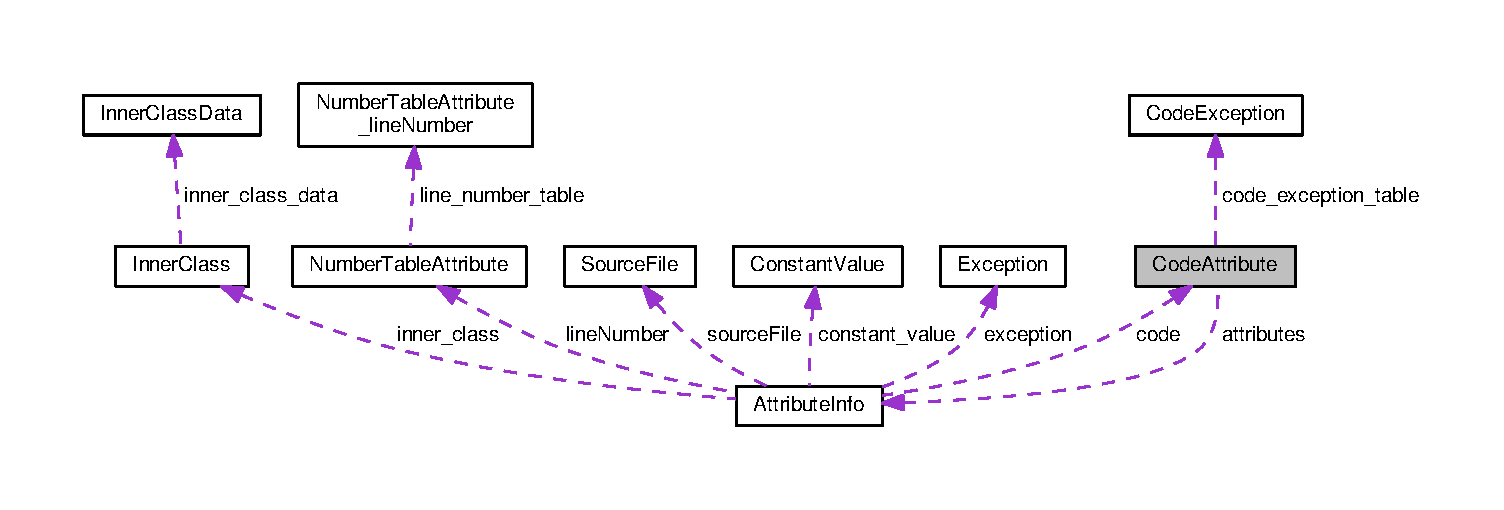
\includegraphics[width=350pt]{class_code_attribute__coll__graph}
\end{center}
\end{figure}
\subsection*{Componentes}
\begin{DoxyCompactItemize}
\item 
class \hyperlink{class_code_attribute_1_1print}{print}
\begin{DoxyCompactList}\small\item\em Print dos atributos dos methods;. \end{DoxyCompactList}\item 
class \hyperlink{class_code_attribute_1_1read}{read}
\begin{DoxyCompactList}\small\item\em Leitor dos atributos dos methods;. \end{DoxyCompactList}\item 
class \hyperlink{class_code_attribute_1_1~_code_attribute}{$\sim$\+Code\+Attribute}
\begin{DoxyCompactList}\small\item\em Destrutor \hyperlink{class_code_attribute}{Code\+Attribute}. \end{DoxyCompactList}\end{DoxyCompactItemize}
\subsection*{Membros públicos}
\begin{DoxyCompactItemize}
\item 
\hyperlink{class_code_attribute_a4053ae31518d02d7b374284b05217a7b}{$\sim$\+Code\+Attribute} ()
\item 
void \hyperlink{class_code_attribute_ae5c7888c59b2a2990798c597c014a2ac}{read} (F\+I\+LE $\ast$, std\+::vector$<$ \hyperlink{class_cp_info}{Cp\+Info} $\ast$ $>$)
\item 
void \hyperlink{class_code_attribute_a380eb04a01b0a0db351cf74443067ba4}{print} (std\+::vector$<$ \hyperlink{class_cp_info}{Cp\+Info} $\ast$ $>$)
\end{DoxyCompactItemize}
\subsection*{Atributos Públicos}
\begin{DoxyCompactItemize}
\item 
uint16\+\_\+t \hyperlink{class_code_attribute_aa98def02b93e04d31b8e5c1cc12458f8}{max\+\_\+stacks}
\item 
uint16\+\_\+t \hyperlink{class_code_attribute_a5e2d72942cf05feb8a512fcae6c3b2f3}{max\+\_\+locals}
\item 
uint32\+\_\+t \hyperlink{class_code_attribute_a78ee2a78d9310a51b91d07b39813bc73}{code\+\_\+length}
\item 
uint8\+\_\+t $\ast$ \hyperlink{class_code_attribute_a95d8e9c3e0b93220defcbc9852ec6c27}{code}
\item 
uint16\+\_\+t \hyperlink{class_code_attribute_a2ccde57be0af451e0bf4dcae05e67cc7}{exception\+\_\+table\+\_\+length}
\item 
\hyperlink{class_code_exception}{Code\+Exception} $\ast$ \hyperlink{class_code_attribute_abfc09247d38ec6d587a9059db38103ae}{code\+\_\+exception\+\_\+table}
\item 
uint16\+\_\+t \hyperlink{class_code_attribute_a7a5c471692a3376b19d7b55b034b7c45}{attributes\+\_\+count}
\item 
\hyperlink{class_attribute_info}{Attribute\+Info} $\ast$ \hyperlink{class_code_attribute_a99297a4945c876dd5615d84986043c21}{attributes}
\end{DoxyCompactItemize}


\subsection{Descrição detalhada}
classe Atributos que consiste em max\+\_\+stacks, max\+\_\+locals, code\+\_\+length(uint32), ponteiro para code(uint8), exception\+\_\+table\+\_\+length, attribute\+\_\+count e attributes -\/ restante uint16; Além contém métodos como destrutor, leitor e print 

\subsection{Documentação dos Construtores \& Destrutor}
\index{Code\+Attribute@{Code\+Attribute}!````~Code\+Attribute@{$\sim$\+Code\+Attribute}}
\index{````~Code\+Attribute@{$\sim$\+Code\+Attribute}!Code\+Attribute@{Code\+Attribute}}
\subsubsection[{\texorpdfstring{$\sim$\+Code\+Attribute()}{~CodeAttribute()}}]{\setlength{\rightskip}{0pt plus 5cm}{\bf Code\+Attribute\+::$\sim$\+Code\+Attribute} (
\begin{DoxyParamCaption}
{}
\end{DoxyParamCaption}
)}\hypertarget{class_code_attribute_a4053ae31518d02d7b374284b05217a7b}{}\label{class_code_attribute_a4053ae31518d02d7b374284b05217a7b}


\subsection{Documentação dos métodos}
\index{Code\+Attribute@{Code\+Attribute}!print@{print}}
\index{print@{print}!Code\+Attribute@{Code\+Attribute}}
\subsubsection[{\texorpdfstring{print(std\+::vector$<$ Cp\+Info $\ast$ $>$)}{print(std::vector< CpInfo * >)}}]{\setlength{\rightskip}{0pt plus 5cm}void {\bf Code\+Attribute\+::print} (
\begin{DoxyParamCaption}
\item[{std\+::vector$<$ {\bf Cp\+Info} $\ast$ $>$}]{true\+Cp\+Info}
\end{DoxyParamCaption}
)}\hypertarget{class_code_attribute_a380eb04a01b0a0db351cf74443067ba4}{}\label{class_code_attribute_a380eb04a01b0a0db351cf74443067ba4}


Grafo de chamadas desta função\+:
\nopagebreak
\begin{figure}[H]
\begin{center}
\leavevmode
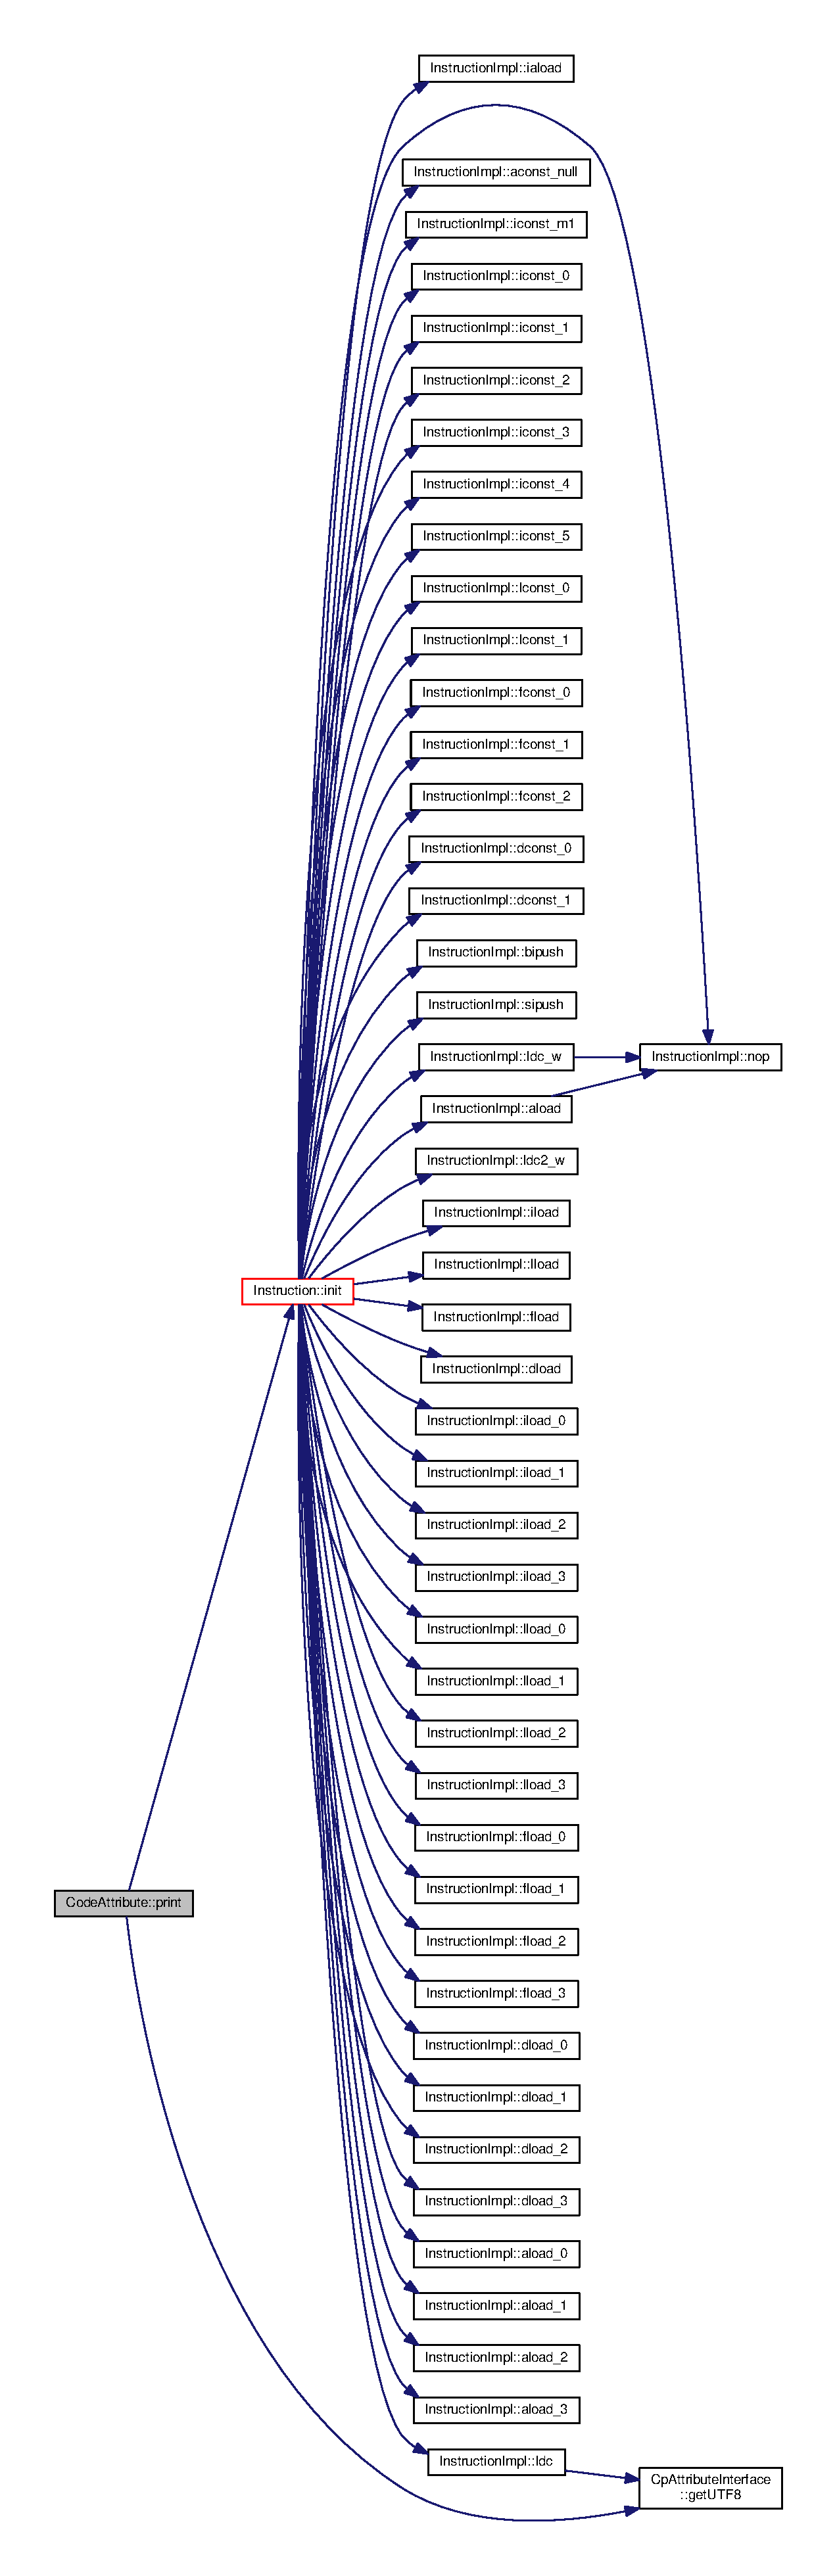
\includegraphics[height=550pt]{class_code_attribute_a380eb04a01b0a0db351cf74443067ba4_cgraph}
\end{center}
\end{figure}


\index{Code\+Attribute@{Code\+Attribute}!read@{read}}
\index{read@{read}!Code\+Attribute@{Code\+Attribute}}
\subsubsection[{\texorpdfstring{read(\+F\+I\+L\+E $\ast$, std\+::vector$<$ Cp\+Info $\ast$ $>$)}{read(FILE *, std::vector< CpInfo * >)}}]{\setlength{\rightskip}{0pt plus 5cm}void {\bf Code\+Attribute\+::read} (
\begin{DoxyParamCaption}
\item[{F\+I\+LE $\ast$}]{fp, }
\item[{std\+::vector$<$ {\bf Cp\+Info} $\ast$ $>$}]{true\+Cp\+Info}
\end{DoxyParamCaption}
)}\hypertarget{class_code_attribute_ae5c7888c59b2a2990798c597c014a2ac}{}\label{class_code_attribute_ae5c7888c59b2a2990798c597c014a2ac}


Grafo de chamadas desta função\+:
\nopagebreak
\begin{figure}[H]
\begin{center}
\leavevmode
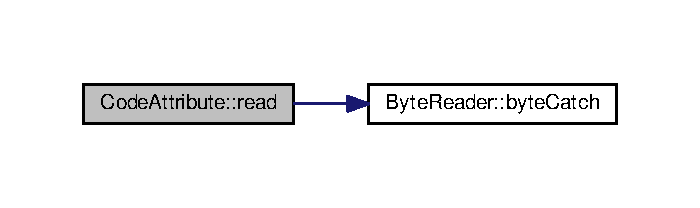
\includegraphics[width=336pt]{class_code_attribute_ae5c7888c59b2a2990798c597c014a2ac_cgraph}
\end{center}
\end{figure}




\subsection{Documentação dos dados membro}
\index{Code\+Attribute@{Code\+Attribute}!attributes@{attributes}}
\index{attributes@{attributes}!Code\+Attribute@{Code\+Attribute}}
\subsubsection[{\texorpdfstring{attributes}{attributes}}]{\setlength{\rightskip}{0pt plus 5cm}{\bf Attribute\+Info}$\ast$ Code\+Attribute\+::attributes}\hypertarget{class_code_attribute_a99297a4945c876dd5615d84986043c21}{}\label{class_code_attribute_a99297a4945c876dd5615d84986043c21}
\index{Code\+Attribute@{Code\+Attribute}!attributes\+\_\+count@{attributes\+\_\+count}}
\index{attributes\+\_\+count@{attributes\+\_\+count}!Code\+Attribute@{Code\+Attribute}}
\subsubsection[{\texorpdfstring{attributes\+\_\+count}{attributes_count}}]{\setlength{\rightskip}{0pt plus 5cm}uint16\+\_\+t Code\+Attribute\+::attributes\+\_\+count}\hypertarget{class_code_attribute_a7a5c471692a3376b19d7b55b034b7c45}{}\label{class_code_attribute_a7a5c471692a3376b19d7b55b034b7c45}
\index{Code\+Attribute@{Code\+Attribute}!code@{code}}
\index{code@{code}!Code\+Attribute@{Code\+Attribute}}
\subsubsection[{\texorpdfstring{code}{code}}]{\setlength{\rightskip}{0pt plus 5cm}uint8\+\_\+t$\ast$ Code\+Attribute\+::code}\hypertarget{class_code_attribute_a95d8e9c3e0b93220defcbc9852ec6c27}{}\label{class_code_attribute_a95d8e9c3e0b93220defcbc9852ec6c27}
\index{Code\+Attribute@{Code\+Attribute}!code\+\_\+exception\+\_\+table@{code\+\_\+exception\+\_\+table}}
\index{code\+\_\+exception\+\_\+table@{code\+\_\+exception\+\_\+table}!Code\+Attribute@{Code\+Attribute}}
\subsubsection[{\texorpdfstring{code\+\_\+exception\+\_\+table}{code_exception_table}}]{\setlength{\rightskip}{0pt plus 5cm}{\bf Code\+Exception}$\ast$ Code\+Attribute\+::code\+\_\+exception\+\_\+table}\hypertarget{class_code_attribute_abfc09247d38ec6d587a9059db38103ae}{}\label{class_code_attribute_abfc09247d38ec6d587a9059db38103ae}
\index{Code\+Attribute@{Code\+Attribute}!code\+\_\+length@{code\+\_\+length}}
\index{code\+\_\+length@{code\+\_\+length}!Code\+Attribute@{Code\+Attribute}}
\subsubsection[{\texorpdfstring{code\+\_\+length}{code_length}}]{\setlength{\rightskip}{0pt plus 5cm}uint32\+\_\+t Code\+Attribute\+::code\+\_\+length}\hypertarget{class_code_attribute_a78ee2a78d9310a51b91d07b39813bc73}{}\label{class_code_attribute_a78ee2a78d9310a51b91d07b39813bc73}
\index{Code\+Attribute@{Code\+Attribute}!exception\+\_\+table\+\_\+length@{exception\+\_\+table\+\_\+length}}
\index{exception\+\_\+table\+\_\+length@{exception\+\_\+table\+\_\+length}!Code\+Attribute@{Code\+Attribute}}
\subsubsection[{\texorpdfstring{exception\+\_\+table\+\_\+length}{exception_table_length}}]{\setlength{\rightskip}{0pt plus 5cm}uint16\+\_\+t Code\+Attribute\+::exception\+\_\+table\+\_\+length}\hypertarget{class_code_attribute_a2ccde57be0af451e0bf4dcae05e67cc7}{}\label{class_code_attribute_a2ccde57be0af451e0bf4dcae05e67cc7}
\index{Code\+Attribute@{Code\+Attribute}!max\+\_\+locals@{max\+\_\+locals}}
\index{max\+\_\+locals@{max\+\_\+locals}!Code\+Attribute@{Code\+Attribute}}
\subsubsection[{\texorpdfstring{max\+\_\+locals}{max_locals}}]{\setlength{\rightskip}{0pt plus 5cm}uint16\+\_\+t Code\+Attribute\+::max\+\_\+locals}\hypertarget{class_code_attribute_a5e2d72942cf05feb8a512fcae6c3b2f3}{}\label{class_code_attribute_a5e2d72942cf05feb8a512fcae6c3b2f3}
\index{Code\+Attribute@{Code\+Attribute}!max\+\_\+stacks@{max\+\_\+stacks}}
\index{max\+\_\+stacks@{max\+\_\+stacks}!Code\+Attribute@{Code\+Attribute}}
\subsubsection[{\texorpdfstring{max\+\_\+stacks}{max_stacks}}]{\setlength{\rightskip}{0pt plus 5cm}uint16\+\_\+t Code\+Attribute\+::max\+\_\+stacks}\hypertarget{class_code_attribute_aa98def02b93e04d31b8e5c1cc12458f8}{}\label{class_code_attribute_aa98def02b93e04d31b8e5c1cc12458f8}


A documentação para esta classe foi gerada a partir dos seguintes ficheiros\+:\begin{DoxyCompactItemize}
\item 
\hyperlink{_attribute_info_8hpp}{Attribute\+Info.\+hpp}\item 
\hyperlink{_attribute_info_8cpp}{Attribute\+Info.\+cpp}\end{DoxyCompactItemize}

\hypertarget{class_code_exception}{}\section{Code\+Exception Class Reference}
\label{class_code_exception}\index{Code\+Exception@{Code\+Exception}}


classe contém start\+\_\+pc, end\+\_\+pc, handler\+\_\+pc e catch\+\_\+type -\/ todos uint16;  




{\ttfamily \#include $<$Attribute\+Info.\+hpp$>$}

\subsection*{Public Attributes}
\begin{DoxyCompactItemize}
\item 
uint16\+\_\+t \hyperlink{class_code_exception_a18754b054d8331acbad758612698e599}{start\+\_\+pc}
\item 
uint16\+\_\+t \hyperlink{class_code_exception_a357306bca81fcf2e7bc9dfcedc9c4f96}{end\+\_\+pc}
\item 
uint16\+\_\+t \hyperlink{class_code_exception_a8c66a2462bd2668d7824e7f3745385d6}{handler\+\_\+pc}
\item 
uint16\+\_\+t \hyperlink{class_code_exception_a0b2110e6c93d442c66cf10563920537c}{catch\+\_\+type}
\end{DoxyCompactItemize}


\subsection{Detailed Description}
classe contém start\+\_\+pc, end\+\_\+pc, handler\+\_\+pc e catch\+\_\+type -\/ todos uint16; 

\subsection{Member Data Documentation}
\index{Code\+Exception@{Code\+Exception}!catch\+\_\+type@{catch\+\_\+type}}
\index{catch\+\_\+type@{catch\+\_\+type}!Code\+Exception@{Code\+Exception}}
\subsubsection[{\texorpdfstring{catch\+\_\+type}{catch_type}}]{\setlength{\rightskip}{0pt plus 5cm}uint16\+\_\+t Code\+Exception\+::catch\+\_\+type}\hypertarget{class_code_exception_a0b2110e6c93d442c66cf10563920537c}{}\label{class_code_exception_a0b2110e6c93d442c66cf10563920537c}
\index{Code\+Exception@{Code\+Exception}!end\+\_\+pc@{end\+\_\+pc}}
\index{end\+\_\+pc@{end\+\_\+pc}!Code\+Exception@{Code\+Exception}}
\subsubsection[{\texorpdfstring{end\+\_\+pc}{end_pc}}]{\setlength{\rightskip}{0pt plus 5cm}uint16\+\_\+t Code\+Exception\+::end\+\_\+pc}\hypertarget{class_code_exception_a357306bca81fcf2e7bc9dfcedc9c4f96}{}\label{class_code_exception_a357306bca81fcf2e7bc9dfcedc9c4f96}
\index{Code\+Exception@{Code\+Exception}!handler\+\_\+pc@{handler\+\_\+pc}}
\index{handler\+\_\+pc@{handler\+\_\+pc}!Code\+Exception@{Code\+Exception}}
\subsubsection[{\texorpdfstring{handler\+\_\+pc}{handler_pc}}]{\setlength{\rightskip}{0pt plus 5cm}uint16\+\_\+t Code\+Exception\+::handler\+\_\+pc}\hypertarget{class_code_exception_a8c66a2462bd2668d7824e7f3745385d6}{}\label{class_code_exception_a8c66a2462bd2668d7824e7f3745385d6}
\index{Code\+Exception@{Code\+Exception}!start\+\_\+pc@{start\+\_\+pc}}
\index{start\+\_\+pc@{start\+\_\+pc}!Code\+Exception@{Code\+Exception}}
\subsubsection[{\texorpdfstring{start\+\_\+pc}{start_pc}}]{\setlength{\rightskip}{0pt plus 5cm}uint16\+\_\+t Code\+Exception\+::start\+\_\+pc}\hypertarget{class_code_exception_a18754b054d8331acbad758612698e599}{}\label{class_code_exception_a18754b054d8331acbad758612698e599}


The documentation for this class was generated from the following file\+:\begin{DoxyCompactItemize}
\item 
\hyperlink{_attribute_info_8hpp}{Attribute\+Info.\+hpp}\end{DoxyCompactItemize}

\hypertarget{class_constant_value}{}\section{Constant\+Value Class Reference}
\label{class_constant_value}\index{Constant\+Value@{Constant\+Value}}


classe contém Além contém métodos como destrutor, leitor e print  




{\ttfamily \#include $<$Attribute\+Info.\+hpp$>$}

\subsection*{Classes}
\begin{DoxyCompactItemize}
\item 
class \hyperlink{class_constant_value_1_1print}{print}
\begin{DoxyCompactList}\small\item\em print dos valores das constantes; \end{DoxyCompactList}\item 
class \hyperlink{class_constant_value_1_1read}{read}
\begin{DoxyCompactList}\small\item\em Leitor de constantes;. \end{DoxyCompactList}\end{DoxyCompactItemize}
\subsection*{Public Member Functions}
\begin{DoxyCompactItemize}
\item 
void \hyperlink{class_constant_value_aee71ff590a730276c8da00dbdee74ecf}{read} (F\+I\+LE $\ast$)
\item 
void \hyperlink{class_constant_value_a99dd9b4165766a0347e126c580fa93d0}{print} (std\+::vector$<$ \hyperlink{class_cp_info}{Cp\+Info} $\ast$ $>$)
\end{DoxyCompactItemize}
\subsection*{Public Attributes}
\begin{DoxyCompactItemize}
\item 
uint16\+\_\+t \hyperlink{class_constant_value_aaa51c41fc17e11c759e2d0dccbf178e8}{constvalue\+\_\+index}
\end{DoxyCompactItemize}


\subsection{Detailed Description}
classe contém Além contém métodos como destrutor, leitor e print 

\subsection{Member Function Documentation}
\index{Constant\+Value@{Constant\+Value}!print@{print}}
\index{print@{print}!Constant\+Value@{Constant\+Value}}
\subsubsection[{\texorpdfstring{print(std\+::vector$<$ Cp\+Info $\ast$ $>$)}{print(std::vector< CpInfo * >)}}]{\setlength{\rightskip}{0pt plus 5cm}void {\bf Constant\+Value\+::print} (
\begin{DoxyParamCaption}
\item[{std\+::vector$<$ {\bf Cp\+Info} $\ast$ $>$}]{true\+Cp\+Info}
\end{DoxyParamCaption}
)}\hypertarget{class_constant_value_a99dd9b4165766a0347e126c580fa93d0}{}\label{class_constant_value_a99dd9b4165766a0347e126c580fa93d0}


Here is the call graph for this function\+:
% FIG 0


\index{Constant\+Value@{Constant\+Value}!read@{read}}
\index{read@{read}!Constant\+Value@{Constant\+Value}}
\subsubsection[{\texorpdfstring{read(\+F\+I\+L\+E $\ast$)}{read(FILE *)}}]{\setlength{\rightskip}{0pt plus 5cm}void {\bf Constant\+Value\+::read} (
\begin{DoxyParamCaption}
\item[{F\+I\+LE $\ast$}]{fp}
\end{DoxyParamCaption}
)}\hypertarget{class_constant_value_aee71ff590a730276c8da00dbdee74ecf}{}\label{class_constant_value_aee71ff590a730276c8da00dbdee74ecf}


Here is the call graph for this function\+:
% FIG 1




\subsection{Member Data Documentation}
\index{Constant\+Value@{Constant\+Value}!constvalue\+\_\+index@{constvalue\+\_\+index}}
\index{constvalue\+\_\+index@{constvalue\+\_\+index}!Constant\+Value@{Constant\+Value}}
\subsubsection[{\texorpdfstring{constvalue\+\_\+index}{constvalue_index}}]{\setlength{\rightskip}{0pt plus 5cm}uint16\+\_\+t Constant\+Value\+::constvalue\+\_\+index}\hypertarget{class_constant_value_aaa51c41fc17e11c759e2d0dccbf178e8}{}\label{class_constant_value_aaa51c41fc17e11c759e2d0dccbf178e8}


The documentation for this class was generated from the following files\+:\begin{DoxyCompactItemize}
\item 
\hyperlink{_attribute_info_8hpp}{Attribute\+Info.\+hpp}\item 
\hyperlink{_attribute_info_8cpp}{Attribute\+Info.\+cpp}\end{DoxyCompactItemize}

\hypertarget{struct_cp_attribute_interface}{}\section{Referência à classe Cp\+Attribute\+Interface}
\label{struct_cp_attribute_interface}\index{Cp\+Attribute\+Interface@{Cp\+Attribute\+Interface}}


Declarações da interface entre Constant\+Pool e \hyperlink{class_attribute_info}{Attribute\+Info} para traduzir as strings U\+T\+F8.  




{\ttfamily \#include $<$Cp\+Attribute\+Interface.\+hpp$>$}

\subsection*{Componentes}
\begin{DoxyCompactItemize}
\item 
class \hyperlink{class_cp_attribute_interface_1_1get_u_t_f8}{get\+U\+T\+F8}
\begin{DoxyCompactList}\small\item\em Função que realiza buscas recursivas dentro do \hyperlink{class_cp_info}{Cp\+Info} de um bytecode. \end{DoxyCompactList}\end{DoxyCompactItemize}
\subsection*{Membros públicos}
\begin{DoxyCompactItemize}
\item 
std\+::string \hyperlink{struct_cp_attribute_interface_a99cabbc15a0af5273a6d324dfbc78f41}{get\+U\+T\+F8} (std\+::vector$<$ \hyperlink{class_cp_info}{Cp\+Info} $\ast$ $>$, uint16\+\_\+t)
\end{DoxyCompactItemize}


\subsection{Descrição detalhada}
Declarações da interface entre Constant\+Pool e \hyperlink{class_attribute_info}{Attribute\+Info} para traduzir as strings U\+T\+F8. 

\subsection{Documentação dos métodos}
\index{Cp\+Attribute\+Interface@{Cp\+Attribute\+Interface}!get\+U\+T\+F8@{get\+U\+T\+F8}}
\index{get\+U\+T\+F8@{get\+U\+T\+F8}!Cp\+Attribute\+Interface@{Cp\+Attribute\+Interface}}
\subsubsection[{\texorpdfstring{get\+U\+T\+F8(std\+::vector$<$ Cp\+Info $\ast$ $>$, uint16\+\_\+t)}{getUTF8(std::vector< CpInfo * >, uint16_t)}}]{\setlength{\rightskip}{0pt plus 5cm}std\+::string {\bf Cp\+Attribute\+Interface\+::get\+U\+T\+F8} (
\begin{DoxyParamCaption}
\item[{std\+::vector$<$ {\bf Cp\+Info} $\ast$ $>$}]{alpha, }
\item[{uint16\+\_\+t}]{beta}
\end{DoxyParamCaption}
)}\hypertarget{struct_cp_attribute_interface_a99cabbc15a0af5273a6d324dfbc78f41}{}\label{struct_cp_attribute_interface_a99cabbc15a0af5273a6d324dfbc78f41}


Este é o diagrama das funções que utilizam esta função\+:
\nopagebreak
\begin{figure}[H]
\begin{center}
\leavevmode
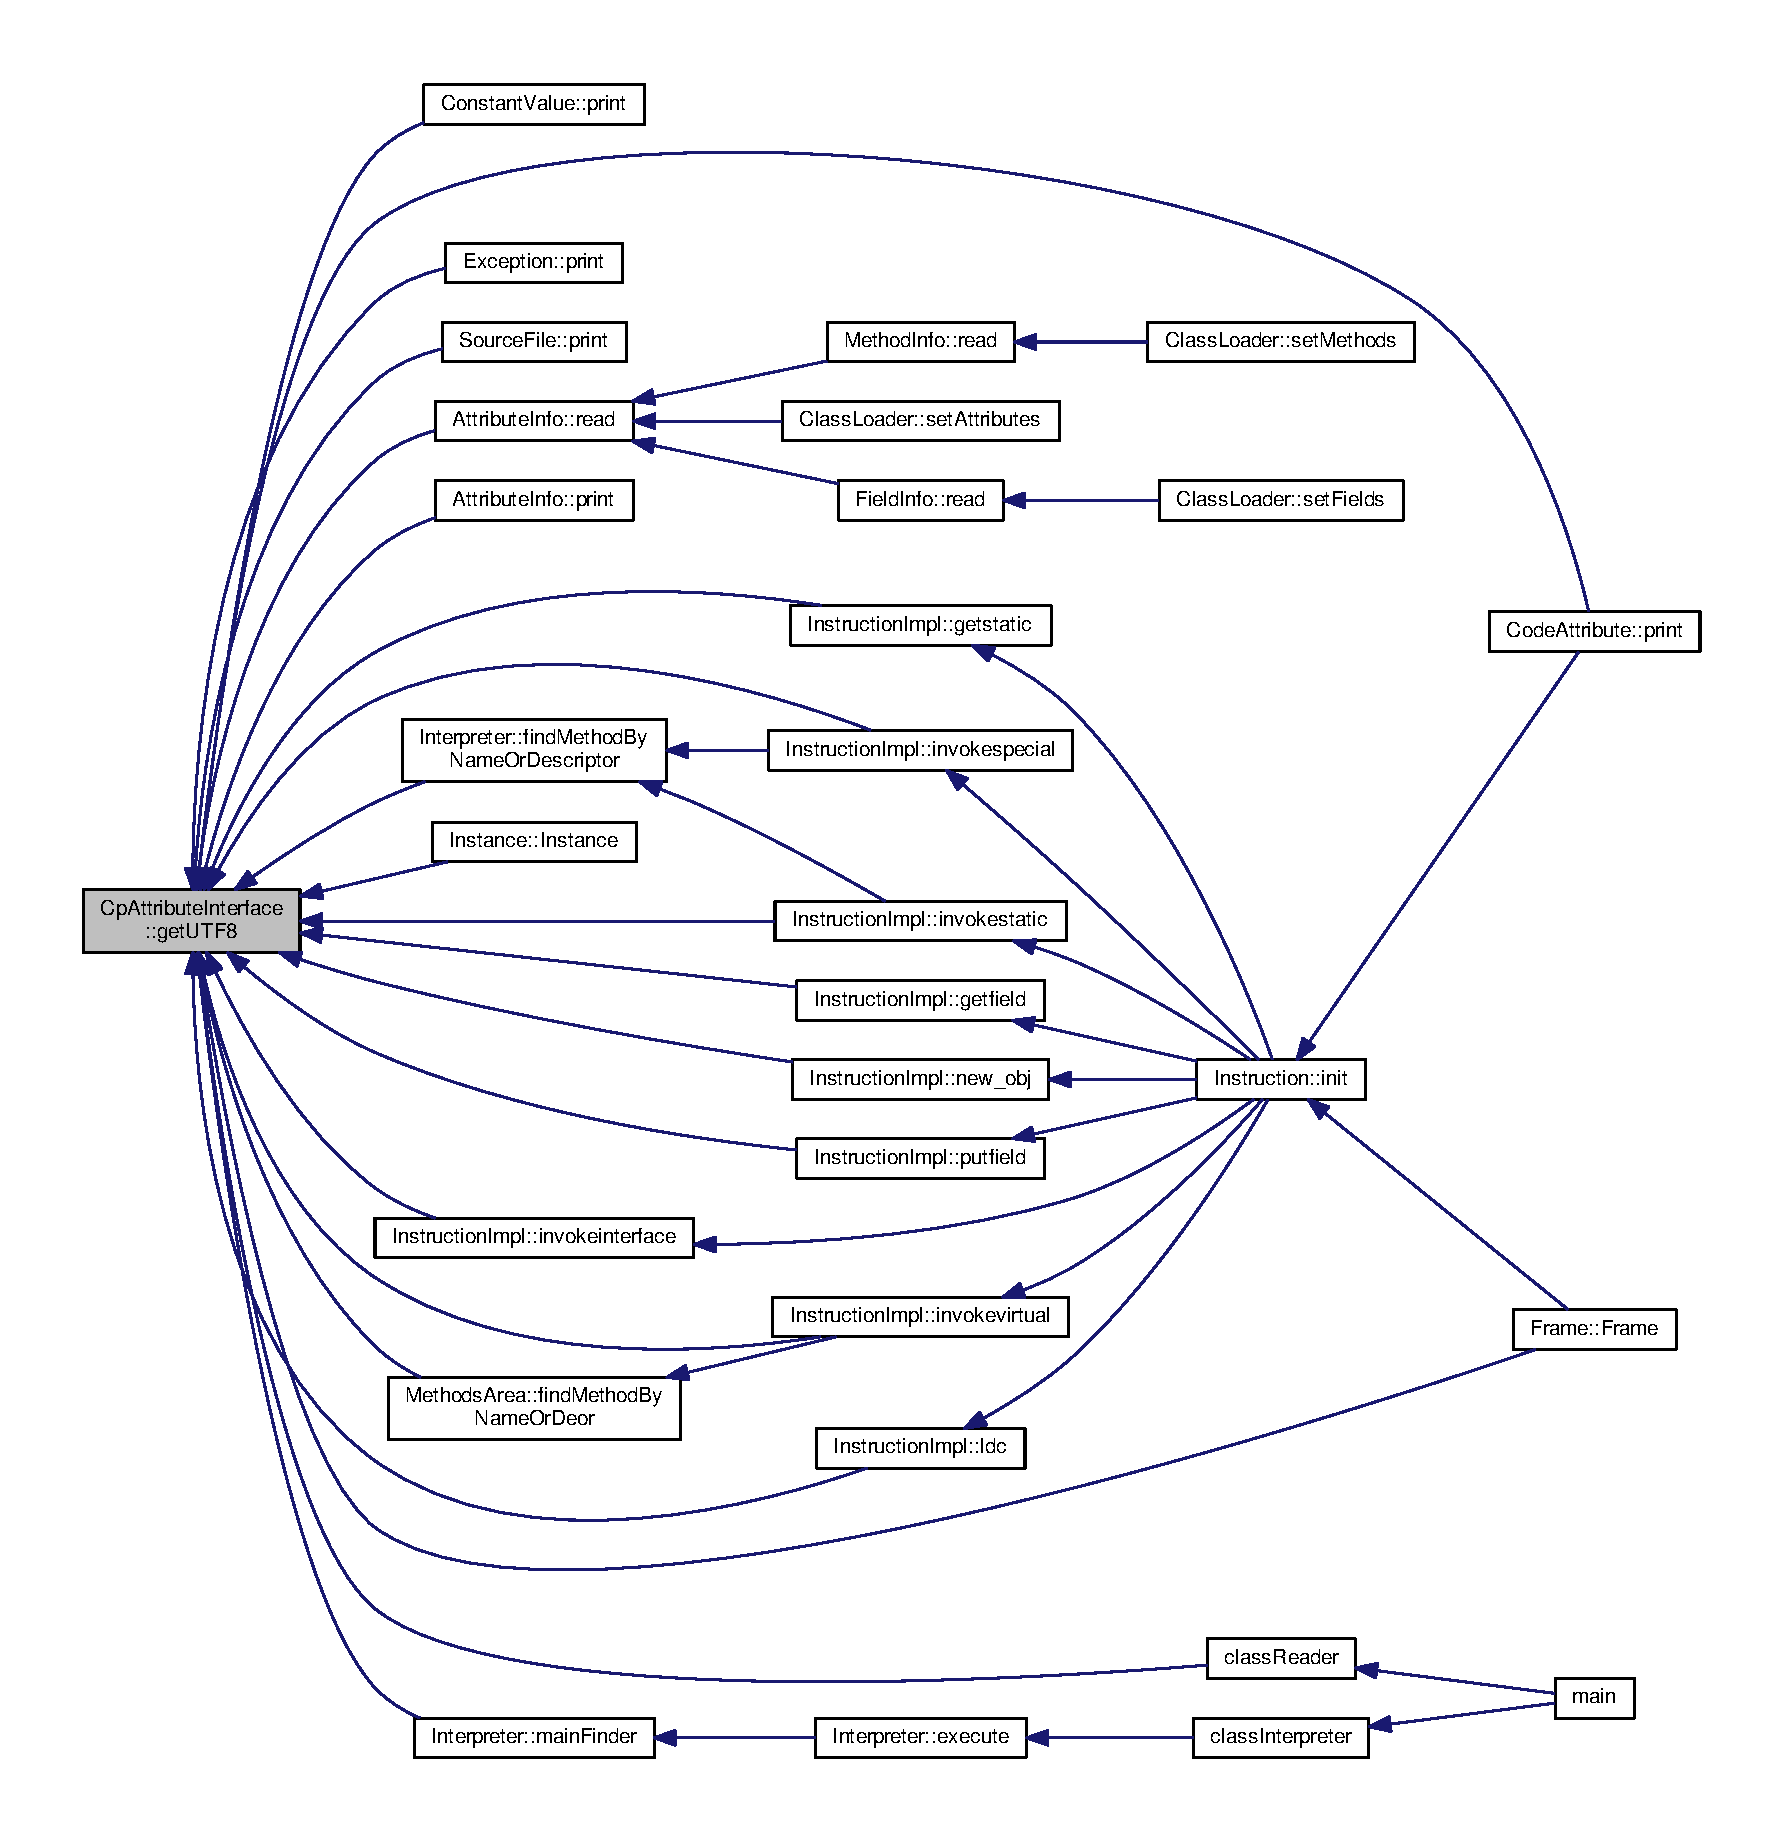
\includegraphics[width=350pt]{struct_cp_attribute_interface_a99cabbc15a0af5273a6d324dfbc78f41_icgraph}
\end{center}
\end{figure}




A documentação para esta classe foi gerada a partir dos seguintes ficheiros\+:\begin{DoxyCompactItemize}
\item 
\hyperlink{_cp_attribute_interface_8hpp}{Cp\+Attribute\+Interface.\+hpp}\item 
\hyperlink{_cp_attribute_interface_8cpp}{Cp\+Attribute\+Interface.\+cpp}\end{DoxyCompactItemize}

\hypertarget{class_cp_info}{}\section{Referência à classe Cp\+Info}
\label{class_cp_info}\index{Cp\+Info@{Cp\+Info}}


Classe contém tag(uint8) e union que será um tipo diferente dependendo de qual tag que será passada;.  




{\ttfamily \#include $<$Cp\+Info.\+hpp$>$}

\subsection*{Componentes}
\begin{DoxyCompactItemize}
\item 
class \hyperlink{class_cp_info_1_1read}{read}
\begin{DoxyCompactList}\small\item\em realiza o set inicial das variáveis a partir do \end{DoxyCompactList}\item 
class \hyperlink{class_cp_info_1_1~_cp_info}{$\sim$\+Cp\+Info}
\begin{DoxyCompactList}\small\item\em Destrutor de \hyperlink{class_cp_info}{Cp\+Info}, desaloca o que foi alocado. \end{DoxyCompactList}\end{DoxyCompactItemize}
\subsection*{Membros públicos}
\begin{DoxyCompactItemize}
\item 
\hyperlink{class_cp_info_a67ca1fe35f94943081010ec05cb7d464}{$\sim$\+Cp\+Info} ()
\item 
void \hyperlink{class_cp_info_ab8c89df973cc40b407e0cdd4911923f1}{read} (F\+I\+LE $\ast$fp)
\end{DoxyCompactItemize}
\subsection*{Atributos Públicos}
\begin{DoxyCompactItemize}
\item 
uint8\+\_\+t \hyperlink{class_cp_info_ac20d96c33f871bde2e903708a215a2dc}{tag}
\item 
\begin{tabbing}
xx\=xx\=xx\=xx\=xx\=xx\=xx\=xx\=xx\=\kill
union \{\\
\>struct \{\\
\>\>uint16\_t \hyperlink{class_cp_info_a8337463c52221eaead88f232ded768a7}{name\_index}\\
\>\} \hyperlink{class_cp_info_a8e42eb58082f93477cecc14d96c50689}{Class}\\
\>struct \{\\
\>\>uint16\_t \hyperlink{class_cp_info_abde12c60f120eb082631fd0554fbe2f3}{class\_index}\\
\>\>uint16\_t \hyperlink{class_cp_info_a3007bcc993f983836f419c3d8f8cb835}{name\_and\_type\_index}\\
\>\} \hyperlink{class_cp_info_a9f594a9412a1d3bfc086efc127fb528a}{Fieldref}\\
\>struct \{\\
\>\>uint16\_t \hyperlink{class_cp_info_abde12c60f120eb082631fd0554fbe2f3}{class\_index}\\
\>\>uint16\_t \hyperlink{class_cp_info_a3007bcc993f983836f419c3d8f8cb835}{name\_and\_type\_index}\\
\>\} \hyperlink{class_cp_info_ac86976e076271c25fb990d34cbf93eb1}{Methodref}\\
\>struct \{\\
\>\>uint16\_t \hyperlink{class_cp_info_abde12c60f120eb082631fd0554fbe2f3}{class\_index}\\
\>\>uint16\_t \hyperlink{class_cp_info_a3007bcc993f983836f419c3d8f8cb835}{name\_and\_type\_index}\\
\>\} \hyperlink{class_cp_info_ad489482113b9905436258696227b9d21}{InterfaceMethodref}\\
\>struct \{\\
\>\>uint16\_t \hyperlink{class_cp_info_a4b2f7aa4ac461ac4d860d566c5e3323e}{string\_index}\\
\>\} \hyperlink{class_cp_info_a9e47b825b6e22ad57a9b78cf430cd6bc}{String}\\
\>struct \{\\
\>\>uint32\_t \hyperlink{class_cp_info_aff3858879ad5feb452a5fc0504e99c1b}{bytes}\\
\>\} \hyperlink{class_cp_info_a873ae1d00d8658008893f3397ad3535b}{Integer}\\
\>struct \{\\
\>\>uint32\_t \hyperlink{class_cp_info_aff3858879ad5feb452a5fc0504e99c1b}{bytes}\\
\>\} \hyperlink{class_cp_info_a8dd439e3f1f235a10abf65991a89c0e0}{Float}\\
\>struct \{\\
\>\>uint32\_t \hyperlink{class_cp_info_a4ddca9fe1db833914bba6fccab4a4966}{high\_bytes}\\
\>\>uint32\_t \hyperlink{class_cp_info_a361c4ed0f0ba7c54dec3469e1e2b67ce}{low\_bytes}\\
\>\} \hyperlink{class_cp_info_a57c0bb8dfad66c7c75c552ab6ca45563}{Long}\\
\>struct \{\\
\>\>uint32\_t \hyperlink{class_cp_info_a4ddca9fe1db833914bba6fccab4a4966}{high\_bytes}\\
\>\>uint32\_t \hyperlink{class_cp_info_a361c4ed0f0ba7c54dec3469e1e2b67ce}{low\_bytes}\\
\>\} \hyperlink{class_cp_info_a8d321b2411c3720d3009722182a2fbd5}{Double}\\
\>struct \{\\
\>\>uint16\_t \hyperlink{class_cp_info_a8337463c52221eaead88f232ded768a7}{name\_index}\\
\>\>uint16\_t \hyperlink{class_cp_info_a1e5f422fa619e06a2deb2728be023381}{descriptor\_index}\\
\>\} \hyperlink{class_cp_info_af8ab428cfd1348391c7d3b26d94d6567}{NameAndType}\\
\>struct \{\\
\>\>uint16\_t \hyperlink{class_cp_info_a8876751cacc7818d9748366a35ef85f7}{length}\\
\>\>uint8\_t $\ast$ \hyperlink{class_cp_info_acdf9242daedb1b37c82f24e6665edb10}{bytes}\\
\>\} \hyperlink{class_cp_info_a1959c604c24ea0a8c2ab8a4f3094f3e0}{UTF8}\\
\}; \\

\end{tabbing}\end{DoxyCompactItemize}


\subsection{Descrição detalhada}
Classe contém tag(uint8) e union que será um tipo diferente dependendo de qual tag que será passada;. 

\subsection{Documentação dos Construtores \& Destrutor}
\index{Cp\+Info@{Cp\+Info}!````~Cp\+Info@{$\sim$\+Cp\+Info}}
\index{````~Cp\+Info@{$\sim$\+Cp\+Info}!Cp\+Info@{Cp\+Info}}
\subsubsection[{\texorpdfstring{$\sim$\+Cp\+Info()}{~CpInfo()}}]{\setlength{\rightskip}{0pt plus 5cm}{\bf Cp\+Info\+::$\sim$\+Cp\+Info} (
\begin{DoxyParamCaption}
{}
\end{DoxyParamCaption}
)}\hypertarget{class_cp_info_a67ca1fe35f94943081010ec05cb7d464}{}\label{class_cp_info_a67ca1fe35f94943081010ec05cb7d464}


\subsection{Documentação dos métodos}
\index{Cp\+Info@{Cp\+Info}!read@{read}}
\index{read@{read}!Cp\+Info@{Cp\+Info}}
\subsubsection[{\texorpdfstring{read(\+F\+I\+L\+E $\ast$fp)}{read(FILE *fp)}}]{\setlength{\rightskip}{0pt plus 5cm}void {\bf Cp\+Info\+::read} (
\begin{DoxyParamCaption}
\item[{F\+I\+LE $\ast$}]{fp}
\end{DoxyParamCaption}
)}\hypertarget{class_cp_info_ab8c89df973cc40b407e0cdd4911923f1}{}\label{class_cp_info_ab8c89df973cc40b407e0cdd4911923f1}
A alocação via calloc é feita aqui com o entuito de settar os valores como 0 inicialmente. Alocala-\/se um total de lenght+1 posições para que ao final possa se inserir o caractere \textquotesingle{}\textbackslash{}0\textquotesingle{} sem acessar uma região de memória não garantida para nosso programa.

Grafo de chamadas desta função\+:
\nopagebreak
\begin{figure}[H]
\begin{center}
\leavevmode
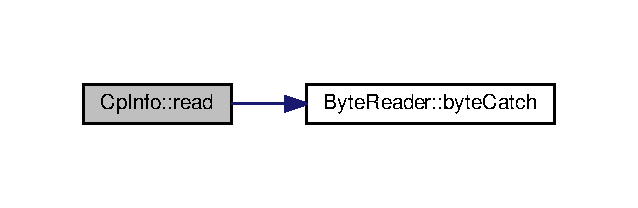
\includegraphics[width=306pt]{class_cp_info_ab8c89df973cc40b407e0cdd4911923f1_cgraph}
\end{center}
\end{figure}




Este é o diagrama das funções que utilizam esta função\+:
\nopagebreak
\begin{figure}[H]
\begin{center}
\leavevmode
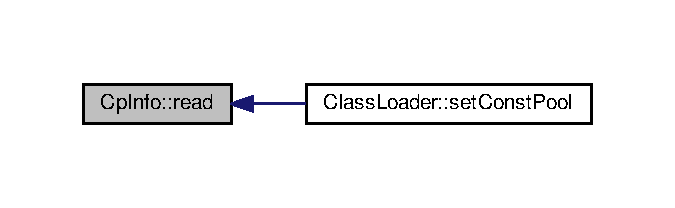
\includegraphics[width=324pt]{class_cp_info_ab8c89df973cc40b407e0cdd4911923f1_icgraph}
\end{center}
\end{figure}




\subsection{Documentação dos dados membro}
\subsubsection[{\texorpdfstring{"@3}{@3}}]{\setlength{\rightskip}{0pt plus 5cm}union \{ ... \} }\hypertarget{class_cp_info_ac48d2f19350cfd3fb1d0c6a6b1537803}{}\label{class_cp_info_ac48d2f19350cfd3fb1d0c6a6b1537803}
\index{Cp\+Info@{Cp\+Info}!bytes@{bytes}}
\index{bytes@{bytes}!Cp\+Info@{Cp\+Info}}
\subsubsection[{\texorpdfstring{bytes}{bytes}}]{\setlength{\rightskip}{0pt plus 5cm}uint32\+\_\+t Cp\+Info\+::bytes}\hypertarget{class_cp_info_aff3858879ad5feb452a5fc0504e99c1b}{}\label{class_cp_info_aff3858879ad5feb452a5fc0504e99c1b}
\index{Cp\+Info@{Cp\+Info}!bytes@{bytes}}
\index{bytes@{bytes}!Cp\+Info@{Cp\+Info}}
\subsubsection[{\texorpdfstring{bytes}{bytes}}]{\setlength{\rightskip}{0pt plus 5cm}uint8\+\_\+t$\ast$ Cp\+Info\+::bytes}\hypertarget{class_cp_info_acdf9242daedb1b37c82f24e6665edb10}{}\label{class_cp_info_acdf9242daedb1b37c82f24e6665edb10}
\index{Cp\+Info@{Cp\+Info}!Class@{Class}}
\index{Class@{Class}!Cp\+Info@{Cp\+Info}}
\subsubsection[{\texorpdfstring{Class}{Class}}]{\setlength{\rightskip}{0pt plus 5cm}struct \{ ... \}   Cp\+Info\+::\+Class}\hypertarget{class_cp_info_a8e42eb58082f93477cecc14d96c50689}{}\label{class_cp_info_a8e42eb58082f93477cecc14d96c50689}
\index{Cp\+Info@{Cp\+Info}!class\+\_\+index@{class\+\_\+index}}
\index{class\+\_\+index@{class\+\_\+index}!Cp\+Info@{Cp\+Info}}
\subsubsection[{\texorpdfstring{class\+\_\+index}{class_index}}]{\setlength{\rightskip}{0pt plus 5cm}uint16\+\_\+t Cp\+Info\+::class\+\_\+index}\hypertarget{class_cp_info_abde12c60f120eb082631fd0554fbe2f3}{}\label{class_cp_info_abde12c60f120eb082631fd0554fbe2f3}
\index{Cp\+Info@{Cp\+Info}!descriptor\+\_\+index@{descriptor\+\_\+index}}
\index{descriptor\+\_\+index@{descriptor\+\_\+index}!Cp\+Info@{Cp\+Info}}
\subsubsection[{\texorpdfstring{descriptor\+\_\+index}{descriptor_index}}]{\setlength{\rightskip}{0pt plus 5cm}uint16\+\_\+t Cp\+Info\+::descriptor\+\_\+index}\hypertarget{class_cp_info_a1e5f422fa619e06a2deb2728be023381}{}\label{class_cp_info_a1e5f422fa619e06a2deb2728be023381}
\index{Cp\+Info@{Cp\+Info}!Double@{Double}}
\index{Double@{Double}!Cp\+Info@{Cp\+Info}}
\subsubsection[{\texorpdfstring{Double}{Double}}]{\setlength{\rightskip}{0pt plus 5cm}struct \{ ... \}   Cp\+Info\+::\+Double}\hypertarget{class_cp_info_a8d321b2411c3720d3009722182a2fbd5}{}\label{class_cp_info_a8d321b2411c3720d3009722182a2fbd5}
\index{Cp\+Info@{Cp\+Info}!Fieldref@{Fieldref}}
\index{Fieldref@{Fieldref}!Cp\+Info@{Cp\+Info}}
\subsubsection[{\texorpdfstring{Fieldref}{Fieldref}}]{\setlength{\rightskip}{0pt plus 5cm}struct \{ ... \}   Cp\+Info\+::\+Fieldref}\hypertarget{class_cp_info_a9f594a9412a1d3bfc086efc127fb528a}{}\label{class_cp_info_a9f594a9412a1d3bfc086efc127fb528a}
\index{Cp\+Info@{Cp\+Info}!Float@{Float}}
\index{Float@{Float}!Cp\+Info@{Cp\+Info}}
\subsubsection[{\texorpdfstring{Float}{Float}}]{\setlength{\rightskip}{0pt plus 5cm}struct \{ ... \}   Cp\+Info\+::\+Float}\hypertarget{class_cp_info_a8dd439e3f1f235a10abf65991a89c0e0}{}\label{class_cp_info_a8dd439e3f1f235a10abf65991a89c0e0}
\index{Cp\+Info@{Cp\+Info}!high\+\_\+bytes@{high\+\_\+bytes}}
\index{high\+\_\+bytes@{high\+\_\+bytes}!Cp\+Info@{Cp\+Info}}
\subsubsection[{\texorpdfstring{high\+\_\+bytes}{high_bytes}}]{\setlength{\rightskip}{0pt plus 5cm}uint32\+\_\+t Cp\+Info\+::high\+\_\+bytes}\hypertarget{class_cp_info_a4ddca9fe1db833914bba6fccab4a4966}{}\label{class_cp_info_a4ddca9fe1db833914bba6fccab4a4966}
\index{Cp\+Info@{Cp\+Info}!Integer@{Integer}}
\index{Integer@{Integer}!Cp\+Info@{Cp\+Info}}
\subsubsection[{\texorpdfstring{Integer}{Integer}}]{\setlength{\rightskip}{0pt plus 5cm}struct \{ ... \}   Cp\+Info\+::\+Integer}\hypertarget{class_cp_info_a873ae1d00d8658008893f3397ad3535b}{}\label{class_cp_info_a873ae1d00d8658008893f3397ad3535b}
\index{Cp\+Info@{Cp\+Info}!Interface\+Methodref@{Interface\+Methodref}}
\index{Interface\+Methodref@{Interface\+Methodref}!Cp\+Info@{Cp\+Info}}
\subsubsection[{\texorpdfstring{Interface\+Methodref}{InterfaceMethodref}}]{\setlength{\rightskip}{0pt plus 5cm}struct \{ ... \}   Cp\+Info\+::\+Interface\+Methodref}\hypertarget{class_cp_info_ad489482113b9905436258696227b9d21}{}\label{class_cp_info_ad489482113b9905436258696227b9d21}
\index{Cp\+Info@{Cp\+Info}!length@{length}}
\index{length@{length}!Cp\+Info@{Cp\+Info}}
\subsubsection[{\texorpdfstring{length}{length}}]{\setlength{\rightskip}{0pt plus 5cm}uint16\+\_\+t Cp\+Info\+::length}\hypertarget{class_cp_info_a8876751cacc7818d9748366a35ef85f7}{}\label{class_cp_info_a8876751cacc7818d9748366a35ef85f7}
\index{Cp\+Info@{Cp\+Info}!Long@{Long}}
\index{Long@{Long}!Cp\+Info@{Cp\+Info}}
\subsubsection[{\texorpdfstring{Long}{Long}}]{\setlength{\rightskip}{0pt plus 5cm}struct \{ ... \}   Cp\+Info\+::\+Long}\hypertarget{class_cp_info_a57c0bb8dfad66c7c75c552ab6ca45563}{}\label{class_cp_info_a57c0bb8dfad66c7c75c552ab6ca45563}
\index{Cp\+Info@{Cp\+Info}!low\+\_\+bytes@{low\+\_\+bytes}}
\index{low\+\_\+bytes@{low\+\_\+bytes}!Cp\+Info@{Cp\+Info}}
\subsubsection[{\texorpdfstring{low\+\_\+bytes}{low_bytes}}]{\setlength{\rightskip}{0pt plus 5cm}uint32\+\_\+t Cp\+Info\+::low\+\_\+bytes}\hypertarget{class_cp_info_a361c4ed0f0ba7c54dec3469e1e2b67ce}{}\label{class_cp_info_a361c4ed0f0ba7c54dec3469e1e2b67ce}
\index{Cp\+Info@{Cp\+Info}!Methodref@{Methodref}}
\index{Methodref@{Methodref}!Cp\+Info@{Cp\+Info}}
\subsubsection[{\texorpdfstring{Methodref}{Methodref}}]{\setlength{\rightskip}{0pt plus 5cm}struct \{ ... \}   Cp\+Info\+::\+Methodref}\hypertarget{class_cp_info_ac86976e076271c25fb990d34cbf93eb1}{}\label{class_cp_info_ac86976e076271c25fb990d34cbf93eb1}
\index{Cp\+Info@{Cp\+Info}!name\+\_\+and\+\_\+type\+\_\+index@{name\+\_\+and\+\_\+type\+\_\+index}}
\index{name\+\_\+and\+\_\+type\+\_\+index@{name\+\_\+and\+\_\+type\+\_\+index}!Cp\+Info@{Cp\+Info}}
\subsubsection[{\texorpdfstring{name\+\_\+and\+\_\+type\+\_\+index}{name_and_type_index}}]{\setlength{\rightskip}{0pt plus 5cm}uint16\+\_\+t Cp\+Info\+::name\+\_\+and\+\_\+type\+\_\+index}\hypertarget{class_cp_info_a3007bcc993f983836f419c3d8f8cb835}{}\label{class_cp_info_a3007bcc993f983836f419c3d8f8cb835}
\index{Cp\+Info@{Cp\+Info}!name\+\_\+index@{name\+\_\+index}}
\index{name\+\_\+index@{name\+\_\+index}!Cp\+Info@{Cp\+Info}}
\subsubsection[{\texorpdfstring{name\+\_\+index}{name_index}}]{\setlength{\rightskip}{0pt plus 5cm}uint16\+\_\+t Cp\+Info\+::name\+\_\+index}\hypertarget{class_cp_info_a8337463c52221eaead88f232ded768a7}{}\label{class_cp_info_a8337463c52221eaead88f232ded768a7}
\index{Cp\+Info@{Cp\+Info}!Name\+And\+Type@{Name\+And\+Type}}
\index{Name\+And\+Type@{Name\+And\+Type}!Cp\+Info@{Cp\+Info}}
\subsubsection[{\texorpdfstring{Name\+And\+Type}{NameAndType}}]{\setlength{\rightskip}{0pt plus 5cm}struct \{ ... \}   Cp\+Info\+::\+Name\+And\+Type}\hypertarget{class_cp_info_af8ab428cfd1348391c7d3b26d94d6567}{}\label{class_cp_info_af8ab428cfd1348391c7d3b26d94d6567}
\index{Cp\+Info@{Cp\+Info}!String@{String}}
\index{String@{String}!Cp\+Info@{Cp\+Info}}
\subsubsection[{\texorpdfstring{String}{String}}]{\setlength{\rightskip}{0pt plus 5cm}struct \{ ... \}   Cp\+Info\+::\+String}\hypertarget{class_cp_info_a9e47b825b6e22ad57a9b78cf430cd6bc}{}\label{class_cp_info_a9e47b825b6e22ad57a9b78cf430cd6bc}
\index{Cp\+Info@{Cp\+Info}!string\+\_\+index@{string\+\_\+index}}
\index{string\+\_\+index@{string\+\_\+index}!Cp\+Info@{Cp\+Info}}
\subsubsection[{\texorpdfstring{string\+\_\+index}{string_index}}]{\setlength{\rightskip}{0pt plus 5cm}uint16\+\_\+t Cp\+Info\+::string\+\_\+index}\hypertarget{class_cp_info_a4b2f7aa4ac461ac4d860d566c5e3323e}{}\label{class_cp_info_a4b2f7aa4ac461ac4d860d566c5e3323e}
\index{Cp\+Info@{Cp\+Info}!tag@{tag}}
\index{tag@{tag}!Cp\+Info@{Cp\+Info}}
\subsubsection[{\texorpdfstring{tag}{tag}}]{\setlength{\rightskip}{0pt plus 5cm}uint8\+\_\+t Cp\+Info\+::tag}\hypertarget{class_cp_info_ac20d96c33f871bde2e903708a215a2dc}{}\label{class_cp_info_ac20d96c33f871bde2e903708a215a2dc}
\index{Cp\+Info@{Cp\+Info}!U\+T\+F8@{U\+T\+F8}}
\index{U\+T\+F8@{U\+T\+F8}!Cp\+Info@{Cp\+Info}}
\subsubsection[{\texorpdfstring{U\+T\+F8}{UTF8}}]{\setlength{\rightskip}{0pt plus 5cm}struct \{ ... \}   Cp\+Info\+::\+U\+T\+F8}\hypertarget{class_cp_info_a1959c604c24ea0a8c2ab8a4f3094f3e0}{}\label{class_cp_info_a1959c604c24ea0a8c2ab8a4f3094f3e0}


A documentação para esta classe foi gerada a partir dos seguintes ficheiros\+:\begin{DoxyCompactItemize}
\item 
\hyperlink{_cp_info_8hpp}{Cp\+Info.\+hpp}\item 
\hyperlink{_cp_info_8cpp}{Cp\+Info.\+cpp}\end{DoxyCompactItemize}

\hypertarget{class_interpreter_1_1create_type}{}\section{Interpreter\+:\+:create\+Type Class Reference}
\label{class_interpreter_1_1create_type}\index{Interpreter\+::create\+Type@{Interpreter\+::create\+Type}}


Cria um operando settado em um tipo específico.  




\subsection{Detailed Description}
Cria um operando settado em um tipo específico. 


\begin{DoxyParams}{Parameters}
{\em type} & string contendo a informação de qual novo tipo. \\
\hline
\end{DoxyParams}
\begin{DoxyReturn}{Returns}
Operand$\ast$ 
\end{DoxyReturn}


The documentation for this class was generated from the following file\+:\begin{DoxyCompactItemize}
\item 
\hyperlink{_interpreter_8cpp}{Interpreter.\+cpp}\end{DoxyCompactItemize}

\hypertarget{class_instruction_impl_1_1d2f}{}\section{Referência à classe Instruction\+Impl\+:\+:d2f}
\label{class_instruction_impl_1_1d2f}\index{Instruction\+Impl\+::d2f@{Instruction\+Impl\+::d2f}}


Converte de double para float.  




\subsection{Descrição detalhada}
Converte de double para float. 


\begin{DoxyParams}{Parâmetros}
{\em $\ast$this\+\_\+frame} & ponteiro para o frame atual \\
\hline
\end{DoxyParams}
\begin{DoxyReturn}{Retorna}
void 
\end{DoxyReturn}


A documentação para esta classe foi gerada a partir do seguinte ficheiro\+:\begin{DoxyCompactItemize}
\item 
\hyperlink{_instruction_impl_8cpp}{Instruction\+Impl.\+cpp}\end{DoxyCompactItemize}

\hypertarget{class_instruction_impl_1_1d2i}{}\section{Referência à classe Instruction\+Impl\+:\+:d2i}
\label{class_instruction_impl_1_1d2i}\index{Instruction\+Impl\+::d2i@{Instruction\+Impl\+::d2i}}


Função que desempilha um double, converte para inteiro e empilha novamente.  




\subsection{Descrição detalhada}
Função que desempilha um double, converte para inteiro e empilha novamente. 


\begin{DoxyParams}{Parâmetros}
{\em this\+\_\+frame} & Ponteiro para frame. \\
\hline
\end{DoxyParams}
\begin{DoxyReturn}{Retorna}
void 
\end{DoxyReturn}


A documentação para esta classe foi gerada a partir do seguinte ficheiro\+:\begin{DoxyCompactItemize}
\item 
\hyperlink{_instruction_impl_8cpp}{Instruction\+Impl.\+cpp}\end{DoxyCompactItemize}

\hypertarget{class_instruction_impl_1_1d2l}{}\section{Referência à classe Instruction\+Impl\+:\+:d2l}
\label{class_instruction_impl_1_1d2l}\index{Instruction\+Impl\+::d2l@{Instruction\+Impl\+::d2l}}


Converte de double para long.  




\subsection{Descrição detalhada}
Converte de double para long. 


\begin{DoxyParams}{Parâmetros}
{\em $\ast$this\+\_\+frame} & ponteiro para o frame atual \\
\hline
\end{DoxyParams}
\begin{DoxyReturn}{Retorna}
void 
\end{DoxyReturn}


A documentação para esta classe foi gerada a partir do seguinte ficheiro\+:\begin{DoxyCompactItemize}
\item 
\hyperlink{_instruction_impl_8cpp}{Instruction\+Impl.\+cpp}\end{DoxyCompactItemize}

\hypertarget{class_instruction_impl_1_1dadd}{}\section{Referência à classe Instruction\+Impl\+:\+:dadd}
\label{class_instruction_impl_1_1dadd}\index{Instruction\+Impl\+::dadd@{Instruction\+Impl\+::dadd}}


Desempilha 2 doubles da pilha de operandos e empilha a soma deles.  




\subsection{Descrição detalhada}
Desempilha 2 doubles da pilha de operandos e empilha a soma deles. 


\begin{DoxyParams}{Parâmetros}
{\em $\ast$this\+\_\+frame} & ponteiro para o frame atual \\
\hline
\end{DoxyParams}
\begin{DoxyReturn}{Retorna}
void 
\end{DoxyReturn}


A documentação para esta classe foi gerada a partir do seguinte ficheiro\+:\begin{DoxyCompactItemize}
\item 
\hyperlink{_instruction_impl_8cpp}{Instruction\+Impl.\+cpp}\end{DoxyCompactItemize}

\hypertarget{class_instruction_impl_1_1daload}{}\section{Referência à classe Instruction\+Impl\+:\+:daload}
\label{class_instruction_impl_1_1daload}\index{Instruction\+Impl\+::daload@{Instruction\+Impl\+::daload}}


Empilha na pilha de operandos um elemento de um array de float de dupla precisao.  




\subsection{Descrição detalhada}
Empilha na pilha de operandos um elemento de um array de float de dupla precisao. 


\begin{DoxyParams}{Parâmetros}
{\em $\ast$this\+\_\+frame} & Ponteiro para o frame atual \\
\hline
\end{DoxyParams}
\begin{DoxyReturn}{Retorna}
void 
\end{DoxyReturn}


A documentação para esta classe foi gerada a partir do seguinte ficheiro\+:\begin{DoxyCompactItemize}
\item 
\hyperlink{_instruction_impl_8cpp}{Instruction\+Impl.\+cpp}\end{DoxyCompactItemize}

\hypertarget{class_instruction_impl_1_1dastore}{}\section{Instruction\+Impl\+:\+:dastore Class Reference}
\label{class_instruction_impl_1_1dastore}\index{Instruction\+Impl\+::dastore@{Instruction\+Impl\+::dastore}}


Guarda em uma double array.  




\subsection{Detailed Description}
Guarda em uma double array. 


\begin{DoxyParams}{Parameters}
{\em $\ast$this\+\_\+frame} & Ponteiro para frame corrente. \\
\hline
\end{DoxyParams}
\begin{DoxyReturn}{Returns}
void 
\end{DoxyReturn}


The documentation for this class was generated from the following file\+:\begin{DoxyCompactItemize}
\item 
\hyperlink{_instruction_impl_8cpp}{Instruction\+Impl.\+cpp}\end{DoxyCompactItemize}

\hypertarget{class_instruction_impl_1_1dcmpg}{}\section{Instruction\+Impl\+:\+:dcmpg Class Reference}
\label{class_instruction_impl_1_1dcmpg}\index{Instruction\+Impl\+::dcmpg@{Instruction\+Impl\+::dcmpg}}


Função desempilha dois doubles, compara os memos e empilha o resultado da comparação. 0 se forem iguais, se o segundo número for maior empilha 1, caso contrário empilha -\/1. Caso algum dos números seja NaN, empilha 1.  




\subsection{Detailed Description}
Função desempilha dois doubles, compara os memos e empilha o resultado da comparação. 0 se forem iguais, se o segundo número for maior empilha 1, caso contrário empilha -\/1. Caso algum dos números seja NaN, empilha 1. 


\begin{DoxyParams}{Parameters}
{\em this\+\_\+frame} & Ponteiro para frame. \\
\hline
\end{DoxyParams}
\begin{DoxyReturn}{Returns}

\end{DoxyReturn}


The documentation for this class was generated from the following file\+:\begin{DoxyCompactItemize}
\item 
\hyperlink{_instruction_impl_8cpp}{Instruction\+Impl.\+cpp}\end{DoxyCompactItemize}

\hypertarget{class_instruction_impl_1_1dcmpl}{}\section{Instruction\+Impl\+:\+:dcmpl Class Reference}
\label{class_instruction_impl_1_1dcmpl}\index{Instruction\+Impl\+::dcmpl@{Instruction\+Impl\+::dcmpl}}


Função desempilha dois doubles, compara os memos e empilha o resultado da comparação. 0 se forem iguais, se o segundo número for maior empilha 1, caso contrário empilha -\/1. Caso algum dos números seja NaN, empilha 0.  




\subsection{Detailed Description}
Função desempilha dois doubles, compara os memos e empilha o resultado da comparação. 0 se forem iguais, se o segundo número for maior empilha 1, caso contrário empilha -\/1. Caso algum dos números seja NaN, empilha 0. 


\begin{DoxyParams}{Parameters}
{\em this\+\_\+frame} & Ponteiro para frame. \\
\hline
\end{DoxyParams}
\begin{DoxyReturn}{Returns}

\end{DoxyReturn}


The documentation for this class was generated from the following file\+:\begin{DoxyCompactItemize}
\item 
\hyperlink{_instruction_impl_8cpp}{Instruction\+Impl.\+cpp}\end{DoxyCompactItemize}

\hypertarget{class_instruction_impl_1_1dconst__0}{}\section{Referência à classe Instruction\+Impl\+:\+:dconst\+\_\+0}
\label{class_instruction_impl_1_1dconst__0}\index{Instruction\+Impl\+::dconst\+\_\+0@{Instruction\+Impl\+::dconst\+\_\+0}}


Empilha a constante double 0.\+0 na pilha de operandos.  




\subsection{Descrição detalhada}
Empilha a constante double 0.\+0 na pilha de operandos. 


\begin{DoxyParams}{Parâmetros}
{\em $\ast$this\+\_\+frame} & Ponteiro para o frame atual \\
\hline
\end{DoxyParams}
\begin{DoxyReturn}{Retorna}
void 
\end{DoxyReturn}


A documentação para esta classe foi gerada a partir do seguinte ficheiro\+:\begin{DoxyCompactItemize}
\item 
\hyperlink{_instruction_impl_8cpp}{Instruction\+Impl.\+cpp}\end{DoxyCompactItemize}

\hypertarget{class_instruction_impl_1_1dconst__1}{}\section{Instruction\+Impl\+:\+:dconst\+\_\+1 Class Reference}
\label{class_instruction_impl_1_1dconst__1}\index{Instruction\+Impl\+::dconst\+\_\+1@{Instruction\+Impl\+::dconst\+\_\+1}}


Empilha a constante double 1.\+0 na pilha de operandos.  




\subsection{Detailed Description}
Empilha a constante double 1.\+0 na pilha de operandos. 


\begin{DoxyParams}{Parameters}
{\em $\ast$this\+\_\+frame} & Ponteiro para o frame atual \\
\hline
\end{DoxyParams}
\begin{DoxyReturn}{Returns}
void 
\end{DoxyReturn}


The documentation for this class was generated from the following file\+:\begin{DoxyCompactItemize}
\item 
\hyperlink{_instruction_impl_8cpp}{Instruction\+Impl.\+cpp}\end{DoxyCompactItemize}

\hypertarget{class_instruction_impl_1_1ddiv}{}\section{Instruction\+Impl\+:\+:ddiv Class Reference}
\label{class_instruction_impl_1_1ddiv}\index{Instruction\+Impl\+::ddiv@{Instruction\+Impl\+::ddiv}}


Desempilha 2 doubles da pilha de operandos e empilha a divisão deles.  




\subsection{Detailed Description}
Desempilha 2 doubles da pilha de operandos e empilha a divisão deles. 


\begin{DoxyParams}{Parameters}
{\em $\ast$this\+\_\+frame} & ponteiro para o frame atual \\
\hline
\end{DoxyParams}
\begin{DoxyReturn}{Returns}
void 
\end{DoxyReturn}


The documentation for this class was generated from the following file\+:\begin{DoxyCompactItemize}
\item 
\hyperlink{_instruction_impl_8cpp}{Instruction\+Impl.\+cpp}\end{DoxyCompactItemize}

\hypertarget{class_instruction_impl_1_1dload}{}\section{Instruction\+Impl\+:\+:dload Class Reference}
\label{class_instruction_impl_1_1dload}\index{Instruction\+Impl\+::dload@{Instruction\+Impl\+::dload}}


Dá push em um valor de preciso dupla de uma variável local para a pilha de operandos.  




\subsection{Detailed Description}
Dá push em um valor de preciso dupla de uma variável local para a pilha de operandos. 


\begin{DoxyParams}{Parameters}
{\em $\ast$this\+\_\+frame} & ponteiro que aponta para o frame atual \\
\hline
\end{DoxyParams}
\begin{DoxyReturn}{Returns}
void 
\end{DoxyReturn}


The documentation for this class was generated from the following file\+:\begin{DoxyCompactItemize}
\item 
\hyperlink{_instruction_impl_8cpp}{Instruction\+Impl.\+cpp}\end{DoxyCompactItemize}

\hypertarget{class_instruction_impl_1_1dload__0}{}\section{Referência à classe Instruction\+Impl\+:\+:dload\+\_\+0}
\label{class_instruction_impl_1_1dload__0}\index{Instruction\+Impl\+::dload\+\_\+0@{Instruction\+Impl\+::dload\+\_\+0}}


empilha double indicado no indice 0 do array de variaveis locais na pilha de operandos  




\subsection{Descrição detalhada}
empilha double indicado no indice 0 do array de variaveis locais na pilha de operandos 


\begin{DoxyParams}{Parâmetros}
{\em $\ast$this\+\_\+frame} & Ponteiro para o frame atual \\
\hline
\end{DoxyParams}
\begin{DoxyReturn}{Retorna}
void 
\end{DoxyReturn}


A documentação para esta classe foi gerada a partir do seguinte ficheiro\+:\begin{DoxyCompactItemize}
\item 
\hyperlink{_instruction_impl_8cpp}{Instruction\+Impl.\+cpp}\end{DoxyCompactItemize}

\hypertarget{class_instruction_impl_1_1dload__1}{}\section{Instruction\+Impl\+:\+:dload\+\_\+1 Class Reference}
\label{class_instruction_impl_1_1dload__1}\index{Instruction\+Impl\+::dload\+\_\+1@{Instruction\+Impl\+::dload\+\_\+1}}


empilha double indicado no indice 1 do array de variaveis locais na pilha de operandos  




\subsection{Detailed Description}
empilha double indicado no indice 1 do array de variaveis locais na pilha de operandos 


\begin{DoxyParams}{Parameters}
{\em $\ast$this\+\_\+frame} & Ponteiro para o frame atual \\
\hline
\end{DoxyParams}
\begin{DoxyReturn}{Returns}
void 
\end{DoxyReturn}


The documentation for this class was generated from the following file\+:\begin{DoxyCompactItemize}
\item 
\hyperlink{_instruction_impl_8cpp}{Instruction\+Impl.\+cpp}\end{DoxyCompactItemize}

\hypertarget{class_instruction_impl_1_1dload__2}{}\section{Instruction\+Impl\+:\+:dload\+\_\+2 Class Reference}
\label{class_instruction_impl_1_1dload__2}\index{Instruction\+Impl\+::dload\+\_\+2@{Instruction\+Impl\+::dload\+\_\+2}}


empilha double indicado no indice 2 do array de variaveis locais na pilha de operandos  




\subsection{Detailed Description}
empilha double indicado no indice 2 do array de variaveis locais na pilha de operandos 


\begin{DoxyParams}{Parameters}
{\em $\ast$this\+\_\+frame} & Ponteiro para o frame atual \\
\hline
\end{DoxyParams}
\begin{DoxyReturn}{Returns}
void 
\end{DoxyReturn}


The documentation for this class was generated from the following file\+:\begin{DoxyCompactItemize}
\item 
\hyperlink{_instruction_impl_8cpp}{Instruction\+Impl.\+cpp}\end{DoxyCompactItemize}

\hypertarget{class_instruction_impl_1_1dload__3}{}\section{Referência à classe Instruction\+Impl\+:\+:dload\+\_\+3}
\label{class_instruction_impl_1_1dload__3}\index{Instruction\+Impl\+::dload\+\_\+3@{Instruction\+Impl\+::dload\+\_\+3}}


empilha double indicado no indice 3 do array de variaveis locais na pilha de operandos  




\subsection{Descrição detalhada}
empilha double indicado no indice 3 do array de variaveis locais na pilha de operandos 


\begin{DoxyParams}{Parâmetros}
{\em $\ast$this\+\_\+frame} & Ponteiro para o frame atual \\
\hline
\end{DoxyParams}
\begin{DoxyReturn}{Retorna}
void 
\end{DoxyReturn}


A documentação para esta classe foi gerada a partir do seguinte ficheiro\+:\begin{DoxyCompactItemize}
\item 
\hyperlink{_instruction_impl_8cpp}{Instruction\+Impl.\+cpp}\end{DoxyCompactItemize}

\hypertarget{class_instruction_impl_1_1dmul}{}\section{Instruction\+Impl\+:\+:dmul Class Reference}
\label{class_instruction_impl_1_1dmul}\index{Instruction\+Impl\+::dmul@{Instruction\+Impl\+::dmul}}


Desempilha 2 doubles da pilha de operandos e empilha a produto deles.  




\subsection{Detailed Description}
Desempilha 2 doubles da pilha de operandos e empilha a produto deles. 


\begin{DoxyParams}{Parameters}
{\em $\ast$this\+\_\+frame} & ponteiro para o frame atual \\
\hline
\end{DoxyParams}
\begin{DoxyReturn}{Returns}
void 
\end{DoxyReturn}


The documentation for this class was generated from the following file\+:\begin{DoxyCompactItemize}
\item 
\hyperlink{_instruction_impl_8cpp}{Instruction\+Impl.\+cpp}\end{DoxyCompactItemize}

\hypertarget{class_instruction_impl_1_1dneg}{}\section{Instruction\+Impl\+:\+:dneg Class Reference}
\label{class_instruction_impl_1_1dneg}\index{Instruction\+Impl\+::dneg@{Instruction\+Impl\+::dneg}}


Desempilha 1 doubles da pilha de operandos e empilha o valor negativo dele.  




\subsection{Detailed Description}
Desempilha 1 doubles da pilha de operandos e empilha o valor negativo dele. 


\begin{DoxyParams}{Parameters}
{\em $\ast$this\+\_\+frame} & ponteiro para o frame atual \\
\hline
\end{DoxyParams}
\begin{DoxyReturn}{Returns}
void 
\end{DoxyReturn}


The documentation for this class was generated from the following file\+:\begin{DoxyCompactItemize}
\item 
\hyperlink{_instruction_impl_8cpp}{Instruction\+Impl.\+cpp}\end{DoxyCompactItemize}

\hypertarget{class_instruction_impl_1_1drem}{}\section{Instruction\+Impl\+:\+:drem Class Reference}
\label{class_instruction_impl_1_1drem}\index{Instruction\+Impl\+::drem@{Instruction\+Impl\+::drem}}


Desempilha dois doubles da pilha e empilha resto da divisão entre eles.  




\subsection{Detailed Description}
Desempilha dois doubles da pilha e empilha resto da divisão entre eles. 


\begin{DoxyParams}{Parameters}
{\em $\ast$this\+\_\+frame} & ponteiro para o frame atual \\
\hline
\end{DoxyParams}
\begin{DoxyReturn}{Returns}
void 
\end{DoxyReturn}


The documentation for this class was generated from the following file\+:\begin{DoxyCompactItemize}
\item 
\hyperlink{_instruction_impl_8cpp}{Instruction\+Impl.\+cpp}\end{DoxyCompactItemize}

\hypertarget{class_instruction_impl_1_1dreturn}{}\section{Instruction\+Impl\+:\+:dreturn Class Reference}
\label{class_instruction_impl_1_1dreturn}\index{Instruction\+Impl\+::dreturn@{Instruction\+Impl\+::dreturn}}


Retorna double de um método.  




\subsection{Detailed Description}
Retorna double de um método. 


\begin{DoxyParams}{Parameters}
{\em $\ast$this\+\_\+frame} & ponteiro para o frame atual \\
\hline
\end{DoxyParams}
\begin{DoxyReturn}{Returns}
void 
\end{DoxyReturn}


The documentation for this class was generated from the following file\+:\begin{DoxyCompactItemize}
\item 
\hyperlink{_instruction_impl_8cpp}{Instruction\+Impl.\+cpp}\end{DoxyCompactItemize}

\hypertarget{class_instruction_impl_1_1dstore}{}\section{Referência à classe Instruction\+Impl\+:\+:dstore}
\label{class_instruction_impl_1_1dstore}\index{Instruction\+Impl\+::dstore@{Instruction\+Impl\+::dstore}}


Armazena valor double da pilha de operandos no array de variaveis locais no indice index.  




\subsection{Descrição detalhada}
Armazena valor double da pilha de operandos no array de variaveis locais no indice index. 


\begin{DoxyParams}{Parâmetros}
{\em $\ast$this\+\_\+frame} & Ponteiro para o frame atual \\
\hline
\end{DoxyParams}
\begin{DoxyReturn}{Retorna}
void 
\end{DoxyReturn}


A documentação para esta classe foi gerada a partir do seguinte ficheiro\+:\begin{DoxyCompactItemize}
\item 
\hyperlink{_instruction_impl_8cpp}{Instruction\+Impl.\+cpp}\end{DoxyCompactItemize}

\hypertarget{class_instruction_impl_1_1dstore__0}{}\section{Referência à classe Instruction\+Impl\+:\+:dstore\+\_\+0}
\label{class_instruction_impl_1_1dstore__0}\index{Instruction\+Impl\+::dstore\+\_\+0@{Instruction\+Impl\+::dstore\+\_\+0}}


Armazena valor double da pilha de operandos no array de variaveis locais no indice 0.  




\subsection{Descrição detalhada}
Armazena valor double da pilha de operandos no array de variaveis locais no indice 0. 


\begin{DoxyParams}{Parâmetros}
{\em $\ast$this\+\_\+frame} & Ponteiro para o frame atual \\
\hline
\end{DoxyParams}
\begin{DoxyReturn}{Retorna}
void 
\end{DoxyReturn}


A documentação para esta classe foi gerada a partir do seguinte ficheiro\+:\begin{DoxyCompactItemize}
\item 
\hyperlink{_instruction_impl_8cpp}{Instruction\+Impl.\+cpp}\end{DoxyCompactItemize}

\hypertarget{class_instruction_impl_1_1dstore__1}{}\section{Referência à classe Instruction\+Impl\+:\+:dstore\+\_\+1}
\label{class_instruction_impl_1_1dstore__1}\index{Instruction\+Impl\+::dstore\+\_\+1@{Instruction\+Impl\+::dstore\+\_\+1}}


Armazena valor double da pilha de operandos no array de variaveis locais no indice 1.  




\subsection{Descrição detalhada}
Armazena valor double da pilha de operandos no array de variaveis locais no indice 1. 


\begin{DoxyParams}{Parâmetros}
{\em $\ast$this\+\_\+frame} & Ponteiro para o frame atual \\
\hline
\end{DoxyParams}
\begin{DoxyReturn}{Retorna}
void 
\end{DoxyReturn}


A documentação para esta classe foi gerada a partir do seguinte ficheiro\+:\begin{DoxyCompactItemize}
\item 
\hyperlink{_instruction_impl_8cpp}{Instruction\+Impl.\+cpp}\end{DoxyCompactItemize}

\hypertarget{class_instruction_impl_1_1dstore__2}{}\section{Instruction\+Impl\+:\+:dstore\+\_\+2 Class Reference}
\label{class_instruction_impl_1_1dstore__2}\index{Instruction\+Impl\+::dstore\+\_\+2@{Instruction\+Impl\+::dstore\+\_\+2}}


Armazena valor double da pilha de operandos no array de variaveis locais no indice 2.  




\subsection{Detailed Description}
Armazena valor double da pilha de operandos no array de variaveis locais no indice 2. 


\begin{DoxyParams}{Parameters}
{\em $\ast$this\+\_\+frame} & Ponteiro para o frame atual \\
\hline
\end{DoxyParams}
\begin{DoxyReturn}{Returns}
void 
\end{DoxyReturn}


The documentation for this class was generated from the following file\+:\begin{DoxyCompactItemize}
\item 
\hyperlink{_instruction_impl_8cpp}{Instruction\+Impl.\+cpp}\end{DoxyCompactItemize}

\hypertarget{class_instruction_impl_1_1dstore__3}{}\section{Instruction\+Impl\+:\+:dstore\+\_\+3 Class Reference}
\label{class_instruction_impl_1_1dstore__3}\index{Instruction\+Impl\+::dstore\+\_\+3@{Instruction\+Impl\+::dstore\+\_\+3}}


Armazena valor double da pilha de operandos no array de variaveis locais no indice 3.  




\subsection{Detailed Description}
Armazena valor double da pilha de operandos no array de variaveis locais no indice 3. 


\begin{DoxyParams}{Parameters}
{\em $\ast$this\+\_\+frame} & Ponteiro para o frame atual \\
\hline
\end{DoxyParams}
\begin{DoxyReturn}{Returns}
void 
\end{DoxyReturn}


The documentation for this class was generated from the following file\+:\begin{DoxyCompactItemize}
\item 
\hyperlink{_instruction_impl_8cpp}{Instruction\+Impl.\+cpp}\end{DoxyCompactItemize}

\hypertarget{class_instruction_impl_1_1dsub}{}\section{Referência à classe Instruction\+Impl\+:\+:dsub}
\label{class_instruction_impl_1_1dsub}\index{Instruction\+Impl\+::dsub@{Instruction\+Impl\+::dsub}}


Desempilha 2 doubles da pilha de operandos e empilha a subtração deles.  




\subsection{Descrição detalhada}
Desempilha 2 doubles da pilha de operandos e empilha a subtração deles. 


\begin{DoxyParams}{Parâmetros}
{\em $\ast$this\+\_\+frame} & ponteiro para o frame atual \\
\hline
\end{DoxyParams}
\begin{DoxyReturn}{Retorna}
void 
\end{DoxyReturn}


A documentação para esta classe foi gerada a partir do seguinte ficheiro\+:\begin{DoxyCompactItemize}
\item 
\hyperlink{_instruction_impl_8cpp}{Instruction\+Impl.\+cpp}\end{DoxyCompactItemize}

\hypertarget{class_instruction_impl_1_1dup}{}\section{Referência à classe Instruction\+Impl\+:\+:dup}
\label{class_instruction_impl_1_1dup}\index{Instruction\+Impl\+::dup@{Instruction\+Impl\+::dup}}


Duplica um valor da pilha de operandos e insere os valores duplicados na ordem original.  




\subsection{Descrição detalhada}
Duplica um valor da pilha de operandos e insere os valores duplicados na ordem original. 


\begin{DoxyParams}{Parâmetros}
{\em $\ast$this\+\_\+frame} & ponteiro para o frame atual \\
\hline
\end{DoxyParams}
\begin{DoxyReturn}{Retorna}
void 
\end{DoxyReturn}


A documentação para esta classe foi gerada a partir do seguinte ficheiro\+:\begin{DoxyCompactItemize}
\item 
\hyperlink{_instruction_impl_8cpp}{Instruction\+Impl.\+cpp}\end{DoxyCompactItemize}

\hypertarget{class_instruction_impl_1_1dup2}{}\section{Instruction\+Impl\+:\+:dup2 Class Reference}
\label{class_instruction_impl_1_1dup2}\index{Instruction\+Impl\+::dup2@{Instruction\+Impl\+::dup2}}


Duplica um ou dois valores da pilha de operandos e insere os valores duplicados na ordem original.  




\subsection{Detailed Description}
Duplica um ou dois valores da pilha de operandos e insere os valores duplicados na ordem original. 


\begin{DoxyParams}{Parameters}
{\em $\ast$this\+\_\+frame} & ponteiro para o frame atual \\
\hline
\end{DoxyParams}
\begin{DoxyReturn}{Returns}
void 
\end{DoxyReturn}


The documentation for this class was generated from the following file\+:\begin{DoxyCompactItemize}
\item 
\hyperlink{_instruction_impl_8cpp}{Instruction\+Impl.\+cpp}\end{DoxyCompactItemize}

\hypertarget{class_instruction_impl_1_1dup2__x1}{}\section{Instruction\+Impl\+:\+:dup2\+\_\+x1 Class Reference}
\label{class_instruction_impl_1_1dup2__x1}\index{Instruction\+Impl\+::dup2\+\_\+x1@{Instruction\+Impl\+::dup2\+\_\+x1}}


Duplica os dois primeiro valores da pilha embaixo do penultimo valor da pilha.  




\subsection{Detailed Description}
Duplica os dois primeiro valores da pilha embaixo do penultimo valor da pilha. 


\begin{DoxyParams}{Parameters}
{\em this\+\_\+frame} & Ponteiro para frame corrente. \\
\hline
\end{DoxyParams}
\begin{DoxyReturn}{Returns}
void 
\end{DoxyReturn}


The documentation for this class was generated from the following file\+:\begin{DoxyCompactItemize}
\item 
\hyperlink{_instruction_impl_8cpp}{Instruction\+Impl.\+cpp}\end{DoxyCompactItemize}

\hypertarget{class_instruction_impl_1_1dup2__x2}{}\section{Instruction\+Impl\+:\+:dup2\+\_\+x2 Class Reference}
\label{class_instruction_impl_1_1dup2__x2}\index{Instruction\+Impl\+::dup2\+\_\+x2@{Instruction\+Impl\+::dup2\+\_\+x2}}


Duplica os dois primeiro valores da pilha embaixo do penultimo valor da pilha.  




\subsection{Detailed Description}
Duplica os dois primeiro valores da pilha embaixo do penultimo valor da pilha. 


\begin{DoxyParams}{Parameters}
{\em this\+\_\+frame} & Ponteiro para frame corrente. \\
\hline
\end{DoxyParams}
\begin{DoxyReturn}{Returns}
void 
\end{DoxyReturn}


The documentation for this class was generated from the following file\+:\begin{DoxyCompactItemize}
\item 
\hyperlink{_instruction_impl_8cpp}{Instruction\+Impl.\+cpp}\end{DoxyCompactItemize}

\hypertarget{class_instruction_impl_1_1dup__x1}{}\section{Referência à classe Instruction\+Impl\+:\+:dup\+\_\+x1}
\label{class_instruction_impl_1_1dup__x1}\index{Instruction\+Impl\+::dup\+\_\+x1@{Instruction\+Impl\+::dup\+\_\+x1}}


Realiza uma duplicação b, a -\/$>$ a, b, a.  




\subsection{Descrição detalhada}
Realiza uma duplicação b, a -\/$>$ a, b, a. 


\begin{DoxyParams}{Parâmetros}
{\em $\ast$this\+\_\+frame} & ponteiro para frame atual. \\
\hline
\end{DoxyParams}
\begin{DoxyReturn}{Retorna}
void 
\end{DoxyReturn}


A documentação para esta classe foi gerada a partir do seguinte ficheiro\+:\begin{DoxyCompactItemize}
\item 
\hyperlink{_instruction_impl_8cpp}{Instruction\+Impl.\+cpp}\end{DoxyCompactItemize}

\hypertarget{class_instruction_impl_1_1dup__x2}{}\section{Instruction\+Impl\+:\+:dup\+\_\+x2 Class Reference}
\label{class_instruction_impl_1_1dup__x2}\index{Instruction\+Impl\+::dup\+\_\+x2@{Instruction\+Impl\+::dup\+\_\+x2}}


Duplica os valores do topo da pilha de operandos e insere dois ou três valores abaixo.  




\subsection{Detailed Description}
Duplica os valores do topo da pilha de operandos e insere dois ou três valores abaixo. 


\begin{DoxyParams}{Parameters}
{\em $\ast$this\+\_\+frame} & ponteiro para frame atual. \\
\hline
\end{DoxyParams}
\begin{DoxyReturn}{Returns}
void 
\end{DoxyReturn}


The documentation for this class was generated from the following file\+:\begin{DoxyCompactItemize}
\item 
\hyperlink{_instruction_impl_8cpp}{Instruction\+Impl.\+cpp}\end{DoxyCompactItemize}

\hypertarget{class_exception}{}\section{Referência à classe Exception}
\label{class_exception}\index{Exception@{Exception}}


classe contém number\+\_\+exceptions e exception\+\_\+index\+\_\+table -\/ todos uint16; Além contém métodos como destrutor, leitor e print  




{\ttfamily \#include $<$Attribute\+Info.\+hpp$>$}

\subsection*{Componentes}
\begin{DoxyCompactItemize}
\item 
class \hyperlink{class_exception_1_1print}{print}
\begin{DoxyCompactList}\small\item\em É feito o print dos number\+\_\+exceptions;. \end{DoxyCompactList}\item 
class \hyperlink{class_exception_1_1read}{read}
\begin{DoxyCompactList}\small\item\em É feito a leitura dos number\+\_\+exceptions;. \end{DoxyCompactList}\item 
class \hyperlink{class_exception_1_1~_exception}{$\sim$\+Exception}
\begin{DoxyCompactList}\small\item\em Destrutor exception\+\_\+index\+\_\+table. \end{DoxyCompactList}\end{DoxyCompactItemize}
\subsection*{Membros públicos}
\begin{DoxyCompactItemize}
\item 
\hyperlink{class_exception_a6b214cd8627d0968bdeebc1fbb9556b8}{$\sim$\+Exception} ()
\item 
void \hyperlink{class_exception_ad660b6215e7a9df9b2d4bc5216c828c4}{read} (F\+I\+LE $\ast$)
\item 
void \hyperlink{class_exception_a87cfd1bc8493cb4b22d9d92a07132779}{print} (std\+::vector$<$ \hyperlink{class_cp_info}{Cp\+Info} $\ast$ $>$)
\end{DoxyCompactItemize}
\subsection*{Atributos Públicos}
\begin{DoxyCompactItemize}
\item 
uint16\+\_\+t \hyperlink{class_exception_add71629097c0b5242c01d1d0d5404d3d}{number\+\_\+exceptions}
\item 
uint16\+\_\+t $\ast$ \hyperlink{class_exception_a496a578392dba7830e8efcc36a27fe27}{exception\+\_\+index\+\_\+table}
\end{DoxyCompactItemize}


\subsection{Descrição detalhada}
classe contém number\+\_\+exceptions e exception\+\_\+index\+\_\+table -\/ todos uint16; Além contém métodos como destrutor, leitor e print 

\subsection{Documentação dos Construtores \& Destrutor}
\index{Exception@{Exception}!````~Exception@{$\sim$\+Exception}}
\index{````~Exception@{$\sim$\+Exception}!Exception@{Exception}}
\subsubsection[{\texorpdfstring{$\sim$\+Exception()}{~Exception()}}]{\setlength{\rightskip}{0pt plus 5cm}{\bf Exception\+::$\sim$\+Exception} (
\begin{DoxyParamCaption}
{}
\end{DoxyParamCaption}
)}\hypertarget{class_exception_a6b214cd8627d0968bdeebc1fbb9556b8}{}\label{class_exception_a6b214cd8627d0968bdeebc1fbb9556b8}


\subsection{Documentação dos métodos}
\index{Exception@{Exception}!print@{print}}
\index{print@{print}!Exception@{Exception}}
\subsubsection[{\texorpdfstring{print(std\+::vector$<$ Cp\+Info $\ast$ $>$)}{print(std::vector< CpInfo * >)}}]{\setlength{\rightskip}{0pt plus 5cm}void {\bf Exception\+::print} (
\begin{DoxyParamCaption}
\item[{std\+::vector$<$ {\bf Cp\+Info} $\ast$ $>$}]{true\+Cp\+Info}
\end{DoxyParamCaption}
)}\hypertarget{class_exception_a87cfd1bc8493cb4b22d9d92a07132779}{}\label{class_exception_a87cfd1bc8493cb4b22d9d92a07132779}


Grafo de chamadas desta função\+:
\nopagebreak
\begin{figure}[H]
\begin{center}
\leavevmode
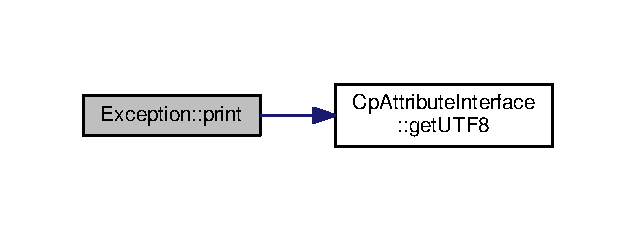
\includegraphics[width=305pt]{class_exception_a87cfd1bc8493cb4b22d9d92a07132779_cgraph}
\end{center}
\end{figure}


\index{Exception@{Exception}!read@{read}}
\index{read@{read}!Exception@{Exception}}
\subsubsection[{\texorpdfstring{read(\+F\+I\+L\+E $\ast$)}{read(FILE *)}}]{\setlength{\rightskip}{0pt plus 5cm}void {\bf Exception\+::read} (
\begin{DoxyParamCaption}
\item[{F\+I\+LE $\ast$}]{fp}
\end{DoxyParamCaption}
)}\hypertarget{class_exception_ad660b6215e7a9df9b2d4bc5216c828c4}{}\label{class_exception_ad660b6215e7a9df9b2d4bc5216c828c4}


Grafo de chamadas desta função\+:
\nopagebreak
\begin{figure}[H]
\begin{center}
\leavevmode
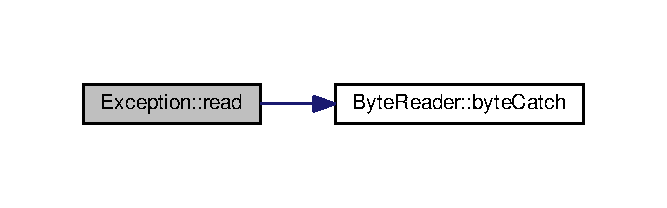
\includegraphics[width=320pt]{class_exception_ad660b6215e7a9df9b2d4bc5216c828c4_cgraph}
\end{center}
\end{figure}




\subsection{Documentação dos dados membro}
\index{Exception@{Exception}!exception\+\_\+index\+\_\+table@{exception\+\_\+index\+\_\+table}}
\index{exception\+\_\+index\+\_\+table@{exception\+\_\+index\+\_\+table}!Exception@{Exception}}
\subsubsection[{\texorpdfstring{exception\+\_\+index\+\_\+table}{exception_index_table}}]{\setlength{\rightskip}{0pt plus 5cm}uint16\+\_\+t$\ast$ Exception\+::exception\+\_\+index\+\_\+table}\hypertarget{class_exception_a496a578392dba7830e8efcc36a27fe27}{}\label{class_exception_a496a578392dba7830e8efcc36a27fe27}
\index{Exception@{Exception}!number\+\_\+exceptions@{number\+\_\+exceptions}}
\index{number\+\_\+exceptions@{number\+\_\+exceptions}!Exception@{Exception}}
\subsubsection[{\texorpdfstring{number\+\_\+exceptions}{number_exceptions}}]{\setlength{\rightskip}{0pt plus 5cm}uint16\+\_\+t Exception\+::number\+\_\+exceptions}\hypertarget{class_exception_add71629097c0b5242c01d1d0d5404d3d}{}\label{class_exception_add71629097c0b5242c01d1d0d5404d3d}


A documentação para esta classe foi gerada a partir dos seguintes ficheiros\+:\begin{DoxyCompactItemize}
\item 
\hyperlink{_attribute_info_8hpp}{Attribute\+Info.\+hpp}\item 
\hyperlink{_attribute_info_8cpp}{Attribute\+Info.\+cpp}\end{DoxyCompactItemize}

\hypertarget{class_interpreter_1_1execute}{}\section{Interpreter\+:\+:execute Class Reference}
\label{class_interpreter_1_1execute}\index{Interpreter\+::execute@{Interpreter\+::execute}}


Carrega o class\+Loader na memória e na stack e executa-\/o.  




\subsection{Detailed Description}
Carrega o class\+Loader na memória e na stack e executa-\/o. 


\begin{DoxyParams}{Parameters}
{\em $\ast$classloader} & ponteiro para \hyperlink{class_class_loader}{Class\+Loader} \\
\hline
\end{DoxyParams}
\begin{DoxyReturn}{Returns}
void 
\end{DoxyReturn}


The documentation for this class was generated from the following file\+:\begin{DoxyCompactItemize}
\item 
\hyperlink{_interpreter_8cpp}{Interpreter.\+cpp}\end{DoxyCompactItemize}

\hypertarget{class_instruction_impl_1_1f2d}{}\section{Instruction\+Impl\+:\+:f2d Class Reference}
\label{class_instruction_impl_1_1f2d}\index{Instruction\+Impl\+::f2d@{Instruction\+Impl\+::f2d}}


Desempilha 1 float da pilha de operandos e o converte para double e empilha o resultado na pilha de operandos.  




\subsection{Detailed Description}
Desempilha 1 float da pilha de operandos e o converte para double e empilha o resultado na pilha de operandos. 


\begin{DoxyParams}{Parameters}
{\em $\ast$this\+\_\+frame} & Ponteiro para o frame atual \\
\hline
\end{DoxyParams}
\begin{DoxyReturn}{Returns}
void 
\end{DoxyReturn}


The documentation for this class was generated from the following file\+:\begin{DoxyCompactItemize}
\item 
\hyperlink{_instruction_impl_8cpp}{Instruction\+Impl.\+cpp}\end{DoxyCompactItemize}

\hypertarget{class_instruction_impl_1_1f2i}{}\section{Instruction\+Impl\+:\+:f2i Class Reference}
\label{class_instruction_impl_1_1f2i}\index{Instruction\+Impl\+::f2i@{Instruction\+Impl\+::f2i}}


Desempilha 1 float da pilha de operandos e o converte para inteiro e empilha o resultado na pilha de operandos.  




\subsection{Detailed Description}
Desempilha 1 float da pilha de operandos e o converte para inteiro e empilha o resultado na pilha de operandos. 


\begin{DoxyParams}{Parameters}
{\em $\ast$this\+\_\+frame} & Ponteiro para o frame atual \\
\hline
\end{DoxyParams}
\begin{DoxyReturn}{Returns}
void 
\end{DoxyReturn}


The documentation for this class was generated from the following file\+:\begin{DoxyCompactItemize}
\item 
\hyperlink{_instruction_impl_8cpp}{Instruction\+Impl.\+cpp}\end{DoxyCompactItemize}

\hypertarget{class_instruction_impl_1_1f2l}{}\section{Instruction\+Impl\+:\+:f2l Class Reference}
\label{class_instruction_impl_1_1f2l}\index{Instruction\+Impl\+::f2l@{Instruction\+Impl\+::f2l}}


converte float para long  




\subsection{Detailed Description}
converte float para long 


\begin{DoxyParams}{Parameters}
{\em this\+\_\+frame} & Ponteiro para frame corrente. \\
\hline
\end{DoxyParams}
\begin{DoxyReturn}{Returns}
void 
\end{DoxyReturn}


The documentation for this class was generated from the following file\+:\begin{DoxyCompactItemize}
\item 
\hyperlink{_instruction_impl_8cpp}{Instruction\+Impl.\+cpp}\end{DoxyCompactItemize}

\hypertarget{class_instruction_impl_1_1fadd}{}\section{Instruction\+Impl\+:\+:fadd Class Reference}
\label{class_instruction_impl_1_1fadd}\index{Instruction\+Impl\+::fadd@{Instruction\+Impl\+::fadd}}


Desempilha dois float da pilha e empilha adição deles.  




\subsection{Detailed Description}
Desempilha dois float da pilha e empilha adição deles. 


\begin{DoxyParams}{Parameters}
{\em $\ast$this\+\_\+frame} & ponteiro para o frame atual \\
\hline
\end{DoxyParams}
\begin{DoxyReturn}{Returns}
void 
\end{DoxyReturn}


The documentation for this class was generated from the following file\+:\begin{DoxyCompactItemize}
\item 
\hyperlink{_instruction_impl_8cpp}{Instruction\+Impl.\+cpp}\end{DoxyCompactItemize}

\hypertarget{class_instruction_impl_1_1faload}{}\section{Referência à classe Instruction\+Impl\+:\+:faload}
\label{class_instruction_impl_1_1faload}\index{Instruction\+Impl\+::faload@{Instruction\+Impl\+::faload}}


Empilha na pilha de operandos um elemento de um array de float.  




\subsection{Descrição detalhada}
Empilha na pilha de operandos um elemento de um array de float. 


\begin{DoxyParams}{Parâmetros}
{\em $\ast$this\+\_\+frame} & Ponteiro para o frame atual \\
\hline
\end{DoxyParams}
\begin{DoxyReturn}{Retorna}
void 
\end{DoxyReturn}


A documentação para esta classe foi gerada a partir do seguinte ficheiro\+:\begin{DoxyCompactItemize}
\item 
\hyperlink{_instruction_impl_8cpp}{Instruction\+Impl.\+cpp}\end{DoxyCompactItemize}

\hypertarget{class_instruction_impl_1_1fastore}{}\section{Instruction\+Impl\+:\+:fastore Class Reference}
\label{class_instruction_impl_1_1fastore}\index{Instruction\+Impl\+::fastore@{Instruction\+Impl\+::fastore}}


Desempilha a referencia para o array, o indice e o valor(float) e salva o valor no array.  




\subsection{Detailed Description}
Desempilha a referencia para o array, o indice e o valor(float) e salva o valor no array. 


\begin{DoxyParams}{Parameters}
{\em $\ast$this\+\_\+frame} & Ponteiro para frame corrente. \\
\hline
\end{DoxyParams}
\begin{DoxyReturn}{Returns}
void 
\end{DoxyReturn}


The documentation for this class was generated from the following file\+:\begin{DoxyCompactItemize}
\item 
\hyperlink{_instruction_impl_8cpp}{Instruction\+Impl.\+cpp}\end{DoxyCompactItemize}

\hypertarget{class_instruction_impl_1_1fcmpg}{}\section{Referência à classe Instruction\+Impl\+:\+:fcmpg}
\label{class_instruction_impl_1_1fcmpg}\index{Instruction\+Impl\+::fcmpg@{Instruction\+Impl\+::fcmpg}}


Função desempilha dois floats, compara ambos e empilha o resultado da comparação. Se são iguais empilha 0, se o segundo número for maior empilha 1, caso contrário empilha -\/1. Caso algum dos números seja NaN, empilha 1.  




\subsection{Descrição detalhada}
Função desempilha dois floats, compara ambos e empilha o resultado da comparação. Se são iguais empilha 0, se o segundo número for maior empilha 1, caso contrário empilha -\/1. Caso algum dos números seja NaN, empilha 1. 


\begin{DoxyParams}{Parâmetros}
{\em $\ast$this\+\_\+frame} & Ponteiro para frame \\
\hline
\end{DoxyParams}
\begin{DoxyReturn}{Retorna}

\end{DoxyReturn}


A documentação para esta classe foi gerada a partir do seguinte ficheiro\+:\begin{DoxyCompactItemize}
\item 
\hyperlink{_instruction_impl_8cpp}{Instruction\+Impl.\+cpp}\end{DoxyCompactItemize}

\hypertarget{class_instruction_impl_1_1fcmpl}{}\section{Referência à classe Instruction\+Impl\+:\+:fcmpl}
\label{class_instruction_impl_1_1fcmpl}\index{Instruction\+Impl\+::fcmpl@{Instruction\+Impl\+::fcmpl}}


Função que desempilha dois floats, compara ambos e empilha o resultado da comparação. 0 se forem iguais, se o segundo número for maior empilha 1, caso contrário empilha -\/1. Caso algum dos números seja NaN, empilha 1.  




\subsection{Descrição detalhada}
Função que desempilha dois floats, compara ambos e empilha o resultado da comparação. 0 se forem iguais, se o segundo número for maior empilha 1, caso contrário empilha -\/1. Caso algum dos números seja NaN, empilha 1. 


\begin{DoxyParams}{Parâmetros}
{\em $\ast$this\+\_\+frame} & \hyperlink{struct_frame}{Frame} corrente. \\
\hline
\end{DoxyParams}
\begin{DoxyReturn}{Retorna}

\end{DoxyReturn}


A documentação para esta classe foi gerada a partir do seguinte ficheiro\+:\begin{DoxyCompactItemize}
\item 
\hyperlink{_instruction_impl_8cpp}{Instruction\+Impl.\+cpp}\end{DoxyCompactItemize}

\hypertarget{class_instruction_impl_1_1fconst__0}{}\section{Referência à classe Instruction\+Impl\+:\+:fconst\+\_\+0}
\label{class_instruction_impl_1_1fconst__0}\index{Instruction\+Impl\+::fconst\+\_\+0@{Instruction\+Impl\+::fconst\+\_\+0}}


Empilha a constante float 0.\+0 na pilha de operandos.  




\subsection{Descrição detalhada}
Empilha a constante float 0.\+0 na pilha de operandos. 


\begin{DoxyParams}{Parâmetros}
{\em $\ast$this\+\_\+frame} & Ponteiro para o frame atual \\
\hline
\end{DoxyParams}
\begin{DoxyReturn}{Retorna}
void 
\end{DoxyReturn}


A documentação para esta classe foi gerada a partir do seguinte ficheiro\+:\begin{DoxyCompactItemize}
\item 
\hyperlink{_instruction_impl_8cpp}{Instruction\+Impl.\+cpp}\end{DoxyCompactItemize}

\hypertarget{class_instruction_impl_1_1fconst__1}{}\section{Instruction\+Impl\+:\+:fconst\+\_\+1 Class Reference}
\label{class_instruction_impl_1_1fconst__1}\index{Instruction\+Impl\+::fconst\+\_\+1@{Instruction\+Impl\+::fconst\+\_\+1}}


Empilha a constante float 1.\+0 na pilha de operandos.  




\subsection{Detailed Description}
Empilha a constante float 1.\+0 na pilha de operandos. 


\begin{DoxyParams}{Parameters}
{\em $\ast$this\+\_\+frame} & Ponteiro para o frame atual \\
\hline
\end{DoxyParams}
\begin{DoxyReturn}{Returns}
void 
\end{DoxyReturn}


The documentation for this class was generated from the following file\+:\begin{DoxyCompactItemize}
\item 
\hyperlink{_instruction_impl_8cpp}{Instruction\+Impl.\+cpp}\end{DoxyCompactItemize}

\hypertarget{class_instruction_impl_1_1fconst__2}{}\section{Referência à classe Instruction\+Impl\+:\+:fconst\+\_\+2}
\label{class_instruction_impl_1_1fconst__2}\index{Instruction\+Impl\+::fconst\+\_\+2@{Instruction\+Impl\+::fconst\+\_\+2}}


Empilha a constante float 2.\+0 na pilha de operandos.  




\subsection{Descrição detalhada}
Empilha a constante float 2.\+0 na pilha de operandos. 


\begin{DoxyParams}{Parâmetros}
{\em $\ast$this\+\_\+frame} & Ponteiro para o frame atual \\
\hline
\end{DoxyParams}
\begin{DoxyReturn}{Retorna}
void 
\end{DoxyReturn}


A documentação para esta classe foi gerada a partir do seguinte ficheiro\+:\begin{DoxyCompactItemize}
\item 
\hyperlink{_instruction_impl_8cpp}{Instruction\+Impl.\+cpp}\end{DoxyCompactItemize}

\hypertarget{class_instruction_impl_1_1fdiv}{}\section{Instruction\+Impl\+:\+:fdiv Class Reference}
\label{class_instruction_impl_1_1fdiv}\index{Instruction\+Impl\+::fdiv@{Instruction\+Impl\+::fdiv}}


Desempilha dois floats da pilha e empilha a divisão deles.  




\subsection{Detailed Description}
Desempilha dois floats da pilha e empilha a divisão deles. 


\begin{DoxyParams}{Parameters}
{\em $\ast$this\+\_\+frame} & ponteiro para o frame atual \\
\hline
\end{DoxyParams}
\begin{DoxyReturn}{Returns}
void 
\end{DoxyReturn}


The documentation for this class was generated from the following file\+:\begin{DoxyCompactItemize}
\item 
\hyperlink{_instruction_impl_8cpp}{Instruction\+Impl.\+cpp}\end{DoxyCompactItemize}

\hypertarget{class_field_info}{}\section{Referência à classe Field\+Info}
\label{class_field_info}\index{Field\+Info@{Field\+Info}}


classe para tratar as fields do .class contém access\+\_\+flags, name\+\_\+index, descriptor\+\_\+index, attributes\+\_\+count e uma array dos atributos a ele designados -\/ tirando a array, todos do tipo uint16 Além disso contém destructor e leitor;  




{\ttfamily \#include $<$Field\+Info.\+hpp$>$}

\subsection*{Componentes}
\begin{DoxyCompactItemize}
\item 
class \hyperlink{class_field_info_1_1read}{read}
\begin{DoxyCompactList}\small\item\em setting inicial do \hyperlink{class_field_info}{Field\+Info} a partir de um arquivo. \end{DoxyCompactList}\item 
class \hyperlink{class_field_info_1_1~_field_info}{$\sim$\+Field\+Info}
\begin{DoxyCompactList}\small\item\em Destrutor de \hyperlink{class_field_info}{Field\+Info}. \end{DoxyCompactList}\end{DoxyCompactItemize}
\subsection*{Membros públicos}
\begin{DoxyCompactItemize}
\item 
\hyperlink{class_field_info_ae59d956e2a4ad2dc210d75f161d5eb31}{$\sim$\+Field\+Info} ()
\item 
void \hyperlink{class_field_info_acb85db9ce893bc3e2617138fd46a8ad6}{read} (F\+I\+LE $\ast$, std\+::vector$<$ \hyperlink{class_cp_info}{Cp\+Info} $\ast$ $>$)
\end{DoxyCompactItemize}
\subsection*{Atributos Públicos}
\begin{DoxyCompactItemize}
\item 
uint16\+\_\+t \hyperlink{class_field_info_a81205117e814694f690cee6271516dc0}{access\+\_\+flags}
\item 
uint16\+\_\+t \hyperlink{class_field_info_a97fd269599826fe99f61ae83311a909c}{name\+\_\+index}
\item 
uint16\+\_\+t \hyperlink{class_field_info_aff3935ae95047693cbe029db915944b9}{descriptor\+\_\+index}
\item 
uint16\+\_\+t \hyperlink{class_field_info_ae559a93403a28923c24eaaeabfcc63c8}{attributes\+\_\+count}
\item 
std\+::vector$<$ \hyperlink{class_attribute_info}{Attribute\+Info} $\ast$ $>$ \hyperlink{class_field_info_ab817d700b4c5cc6f39812c9374022372}{attributes}
\end{DoxyCompactItemize}


\subsection{Descrição detalhada}
classe para tratar as fields do .class contém access\+\_\+flags, name\+\_\+index, descriptor\+\_\+index, attributes\+\_\+count e uma array dos atributos a ele designados -\/ tirando a array, todos do tipo uint16 Além disso contém destructor e leitor; 

\subsection{Documentação dos Construtores \& Destrutor}
\index{Field\+Info@{Field\+Info}!````~Field\+Info@{$\sim$\+Field\+Info}}
\index{````~Field\+Info@{$\sim$\+Field\+Info}!Field\+Info@{Field\+Info}}
\subsubsection[{\texorpdfstring{$\sim$\+Field\+Info()}{~FieldInfo()}}]{\setlength{\rightskip}{0pt plus 5cm}{\bf Field\+Info\+::$\sim$\+Field\+Info} (
\begin{DoxyParamCaption}
{}
\end{DoxyParamCaption}
)}\hypertarget{class_field_info_ae59d956e2a4ad2dc210d75f161d5eb31}{}\label{class_field_info_ae59d956e2a4ad2dc210d75f161d5eb31}


\subsection{Documentação dos métodos}
\index{Field\+Info@{Field\+Info}!read@{read}}
\index{read@{read}!Field\+Info@{Field\+Info}}
\subsubsection[{\texorpdfstring{read(\+F\+I\+L\+E $\ast$, std\+::vector$<$ Cp\+Info $\ast$ $>$)}{read(FILE *, std::vector< CpInfo * >)}}]{\setlength{\rightskip}{0pt plus 5cm}void {\bf Field\+Info\+::read} (
\begin{DoxyParamCaption}
\item[{F\+I\+LE $\ast$}]{fp, }
\item[{std\+::vector$<$ {\bf Cp\+Info} $\ast$ $>$}]{true\+Cp\+Info}
\end{DoxyParamCaption}
)}\hypertarget{class_field_info_acb85db9ce893bc3e2617138fd46a8ad6}{}\label{class_field_info_acb85db9ce893bc3e2617138fd46a8ad6}


Grafo de chamadas desta função\+:
\nopagebreak
\begin{figure}[H]
\begin{center}
\leavevmode
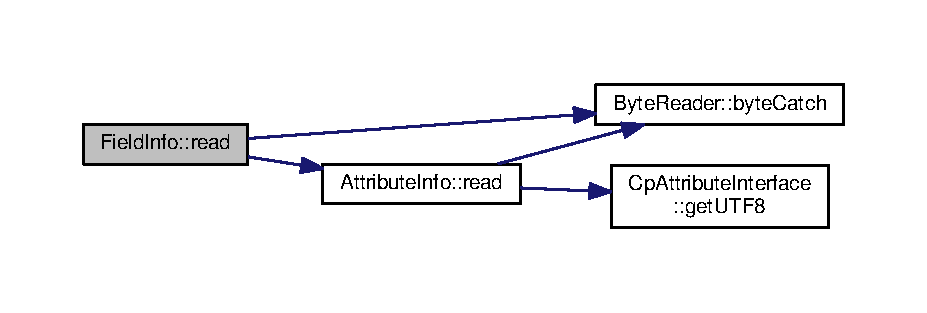
\includegraphics[width=350pt]{class_field_info_acb85db9ce893bc3e2617138fd46a8ad6_cgraph}
\end{center}
\end{figure}




Este é o diagrama das funções que utilizam esta função\+:
\nopagebreak
\begin{figure}[H]
\begin{center}
\leavevmode
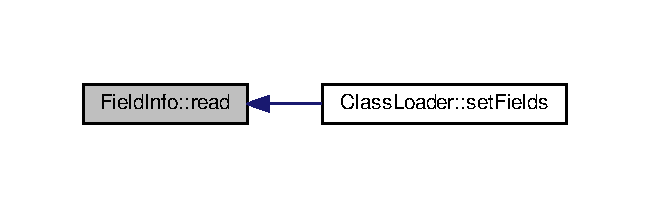
\includegraphics[width=312pt]{class_field_info_acb85db9ce893bc3e2617138fd46a8ad6_icgraph}
\end{center}
\end{figure}




\subsection{Documentação dos dados membro}
\index{Field\+Info@{Field\+Info}!access\+\_\+flags@{access\+\_\+flags}}
\index{access\+\_\+flags@{access\+\_\+flags}!Field\+Info@{Field\+Info}}
\subsubsection[{\texorpdfstring{access\+\_\+flags}{access_flags}}]{\setlength{\rightskip}{0pt plus 5cm}uint16\+\_\+t Field\+Info\+::access\+\_\+flags}\hypertarget{class_field_info_a81205117e814694f690cee6271516dc0}{}\label{class_field_info_a81205117e814694f690cee6271516dc0}
\index{Field\+Info@{Field\+Info}!attributes@{attributes}}
\index{attributes@{attributes}!Field\+Info@{Field\+Info}}
\subsubsection[{\texorpdfstring{attributes}{attributes}}]{\setlength{\rightskip}{0pt plus 5cm}std\+::vector$<${\bf Attribute\+Info} $\ast$$>$ Field\+Info\+::attributes}\hypertarget{class_field_info_ab817d700b4c5cc6f39812c9374022372}{}\label{class_field_info_ab817d700b4c5cc6f39812c9374022372}
\index{Field\+Info@{Field\+Info}!attributes\+\_\+count@{attributes\+\_\+count}}
\index{attributes\+\_\+count@{attributes\+\_\+count}!Field\+Info@{Field\+Info}}
\subsubsection[{\texorpdfstring{attributes\+\_\+count}{attributes_count}}]{\setlength{\rightskip}{0pt plus 5cm}uint16\+\_\+t Field\+Info\+::attributes\+\_\+count}\hypertarget{class_field_info_ae559a93403a28923c24eaaeabfcc63c8}{}\label{class_field_info_ae559a93403a28923c24eaaeabfcc63c8}
\index{Field\+Info@{Field\+Info}!descriptor\+\_\+index@{descriptor\+\_\+index}}
\index{descriptor\+\_\+index@{descriptor\+\_\+index}!Field\+Info@{Field\+Info}}
\subsubsection[{\texorpdfstring{descriptor\+\_\+index}{descriptor_index}}]{\setlength{\rightskip}{0pt plus 5cm}uint16\+\_\+t Field\+Info\+::descriptor\+\_\+index}\hypertarget{class_field_info_aff3935ae95047693cbe029db915944b9}{}\label{class_field_info_aff3935ae95047693cbe029db915944b9}
\index{Field\+Info@{Field\+Info}!name\+\_\+index@{name\+\_\+index}}
\index{name\+\_\+index@{name\+\_\+index}!Field\+Info@{Field\+Info}}
\subsubsection[{\texorpdfstring{name\+\_\+index}{name_index}}]{\setlength{\rightskip}{0pt plus 5cm}uint16\+\_\+t Field\+Info\+::name\+\_\+index}\hypertarget{class_field_info_a97fd269599826fe99f61ae83311a909c}{}\label{class_field_info_a97fd269599826fe99f61ae83311a909c}


A documentação para esta classe foi gerada a partir dos seguintes ficheiros\+:\begin{DoxyCompactItemize}
\item 
\hyperlink{_field_info_8hpp}{Field\+Info.\+hpp}\item 
\hyperlink{_field_info_8cpp}{Field\+Info.\+cpp}\end{DoxyCompactItemize}

\hypertarget{class_instruction_impl_1_1fload}{}\section{Instruction\+Impl\+:\+:fload Class Reference}
\label{class_instruction_impl_1_1fload}\index{Instruction\+Impl\+::fload@{Instruction\+Impl\+::fload}}


Empilha float indicado no indice determinado do array de variáveis locais na pilha de operandos.  




\subsection{Detailed Description}
Empilha float indicado no indice determinado do array de variáveis locais na pilha de operandos. 


\begin{DoxyParams}{Parameters}
{\em $\ast$this\+\_\+frame} & Ponteiro para o frame atual \\
\hline
\end{DoxyParams}
\begin{DoxyReturn}{Returns}
void 
\end{DoxyReturn}


The documentation for this class was generated from the following file\+:\begin{DoxyCompactItemize}
\item 
\hyperlink{_instruction_impl_8cpp}{Instruction\+Impl.\+cpp}\end{DoxyCompactItemize}

\hypertarget{class_instruction_impl_1_1fload__0}{}\section{Instruction\+Impl\+:\+:fload\+\_\+0 Class Reference}
\label{class_instruction_impl_1_1fload__0}\index{Instruction\+Impl\+::fload\+\_\+0@{Instruction\+Impl\+::fload\+\_\+0}}


Empilha float indicado no indice 0 do array de variáveis locais na pilha de operandos.  




\subsection{Detailed Description}
Empilha float indicado no indice 0 do array de variáveis locais na pilha de operandos. 


\begin{DoxyParams}{Parameters}
{\em $\ast$this\+\_\+frame} & Ponteiro para o frame atual \\
\hline
\end{DoxyParams}
\begin{DoxyReturn}{Returns}
void 
\end{DoxyReturn}


The documentation for this class was generated from the following file\+:\begin{DoxyCompactItemize}
\item 
\hyperlink{_instruction_impl_8cpp}{Instruction\+Impl.\+cpp}\end{DoxyCompactItemize}

\hypertarget{class_instruction_impl_1_1fload__1}{}\section{Instruction\+Impl\+:\+:fload\+\_\+1 Class Reference}
\label{class_instruction_impl_1_1fload__1}\index{Instruction\+Impl\+::fload\+\_\+1@{Instruction\+Impl\+::fload\+\_\+1}}


Empilha float indicado no indice 1 do array de variáveis locais na pilha de operandos.  




\subsection{Detailed Description}
Empilha float indicado no indice 1 do array de variáveis locais na pilha de operandos. 


\begin{DoxyParams}{Parameters}
{\em $\ast$this\+\_\+frame} & Ponteiro para o frame atual \\
\hline
\end{DoxyParams}
\begin{DoxyReturn}{Returns}
void 
\end{DoxyReturn}


The documentation for this class was generated from the following file\+:\begin{DoxyCompactItemize}
\item 
\hyperlink{_instruction_impl_8cpp}{Instruction\+Impl.\+cpp}\end{DoxyCompactItemize}

\hypertarget{class_instruction_impl_1_1fload__2}{}\section{Instruction\+Impl\+:\+:fload\+\_\+2 Class Reference}
\label{class_instruction_impl_1_1fload__2}\index{Instruction\+Impl\+::fload\+\_\+2@{Instruction\+Impl\+::fload\+\_\+2}}


Empilha float indicado no indice 2 do array de variáveis locais na pilha de operandos.  




\subsection{Detailed Description}
Empilha float indicado no indice 2 do array de variáveis locais na pilha de operandos. 


\begin{DoxyParams}{Parameters}
{\em $\ast$this\+\_\+frame} & Ponteiro para o frame atual \\
\hline
\end{DoxyParams}
\begin{DoxyReturn}{Returns}
void 
\end{DoxyReturn}


The documentation for this class was generated from the following file\+:\begin{DoxyCompactItemize}
\item 
\hyperlink{_instruction_impl_8cpp}{Instruction\+Impl.\+cpp}\end{DoxyCompactItemize}

\hypertarget{class_instruction_impl_1_1fload__3}{}\section{Referência à classe Instruction\+Impl\+:\+:fload\+\_\+3}
\label{class_instruction_impl_1_1fload__3}\index{Instruction\+Impl\+::fload\+\_\+3@{Instruction\+Impl\+::fload\+\_\+3}}


Empilha float indicado no indice 3 do array de variáveis locais na pilha de operandos.  




\subsection{Descrição detalhada}
Empilha float indicado no indice 3 do array de variáveis locais na pilha de operandos. 


\begin{DoxyParams}{Parâmetros}
{\em $\ast$this\+\_\+frame} & Ponteiro para o frame atual \\
\hline
\end{DoxyParams}
\begin{DoxyReturn}{Retorna}
void 
\end{DoxyReturn}


A documentação para esta classe foi gerada a partir do seguinte ficheiro\+:\begin{DoxyCompactItemize}
\item 
\hyperlink{_instruction_impl_8cpp}{Instruction\+Impl.\+cpp}\end{DoxyCompactItemize}

\hypertarget{class_instruction_impl_1_1fmul}{}\section{Referência à classe Instruction\+Impl\+:\+:fmul}
\label{class_instruction_impl_1_1fmul}\index{Instruction\+Impl\+::fmul@{Instruction\+Impl\+::fmul}}


Desempilha dois floats da pilha e empilha o produto deles.  




\subsection{Descrição detalhada}
Desempilha dois floats da pilha e empilha o produto deles. 


\begin{DoxyParams}{Parâmetros}
{\em $\ast$this\+\_\+frame} & ponteiro para o frame atual \\
\hline
\end{DoxyParams}
\begin{DoxyReturn}{Retorna}
void 
\end{DoxyReturn}


A documentação para esta classe foi gerada a partir do seguinte ficheiro\+:\begin{DoxyCompactItemize}
\item 
\hyperlink{_instruction_impl_8cpp}{Instruction\+Impl.\+cpp}\end{DoxyCompactItemize}

\hypertarget{class_instruction_impl_1_1fneg}{}\section{Instruction\+Impl\+:\+:fneg Class Reference}
\label{class_instruction_impl_1_1fneg}\index{Instruction\+Impl\+::fneg@{Instruction\+Impl\+::fneg}}


Desempilha 1 doubles da pilha de operandos e empilha o valor negativo dele.  




\subsection{Detailed Description}
Desempilha 1 doubles da pilha de operandos e empilha o valor negativo dele. 


\begin{DoxyParams}{Parameters}
{\em $\ast$this\+\_\+frame} & ponteiro para o frame atual \\
\hline
\end{DoxyParams}
\begin{DoxyReturn}{Returns}
void 
\end{DoxyReturn}


The documentation for this class was generated from the following file\+:\begin{DoxyCompactItemize}
\item 
\hyperlink{_instruction_impl_8cpp}{Instruction\+Impl.\+cpp}\end{DoxyCompactItemize}

\hypertarget{struct_frame}{}\section{Frame Struct Reference}
\label{struct_frame}\index{Frame@{Frame}}


objetivo de estruturar o tipo \hyperlink{struct_frame}{Frame}; Além disso, contém destrutor e run(para rodar o frame);  




{\ttfamily \#include $<$Frame.\+hpp$>$}



Collaboration diagram for Frame\+:
% FIG 0
\subsection*{Classes}
\begin{DoxyCompactItemize}
\item 
class \hyperlink{class_frame_1_1_frame}{Frame}
\begin{DoxyCompactList}\small\item\em Construtor de frame, faz a settagem das variáveis do frame. \end{DoxyCompactList}\item 
class \hyperlink{class_frame_1_1run}{run}
\begin{DoxyCompactList}\small\item\em método de execução do código armazenado em um frame. \end{DoxyCompactList}\item 
class \hyperlink{class_frame_1_1~_frame}{$\sim$\+Frame}
\begin{DoxyCompactList}\small\item\em Destrutor de frame, libera o que é alocado no construtor de frame. \end{DoxyCompactList}\end{DoxyCompactItemize}
\subsection*{Public Member Functions}
\begin{DoxyCompactItemize}
\item 
\hyperlink{struct_frame_abe0b370087d05267cab997ecdc78c4bd}{Frame} (std\+::vector$<$ \hyperlink{class_cp_info}{Cp\+Info} $\ast$ $>$, \hyperlink{struct_method_info}{Method\+Info} $\ast$)
\item 
\hyperlink{struct_frame_abec8c7bccdfc88cb4da137caae9f73d6}{$\sim$\+Frame} ()
\item 
void \hyperlink{struct_frame_a9aa2ef354e013a7cb95827c55a3b3a95}{run} ()
\end{DoxyCompactItemize}
\subsection*{Public Attributes}
\begin{DoxyCompactItemize}
\item 
uint32\+\_\+t \hyperlink{struct_frame_a91e50d2091184efb52b6d7c0c21fd4b2}{pc}
\item 
std\+::stack$<$ \hyperlink{struct_operand}{Operand} $\ast$ $>$ \hyperlink{struct_frame_a30eaf6634fbadf9dd4c6a8c05b92d3a4}{operand\+\_\+stack}
\item 
\hyperlink{class_code_attribute}{Code\+Attribute} \hyperlink{struct_frame_a7eac6c489fcfc2de43409f405d360a3d}{method\+\_\+code}
\item 
\hyperlink{struct_method_info}{Method\+Info} $\ast$ \hyperlink{struct_frame_ad7c3164833be265d690a786a172ca80a}{method\+\_\+reference}
\item 
std\+::vector$<$ \hyperlink{class_cp_info}{Cp\+Info} $\ast$ $>$ \hyperlink{struct_frame_af1f36df4b5e662589ccf18d253318060}{cp\+\_\+reference}
\item 
std\+::vector$<$ \hyperlink{struct_operand}{Operand} $\ast$ $>$ \hyperlink{struct_frame_aed517b3bbbefabb20d8e990623ac3118}{local\+\_\+variables}
\item 
\hyperlink{class_instruction}{Instruction} $\ast$ \hyperlink{struct_frame_a831ef5a24bea9ba519495aa41e2f2a7e}{instructions}
\end{DoxyCompactItemize}


\subsection{Detailed Description}
objetivo de estruturar o tipo \hyperlink{struct_frame}{Frame}; Além disso, contém destrutor e run(para rodar o frame); 

\subsection{Constructor \& Destructor Documentation}
\index{Frame@{Frame}!Frame@{Frame}}
\index{Frame@{Frame}!Frame@{Frame}}
\subsubsection[{\texorpdfstring{Frame(std\+::vector$<$ Cp\+Info $\ast$ $>$, Method\+Info $\ast$)}{Frame(std::vector< CpInfo * >, MethodInfo *)}}]{\setlength{\rightskip}{0pt plus 5cm}{\bf Frame\+::\+Frame} (
\begin{DoxyParamCaption}
\item[{std\+::vector$<$ {\bf Cp\+Info} $\ast$ $>$}]{cp, }
\item[{{\bf Method\+Info} $\ast$}]{methd}
\end{DoxyParamCaption}
)}\hypertarget{struct_frame_abe0b370087d05267cab997ecdc78c4bd}{}\label{struct_frame_abe0b370087d05267cab997ecdc78c4bd}


Here is the call graph for this function\+:
% FIG 1


\index{Frame@{Frame}!````~Frame@{$\sim$\+Frame}}
\index{````~Frame@{$\sim$\+Frame}!Frame@{Frame}}
\subsubsection[{\texorpdfstring{$\sim$\+Frame()}{~Frame()}}]{\setlength{\rightskip}{0pt plus 5cm}{\bf Frame\+::$\sim$\+Frame} (
\begin{DoxyParamCaption}
{}
\end{DoxyParamCaption}
)}\hypertarget{struct_frame_abec8c7bccdfc88cb4da137caae9f73d6}{}\label{struct_frame_abec8c7bccdfc88cb4da137caae9f73d6}


\subsection{Member Function Documentation}
\index{Frame@{Frame}!run@{run}}
\index{run@{run}!Frame@{Frame}}
\subsubsection[{\texorpdfstring{run()}{run()}}]{\setlength{\rightskip}{0pt plus 5cm}void {\bf Frame\+::run} (
\begin{DoxyParamCaption}
{}
\end{DoxyParamCaption}
)}\hypertarget{struct_frame_a9aa2ef354e013a7cb95827c55a3b3a95}{}\label{struct_frame_a9aa2ef354e013a7cb95827c55a3b3a95}


\subsection{Member Data Documentation}
\index{Frame@{Frame}!cp\+\_\+reference@{cp\+\_\+reference}}
\index{cp\+\_\+reference@{cp\+\_\+reference}!Frame@{Frame}}
\subsubsection[{\texorpdfstring{cp\+\_\+reference}{cp_reference}}]{\setlength{\rightskip}{0pt plus 5cm}std\+::vector$<${\bf Cp\+Info}$\ast$$>$ Frame\+::cp\+\_\+reference}\hypertarget{struct_frame_af1f36df4b5e662589ccf18d253318060}{}\label{struct_frame_af1f36df4b5e662589ccf18d253318060}
\index{Frame@{Frame}!instructions@{instructions}}
\index{instructions@{instructions}!Frame@{Frame}}
\subsubsection[{\texorpdfstring{instructions}{instructions}}]{\setlength{\rightskip}{0pt plus 5cm}{\bf Instruction}$\ast$ Frame\+::instructions}\hypertarget{struct_frame_a831ef5a24bea9ba519495aa41e2f2a7e}{}\label{struct_frame_a831ef5a24bea9ba519495aa41e2f2a7e}
\index{Frame@{Frame}!local\+\_\+variables@{local\+\_\+variables}}
\index{local\+\_\+variables@{local\+\_\+variables}!Frame@{Frame}}
\subsubsection[{\texorpdfstring{local\+\_\+variables}{local_variables}}]{\setlength{\rightskip}{0pt plus 5cm}std\+::vector$<$ {\bf Operand}$\ast$ $>$ Frame\+::local\+\_\+variables}\hypertarget{struct_frame_aed517b3bbbefabb20d8e990623ac3118}{}\label{struct_frame_aed517b3bbbefabb20d8e990623ac3118}
\index{Frame@{Frame}!method\+\_\+code@{method\+\_\+code}}
\index{method\+\_\+code@{method\+\_\+code}!Frame@{Frame}}
\subsubsection[{\texorpdfstring{method\+\_\+code}{method_code}}]{\setlength{\rightskip}{0pt plus 5cm}{\bf Code\+Attribute} Frame\+::method\+\_\+code}\hypertarget{struct_frame_a7eac6c489fcfc2de43409f405d360a3d}{}\label{struct_frame_a7eac6c489fcfc2de43409f405d360a3d}
\index{Frame@{Frame}!method\+\_\+reference@{method\+\_\+reference}}
\index{method\+\_\+reference@{method\+\_\+reference}!Frame@{Frame}}
\subsubsection[{\texorpdfstring{method\+\_\+reference}{method_reference}}]{\setlength{\rightskip}{0pt plus 5cm}{\bf Method\+Info}$\ast$ Frame\+::method\+\_\+reference}\hypertarget{struct_frame_ad7c3164833be265d690a786a172ca80a}{}\label{struct_frame_ad7c3164833be265d690a786a172ca80a}
\index{Frame@{Frame}!operand\+\_\+stack@{operand\+\_\+stack}}
\index{operand\+\_\+stack@{operand\+\_\+stack}!Frame@{Frame}}
\subsubsection[{\texorpdfstring{operand\+\_\+stack}{operand_stack}}]{\setlength{\rightskip}{0pt plus 5cm}std\+::stack$<$ {\bf Operand}$\ast$$>$ Frame\+::operand\+\_\+stack}\hypertarget{struct_frame_a30eaf6634fbadf9dd4c6a8c05b92d3a4}{}\label{struct_frame_a30eaf6634fbadf9dd4c6a8c05b92d3a4}
\index{Frame@{Frame}!pc@{pc}}
\index{pc@{pc}!Frame@{Frame}}
\subsubsection[{\texorpdfstring{pc}{pc}}]{\setlength{\rightskip}{0pt plus 5cm}uint32\+\_\+t Frame\+::pc}\hypertarget{struct_frame_a91e50d2091184efb52b6d7c0c21fd4b2}{}\label{struct_frame_a91e50d2091184efb52b6d7c0c21fd4b2}


The documentation for this struct was generated from the following files\+:\begin{DoxyCompactItemize}
\item 
\hyperlink{_frame_8hpp}{Frame.\+hpp}\item 
\hyperlink{_frame_8cpp}{Frame.\+cpp}\end{DoxyCompactItemize}

\hypertarget{class_frame_1_1_frame}{}\section{Referência à classe Frame\+:\+:Frame}
\label{class_frame_1_1_frame}\index{Frame\+::\+Frame@{Frame\+::\+Frame}}


Construtor de frame, faz a settagem das variáveis do frame.  




\subsection{Descrição detalhada}
Construtor de frame, faz a settagem das variáveis do frame. 


\begin{DoxyParams}{Parâmetros}
{\em cp} & vetor de de Cp\+Info$\ast$ \\
\hline
{\em methd} & método sobre o qual o frame será criado. \\
\hline
\end{DoxyParams}
\begin{DoxyReturn}{Retorna}

\end{DoxyReturn}


A documentação para esta classe foi gerada a partir do seguinte ficheiro\+:\begin{DoxyCompactItemize}
\item 
\hyperlink{_frame_8cpp}{Frame.\+cpp}\end{DoxyCompactItemize}

\hypertarget{class_instruction_impl_1_1frem}{}\section{Instruction\+Impl\+:\+:frem Class Reference}
\label{class_instruction_impl_1_1frem}\index{Instruction\+Impl\+::frem@{Instruction\+Impl\+::frem}}


Desempilha dois floats da pilha e empilha resto da divisão entre eles.  




\subsection{Detailed Description}
Desempilha dois floats da pilha e empilha resto da divisão entre eles. 


\begin{DoxyParams}{Parameters}
{\em $\ast$this\+\_\+frame} & ponteiro para o frame atual \\
\hline
\end{DoxyParams}
\begin{DoxyReturn}{Returns}
void 
\end{DoxyReturn}


The documentation for this class was generated from the following file\+:\begin{DoxyCompactItemize}
\item 
\hyperlink{_instruction_impl_8cpp}{Instruction\+Impl.\+cpp}\end{DoxyCompactItemize}

\hypertarget{class_instruction_impl_1_1freturn}{}\section{Instruction\+Impl\+:\+:freturn Class Reference}
\label{class_instruction_impl_1_1freturn}\index{Instruction\+Impl\+::freturn@{Instruction\+Impl\+::freturn}}


Retorna float de um método.  




\subsection{Detailed Description}
Retorna float de um método. 


\begin{DoxyParams}{Parameters}
{\em $\ast$this\+\_\+frame} & ponteiro para o frame atual \\
\hline
\end{DoxyParams}
\begin{DoxyReturn}{Returns}
void 
\end{DoxyReturn}


The documentation for this class was generated from the following file\+:\begin{DoxyCompactItemize}
\item 
\hyperlink{_instruction_impl_8cpp}{Instruction\+Impl.\+cpp}\end{DoxyCompactItemize}

\hypertarget{class_instruction_impl_1_1fstore}{}\section{Referência à classe Instruction\+Impl\+:\+:fstore}
\label{class_instruction_impl_1_1fstore}\index{Instruction\+Impl\+::fstore@{Instruction\+Impl\+::fstore}}


Armazena float do topo da pilha de operandos no array de variaveis locais.  




\subsection{Descrição detalhada}
Armazena float do topo da pilha de operandos no array de variaveis locais. 


\begin{DoxyParams}{Parâmetros}
{\em $\ast$this\+\_\+frame} & Ponteiro para o frame atual \\
\hline
\end{DoxyParams}
\begin{DoxyReturn}{Retorna}
void 
\end{DoxyReturn}


A documentação para esta classe foi gerada a partir do seguinte ficheiro\+:\begin{DoxyCompactItemize}
\item 
\hyperlink{_instruction_impl_8cpp}{Instruction\+Impl.\+cpp}\end{DoxyCompactItemize}

\hypertarget{class_instruction_impl_1_1fstore__0}{}\section{Instruction\+Impl\+:\+:fstore\+\_\+0 Class Reference}
\label{class_instruction_impl_1_1fstore__0}\index{Instruction\+Impl\+::fstore\+\_\+0@{Instruction\+Impl\+::fstore\+\_\+0}}


Armazena float do topo da pilha de operandos no array de variaveis locais no indice 0.  




\subsection{Detailed Description}
Armazena float do topo da pilha de operandos no array de variaveis locais no indice 0. 


\begin{DoxyParams}{Parameters}
{\em $\ast$this\+\_\+frame} & Ponteiro para o frame atual \\
\hline
\end{DoxyParams}
\begin{DoxyReturn}{Returns}
void 
\end{DoxyReturn}


The documentation for this class was generated from the following file\+:\begin{DoxyCompactItemize}
\item 
\hyperlink{_instruction_impl_8cpp}{Instruction\+Impl.\+cpp}\end{DoxyCompactItemize}

\hypertarget{class_instruction_impl_1_1fstore__1}{}\section{Instruction\+Impl\+:\+:fstore\+\_\+1 Class Reference}
\label{class_instruction_impl_1_1fstore__1}\index{Instruction\+Impl\+::fstore\+\_\+1@{Instruction\+Impl\+::fstore\+\_\+1}}


Armazena float do topo da pilha de operandos no array de variaveis locais no indice 1.  




\subsection{Detailed Description}
Armazena float do topo da pilha de operandos no array de variaveis locais no indice 1. 


\begin{DoxyParams}{Parameters}
{\em $\ast$this\+\_\+frame} & Ponteiro para o frame atual \\
\hline
\end{DoxyParams}
\begin{DoxyReturn}{Returns}
void 
\end{DoxyReturn}


The documentation for this class was generated from the following file\+:\begin{DoxyCompactItemize}
\item 
\hyperlink{_instruction_impl_8cpp}{Instruction\+Impl.\+cpp}\end{DoxyCompactItemize}

\hypertarget{class_instruction_impl_1_1fstore__2}{}\section{Referência à classe Instruction\+Impl\+:\+:fstore\+\_\+2}
\label{class_instruction_impl_1_1fstore__2}\index{Instruction\+Impl\+::fstore\+\_\+2@{Instruction\+Impl\+::fstore\+\_\+2}}


Armazena float do topo da pilha de operandos no array de variaveis locais no indice 2.  




\subsection{Descrição detalhada}
Armazena float do topo da pilha de operandos no array de variaveis locais no indice 2. 


\begin{DoxyParams}{Parâmetros}
{\em $\ast$this\+\_\+frame} & Ponteiro para o frame atual \\
\hline
\end{DoxyParams}
\begin{DoxyReturn}{Retorna}
void 
\end{DoxyReturn}


A documentação para esta classe foi gerada a partir do seguinte ficheiro\+:\begin{DoxyCompactItemize}
\item 
\hyperlink{_instruction_impl_8cpp}{Instruction\+Impl.\+cpp}\end{DoxyCompactItemize}

\hypertarget{class_instruction_impl_1_1fstore__3}{}\section{Referência à classe Instruction\+Impl\+:\+:fstore\+\_\+3}
\label{class_instruction_impl_1_1fstore__3}\index{Instruction\+Impl\+::fstore\+\_\+3@{Instruction\+Impl\+::fstore\+\_\+3}}


Armazena float do topo da pilha de operandos no array de variaveis locais no indice 3.  




\subsection{Descrição detalhada}
Armazena float do topo da pilha de operandos no array de variaveis locais no indice 3. 


\begin{DoxyParams}{Parâmetros}
{\em $\ast$this\+\_\+frame} & Ponteiro para o frame atual \\
\hline
\end{DoxyParams}
\begin{DoxyReturn}{Retorna}
void 
\end{DoxyReturn}


A documentação para esta classe foi gerada a partir do seguinte ficheiro\+:\begin{DoxyCompactItemize}
\item 
\hyperlink{_instruction_impl_8cpp}{Instruction\+Impl.\+cpp}\end{DoxyCompactItemize}

\hypertarget{class_instruction_impl_1_1fsub}{}\section{Referência à classe Instruction\+Impl\+:\+:fsub}
\label{class_instruction_impl_1_1fsub}\index{Instruction\+Impl\+::fsub@{Instruction\+Impl\+::fsub}}


Desempilha dois floats da pilha e empilha subtração deles.  




\subsection{Descrição detalhada}
Desempilha dois floats da pilha e empilha subtração deles. 


\begin{DoxyParams}{Parâmetros}
{\em $\ast$this\+\_\+frame} & ponteiro para o frame atual \\
\hline
\end{DoxyParams}
\begin{DoxyReturn}{Retorna}
void 
\end{DoxyReturn}


A documentação para esta classe foi gerada a partir do seguinte ficheiro\+:\begin{DoxyCompactItemize}
\item 
\hyperlink{_instruction_impl_8cpp}{Instruction\+Impl.\+cpp}\end{DoxyCompactItemize}

\hypertarget{class_class_loader_1_1get_attributes}{}\section{Referência à classe Class\+Loader\+:\+:get\+Attributes}
\label{class_class_loader_1_1get_attributes}\index{Class\+Loader\+::get\+Attributes@{Class\+Loader\+::get\+Attributes}}


Método que retona os attributes\+\_\+info ;.  




\subsection{Descrição detalhada}
Método que retona os attributes\+\_\+info ;. 


\begin{DoxyParams}{Parâmetros}
{\em Arquivo} & .class \\
\hline
\end{DoxyParams}
\begin{DoxyReturn}{Retorna}
Attribute\+\_\+info 
\end{DoxyReturn}


A documentação para esta classe foi gerada a partir do seguinte ficheiro\+:\begin{DoxyCompactItemize}
\item 
\hyperlink{_class_loader_8cpp}{Class\+Loader.\+cpp}\end{DoxyCompactItemize}

\hypertarget{class_interpreter_1_1get_class_info}{}\section{Interpreter\+:\+:get\+Class\+Info Class Reference}
\label{class_interpreter_1_1get_class_info}\index{Interpreter\+::get\+Class\+Info@{Interpreter\+::get\+Class\+Info}}


Acessa a memória em busca de uma classe, caso inexistente, carrega a classe buscada em memória.  




\subsection{Detailed Description}
Acessa a memória em busca de uma classe, caso inexistente, carrega a classe buscada em memória. 


\begin{DoxyParams}{Parameters}
{\em class\+Name} & nome da classe buscada. \\
\hline
\end{DoxyParams}
\begin{DoxyReturn}{Returns}
void 
\end{DoxyReturn}


The documentation for this class was generated from the following file\+:\begin{DoxyCompactItemize}
\item 
\hyperlink{_interpreter_8cpp}{Interpreter.\+cpp}\end{DoxyCompactItemize}

\hypertarget{class_instruction_impl_1_1getfield}{}\section{Referência à classe Instruction\+Impl\+:\+:getfield}
\label{class_instruction_impl_1_1getfield}\index{Instruction\+Impl\+::getfield@{Instruction\+Impl\+::getfield}}


Busca o campo de um objeto.  




\subsection{Descrição detalhada}
Busca o campo de um objeto. 


\begin{DoxyParams}{Parâmetros}
{\em $\ast$this\+\_\+frame} & ponteiro para o frame atual \\
\hline
\end{DoxyParams}
\begin{DoxyReturn}{Retorna}
void 
\end{DoxyReturn}


A documentação para esta classe foi gerada a partir do seguinte ficheiro\+:\begin{DoxyCompactItemize}
\item 
\hyperlink{_instruction_impl_8cpp}{Instruction\+Impl.\+cpp}\end{DoxyCompactItemize}

\hypertarget{class_class_loader_1_1get_fields}{}\section{Class\+Loader\+:\+:get\+Fields Class Reference}
\label{class_class_loader_1_1get_fields}\index{Class\+Loader\+::get\+Fields@{Class\+Loader\+::get\+Fields}}


Método que retona os field\+\_\+info ;.  




\subsection{Detailed Description}
Método que retona os field\+\_\+info ;. 


\begin{DoxyParams}{Parameters}
{\em Arquivo} & .class \\
\hline
\end{DoxyParams}
\begin{DoxyReturn}{Returns}
Field\+\_\+info 
\end{DoxyReturn}


The documentation for this class was generated from the following file\+:\begin{DoxyCompactItemize}
\item 
\hyperlink{_class_loader_8cpp}{Class\+Loader.\+cpp}\end{DoxyCompactItemize}

\hypertarget{class_class_loader_1_1get_methods}{}\section{Class\+Loader\+:\+:get\+Methods Class Reference}
\label{class_class_loader_1_1get_methods}\index{Class\+Loader\+::get\+Methods@{Class\+Loader\+::get\+Methods}}


Método que retona os methods\+\_\+info ;.  




\subsection{Detailed Description}
Método que retona os methods\+\_\+info ;. 


\begin{DoxyParams}{Parameters}
{\em Arquivo} & .class \\
\hline
\end{DoxyParams}
\begin{DoxyReturn}{Returns}
Field\+\_\+info 
\end{DoxyReturn}


The documentation for this class was generated from the following file\+:\begin{DoxyCompactItemize}
\item 
\hyperlink{_class_loader_8cpp}{Class\+Loader.\+cpp}\end{DoxyCompactItemize}

\hypertarget{class_instruction_impl_1_1getstatic}{}\section{Instruction\+Impl\+:\+:getstatic Class Reference}
\label{class_instruction_impl_1_1getstatic}\index{Instruction\+Impl\+::getstatic@{Instruction\+Impl\+::getstatic}}


Carrega as classes estáticas na pilha para a execução.  




\subsection{Detailed Description}
Carrega as classes estáticas na pilha para a execução. 


\begin{DoxyParams}{Parameters}
{\em $\ast$this\+\_\+frame} & ponteiro para o frame atual. \\
\hline
\end{DoxyParams}
\begin{DoxyReturn}{Returns}
void 
\end{DoxyReturn}


The documentation for this class was generated from the following file\+:\begin{DoxyCompactItemize}
\item 
\hyperlink{_instruction_impl_8cpp}{Instruction\+Impl.\+cpp}\end{DoxyCompactItemize}

\hypertarget{class_methods_area_1_1get_staticfield}{}\section{Referência à classe Methods\+Area\+:\+:get\+Staticfield}
\label{class_methods_area_1_1get_staticfield}\index{Methods\+Area\+::get\+Staticfield@{Methods\+Area\+::get\+Staticfield}}


Retorna uma variável de uma classe especifica.  




\subsection{Descrição detalhada}
Retorna uma variável de uma classe especifica. 


\begin{DoxyParams}{Parâmetros}
{\em class\+Name} & nome da classe \\
\hline
{\em var\+Name} & nome da variável. \\
\hline
\end{DoxyParams}
\begin{DoxyReturn}{Retorna}
Operand$\ast$ 
\end{DoxyReturn}


A documentação para esta classe foi gerada a partir do seguinte ficheiro\+:\begin{DoxyCompactItemize}
\item 
\hyperlink{_g_l_o_b_a_l__file_8cpp}{G\+L\+O\+B\+A\+L\+\_\+file.\+cpp}\end{DoxyCompactItemize}

\hypertarget{class_cp_attribute_interface_1_1get_u_t_f8}{}\section{Referência à classe Cp\+Attribute\+Interface\+:\+:get\+U\+T\+F8}
\label{class_cp_attribute_interface_1_1get_u_t_f8}\index{Cp\+Attribute\+Interface\+::get\+U\+T\+F8@{Cp\+Attribute\+Interface\+::get\+U\+T\+F8}}


Função que realiza buscas recursivas dentro do \hyperlink{class_cp_info}{Cp\+Info} de um bytecode.  




\subsection{Descrição detalhada}
Função que realiza buscas recursivas dentro do \hyperlink{class_cp_info}{Cp\+Info} de um bytecode. 


\begin{DoxyParams}{Parâmetros}
{\em alpha} & vetor de Cp\+Info$\ast$ \\
\hline
{\em beta} & index de início da busca. \\
\hline
\end{DoxyParams}
\begin{DoxyReturn}{Retorna}
std\+::string 
\end{DoxyReturn}


A documentação para esta classe foi gerada a partir do seguinte ficheiro\+:\begin{DoxyCompactItemize}
\item 
\hyperlink{_cp_attribute_interface_8cpp}{Cp\+Attribute\+Interface.\+cpp}\end{DoxyCompactItemize}

\hypertarget{class_instruction_impl_1_1goto__w}{}\section{Referência à classe Instruction\+Impl\+:\+:goto\+\_\+w}
\label{class_instruction_impl_1_1goto__w}\index{Instruction\+Impl\+::goto\+\_\+w@{Instruction\+Impl\+::goto\+\_\+w}}


Instruçao que executa o desvio para determinado endereco com mais bytes.  




\subsection{Descrição detalhada}
Instruçao que executa o desvio para determinado endereco com mais bytes. 


\begin{DoxyParams}{Parâmetros}
{\em $\ast$this\+\_\+frame} & ponteiro para o frame atual \\
\hline
\end{DoxyParams}
\begin{DoxyReturn}{Retorna}
void 
\end{DoxyReturn}


A documentação para esta classe foi gerada a partir do seguinte ficheiro\+:\begin{DoxyCompactItemize}
\item 
\hyperlink{_instruction_impl_8cpp}{Instruction\+Impl.\+cpp}\end{DoxyCompactItemize}

\hypertarget{class_instruction_impl_1_1i2b}{}\section{Referência à classe Instruction\+Impl\+:\+:i2b}
\label{class_instruction_impl_1_1i2b}\index{Instruction\+Impl\+::i2b@{Instruction\+Impl\+::i2b}}


Função convert um inteiro para byte.  




\subsection{Descrição detalhada}
Função convert um inteiro para byte. 


\begin{DoxyParams}{Parâmetros}
{\em $\ast$this\+\_\+frame} & Ponteiro para Ponteiro para frame. \\
\hline
\end{DoxyParams}
\begin{DoxyReturn}{Retorna}

\end{DoxyReturn}


A documentação para esta classe foi gerada a partir do seguinte ficheiro\+:\begin{DoxyCompactItemize}
\item 
\hyperlink{_instruction_impl_8cpp}{Instruction\+Impl.\+cpp}\end{DoxyCompactItemize}

\hypertarget{class_instruction_impl_1_1i2c}{}\section{Instruction\+Impl\+:\+:i2c Class Reference}
\label{class_instruction_impl_1_1i2c}\index{Instruction\+Impl\+::i2c@{Instruction\+Impl\+::i2c}}


Função que desempilha um inteiro, converte para char e empilha novamente.  




\subsection{Detailed Description}
Função que desempilha um inteiro, converte para char e empilha novamente. 


\begin{DoxyParams}{Parameters}
{\em frame} & Ponteiro para frame. \\
\hline
\end{DoxyParams}
\begin{DoxyReturn}{Returns}

\end{DoxyReturn}


The documentation for this class was generated from the following file\+:\begin{DoxyCompactItemize}
\item 
\hyperlink{_instruction_impl_8cpp}{Instruction\+Impl.\+cpp}\end{DoxyCompactItemize}

\hypertarget{class_instruction_impl_1_1i2d}{}\section{Instruction\+Impl\+:\+:i2d Class Reference}
\label{class_instruction_impl_1_1i2d}\index{Instruction\+Impl\+::i2d@{Instruction\+Impl\+::i2d}}


Função que desempilha um inteiro, converte para double e empilha novamente.  




\subsection{Detailed Description}
Função que desempilha um inteiro, converte para double e empilha novamente. 


\begin{DoxyParams}{Parameters}
{\em this\+\_\+frame} & Ponteiro para frame. \\
\hline
\end{DoxyParams}
\begin{DoxyReturn}{Returns}

\end{DoxyReturn}


The documentation for this class was generated from the following file\+:\begin{DoxyCompactItemize}
\item 
\hyperlink{_instruction_impl_8cpp}{Instruction\+Impl.\+cpp}\end{DoxyCompactItemize}

\hypertarget{class_instruction_impl_1_1i2f}{}\section{Instruction\+Impl\+:\+:i2f Class Reference}
\label{class_instruction_impl_1_1i2f}\index{Instruction\+Impl\+::i2f@{Instruction\+Impl\+::i2f}}


Converte de inteiro para float.  




\subsection{Detailed Description}
Converte de inteiro para float. 


\begin{DoxyParams}{Parameters}
{\em $\ast$this\+\_\+frame} & ponteiro para o frame atual \\
\hline
\end{DoxyParams}
\begin{DoxyReturn}{Returns}
void 
\end{DoxyReturn}


The documentation for this class was generated from the following file\+:\begin{DoxyCompactItemize}
\item 
\hyperlink{_instruction_impl_8cpp}{Instruction\+Impl.\+cpp}\end{DoxyCompactItemize}

\hypertarget{class_instruction_impl_1_1i2l}{}\section{Instruction\+Impl\+:\+:i2l Class Reference}
\label{class_instruction_impl_1_1i2l}\index{Instruction\+Impl\+::i2l@{Instruction\+Impl\+::i2l}}


Função convert operando inteiro long e empilha novamente.  




\subsection{Detailed Description}
Função convert operando inteiro long e empilha novamente. 


\begin{DoxyParams}{Parameters}
{\em $\ast$this\+\_\+frame} & ponteiro para frame atual. \\
\hline
\end{DoxyParams}
\begin{DoxyReturn}{Returns}

\end{DoxyReturn}


The documentation for this class was generated from the following file\+:\begin{DoxyCompactItemize}
\item 
\hyperlink{_instruction_impl_8cpp}{Instruction\+Impl.\+cpp}\end{DoxyCompactItemize}

\hypertarget{class_instruction_impl_1_1i2s}{}\section{Instruction\+Impl\+:\+:i2s Class Reference}
\label{class_instruction_impl_1_1i2s}\index{Instruction\+Impl\+::i2s@{Instruction\+Impl\+::i2s}}


Função que desempilha um inteiro, converte para short e empilha novamente.  




\subsection{Detailed Description}
Função que desempilha um inteiro, converte para short e empilha novamente. 


\begin{DoxyParams}{Parameters}
{\em frame} & Ponteiro para frame. \\
\hline
\end{DoxyParams}
\begin{DoxyReturn}{Returns}
void 
\end{DoxyReturn}


The documentation for this class was generated from the following file\+:\begin{DoxyCompactItemize}
\item 
\hyperlink{_instruction_impl_8cpp}{Instruction\+Impl.\+cpp}\end{DoxyCompactItemize}

\hypertarget{class_instruction_impl_1_1i__goto}{}\section{Referência à classe Instruction\+Impl\+:\+:i\+\_\+goto}
\label{class_instruction_impl_1_1i__goto}\index{Instruction\+Impl\+::i\+\_\+goto@{Instruction\+Impl\+::i\+\_\+goto}}


Instruçao que executa o desvio para determinado endereco.  




\subsection{Descrição detalhada}
Instruçao que executa o desvio para determinado endereco. 


\begin{DoxyParams}{Parâmetros}
{\em $\ast$this\+\_\+frame} & ponteiro para o frame atual \\
\hline
\end{DoxyParams}
\begin{DoxyReturn}{Retorna}
void 
\end{DoxyReturn}


A documentação para esta classe foi gerada a partir do seguinte ficheiro\+:\begin{DoxyCompactItemize}
\item 
\hyperlink{_instruction_impl_8cpp}{Instruction\+Impl.\+cpp}\end{DoxyCompactItemize}

\hypertarget{class_instruction_impl_1_1iadd}{}\section{Instruction\+Impl\+:\+:iadd Class Reference}
\label{class_instruction_impl_1_1iadd}\index{Instruction\+Impl\+::iadd@{Instruction\+Impl\+::iadd}}


Desempilha 2 inteiros da pilha de operandos e empilha a soma deles.  




\subsection{Detailed Description}
Desempilha 2 inteiros da pilha de operandos e empilha a soma deles. 


\begin{DoxyParams}{Parameters}
{\em $\ast$this\+\_\+frame} & ponteiro para o frame atual \\
\hline
\end{DoxyParams}
\begin{DoxyReturn}{Returns}
void 
\end{DoxyReturn}


The documentation for this class was generated from the following file\+:\begin{DoxyCompactItemize}
\item 
\hyperlink{_instruction_impl_8cpp}{Instruction\+Impl.\+cpp}\end{DoxyCompactItemize}

\hypertarget{class_instruction_impl_1_1iaload}{}\section{Instruction\+Impl\+:\+:iaload Class Reference}
\label{class_instruction_impl_1_1iaload}\index{Instruction\+Impl\+::iaload@{Instruction\+Impl\+::iaload}}


Empilha na pilha de operandos um elemento de um array de inteiros.  




\subsection{Detailed Description}
Empilha na pilha de operandos um elemento de um array de inteiros. 


\begin{DoxyParams}{Parameters}
{\em $\ast$this\+\_\+frame} & Ponteiro para o frame atual \\
\hline
\end{DoxyParams}
\begin{DoxyReturn}{Returns}
void 
\end{DoxyReturn}


The documentation for this class was generated from the following file\+:\begin{DoxyCompactItemize}
\item 
\hyperlink{_instruction_impl_8cpp}{Instruction\+Impl.\+cpp}\end{DoxyCompactItemize}

\hypertarget{class_instruction_impl_1_1iand}{}\section{Instruction\+Impl\+:\+:iand Class Reference}
\label{class_instruction_impl_1_1iand}\index{Instruction\+Impl\+::iand@{Instruction\+Impl\+::iand}}


Desempilha dois valores inteiros da pilha, realiza a operação lógica de A\+ND entre os inteiros bit a bit.  




\subsection{Detailed Description}
Desempilha dois valores inteiros da pilha, realiza a operação lógica de A\+ND entre os inteiros bit a bit. 


\begin{DoxyParams}{Parameters}
{\em this\+\_\+frame} & Ponteiro para o frame corrente. \\
\hline
\end{DoxyParams}
\begin{DoxyReturn}{Returns}
void 
\end{DoxyReturn}


The documentation for this class was generated from the following file\+:\begin{DoxyCompactItemize}
\item 
\hyperlink{_instruction_impl_8cpp}{Instruction\+Impl.\+cpp}\end{DoxyCompactItemize}

\hypertarget{class_instruction_impl_1_1iastore}{}\section{Referência à classe Instruction\+Impl\+:\+:iastore}
\label{class_instruction_impl_1_1iastore}\index{Instruction\+Impl\+::iastore@{Instruction\+Impl\+::iastore}}


Desempilha a referencia para o array, o indice e o valor(inteiro) e salva o valor no array.  




\subsection{Descrição detalhada}
Desempilha a referencia para o array, o indice e o valor(inteiro) e salva o valor no array. 


\begin{DoxyParams}{Parâmetros}
{\em frame} & \hyperlink{struct_frame}{Frame} corrente. \\
\hline
\end{DoxyParams}
\begin{DoxyReturn}{Retorna}
void 
\end{DoxyReturn}


A documentação para esta classe foi gerada a partir do seguinte ficheiro\+:\begin{DoxyCompactItemize}
\item 
\hyperlink{_instruction_impl_8cpp}{Instruction\+Impl.\+cpp}\end{DoxyCompactItemize}

\hypertarget{class_instruction_impl_1_1iconst__0}{}\section{Instruction\+Impl\+:\+:iconst\+\_\+0 Class Reference}
\label{class_instruction_impl_1_1iconst__0}\index{Instruction\+Impl\+::iconst\+\_\+0@{Instruction\+Impl\+::iconst\+\_\+0}}


Empilha 0 na stack de operandos.  




\subsection{Detailed Description}
Empilha 0 na stack de operandos. 


\begin{DoxyParams}{Parameters}
{\em $\ast$this\+\_\+frame} & ponteiro para o frame atual \\
\hline
\end{DoxyParams}
\begin{DoxyReturn}{Returns}
void 
\end{DoxyReturn}


The documentation for this class was generated from the following file\+:\begin{DoxyCompactItemize}
\item 
\hyperlink{_instruction_impl_8cpp}{Instruction\+Impl.\+cpp}\end{DoxyCompactItemize}

\hypertarget{class_instruction_impl_1_1iconst__1}{}\section{Referência à classe Instruction\+Impl\+:\+:iconst\+\_\+1}
\label{class_instruction_impl_1_1iconst__1}\index{Instruction\+Impl\+::iconst\+\_\+1@{Instruction\+Impl\+::iconst\+\_\+1}}


Empilha 1 na stack de operandos.  




\subsection{Descrição detalhada}
Empilha 1 na stack de operandos. 


\begin{DoxyParams}{Parâmetros}
{\em $\ast$this\+\_\+frame} & ponteiro para o frame atual \\
\hline
\end{DoxyParams}
\begin{DoxyReturn}{Retorna}
void 
\end{DoxyReturn}


A documentação para esta classe foi gerada a partir do seguinte ficheiro\+:\begin{DoxyCompactItemize}
\item 
\hyperlink{_instruction_impl_8cpp}{Instruction\+Impl.\+cpp}\end{DoxyCompactItemize}

\hypertarget{class_instruction_impl_1_1iconst__2}{}\section{Referência à classe Instruction\+Impl\+:\+:iconst\+\_\+2}
\label{class_instruction_impl_1_1iconst__2}\index{Instruction\+Impl\+::iconst\+\_\+2@{Instruction\+Impl\+::iconst\+\_\+2}}


Empilha 2 na stack de operandos.  




\subsection{Descrição detalhada}
Empilha 2 na stack de operandos. 


\begin{DoxyParams}{Parâmetros}
{\em $\ast$this\+\_\+frame} & ponteiro para o frame atual \\
\hline
\end{DoxyParams}
\begin{DoxyReturn}{Retorna}
void 
\end{DoxyReturn}


A documentação para esta classe foi gerada a partir do seguinte ficheiro\+:\begin{DoxyCompactItemize}
\item 
\hyperlink{_instruction_impl_8cpp}{Instruction\+Impl.\+cpp}\end{DoxyCompactItemize}

\hypertarget{class_instruction_impl_1_1iconst__3}{}\section{Referência à classe Instruction\+Impl\+:\+:iconst\+\_\+3}
\label{class_instruction_impl_1_1iconst__3}\index{Instruction\+Impl\+::iconst\+\_\+3@{Instruction\+Impl\+::iconst\+\_\+3}}


Empilha 3 na stack de operandos.  




\subsection{Descrição detalhada}
Empilha 3 na stack de operandos. 


\begin{DoxyParams}{Parâmetros}
{\em $\ast$this\+\_\+frame} & ponteiro para o frame atual \\
\hline
\end{DoxyParams}
\begin{DoxyReturn}{Retorna}
void 
\end{DoxyReturn}


A documentação para esta classe foi gerada a partir do seguinte ficheiro\+:\begin{DoxyCompactItemize}
\item 
\hyperlink{_instruction_impl_8cpp}{Instruction\+Impl.\+cpp}\end{DoxyCompactItemize}

\hypertarget{class_instruction_impl_1_1iconst__4}{}\section{Instruction\+Impl\+:\+:iconst\+\_\+4 Class Reference}
\label{class_instruction_impl_1_1iconst__4}\index{Instruction\+Impl\+::iconst\+\_\+4@{Instruction\+Impl\+::iconst\+\_\+4}}


Empilha 4 na stack de operandos.  




\subsection{Detailed Description}
Empilha 4 na stack de operandos. 


\begin{DoxyParams}{Parameters}
{\em $\ast$this\+\_\+frame} & ponteiro para o frame atual \\
\hline
\end{DoxyParams}
\begin{DoxyReturn}{Returns}
void 
\end{DoxyReturn}


The documentation for this class was generated from the following file\+:\begin{DoxyCompactItemize}
\item 
\hyperlink{_instruction_impl_8cpp}{Instruction\+Impl.\+cpp}\end{DoxyCompactItemize}

\hypertarget{class_instruction_impl_1_1iconst__5}{}\section{Instruction\+Impl\+:\+:iconst\+\_\+5 Class Reference}
\label{class_instruction_impl_1_1iconst__5}\index{Instruction\+Impl\+::iconst\+\_\+5@{Instruction\+Impl\+::iconst\+\_\+5}}


Empilha 5 na stack de operandos.  




\subsection{Detailed Description}
Empilha 5 na stack de operandos. 


\begin{DoxyParams}{Parameters}
{\em $\ast$this\+\_\+frame} & ponteiro para o frame atual \\
\hline
\end{DoxyParams}
\begin{DoxyReturn}{Returns}
void 
\end{DoxyReturn}


The documentation for this class was generated from the following file\+:\begin{DoxyCompactItemize}
\item 
\hyperlink{_instruction_impl_8cpp}{Instruction\+Impl.\+cpp}\end{DoxyCompactItemize}

\hypertarget{class_instruction_impl_1_1iconst__m1}{}\section{Instruction\+Impl\+:\+:iconst\+\_\+m1 Class Reference}
\label{class_instruction_impl_1_1iconst__m1}\index{Instruction\+Impl\+::iconst\+\_\+m1@{Instruction\+Impl\+::iconst\+\_\+m1}}


Empilha o inteiro -\/1 na stack de operandos.  




\subsection{Detailed Description}
Empilha o inteiro -\/1 na stack de operandos. 


\begin{DoxyParams}{Parameters}
{\em $\ast$this\+\_\+frame} & ponteiro para o frame atual \\
\hline
\end{DoxyParams}
\begin{DoxyReturn}{Returns}
void 
\end{DoxyReturn}


The documentation for this class was generated from the following file\+:\begin{DoxyCompactItemize}
\item 
\hyperlink{_instruction_impl_8cpp}{Instruction\+Impl.\+cpp}\end{DoxyCompactItemize}

\hypertarget{class_instruction_impl_1_1idiv}{}\section{Referência à classe Instruction\+Impl\+:\+:idiv}
\label{class_instruction_impl_1_1idiv}\index{Instruction\+Impl\+::idiv@{Instruction\+Impl\+::idiv}}


Desempilha dois inteiros da pilha de operandos e empilha o resultado da divisão entre eles.  




\subsection{Descrição detalhada}
Desempilha dois inteiros da pilha de operandos e empilha o resultado da divisão entre eles. 


\begin{DoxyParams}{Parâmetros}
{\em $\ast$this\+\_\+frame} & ponteiro para o frame atual \\
\hline
\end{DoxyParams}
\begin{DoxyReturn}{Retorna}
void 
\end{DoxyReturn}


A documentação para esta classe foi gerada a partir do seguinte ficheiro\+:\begin{DoxyCompactItemize}
\item 
\hyperlink{_instruction_impl_8cpp}{Instruction\+Impl.\+cpp}\end{DoxyCompactItemize}

\hypertarget{class_instruction_impl_1_1if__acmpeq}{}\section{Referência à classe Instruction\+Impl\+:\+:if\+\_\+acmpeq}
\label{class_instruction_impl_1_1if__acmpeq}\index{Instruction\+Impl\+::if\+\_\+acmpeq@{Instruction\+Impl\+::if\+\_\+acmpeq}}


Compara dois objetos e realiza um salto condicional caso obj\+\_\+1 == obj\+\_\+2.  




\subsection{Descrição detalhada}
Compara dois objetos e realiza um salto condicional caso obj\+\_\+1 == obj\+\_\+2. 


\begin{DoxyParams}{Parâmetros}
{\em $\ast$this\+\_\+frame} & ponteiro para o frame atual. \\
\hline
\end{DoxyParams}
\begin{DoxyReturn}{Retorna}
void. 
\end{DoxyReturn}


A documentação para esta classe foi gerada a partir do seguinte ficheiro\+:\begin{DoxyCompactItemize}
\item 
\hyperlink{_instruction_impl_8cpp}{Instruction\+Impl.\+cpp}\end{DoxyCompactItemize}

\hypertarget{class_instruction_impl_1_1if__acmpne}{}\section{Referência à classe Instruction\+Impl\+:\+:if\+\_\+acmpne}
\label{class_instruction_impl_1_1if__acmpne}\index{Instruction\+Impl\+::if\+\_\+acmpne@{Instruction\+Impl\+::if\+\_\+acmpne}}


Compara dois objetos e realiza um salto condicional caso obj\+\_\+1 != obj\+\_\+2.  




\subsection{Descrição detalhada}
Compara dois objetos e realiza um salto condicional caso obj\+\_\+1 != obj\+\_\+2. 


\begin{DoxyParams}{Parâmetros}
{\em $\ast$this\+\_\+frame} & ponteiro para o frame atual. \\
\hline
\end{DoxyParams}
\begin{DoxyReturn}{Retorna}
void. 
\end{DoxyReturn}


A documentação para esta classe foi gerada a partir do seguinte ficheiro\+:\begin{DoxyCompactItemize}
\item 
\hyperlink{_instruction_impl_8cpp}{Instruction\+Impl.\+cpp}\end{DoxyCompactItemize}

\hypertarget{class_instruction_impl_1_1if__icmpeq}{}\section{Referência à classe Instruction\+Impl\+:\+:if\+\_\+icmpeq}
\label{class_instruction_impl_1_1if__icmpeq}\index{Instruction\+Impl\+::if\+\_\+icmpeq@{Instruction\+Impl\+::if\+\_\+icmpeq}}


Realiza um salto condicional caso o segundo operando na pilha seja == que o topo.  




\subsection{Descrição detalhada}
Realiza um salto condicional caso o segundo operando na pilha seja == que o topo. 


\begin{DoxyParams}{Parâmetros}
{\em \hyperlink{struct_frame}{Frame}} & $\ast$this\+\_\+frame ponteiro que aponta para o frame atual \\
\hline
\end{DoxyParams}
\begin{DoxyReturn}{Retorna}
void 
\end{DoxyReturn}


A documentação para esta classe foi gerada a partir do seguinte ficheiro\+:\begin{DoxyCompactItemize}
\item 
\hyperlink{_instruction_impl_8cpp}{Instruction\+Impl.\+cpp}\end{DoxyCompactItemize}

\hypertarget{class_instruction_impl_1_1if__icmpge}{}\section{Instruction\+Impl\+:\+:if\+\_\+icmpge Class Reference}
\label{class_instruction_impl_1_1if__icmpge}\index{Instruction\+Impl\+::if\+\_\+icmpge@{Instruction\+Impl\+::if\+\_\+icmpge}}


Realiza um salto condicional caso o segundo operando na pilha seja $>$= que o topo.  




\subsection{Detailed Description}
Realiza um salto condicional caso o segundo operando na pilha seja $>$= que o topo. 


\begin{DoxyParams}{Parameters}
{\em \hyperlink{struct_frame}{Frame}} & $\ast$this\+\_\+frame ponteiro que aponta para o frame atual \\
\hline
\end{DoxyParams}
\begin{DoxyReturn}{Returns}
void 
\end{DoxyReturn}


The documentation for this class was generated from the following file\+:\begin{DoxyCompactItemize}
\item 
\hyperlink{_instruction_impl_8cpp}{Instruction\+Impl.\+cpp}\end{DoxyCompactItemize}

\hypertarget{class_instruction_impl_1_1if__icmpgt}{}\section{Instruction\+Impl\+:\+:if\+\_\+icmpgt Class Reference}
\label{class_instruction_impl_1_1if__icmpgt}\index{Instruction\+Impl\+::if\+\_\+icmpgt@{Instruction\+Impl\+::if\+\_\+icmpgt}}


Realiza um salto condicional caso o segundo operando na pilha seja $>$ que o topo.  




\subsection{Detailed Description}
Realiza um salto condicional caso o segundo operando na pilha seja $>$ que o topo. 


\begin{DoxyParams}{Parameters}
{\em \hyperlink{struct_frame}{Frame}} & $\ast$this\+\_\+frame ponteiro que aponta para o frame atual \\
\hline
\end{DoxyParams}
\begin{DoxyReturn}{Returns}
void 
\end{DoxyReturn}


The documentation for this class was generated from the following file\+:\begin{DoxyCompactItemize}
\item 
\hyperlink{_instruction_impl_8cpp}{Instruction\+Impl.\+cpp}\end{DoxyCompactItemize}

\hypertarget{class_instruction_impl_1_1if__icmple}{}\section{Instruction\+Impl\+:\+:if\+\_\+icmple Class Reference}
\label{class_instruction_impl_1_1if__icmple}\index{Instruction\+Impl\+::if\+\_\+icmple@{Instruction\+Impl\+::if\+\_\+icmple}}


Realiza um salto condicional caso o segundo operando na pilha seja $<$= que o topo.  




\subsection{Detailed Description}
Realiza um salto condicional caso o segundo operando na pilha seja $<$= que o topo. 


\begin{DoxyParams}{Parameters}
{\em \hyperlink{struct_frame}{Frame}} & $\ast$this\+\_\+frame ponteiro que aponta para o frame atual \\
\hline
\end{DoxyParams}
\begin{DoxyReturn}{Returns}
void 
\end{DoxyReturn}


The documentation for this class was generated from the following file\+:\begin{DoxyCompactItemize}
\item 
\hyperlink{_instruction_impl_8cpp}{Instruction\+Impl.\+cpp}\end{DoxyCompactItemize}

\hypertarget{class_instruction_impl_1_1if__icmplt}{}\section{Instruction\+Impl\+:\+:if\+\_\+icmplt Class Reference}
\label{class_instruction_impl_1_1if__icmplt}\index{Instruction\+Impl\+::if\+\_\+icmplt@{Instruction\+Impl\+::if\+\_\+icmplt}}


Realiza um salto condicional caso o segundo operando na pilha seja $<$ que o topo.  




\subsection{Detailed Description}
Realiza um salto condicional caso o segundo operando na pilha seja $<$ que o topo. 


\begin{DoxyParams}{Parameters}
{\em \hyperlink{struct_frame}{Frame}} & $\ast$this\+\_\+frame ponteiro que aponta para o frame atual \\
\hline
\end{DoxyParams}
\begin{DoxyReturn}{Returns}
void 
\end{DoxyReturn}


The documentation for this class was generated from the following file\+:\begin{DoxyCompactItemize}
\item 
\hyperlink{_instruction_impl_8cpp}{Instruction\+Impl.\+cpp}\end{DoxyCompactItemize}

\hypertarget{class_instruction_impl_1_1if__icmpne}{}\section{Referência à classe Instruction\+Impl\+:\+:if\+\_\+icmpne}
\label{class_instruction_impl_1_1if__icmpne}\index{Instruction\+Impl\+::if\+\_\+icmpne@{Instruction\+Impl\+::if\+\_\+icmpne}}


Realiza um salto condicional caso o segundo operando na pilha seja != que o topo.  




\subsection{Descrição detalhada}
Realiza um salto condicional caso o segundo operando na pilha seja != que o topo. 


\begin{DoxyParams}{Parâmetros}
{\em \hyperlink{struct_frame}{Frame}} & $\ast$this\+\_\+frame ponteiro que aponta para o frame atual \\
\hline
\end{DoxyParams}
\begin{DoxyReturn}{Retorna}
void 
\end{DoxyReturn}


A documentação para esta classe foi gerada a partir do seguinte ficheiro\+:\begin{DoxyCompactItemize}
\item 
\hyperlink{_instruction_impl_8cpp}{Instruction\+Impl.\+cpp}\end{DoxyCompactItemize}

\hypertarget{class_instruction_impl_1_1ifeq}{}\section{Referência à classe Instruction\+Impl\+:\+:ifeq}
\label{class_instruction_impl_1_1ifeq}\index{Instruction\+Impl\+::ifeq@{Instruction\+Impl\+::ifeq}}


Instrução que realiza um salto condicional baseado se o topo da pilha tem valor ==0.  




\subsection{Descrição detalhada}
Instrução que realiza um salto condicional baseado se o topo da pilha tem valor ==0. 


\begin{DoxyParams}{Parâmetros}
{\em $\ast$this\+\_\+frame} & ponteiro para o frame atual. \\
\hline
\end{DoxyParams}
\begin{DoxyReturn}{Retorna}
void 
\end{DoxyReturn}


A documentação para esta classe foi gerada a partir do seguinte ficheiro\+:\begin{DoxyCompactItemize}
\item 
\hyperlink{_instruction_impl_8cpp}{Instruction\+Impl.\+cpp}\end{DoxyCompactItemize}

\hypertarget{class_instruction_impl_1_1ifge}{}\section{Instruction\+Impl\+:\+:ifge Class Reference}
\label{class_instruction_impl_1_1ifge}\index{Instruction\+Impl\+::ifge@{Instruction\+Impl\+::ifge}}


Instrução que realiza um salto condicional baseado se o topo da pilha tem valor $>$=0.  




\subsection{Detailed Description}
Instrução que realiza um salto condicional baseado se o topo da pilha tem valor $>$=0. 


\begin{DoxyParams}{Parameters}
{\em $\ast$this\+\_\+frame} & ponteiro para o frame atual. \\
\hline
\end{DoxyParams}
\begin{DoxyReturn}{Returns}
void 
\end{DoxyReturn}


The documentation for this class was generated from the following file\+:\begin{DoxyCompactItemize}
\item 
\hyperlink{_instruction_impl_8cpp}{Instruction\+Impl.\+cpp}\end{DoxyCompactItemize}

\hypertarget{class_instruction_impl_1_1ifgt}{}\section{Instruction\+Impl\+:\+:ifgt Class Reference}
\label{class_instruction_impl_1_1ifgt}\index{Instruction\+Impl\+::ifgt@{Instruction\+Impl\+::ifgt}}


Instrução que realiza um salto condicional baseado se o topo da pilha tem valor $>$0.  




\subsection{Detailed Description}
Instrução que realiza um salto condicional baseado se o topo da pilha tem valor $>$0. 


\begin{DoxyParams}{Parameters}
{\em $\ast$this\+\_\+frame} & ponteiro para o frame atual. \\
\hline
\end{DoxyParams}
\begin{DoxyReturn}{Returns}
void 
\end{DoxyReturn}


The documentation for this class was generated from the following file\+:\begin{DoxyCompactItemize}
\item 
\hyperlink{_instruction_impl_8cpp}{Instruction\+Impl.\+cpp}\end{DoxyCompactItemize}

\hypertarget{class_instruction_impl_1_1ifle}{}\section{Referência à classe Instruction\+Impl\+:\+:ifle}
\label{class_instruction_impl_1_1ifle}\index{Instruction\+Impl\+::ifle@{Instruction\+Impl\+::ifle}}


Instrução que realiza um salto condicional baseado se o topo da pilha tem valor $<$=0.  




\subsection{Descrição detalhada}
Instrução que realiza um salto condicional baseado se o topo da pilha tem valor $<$=0. 


\begin{DoxyParams}{Parâmetros}
{\em $\ast$this\+\_\+frame} & ponteiro para o frame atual. \\
\hline
\end{DoxyParams}
\begin{DoxyReturn}{Retorna}
void 
\end{DoxyReturn}


A documentação para esta classe foi gerada a partir do seguinte ficheiro\+:\begin{DoxyCompactItemize}
\item 
\hyperlink{_instruction_impl_8cpp}{Instruction\+Impl.\+cpp}\end{DoxyCompactItemize}

\hypertarget{class_instruction_impl_1_1iflt}{}\section{Referência à classe Instruction\+Impl\+:\+:iflt}
\label{class_instruction_impl_1_1iflt}\index{Instruction\+Impl\+::iflt@{Instruction\+Impl\+::iflt}}


Instrução que realiza um salto condicional baseado se o topo da pilha tem valor $<$0.  




\subsection{Descrição detalhada}
Instrução que realiza um salto condicional baseado se o topo da pilha tem valor $<$0. 


\begin{DoxyParams}{Parâmetros}
{\em $\ast$this\+\_\+frame} & ponteiro para o frame atual. \\
\hline
\end{DoxyParams}
\begin{DoxyReturn}{Retorna}
void 
\end{DoxyReturn}


A documentação para esta classe foi gerada a partir do seguinte ficheiro\+:\begin{DoxyCompactItemize}
\item 
\hyperlink{_instruction_impl_8cpp}{Instruction\+Impl.\+cpp}\end{DoxyCompactItemize}

\hypertarget{class_instruction_impl_1_1ifne}{}\section{Referência à classe Instruction\+Impl\+:\+:ifne}
\label{class_instruction_impl_1_1ifne}\index{Instruction\+Impl\+::ifne@{Instruction\+Impl\+::ifne}}


Instrução que realiza um salto condicional baseado se o topo da pilha tem valor !=0.  




\subsection{Descrição detalhada}
Instrução que realiza um salto condicional baseado se o topo da pilha tem valor !=0. 


\begin{DoxyParams}{Parâmetros}
{\em $\ast$this\+\_\+frame} & ponteiro para o frame atual. \\
\hline
\end{DoxyParams}
\begin{DoxyReturn}{Retorna}
void 
\end{DoxyReturn}


A documentação para esta classe foi gerada a partir do seguinte ficheiro\+:\begin{DoxyCompactItemize}
\item 
\hyperlink{_instruction_impl_8cpp}{Instruction\+Impl.\+cpp}\end{DoxyCompactItemize}

\hypertarget{class_instruction_impl_1_1ifnonnull}{}\section{Instruction\+Impl\+:\+:ifnonnull Class Reference}
\label{class_instruction_impl_1_1ifnonnull}\index{Instruction\+Impl\+::ifnonnull@{Instruction\+Impl\+::ifnonnull}}


Verifica se é null, caso não, realiza um salto baseado em um offset.  




\subsection{Detailed Description}
Verifica se é null, caso não, realiza um salto baseado em um offset. 


\begin{DoxyParams}{Parameters}
{\em $\ast$this\+\_\+frame} & ponteiro para o frame atual.  \\
\hline
\end{DoxyParams}


The documentation for this class was generated from the following file\+:\begin{DoxyCompactItemize}
\item 
\hyperlink{_instruction_impl_8cpp}{Instruction\+Impl.\+cpp}\end{DoxyCompactItemize}

\hypertarget{class_instruction_impl_1_1ifnull}{}\section{Referência à classe Instruction\+Impl\+:\+:ifnull}
\label{class_instruction_impl_1_1ifnull}\index{Instruction\+Impl\+::ifnull@{Instruction\+Impl\+::ifnull}}


Verifica se é null, caso sim, realiza um salto baseado em um offset.  




\subsection{Descrição detalhada}
Verifica se é null, caso sim, realiza um salto baseado em um offset. 


\begin{DoxyParams}{Parâmetros}
{\em $\ast$this\+\_\+frame} & ponteiro para o frame atual.  \\
\hline
\end{DoxyParams}


A documentação para esta classe foi gerada a partir do seguinte ficheiro\+:\begin{DoxyCompactItemize}
\item 
\hyperlink{_instruction_impl_8cpp}{Instruction\+Impl.\+cpp}\end{DoxyCompactItemize}

\hypertarget{class_instruction_impl_1_1iinc}{}\section{Referência à classe Instruction\+Impl\+:\+:iinc}
\label{class_instruction_impl_1_1iinc}\index{Instruction\+Impl\+::iinc@{Instruction\+Impl\+::iinc}}


Incrementa uma variavel local em uma constante.  




\subsection{Descrição detalhada}
Incrementa uma variavel local em uma constante. 


\begin{DoxyParams}{Parâmetros}
{\em $\ast$this\+\_\+frame} & Ponteiro para o frame atual \\
\hline
\end{DoxyParams}
\begin{DoxyReturn}{Retorna}
void 
\end{DoxyReturn}


A documentação para esta classe foi gerada a partir do seguinte ficheiro\+:\begin{DoxyCompactItemize}
\item 
\hyperlink{_instruction_impl_8cpp}{Instruction\+Impl.\+cpp}\end{DoxyCompactItemize}

\hypertarget{class_instruction_impl_1_1iload}{}\section{Referência à classe Instruction\+Impl\+:\+:iload}
\label{class_instruction_impl_1_1iload}\index{Instruction\+Impl\+::iload@{Instruction\+Impl\+::iload}}


Passa um valor variável determinada pelo.  




\subsection{Descrição detalhada}
Passa um valor variável determinada pelo. 


\begin{DoxyParams}{Parâmetros}
{\em index} & para a pilha de operandos. \\
\hline
{\em $\ast$this\+\_\+frame} & Ponteiro para o frame atual \\
\hline
\end{DoxyParams}
\begin{DoxyReturn}{Retorna}
void 
\end{DoxyReturn}


A documentação para esta classe foi gerada a partir do seguinte ficheiro\+:\begin{DoxyCompactItemize}
\item 
\hyperlink{_instruction_impl_8cpp}{Instruction\+Impl.\+cpp}\end{DoxyCompactItemize}

\hypertarget{class_instruction_impl_1_1iload__0}{}\section{Instruction\+Impl\+:\+:iload\+\_\+0 Class Reference}
\label{class_instruction_impl_1_1iload__0}\index{Instruction\+Impl\+::iload\+\_\+0@{Instruction\+Impl\+::iload\+\_\+0}}


Passa um valor variável na posição 0 do vetor de variáveis para a pilha de operandos.  




\subsection{Detailed Description}
Passa um valor variável na posição 0 do vetor de variáveis para a pilha de operandos. 


\begin{DoxyParams}{Parameters}
{\em $\ast$this\+\_\+frame} & Ponteiro para o frame atual \\
\hline
\end{DoxyParams}
\begin{DoxyReturn}{Returns}
void 
\end{DoxyReturn}


The documentation for this class was generated from the following file\+:\begin{DoxyCompactItemize}
\item 
\hyperlink{_instruction_impl_8cpp}{Instruction\+Impl.\+cpp}\end{DoxyCompactItemize}

\hypertarget{class_instruction_impl_1_1iload__1}{}\section{Referência à classe Instruction\+Impl\+:\+:iload\+\_\+1}
\label{class_instruction_impl_1_1iload__1}\index{Instruction\+Impl\+::iload\+\_\+1@{Instruction\+Impl\+::iload\+\_\+1}}


Passa um valor variável na posição 1 do vetor de variáveis para a pilha de operandos.  




\subsection{Descrição detalhada}
Passa um valor variável na posição 1 do vetor de variáveis para a pilha de operandos. 


\begin{DoxyParams}{Parâmetros}
{\em $\ast$this\+\_\+frame} & Ponteiro para o frame atual \\
\hline
\end{DoxyParams}
\begin{DoxyReturn}{Retorna}
void 
\end{DoxyReturn}


A documentação para esta classe foi gerada a partir do seguinte ficheiro\+:\begin{DoxyCompactItemize}
\item 
\hyperlink{_instruction_impl_8cpp}{Instruction\+Impl.\+cpp}\end{DoxyCompactItemize}

\hypertarget{class_instruction_impl_1_1iload__2}{}\section{Instruction\+Impl\+:\+:iload\+\_\+2 Class Reference}
\label{class_instruction_impl_1_1iload__2}\index{Instruction\+Impl\+::iload\+\_\+2@{Instruction\+Impl\+::iload\+\_\+2}}


Passa um valor variável na posição 2 do vetor de variáveis para a pilha de operandos.  




\subsection{Detailed Description}
Passa um valor variável na posição 2 do vetor de variáveis para a pilha de operandos. 


\begin{DoxyParams}{Parameters}
{\em $\ast$this\+\_\+frame} & Ponteiro para o frame atual \\
\hline
\end{DoxyParams}
\begin{DoxyReturn}{Returns}
void 
\end{DoxyReturn}


The documentation for this class was generated from the following file\+:\begin{DoxyCompactItemize}
\item 
\hyperlink{_instruction_impl_8cpp}{Instruction\+Impl.\+cpp}\end{DoxyCompactItemize}

\hypertarget{class_instruction_impl_1_1iload__3}{}\section{Referência à classe Instruction\+Impl\+:\+:iload\+\_\+3}
\label{class_instruction_impl_1_1iload__3}\index{Instruction\+Impl\+::iload\+\_\+3@{Instruction\+Impl\+::iload\+\_\+3}}


Passa um valor variável na posição 3 do vetor de variáveis para a pilha de operandos.  




\subsection{Descrição detalhada}
Passa um valor variável na posição 3 do vetor de variáveis para a pilha de operandos. 


\begin{DoxyParams}{Parâmetros}
{\em $\ast$this\+\_\+frame} & Ponteiro para o frame atual \\
\hline
\end{DoxyParams}
\begin{DoxyReturn}{Retorna}
void 
\end{DoxyReturn}


A documentação para esta classe foi gerada a partir do seguinte ficheiro\+:\begin{DoxyCompactItemize}
\item 
\hyperlink{_instruction_impl_8cpp}{Instruction\+Impl.\+cpp}\end{DoxyCompactItemize}

\hypertarget{class_instruction_impl_1_1imul}{}\section{Referência à classe Instruction\+Impl\+:\+:imul}
\label{class_instruction_impl_1_1imul}\index{Instruction\+Impl\+::imul@{Instruction\+Impl\+::imul}}


Desempilha 2 inteiros da pilha de operandos e empilha a multiplicação entre eles.  




\subsection{Descrição detalhada}
Desempilha 2 inteiros da pilha de operandos e empilha a multiplicação entre eles. 


\begin{DoxyParams}{Parâmetros}
{\em $\ast$this\+\_\+frame} & ponteiro para o frame atual \\
\hline
\end{DoxyParams}
\begin{DoxyReturn}{Retorna}
void 
\end{DoxyReturn}


A documentação para esta classe foi gerada a partir do seguinte ficheiro\+:\begin{DoxyCompactItemize}
\item 
\hyperlink{_instruction_impl_8cpp}{Instruction\+Impl.\+cpp}\end{DoxyCompactItemize}

\hypertarget{class_instruction_impl_1_1ineg}{}\section{Instruction\+Impl\+:\+:ineg Class Reference}
\label{class_instruction_impl_1_1ineg}\index{Instruction\+Impl\+::ineg@{Instruction\+Impl\+::ineg}}


Calcula o valor negativo de int. Retira o operando do topo da pilha, nega o valor do operando e o salva o resultado no topo da pilha.  




\subsection{Detailed Description}
Calcula o valor negativo de int. Retira o operando do topo da pilha, nega o valor do operando e o salva o resultado no topo da pilha. 


\begin{DoxyParams}{Parameters}
{\em $\ast$this\+\_\+frame} & Ponteiro para o frame atual \\
\hline
\end{DoxyParams}
\begin{DoxyReturn}{Returns}
void 
\end{DoxyReturn}


The documentation for this class was generated from the following file\+:\begin{DoxyCompactItemize}
\item 
\hyperlink{_instruction_impl_8cpp}{Instruction\+Impl.\+cpp}\end{DoxyCompactItemize}

\hypertarget{class_instruction_1_1init}{}\section{Referência à classe Instruction\+:\+:init}
\label{class_instruction_1_1init}\index{Instruction\+::init@{Instruction\+::init}}


Inilizar todas as instruções em uma array para facilitar o mapeamento;.  




\subsection{Descrição detalhada}
Inilizar todas as instruções em uma array para facilitar o mapeamento;. 


\begin{DoxyParams}{Parâmetros}
{\em instructions} & Recebe a chave da instrução; \\
\hline
\end{DoxyParams}
\begin{DoxyReturn}{Retorna}
void; 
\end{DoxyReturn}


A documentação para esta classe foi gerada a partir do seguinte ficheiro\+:\begin{DoxyCompactItemize}
\item 
\hyperlink{_instruction_8cpp}{Instruction.\+cpp}\end{DoxyCompactItemize}

\hypertarget{class_inner_class}{}\section{Referência à classe Inner\+Class}
\label{class_inner_class}\index{Inner\+Class@{Inner\+Class}}


classe contém class\+\_\+length e ponteiro para inner\+\_\+class\+\_\+data -\/ todos uint16; Além disso contém metodos como read e print  




{\ttfamily \#include $<$Attribute\+Info.\+hpp$>$}



Diagrama de colaboração para Inner\+Class\+:
\nopagebreak
\begin{figure}[H]
\begin{center}
\leavevmode
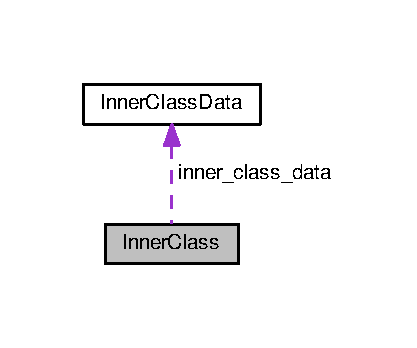
\includegraphics[width=200pt]{class_inner_class__coll__graph}
\end{center}
\end{figure}
\subsection*{Componentes}
\begin{DoxyCompactItemize}
\item 
class \hyperlink{class_inner_class_1_1print}{print}
\begin{DoxyCompactList}\small\item\em Print do tamanho da class;. \end{DoxyCompactList}\item 
class \hyperlink{class_inner_class_1_1read}{read}
\begin{DoxyCompactList}\small\item\em Leitura do tamanho da Class;. \end{DoxyCompactList}\end{DoxyCompactItemize}
\subsection*{Membros públicos}
\begin{DoxyCompactItemize}
\item 
void \hyperlink{class_inner_class_ab178cb43a3277c1ade99a8a0c346cd49}{read} (F\+I\+LE $\ast$)
\item 
void \hyperlink{class_inner_class_acf89443e049952e22a4afeaa43e3bc8c}{print} (std\+::vector$<$ \hyperlink{class_cp_info}{Cp\+Info} $\ast$ $>$)
\end{DoxyCompactItemize}
\subsection*{Atributos Públicos}
\begin{DoxyCompactItemize}
\item 
uint16\+\_\+t \hyperlink{class_inner_class_a7976c7530d97d879907ce035a9b7d2c7}{class\+\_\+length}
\item 
\hyperlink{class_inner_class_data}{Inner\+Class\+Data} $\ast$ \hyperlink{class_inner_class_ad9876452a134d1d5063223610dae7d6a}{inner\+\_\+class\+\_\+data}
\end{DoxyCompactItemize}


\subsection{Descrição detalhada}
classe contém class\+\_\+length e ponteiro para inner\+\_\+class\+\_\+data -\/ todos uint16; Além disso contém metodos como read e print 

\subsection{Documentação dos métodos}
\index{Inner\+Class@{Inner\+Class}!print@{print}}
\index{print@{print}!Inner\+Class@{Inner\+Class}}
\subsubsection[{\texorpdfstring{print(std\+::vector$<$ Cp\+Info $\ast$ $>$)}{print(std::vector< CpInfo * >)}}]{\setlength{\rightskip}{0pt plus 5cm}void {\bf Inner\+Class\+::print} (
\begin{DoxyParamCaption}
\item[{std\+::vector$<$ {\bf Cp\+Info} $\ast$ $>$}]{true\+Cp\+Info}
\end{DoxyParamCaption}
)}\hypertarget{class_inner_class_acf89443e049952e22a4afeaa43e3bc8c}{}\label{class_inner_class_acf89443e049952e22a4afeaa43e3bc8c}
\index{Inner\+Class@{Inner\+Class}!read@{read}}
\index{read@{read}!Inner\+Class@{Inner\+Class}}
\subsubsection[{\texorpdfstring{read(\+F\+I\+L\+E $\ast$)}{read(FILE *)}}]{\setlength{\rightskip}{0pt plus 5cm}void {\bf Inner\+Class\+::read} (
\begin{DoxyParamCaption}
\item[{F\+I\+LE $\ast$}]{fp}
\end{DoxyParamCaption}
)}\hypertarget{class_inner_class_ab178cb43a3277c1ade99a8a0c346cd49}{}\label{class_inner_class_ab178cb43a3277c1ade99a8a0c346cd49}


Grafo de chamadas desta função\+:
\nopagebreak
\begin{figure}[H]
\begin{center}
\leavevmode
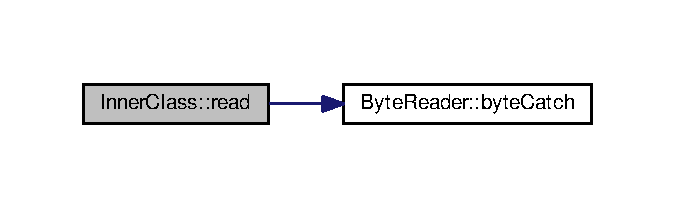
\includegraphics[width=324pt]{class_inner_class_ab178cb43a3277c1ade99a8a0c346cd49_cgraph}
\end{center}
\end{figure}




\subsection{Documentação dos dados membro}
\index{Inner\+Class@{Inner\+Class}!class\+\_\+length@{class\+\_\+length}}
\index{class\+\_\+length@{class\+\_\+length}!Inner\+Class@{Inner\+Class}}
\subsubsection[{\texorpdfstring{class\+\_\+length}{class_length}}]{\setlength{\rightskip}{0pt plus 5cm}uint16\+\_\+t Inner\+Class\+::class\+\_\+length}\hypertarget{class_inner_class_a7976c7530d97d879907ce035a9b7d2c7}{}\label{class_inner_class_a7976c7530d97d879907ce035a9b7d2c7}
\index{Inner\+Class@{Inner\+Class}!inner\+\_\+class\+\_\+data@{inner\+\_\+class\+\_\+data}}
\index{inner\+\_\+class\+\_\+data@{inner\+\_\+class\+\_\+data}!Inner\+Class@{Inner\+Class}}
\subsubsection[{\texorpdfstring{inner\+\_\+class\+\_\+data}{inner_class_data}}]{\setlength{\rightskip}{0pt plus 5cm}{\bf Inner\+Class\+Data}$\ast$ Inner\+Class\+::inner\+\_\+class\+\_\+data}\hypertarget{class_inner_class_ad9876452a134d1d5063223610dae7d6a}{}\label{class_inner_class_ad9876452a134d1d5063223610dae7d6a}


A documentação para esta classe foi gerada a partir dos seguintes ficheiros\+:\begin{DoxyCompactItemize}
\item 
\hyperlink{_attribute_info_8hpp}{Attribute\+Info.\+hpp}\item 
\hyperlink{_attribute_info_8cpp}{Attribute\+Info.\+cpp}\end{DoxyCompactItemize}

\hypertarget{class_inner_class_data}{}\section{Inner\+Class\+Data Class Reference}
\label{class_inner_class_data}\index{Inner\+Class\+Data@{Inner\+Class\+Data}}


classe contém inner\+\_\+class\+\_\+info\+\_\+index, outer\+\_\+class\+\_\+info\+\_\+index, inner\+\_\+name\+\_\+index e inner\+\_\+class\+\_\+access\+\_\+flag;  




{\ttfamily \#include $<$Attribute\+Info.\+hpp$>$}

\subsection*{Public Attributes}
\begin{DoxyCompactItemize}
\item 
uint16\+\_\+t \hyperlink{class_inner_class_data_a58436b7ecd12950e542f64ee18906c59}{inner\+\_\+class\+\_\+info\+\_\+index}
\item 
uint16\+\_\+t \hyperlink{class_inner_class_data_a0370a0b4e7adc2b2524979040dc52f9d}{outer\+\_\+class\+\_\+info\+\_\+index}
\item 
uint16\+\_\+t \hyperlink{class_inner_class_data_af11ac765a0638f41283f42eb51b9064a}{inner\+\_\+name\+\_\+index}
\item 
uint16\+\_\+t \hyperlink{class_inner_class_data_a4c52c10364307d7be48aac8f7a5d88ed}{inner\+\_\+class\+\_\+access\+\_\+flag}
\end{DoxyCompactItemize}


\subsection{Detailed Description}
classe contém inner\+\_\+class\+\_\+info\+\_\+index, outer\+\_\+class\+\_\+info\+\_\+index, inner\+\_\+name\+\_\+index e inner\+\_\+class\+\_\+access\+\_\+flag; 

\subsection{Member Data Documentation}
\index{Inner\+Class\+Data@{Inner\+Class\+Data}!inner\+\_\+class\+\_\+access\+\_\+flag@{inner\+\_\+class\+\_\+access\+\_\+flag}}
\index{inner\+\_\+class\+\_\+access\+\_\+flag@{inner\+\_\+class\+\_\+access\+\_\+flag}!Inner\+Class\+Data@{Inner\+Class\+Data}}
\subsubsection[{\texorpdfstring{inner\+\_\+class\+\_\+access\+\_\+flag}{inner_class_access_flag}}]{\setlength{\rightskip}{0pt plus 5cm}uint16\+\_\+t Inner\+Class\+Data\+::inner\+\_\+class\+\_\+access\+\_\+flag}\hypertarget{class_inner_class_data_a4c52c10364307d7be48aac8f7a5d88ed}{}\label{class_inner_class_data_a4c52c10364307d7be48aac8f7a5d88ed}
\index{Inner\+Class\+Data@{Inner\+Class\+Data}!inner\+\_\+class\+\_\+info\+\_\+index@{inner\+\_\+class\+\_\+info\+\_\+index}}
\index{inner\+\_\+class\+\_\+info\+\_\+index@{inner\+\_\+class\+\_\+info\+\_\+index}!Inner\+Class\+Data@{Inner\+Class\+Data}}
\subsubsection[{\texorpdfstring{inner\+\_\+class\+\_\+info\+\_\+index}{inner_class_info_index}}]{\setlength{\rightskip}{0pt plus 5cm}uint16\+\_\+t Inner\+Class\+Data\+::inner\+\_\+class\+\_\+info\+\_\+index}\hypertarget{class_inner_class_data_a58436b7ecd12950e542f64ee18906c59}{}\label{class_inner_class_data_a58436b7ecd12950e542f64ee18906c59}
\index{Inner\+Class\+Data@{Inner\+Class\+Data}!inner\+\_\+name\+\_\+index@{inner\+\_\+name\+\_\+index}}
\index{inner\+\_\+name\+\_\+index@{inner\+\_\+name\+\_\+index}!Inner\+Class\+Data@{Inner\+Class\+Data}}
\subsubsection[{\texorpdfstring{inner\+\_\+name\+\_\+index}{inner_name_index}}]{\setlength{\rightskip}{0pt plus 5cm}uint16\+\_\+t Inner\+Class\+Data\+::inner\+\_\+name\+\_\+index}\hypertarget{class_inner_class_data_af11ac765a0638f41283f42eb51b9064a}{}\label{class_inner_class_data_af11ac765a0638f41283f42eb51b9064a}
\index{Inner\+Class\+Data@{Inner\+Class\+Data}!outer\+\_\+class\+\_\+info\+\_\+index@{outer\+\_\+class\+\_\+info\+\_\+index}}
\index{outer\+\_\+class\+\_\+info\+\_\+index@{outer\+\_\+class\+\_\+info\+\_\+index}!Inner\+Class\+Data@{Inner\+Class\+Data}}
\subsubsection[{\texorpdfstring{outer\+\_\+class\+\_\+info\+\_\+index}{outer_class_info_index}}]{\setlength{\rightskip}{0pt plus 5cm}uint16\+\_\+t Inner\+Class\+Data\+::outer\+\_\+class\+\_\+info\+\_\+index}\hypertarget{class_inner_class_data_a0370a0b4e7adc2b2524979040dc52f9d}{}\label{class_inner_class_data_a0370a0b4e7adc2b2524979040dc52f9d}


The documentation for this class was generated from the following file\+:\begin{DoxyCompactItemize}
\item 
\hyperlink{_attribute_info_8hpp}{Attribute\+Info.\+hpp}\end{DoxyCompactItemize}

\hypertarget{class_instruction_impl_1_1ins__goto}{}\section{Referência à classe Instruction\+Impl\+:\+:ins\+\_\+goto}
\label{class_instruction_impl_1_1ins__goto}\index{Instruction\+Impl\+::ins\+\_\+goto@{Instruction\+Impl\+::ins\+\_\+goto}}


Realiza um falto baseado em um offset.  




\subsection{Descrição detalhada}
Realiza um falto baseado em um offset. 


\begin{DoxyParams}{Parâmetros}
{\em $\ast$this\+\_\+frame} & ponteiro para o frame atual.  \\
\hline
\end{DoxyParams}


A documentação para esta classe foi gerada a partir do seguinte ficheiro\+:\begin{DoxyCompactItemize}
\item 
\hyperlink{_instruction_impl_8cpp}{Instruction\+Impl.\+cpp}\end{DoxyCompactItemize}

\hypertarget{class_instance_1_1_instance}{}\section{Instance\+:\+:Instance Class Reference}
\label{class_instance_1_1_instance}\index{Instance\+::\+Instance@{Instance\+::\+Instance}}


Carrega as informações de um \hyperlink{class_class_loader}{Class\+Loader} na Instancia.  




\subsection{Detailed Description}
Carrega as informações de um \hyperlink{class_class_loader}{Class\+Loader} na Instancia. 


\begin{DoxyParams}{Parameters}
{\em $\ast$to\+Load} & ponteiro para \hyperlink{class_class_loader}{Class\+Loader}. \\
\hline
\end{DoxyParams}
\begin{DoxyReturn}{Returns}
constructor 
\end{DoxyReturn}


The documentation for this class was generated from the following file\+:\begin{DoxyCompactItemize}
\item 
\hyperlink{_instance_8cpp}{Instance.\+cpp}\end{DoxyCompactItemize}

\hypertarget{struct_instance}{}\section{Instance Struct Reference}
\label{struct_instance}\index{Instance@{Instance}}


tipo que determinará o nome e o tipo de operando através do \hyperlink{struct_operand}{Operand} class; Álém contém o método \hyperlink{class_instance_1_1_instance}{Instance\+::\+Instance}  




{\ttfamily \#include $<$Instance.\+hpp$>$}



Collaboration diagram for Instance\+:
% FIG 0
\subsection*{Classes}
\begin{DoxyCompactItemize}
\item 
class \hyperlink{class_instance_1_1_instance}{Instance}
\begin{DoxyCompactList}\small\item\em Carrega as informações de um \hyperlink{class_class_loader}{Class\+Loader} na Instancia. \end{DoxyCompactList}\end{DoxyCompactItemize}
\subsection*{Public Member Functions}
\begin{DoxyCompactItemize}
\item 
\hyperlink{struct_instance_aca86b4cbc971ace708021f8ef2c6ce43}{Instance} (\hyperlink{class_class_loader}{Class\+Loader} $\ast$)
\end{DoxyCompactItemize}
\subsection*{Public Attributes}
\begin{DoxyCompactItemize}
\item 
std\+::string \hyperlink{struct_instance_a80e29939a8dac12ad5d8008f3df241af}{name}
\item 
std\+::map$<$ std\+::string, \hyperlink{struct_operand}{Operand} $\ast$ $>$ $\ast$ \hyperlink{struct_instance_a3262e6460c3b4fa873a3a439e77fdf7e}{references}
\item 
\hyperlink{class_class_loader}{Class\+Loader} $\ast$ \hyperlink{struct_instance_a7247d0aa8380ec112069ad6c78a11bd2}{classe}
\end{DoxyCompactItemize}


\subsection{Detailed Description}
tipo que determinará o nome e o tipo de operando através do \hyperlink{struct_operand}{Operand} class; Álém contém o método \hyperlink{class_instance_1_1_instance}{Instance\+::\+Instance} 

\subsection{Constructor \& Destructor Documentation}
\index{Instance@{Instance}!Instance@{Instance}}
\index{Instance@{Instance}!Instance@{Instance}}
\subsubsection[{\texorpdfstring{Instance(\+Class\+Loader $\ast$)}{Instance(ClassLoader *)}}]{\setlength{\rightskip}{0pt plus 5cm}{\bf Instance\+::\+Instance} (
\begin{DoxyParamCaption}
\item[{{\bf Class\+Loader} $\ast$}]{to\+Load}
\end{DoxyParamCaption}
)}\hypertarget{struct_instance_aca86b4cbc971ace708021f8ef2c6ce43}{}\label{struct_instance_aca86b4cbc971ace708021f8ef2c6ce43}


Here is the call graph for this function\+:
% FIG 1




\subsection{Member Data Documentation}
\index{Instance@{Instance}!classe@{classe}}
\index{classe@{classe}!Instance@{Instance}}
\subsubsection[{\texorpdfstring{classe}{classe}}]{\setlength{\rightskip}{0pt plus 5cm}{\bf Class\+Loader}$\ast$ Instance\+::classe}\hypertarget{struct_instance_a7247d0aa8380ec112069ad6c78a11bd2}{}\label{struct_instance_a7247d0aa8380ec112069ad6c78a11bd2}
\index{Instance@{Instance}!name@{name}}
\index{name@{name}!Instance@{Instance}}
\subsubsection[{\texorpdfstring{name}{name}}]{\setlength{\rightskip}{0pt plus 5cm}std\+::string Instance\+::name}\hypertarget{struct_instance_a80e29939a8dac12ad5d8008f3df241af}{}\label{struct_instance_a80e29939a8dac12ad5d8008f3df241af}
\index{Instance@{Instance}!references@{references}}
\index{references@{references}!Instance@{Instance}}
\subsubsection[{\texorpdfstring{references}{references}}]{\setlength{\rightskip}{0pt plus 5cm}std\+::map$<$ std\+::string, {\bf Operand}$\ast$ $>$$\ast$ Instance\+::references}\hypertarget{struct_instance_a3262e6460c3b4fa873a3a439e77fdf7e}{}\label{struct_instance_a3262e6460c3b4fa873a3a439e77fdf7e}


The documentation for this struct was generated from the following files\+:\begin{DoxyCompactItemize}
\item 
\hyperlink{_instance_8hpp}{Instance.\+hpp}\item 
\hyperlink{_instance_8cpp}{Instance.\+cpp}\end{DoxyCompactItemize}

\hypertarget{class_instruction_impl_1_1instanceof}{}\section{Instruction\+Impl\+:\+:instanceof Class Reference}
\label{class_instruction_impl_1_1instanceof}\index{Instruction\+Impl\+::instanceof@{Instruction\+Impl\+::instanceof}}


Verifica se o objeto é do tipo dado.  




\subsection{Detailed Description}
Verifica se o objeto é do tipo dado. 


\begin{DoxyParams}{Parameters}
{\em $\ast$this\+\_\+frame} & ponteiro para o frame atual \\
\hline
\end{DoxyParams}
\begin{DoxyReturn}{Returns}
void 
\end{DoxyReturn}


The documentation for this class was generated from the following file\+:\begin{DoxyCompactItemize}
\item 
\hyperlink{_instruction_impl_8cpp}{Instruction\+Impl.\+cpp}\end{DoxyCompactItemize}

\hypertarget{class_instruction}{}\section{Referência à classe Instruction}
\label{class_instruction}\index{Instruction@{Instruction}}


Determina a instrução de acordo com o interpretador;.  




{\ttfamily \#include $<$Instruction.\+hpp$>$}

\subsection*{Componentes}
\begin{DoxyCompactItemize}
\item 
class \hyperlink{class_instruction_1_1init}{init}
\begin{DoxyCompactList}\small\item\em Inilizar todas as instruções em uma array para facilitar o mapeamento;. \end{DoxyCompactList}\end{DoxyCompactItemize}
\subsection*{Membros públicos estáticos}
\begin{DoxyCompactItemize}
\item 
static void \hyperlink{class_instruction_a145a172552303c9cbd8a5856e31a701b}{init} (\hyperlink{class_instruction}{Instruction} $\ast$)
\end{DoxyCompactItemize}
\subsection*{Atributos Públicos}
\begin{DoxyCompactItemize}
\item 
std\+::string \hyperlink{class_instruction_abfd1615a8bb140e70b3724214deee7df}{name}
\item 
uint32\+\_\+t \hyperlink{class_instruction_a1052c075af597277407bece6db3f2bef}{bytes}
\item 
void($\ast$ \hyperlink{class_instruction_a1f4648eed807151537ef72c78d65081f}{func} )(\hyperlink{struct_frame}{Frame} $\ast$this\+\_\+frame)
\end{DoxyCompactItemize}


\subsection{Descrição detalhada}
Determina a instrução de acordo com o interpretador;. 

\subsection{Documentação dos métodos}
\index{Instruction@{Instruction}!init@{init}}
\index{init@{init}!Instruction@{Instruction}}
\subsubsection[{\texorpdfstring{init(\+Instruction $\ast$)}{init(Instruction *)}}]{\setlength{\rightskip}{0pt plus 5cm}void {\bf Instruction\+::init} (
\begin{DoxyParamCaption}
\item[{{\bf Instruction} $\ast$}]{instructions}
\end{DoxyParamCaption}
)\hspace{0.3cm}{\ttfamily [static]}}\hypertarget{class_instruction_a145a172552303c9cbd8a5856e31a701b}{}\label{class_instruction_a145a172552303c9cbd8a5856e31a701b}


Este é o diagrama das funções que utilizam esta função\+:
\nopagebreak
\begin{figure}[H]
\begin{center}
\leavevmode
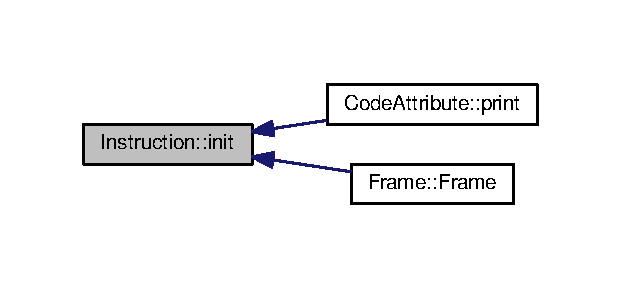
\includegraphics[width=298pt]{class_instruction_a145a172552303c9cbd8a5856e31a701b_icgraph}
\end{center}
\end{figure}




\subsection{Documentação dos dados membro}
\index{Instruction@{Instruction}!bytes@{bytes}}
\index{bytes@{bytes}!Instruction@{Instruction}}
\subsubsection[{\texorpdfstring{bytes}{bytes}}]{\setlength{\rightskip}{0pt plus 5cm}uint32\+\_\+t Instruction\+::bytes}\hypertarget{class_instruction_a1052c075af597277407bece6db3f2bef}{}\label{class_instruction_a1052c075af597277407bece6db3f2bef}
\index{Instruction@{Instruction}!func@{func}}
\index{func@{func}!Instruction@{Instruction}}
\subsubsection[{\texorpdfstring{func}{func}}]{\setlength{\rightskip}{0pt plus 5cm}void($\ast$  Instruction\+::func) ({\bf Frame} $\ast$this\+\_\+frame)}\hypertarget{class_instruction_a1f4648eed807151537ef72c78d65081f}{}\label{class_instruction_a1f4648eed807151537ef72c78d65081f}
\index{Instruction@{Instruction}!name@{name}}
\index{name@{name}!Instruction@{Instruction}}
\subsubsection[{\texorpdfstring{name}{name}}]{\setlength{\rightskip}{0pt plus 5cm}std\+::string Instruction\+::name}\hypertarget{class_instruction_abfd1615a8bb140e70b3724214deee7df}{}\label{class_instruction_abfd1615a8bb140e70b3724214deee7df}


A documentação para esta classe foi gerada a partir dos seguintes ficheiros\+:\begin{DoxyCompactItemize}
\item 
\hyperlink{_instruction_8hpp}{Instruction.\+hpp}\item 
\hyperlink{_instruction_8cpp}{Instruction.\+cpp}\end{DoxyCompactItemize}

\hypertarget{class_instruction_impl}{}\section{Instruction\+Impl Class Reference}
\label{class_instruction_impl}\index{Instruction\+Impl@{Instruction\+Impl}}


Objetivo incluir todos os metodos para a ação de cada instrução achada pelo interpretador;.  




{\ttfamily \#include $<$Instruction\+Impl.\+hpp$>$}

\subsection*{Classes}
\begin{DoxyCompactItemize}
\item 
class \hyperlink{class_instruction_impl_1_1aaload}{aaload}
\begin{DoxyCompactList}\small\item\em retorna uma referência a um objeto, contido em um array de objetos e coloca tal referência na stack \end{DoxyCompactList}\item 
class \hyperlink{class_instruction_impl_1_1aastore}{aastore}
\begin{DoxyCompactList}\small\item\em Desempilha a referencia para o array, o indice e o valor(referencia) e salva o valor no array. \end{DoxyCompactList}\item 
class \hyperlink{class_instruction_impl_1_1aconst__null}{aconst\+\_\+null}
\begin{DoxyCompactList}\small\item\em Empilha uma referência nula a um objeto na pilha de operandos. \end{DoxyCompactList}\item 
class \hyperlink{class_instruction_impl_1_1aload__0}{aload\+\_\+0}
\begin{DoxyCompactList}\small\item\em Uma referencia do objeto na posicao 0 do vetor de variaveis locais é colocada na pilha de operandos. \end{DoxyCompactList}\item 
class \hyperlink{class_instruction_impl_1_1aload__1}{aload\+\_\+1}
\begin{DoxyCompactList}\small\item\em Uma referencia do objeto na posicao 1 do vetor de variaveis locais é colocada na pilha de operandos. \end{DoxyCompactList}\item 
class \hyperlink{class_instruction_impl_1_1aload__2}{aload\+\_\+2}
\begin{DoxyCompactList}\small\item\em Uma referencia do objeto na posicao 2 do vetor de variaveis locais é colocada na pilha de operandos. \end{DoxyCompactList}\item 
class \hyperlink{class_instruction_impl_1_1aload__3}{aload\+\_\+3}
\begin{DoxyCompactList}\small\item\em Uma referencia do objeto na posicao 3 do vetor de variaveis locais é colocada na pilha de operandos. \end{DoxyCompactList}\item 
class \hyperlink{class_instruction_impl_1_1anewarray}{anewarray}
\begin{DoxyCompactList}\small\item\em Criar um novo array de referência. \end{DoxyCompactList}\item 
class \hyperlink{class_instruction_impl_1_1areturn}{areturn}
\begin{DoxyCompactList}\small\item\em retorna um objeto para o frame anterior. \end{DoxyCompactList}\item 
class \hyperlink{class_instruction_impl_1_1arraylength}{arraylength}
\begin{DoxyCompactList}\small\item\em pega a referencia de um array, remove array, e empilha o seu tamanho no lugar \end{DoxyCompactList}\item 
class \hyperlink{class_instruction_impl_1_1astore}{astore}
\begin{DoxyCompactList}\small\item\em Armazena uma referencia de objeto no array de variaveis locais no valor indicado pelo indice. \end{DoxyCompactList}\item 
class \hyperlink{class_instruction_impl_1_1astore__0}{astore\+\_\+0}
\begin{DoxyCompactList}\small\item\em Guarda um objeto em uma na posição 0 do vetor de variáveis. \end{DoxyCompactList}\item 
class \hyperlink{class_instruction_impl_1_1astore__1}{astore\+\_\+1}
\begin{DoxyCompactList}\small\item\em desempilha um operando do topo da pilha de operandos, guardando sua referência do array de variáveis locais na posiçao 1 \end{DoxyCompactList}\item 
class \hyperlink{class_instruction_impl_1_1astore__2}{astore\+\_\+2}
\begin{DoxyCompactList}\small\item\em desempilha um operando do topo da pilha de operandos, guardando sua referência do array de variáveis locais na posiçao 2 \end{DoxyCompactList}\item 
class \hyperlink{class_instruction_impl_1_1astore__3}{astore\+\_\+3}
\begin{DoxyCompactList}\small\item\em desempilha um operando do topo da pilha de operandos, guardando sua referência do array de variáveis locais na posiçao 3 \end{DoxyCompactList}\item 
class \hyperlink{class_instruction_impl_1_1athrow}{athrow}
\begin{DoxyCompactList}\small\item\em Jogar um erro de exceção. \end{DoxyCompactList}\item 
class \hyperlink{class_instruction_impl_1_1baload}{baload}
\begin{DoxyCompactList}\small\item\em Empilha na pilha de operandos um byte de um array de bytes. \end{DoxyCompactList}\item 
class \hyperlink{class_instruction_impl_1_1bastore}{bastore}
\begin{DoxyCompactList}\small\item\em Desempilha a referencia para o array, o indice e o valor(byte) e salva o valor no array. \end{DoxyCompactList}\item 
class \hyperlink{class_instruction_impl_1_1bipush}{bipush}
\begin{DoxyCompactList}\small\item\em Empilha na pilha de operandos um inteiro composto por um byte encontrado no em this\+\_\+frame-\/$>$method\+\_\+code.\+code. \end{DoxyCompactList}\item 
class \hyperlink{class_instruction_impl_1_1caload}{caload}
\begin{DoxyCompactList}\small\item\em Empilha na pilha de operandos um char de um array de chars. \end{DoxyCompactList}\item 
class \hyperlink{class_instruction_impl_1_1castore}{castore}
\begin{DoxyCompactList}\small\item\em Desempilha a referencia para o array, o indice e o valor(char) e salva o valor no array. Trunca inteiro de 32 bits da pilha para 16 bits. \end{DoxyCompactList}\item 
class \hyperlink{class_instruction_impl_1_1checkcast}{checkcast}
\begin{DoxyCompactList}\small\item\em Verifica se o objeto é do tipo dado. \end{DoxyCompactList}\item 
class \hyperlink{class_instruction_impl_1_1d2f}{d2f}
\begin{DoxyCompactList}\small\item\em Converte de double para float. \end{DoxyCompactList}\item 
class \hyperlink{class_instruction_impl_1_1d2i}{d2i}
\begin{DoxyCompactList}\small\item\em Função que desempilha um double, converte para inteiro e empilha novamente. \end{DoxyCompactList}\item 
class \hyperlink{class_instruction_impl_1_1d2l}{d2l}
\begin{DoxyCompactList}\small\item\em Converte de double para long. \end{DoxyCompactList}\item 
class \hyperlink{class_instruction_impl_1_1dadd}{dadd}
\begin{DoxyCompactList}\small\item\em Desempilha 2 doubles da pilha de operandos e empilha a soma deles. \end{DoxyCompactList}\item 
class \hyperlink{class_instruction_impl_1_1daload}{daload}
\begin{DoxyCompactList}\small\item\em Empilha na pilha de operandos um elemento de um array de float de dupla precisao. \end{DoxyCompactList}\item 
class \hyperlink{class_instruction_impl_1_1dastore}{dastore}
\begin{DoxyCompactList}\small\item\em Guarda em uma double array. \end{DoxyCompactList}\item 
class \hyperlink{class_instruction_impl_1_1dcmpg}{dcmpg}
\begin{DoxyCompactList}\small\item\em Função desempilha dois doubles, compara os memos e empilha o resultado da comparação. 0 se forem iguais, se o segundo número for maior empilha 1, caso contrário empilha -\/1. Caso algum dos números seja NaN, empilha 1. \end{DoxyCompactList}\item 
class \hyperlink{class_instruction_impl_1_1dcmpl}{dcmpl}
\begin{DoxyCompactList}\small\item\em Função desempilha dois doubles, compara os memos e empilha o resultado da comparação. 0 se forem iguais, se o segundo número for maior empilha 1, caso contrário empilha -\/1. Caso algum dos números seja NaN, empilha 0. \end{DoxyCompactList}\item 
class \hyperlink{class_instruction_impl_1_1dconst__0}{dconst\+\_\+0}
\begin{DoxyCompactList}\small\item\em Empilha a constante double 0.\+0 na pilha de operandos. \end{DoxyCompactList}\item 
class \hyperlink{class_instruction_impl_1_1dconst__1}{dconst\+\_\+1}
\begin{DoxyCompactList}\small\item\em Empilha a constante double 1.\+0 na pilha de operandos. \end{DoxyCompactList}\item 
class \hyperlink{class_instruction_impl_1_1ddiv}{ddiv}
\begin{DoxyCompactList}\small\item\em Desempilha 2 doubles da pilha de operandos e empilha a divisão deles. \end{DoxyCompactList}\item 
class \hyperlink{class_instruction_impl_1_1dload}{dload}
\begin{DoxyCompactList}\small\item\em Dá push em um valor de preciso dupla de uma variável local para a pilha de operandos. \end{DoxyCompactList}\item 
class \hyperlink{class_instruction_impl_1_1dload__0}{dload\+\_\+0}
\begin{DoxyCompactList}\small\item\em empilha double indicado no indice 0 do array de variaveis locais na pilha de operandos \end{DoxyCompactList}\item 
class \hyperlink{class_instruction_impl_1_1dload__1}{dload\+\_\+1}
\begin{DoxyCompactList}\small\item\em empilha double indicado no indice 1 do array de variaveis locais na pilha de operandos \end{DoxyCompactList}\item 
class \hyperlink{class_instruction_impl_1_1dload__2}{dload\+\_\+2}
\begin{DoxyCompactList}\small\item\em empilha double indicado no indice 2 do array de variaveis locais na pilha de operandos \end{DoxyCompactList}\item 
class \hyperlink{class_instruction_impl_1_1dload__3}{dload\+\_\+3}
\begin{DoxyCompactList}\small\item\em empilha double indicado no indice 3 do array de variaveis locais na pilha de operandos \end{DoxyCompactList}\item 
class \hyperlink{class_instruction_impl_1_1dmul}{dmul}
\begin{DoxyCompactList}\small\item\em Desempilha 2 doubles da pilha de operandos e empilha a produto deles. \end{DoxyCompactList}\item 
class \hyperlink{class_instruction_impl_1_1dneg}{dneg}
\begin{DoxyCompactList}\small\item\em Desempilha 1 doubles da pilha de operandos e empilha o valor negativo dele. \end{DoxyCompactList}\item 
class \hyperlink{class_instruction_impl_1_1drem}{drem}
\begin{DoxyCompactList}\small\item\em Desempilha dois doubles da pilha e empilha resto da divisão entre eles. \end{DoxyCompactList}\item 
class \hyperlink{class_instruction_impl_1_1dreturn}{dreturn}
\begin{DoxyCompactList}\small\item\em Retorna double de um método. \end{DoxyCompactList}\item 
class \hyperlink{class_instruction_impl_1_1dstore}{dstore}
\begin{DoxyCompactList}\small\item\em Armazena valor double da pilha de operandos no array de variaveis locais no indice index. \end{DoxyCompactList}\item 
class \hyperlink{class_instruction_impl_1_1dstore__0}{dstore\+\_\+0}
\begin{DoxyCompactList}\small\item\em Armazena valor double da pilha de operandos no array de variaveis locais no indice 0. \end{DoxyCompactList}\item 
class \hyperlink{class_instruction_impl_1_1dstore__1}{dstore\+\_\+1}
\begin{DoxyCompactList}\small\item\em Armazena valor double da pilha de operandos no array de variaveis locais no indice 1. \end{DoxyCompactList}\item 
class \hyperlink{class_instruction_impl_1_1dstore__2}{dstore\+\_\+2}
\begin{DoxyCompactList}\small\item\em Armazena valor double da pilha de operandos no array de variaveis locais no indice 2. \end{DoxyCompactList}\item 
class \hyperlink{class_instruction_impl_1_1dstore__3}{dstore\+\_\+3}
\begin{DoxyCompactList}\small\item\em Armazena valor double da pilha de operandos no array de variaveis locais no indice 3. \end{DoxyCompactList}\item 
class \hyperlink{class_instruction_impl_1_1dsub}{dsub}
\begin{DoxyCompactList}\small\item\em Desempilha 2 doubles da pilha de operandos e empilha a subtração deles. \end{DoxyCompactList}\item 
class \hyperlink{class_instruction_impl_1_1dup}{dup}
\begin{DoxyCompactList}\small\item\em Duplica um valor da pilha de operandos e insere os valores duplicados na ordem original. \end{DoxyCompactList}\item 
class \hyperlink{class_instruction_impl_1_1dup2}{dup2}
\begin{DoxyCompactList}\small\item\em Duplica um ou dois valores da pilha de operandos e insere os valores duplicados na ordem original. \end{DoxyCompactList}\item 
class \hyperlink{class_instruction_impl_1_1dup2__x1}{dup2\+\_\+x1}
\begin{DoxyCompactList}\small\item\em Duplica os dois primeiro valores da pilha embaixo do penultimo valor da pilha. \end{DoxyCompactList}\item 
class \hyperlink{class_instruction_impl_1_1dup2__x2}{dup2\+\_\+x2}
\begin{DoxyCompactList}\small\item\em Duplica os dois primeiro valores da pilha embaixo do penultimo valor da pilha. \end{DoxyCompactList}\item 
class \hyperlink{class_instruction_impl_1_1dup__x1}{dup\+\_\+x1}
\begin{DoxyCompactList}\small\item\em Realiza uma duplicação b, a -\/$>$ a, b, a. \end{DoxyCompactList}\item 
class \hyperlink{class_instruction_impl_1_1dup__x2}{dup\+\_\+x2}
\begin{DoxyCompactList}\small\item\em Duplica os valores do topo da pilha de operandos e insere dois ou três valores abaixo. \end{DoxyCompactList}\item 
class \hyperlink{class_instruction_impl_1_1f2d}{f2d}
\begin{DoxyCompactList}\small\item\em Desempilha 1 float da pilha de operandos e o converte para double e empilha o resultado na pilha de operandos. \end{DoxyCompactList}\item 
class \hyperlink{class_instruction_impl_1_1f2i}{f2i}
\begin{DoxyCompactList}\small\item\em Desempilha 1 float da pilha de operandos e o converte para inteiro e empilha o resultado na pilha de operandos. \end{DoxyCompactList}\item 
class \hyperlink{class_instruction_impl_1_1f2l}{f2l}
\begin{DoxyCompactList}\small\item\em converte float para long \end{DoxyCompactList}\item 
class \hyperlink{class_instruction_impl_1_1fadd}{fadd}
\begin{DoxyCompactList}\small\item\em Desempilha dois float da pilha e empilha adição deles. \end{DoxyCompactList}\item 
class \hyperlink{class_instruction_impl_1_1faload}{faload}
\begin{DoxyCompactList}\small\item\em Empilha na pilha de operandos um elemento de um array de float. \end{DoxyCompactList}\item 
class \hyperlink{class_instruction_impl_1_1fastore}{fastore}
\begin{DoxyCompactList}\small\item\em Desempilha a referencia para o array, o indice e o valor(float) e salva o valor no array. \end{DoxyCompactList}\item 
class \hyperlink{class_instruction_impl_1_1fcmpg}{fcmpg}
\begin{DoxyCompactList}\small\item\em Função desempilha dois floats, compara ambos e empilha o resultado da comparação. Se são iguais empilha 0, se o segundo número for maior empilha 1, caso contrário empilha -\/1. Caso algum dos números seja NaN, empilha 1. \end{DoxyCompactList}\item 
class \hyperlink{class_instruction_impl_1_1fcmpl}{fcmpl}
\begin{DoxyCompactList}\small\item\em Função que desempilha dois floats, compara ambos e empilha o resultado da comparação. 0 se forem iguais, se o segundo número for maior empilha 1, caso contrário empilha -\/1. Caso algum dos números seja NaN, empilha 1. \end{DoxyCompactList}\item 
class \hyperlink{class_instruction_impl_1_1fconst__0}{fconst\+\_\+0}
\begin{DoxyCompactList}\small\item\em Empilha a constante float 0.\+0 na pilha de operandos. \end{DoxyCompactList}\item 
class \hyperlink{class_instruction_impl_1_1fconst__1}{fconst\+\_\+1}
\begin{DoxyCompactList}\small\item\em Empilha a constante float 1.\+0 na pilha de operandos. \end{DoxyCompactList}\item 
class \hyperlink{class_instruction_impl_1_1fconst__2}{fconst\+\_\+2}
\begin{DoxyCompactList}\small\item\em Empilha a constante float 2.\+0 na pilha de operandos. \end{DoxyCompactList}\item 
class \hyperlink{class_instruction_impl_1_1fdiv}{fdiv}
\begin{DoxyCompactList}\small\item\em Desempilha dois floats da pilha e empilha a divisão deles. \end{DoxyCompactList}\item 
class \hyperlink{class_instruction_impl_1_1fload}{fload}
\begin{DoxyCompactList}\small\item\em Empilha float indicado no indice determinado do array de variáveis locais na pilha de operandos. \end{DoxyCompactList}\item 
class \hyperlink{class_instruction_impl_1_1fload__0}{fload\+\_\+0}
\begin{DoxyCompactList}\small\item\em Empilha float indicado no indice 0 do array de variáveis locais na pilha de operandos. \end{DoxyCompactList}\item 
class \hyperlink{class_instruction_impl_1_1fload__1}{fload\+\_\+1}
\begin{DoxyCompactList}\small\item\em Empilha float indicado no indice 1 do array de variáveis locais na pilha de operandos. \end{DoxyCompactList}\item 
class \hyperlink{class_instruction_impl_1_1fload__2}{fload\+\_\+2}
\begin{DoxyCompactList}\small\item\em Empilha float indicado no indice 2 do array de variáveis locais na pilha de operandos. \end{DoxyCompactList}\item 
class \hyperlink{class_instruction_impl_1_1fload__3}{fload\+\_\+3}
\begin{DoxyCompactList}\small\item\em Empilha float indicado no indice 3 do array de variáveis locais na pilha de operandos. \end{DoxyCompactList}\item 
class \hyperlink{class_instruction_impl_1_1fmul}{fmul}
\begin{DoxyCompactList}\small\item\em Desempilha dois floats da pilha e empilha o produto deles. \end{DoxyCompactList}\item 
class \hyperlink{class_instruction_impl_1_1fneg}{fneg}
\begin{DoxyCompactList}\small\item\em Desempilha 1 doubles da pilha de operandos e empilha o valor negativo dele. \end{DoxyCompactList}\item 
class \hyperlink{class_instruction_impl_1_1frem}{frem}
\begin{DoxyCompactList}\small\item\em Desempilha dois floats da pilha e empilha resto da divisão entre eles. \end{DoxyCompactList}\item 
class \hyperlink{class_instruction_impl_1_1freturn}{freturn}
\begin{DoxyCompactList}\small\item\em Retorna float de um método. \end{DoxyCompactList}\item 
class \hyperlink{class_instruction_impl_1_1fstore}{fstore}
\begin{DoxyCompactList}\small\item\em Armazena float do topo da pilha de operandos no array de variaveis locais. \end{DoxyCompactList}\item 
class \hyperlink{class_instruction_impl_1_1fstore__0}{fstore\+\_\+0}
\begin{DoxyCompactList}\small\item\em Armazena float do topo da pilha de operandos no array de variaveis locais no indice 0. \end{DoxyCompactList}\item 
class \hyperlink{class_instruction_impl_1_1fstore__1}{fstore\+\_\+1}
\begin{DoxyCompactList}\small\item\em Armazena float do topo da pilha de operandos no array de variaveis locais no indice 1. \end{DoxyCompactList}\item 
class \hyperlink{class_instruction_impl_1_1fstore__2}{fstore\+\_\+2}
\begin{DoxyCompactList}\small\item\em Armazena float do topo da pilha de operandos no array de variaveis locais no indice 2. \end{DoxyCompactList}\item 
class \hyperlink{class_instruction_impl_1_1fstore__3}{fstore\+\_\+3}
\begin{DoxyCompactList}\small\item\em Armazena float do topo da pilha de operandos no array de variaveis locais no indice 3. \end{DoxyCompactList}\item 
class \hyperlink{class_instruction_impl_1_1fsub}{fsub}
\begin{DoxyCompactList}\small\item\em Desempilha dois floats da pilha e empilha subtração deles. \end{DoxyCompactList}\item 
class \hyperlink{class_instruction_impl_1_1getfield}{getfield}
\begin{DoxyCompactList}\small\item\em Busca o campo de um objeto. \end{DoxyCompactList}\item 
class \hyperlink{class_instruction_impl_1_1getstatic}{getstatic}
\begin{DoxyCompactList}\small\item\em Carrega as classes estáticas na pilha para a execução. \end{DoxyCompactList}\item 
class \hyperlink{class_instruction_impl_1_1goto__w}{goto\+\_\+w}
\begin{DoxyCompactList}\small\item\em Instruçao que executa o desvio para determinado endereco com mais bytes. \end{DoxyCompactList}\item 
class \hyperlink{class_instruction_impl_1_1i2b}{i2b}
\begin{DoxyCompactList}\small\item\em Função convert um inteiro para byte. \end{DoxyCompactList}\item 
class \hyperlink{class_instruction_impl_1_1i2c}{i2c}
\begin{DoxyCompactList}\small\item\em Função que desempilha um inteiro, converte para char e empilha novamente. \end{DoxyCompactList}\item 
class \hyperlink{class_instruction_impl_1_1i2d}{i2d}
\begin{DoxyCompactList}\small\item\em Função que desempilha um inteiro, converte para double e empilha novamente. \end{DoxyCompactList}\item 
class \hyperlink{class_instruction_impl_1_1i2f}{i2f}
\begin{DoxyCompactList}\small\item\em Converte de inteiro para float. \end{DoxyCompactList}\item 
class \hyperlink{class_instruction_impl_1_1i2l}{i2l}
\begin{DoxyCompactList}\small\item\em Função convert operando inteiro long e empilha novamente. \end{DoxyCompactList}\item 
class \hyperlink{class_instruction_impl_1_1i2s}{i2s}
\begin{DoxyCompactList}\small\item\em Função que desempilha um inteiro, converte para short e empilha novamente. \end{DoxyCompactList}\item 
class \hyperlink{class_instruction_impl_1_1i__goto}{i\+\_\+goto}
\begin{DoxyCompactList}\small\item\em Instruçao que executa o desvio para determinado endereco. \end{DoxyCompactList}\item 
class \hyperlink{class_instruction_impl_1_1iadd}{iadd}
\begin{DoxyCompactList}\small\item\em Desempilha 2 inteiros da pilha de operandos e empilha a soma deles. \end{DoxyCompactList}\item 
class \hyperlink{class_instruction_impl_1_1iaload}{iaload}
\begin{DoxyCompactList}\small\item\em Empilha na pilha de operandos um elemento de um array de inteiros. \end{DoxyCompactList}\item 
class \hyperlink{class_instruction_impl_1_1iand}{iand}
\begin{DoxyCompactList}\small\item\em Desempilha dois valores inteiros da pilha, realiza a operação lógica de A\+ND entre os inteiros bit a bit. \end{DoxyCompactList}\item 
class \hyperlink{class_instruction_impl_1_1iastore}{iastore}
\begin{DoxyCompactList}\small\item\em Desempilha a referencia para o array, o indice e o valor(inteiro) e salva o valor no array. \end{DoxyCompactList}\item 
class \hyperlink{class_instruction_impl_1_1iconst__0}{iconst\+\_\+0}
\begin{DoxyCompactList}\small\item\em Empilha 0 na stack de operandos. \end{DoxyCompactList}\item 
class \hyperlink{class_instruction_impl_1_1iconst__1}{iconst\+\_\+1}
\begin{DoxyCompactList}\small\item\em Empilha 1 na stack de operandos. \end{DoxyCompactList}\item 
class \hyperlink{class_instruction_impl_1_1iconst__2}{iconst\+\_\+2}
\begin{DoxyCompactList}\small\item\em Empilha 2 na stack de operandos. \end{DoxyCompactList}\item 
class \hyperlink{class_instruction_impl_1_1iconst__3}{iconst\+\_\+3}
\begin{DoxyCompactList}\small\item\em Empilha 3 na stack de operandos. \end{DoxyCompactList}\item 
class \hyperlink{class_instruction_impl_1_1iconst__4}{iconst\+\_\+4}
\begin{DoxyCompactList}\small\item\em Empilha 4 na stack de operandos. \end{DoxyCompactList}\item 
class \hyperlink{class_instruction_impl_1_1iconst__5}{iconst\+\_\+5}
\begin{DoxyCompactList}\small\item\em Empilha 5 na stack de operandos. \end{DoxyCompactList}\item 
class \hyperlink{class_instruction_impl_1_1iconst__m1}{iconst\+\_\+m1}
\begin{DoxyCompactList}\small\item\em Empilha o inteiro -\/1 na stack de operandos. \end{DoxyCompactList}\item 
class \hyperlink{class_instruction_impl_1_1idiv}{idiv}
\begin{DoxyCompactList}\small\item\em Desempilha dois inteiros da pilha de operandos e empilha o resultado da divisão entre eles. \end{DoxyCompactList}\item 
class \hyperlink{class_instruction_impl_1_1if__acmpeq}{if\+\_\+acmpeq}
\begin{DoxyCompactList}\small\item\em Compara dois objetos e realiza um salto condicional caso obj\+\_\+1 == obj\+\_\+2. \end{DoxyCompactList}\item 
class \hyperlink{class_instruction_impl_1_1if__acmpne}{if\+\_\+acmpne}
\begin{DoxyCompactList}\small\item\em Compara dois objetos e realiza um salto condicional caso obj\+\_\+1 != obj\+\_\+2. \end{DoxyCompactList}\item 
class \hyperlink{class_instruction_impl_1_1if__icmpeq}{if\+\_\+icmpeq}
\begin{DoxyCompactList}\small\item\em Realiza um salto condicional caso o segundo operando na pilha seja == que o topo. \end{DoxyCompactList}\item 
class \hyperlink{class_instruction_impl_1_1if__icmpge}{if\+\_\+icmpge}
\begin{DoxyCompactList}\small\item\em Realiza um salto condicional caso o segundo operando na pilha seja $>$= que o topo. \end{DoxyCompactList}\item 
class \hyperlink{class_instruction_impl_1_1if__icmpgt}{if\+\_\+icmpgt}
\begin{DoxyCompactList}\small\item\em Realiza um salto condicional caso o segundo operando na pilha seja $>$ que o topo. \end{DoxyCompactList}\item 
class \hyperlink{class_instruction_impl_1_1if__icmple}{if\+\_\+icmple}
\begin{DoxyCompactList}\small\item\em Realiza um salto condicional caso o segundo operando na pilha seja $<$= que o topo. \end{DoxyCompactList}\item 
class \hyperlink{class_instruction_impl_1_1if__icmplt}{if\+\_\+icmplt}
\begin{DoxyCompactList}\small\item\em Realiza um salto condicional caso o segundo operando na pilha seja $<$ que o topo. \end{DoxyCompactList}\item 
class \hyperlink{class_instruction_impl_1_1if__icmpne}{if\+\_\+icmpne}
\begin{DoxyCompactList}\small\item\em Realiza um salto condicional caso o segundo operando na pilha seja != que o topo. \end{DoxyCompactList}\item 
class \hyperlink{class_instruction_impl_1_1ifeq}{ifeq}
\begin{DoxyCompactList}\small\item\em Instrução que realiza um salto condicional baseado se o topo da pilha tem valor ==0. \end{DoxyCompactList}\item 
class \hyperlink{class_instruction_impl_1_1ifge}{ifge}
\begin{DoxyCompactList}\small\item\em Instrução que realiza um salto condicional baseado se o topo da pilha tem valor $>$=0. \end{DoxyCompactList}\item 
class \hyperlink{class_instruction_impl_1_1ifgt}{ifgt}
\begin{DoxyCompactList}\small\item\em Instrução que realiza um salto condicional baseado se o topo da pilha tem valor $>$0. \end{DoxyCompactList}\item 
class \hyperlink{class_instruction_impl_1_1ifle}{ifle}
\begin{DoxyCompactList}\small\item\em Instrução que realiza um salto condicional baseado se o topo da pilha tem valor $<$=0. \end{DoxyCompactList}\item 
class \hyperlink{class_instruction_impl_1_1iflt}{iflt}
\begin{DoxyCompactList}\small\item\em Instrução que realiza um salto condicional baseado se o topo da pilha tem valor $<$0. \end{DoxyCompactList}\item 
class \hyperlink{class_instruction_impl_1_1ifne}{ifne}
\begin{DoxyCompactList}\small\item\em Instrução que realiza um salto condicional baseado se o topo da pilha tem valor !=0. \end{DoxyCompactList}\item 
class \hyperlink{class_instruction_impl_1_1ifnonnull}{ifnonnull}
\begin{DoxyCompactList}\small\item\em Verifica se é null, caso não, realiza um salto baseado em um offset. \end{DoxyCompactList}\item 
class \hyperlink{class_instruction_impl_1_1ifnull}{ifnull}
\begin{DoxyCompactList}\small\item\em Verifica se é null, caso sim, realiza um salto baseado em um offset. \end{DoxyCompactList}\item 
class \hyperlink{class_instruction_impl_1_1iinc}{iinc}
\begin{DoxyCompactList}\small\item\em Incrementa uma variavel local em uma constante. \end{DoxyCompactList}\item 
class \hyperlink{class_instruction_impl_1_1iload}{iload}
\begin{DoxyCompactList}\small\item\em Passa um valor variável determinada pelo. \end{DoxyCompactList}\item 
class \hyperlink{class_instruction_impl_1_1iload__0}{iload\+\_\+0}
\begin{DoxyCompactList}\small\item\em Passa um valor variável na posição 0 do vetor de variáveis para a pilha de operandos. \end{DoxyCompactList}\item 
class \hyperlink{class_instruction_impl_1_1iload__1}{iload\+\_\+1}
\begin{DoxyCompactList}\small\item\em Passa um valor variável na posição 1 do vetor de variáveis para a pilha de operandos. \end{DoxyCompactList}\item 
class \hyperlink{class_instruction_impl_1_1iload__2}{iload\+\_\+2}
\begin{DoxyCompactList}\small\item\em Passa um valor variável na posição 2 do vetor de variáveis para a pilha de operandos. \end{DoxyCompactList}\item 
class \hyperlink{class_instruction_impl_1_1iload__3}{iload\+\_\+3}
\begin{DoxyCompactList}\small\item\em Passa um valor variável na posição 3 do vetor de variáveis para a pilha de operandos. \end{DoxyCompactList}\item 
class \hyperlink{class_instruction_impl_1_1imul}{imul}
\begin{DoxyCompactList}\small\item\em Desempilha 2 inteiros da pilha de operandos e empilha a multiplicação entre eles. \end{DoxyCompactList}\item 
class \hyperlink{class_instruction_impl_1_1ineg}{ineg}
\begin{DoxyCompactList}\small\item\em Calcula o valor negativo de int. Retira o operando do topo da pilha, nega o valor do operando e o salva o resultado no topo da pilha. \end{DoxyCompactList}\item 
class \hyperlink{class_instruction_impl_1_1ins__goto}{ins\+\_\+goto}
\begin{DoxyCompactList}\small\item\em Realiza um falto baseado em um offset. \end{DoxyCompactList}\item 
class \hyperlink{class_instruction_impl_1_1instanceof}{instanceof}
\begin{DoxyCompactList}\small\item\em Verifica se o objeto é do tipo dado. \end{DoxyCompactList}\item 
class \hyperlink{class_instruction_impl_1_1invokedynamic}{invokedynamic}
\begin{DoxyCompactList}\small\item\em Invoka o um metodo dinamico. \end{DoxyCompactList}\item 
class \hyperlink{class_instruction_impl_1_1invokeinterface}{invokeinterface}
\begin{DoxyCompactList}\small\item\em Invoca um metodo declarado com a interface do java. \end{DoxyCompactList}\item 
class \hyperlink{class_instruction_impl_1_1invokespecial}{invokespecial}
\begin{DoxyCompactList}\small\item\em Invoca um metodo de instancia. \end{DoxyCompactList}\item 
class \hyperlink{class_instruction_impl_1_1invokestatic}{invokestatic}
\begin{DoxyCompactList}\small\item\em Invoca um método de classe. \end{DoxyCompactList}\item 
class \hyperlink{class_instruction_impl_1_1invokevirtual}{invokevirtual}
\begin{DoxyCompactList}\small\item\em Invoke instancia um metodo. \end{DoxyCompactList}\item 
class \hyperlink{class_instruction_impl_1_1ior}{ior}
\begin{DoxyCompactList}\small\item\em Realiza a operacao de OR entre dois operandos e empilha o resultado. \end{DoxyCompactList}\item 
class \hyperlink{class_instruction_impl_1_1irem}{irem}
\begin{DoxyCompactList}\small\item\em Resto de inteiro. \end{DoxyCompactList}\item 
class \hyperlink{class_instruction_impl_1_1ireturn}{ireturn}
\begin{DoxyCompactList}\small\item\em Retorna int de um método. \end{DoxyCompactList}\item 
class \hyperlink{class_instruction_impl_1_1ishl}{ishl}
\begin{DoxyCompactList}\small\item\em Calcula o valor do shift left lógico para inteiro. Retira dois operandos do topo da pilha e faz o shift left do primeiro operando por s posições, onde s são os 5 bits menos significativos do segundo operando. O resultado é colocado no topo da pilha. \end{DoxyCompactList}\item 
class \hyperlink{class_instruction_impl_1_1ishr}{ishr}
\begin{DoxyCompactList}\small\item\em Calcula o valor do shift right lógico para inteiro. Retira dois operandos do topo da pilha e faz o shift right do primeiro operando por s posições, onde s são os 5 bits menos significativos do segundo operando. O resultado é colocado no topo da pilha. \end{DoxyCompactList}\item 
class \hyperlink{class_instruction_impl_1_1istore}{istore}
\begin{DoxyCompactList}\small\item\em Armazena um inteiro no array de variaveis locais no valor indicado pelo indice. \end{DoxyCompactList}\item 
class \hyperlink{class_instruction_impl_1_1istore__0}{istore\+\_\+0}
\begin{DoxyCompactList}\small\item\em Armazena um inteiro no array de variaveis locais no indice 0. \end{DoxyCompactList}\item 
class \hyperlink{class_instruction_impl_1_1istore__1}{istore\+\_\+1}
\begin{DoxyCompactList}\small\item\em Armazena um inteiro no array de variaveis locais no indice 1. \end{DoxyCompactList}\item 
class \hyperlink{class_instruction_impl_1_1istore__2}{istore\+\_\+2}
\begin{DoxyCompactList}\small\item\em Armazena um inteiro no array de variaveis locais no indice 2. \end{DoxyCompactList}\item 
class \hyperlink{class_instruction_impl_1_1istore__3}{istore\+\_\+3}
\begin{DoxyCompactList}\small\item\em Armazena um inteiro no array de variaveis locais no indice 3. \end{DoxyCompactList}\item 
class \hyperlink{class_instruction_impl_1_1isub}{isub}
\begin{DoxyCompactList}\small\item\em Desempilha dois inteiros e empilha a subtração dos mesmos. \end{DoxyCompactList}\item 
class \hyperlink{class_instruction_impl_1_1iushr}{iushr}
\begin{DoxyCompactList}\small\item\em Desempilha dois valores inteiros da pilha, realiza o shift para a direita do número de bits,indicados pelos 2 valor do stack e empilha o resultado. \end{DoxyCompactList}\item 
class \hyperlink{class_instruction_impl_1_1ixor}{ixor}
\begin{DoxyCompactList}\small\item\em Boolean X\+OR inteiro. \end{DoxyCompactList}\item 
class \hyperlink{class_instruction_impl_1_1jsr}{jsr}
\begin{DoxyCompactList}\small\item\em Instruçao que executa o desvio salvando o endereco de retorno na pilha de operandos. \end{DoxyCompactList}\item 
class \hyperlink{class_instruction_impl_1_1jsr__w}{jsr\+\_\+w}
\begin{DoxyCompactList}\small\item\em Instruçao que executa o desvio salvando o endereco de retorno na pilha de operandos. \end{DoxyCompactList}\item 
class \hyperlink{class_instruction_impl_1_1l2d}{l2d}
\begin{DoxyCompactList}\small\item\em Função que desempilha um long, converte para um float e empilha novamente. \end{DoxyCompactList}\item 
class \hyperlink{class_instruction_impl_1_1l2f}{l2f}
\begin{DoxyCompactList}\small\item\em Função que desempilha um long, converte para um float e empilha novamente. \end{DoxyCompactList}\item 
class \hyperlink{class_instruction_impl_1_1l2i}{l2i}
\begin{DoxyCompactList}\small\item\em Função que desempilha um long, converte para inteiro e empilha novamente. \end{DoxyCompactList}\item 
class \hyperlink{class_instruction_impl_1_1ladd}{ladd}
\begin{DoxyCompactList}\small\item\em Soma do tipo long. Retira os dois operando do topo da pilha, soma-\/os e coloca o resultado no topo da pilha. \end{DoxyCompactList}\item 
class \hyperlink{class_instruction_impl_1_1laload}{laload}
\begin{DoxyCompactList}\small\item\em Carrega long de uma array. \end{DoxyCompactList}\item 
class \hyperlink{class_instruction_impl_1_1land}{land}
\begin{DoxyCompactList}\small\item\em Realiza um and bit a bit em um long. \end{DoxyCompactList}\item 
class \hyperlink{class_instruction_impl_1_1lastore}{lastore}
\begin{DoxyCompactList}\small\item\em Desempilha a referencia para o array, o indice e o valor(long) e salva o valor no array. \end{DoxyCompactList}\item 
class \hyperlink{class_instruction_impl_1_1lcmp}{lcmp}
\begin{DoxyCompactList}\small\item\em Função desempilha dois longs, compara os memos e empilha o resultado da comparação. 0 se forem iguais, se o segund número for maior empilha 1, caso contrário empilha -\/1. \end{DoxyCompactList}\item 
class \hyperlink{class_instruction_impl_1_1lconst__0}{lconst\+\_\+0}
\begin{DoxyCompactList}\small\item\em Empilha a constante long 0 na pilha de operandos. \end{DoxyCompactList}\item 
class \hyperlink{class_instruction_impl_1_1lconst__1}{lconst\+\_\+1}
\begin{DoxyCompactList}\small\item\em Empilha a constante long 1 na pilha de operandos. \end{DoxyCompactList}\item 
class \hyperlink{class_instruction_impl_1_1ldc}{ldc}
\begin{DoxyCompactList}\small\item\em Push item da constant pool. \end{DoxyCompactList}\item 
class \hyperlink{class_instruction_impl_1_1ldc2__w}{ldc2\+\_\+w}
\begin{DoxyCompactList}\small\item\em Push long ou double da run-\/time constant pool. \end{DoxyCompactList}\item 
class \hyperlink{class_instruction_impl_1_1ldc__w}{ldc\+\_\+w}
\begin{DoxyCompactList}\small\item\em Push item da run-\/time constant pool. \end{DoxyCompactList}\item 
class \hyperlink{class_instruction_impl_1_1ldiv}{ldiv}
\begin{DoxyCompactList}\small\item\em Divisão do tipo long. Retira os dois operando do topo da pilha, divide-\/os e coloca o resultado no topo da pilha. \end{DoxyCompactList}\item 
class \hyperlink{class_instruction_impl_1_1lload}{lload}
\begin{DoxyCompactList}\small\item\em Carrega um long das variáveis locais. \end{DoxyCompactList}\item 
class \hyperlink{class_instruction_impl_1_1lload__0}{lload\+\_\+0}
\begin{DoxyCompactList}\small\item\em Empilha long indicado no indice 0 do array de variáveis locais na pilha de operandos. \end{DoxyCompactList}\item 
class \hyperlink{class_instruction_impl_1_1lload__1}{lload\+\_\+1}
\begin{DoxyCompactList}\small\item\em Empilha long indicado no indice 1 do array de variáveis locais na pilha de operandos. \end{DoxyCompactList}\item 
class \hyperlink{class_instruction_impl_1_1lload__2}{lload\+\_\+2}
\begin{DoxyCompactList}\small\item\em Empilha long indicado no indice 2 do array de variáveis locais na pilha de operandos. \end{DoxyCompactList}\item 
class \hyperlink{class_instruction_impl_1_1lload__3}{lload\+\_\+3}
\begin{DoxyCompactList}\small\item\em Empilha long indicado no indice 3 do array de variáveis locais na pilha de operandos. \end{DoxyCompactList}\item 
class \hyperlink{class_instruction_impl_1_1lmul}{lmul}
\begin{DoxyCompactList}\small\item\em multiplicação do tipo long. Retira os dois operando do topo da pilha, multiplica-\/os e coloca o resultado no topo da pilha. \end{DoxyCompactList}\item 
class \hyperlink{class_instruction_impl_1_1lneg}{lneg}
\begin{DoxyCompactList}\small\item\em Calcula o valor negativo de long. Retira o operando do topo da pilha, nega o valor do operando e o salva o resultado no topo da pilha. \end{DoxyCompactList}\item 
class \hyperlink{class_instruction_impl_1_1lor}{lor}
\begin{DoxyCompactList}\small\item\em Boolean OR long. \end{DoxyCompactList}\item 
class \hyperlink{class_instruction_impl_1_1lrem}{lrem}
\begin{DoxyCompactList}\small\item\em Resto de long. \end{DoxyCompactList}\item 
class \hyperlink{class_instruction_impl_1_1lreturn}{lreturn}
\begin{DoxyCompactList}\small\item\em Retorna long de um método. \end{DoxyCompactList}\item 
class \hyperlink{class_instruction_impl_1_1lshl}{lshl}
\begin{DoxyCompactList}\small\item\em Calcula o valor do shift left lógico para long. Retira dois operandos do topo da pilha e faz o shift left do primeiro operando por s posições, onde s são os 5 bits menos significativos do segundo operando. O resultado é colocado no topo da pilha. \end{DoxyCompactList}\item 
class \hyperlink{class_instruction_impl_1_1lshr}{lshr}
\begin{DoxyCompactList}\small\item\em Calcula o valor do shift right lógico para long. Retira dois operandos do topo da pilha e faz o shift right do primeiro operando por s posições, onde s são os 5 bits menos significativos do segundo operando. O resultado é colocado no topo da pilha. \end{DoxyCompactList}\item 
class \hyperlink{class_instruction_impl_1_1lstore}{lstore}
\begin{DoxyCompactList}\small\item\em Armazena long do topo da pilha de operandos no array de variaveis locais. \end{DoxyCompactList}\item 
class \hyperlink{class_instruction_impl_1_1lstore__0}{lstore\+\_\+0}
\begin{DoxyCompactList}\small\item\em Armazena long do topo da pilha de operandos no array de variaveis locais no indice 0. \end{DoxyCompactList}\item 
class \hyperlink{class_instruction_impl_1_1lstore__1}{lstore\+\_\+1}
\begin{DoxyCompactList}\small\item\em Armazena long do topo da pilha de operandos no array de variaveis locais no indice 1. \end{DoxyCompactList}\item 
class \hyperlink{class_instruction_impl_1_1lstore__2}{lstore\+\_\+2}
\begin{DoxyCompactList}\small\item\em Armazena long do topo da pilha de operandos no array de variaveis locais no indice 2. \end{DoxyCompactList}\item 
class \hyperlink{class_instruction_impl_1_1lstore__3}{lstore\+\_\+3}
\begin{DoxyCompactList}\small\item\em Armazena long do topo da pilha de operandos no array de variaveis locais no indice 3. \end{DoxyCompactList}\item 
class \hyperlink{class_instruction_impl_1_1lsub}{lsub}
\begin{DoxyCompactList}\small\item\em Subtração do tipo long. Retira os dois operando do topo da pilha, subtrai-\/os e coloca o resultado no topo da pilha. \end{DoxyCompactList}\item 
class \hyperlink{class_instruction_impl_1_1lushr}{lushr}
\begin{DoxyCompactList}\small\item\em Realiza um shift a direita do valor v2. \end{DoxyCompactList}\item 
class \hyperlink{class_instruction_impl_1_1lxor}{lxor}
\begin{DoxyCompactList}\small\item\em Boolean X\+OR long. \end{DoxyCompactList}\item 
class \hyperlink{class_instruction_impl_1_1monitorenter}{monitorenter}
\begin{DoxyCompactList}\small\item\em Entra do monitor para o objeto. \end{DoxyCompactList}\item 
class \hyperlink{class_instruction_impl_1_1monitorexit}{monitorexit}
\begin{DoxyCompactList}\small\item\em Sai do monitor para o objeto. \end{DoxyCompactList}\item 
class \hyperlink{class_instruction_impl_1_1multianewarray}{multianewarray}
\begin{DoxyCompactList}\small\item\em Cria um novo array multidimensional. \end{DoxyCompactList}\item 
class \hyperlink{class_instruction_impl_1_1new__obj}{new\+\_\+obj}
\begin{DoxyCompactList}\small\item\em Retorna long de um método. \end{DoxyCompactList}\item 
class \hyperlink{class_instruction_impl_1_1newarray}{newarray}
\begin{DoxyCompactList}\small\item\em pega a referencia de um array, remove array, e empilha o seu tamanho no lugar \end{DoxyCompactList}\item 
class \hyperlink{class_instruction_impl_1_1nop}{nop}
\begin{DoxyCompactList}\small\item\em Incrementa o program counter. \end{DoxyCompactList}\item 
class \hyperlink{class_instruction_impl_1_1pop}{pop}
\begin{DoxyCompactList}\small\item\em Desempilha o primeiro operando da pilha. \end{DoxyCompactList}\item 
class \hyperlink{class_instruction_impl_1_1pop2}{pop2}
\begin{DoxyCompactList}\small\item\em Desempilha o primeiro e o segundo operando da pilha. \end{DoxyCompactList}\item 
class \hyperlink{class_instruction_impl_1_1putfield}{putfield}
\begin{DoxyCompactList}\small\item\em Seta o campo em um objeto. \end{DoxyCompactList}\item 
class \hyperlink{class_instruction_impl_1_1putstatic}{putstatic}
\begin{DoxyCompactList}\small\item\em Seta um static field na classe. \end{DoxyCompactList}\item 
class \hyperlink{class_instruction_impl_1_1ret}{ret}
\begin{DoxyCompactList}\small\item\em Retorna da subrotina. \end{DoxyCompactList}\item 
class \hyperlink{class_instruction_impl_1_1saload}{saload}
\begin{DoxyCompactList}\small\item\em Empilha na pilha de operandos um char de um array de chars. \end{DoxyCompactList}\item 
class \hyperlink{class_instruction_impl_1_1sastore}{sastore}
\begin{DoxyCompactList}\small\item\em Desempilha a referencia para o array, o indice e o valor(short) e salva o valor no array. Trunca int do stack para short de 16 bits. \end{DoxyCompactList}\item 
class \hyperlink{class_instruction_impl_1_1sipush}{sipush}
\begin{DoxyCompactList}\small\item\em Empilha int composto por byte de argumento na pilha de operandos. \end{DoxyCompactList}\item 
class \hyperlink{class_instruction_impl_1_1swap}{swap}
\begin{DoxyCompactList}\small\item\em Realiza uma permutação entre os 2 primeiros elementos da pilha. \end{DoxyCompactList}\item 
class \hyperlink{class_instruction_impl_1_1tableswitch}{tableswitch}
\begin{DoxyCompactList}\small\item\em Acessa o jump table pelo index e executa o jump. \end{DoxyCompactList}\item 
class \hyperlink{class_instruction_impl_1_1void__return}{void\+\_\+return}
\begin{DoxyCompactList}\small\item\em Retorna void do metodo. \end{DoxyCompactList}\item 
class \hyperlink{class_instruction_impl_1_1wide}{wide}
\begin{DoxyCompactList}\small\item\em Extende um local para adicionar os bytes. \end{DoxyCompactList}\end{DoxyCompactItemize}
\subsection*{Static Public Member Functions}
\begin{DoxyCompactItemize}
\item 
static void \hyperlink{class_instruction_impl_a167bb8f230879fe6470318755fa3bcc9}{nop} (\hyperlink{struct_frame}{Frame} $\ast$)
\item 
static void \hyperlink{class_instruction_impl_ade3ec2b9168ba2026599db6136e60d91}{ldc} (\hyperlink{struct_frame}{Frame} $\ast$)
\item 
static void \hyperlink{class_instruction_impl_ae794ec480c5cd8809d1215aa9442501b}{invokespecial} (\hyperlink{struct_frame}{Frame} $\ast$)
\item 
static void \hyperlink{class_instruction_impl_a3d197a31eaa6bc79b6d882b0ac9f1a67}{invokevirtual} (\hyperlink{struct_frame}{Frame} $\ast$)
\item 
static void \hyperlink{class_instruction_impl_a8e22c97b7a5408889fc672f53975739b}{astore\+\_\+1} (\hyperlink{struct_frame}{Frame} $\ast$)
\item 
static void \hyperlink{class_instruction_impl_af75825b606faebaa31f5629712eabc8d}{astore\+\_\+2} (\hyperlink{struct_frame}{Frame} $\ast$)
\item 
static void \hyperlink{class_instruction_impl_ab479b5925d755dd943dd86d054070dff}{astore\+\_\+3} (\hyperlink{struct_frame}{Frame} $\ast$)
\item 
static void \hyperlink{class_instruction_impl_af10750df1ad4bf72ac80445dbbec068b}{getstatic} (\hyperlink{struct_frame}{Frame} $\ast$)
\item 
static void \hyperlink{class_instruction_impl_a3f4845ec999e7748deb58df324a71deb}{aaload} (\hyperlink{struct_frame}{Frame} $\ast$)
\item 
static void \hyperlink{class_instruction_impl_a9f1d9c6c5641f592c37652c38e47751d}{aconst\+\_\+null} (\hyperlink{struct_frame}{Frame} $\ast$)
\item 
static void \hyperlink{class_instruction_impl_ab36fd8503491518fcb80b92f7ee4003c}{iconst\+\_\+m1} (\hyperlink{struct_frame}{Frame} $\ast$)
\item 
static void \hyperlink{class_instruction_impl_a51eaef20621f31549bd84147ad484e10}{iconst\+\_\+0} (\hyperlink{struct_frame}{Frame} $\ast$)
\item 
static void \hyperlink{class_instruction_impl_a78866e94cc43dba54dde53608cb18053}{iconst\+\_\+1} (\hyperlink{struct_frame}{Frame} $\ast$)
\item 
static void \hyperlink{class_instruction_impl_ae0e92a5c61dd98da5069d3ad1b03836b}{iconst\+\_\+2} (\hyperlink{struct_frame}{Frame} $\ast$)
\item 
static void \hyperlink{class_instruction_impl_ad19c769fa921833c202c1bce7ca84052}{iconst\+\_\+3} (\hyperlink{struct_frame}{Frame} $\ast$)
\item 
static void \hyperlink{class_instruction_impl_af530e67519244342f5e2700cc7f973ca}{iconst\+\_\+4} (\hyperlink{struct_frame}{Frame} $\ast$)
\item 
static void \hyperlink{class_instruction_impl_a2fa5a88bd16e98d38053a29d7472cd5e}{iconst\+\_\+5} (\hyperlink{struct_frame}{Frame} $\ast$)
\item 
static void \hyperlink{class_instruction_impl_aa95621b91e97134a4cb3c1c1e97fd31a}{getfield} (\hyperlink{struct_frame}{Frame} $\ast$)
\item 
static void \hyperlink{class_instruction_impl_acaf8450ee2d7ac32332ffc780d6d3fc2}{aload} (\hyperlink{struct_frame}{Frame} $\ast$)
\item 
static void \hyperlink{class_instruction_impl_a1c4efccd5cd7286ec5f091ac75281a97}{aload\+\_\+0} (\hyperlink{struct_frame}{Frame} $\ast$)
\item 
static void \hyperlink{class_instruction_impl_ae6fe2f4e86ce362133b9fcf5d0a87066}{aload\+\_\+1} (\hyperlink{struct_frame}{Frame} $\ast$)
\item 
static void \hyperlink{class_instruction_impl_a3879a6b11d8c8a65d720ae342310d82f}{aload\+\_\+2} (\hyperlink{struct_frame}{Frame} $\ast$)
\item 
static void \hyperlink{class_instruction_impl_ae9fd9c8b44b618bba0426eae10b14082}{aload\+\_\+3} (\hyperlink{struct_frame}{Frame} $\ast$)
\item 
static void \hyperlink{class_instruction_impl_a42c0f8669de81194f5a700de309330da}{void\+\_\+return} (\hyperlink{struct_frame}{Frame} $\ast$)
\item 
static void \hyperlink{class_instruction_impl_a380ac604fe080921498585c0b4cf46ec}{iinc} (\hyperlink{struct_frame}{Frame} $\ast$)
\item 
static void \hyperlink{class_instruction_impl_aa2f51d824f0c32bfa73babc0fdd50384}{iload} (\hyperlink{struct_frame}{Frame} $\ast$)
\item 
static void \hyperlink{class_instruction_impl_adea38c5f54c7ade26205d7d141eb1048}{iload\+\_\+0} (\hyperlink{struct_frame}{Frame} $\ast$)
\item 
static void \hyperlink{class_instruction_impl_a42f0e57938988a4058b4c74ba80b8c74}{iload\+\_\+1} (\hyperlink{struct_frame}{Frame} $\ast$)
\item 
static void \hyperlink{class_instruction_impl_a30c976088ff52adde499764173f72369}{iload\+\_\+2} (\hyperlink{struct_frame}{Frame} $\ast$)
\item 
static void \hyperlink{class_instruction_impl_a489974853597b8edb6e33e97640cc127}{iload\+\_\+3} (\hyperlink{struct_frame}{Frame} $\ast$)
\item 
static void \hyperlink{class_instruction_impl_a25630250f742a62db314bb14d57a1ca5}{lconst\+\_\+0} (\hyperlink{struct_frame}{Frame} $\ast$)
\item 
static void \hyperlink{class_instruction_impl_ab11e89546eecf872121a0e01001ed568}{lconst\+\_\+1} (\hyperlink{struct_frame}{Frame} $\ast$)
\item 
static void \hyperlink{class_instruction_impl_adc02f968c70b7a744c149c77fa409b30}{fconst\+\_\+0} (\hyperlink{struct_frame}{Frame} $\ast$)
\item 
static void \hyperlink{class_instruction_impl_a5f45236f5b87f0669b8deb0c42d3a224}{fconst\+\_\+1} (\hyperlink{struct_frame}{Frame} $\ast$)
\item 
static void \hyperlink{class_instruction_impl_a9a4ec1862322d0cdc900b5855dc9b37d}{fconst\+\_\+2} (\hyperlink{struct_frame}{Frame} $\ast$)
\item 
static void \hyperlink{class_instruction_impl_a696c0a12c12c3758719922f01358b070}{dconst\+\_\+0} (\hyperlink{struct_frame}{Frame} $\ast$)
\item 
static void \hyperlink{class_instruction_impl_a784752ba695c693cbee61fe18fbb61e8}{dconst\+\_\+1} (\hyperlink{struct_frame}{Frame} $\ast$)
\item 
static void \hyperlink{class_instruction_impl_a6d7ad21c1f766cddf753872f728a5532}{bipush} (\hyperlink{struct_frame}{Frame} $\ast$)
\item 
static void \hyperlink{class_instruction_impl_a2c6934de13ab206f1ec5c87595f63c32}{sipush} (\hyperlink{struct_frame}{Frame} $\ast$)
\item 
static void \hyperlink{class_instruction_impl_a156698ed78d3a9884687468011c03483}{lload\+\_\+0} (\hyperlink{struct_frame}{Frame} $\ast$)
\item 
static void \hyperlink{class_instruction_impl_af5fd7b5e53a334678a73cc7ab25c1224}{lload\+\_\+1} (\hyperlink{struct_frame}{Frame} $\ast$)
\item 
static void \hyperlink{class_instruction_impl_a8db010030123db37e9d7c394d4e45f74}{lload\+\_\+2} (\hyperlink{struct_frame}{Frame} $\ast$)
\item 
static void \hyperlink{class_instruction_impl_ab86040544e0846841c1be9bca04d29f7}{lload\+\_\+3} (\hyperlink{struct_frame}{Frame} $\ast$)
\item 
static void \hyperlink{class_instruction_impl_ad207667ed60ada69001332f601f0e363}{fload\+\_\+0} (\hyperlink{struct_frame}{Frame} $\ast$)
\item 
static void \hyperlink{class_instruction_impl_ac9e63334d91bc0fa4f75fd682e1c9e0c}{fload\+\_\+1} (\hyperlink{struct_frame}{Frame} $\ast$)
\item 
static void \hyperlink{class_instruction_impl_ac37e26a21d3f2660a14c5ddd62ba6b4e}{fload\+\_\+2} (\hyperlink{struct_frame}{Frame} $\ast$)
\item 
static void \hyperlink{class_instruction_impl_a559d32105a7d3de553c94fbc81c56582}{fload\+\_\+3} (\hyperlink{struct_frame}{Frame} $\ast$)
\item 
static void \hyperlink{class_instruction_impl_af9943aa1936eea33c3b485beff0a0d47}{lload} (\hyperlink{struct_frame}{Frame} $\ast$)
\item 
static void \hyperlink{class_instruction_impl_a1edb8bbe0765bd8ee3c8d6ff9cb16d8c}{dload} (\hyperlink{struct_frame}{Frame} $\ast$)
\item 
static void \hyperlink{class_instruction_impl_ab985bf403ff92d0d95b72cbda7385908}{dload\+\_\+0} (\hyperlink{struct_frame}{Frame} $\ast$)
\item 
static void \hyperlink{class_instruction_impl_a19ed4af0c3c1c994605b36af9d615166}{dload\+\_\+1} (\hyperlink{struct_frame}{Frame} $\ast$)
\item 
static void \hyperlink{class_instruction_impl_a0be8b8aa6b50b99ba118e8a3f03e15df}{dload\+\_\+2} (\hyperlink{struct_frame}{Frame} $\ast$)
\item 
static void \hyperlink{class_instruction_impl_abe1a1b55ce20077c8cfb3bb7ac408d18}{dload\+\_\+3} (\hyperlink{struct_frame}{Frame} $\ast$)
\item 
static void \hyperlink{class_instruction_impl_a30eb67b9b567f08a58711ea2b0afce74}{dstore} (\hyperlink{struct_frame}{Frame} $\ast$)
\item 
static void \hyperlink{class_instruction_impl_adb8c6de81c4350d517d0a9362237312b}{dstore\+\_\+0} (\hyperlink{struct_frame}{Frame} $\ast$)
\item 
static void \hyperlink{class_instruction_impl_aa2587ca54eb741bf149591a133ca368b}{dadd} (\hyperlink{struct_frame}{Frame} $\ast$)
\item 
static void \hyperlink{class_instruction_impl_a1f2046367c929614c7236ba89043b313}{dsub} (\hyperlink{struct_frame}{Frame} $\ast$)
\item 
static void \hyperlink{class_instruction_impl_a3a6283115e36f36292c99b497542d205}{dmul} (\hyperlink{struct_frame}{Frame} $\ast$)
\item 
static void \hyperlink{class_instruction_impl_a0534fe4b1dd2be5321655965f39815fa}{ddiv} (\hyperlink{struct_frame}{Frame} $\ast$)
\item 
static void \hyperlink{class_instruction_impl_a91b3ce8bf45e55b40502d7c35da70da4}{dstore\+\_\+1} (\hyperlink{struct_frame}{Frame} $\ast$)
\item 
static void \hyperlink{class_instruction_impl_afe322cf33dc376ac5bfa422236528d58}{dstore\+\_\+2} (\hyperlink{struct_frame}{Frame} $\ast$)
\item 
static void \hyperlink{class_instruction_impl_a7dda6a961062ad5f28d8bdb3af546ab4}{dstore\+\_\+3} (\hyperlink{struct_frame}{Frame} $\ast$)
\item 
static void \hyperlink{class_instruction_impl_a7fc6f56c8fb8a5a2b027c2a2ffe8f6d7}{fstore} (\hyperlink{struct_frame}{Frame} $\ast$)
\item 
static void \hyperlink{class_instruction_impl_a5876f30f607f6c48bf1d2dff32cb1a84}{fstore\+\_\+0} (\hyperlink{struct_frame}{Frame} $\ast$)
\item 
static void \hyperlink{class_instruction_impl_aeba90391d4359d5fff88729a1a5a4c21}{fstore\+\_\+1} (\hyperlink{struct_frame}{Frame} $\ast$)
\item 
static void \hyperlink{class_instruction_impl_ab28e60ea288dbb94287f5b12280851cc}{fstore\+\_\+2} (\hyperlink{struct_frame}{Frame} $\ast$)
\item 
static void \hyperlink{class_instruction_impl_a09762fab83e0c22ef77830012cbd88e7}{fstore\+\_\+3} (\hyperlink{struct_frame}{Frame} $\ast$)
\item 
static void \hyperlink{class_instruction_impl_abe9f8f5215ef44d7640563b6fb45a48c}{lstore} (\hyperlink{struct_frame}{Frame} $\ast$)
\item 
static void \hyperlink{class_instruction_impl_ab63712038c0dbf91ce10c7b223b07cba}{lstore\+\_\+0} (\hyperlink{struct_frame}{Frame} $\ast$)
\item 
static void \hyperlink{class_instruction_impl_a24d90369eafa89a80595bcaf52104f57}{lstore\+\_\+1} (\hyperlink{struct_frame}{Frame} $\ast$)
\item 
static void \hyperlink{class_instruction_impl_ae7265d0cd6198f65d40da41dc4f1f3f3}{lstore\+\_\+2} (\hyperlink{struct_frame}{Frame} $\ast$)
\item 
static void \hyperlink{class_instruction_impl_a7425a30faafa8d5d27520dc5f408ce93}{lstore\+\_\+3} (\hyperlink{struct_frame}{Frame} $\ast$)
\item 
static void \hyperlink{class_instruction_impl_abbca347cb9b0f021641b5357335e3853}{fload} (\hyperlink{struct_frame}{Frame} $\ast$)
\item 
static void \hyperlink{class_instruction_impl_ae9eef48ddaf56eb93b12af60483c540b}{istore} (\hyperlink{struct_frame}{Frame} $\ast$)
\item 
static void \hyperlink{class_instruction_impl_a52949e42d0c58c93dc8ef057ff6e7e56}{istore\+\_\+0} (\hyperlink{struct_frame}{Frame} $\ast$)
\item 
static void \hyperlink{class_instruction_impl_ab8c1fc66ae1ff3fd2c3f103c81b2781e}{istore\+\_\+1} (\hyperlink{struct_frame}{Frame} $\ast$)
\item 
static void \hyperlink{class_instruction_impl_a82950a13a5a3d4eac96fef6593d58b9a}{istore\+\_\+2} (\hyperlink{struct_frame}{Frame} $\ast$)
\item 
static void \hyperlink{class_instruction_impl_a2bac5fcbd0577ee2341d5ba091991e9f}{istore\+\_\+3} (\hyperlink{struct_frame}{Frame} $\ast$)
\item 
static void \hyperlink{class_instruction_impl_aac6b35f2fa854dfcdfebf94a21dbcccf}{f2d} (\hyperlink{struct_frame}{Frame} $\ast$)
\item 
static void \hyperlink{class_instruction_impl_a2fdd1c79ee78fceb8561abf3c1e92243}{f2i} (\hyperlink{struct_frame}{Frame} $\ast$)
\item 
static void \hyperlink{class_instruction_impl_abc5c5d0c890fd49ef23512818092c381}{l2d} (\hyperlink{struct_frame}{Frame} $\ast$)
\item 
static void \hyperlink{class_instruction_impl_a247eae12157395c84eeb8aa26781f664}{l2f} (\hyperlink{struct_frame}{Frame} $\ast$)
\item 
static void \hyperlink{class_instruction_impl_aa2e2ce7e784c8671da42f4f9c05d418b}{l2i} (\hyperlink{struct_frame}{Frame} $\ast$)
\item 
static void \hyperlink{class_instruction_impl_ac1f1c405a7c6e9ebce5ce366c5f031b5}{i2f} (\hyperlink{struct_frame}{Frame} $\ast$)
\item 
static void \hyperlink{class_instruction_impl_ab019c4255cd87a439197c8e3e7729a93}{i2s} (\hyperlink{struct_frame}{Frame} $\ast$)
\item 
static void \hyperlink{class_instruction_impl_a98f319ae68779d514b4fd5701e3fc726}{d2f} (\hyperlink{struct_frame}{Frame} $\ast$)
\item 
static void \hyperlink{class_instruction_impl_ad1874b3781e9887d9465a37c57a30e52}{iadd} (\hyperlink{struct_frame}{Frame} $\ast$)
\item 
static void \hyperlink{class_instruction_impl_aba2f920cff854e1d0c98d562d3c46396}{iand} (\hyperlink{struct_frame}{Frame} $\ast$)
\item 
static void \hyperlink{class_instruction_impl_afd580eaf7b2cc3be44f96adad64b5d81}{d2l} (\hyperlink{struct_frame}{Frame} $\ast$)
\item 
static void \hyperlink{class_instruction_impl_a2a3b0e3de17459c749969308b18be5f9}{d2i} (\hyperlink{struct_frame}{Frame} $\ast$)
\item 
static void \hyperlink{class_instruction_impl_a72ce9c7344312c90f08b5d75923e7a8e}{ior} (\hyperlink{struct_frame}{Frame} $\ast$)
\item 
static void \hyperlink{class_instruction_impl_a79c7b953ad51131ac015eb14dfdfe53e}{dup\+\_\+x1} (\hyperlink{struct_frame}{Frame} $\ast$)
\item 
static void \hyperlink{class_instruction_impl_ac3a59efe8fba23274bc8375ef6505b79}{dup\+\_\+x2} (\hyperlink{struct_frame}{Frame} $\ast$)
\item 
static void \hyperlink{class_instruction_impl_a9847d6132f46fb58988b30003e7191b4}{dup2} (\hyperlink{struct_frame}{Frame} $\ast$)
\item 
static void \hyperlink{class_instruction_impl_a52be3a5b77e011f1b1e1d731e2043fab}{dup2\+\_\+x1} (\hyperlink{struct_frame}{Frame} $\ast$)
\item 
static void \hyperlink{class_instruction_impl_ae37dc5de4dbdecb489f68b3c6c41e51f}{dup2\+\_\+x2} (\hyperlink{struct_frame}{Frame} $\ast$)
\item 
static void \hyperlink{class_instruction_impl_ad33731d93b2e05cfd3a7f1affac9a3eb}{f2l} (\hyperlink{struct_frame}{Frame} $\ast$)
\item 
static void \hyperlink{class_instruction_impl_ad175d18883253df593764a86dcf6992c}{ladd} (\hyperlink{struct_frame}{Frame} $\ast$)
\item 
static void \hyperlink{class_instruction_impl_a33975aa2d171de97acbabd60d78e0c0d}{lsub} (\hyperlink{struct_frame}{Frame} $\ast$)
\item 
static void \hyperlink{class_instruction_impl_a77216bb231dc03ecfdeebba20a604d98}{ldiv} (\hyperlink{struct_frame}{Frame} $\ast$)
\item 
static void \hyperlink{class_instruction_impl_a72b5f96fcf66463bedb4a1ccc3e5cedc}{laload} (\hyperlink{struct_frame}{Frame} $\ast$)
\item 
static void \hyperlink{class_instruction_impl_a23407267ca6c24df4b2138e5a5b40788}{iaload} (\hyperlink{struct_frame}{Frame} $\ast$)
\item 
static void \hyperlink{class_instruction_impl_ac31623bba771d90bf349f714a9ca768a}{faload} (\hyperlink{struct_frame}{Frame} $\ast$)
\item 
static void \hyperlink{class_instruction_impl_a3202bccb79f7df3ac6f985ad48cb3525}{daload} (\hyperlink{struct_frame}{Frame} $\ast$)
\item 
static void \hyperlink{class_instruction_impl_afdb2ade4cc456dcdc2cd8f3c371c16cb}{baload} (\hyperlink{struct_frame}{Frame} $\ast$)
\item 
static void \hyperlink{class_instruction_impl_aad437a7f31bd6924e63eb824e979507b}{caload} (\hyperlink{struct_frame}{Frame} $\ast$)
\item 
static void \hyperlink{class_instruction_impl_a9874eb730dbb9e61723e69cd7b55ef5f}{saload} (\hyperlink{struct_frame}{Frame} $\ast$)
\item 
static void \hyperlink{class_instruction_impl_af78e4272e64344af51789be0f091c9cf}{lastore} (\hyperlink{struct_frame}{Frame} $\ast$)
\item 
static void \hyperlink{class_instruction_impl_a2dda2fd9e0974834e66dd3c5319d6ec5}{fastore} (\hyperlink{struct_frame}{Frame} $\ast$)
\item 
static void \hyperlink{class_instruction_impl_a3130e310de81066da8f38f1b1ce1d278}{dastore} (\hyperlink{struct_frame}{Frame} $\ast$)
\item 
static void \hyperlink{class_instruction_impl_a9c23521781cad0ed1b5a35f282a59786}{aastore} (\hyperlink{struct_frame}{Frame} $\ast$)
\item 
static void \hyperlink{class_instruction_impl_a568877bbaf3a1aad51a3b3f56562325d}{bastore} (\hyperlink{struct_frame}{Frame} $\ast$)
\item 
static void \hyperlink{class_instruction_impl_a90c597b4d9ac902e283b686b575736ce}{castore} (\hyperlink{struct_frame}{Frame} $\ast$)
\item 
static void \hyperlink{class_instruction_impl_a1fc37daaedae10ccd74b230c04b551c9}{sastore} (\hyperlink{struct_frame}{Frame} $\ast$)
\item 
static void \hyperlink{class_instruction_impl_a324655280f8fe385366fa390371ea0ca}{pop} (\hyperlink{struct_frame}{Frame} $\ast$)
\item 
static void \hyperlink{class_instruction_impl_a7c4fbbc15a5ec0fa31454db685a8858d}{pop2} (\hyperlink{struct_frame}{Frame} $\ast$)
\item 
static void \hyperlink{class_instruction_impl_aa7da5650d98c5d5eb818ac4a2dfe15f7}{astore} (\hyperlink{struct_frame}{Frame} $\ast$)
\item 
static void \hyperlink{class_instruction_impl_a446f32fef14275611f9f4257031a7dfa}{astore\+\_\+0} (\hyperlink{struct_frame}{Frame} $\ast$)
\item 
static void \hyperlink{class_instruction_impl_a8aeee354f98fe8300fc159ab675440df}{if\+\_\+icmpge} (\hyperlink{struct_frame}{Frame} $\ast$)
\item 
static void \hyperlink{class_instruction_impl_ab1ab9651bb431895e4022e16353b1393}{ins\+\_\+goto} (\hyperlink{struct_frame}{Frame} $\ast$)
\item 
static void \hyperlink{class_instruction_impl_adc46693dc12e0beeea147162e200c67c}{i2l} (\hyperlink{struct_frame}{Frame} $\ast$)
\item 
static void \hyperlink{class_instruction_impl_a8ac1b2ce48997ec5d5bdcbe424a97af8}{i2d} (\hyperlink{struct_frame}{Frame} $\ast$)
\item 
static void \hyperlink{class_instruction_impl_a1d155354287a5fa501cce5c39c341abc}{invokestatic} (\hyperlink{struct_frame}{Frame} $\ast$)
\item 
static void \hyperlink{class_instruction_impl_a21713baa2bc931118ad158180ba716a0}{lreturn} (\hyperlink{struct_frame}{Frame} $\ast$)
\item 
static void \hyperlink{class_instruction_impl_a612a030680b27c4dc97e6feec3abd9d5}{new\+\_\+obj} (\hyperlink{struct_frame}{Frame} $\ast$)
\item 
static void \hyperlink{class_instruction_impl_aaeaccd30bf6e716538a719935a73b059}{dup} (\hyperlink{struct_frame}{Frame} $\ast$)
\item 
static void \hyperlink{class_instruction_impl_ad561779f75082ceffc29cb00219c4a8b}{putfield} (\hyperlink{struct_frame}{Frame} $\ast$)
\item 
static void \hyperlink{class_instruction_impl_aeece337499bb42defdd5e3406c6f7d91}{ldc\+\_\+w} (\hyperlink{struct_frame}{Frame} $\ast$)
\item 
static void \hyperlink{class_instruction_impl_aa5f6887f392b6882d3786b8930c26d89}{ldc2\+\_\+w} (\hyperlink{struct_frame}{Frame} $\ast$)
\item 
static void \hyperlink{class_instruction_impl_a7e982b0571c9757bf7d9d6ce0036255b}{isub} (\hyperlink{struct_frame}{Frame} $\ast$)
\item 
static void \hyperlink{class_instruction_impl_a87ff225e6ed77e1a956d3c6a572e5352}{invokeinterface} (\hyperlink{struct_frame}{Frame} $\ast$)
\item 
static void \hyperlink{class_instruction_impl_a5786d278260f247e66a26a1006944ed7}{invokedynamic} (\hyperlink{struct_frame}{Frame} $\ast$)
\item 
static void \hyperlink{class_instruction_impl_a623cda309938e126ed0e636a89fc14e4}{areturn} (\hyperlink{struct_frame}{Frame} $\ast$)
\item 
static void \hyperlink{class_instruction_impl_a65263223a44a5a18c4db634cd813f8c1}{dreturn} (\hyperlink{struct_frame}{Frame} $\ast$)
\item 
static void \hyperlink{class_instruction_impl_a5a1994ab372769ea5d0d2928b127b71b}{freturn} (\hyperlink{struct_frame}{Frame} $\ast$)
\item 
static void \hyperlink{class_instruction_impl_a8a9efdee20b151e0e62335d6b8f549ac}{ireturn} (\hyperlink{struct_frame}{Frame} $\ast$)
\item 
static void \hyperlink{class_instruction_impl_a196f8bf373f9a81adcc82e1d771d8ae9}{fadd} (\hyperlink{struct_frame}{Frame} $\ast$)
\item 
static void \hyperlink{class_instruction_impl_a9a6a7861e714b445d4df50a1e64aa3dd}{fsub} (\hyperlink{struct_frame}{Frame} $\ast$)
\item 
static void \hyperlink{class_instruction_impl_af1afc7d4dd3cd1bd0590bde85bfa7776}{fdiv} (\hyperlink{struct_frame}{Frame} $\ast$)
\item 
static void \hyperlink{class_instruction_impl_acabd2e4de494642972fe05160d72bc91}{fmul} (\hyperlink{struct_frame}{Frame} $\ast$)
\item 
static void \hyperlink{class_instruction_impl_abbf458bb50f47da5e08bc16da4649fb6}{frem} (\hyperlink{struct_frame}{Frame} $\ast$)
\item 
static void \hyperlink{class_instruction_impl_ad174e56f91e13f820061af52027e0b48}{drem} (\hyperlink{struct_frame}{Frame} $\ast$)
\item 
static void \hyperlink{class_instruction_impl_adae4738ddd627884b30616e71e41c194}{fneg} (\hyperlink{struct_frame}{Frame} $\ast$)
\item 
static void \hyperlink{class_instruction_impl_aed343748fcb694a9d721ded471d8dc50}{lookupswitch} (\hyperlink{struct_frame}{Frame} $\ast$)
\item 
static void \hyperlink{class_instruction_impl_a8e42fd6f530eb52ce76639821e5c70e8}{if\+\_\+icmpne} (\hyperlink{struct_frame}{Frame} $\ast$)
\item 
static void \hyperlink{class_instruction_impl_aab5ede1fc831c4fe1f5357afcce60fb3}{if\+\_\+icmpeq} (\hyperlink{struct_frame}{Frame} $\ast$)
\item 
static void \hyperlink{class_instruction_impl_a7ec67e9356fb723910ae68b98a785a5a}{ifeq} (\hyperlink{struct_frame}{Frame} $\ast$)
\item 
static void \hyperlink{class_instruction_impl_a9f97d509bb7a8c3468ca1a9c0a524acd}{ifne} (\hyperlink{struct_frame}{Frame} $\ast$)
\item 
static void \hyperlink{class_instruction_impl_a72f91bfeca40c715f285628408842c76}{iflt} (\hyperlink{struct_frame}{Frame} $\ast$)
\item 
static void \hyperlink{class_instruction_impl_a6bd998fd499c99e63746a7fd16d4c3e2}{ifge} (\hyperlink{struct_frame}{Frame} $\ast$)
\item 
static void \hyperlink{class_instruction_impl_a2b64f604bc07538428a6cfdc7c030597}{ifgt} (\hyperlink{struct_frame}{Frame} $\ast$)
\item 
static void \hyperlink{class_instruction_impl_a9fa47a3fcd8c952a8bd799c37a0d603a}{ifle} (\hyperlink{struct_frame}{Frame} $\ast$)
\item 
static void \hyperlink{class_instruction_impl_a3a8f2793119d5c50de6442aaaafadf94}{if\+\_\+icmplt} (\hyperlink{struct_frame}{Frame} $\ast$)
\item 
static void \hyperlink{class_instruction_impl_a51699e6c210e82a9992cd9122e8525dc}{if\+\_\+icmpgt} (\hyperlink{struct_frame}{Frame} $\ast$)
\item 
static void \hyperlink{class_instruction_impl_abc59bfbb30aa90c3b6f1258d0bf769ba}{if\+\_\+icmple} (\hyperlink{struct_frame}{Frame} $\ast$)
\item 
static void \hyperlink{class_instruction_impl_aabfea4d4b7e56dc41f30c558a598ab59}{if\+\_\+acmpeq} (\hyperlink{struct_frame}{Frame} $\ast$)
\item 
static void \hyperlink{class_instruction_impl_a37471cc49830a4414300862fee23482f}{if\+\_\+acmpne} (\hyperlink{struct_frame}{Frame} $\ast$)
\item 
static void \hyperlink{class_instruction_impl_a084f1eec2cd970b1143e1824248dc2db}{newarray} (\hyperlink{struct_frame}{Frame} $\ast$)
\item 
static void \hyperlink{class_instruction_impl_a9f4ab8228c6227d41dbbac521bb79f1d}{anewarray} (\hyperlink{struct_frame}{Frame} $\ast$)
\item 
static void \hyperlink{class_instruction_impl_a3da0559cc1dd3f211fbb59e5ed678ba5}{arraylength} (\hyperlink{struct_frame}{Frame} $\ast$)
\item 
static void \hyperlink{class_instruction_impl_a234f76f77065c280add887a7dcb04e65}{iastore} (\hyperlink{struct_frame}{Frame} $\ast$)
\item 
static void \hyperlink{class_instruction_impl_a5e85e5c1cd92df938c6ee69ffc64c492}{swap} (\hyperlink{struct_frame}{Frame} $\ast$)
\item 
static void \hyperlink{class_instruction_impl_a5661df337c9b41a413088327685ee137}{imul} (\hyperlink{struct_frame}{Frame} $\ast$)
\item 
static void \hyperlink{class_instruction_impl_aa8c5dc21843cb0178383cc1b76f6678a}{lmul} (\hyperlink{struct_frame}{Frame} $\ast$)
\item 
static void \hyperlink{class_instruction_impl_a044313001d0c8e26a5784c967a14e0fb}{idiv} (\hyperlink{struct_frame}{Frame} $\ast$)
\item 
static void \hyperlink{class_instruction_impl_a9bd3fe866386c1b38fce9448b8602a2c}{irem} (\hyperlink{struct_frame}{Frame} $\ast$)
\item 
static void \hyperlink{class_instruction_impl_a7daeb621f3268af6eb3b52027b46675e}{lrem} (\hyperlink{struct_frame}{Frame} $\ast$)
\item 
static void \hyperlink{class_instruction_impl_a458635a5e0a0e1599931831243861ad5}{ineg} (\hyperlink{struct_frame}{Frame} $\ast$)
\item 
static void \hyperlink{class_instruction_impl_aab88cff85d05d447ba7e29f7fa5889b4}{lneg} (\hyperlink{struct_frame}{Frame} $\ast$)
\item 
static void \hyperlink{class_instruction_impl_a088d17084f276cc676b490a095115fda}{dneg} (\hyperlink{struct_frame}{Frame} $\ast$)
\item 
static void \hyperlink{class_instruction_impl_a4eb37fe85c3ef86ccbd90c49a60b00ab}{ishl} (\hyperlink{struct_frame}{Frame} $\ast$)
\item 
static void \hyperlink{class_instruction_impl_ae967a67c9b37f6c225c8443c4b85748e}{lshl} (\hyperlink{struct_frame}{Frame} $\ast$)
\item 
static void \hyperlink{class_instruction_impl_ac68d41636161f33b4d65462b91264548}{ishr} (\hyperlink{struct_frame}{Frame} $\ast$)
\item 
static void \hyperlink{class_instruction_impl_aecca1e5322ed2ae9a3cf21a7b5716f77}{lshr} (\hyperlink{struct_frame}{Frame} $\ast$)
\item 
static void \hyperlink{class_instruction_impl_a260a9cefb592b370d6964f1504fd06f2}{iushr} (\hyperlink{struct_frame}{Frame} $\ast$)
\item 
static void \hyperlink{class_instruction_impl_a23b84075b24e2a750e1d6cc6b22a9adb}{lushr} (\hyperlink{struct_frame}{Frame} $\ast$)
\item 
static void \hyperlink{class_instruction_impl_a4b4d6991094076af98ce5a5c4a2fedfa}{land} (\hyperlink{struct_frame}{Frame} $\ast$)
\item 
static void \hyperlink{class_instruction_impl_aaa16b6c98968aeb60c1766342451fa1a}{lor} (\hyperlink{struct_frame}{Frame} $\ast$)
\item 
static void \hyperlink{class_instruction_impl_a0a75ee32238dad1c3519105421cadcdf}{ixor} (\hyperlink{struct_frame}{Frame} $\ast$)
\item 
static void \hyperlink{class_instruction_impl_ae9926307b3033deae875f4eb9f194b99}{lxor} (\hyperlink{struct_frame}{Frame} $\ast$)
\item 
static void \hyperlink{class_instruction_impl_a8dfdc3c41cd2acf2ebe89515580cdedf}{ifnull} (\hyperlink{struct_frame}{Frame} $\ast$)
\item 
static void \hyperlink{class_instruction_impl_ad7d4d8946f8f93d0d3d598b5a2df6842}{ifnonnull} (\hyperlink{struct_frame}{Frame} $\ast$)
\item 
static void \hyperlink{class_instruction_impl_a97558ae7b4229682d4b59e532ac43eff}{ret} (\hyperlink{struct_frame}{Frame} $\ast$)
\item 
static void \hyperlink{class_instruction_impl_ae7480dbfbbe5442165d5f4583e02f3e0}{i2b} (\hyperlink{struct_frame}{Frame} $\ast$)
\item 
static void \hyperlink{class_instruction_impl_a4c7e4bc9bfb33ace6ad032e2374dec43}{i2c} (\hyperlink{struct_frame}{Frame} $\ast$)
\item 
static void \hyperlink{class_instruction_impl_a61ab3dd92d4614384639e1b87d68c475}{lcmp} (\hyperlink{struct_frame}{Frame} $\ast$)
\item 
static void \hyperlink{class_instruction_impl_a219783f87718d30f5217a0880e0fcf3a}{fcmpl} (\hyperlink{struct_frame}{Frame} $\ast$)
\item 
static void \hyperlink{class_instruction_impl_a0be88f4e1a6ac96aa3f7ec8be70b8e9d}{fcmpg} (\hyperlink{struct_frame}{Frame} $\ast$)
\item 
static void \hyperlink{class_instruction_impl_a66faf1b8eb1dd5259c43e886b5d6c5b2}{dcmpl} (\hyperlink{struct_frame}{Frame} $\ast$)
\item 
static void \hyperlink{class_instruction_impl_a1e6ef3436841be635e0b95bc44771daa}{dcmpg} (\hyperlink{struct_frame}{Frame} $\ast$)
\item 
static void \hyperlink{class_instruction_impl_aa3dd4a4b0b07831942cfe4be31419b9d}{i\+\_\+goto} (\hyperlink{struct_frame}{Frame} $\ast$)
\item 
static void \hyperlink{class_instruction_impl_a4787ad60f174f06d0135baabbdaef960}{jsr} (\hyperlink{struct_frame}{Frame} $\ast$)
\item 
static void \hyperlink{class_instruction_impl_ab9e24de0102f19dd84fd78d9d6bb9f21}{jsr\+\_\+w} (\hyperlink{struct_frame}{Frame} $\ast$)
\item 
static void \hyperlink{class_instruction_impl_a67fc568729a38dbd86f24667b928d440}{putstatic} (\hyperlink{struct_frame}{Frame} $\ast$)
\item 
static void \hyperlink{class_instruction_impl_a6d930daf9428f86993e14d24c38623c6}{athrow} (\hyperlink{struct_frame}{Frame} $\ast$)
\item 
static void \hyperlink{class_instruction_impl_a5139066782aa2227dc4c04876cdb14e2}{checkcast} (\hyperlink{struct_frame}{Frame} $\ast$)
\item 
static void \hyperlink{class_instruction_impl_a994c8fe4537365f45431a31bee553035}{goto\+\_\+w} (\hyperlink{struct_frame}{Frame} $\ast$)
\item 
static void \hyperlink{class_instruction_impl_ab71170e33262cb98957e70eb59d270c1}{monitorenter} (\hyperlink{struct_frame}{Frame} $\ast$)
\item 
static void \hyperlink{class_instruction_impl_a57ddfffe6adfd2c57fcea5d510554d57}{monitorexit} (\hyperlink{struct_frame}{Frame} $\ast$)
\item 
static void \hyperlink{class_instruction_impl_a6a0f0358baf22b30222d3bd476c2c5e5}{instanceof} (\hyperlink{struct_frame}{Frame} $\ast$)
\item 
static void \hyperlink{class_instruction_impl_af113b7ce37e5617c4f8a37fd63c2be7d}{wide} (\hyperlink{struct_frame}{Frame} $\ast$)
\item 
static void \hyperlink{class_instruction_impl_a411341be01a2f7c4a271ff5f91dc713d}{multianewarray} (\hyperlink{struct_frame}{Frame} $\ast$)
\item 
static void \hyperlink{class_instruction_impl_aac6c771f95ef1ab1d02da1a18ad68b26}{tableswitch} (\hyperlink{struct_frame}{Frame} $\ast$)
\end{DoxyCompactItemize}


\subsection{Detailed Description}
Objetivo incluir todos os metodos para a ação de cada instrução achada pelo interpretador;. 

\subsection{Member Function Documentation}
\index{Instruction\+Impl@{Instruction\+Impl}!aaload@{aaload}}
\index{aaload@{aaload}!Instruction\+Impl@{Instruction\+Impl}}
\subsubsection[{\texorpdfstring{aaload(\+Frame $\ast$)}{aaload(Frame *)}}]{\setlength{\rightskip}{0pt plus 5cm}void {\bf Instruction\+Impl\+::aaload} (
\begin{DoxyParamCaption}
\item[{{\bf Frame} $\ast$}]{this\+\_\+frame}
\end{DoxyParamCaption}
)\hspace{0.3cm}{\ttfamily [static]}}\hypertarget{class_instruction_impl_a3f4845ec999e7748deb58df324a71deb}{}\label{class_instruction_impl_a3f4845ec999e7748deb58df324a71deb}


Here is the call graph for this function\+:
% FIG 0




Here is the caller graph for this function\+:
% FIG 1


\index{Instruction\+Impl@{Instruction\+Impl}!aastore@{aastore}}
\index{aastore@{aastore}!Instruction\+Impl@{Instruction\+Impl}}
\subsubsection[{\texorpdfstring{aastore(\+Frame $\ast$)}{aastore(Frame *)}}]{\setlength{\rightskip}{0pt plus 5cm}void {\bf Instruction\+Impl\+::aastore} (
\begin{DoxyParamCaption}
\item[{{\bf Frame} $\ast$}]{this\+\_\+frame}
\end{DoxyParamCaption}
)\hspace{0.3cm}{\ttfamily [static]}}\hypertarget{class_instruction_impl_a9c23521781cad0ed1b5a35f282a59786}{}\label{class_instruction_impl_a9c23521781cad0ed1b5a35f282a59786}


Here is the caller graph for this function\+:
% FIG 2


\index{Instruction\+Impl@{Instruction\+Impl}!aconst\+\_\+null@{aconst\+\_\+null}}
\index{aconst\+\_\+null@{aconst\+\_\+null}!Instruction\+Impl@{Instruction\+Impl}}
\subsubsection[{\texorpdfstring{aconst\+\_\+null(\+Frame $\ast$)}{aconst_null(Frame *)}}]{\setlength{\rightskip}{0pt plus 5cm}void {\bf Instruction\+Impl\+::aconst\+\_\+null} (
\begin{DoxyParamCaption}
\item[{{\bf Frame} $\ast$}]{this\+\_\+frame}
\end{DoxyParamCaption}
)\hspace{0.3cm}{\ttfamily [static]}}\hypertarget{class_instruction_impl_a9f1d9c6c5641f592c37652c38e47751d}{}\label{class_instruction_impl_a9f1d9c6c5641f592c37652c38e47751d}


Here is the caller graph for this function\+:
% FIG 3


\index{Instruction\+Impl@{Instruction\+Impl}!aload@{aload}}
\index{aload@{aload}!Instruction\+Impl@{Instruction\+Impl}}
\subsubsection[{\texorpdfstring{aload(\+Frame $\ast$)}{aload(Frame *)}}]{\setlength{\rightskip}{0pt plus 5cm}void Instruction\+Impl\+::aload (
\begin{DoxyParamCaption}
\item[{{\bf Frame} $\ast$}]{this\+\_\+frame}
\end{DoxyParamCaption}
)\hspace{0.3cm}{\ttfamily [static]}}\hypertarget{class_instruction_impl_acaf8450ee2d7ac32332ffc780d6d3fc2}{}\label{class_instruction_impl_acaf8450ee2d7ac32332ffc780d6d3fc2}


Here is the call graph for this function\+:
% FIG 4




Here is the caller graph for this function\+:
% FIG 5


\index{Instruction\+Impl@{Instruction\+Impl}!aload\+\_\+0@{aload\+\_\+0}}
\index{aload\+\_\+0@{aload\+\_\+0}!Instruction\+Impl@{Instruction\+Impl}}
\subsubsection[{\texorpdfstring{aload\+\_\+0(\+Frame $\ast$)}{aload_0(Frame *)}}]{\setlength{\rightskip}{0pt plus 5cm}void {\bf Instruction\+Impl\+::aload\+\_\+0} (
\begin{DoxyParamCaption}
\item[{{\bf Frame} $\ast$}]{this\+\_\+frame}
\end{DoxyParamCaption}
)\hspace{0.3cm}{\ttfamily [static]}}\hypertarget{class_instruction_impl_a1c4efccd5cd7286ec5f091ac75281a97}{}\label{class_instruction_impl_a1c4efccd5cd7286ec5f091ac75281a97}


Here is the caller graph for this function\+:
% FIG 6


\index{Instruction\+Impl@{Instruction\+Impl}!aload\+\_\+1@{aload\+\_\+1}}
\index{aload\+\_\+1@{aload\+\_\+1}!Instruction\+Impl@{Instruction\+Impl}}
\subsubsection[{\texorpdfstring{aload\+\_\+1(\+Frame $\ast$)}{aload_1(Frame *)}}]{\setlength{\rightskip}{0pt plus 5cm}void {\bf Instruction\+Impl\+::aload\+\_\+1} (
\begin{DoxyParamCaption}
\item[{{\bf Frame} $\ast$}]{this\+\_\+frame}
\end{DoxyParamCaption}
)\hspace{0.3cm}{\ttfamily [static]}}\hypertarget{class_instruction_impl_ae6fe2f4e86ce362133b9fcf5d0a87066}{}\label{class_instruction_impl_ae6fe2f4e86ce362133b9fcf5d0a87066}


Here is the caller graph for this function\+:
% FIG 7


\index{Instruction\+Impl@{Instruction\+Impl}!aload\+\_\+2@{aload\+\_\+2}}
\index{aload\+\_\+2@{aload\+\_\+2}!Instruction\+Impl@{Instruction\+Impl}}
\subsubsection[{\texorpdfstring{aload\+\_\+2(\+Frame $\ast$)}{aload_2(Frame *)}}]{\setlength{\rightskip}{0pt plus 5cm}void {\bf Instruction\+Impl\+::aload\+\_\+2} (
\begin{DoxyParamCaption}
\item[{{\bf Frame} $\ast$}]{this\+\_\+frame}
\end{DoxyParamCaption}
)\hspace{0.3cm}{\ttfamily [static]}}\hypertarget{class_instruction_impl_a3879a6b11d8c8a65d720ae342310d82f}{}\label{class_instruction_impl_a3879a6b11d8c8a65d720ae342310d82f}


Here is the caller graph for this function\+:
% FIG 8


\index{Instruction\+Impl@{Instruction\+Impl}!aload\+\_\+3@{aload\+\_\+3}}
\index{aload\+\_\+3@{aload\+\_\+3}!Instruction\+Impl@{Instruction\+Impl}}
\subsubsection[{\texorpdfstring{aload\+\_\+3(\+Frame $\ast$)}{aload_3(Frame *)}}]{\setlength{\rightskip}{0pt plus 5cm}void {\bf Instruction\+Impl\+::aload\+\_\+3} (
\begin{DoxyParamCaption}
\item[{{\bf Frame} $\ast$}]{this\+\_\+frame}
\end{DoxyParamCaption}
)\hspace{0.3cm}{\ttfamily [static]}}\hypertarget{class_instruction_impl_ae9fd9c8b44b618bba0426eae10b14082}{}\label{class_instruction_impl_ae9fd9c8b44b618bba0426eae10b14082}


Here is the caller graph for this function\+:
% FIG 9


\index{Instruction\+Impl@{Instruction\+Impl}!anewarray@{anewarray}}
\index{anewarray@{anewarray}!Instruction\+Impl@{Instruction\+Impl}}
\subsubsection[{\texorpdfstring{anewarray(\+Frame $\ast$)}{anewarray(Frame *)}}]{\setlength{\rightskip}{0pt plus 5cm}void {\bf Instruction\+Impl\+::anewarray} (
\begin{DoxyParamCaption}
\item[{{\bf Frame} $\ast$}]{this\+\_\+frame}
\end{DoxyParamCaption}
)\hspace{0.3cm}{\ttfamily [static]}}\hypertarget{class_instruction_impl_a9f4ab8228c6227d41dbbac521bb79f1d}{}\label{class_instruction_impl_a9f4ab8228c6227d41dbbac521bb79f1d}


Here is the call graph for this function\+:
% FIG 10




Here is the caller graph for this function\+:
% FIG 11


\index{Instruction\+Impl@{Instruction\+Impl}!areturn@{areturn}}
\index{areturn@{areturn}!Instruction\+Impl@{Instruction\+Impl}}
\subsubsection[{\texorpdfstring{areturn(\+Frame $\ast$)}{areturn(Frame *)}}]{\setlength{\rightskip}{0pt plus 5cm}void {\bf Instruction\+Impl\+::areturn} (
\begin{DoxyParamCaption}
\item[{{\bf Frame} $\ast$}]{this\+\_\+frame}
\end{DoxyParamCaption}
)\hspace{0.3cm}{\ttfamily [static]}}\hypertarget{class_instruction_impl_a623cda309938e126ed0e636a89fc14e4}{}\label{class_instruction_impl_a623cda309938e126ed0e636a89fc14e4}


Here is the caller graph for this function\+:
% FIG 12


\index{Instruction\+Impl@{Instruction\+Impl}!arraylength@{arraylength}}
\index{arraylength@{arraylength}!Instruction\+Impl@{Instruction\+Impl}}
\subsubsection[{\texorpdfstring{arraylength(\+Frame $\ast$)}{arraylength(Frame *)}}]{\setlength{\rightskip}{0pt plus 5cm}void {\bf Instruction\+Impl\+::arraylength} (
\begin{DoxyParamCaption}
\item[{{\bf Frame} $\ast$}]{this\+\_\+frame}
\end{DoxyParamCaption}
)\hspace{0.3cm}{\ttfamily [static]}}\hypertarget{class_instruction_impl_a3da0559cc1dd3f211fbb59e5ed678ba5}{}\label{class_instruction_impl_a3da0559cc1dd3f211fbb59e5ed678ba5}


Here is the caller graph for this function\+:
% FIG 13


\index{Instruction\+Impl@{Instruction\+Impl}!astore@{astore}}
\index{astore@{astore}!Instruction\+Impl@{Instruction\+Impl}}
\subsubsection[{\texorpdfstring{astore(\+Frame $\ast$)}{astore(Frame *)}}]{\setlength{\rightskip}{0pt plus 5cm}void {\bf Instruction\+Impl\+::astore} (
\begin{DoxyParamCaption}
\item[{{\bf Frame} $\ast$}]{this\+\_\+frame}
\end{DoxyParamCaption}
)\hspace{0.3cm}{\ttfamily [static]}}\hypertarget{class_instruction_impl_aa7da5650d98c5d5eb818ac4a2dfe15f7}{}\label{class_instruction_impl_aa7da5650d98c5d5eb818ac4a2dfe15f7}


Here is the caller graph for this function\+:
% FIG 14


\index{Instruction\+Impl@{Instruction\+Impl}!astore\+\_\+0@{astore\+\_\+0}}
\index{astore\+\_\+0@{astore\+\_\+0}!Instruction\+Impl@{Instruction\+Impl}}
\subsubsection[{\texorpdfstring{astore\+\_\+0(\+Frame $\ast$)}{astore_0(Frame *)}}]{\setlength{\rightskip}{0pt plus 5cm}void {\bf Instruction\+Impl\+::astore\+\_\+0} (
\begin{DoxyParamCaption}
\item[{{\bf Frame} $\ast$}]{this\+\_\+frame}
\end{DoxyParamCaption}
)\hspace{0.3cm}{\ttfamily [static]}}\hypertarget{class_instruction_impl_a446f32fef14275611f9f4257031a7dfa}{}\label{class_instruction_impl_a446f32fef14275611f9f4257031a7dfa}


Here is the call graph for this function\+:
% FIG 15




Here is the caller graph for this function\+:
% FIG 16


\index{Instruction\+Impl@{Instruction\+Impl}!astore\+\_\+1@{astore\+\_\+1}}
\index{astore\+\_\+1@{astore\+\_\+1}!Instruction\+Impl@{Instruction\+Impl}}
\subsubsection[{\texorpdfstring{astore\+\_\+1(\+Frame $\ast$)}{astore_1(Frame *)}}]{\setlength{\rightskip}{0pt plus 5cm}void {\bf Instruction\+Impl\+::astore\+\_\+1} (
\begin{DoxyParamCaption}
\item[{{\bf Frame} $\ast$}]{this\+\_\+frame}
\end{DoxyParamCaption}
)\hspace{0.3cm}{\ttfamily [static]}}\hypertarget{class_instruction_impl_a8e22c97b7a5408889fc672f53975739b}{}\label{class_instruction_impl_a8e22c97b7a5408889fc672f53975739b}


Here is the caller graph for this function\+:
% FIG 17


\index{Instruction\+Impl@{Instruction\+Impl}!astore\+\_\+2@{astore\+\_\+2}}
\index{astore\+\_\+2@{astore\+\_\+2}!Instruction\+Impl@{Instruction\+Impl}}
\subsubsection[{\texorpdfstring{astore\+\_\+2(\+Frame $\ast$)}{astore_2(Frame *)}}]{\setlength{\rightskip}{0pt plus 5cm}void {\bf Instruction\+Impl\+::astore\+\_\+2} (
\begin{DoxyParamCaption}
\item[{{\bf Frame} $\ast$}]{this\+\_\+frame}
\end{DoxyParamCaption}
)\hspace{0.3cm}{\ttfamily [static]}}\hypertarget{class_instruction_impl_af75825b606faebaa31f5629712eabc8d}{}\label{class_instruction_impl_af75825b606faebaa31f5629712eabc8d}


Here is the call graph for this function\+:
% FIG 18




Here is the caller graph for this function\+:
% FIG 19


\index{Instruction\+Impl@{Instruction\+Impl}!astore\+\_\+3@{astore\+\_\+3}}
\index{astore\+\_\+3@{astore\+\_\+3}!Instruction\+Impl@{Instruction\+Impl}}
\subsubsection[{\texorpdfstring{astore\+\_\+3(\+Frame $\ast$)}{astore_3(Frame *)}}]{\setlength{\rightskip}{0pt plus 5cm}void {\bf Instruction\+Impl\+::astore\+\_\+3} (
\begin{DoxyParamCaption}
\item[{{\bf Frame} $\ast$}]{this\+\_\+frame}
\end{DoxyParamCaption}
)\hspace{0.3cm}{\ttfamily [static]}}\hypertarget{class_instruction_impl_ab479b5925d755dd943dd86d054070dff}{}\label{class_instruction_impl_ab479b5925d755dd943dd86d054070dff}


Here is the call graph for this function\+:
% FIG 20




Here is the caller graph for this function\+:
% FIG 21


\index{Instruction\+Impl@{Instruction\+Impl}!athrow@{athrow}}
\index{athrow@{athrow}!Instruction\+Impl@{Instruction\+Impl}}
\subsubsection[{\texorpdfstring{athrow(\+Frame $\ast$)}{athrow(Frame *)}}]{\setlength{\rightskip}{0pt plus 5cm}void {\bf Instruction\+Impl\+::athrow} (
\begin{DoxyParamCaption}
\item[{{\bf Frame} $\ast$}]{this\+\_\+frame}
\end{DoxyParamCaption}
)\hspace{0.3cm}{\ttfamily [static]}}\hypertarget{class_instruction_impl_a6d930daf9428f86993e14d24c38623c6}{}\label{class_instruction_impl_a6d930daf9428f86993e14d24c38623c6}


Here is the call graph for this function\+:
% FIG 22




Here is the caller graph for this function\+:
% FIG 23


\index{Instruction\+Impl@{Instruction\+Impl}!baload@{baload}}
\index{baload@{baload}!Instruction\+Impl@{Instruction\+Impl}}
\subsubsection[{\texorpdfstring{baload(\+Frame $\ast$)}{baload(Frame *)}}]{\setlength{\rightskip}{0pt plus 5cm}void {\bf Instruction\+Impl\+::baload} (
\begin{DoxyParamCaption}
\item[{{\bf Frame} $\ast$}]{this\+\_\+frame}
\end{DoxyParamCaption}
)\hspace{0.3cm}{\ttfamily [static]}}\hypertarget{class_instruction_impl_afdb2ade4cc456dcdc2cd8f3c371c16cb}{}\label{class_instruction_impl_afdb2ade4cc456dcdc2cd8f3c371c16cb}
\index{Instruction\+Impl@{Instruction\+Impl}!bastore@{bastore}}
\index{bastore@{bastore}!Instruction\+Impl@{Instruction\+Impl}}
\subsubsection[{\texorpdfstring{bastore(\+Frame $\ast$)}{bastore(Frame *)}}]{\setlength{\rightskip}{0pt plus 5cm}void {\bf Instruction\+Impl\+::bastore} (
\begin{DoxyParamCaption}
\item[{{\bf Frame} $\ast$}]{this\+\_\+frame}
\end{DoxyParamCaption}
)\hspace{0.3cm}{\ttfamily [static]}}\hypertarget{class_instruction_impl_a568877bbaf3a1aad51a3b3f56562325d}{}\label{class_instruction_impl_a568877bbaf3a1aad51a3b3f56562325d}


Here is the caller graph for this function\+:
% FIG 24


\index{Instruction\+Impl@{Instruction\+Impl}!bipush@{bipush}}
\index{bipush@{bipush}!Instruction\+Impl@{Instruction\+Impl}}
\subsubsection[{\texorpdfstring{bipush(\+Frame $\ast$)}{bipush(Frame *)}}]{\setlength{\rightskip}{0pt plus 5cm}void {\bf Instruction\+Impl\+::bipush} (
\begin{DoxyParamCaption}
\item[{{\bf Frame} $\ast$}]{this\+\_\+frame}
\end{DoxyParamCaption}
)\hspace{0.3cm}{\ttfamily [static]}}\hypertarget{class_instruction_impl_a6d7ad21c1f766cddf753872f728a5532}{}\label{class_instruction_impl_a6d7ad21c1f766cddf753872f728a5532}


Here is the caller graph for this function\+:
% FIG 25


\index{Instruction\+Impl@{Instruction\+Impl}!caload@{caload}}
\index{caload@{caload}!Instruction\+Impl@{Instruction\+Impl}}
\subsubsection[{\texorpdfstring{caload(\+Frame $\ast$)}{caload(Frame *)}}]{\setlength{\rightskip}{0pt plus 5cm}void {\bf Instruction\+Impl\+::caload} (
\begin{DoxyParamCaption}
\item[{{\bf Frame} $\ast$}]{this\+\_\+frame}
\end{DoxyParamCaption}
)\hspace{0.3cm}{\ttfamily [static]}}\hypertarget{class_instruction_impl_aad437a7f31bd6924e63eb824e979507b}{}\label{class_instruction_impl_aad437a7f31bd6924e63eb824e979507b}


Here is the caller graph for this function\+:
% FIG 26


\index{Instruction\+Impl@{Instruction\+Impl}!castore@{castore}}
\index{castore@{castore}!Instruction\+Impl@{Instruction\+Impl}}
\subsubsection[{\texorpdfstring{castore(\+Frame $\ast$)}{castore(Frame *)}}]{\setlength{\rightskip}{0pt plus 5cm}void {\bf Instruction\+Impl\+::castore} (
\begin{DoxyParamCaption}
\item[{{\bf Frame} $\ast$}]{this\+\_\+frame}
\end{DoxyParamCaption}
)\hspace{0.3cm}{\ttfamily [static]}}\hypertarget{class_instruction_impl_a90c597b4d9ac902e283b686b575736ce}{}\label{class_instruction_impl_a90c597b4d9ac902e283b686b575736ce}


Here is the caller graph for this function\+:
% FIG 27


\index{Instruction\+Impl@{Instruction\+Impl}!checkcast@{checkcast}}
\index{checkcast@{checkcast}!Instruction\+Impl@{Instruction\+Impl}}
\subsubsection[{\texorpdfstring{checkcast(\+Frame $\ast$)}{checkcast(Frame *)}}]{\setlength{\rightskip}{0pt plus 5cm}void {\bf Instruction\+Impl\+::checkcast} (
\begin{DoxyParamCaption}
\item[{{\bf Frame} $\ast$}]{this\+\_\+frame}
\end{DoxyParamCaption}
)\hspace{0.3cm}{\ttfamily [static]}}\hypertarget{class_instruction_impl_a5139066782aa2227dc4c04876cdb14e2}{}\label{class_instruction_impl_a5139066782aa2227dc4c04876cdb14e2}


Here is the call graph for this function\+:
% FIG 28




Here is the caller graph for this function\+:
% FIG 29


\index{Instruction\+Impl@{Instruction\+Impl}!d2f@{d2f}}
\index{d2f@{d2f}!Instruction\+Impl@{Instruction\+Impl}}
\subsubsection[{\texorpdfstring{d2f(\+Frame $\ast$)}{d2f(Frame *)}}]{\setlength{\rightskip}{0pt plus 5cm}void {\bf Instruction\+Impl\+::d2f} (
\begin{DoxyParamCaption}
\item[{{\bf Frame} $\ast$}]{this\+\_\+frame}
\end{DoxyParamCaption}
)\hspace{0.3cm}{\ttfamily [static]}}\hypertarget{class_instruction_impl_a98f319ae68779d514b4fd5701e3fc726}{}\label{class_instruction_impl_a98f319ae68779d514b4fd5701e3fc726}


Here is the caller graph for this function\+:
% FIG 30


\index{Instruction\+Impl@{Instruction\+Impl}!d2i@{d2i}}
\index{d2i@{d2i}!Instruction\+Impl@{Instruction\+Impl}}
\subsubsection[{\texorpdfstring{d2i(\+Frame $\ast$)}{d2i(Frame *)}}]{\setlength{\rightskip}{0pt plus 5cm}void {\bf Instruction\+Impl\+::d2i} (
\begin{DoxyParamCaption}
\item[{{\bf Frame} $\ast$}]{this\+\_\+frame}
\end{DoxyParamCaption}
)\hspace{0.3cm}{\ttfamily [static]}}\hypertarget{class_instruction_impl_a2a3b0e3de17459c749969308b18be5f9}{}\label{class_instruction_impl_a2a3b0e3de17459c749969308b18be5f9}


Here is the caller graph for this function\+:
% FIG 31


\index{Instruction\+Impl@{Instruction\+Impl}!d2l@{d2l}}
\index{d2l@{d2l}!Instruction\+Impl@{Instruction\+Impl}}
\subsubsection[{\texorpdfstring{d2l(\+Frame $\ast$)}{d2l(Frame *)}}]{\setlength{\rightskip}{0pt plus 5cm}void {\bf Instruction\+Impl\+::d2l} (
\begin{DoxyParamCaption}
\item[{{\bf Frame} $\ast$}]{this\+\_\+frame}
\end{DoxyParamCaption}
)\hspace{0.3cm}{\ttfamily [static]}}\hypertarget{class_instruction_impl_afd580eaf7b2cc3be44f96adad64b5d81}{}\label{class_instruction_impl_afd580eaf7b2cc3be44f96adad64b5d81}


Here is the caller graph for this function\+:
% FIG 32


\index{Instruction\+Impl@{Instruction\+Impl}!dadd@{dadd}}
\index{dadd@{dadd}!Instruction\+Impl@{Instruction\+Impl}}
\subsubsection[{\texorpdfstring{dadd(\+Frame $\ast$)}{dadd(Frame *)}}]{\setlength{\rightskip}{0pt plus 5cm}void {\bf Instruction\+Impl\+::dadd} (
\begin{DoxyParamCaption}
\item[{{\bf Frame} $\ast$}]{this\+\_\+frame}
\end{DoxyParamCaption}
)\hspace{0.3cm}{\ttfamily [static]}}\hypertarget{class_instruction_impl_aa2587ca54eb741bf149591a133ca368b}{}\label{class_instruction_impl_aa2587ca54eb741bf149591a133ca368b}


Here is the caller graph for this function\+:
% FIG 33


\index{Instruction\+Impl@{Instruction\+Impl}!daload@{daload}}
\index{daload@{daload}!Instruction\+Impl@{Instruction\+Impl}}
\subsubsection[{\texorpdfstring{daload(\+Frame $\ast$)}{daload(Frame *)}}]{\setlength{\rightskip}{0pt plus 5cm}void {\bf Instruction\+Impl\+::daload} (
\begin{DoxyParamCaption}
\item[{{\bf Frame} $\ast$}]{this\+\_\+frame}
\end{DoxyParamCaption}
)\hspace{0.3cm}{\ttfamily [static]}}\hypertarget{class_instruction_impl_a3202bccb79f7df3ac6f985ad48cb3525}{}\label{class_instruction_impl_a3202bccb79f7df3ac6f985ad48cb3525}


Here is the caller graph for this function\+:
% FIG 34


\index{Instruction\+Impl@{Instruction\+Impl}!dastore@{dastore}}
\index{dastore@{dastore}!Instruction\+Impl@{Instruction\+Impl}}
\subsubsection[{\texorpdfstring{dastore(\+Frame $\ast$)}{dastore(Frame *)}}]{\setlength{\rightskip}{0pt plus 5cm}void {\bf Instruction\+Impl\+::dastore} (
\begin{DoxyParamCaption}
\item[{{\bf Frame} $\ast$}]{this\+\_\+frame}
\end{DoxyParamCaption}
)\hspace{0.3cm}{\ttfamily [static]}}\hypertarget{class_instruction_impl_a3130e310de81066da8f38f1b1ce1d278}{}\label{class_instruction_impl_a3130e310de81066da8f38f1b1ce1d278}


Here is the call graph for this function\+:
% FIG 35




Here is the caller graph for this function\+:
% FIG 36


\index{Instruction\+Impl@{Instruction\+Impl}!dcmpg@{dcmpg}}
\index{dcmpg@{dcmpg}!Instruction\+Impl@{Instruction\+Impl}}
\subsubsection[{\texorpdfstring{dcmpg(\+Frame $\ast$)}{dcmpg(Frame *)}}]{\setlength{\rightskip}{0pt plus 5cm}void {\bf Instruction\+Impl\+::dcmpg} (
\begin{DoxyParamCaption}
\item[{{\bf Frame} $\ast$}]{this\+\_\+frame}
\end{DoxyParamCaption}
)\hspace{0.3cm}{\ttfamily [static]}}\hypertarget{class_instruction_impl_a1e6ef3436841be635e0b95bc44771daa}{}\label{class_instruction_impl_a1e6ef3436841be635e0b95bc44771daa}


Here is the caller graph for this function\+:
% FIG 37


\index{Instruction\+Impl@{Instruction\+Impl}!dcmpl@{dcmpl}}
\index{dcmpl@{dcmpl}!Instruction\+Impl@{Instruction\+Impl}}
\subsubsection[{\texorpdfstring{dcmpl(\+Frame $\ast$)}{dcmpl(Frame *)}}]{\setlength{\rightskip}{0pt plus 5cm}void {\bf Instruction\+Impl\+::dcmpl} (
\begin{DoxyParamCaption}
\item[{{\bf Frame} $\ast$}]{this\+\_\+frame}
\end{DoxyParamCaption}
)\hspace{0.3cm}{\ttfamily [static]}}\hypertarget{class_instruction_impl_a66faf1b8eb1dd5259c43e886b5d6c5b2}{}\label{class_instruction_impl_a66faf1b8eb1dd5259c43e886b5d6c5b2}


Here is the caller graph for this function\+:
% FIG 38


\index{Instruction\+Impl@{Instruction\+Impl}!dconst\+\_\+0@{dconst\+\_\+0}}
\index{dconst\+\_\+0@{dconst\+\_\+0}!Instruction\+Impl@{Instruction\+Impl}}
\subsubsection[{\texorpdfstring{dconst\+\_\+0(\+Frame $\ast$)}{dconst_0(Frame *)}}]{\setlength{\rightskip}{0pt plus 5cm}void {\bf Instruction\+Impl\+::dconst\+\_\+0} (
\begin{DoxyParamCaption}
\item[{{\bf Frame} $\ast$}]{this\+\_\+frame}
\end{DoxyParamCaption}
)\hspace{0.3cm}{\ttfamily [static]}}\hypertarget{class_instruction_impl_a696c0a12c12c3758719922f01358b070}{}\label{class_instruction_impl_a696c0a12c12c3758719922f01358b070}


Here is the caller graph for this function\+:
% FIG 39


\index{Instruction\+Impl@{Instruction\+Impl}!dconst\+\_\+1@{dconst\+\_\+1}}
\index{dconst\+\_\+1@{dconst\+\_\+1}!Instruction\+Impl@{Instruction\+Impl}}
\subsubsection[{\texorpdfstring{dconst\+\_\+1(\+Frame $\ast$)}{dconst_1(Frame *)}}]{\setlength{\rightskip}{0pt plus 5cm}void {\bf Instruction\+Impl\+::dconst\+\_\+1} (
\begin{DoxyParamCaption}
\item[{{\bf Frame} $\ast$}]{this\+\_\+frame}
\end{DoxyParamCaption}
)\hspace{0.3cm}{\ttfamily [static]}}\hypertarget{class_instruction_impl_a784752ba695c693cbee61fe18fbb61e8}{}\label{class_instruction_impl_a784752ba695c693cbee61fe18fbb61e8}


Here is the caller graph for this function\+:
% FIG 40


\index{Instruction\+Impl@{Instruction\+Impl}!ddiv@{ddiv}}
\index{ddiv@{ddiv}!Instruction\+Impl@{Instruction\+Impl}}
\subsubsection[{\texorpdfstring{ddiv(\+Frame $\ast$)}{ddiv(Frame *)}}]{\setlength{\rightskip}{0pt plus 5cm}void {\bf Instruction\+Impl\+::ddiv} (
\begin{DoxyParamCaption}
\item[{{\bf Frame} $\ast$}]{this\+\_\+frame}
\end{DoxyParamCaption}
)\hspace{0.3cm}{\ttfamily [static]}}\hypertarget{class_instruction_impl_a0534fe4b1dd2be5321655965f39815fa}{}\label{class_instruction_impl_a0534fe4b1dd2be5321655965f39815fa}


Here is the caller graph for this function\+:
% FIG 41


\index{Instruction\+Impl@{Instruction\+Impl}!dload@{dload}}
\index{dload@{dload}!Instruction\+Impl@{Instruction\+Impl}}
\subsubsection[{\texorpdfstring{dload(\+Frame $\ast$)}{dload(Frame *)}}]{\setlength{\rightskip}{0pt plus 5cm}void {\bf Instruction\+Impl\+::dload} (
\begin{DoxyParamCaption}
\item[{{\bf Frame} $\ast$}]{this\+\_\+frame}
\end{DoxyParamCaption}
)\hspace{0.3cm}{\ttfamily [static]}}\hypertarget{class_instruction_impl_a1edb8bbe0765bd8ee3c8d6ff9cb16d8c}{}\label{class_instruction_impl_a1edb8bbe0765bd8ee3c8d6ff9cb16d8c}


Here is the caller graph for this function\+:
% FIG 42


\index{Instruction\+Impl@{Instruction\+Impl}!dload\+\_\+0@{dload\+\_\+0}}
\index{dload\+\_\+0@{dload\+\_\+0}!Instruction\+Impl@{Instruction\+Impl}}
\subsubsection[{\texorpdfstring{dload\+\_\+0(\+Frame $\ast$)}{dload_0(Frame *)}}]{\setlength{\rightskip}{0pt plus 5cm}void {\bf Instruction\+Impl\+::dload\+\_\+0} (
\begin{DoxyParamCaption}
\item[{{\bf Frame} $\ast$}]{this\+\_\+frame}
\end{DoxyParamCaption}
)\hspace{0.3cm}{\ttfamily [static]}}\hypertarget{class_instruction_impl_ab985bf403ff92d0d95b72cbda7385908}{}\label{class_instruction_impl_ab985bf403ff92d0d95b72cbda7385908}


Here is the caller graph for this function\+:
% FIG 43


\index{Instruction\+Impl@{Instruction\+Impl}!dload\+\_\+1@{dload\+\_\+1}}
\index{dload\+\_\+1@{dload\+\_\+1}!Instruction\+Impl@{Instruction\+Impl}}
\subsubsection[{\texorpdfstring{dload\+\_\+1(\+Frame $\ast$)}{dload_1(Frame *)}}]{\setlength{\rightskip}{0pt plus 5cm}void {\bf Instruction\+Impl\+::dload\+\_\+1} (
\begin{DoxyParamCaption}
\item[{{\bf Frame} $\ast$}]{this\+\_\+frame}
\end{DoxyParamCaption}
)\hspace{0.3cm}{\ttfamily [static]}}\hypertarget{class_instruction_impl_a19ed4af0c3c1c994605b36af9d615166}{}\label{class_instruction_impl_a19ed4af0c3c1c994605b36af9d615166}


Here is the caller graph for this function\+:
% FIG 44


\index{Instruction\+Impl@{Instruction\+Impl}!dload\+\_\+2@{dload\+\_\+2}}
\index{dload\+\_\+2@{dload\+\_\+2}!Instruction\+Impl@{Instruction\+Impl}}
\subsubsection[{\texorpdfstring{dload\+\_\+2(\+Frame $\ast$)}{dload_2(Frame *)}}]{\setlength{\rightskip}{0pt plus 5cm}void {\bf Instruction\+Impl\+::dload\+\_\+2} (
\begin{DoxyParamCaption}
\item[{{\bf Frame} $\ast$}]{this\+\_\+frame}
\end{DoxyParamCaption}
)\hspace{0.3cm}{\ttfamily [static]}}\hypertarget{class_instruction_impl_a0be8b8aa6b50b99ba118e8a3f03e15df}{}\label{class_instruction_impl_a0be8b8aa6b50b99ba118e8a3f03e15df}


Here is the caller graph for this function\+:
% FIG 45


\index{Instruction\+Impl@{Instruction\+Impl}!dload\+\_\+3@{dload\+\_\+3}}
\index{dload\+\_\+3@{dload\+\_\+3}!Instruction\+Impl@{Instruction\+Impl}}
\subsubsection[{\texorpdfstring{dload\+\_\+3(\+Frame $\ast$)}{dload_3(Frame *)}}]{\setlength{\rightskip}{0pt plus 5cm}void {\bf Instruction\+Impl\+::dload\+\_\+3} (
\begin{DoxyParamCaption}
\item[{{\bf Frame} $\ast$}]{this\+\_\+frame}
\end{DoxyParamCaption}
)\hspace{0.3cm}{\ttfamily [static]}}\hypertarget{class_instruction_impl_abe1a1b55ce20077c8cfb3bb7ac408d18}{}\label{class_instruction_impl_abe1a1b55ce20077c8cfb3bb7ac408d18}


Here is the caller graph for this function\+:
% FIG 46


\index{Instruction\+Impl@{Instruction\+Impl}!dmul@{dmul}}
\index{dmul@{dmul}!Instruction\+Impl@{Instruction\+Impl}}
\subsubsection[{\texorpdfstring{dmul(\+Frame $\ast$)}{dmul(Frame *)}}]{\setlength{\rightskip}{0pt plus 5cm}void {\bf Instruction\+Impl\+::dmul} (
\begin{DoxyParamCaption}
\item[{{\bf Frame} $\ast$}]{this\+\_\+frame}
\end{DoxyParamCaption}
)\hspace{0.3cm}{\ttfamily [static]}}\hypertarget{class_instruction_impl_a3a6283115e36f36292c99b497542d205}{}\label{class_instruction_impl_a3a6283115e36f36292c99b497542d205}


Here is the caller graph for this function\+:
% FIG 47


\index{Instruction\+Impl@{Instruction\+Impl}!dneg@{dneg}}
\index{dneg@{dneg}!Instruction\+Impl@{Instruction\+Impl}}
\subsubsection[{\texorpdfstring{dneg(\+Frame $\ast$)}{dneg(Frame *)}}]{\setlength{\rightskip}{0pt plus 5cm}void {\bf Instruction\+Impl\+::dneg} (
\begin{DoxyParamCaption}
\item[{{\bf Frame} $\ast$}]{this\+\_\+frame}
\end{DoxyParamCaption}
)\hspace{0.3cm}{\ttfamily [static]}}\hypertarget{class_instruction_impl_a088d17084f276cc676b490a095115fda}{}\label{class_instruction_impl_a088d17084f276cc676b490a095115fda}


Here is the caller graph for this function\+:
% FIG 48


\index{Instruction\+Impl@{Instruction\+Impl}!drem@{drem}}
\index{drem@{drem}!Instruction\+Impl@{Instruction\+Impl}}
\subsubsection[{\texorpdfstring{drem(\+Frame $\ast$)}{drem(Frame *)}}]{\setlength{\rightskip}{0pt plus 5cm}void {\bf Instruction\+Impl\+::drem} (
\begin{DoxyParamCaption}
\item[{{\bf Frame} $\ast$}]{this\+\_\+frame}
\end{DoxyParamCaption}
)\hspace{0.3cm}{\ttfamily [static]}}\hypertarget{class_instruction_impl_ad174e56f91e13f820061af52027e0b48}{}\label{class_instruction_impl_ad174e56f91e13f820061af52027e0b48}


Here is the caller graph for this function\+:
% FIG 49


\index{Instruction\+Impl@{Instruction\+Impl}!dreturn@{dreturn}}
\index{dreturn@{dreturn}!Instruction\+Impl@{Instruction\+Impl}}
\subsubsection[{\texorpdfstring{dreturn(\+Frame $\ast$)}{dreturn(Frame *)}}]{\setlength{\rightskip}{0pt plus 5cm}void {\bf Instruction\+Impl\+::dreturn} (
\begin{DoxyParamCaption}
\item[{{\bf Frame} $\ast$}]{this\+\_\+frame}
\end{DoxyParamCaption}
)\hspace{0.3cm}{\ttfamily [static]}}\hypertarget{class_instruction_impl_a65263223a44a5a18c4db634cd813f8c1}{}\label{class_instruction_impl_a65263223a44a5a18c4db634cd813f8c1}


Here is the caller graph for this function\+:
% FIG 50


\index{Instruction\+Impl@{Instruction\+Impl}!dstore@{dstore}}
\index{dstore@{dstore}!Instruction\+Impl@{Instruction\+Impl}}
\subsubsection[{\texorpdfstring{dstore(\+Frame $\ast$)}{dstore(Frame *)}}]{\setlength{\rightskip}{0pt plus 5cm}void {\bf Instruction\+Impl\+::dstore} (
\begin{DoxyParamCaption}
\item[{{\bf Frame} $\ast$}]{this\+\_\+frame}
\end{DoxyParamCaption}
)\hspace{0.3cm}{\ttfamily [static]}}\hypertarget{class_instruction_impl_a30eb67b9b567f08a58711ea2b0afce74}{}\label{class_instruction_impl_a30eb67b9b567f08a58711ea2b0afce74}


Here is the caller graph for this function\+:
% FIG 51


\index{Instruction\+Impl@{Instruction\+Impl}!dstore\+\_\+0@{dstore\+\_\+0}}
\index{dstore\+\_\+0@{dstore\+\_\+0}!Instruction\+Impl@{Instruction\+Impl}}
\subsubsection[{\texorpdfstring{dstore\+\_\+0(\+Frame $\ast$)}{dstore_0(Frame *)}}]{\setlength{\rightskip}{0pt plus 5cm}void {\bf Instruction\+Impl\+::dstore\+\_\+0} (
\begin{DoxyParamCaption}
\item[{{\bf Frame} $\ast$}]{this\+\_\+frame}
\end{DoxyParamCaption}
)\hspace{0.3cm}{\ttfamily [static]}}\hypertarget{class_instruction_impl_adb8c6de81c4350d517d0a9362237312b}{}\label{class_instruction_impl_adb8c6de81c4350d517d0a9362237312b}


Here is the caller graph for this function\+:
% FIG 52


\index{Instruction\+Impl@{Instruction\+Impl}!dstore\+\_\+1@{dstore\+\_\+1}}
\index{dstore\+\_\+1@{dstore\+\_\+1}!Instruction\+Impl@{Instruction\+Impl}}
\subsubsection[{\texorpdfstring{dstore\+\_\+1(\+Frame $\ast$)}{dstore_1(Frame *)}}]{\setlength{\rightskip}{0pt plus 5cm}void {\bf Instruction\+Impl\+::dstore\+\_\+1} (
\begin{DoxyParamCaption}
\item[{{\bf Frame} $\ast$}]{this\+\_\+frame}
\end{DoxyParamCaption}
)\hspace{0.3cm}{\ttfamily [static]}}\hypertarget{class_instruction_impl_a91b3ce8bf45e55b40502d7c35da70da4}{}\label{class_instruction_impl_a91b3ce8bf45e55b40502d7c35da70da4}


Here is the caller graph for this function\+:
% FIG 53


\index{Instruction\+Impl@{Instruction\+Impl}!dstore\+\_\+2@{dstore\+\_\+2}}
\index{dstore\+\_\+2@{dstore\+\_\+2}!Instruction\+Impl@{Instruction\+Impl}}
\subsubsection[{\texorpdfstring{dstore\+\_\+2(\+Frame $\ast$)}{dstore_2(Frame *)}}]{\setlength{\rightskip}{0pt plus 5cm}void {\bf Instruction\+Impl\+::dstore\+\_\+2} (
\begin{DoxyParamCaption}
\item[{{\bf Frame} $\ast$}]{this\+\_\+frame}
\end{DoxyParamCaption}
)\hspace{0.3cm}{\ttfamily [static]}}\hypertarget{class_instruction_impl_afe322cf33dc376ac5bfa422236528d58}{}\label{class_instruction_impl_afe322cf33dc376ac5bfa422236528d58}


Here is the caller graph for this function\+:
% FIG 54


\index{Instruction\+Impl@{Instruction\+Impl}!dstore\+\_\+3@{dstore\+\_\+3}}
\index{dstore\+\_\+3@{dstore\+\_\+3}!Instruction\+Impl@{Instruction\+Impl}}
\subsubsection[{\texorpdfstring{dstore\+\_\+3(\+Frame $\ast$)}{dstore_3(Frame *)}}]{\setlength{\rightskip}{0pt plus 5cm}void {\bf Instruction\+Impl\+::dstore\+\_\+3} (
\begin{DoxyParamCaption}
\item[{{\bf Frame} $\ast$}]{this\+\_\+frame}
\end{DoxyParamCaption}
)\hspace{0.3cm}{\ttfamily [static]}}\hypertarget{class_instruction_impl_a7dda6a961062ad5f28d8bdb3af546ab4}{}\label{class_instruction_impl_a7dda6a961062ad5f28d8bdb3af546ab4}


Here is the caller graph for this function\+:
% FIG 55


\index{Instruction\+Impl@{Instruction\+Impl}!dsub@{dsub}}
\index{dsub@{dsub}!Instruction\+Impl@{Instruction\+Impl}}
\subsubsection[{\texorpdfstring{dsub(\+Frame $\ast$)}{dsub(Frame *)}}]{\setlength{\rightskip}{0pt plus 5cm}void {\bf Instruction\+Impl\+::dsub} (
\begin{DoxyParamCaption}
\item[{{\bf Frame} $\ast$}]{this\+\_\+frame}
\end{DoxyParamCaption}
)\hspace{0.3cm}{\ttfamily [static]}}\hypertarget{class_instruction_impl_a1f2046367c929614c7236ba89043b313}{}\label{class_instruction_impl_a1f2046367c929614c7236ba89043b313}


Here is the caller graph for this function\+:
% FIG 56


\index{Instruction\+Impl@{Instruction\+Impl}!dup@{dup}}
\index{dup@{dup}!Instruction\+Impl@{Instruction\+Impl}}
\subsubsection[{\texorpdfstring{dup(\+Frame $\ast$)}{dup(Frame *)}}]{\setlength{\rightskip}{0pt plus 5cm}void {\bf Instruction\+Impl\+::dup} (
\begin{DoxyParamCaption}
\item[{{\bf Frame} $\ast$}]{this\+\_\+frame}
\end{DoxyParamCaption}
)\hspace{0.3cm}{\ttfamily [static]}}\hypertarget{class_instruction_impl_aaeaccd30bf6e716538a719935a73b059}{}\label{class_instruction_impl_aaeaccd30bf6e716538a719935a73b059}


Here is the caller graph for this function\+:
% FIG 57


\index{Instruction\+Impl@{Instruction\+Impl}!dup2@{dup2}}
\index{dup2@{dup2}!Instruction\+Impl@{Instruction\+Impl}}
\subsubsection[{\texorpdfstring{dup2(\+Frame $\ast$)}{dup2(Frame *)}}]{\setlength{\rightskip}{0pt plus 5cm}void {\bf Instruction\+Impl\+::dup2} (
\begin{DoxyParamCaption}
\item[{{\bf Frame} $\ast$}]{this\+\_\+frame}
\end{DoxyParamCaption}
)\hspace{0.3cm}{\ttfamily [static]}}\hypertarget{class_instruction_impl_a9847d6132f46fb58988b30003e7191b4}{}\label{class_instruction_impl_a9847d6132f46fb58988b30003e7191b4}


Here is the call graph for this function\+:
% FIG 58




Here is the caller graph for this function\+:
% FIG 59


\index{Instruction\+Impl@{Instruction\+Impl}!dup2\+\_\+x1@{dup2\+\_\+x1}}
\index{dup2\+\_\+x1@{dup2\+\_\+x1}!Instruction\+Impl@{Instruction\+Impl}}
\subsubsection[{\texorpdfstring{dup2\+\_\+x1(\+Frame $\ast$)}{dup2_x1(Frame *)}}]{\setlength{\rightskip}{0pt plus 5cm}void {\bf Instruction\+Impl\+::dup2\+\_\+x1} (
\begin{DoxyParamCaption}
\item[{{\bf Frame} $\ast$}]{this\+\_\+frame}
\end{DoxyParamCaption}
)\hspace{0.3cm}{\ttfamily [static]}}\hypertarget{class_instruction_impl_a52be3a5b77e011f1b1e1d731e2043fab}{}\label{class_instruction_impl_a52be3a5b77e011f1b1e1d731e2043fab}


Here is the caller graph for this function\+:
% FIG 60


\index{Instruction\+Impl@{Instruction\+Impl}!dup2\+\_\+x2@{dup2\+\_\+x2}}
\index{dup2\+\_\+x2@{dup2\+\_\+x2}!Instruction\+Impl@{Instruction\+Impl}}
\subsubsection[{\texorpdfstring{dup2\+\_\+x2(\+Frame $\ast$)}{dup2_x2(Frame *)}}]{\setlength{\rightskip}{0pt plus 5cm}void {\bf Instruction\+Impl\+::dup2\+\_\+x2} (
\begin{DoxyParamCaption}
\item[{{\bf Frame} $\ast$}]{this\+\_\+frame}
\end{DoxyParamCaption}
)\hspace{0.3cm}{\ttfamily [static]}}\hypertarget{class_instruction_impl_ae37dc5de4dbdecb489f68b3c6c41e51f}{}\label{class_instruction_impl_ae37dc5de4dbdecb489f68b3c6c41e51f}


Here is the caller graph for this function\+:
% FIG 61


\index{Instruction\+Impl@{Instruction\+Impl}!dup\+\_\+x1@{dup\+\_\+x1}}
\index{dup\+\_\+x1@{dup\+\_\+x1}!Instruction\+Impl@{Instruction\+Impl}}
\subsubsection[{\texorpdfstring{dup\+\_\+x1(\+Frame $\ast$)}{dup_x1(Frame *)}}]{\setlength{\rightskip}{0pt plus 5cm}void {\bf Instruction\+Impl\+::dup\+\_\+x1} (
\begin{DoxyParamCaption}
\item[{{\bf Frame} $\ast$}]{this\+\_\+frame}
\end{DoxyParamCaption}
)\hspace{0.3cm}{\ttfamily [static]}}\hypertarget{class_instruction_impl_a79c7b953ad51131ac015eb14dfdfe53e}{}\label{class_instruction_impl_a79c7b953ad51131ac015eb14dfdfe53e}


Here is the call graph for this function\+:
% FIG 62




Here is the caller graph for this function\+:
% FIG 63


\index{Instruction\+Impl@{Instruction\+Impl}!dup\+\_\+x2@{dup\+\_\+x2}}
\index{dup\+\_\+x2@{dup\+\_\+x2}!Instruction\+Impl@{Instruction\+Impl}}
\subsubsection[{\texorpdfstring{dup\+\_\+x2(\+Frame $\ast$)}{dup_x2(Frame *)}}]{\setlength{\rightskip}{0pt plus 5cm}void {\bf Instruction\+Impl\+::dup\+\_\+x2} (
\begin{DoxyParamCaption}
\item[{{\bf Frame} $\ast$}]{this\+\_\+frame}
\end{DoxyParamCaption}
)\hspace{0.3cm}{\ttfamily [static]}}\hypertarget{class_instruction_impl_ac3a59efe8fba23274bc8375ef6505b79}{}\label{class_instruction_impl_ac3a59efe8fba23274bc8375ef6505b79}


Here is the call graph for this function\+:
% FIG 64




Here is the caller graph for this function\+:
% FIG 65


\index{Instruction\+Impl@{Instruction\+Impl}!f2d@{f2d}}
\index{f2d@{f2d}!Instruction\+Impl@{Instruction\+Impl}}
\subsubsection[{\texorpdfstring{f2d(\+Frame $\ast$)}{f2d(Frame *)}}]{\setlength{\rightskip}{0pt plus 5cm}void {\bf Instruction\+Impl\+::f2d} (
\begin{DoxyParamCaption}
\item[{{\bf Frame} $\ast$}]{this\+\_\+frame}
\end{DoxyParamCaption}
)\hspace{0.3cm}{\ttfamily [static]}}\hypertarget{class_instruction_impl_aac6b35f2fa854dfcdfebf94a21dbcccf}{}\label{class_instruction_impl_aac6b35f2fa854dfcdfebf94a21dbcccf}


Here is the caller graph for this function\+:
% FIG 66


\index{Instruction\+Impl@{Instruction\+Impl}!f2i@{f2i}}
\index{f2i@{f2i}!Instruction\+Impl@{Instruction\+Impl}}
\subsubsection[{\texorpdfstring{f2i(\+Frame $\ast$)}{f2i(Frame *)}}]{\setlength{\rightskip}{0pt plus 5cm}void {\bf Instruction\+Impl\+::f2i} (
\begin{DoxyParamCaption}
\item[{{\bf Frame} $\ast$}]{this\+\_\+frame}
\end{DoxyParamCaption}
)\hspace{0.3cm}{\ttfamily [static]}}\hypertarget{class_instruction_impl_a2fdd1c79ee78fceb8561abf3c1e92243}{}\label{class_instruction_impl_a2fdd1c79ee78fceb8561abf3c1e92243}


Here is the caller graph for this function\+:
% FIG 67


\index{Instruction\+Impl@{Instruction\+Impl}!f2l@{f2l}}
\index{f2l@{f2l}!Instruction\+Impl@{Instruction\+Impl}}
\subsubsection[{\texorpdfstring{f2l(\+Frame $\ast$)}{f2l(Frame *)}}]{\setlength{\rightskip}{0pt plus 5cm}void {\bf Instruction\+Impl\+::f2l} (
\begin{DoxyParamCaption}
\item[{{\bf Frame} $\ast$}]{this\+\_\+frame}
\end{DoxyParamCaption}
)\hspace{0.3cm}{\ttfamily [static]}}\hypertarget{class_instruction_impl_ad33731d93b2e05cfd3a7f1affac9a3eb}{}\label{class_instruction_impl_ad33731d93b2e05cfd3a7f1affac9a3eb}


Here is the caller graph for this function\+:
% FIG 68


\index{Instruction\+Impl@{Instruction\+Impl}!fadd@{fadd}}
\index{fadd@{fadd}!Instruction\+Impl@{Instruction\+Impl}}
\subsubsection[{\texorpdfstring{fadd(\+Frame $\ast$)}{fadd(Frame *)}}]{\setlength{\rightskip}{0pt plus 5cm}void {\bf Instruction\+Impl\+::fadd} (
\begin{DoxyParamCaption}
\item[{{\bf Frame} $\ast$}]{this\+\_\+frame}
\end{DoxyParamCaption}
)\hspace{0.3cm}{\ttfamily [static]}}\hypertarget{class_instruction_impl_a196f8bf373f9a81adcc82e1d771d8ae9}{}\label{class_instruction_impl_a196f8bf373f9a81adcc82e1d771d8ae9}


Here is the caller graph for this function\+:
% FIG 69


\index{Instruction\+Impl@{Instruction\+Impl}!faload@{faload}}
\index{faload@{faload}!Instruction\+Impl@{Instruction\+Impl}}
\subsubsection[{\texorpdfstring{faload(\+Frame $\ast$)}{faload(Frame *)}}]{\setlength{\rightskip}{0pt plus 5cm}void {\bf Instruction\+Impl\+::faload} (
\begin{DoxyParamCaption}
\item[{{\bf Frame} $\ast$}]{this\+\_\+frame}
\end{DoxyParamCaption}
)\hspace{0.3cm}{\ttfamily [static]}}\hypertarget{class_instruction_impl_ac31623bba771d90bf349f714a9ca768a}{}\label{class_instruction_impl_ac31623bba771d90bf349f714a9ca768a}


Here is the caller graph for this function\+:
% FIG 70


\index{Instruction\+Impl@{Instruction\+Impl}!fastore@{fastore}}
\index{fastore@{fastore}!Instruction\+Impl@{Instruction\+Impl}}
\subsubsection[{\texorpdfstring{fastore(\+Frame $\ast$)}{fastore(Frame *)}}]{\setlength{\rightskip}{0pt plus 5cm}void {\bf Instruction\+Impl\+::fastore} (
\begin{DoxyParamCaption}
\item[{{\bf Frame} $\ast$}]{this\+\_\+frame}
\end{DoxyParamCaption}
)\hspace{0.3cm}{\ttfamily [static]}}\hypertarget{class_instruction_impl_a2dda2fd9e0974834e66dd3c5319d6ec5}{}\label{class_instruction_impl_a2dda2fd9e0974834e66dd3c5319d6ec5}


Here is the caller graph for this function\+:
% FIG 71


\index{Instruction\+Impl@{Instruction\+Impl}!fcmpg@{fcmpg}}
\index{fcmpg@{fcmpg}!Instruction\+Impl@{Instruction\+Impl}}
\subsubsection[{\texorpdfstring{fcmpg(\+Frame $\ast$)}{fcmpg(Frame *)}}]{\setlength{\rightskip}{0pt plus 5cm}void {\bf Instruction\+Impl\+::fcmpg} (
\begin{DoxyParamCaption}
\item[{{\bf Frame} $\ast$}]{this\+\_\+frame}
\end{DoxyParamCaption}
)\hspace{0.3cm}{\ttfamily [static]}}\hypertarget{class_instruction_impl_a0be88f4e1a6ac96aa3f7ec8be70b8e9d}{}\label{class_instruction_impl_a0be88f4e1a6ac96aa3f7ec8be70b8e9d}


Here is the caller graph for this function\+:
% FIG 72


\index{Instruction\+Impl@{Instruction\+Impl}!fcmpl@{fcmpl}}
\index{fcmpl@{fcmpl}!Instruction\+Impl@{Instruction\+Impl}}
\subsubsection[{\texorpdfstring{fcmpl(\+Frame $\ast$)}{fcmpl(Frame *)}}]{\setlength{\rightskip}{0pt plus 5cm}void {\bf Instruction\+Impl\+::fcmpl} (
\begin{DoxyParamCaption}
\item[{{\bf Frame} $\ast$}]{this\+\_\+frame}
\end{DoxyParamCaption}
)\hspace{0.3cm}{\ttfamily [static]}}\hypertarget{class_instruction_impl_a219783f87718d30f5217a0880e0fcf3a}{}\label{class_instruction_impl_a219783f87718d30f5217a0880e0fcf3a}


Here is the caller graph for this function\+:
% FIG 73


\index{Instruction\+Impl@{Instruction\+Impl}!fconst\+\_\+0@{fconst\+\_\+0}}
\index{fconst\+\_\+0@{fconst\+\_\+0}!Instruction\+Impl@{Instruction\+Impl}}
\subsubsection[{\texorpdfstring{fconst\+\_\+0(\+Frame $\ast$)}{fconst_0(Frame *)}}]{\setlength{\rightskip}{0pt plus 5cm}void {\bf Instruction\+Impl\+::fconst\+\_\+0} (
\begin{DoxyParamCaption}
\item[{{\bf Frame} $\ast$}]{this\+\_\+frame}
\end{DoxyParamCaption}
)\hspace{0.3cm}{\ttfamily [static]}}\hypertarget{class_instruction_impl_adc02f968c70b7a744c149c77fa409b30}{}\label{class_instruction_impl_adc02f968c70b7a744c149c77fa409b30}


Here is the caller graph for this function\+:
% FIG 74


\index{Instruction\+Impl@{Instruction\+Impl}!fconst\+\_\+1@{fconst\+\_\+1}}
\index{fconst\+\_\+1@{fconst\+\_\+1}!Instruction\+Impl@{Instruction\+Impl}}
\subsubsection[{\texorpdfstring{fconst\+\_\+1(\+Frame $\ast$)}{fconst_1(Frame *)}}]{\setlength{\rightskip}{0pt plus 5cm}void {\bf Instruction\+Impl\+::fconst\+\_\+1} (
\begin{DoxyParamCaption}
\item[{{\bf Frame} $\ast$}]{this\+\_\+frame}
\end{DoxyParamCaption}
)\hspace{0.3cm}{\ttfamily [static]}}\hypertarget{class_instruction_impl_a5f45236f5b87f0669b8deb0c42d3a224}{}\label{class_instruction_impl_a5f45236f5b87f0669b8deb0c42d3a224}


Here is the caller graph for this function\+:
% FIG 75


\index{Instruction\+Impl@{Instruction\+Impl}!fconst\+\_\+2@{fconst\+\_\+2}}
\index{fconst\+\_\+2@{fconst\+\_\+2}!Instruction\+Impl@{Instruction\+Impl}}
\subsubsection[{\texorpdfstring{fconst\+\_\+2(\+Frame $\ast$)}{fconst_2(Frame *)}}]{\setlength{\rightskip}{0pt plus 5cm}void {\bf Instruction\+Impl\+::fconst\+\_\+2} (
\begin{DoxyParamCaption}
\item[{{\bf Frame} $\ast$}]{this\+\_\+frame}
\end{DoxyParamCaption}
)\hspace{0.3cm}{\ttfamily [static]}}\hypertarget{class_instruction_impl_a9a4ec1862322d0cdc900b5855dc9b37d}{}\label{class_instruction_impl_a9a4ec1862322d0cdc900b5855dc9b37d}


Here is the caller graph for this function\+:
% FIG 76


\index{Instruction\+Impl@{Instruction\+Impl}!fdiv@{fdiv}}
\index{fdiv@{fdiv}!Instruction\+Impl@{Instruction\+Impl}}
\subsubsection[{\texorpdfstring{fdiv(\+Frame $\ast$)}{fdiv(Frame *)}}]{\setlength{\rightskip}{0pt plus 5cm}void {\bf Instruction\+Impl\+::fdiv} (
\begin{DoxyParamCaption}
\item[{{\bf Frame} $\ast$}]{this\+\_\+frame}
\end{DoxyParamCaption}
)\hspace{0.3cm}{\ttfamily [static]}}\hypertarget{class_instruction_impl_af1afc7d4dd3cd1bd0590bde85bfa7776}{}\label{class_instruction_impl_af1afc7d4dd3cd1bd0590bde85bfa7776}


Here is the caller graph for this function\+:
% FIG 77


\index{Instruction\+Impl@{Instruction\+Impl}!fload@{fload}}
\index{fload@{fload}!Instruction\+Impl@{Instruction\+Impl}}
\subsubsection[{\texorpdfstring{fload(\+Frame $\ast$)}{fload(Frame *)}}]{\setlength{\rightskip}{0pt plus 5cm}void {\bf Instruction\+Impl\+::fload} (
\begin{DoxyParamCaption}
\item[{{\bf Frame} $\ast$}]{this\+\_\+frame}
\end{DoxyParamCaption}
)\hspace{0.3cm}{\ttfamily [static]}}\hypertarget{class_instruction_impl_abbca347cb9b0f021641b5357335e3853}{}\label{class_instruction_impl_abbca347cb9b0f021641b5357335e3853}


Here is the caller graph for this function\+:
% FIG 78


\index{Instruction\+Impl@{Instruction\+Impl}!fload\+\_\+0@{fload\+\_\+0}}
\index{fload\+\_\+0@{fload\+\_\+0}!Instruction\+Impl@{Instruction\+Impl}}
\subsubsection[{\texorpdfstring{fload\+\_\+0(\+Frame $\ast$)}{fload_0(Frame *)}}]{\setlength{\rightskip}{0pt plus 5cm}void {\bf Instruction\+Impl\+::fload\+\_\+0} (
\begin{DoxyParamCaption}
\item[{{\bf Frame} $\ast$}]{this\+\_\+frame}
\end{DoxyParamCaption}
)\hspace{0.3cm}{\ttfamily [static]}}\hypertarget{class_instruction_impl_ad207667ed60ada69001332f601f0e363}{}\label{class_instruction_impl_ad207667ed60ada69001332f601f0e363}


Here is the caller graph for this function\+:
% FIG 79


\index{Instruction\+Impl@{Instruction\+Impl}!fload\+\_\+1@{fload\+\_\+1}}
\index{fload\+\_\+1@{fload\+\_\+1}!Instruction\+Impl@{Instruction\+Impl}}
\subsubsection[{\texorpdfstring{fload\+\_\+1(\+Frame $\ast$)}{fload_1(Frame *)}}]{\setlength{\rightskip}{0pt plus 5cm}void {\bf Instruction\+Impl\+::fload\+\_\+1} (
\begin{DoxyParamCaption}
\item[{{\bf Frame} $\ast$}]{this\+\_\+frame}
\end{DoxyParamCaption}
)\hspace{0.3cm}{\ttfamily [static]}}\hypertarget{class_instruction_impl_ac9e63334d91bc0fa4f75fd682e1c9e0c}{}\label{class_instruction_impl_ac9e63334d91bc0fa4f75fd682e1c9e0c}


Here is the caller graph for this function\+:
% FIG 80


\index{Instruction\+Impl@{Instruction\+Impl}!fload\+\_\+2@{fload\+\_\+2}}
\index{fload\+\_\+2@{fload\+\_\+2}!Instruction\+Impl@{Instruction\+Impl}}
\subsubsection[{\texorpdfstring{fload\+\_\+2(\+Frame $\ast$)}{fload_2(Frame *)}}]{\setlength{\rightskip}{0pt plus 5cm}void {\bf Instruction\+Impl\+::fload\+\_\+2} (
\begin{DoxyParamCaption}
\item[{{\bf Frame} $\ast$}]{this\+\_\+frame}
\end{DoxyParamCaption}
)\hspace{0.3cm}{\ttfamily [static]}}\hypertarget{class_instruction_impl_ac37e26a21d3f2660a14c5ddd62ba6b4e}{}\label{class_instruction_impl_ac37e26a21d3f2660a14c5ddd62ba6b4e}


Here is the caller graph for this function\+:
% FIG 81


\index{Instruction\+Impl@{Instruction\+Impl}!fload\+\_\+3@{fload\+\_\+3}}
\index{fload\+\_\+3@{fload\+\_\+3}!Instruction\+Impl@{Instruction\+Impl}}
\subsubsection[{\texorpdfstring{fload\+\_\+3(\+Frame $\ast$)}{fload_3(Frame *)}}]{\setlength{\rightskip}{0pt plus 5cm}void {\bf Instruction\+Impl\+::fload\+\_\+3} (
\begin{DoxyParamCaption}
\item[{{\bf Frame} $\ast$}]{this\+\_\+frame}
\end{DoxyParamCaption}
)\hspace{0.3cm}{\ttfamily [static]}}\hypertarget{class_instruction_impl_a559d32105a7d3de553c94fbc81c56582}{}\label{class_instruction_impl_a559d32105a7d3de553c94fbc81c56582}


Here is the caller graph for this function\+:
% FIG 82


\index{Instruction\+Impl@{Instruction\+Impl}!fmul@{fmul}}
\index{fmul@{fmul}!Instruction\+Impl@{Instruction\+Impl}}
\subsubsection[{\texorpdfstring{fmul(\+Frame $\ast$)}{fmul(Frame *)}}]{\setlength{\rightskip}{0pt plus 5cm}void {\bf Instruction\+Impl\+::fmul} (
\begin{DoxyParamCaption}
\item[{{\bf Frame} $\ast$}]{this\+\_\+frame}
\end{DoxyParamCaption}
)\hspace{0.3cm}{\ttfamily [static]}}\hypertarget{class_instruction_impl_acabd2e4de494642972fe05160d72bc91}{}\label{class_instruction_impl_acabd2e4de494642972fe05160d72bc91}


Here is the caller graph for this function\+:
% FIG 83


\index{Instruction\+Impl@{Instruction\+Impl}!fneg@{fneg}}
\index{fneg@{fneg}!Instruction\+Impl@{Instruction\+Impl}}
\subsubsection[{\texorpdfstring{fneg(\+Frame $\ast$)}{fneg(Frame *)}}]{\setlength{\rightskip}{0pt plus 5cm}void {\bf Instruction\+Impl\+::fneg} (
\begin{DoxyParamCaption}
\item[{{\bf Frame} $\ast$}]{this\+\_\+frame}
\end{DoxyParamCaption}
)\hspace{0.3cm}{\ttfamily [static]}}\hypertarget{class_instruction_impl_adae4738ddd627884b30616e71e41c194}{}\label{class_instruction_impl_adae4738ddd627884b30616e71e41c194}


Here is the caller graph for this function\+:
% FIG 84


\index{Instruction\+Impl@{Instruction\+Impl}!frem@{frem}}
\index{frem@{frem}!Instruction\+Impl@{Instruction\+Impl}}
\subsubsection[{\texorpdfstring{frem(\+Frame $\ast$)}{frem(Frame *)}}]{\setlength{\rightskip}{0pt plus 5cm}void {\bf Instruction\+Impl\+::frem} (
\begin{DoxyParamCaption}
\item[{{\bf Frame} $\ast$}]{this\+\_\+frame}
\end{DoxyParamCaption}
)\hspace{0.3cm}{\ttfamily [static]}}\hypertarget{class_instruction_impl_abbf458bb50f47da5e08bc16da4649fb6}{}\label{class_instruction_impl_abbf458bb50f47da5e08bc16da4649fb6}


Here is the caller graph for this function\+:
% FIG 85


\index{Instruction\+Impl@{Instruction\+Impl}!freturn@{freturn}}
\index{freturn@{freturn}!Instruction\+Impl@{Instruction\+Impl}}
\subsubsection[{\texorpdfstring{freturn(\+Frame $\ast$)}{freturn(Frame *)}}]{\setlength{\rightskip}{0pt plus 5cm}void {\bf Instruction\+Impl\+::freturn} (
\begin{DoxyParamCaption}
\item[{{\bf Frame} $\ast$}]{this\+\_\+frame}
\end{DoxyParamCaption}
)\hspace{0.3cm}{\ttfamily [static]}}\hypertarget{class_instruction_impl_a5a1994ab372769ea5d0d2928b127b71b}{}\label{class_instruction_impl_a5a1994ab372769ea5d0d2928b127b71b}


Here is the caller graph for this function\+:
% FIG 86


\index{Instruction\+Impl@{Instruction\+Impl}!fstore@{fstore}}
\index{fstore@{fstore}!Instruction\+Impl@{Instruction\+Impl}}
\subsubsection[{\texorpdfstring{fstore(\+Frame $\ast$)}{fstore(Frame *)}}]{\setlength{\rightskip}{0pt plus 5cm}void {\bf Instruction\+Impl\+::fstore} (
\begin{DoxyParamCaption}
\item[{{\bf Frame} $\ast$}]{this\+\_\+frame}
\end{DoxyParamCaption}
)\hspace{0.3cm}{\ttfamily [static]}}\hypertarget{class_instruction_impl_a7fc6f56c8fb8a5a2b027c2a2ffe8f6d7}{}\label{class_instruction_impl_a7fc6f56c8fb8a5a2b027c2a2ffe8f6d7}


Here is the caller graph for this function\+:
% FIG 87


\index{Instruction\+Impl@{Instruction\+Impl}!fstore\+\_\+0@{fstore\+\_\+0}}
\index{fstore\+\_\+0@{fstore\+\_\+0}!Instruction\+Impl@{Instruction\+Impl}}
\subsubsection[{\texorpdfstring{fstore\+\_\+0(\+Frame $\ast$)}{fstore_0(Frame *)}}]{\setlength{\rightskip}{0pt plus 5cm}void {\bf Instruction\+Impl\+::fstore\+\_\+0} (
\begin{DoxyParamCaption}
\item[{{\bf Frame} $\ast$}]{this\+\_\+frame}
\end{DoxyParamCaption}
)\hspace{0.3cm}{\ttfamily [static]}}\hypertarget{class_instruction_impl_a5876f30f607f6c48bf1d2dff32cb1a84}{}\label{class_instruction_impl_a5876f30f607f6c48bf1d2dff32cb1a84}


Here is the caller graph for this function\+:
% FIG 88


\index{Instruction\+Impl@{Instruction\+Impl}!fstore\+\_\+1@{fstore\+\_\+1}}
\index{fstore\+\_\+1@{fstore\+\_\+1}!Instruction\+Impl@{Instruction\+Impl}}
\subsubsection[{\texorpdfstring{fstore\+\_\+1(\+Frame $\ast$)}{fstore_1(Frame *)}}]{\setlength{\rightskip}{0pt plus 5cm}void {\bf Instruction\+Impl\+::fstore\+\_\+1} (
\begin{DoxyParamCaption}
\item[{{\bf Frame} $\ast$}]{this\+\_\+frame}
\end{DoxyParamCaption}
)\hspace{0.3cm}{\ttfamily [static]}}\hypertarget{class_instruction_impl_aeba90391d4359d5fff88729a1a5a4c21}{}\label{class_instruction_impl_aeba90391d4359d5fff88729a1a5a4c21}


Here is the caller graph for this function\+:
% FIG 89


\index{Instruction\+Impl@{Instruction\+Impl}!fstore\+\_\+2@{fstore\+\_\+2}}
\index{fstore\+\_\+2@{fstore\+\_\+2}!Instruction\+Impl@{Instruction\+Impl}}
\subsubsection[{\texorpdfstring{fstore\+\_\+2(\+Frame $\ast$)}{fstore_2(Frame *)}}]{\setlength{\rightskip}{0pt plus 5cm}void {\bf Instruction\+Impl\+::fstore\+\_\+2} (
\begin{DoxyParamCaption}
\item[{{\bf Frame} $\ast$}]{this\+\_\+frame}
\end{DoxyParamCaption}
)\hspace{0.3cm}{\ttfamily [static]}}\hypertarget{class_instruction_impl_ab28e60ea288dbb94287f5b12280851cc}{}\label{class_instruction_impl_ab28e60ea288dbb94287f5b12280851cc}


Here is the caller graph for this function\+:
% FIG 90


\index{Instruction\+Impl@{Instruction\+Impl}!fstore\+\_\+3@{fstore\+\_\+3}}
\index{fstore\+\_\+3@{fstore\+\_\+3}!Instruction\+Impl@{Instruction\+Impl}}
\subsubsection[{\texorpdfstring{fstore\+\_\+3(\+Frame $\ast$)}{fstore_3(Frame *)}}]{\setlength{\rightskip}{0pt plus 5cm}void {\bf Instruction\+Impl\+::fstore\+\_\+3} (
\begin{DoxyParamCaption}
\item[{{\bf Frame} $\ast$}]{this\+\_\+frame}
\end{DoxyParamCaption}
)\hspace{0.3cm}{\ttfamily [static]}}\hypertarget{class_instruction_impl_a09762fab83e0c22ef77830012cbd88e7}{}\label{class_instruction_impl_a09762fab83e0c22ef77830012cbd88e7}


Here is the caller graph for this function\+:
% FIG 91


\index{Instruction\+Impl@{Instruction\+Impl}!fsub@{fsub}}
\index{fsub@{fsub}!Instruction\+Impl@{Instruction\+Impl}}
\subsubsection[{\texorpdfstring{fsub(\+Frame $\ast$)}{fsub(Frame *)}}]{\setlength{\rightskip}{0pt plus 5cm}void {\bf Instruction\+Impl\+::fsub} (
\begin{DoxyParamCaption}
\item[{{\bf Frame} $\ast$}]{this\+\_\+frame}
\end{DoxyParamCaption}
)\hspace{0.3cm}{\ttfamily [static]}}\hypertarget{class_instruction_impl_a9a6a7861e714b445d4df50a1e64aa3dd}{}\label{class_instruction_impl_a9a6a7861e714b445d4df50a1e64aa3dd}


Here is the caller graph for this function\+:
% FIG 92


\index{Instruction\+Impl@{Instruction\+Impl}!getfield@{getfield}}
\index{getfield@{getfield}!Instruction\+Impl@{Instruction\+Impl}}
\subsubsection[{\texorpdfstring{getfield(\+Frame $\ast$)}{getfield(Frame *)}}]{\setlength{\rightskip}{0pt plus 5cm}void {\bf Instruction\+Impl\+::getfield} (
\begin{DoxyParamCaption}
\item[{{\bf Frame} $\ast$}]{this\+\_\+frame}
\end{DoxyParamCaption}
)\hspace{0.3cm}{\ttfamily [static]}}\hypertarget{class_instruction_impl_aa95621b91e97134a4cb3c1c1e97fd31a}{}\label{class_instruction_impl_aa95621b91e97134a4cb3c1c1e97fd31a}


Here is the call graph for this function\+:
% FIG 93




Here is the caller graph for this function\+:
% FIG 94


\index{Instruction\+Impl@{Instruction\+Impl}!getstatic@{getstatic}}
\index{getstatic@{getstatic}!Instruction\+Impl@{Instruction\+Impl}}
\subsubsection[{\texorpdfstring{getstatic(\+Frame $\ast$)}{getstatic(Frame *)}}]{\setlength{\rightskip}{0pt plus 5cm}void {\bf Instruction\+Impl\+::getstatic} (
\begin{DoxyParamCaption}
\item[{{\bf Frame} $\ast$}]{this\+\_\+frame}
\end{DoxyParamCaption}
)\hspace{0.3cm}{\ttfamily [static]}}\hypertarget{class_instruction_impl_af10750df1ad4bf72ac80445dbbec068b}{}\label{class_instruction_impl_af10750df1ad4bf72ac80445dbbec068b}


Here is the call graph for this function\+:
% FIG 95




Here is the caller graph for this function\+:
% FIG 96


\index{Instruction\+Impl@{Instruction\+Impl}!goto\+\_\+w@{goto\+\_\+w}}
\index{goto\+\_\+w@{goto\+\_\+w}!Instruction\+Impl@{Instruction\+Impl}}
\subsubsection[{\texorpdfstring{goto\+\_\+w(\+Frame $\ast$)}{goto_w(Frame *)}}]{\setlength{\rightskip}{0pt plus 5cm}void {\bf Instruction\+Impl\+::goto\+\_\+w} (
\begin{DoxyParamCaption}
\item[{{\bf Frame} $\ast$}]{this\+\_\+frame}
\end{DoxyParamCaption}
)\hspace{0.3cm}{\ttfamily [static]}}\hypertarget{class_instruction_impl_a994c8fe4537365f45431a31bee553035}{}\label{class_instruction_impl_a994c8fe4537365f45431a31bee553035}


Here is the caller graph for this function\+:
% FIG 97


\index{Instruction\+Impl@{Instruction\+Impl}!i2b@{i2b}}
\index{i2b@{i2b}!Instruction\+Impl@{Instruction\+Impl}}
\subsubsection[{\texorpdfstring{i2b(\+Frame $\ast$)}{i2b(Frame *)}}]{\setlength{\rightskip}{0pt plus 5cm}void {\bf Instruction\+Impl\+::i2b} (
\begin{DoxyParamCaption}
\item[{{\bf Frame} $\ast$}]{this\+\_\+frame}
\end{DoxyParamCaption}
)\hspace{0.3cm}{\ttfamily [static]}}\hypertarget{class_instruction_impl_ae7480dbfbbe5442165d5f4583e02f3e0}{}\label{class_instruction_impl_ae7480dbfbbe5442165d5f4583e02f3e0}


Here is the caller graph for this function\+:
% FIG 98


\index{Instruction\+Impl@{Instruction\+Impl}!i2c@{i2c}}
\index{i2c@{i2c}!Instruction\+Impl@{Instruction\+Impl}}
\subsubsection[{\texorpdfstring{i2c(\+Frame $\ast$)}{i2c(Frame *)}}]{\setlength{\rightskip}{0pt plus 5cm}void {\bf Instruction\+Impl\+::i2c} (
\begin{DoxyParamCaption}
\item[{{\bf Frame} $\ast$}]{this\+\_\+frame}
\end{DoxyParamCaption}
)\hspace{0.3cm}{\ttfamily [static]}}\hypertarget{class_instruction_impl_a4c7e4bc9bfb33ace6ad032e2374dec43}{}\label{class_instruction_impl_a4c7e4bc9bfb33ace6ad032e2374dec43}


Here is the caller graph for this function\+:
% FIG 99


\index{Instruction\+Impl@{Instruction\+Impl}!i2d@{i2d}}
\index{i2d@{i2d}!Instruction\+Impl@{Instruction\+Impl}}
\subsubsection[{\texorpdfstring{i2d(\+Frame $\ast$)}{i2d(Frame *)}}]{\setlength{\rightskip}{0pt plus 5cm}void {\bf Instruction\+Impl\+::i2d} (
\begin{DoxyParamCaption}
\item[{{\bf Frame} $\ast$}]{this\+\_\+frame}
\end{DoxyParamCaption}
)\hspace{0.3cm}{\ttfamily [static]}}\hypertarget{class_instruction_impl_a8ac1b2ce48997ec5d5bdcbe424a97af8}{}\label{class_instruction_impl_a8ac1b2ce48997ec5d5bdcbe424a97af8}


Here is the caller graph for this function\+:
% FIG 100


\index{Instruction\+Impl@{Instruction\+Impl}!i2f@{i2f}}
\index{i2f@{i2f}!Instruction\+Impl@{Instruction\+Impl}}
\subsubsection[{\texorpdfstring{i2f(\+Frame $\ast$)}{i2f(Frame *)}}]{\setlength{\rightskip}{0pt plus 5cm}void {\bf Instruction\+Impl\+::i2f} (
\begin{DoxyParamCaption}
\item[{{\bf Frame} $\ast$}]{this\+\_\+frame}
\end{DoxyParamCaption}
)\hspace{0.3cm}{\ttfamily [static]}}\hypertarget{class_instruction_impl_ac1f1c405a7c6e9ebce5ce366c5f031b5}{}\label{class_instruction_impl_ac1f1c405a7c6e9ebce5ce366c5f031b5}


Here is the caller graph for this function\+:
% FIG 101


\index{Instruction\+Impl@{Instruction\+Impl}!i2l@{i2l}}
\index{i2l@{i2l}!Instruction\+Impl@{Instruction\+Impl}}
\subsubsection[{\texorpdfstring{i2l(\+Frame $\ast$)}{i2l(Frame *)}}]{\setlength{\rightskip}{0pt plus 5cm}void {\bf Instruction\+Impl\+::i2l} (
\begin{DoxyParamCaption}
\item[{{\bf Frame} $\ast$}]{this\+\_\+frame}
\end{DoxyParamCaption}
)\hspace{0.3cm}{\ttfamily [static]}}\hypertarget{class_instruction_impl_adc46693dc12e0beeea147162e200c67c}{}\label{class_instruction_impl_adc46693dc12e0beeea147162e200c67c}


Here is the caller graph for this function\+:
% FIG 102


\index{Instruction\+Impl@{Instruction\+Impl}!i2s@{i2s}}
\index{i2s@{i2s}!Instruction\+Impl@{Instruction\+Impl}}
\subsubsection[{\texorpdfstring{i2s(\+Frame $\ast$)}{i2s(Frame *)}}]{\setlength{\rightskip}{0pt plus 5cm}void {\bf Instruction\+Impl\+::i2s} (
\begin{DoxyParamCaption}
\item[{{\bf Frame} $\ast$}]{this\+\_\+frame}
\end{DoxyParamCaption}
)\hspace{0.3cm}{\ttfamily [static]}}\hypertarget{class_instruction_impl_ab019c4255cd87a439197c8e3e7729a93}{}\label{class_instruction_impl_ab019c4255cd87a439197c8e3e7729a93}


Here is the caller graph for this function\+:
% FIG 103


\index{Instruction\+Impl@{Instruction\+Impl}!i\+\_\+goto@{i\+\_\+goto}}
\index{i\+\_\+goto@{i\+\_\+goto}!Instruction\+Impl@{Instruction\+Impl}}
\subsubsection[{\texorpdfstring{i\+\_\+goto(\+Frame $\ast$)}{i_goto(Frame *)}}]{\setlength{\rightskip}{0pt plus 5cm}void {\bf Instruction\+Impl\+::i\+\_\+goto} (
\begin{DoxyParamCaption}
\item[{{\bf Frame} $\ast$}]{this\+\_\+frame}
\end{DoxyParamCaption}
)\hspace{0.3cm}{\ttfamily [static]}}\hypertarget{class_instruction_impl_aa3dd4a4b0b07831942cfe4be31419b9d}{}\label{class_instruction_impl_aa3dd4a4b0b07831942cfe4be31419b9d}


Here is the caller graph for this function\+:
% FIG 104


\index{Instruction\+Impl@{Instruction\+Impl}!iadd@{iadd}}
\index{iadd@{iadd}!Instruction\+Impl@{Instruction\+Impl}}
\subsubsection[{\texorpdfstring{iadd(\+Frame $\ast$)}{iadd(Frame *)}}]{\setlength{\rightskip}{0pt plus 5cm}void {\bf Instruction\+Impl\+::iadd} (
\begin{DoxyParamCaption}
\item[{{\bf Frame} $\ast$}]{this\+\_\+frame}
\end{DoxyParamCaption}
)\hspace{0.3cm}{\ttfamily [static]}}\hypertarget{class_instruction_impl_ad1874b3781e9887d9465a37c57a30e52}{}\label{class_instruction_impl_ad1874b3781e9887d9465a37c57a30e52}


Here is the caller graph for this function\+:
% FIG 105


\index{Instruction\+Impl@{Instruction\+Impl}!iaload@{iaload}}
\index{iaload@{iaload}!Instruction\+Impl@{Instruction\+Impl}}
\subsubsection[{\texorpdfstring{iaload(\+Frame $\ast$)}{iaload(Frame *)}}]{\setlength{\rightskip}{0pt plus 5cm}void {\bf Instruction\+Impl\+::iaload} (
\begin{DoxyParamCaption}
\item[{{\bf Frame} $\ast$}]{this\+\_\+frame}
\end{DoxyParamCaption}
)\hspace{0.3cm}{\ttfamily [static]}}\hypertarget{class_instruction_impl_a23407267ca6c24df4b2138e5a5b40788}{}\label{class_instruction_impl_a23407267ca6c24df4b2138e5a5b40788}


Here is the caller graph for this function\+:
% FIG 106


\index{Instruction\+Impl@{Instruction\+Impl}!iand@{iand}}
\index{iand@{iand}!Instruction\+Impl@{Instruction\+Impl}}
\subsubsection[{\texorpdfstring{iand(\+Frame $\ast$)}{iand(Frame *)}}]{\setlength{\rightskip}{0pt plus 5cm}void {\bf Instruction\+Impl\+::iand} (
\begin{DoxyParamCaption}
\item[{{\bf Frame} $\ast$}]{this\+\_\+frame}
\end{DoxyParamCaption}
)\hspace{0.3cm}{\ttfamily [static]}}\hypertarget{class_instruction_impl_aba2f920cff854e1d0c98d562d3c46396}{}\label{class_instruction_impl_aba2f920cff854e1d0c98d562d3c46396}


Here is the caller graph for this function\+:
% FIG 107


\index{Instruction\+Impl@{Instruction\+Impl}!iastore@{iastore}}
\index{iastore@{iastore}!Instruction\+Impl@{Instruction\+Impl}}
\subsubsection[{\texorpdfstring{iastore(\+Frame $\ast$)}{iastore(Frame *)}}]{\setlength{\rightskip}{0pt plus 5cm}void {\bf Instruction\+Impl\+::iastore} (
\begin{DoxyParamCaption}
\item[{{\bf Frame} $\ast$}]{this\+\_\+frame}
\end{DoxyParamCaption}
)\hspace{0.3cm}{\ttfamily [static]}}\hypertarget{class_instruction_impl_a234f76f77065c280add887a7dcb04e65}{}\label{class_instruction_impl_a234f76f77065c280add887a7dcb04e65}


Here is the caller graph for this function\+:
% FIG 108


\index{Instruction\+Impl@{Instruction\+Impl}!iconst\+\_\+0@{iconst\+\_\+0}}
\index{iconst\+\_\+0@{iconst\+\_\+0}!Instruction\+Impl@{Instruction\+Impl}}
\subsubsection[{\texorpdfstring{iconst\+\_\+0(\+Frame $\ast$)}{iconst_0(Frame *)}}]{\setlength{\rightskip}{0pt plus 5cm}void {\bf Instruction\+Impl\+::iconst\+\_\+0} (
\begin{DoxyParamCaption}
\item[{{\bf Frame} $\ast$}]{this\+\_\+frame}
\end{DoxyParamCaption}
)\hspace{0.3cm}{\ttfamily [static]}}\hypertarget{class_instruction_impl_a51eaef20621f31549bd84147ad484e10}{}\label{class_instruction_impl_a51eaef20621f31549bd84147ad484e10}


Here is the caller graph for this function\+:
% FIG 109


\index{Instruction\+Impl@{Instruction\+Impl}!iconst\+\_\+1@{iconst\+\_\+1}}
\index{iconst\+\_\+1@{iconst\+\_\+1}!Instruction\+Impl@{Instruction\+Impl}}
\subsubsection[{\texorpdfstring{iconst\+\_\+1(\+Frame $\ast$)}{iconst_1(Frame *)}}]{\setlength{\rightskip}{0pt plus 5cm}void {\bf Instruction\+Impl\+::iconst\+\_\+1} (
\begin{DoxyParamCaption}
\item[{{\bf Frame} $\ast$}]{this\+\_\+frame}
\end{DoxyParamCaption}
)\hspace{0.3cm}{\ttfamily [static]}}\hypertarget{class_instruction_impl_a78866e94cc43dba54dde53608cb18053}{}\label{class_instruction_impl_a78866e94cc43dba54dde53608cb18053}


Here is the caller graph for this function\+:
% FIG 110


\index{Instruction\+Impl@{Instruction\+Impl}!iconst\+\_\+2@{iconst\+\_\+2}}
\index{iconst\+\_\+2@{iconst\+\_\+2}!Instruction\+Impl@{Instruction\+Impl}}
\subsubsection[{\texorpdfstring{iconst\+\_\+2(\+Frame $\ast$)}{iconst_2(Frame *)}}]{\setlength{\rightskip}{0pt plus 5cm}void {\bf Instruction\+Impl\+::iconst\+\_\+2} (
\begin{DoxyParamCaption}
\item[{{\bf Frame} $\ast$}]{this\+\_\+frame}
\end{DoxyParamCaption}
)\hspace{0.3cm}{\ttfamily [static]}}\hypertarget{class_instruction_impl_ae0e92a5c61dd98da5069d3ad1b03836b}{}\label{class_instruction_impl_ae0e92a5c61dd98da5069d3ad1b03836b}


Here is the caller graph for this function\+:
% FIG 111


\index{Instruction\+Impl@{Instruction\+Impl}!iconst\+\_\+3@{iconst\+\_\+3}}
\index{iconst\+\_\+3@{iconst\+\_\+3}!Instruction\+Impl@{Instruction\+Impl}}
\subsubsection[{\texorpdfstring{iconst\+\_\+3(\+Frame $\ast$)}{iconst_3(Frame *)}}]{\setlength{\rightskip}{0pt plus 5cm}void {\bf Instruction\+Impl\+::iconst\+\_\+3} (
\begin{DoxyParamCaption}
\item[{{\bf Frame} $\ast$}]{this\+\_\+frame}
\end{DoxyParamCaption}
)\hspace{0.3cm}{\ttfamily [static]}}\hypertarget{class_instruction_impl_ad19c769fa921833c202c1bce7ca84052}{}\label{class_instruction_impl_ad19c769fa921833c202c1bce7ca84052}


Here is the caller graph for this function\+:
% FIG 112


\index{Instruction\+Impl@{Instruction\+Impl}!iconst\+\_\+4@{iconst\+\_\+4}}
\index{iconst\+\_\+4@{iconst\+\_\+4}!Instruction\+Impl@{Instruction\+Impl}}
\subsubsection[{\texorpdfstring{iconst\+\_\+4(\+Frame $\ast$)}{iconst_4(Frame *)}}]{\setlength{\rightskip}{0pt plus 5cm}void {\bf Instruction\+Impl\+::iconst\+\_\+4} (
\begin{DoxyParamCaption}
\item[{{\bf Frame} $\ast$}]{this\+\_\+frame}
\end{DoxyParamCaption}
)\hspace{0.3cm}{\ttfamily [static]}}\hypertarget{class_instruction_impl_af530e67519244342f5e2700cc7f973ca}{}\label{class_instruction_impl_af530e67519244342f5e2700cc7f973ca}


Here is the caller graph for this function\+:
% FIG 113


\index{Instruction\+Impl@{Instruction\+Impl}!iconst\+\_\+5@{iconst\+\_\+5}}
\index{iconst\+\_\+5@{iconst\+\_\+5}!Instruction\+Impl@{Instruction\+Impl}}
\subsubsection[{\texorpdfstring{iconst\+\_\+5(\+Frame $\ast$)}{iconst_5(Frame *)}}]{\setlength{\rightskip}{0pt plus 5cm}void {\bf Instruction\+Impl\+::iconst\+\_\+5} (
\begin{DoxyParamCaption}
\item[{{\bf Frame} $\ast$}]{this\+\_\+frame}
\end{DoxyParamCaption}
)\hspace{0.3cm}{\ttfamily [static]}}\hypertarget{class_instruction_impl_a2fa5a88bd16e98d38053a29d7472cd5e}{}\label{class_instruction_impl_a2fa5a88bd16e98d38053a29d7472cd5e}


Here is the caller graph for this function\+:
% FIG 114


\index{Instruction\+Impl@{Instruction\+Impl}!iconst\+\_\+m1@{iconst\+\_\+m1}}
\index{iconst\+\_\+m1@{iconst\+\_\+m1}!Instruction\+Impl@{Instruction\+Impl}}
\subsubsection[{\texorpdfstring{iconst\+\_\+m1(\+Frame $\ast$)}{iconst_m1(Frame *)}}]{\setlength{\rightskip}{0pt plus 5cm}void {\bf Instruction\+Impl\+::iconst\+\_\+m1} (
\begin{DoxyParamCaption}
\item[{{\bf Frame} $\ast$}]{this\+\_\+frame}
\end{DoxyParamCaption}
)\hspace{0.3cm}{\ttfamily [static]}}\hypertarget{class_instruction_impl_ab36fd8503491518fcb80b92f7ee4003c}{}\label{class_instruction_impl_ab36fd8503491518fcb80b92f7ee4003c}


Here is the caller graph for this function\+:
% FIG 115


\index{Instruction\+Impl@{Instruction\+Impl}!idiv@{idiv}}
\index{idiv@{idiv}!Instruction\+Impl@{Instruction\+Impl}}
\subsubsection[{\texorpdfstring{idiv(\+Frame $\ast$)}{idiv(Frame *)}}]{\setlength{\rightskip}{0pt plus 5cm}void {\bf Instruction\+Impl\+::idiv} (
\begin{DoxyParamCaption}
\item[{{\bf Frame} $\ast$}]{this\+\_\+frame}
\end{DoxyParamCaption}
)\hspace{0.3cm}{\ttfamily [static]}}\hypertarget{class_instruction_impl_a044313001d0c8e26a5784c967a14e0fb}{}\label{class_instruction_impl_a044313001d0c8e26a5784c967a14e0fb}


Here is the call graph for this function\+:
% FIG 116




Here is the caller graph for this function\+:
% FIG 117


\index{Instruction\+Impl@{Instruction\+Impl}!if\+\_\+acmpeq@{if\+\_\+acmpeq}}
\index{if\+\_\+acmpeq@{if\+\_\+acmpeq}!Instruction\+Impl@{Instruction\+Impl}}
\subsubsection[{\texorpdfstring{if\+\_\+acmpeq(\+Frame $\ast$)}{if_acmpeq(Frame *)}}]{\setlength{\rightskip}{0pt plus 5cm}void {\bf Instruction\+Impl\+::if\+\_\+acmpeq} (
\begin{DoxyParamCaption}
\item[{{\bf Frame} $\ast$}]{this\+\_\+frame}
\end{DoxyParamCaption}
)\hspace{0.3cm}{\ttfamily [static]}}\hypertarget{class_instruction_impl_aabfea4d4b7e56dc41f30c558a598ab59}{}\label{class_instruction_impl_aabfea4d4b7e56dc41f30c558a598ab59}


Here is the caller graph for this function\+:
% FIG 118


\index{Instruction\+Impl@{Instruction\+Impl}!if\+\_\+acmpne@{if\+\_\+acmpne}}
\index{if\+\_\+acmpne@{if\+\_\+acmpne}!Instruction\+Impl@{Instruction\+Impl}}
\subsubsection[{\texorpdfstring{if\+\_\+acmpne(\+Frame $\ast$)}{if_acmpne(Frame *)}}]{\setlength{\rightskip}{0pt plus 5cm}void {\bf Instruction\+Impl\+::if\+\_\+acmpne} (
\begin{DoxyParamCaption}
\item[{{\bf Frame} $\ast$}]{this\+\_\+frame}
\end{DoxyParamCaption}
)\hspace{0.3cm}{\ttfamily [static]}}\hypertarget{class_instruction_impl_a37471cc49830a4414300862fee23482f}{}\label{class_instruction_impl_a37471cc49830a4414300862fee23482f}


Here is the caller graph for this function\+:
% FIG 119


\index{Instruction\+Impl@{Instruction\+Impl}!if\+\_\+icmpeq@{if\+\_\+icmpeq}}
\index{if\+\_\+icmpeq@{if\+\_\+icmpeq}!Instruction\+Impl@{Instruction\+Impl}}
\subsubsection[{\texorpdfstring{if\+\_\+icmpeq(\+Frame $\ast$)}{if_icmpeq(Frame *)}}]{\setlength{\rightskip}{0pt plus 5cm}void {\bf Instruction\+Impl\+::if\+\_\+icmpeq} (
\begin{DoxyParamCaption}
\item[{{\bf Frame} $\ast$}]{this\+\_\+frame}
\end{DoxyParamCaption}
)\hspace{0.3cm}{\ttfamily [static]}}\hypertarget{class_instruction_impl_aab5ede1fc831c4fe1f5357afcce60fb3}{}\label{class_instruction_impl_aab5ede1fc831c4fe1f5357afcce60fb3}


Here is the caller graph for this function\+:
% FIG 120


\index{Instruction\+Impl@{Instruction\+Impl}!if\+\_\+icmpge@{if\+\_\+icmpge}}
\index{if\+\_\+icmpge@{if\+\_\+icmpge}!Instruction\+Impl@{Instruction\+Impl}}
\subsubsection[{\texorpdfstring{if\+\_\+icmpge(\+Frame $\ast$)}{if_icmpge(Frame *)}}]{\setlength{\rightskip}{0pt plus 5cm}void {\bf Instruction\+Impl\+::if\+\_\+icmpge} (
\begin{DoxyParamCaption}
\item[{{\bf Frame} $\ast$}]{this\+\_\+frame}
\end{DoxyParamCaption}
)\hspace{0.3cm}{\ttfamily [static]}}\hypertarget{class_instruction_impl_a8aeee354f98fe8300fc159ab675440df}{}\label{class_instruction_impl_a8aeee354f98fe8300fc159ab675440df}


Here is the caller graph for this function\+:
% FIG 121


\index{Instruction\+Impl@{Instruction\+Impl}!if\+\_\+icmpgt@{if\+\_\+icmpgt}}
\index{if\+\_\+icmpgt@{if\+\_\+icmpgt}!Instruction\+Impl@{Instruction\+Impl}}
\subsubsection[{\texorpdfstring{if\+\_\+icmpgt(\+Frame $\ast$)}{if_icmpgt(Frame *)}}]{\setlength{\rightskip}{0pt plus 5cm}void {\bf Instruction\+Impl\+::if\+\_\+icmpgt} (
\begin{DoxyParamCaption}
\item[{{\bf Frame} $\ast$}]{this\+\_\+frame}
\end{DoxyParamCaption}
)\hspace{0.3cm}{\ttfamily [static]}}\hypertarget{class_instruction_impl_a51699e6c210e82a9992cd9122e8525dc}{}\label{class_instruction_impl_a51699e6c210e82a9992cd9122e8525dc}


Here is the caller graph for this function\+:
% FIG 122


\index{Instruction\+Impl@{Instruction\+Impl}!if\+\_\+icmple@{if\+\_\+icmple}}
\index{if\+\_\+icmple@{if\+\_\+icmple}!Instruction\+Impl@{Instruction\+Impl}}
\subsubsection[{\texorpdfstring{if\+\_\+icmple(\+Frame $\ast$)}{if_icmple(Frame *)}}]{\setlength{\rightskip}{0pt plus 5cm}void {\bf Instruction\+Impl\+::if\+\_\+icmple} (
\begin{DoxyParamCaption}
\item[{{\bf Frame} $\ast$}]{this\+\_\+frame}
\end{DoxyParamCaption}
)\hspace{0.3cm}{\ttfamily [static]}}\hypertarget{class_instruction_impl_abc59bfbb30aa90c3b6f1258d0bf769ba}{}\label{class_instruction_impl_abc59bfbb30aa90c3b6f1258d0bf769ba}


Here is the caller graph for this function\+:
% FIG 123


\index{Instruction\+Impl@{Instruction\+Impl}!if\+\_\+icmplt@{if\+\_\+icmplt}}
\index{if\+\_\+icmplt@{if\+\_\+icmplt}!Instruction\+Impl@{Instruction\+Impl}}
\subsubsection[{\texorpdfstring{if\+\_\+icmplt(\+Frame $\ast$)}{if_icmplt(Frame *)}}]{\setlength{\rightskip}{0pt plus 5cm}void {\bf Instruction\+Impl\+::if\+\_\+icmplt} (
\begin{DoxyParamCaption}
\item[{{\bf Frame} $\ast$}]{this\+\_\+frame}
\end{DoxyParamCaption}
)\hspace{0.3cm}{\ttfamily [static]}}\hypertarget{class_instruction_impl_a3a8f2793119d5c50de6442aaaafadf94}{}\label{class_instruction_impl_a3a8f2793119d5c50de6442aaaafadf94}


Here is the caller graph for this function\+:
% FIG 124


\index{Instruction\+Impl@{Instruction\+Impl}!if\+\_\+icmpne@{if\+\_\+icmpne}}
\index{if\+\_\+icmpne@{if\+\_\+icmpne}!Instruction\+Impl@{Instruction\+Impl}}
\subsubsection[{\texorpdfstring{if\+\_\+icmpne(\+Frame $\ast$)}{if_icmpne(Frame *)}}]{\setlength{\rightskip}{0pt plus 5cm}void {\bf Instruction\+Impl\+::if\+\_\+icmpne} (
\begin{DoxyParamCaption}
\item[{{\bf Frame} $\ast$}]{this\+\_\+frame}
\end{DoxyParamCaption}
)\hspace{0.3cm}{\ttfamily [static]}}\hypertarget{class_instruction_impl_a8e42fd6f530eb52ce76639821e5c70e8}{}\label{class_instruction_impl_a8e42fd6f530eb52ce76639821e5c70e8}


Here is the caller graph for this function\+:
% FIG 125


\index{Instruction\+Impl@{Instruction\+Impl}!ifeq@{ifeq}}
\index{ifeq@{ifeq}!Instruction\+Impl@{Instruction\+Impl}}
\subsubsection[{\texorpdfstring{ifeq(\+Frame $\ast$)}{ifeq(Frame *)}}]{\setlength{\rightskip}{0pt plus 5cm}void {\bf Instruction\+Impl\+::ifeq} (
\begin{DoxyParamCaption}
\item[{{\bf Frame} $\ast$}]{this\+\_\+frame}
\end{DoxyParamCaption}
)\hspace{0.3cm}{\ttfamily [static]}}\hypertarget{class_instruction_impl_a7ec67e9356fb723910ae68b98a785a5a}{}\label{class_instruction_impl_a7ec67e9356fb723910ae68b98a785a5a}


Here is the caller graph for this function\+:
% FIG 126


\index{Instruction\+Impl@{Instruction\+Impl}!ifge@{ifge}}
\index{ifge@{ifge}!Instruction\+Impl@{Instruction\+Impl}}
\subsubsection[{\texorpdfstring{ifge(\+Frame $\ast$)}{ifge(Frame *)}}]{\setlength{\rightskip}{0pt plus 5cm}void {\bf Instruction\+Impl\+::ifge} (
\begin{DoxyParamCaption}
\item[{{\bf Frame} $\ast$}]{this\+\_\+frame}
\end{DoxyParamCaption}
)\hspace{0.3cm}{\ttfamily [static]}}\hypertarget{class_instruction_impl_a6bd998fd499c99e63746a7fd16d4c3e2}{}\label{class_instruction_impl_a6bd998fd499c99e63746a7fd16d4c3e2}


Here is the caller graph for this function\+:
% FIG 127


\index{Instruction\+Impl@{Instruction\+Impl}!ifgt@{ifgt}}
\index{ifgt@{ifgt}!Instruction\+Impl@{Instruction\+Impl}}
\subsubsection[{\texorpdfstring{ifgt(\+Frame $\ast$)}{ifgt(Frame *)}}]{\setlength{\rightskip}{0pt plus 5cm}void {\bf Instruction\+Impl\+::ifgt} (
\begin{DoxyParamCaption}
\item[{{\bf Frame} $\ast$}]{this\+\_\+frame}
\end{DoxyParamCaption}
)\hspace{0.3cm}{\ttfamily [static]}}\hypertarget{class_instruction_impl_a2b64f604bc07538428a6cfdc7c030597}{}\label{class_instruction_impl_a2b64f604bc07538428a6cfdc7c030597}


Here is the caller graph for this function\+:
% FIG 128


\index{Instruction\+Impl@{Instruction\+Impl}!ifle@{ifle}}
\index{ifle@{ifle}!Instruction\+Impl@{Instruction\+Impl}}
\subsubsection[{\texorpdfstring{ifle(\+Frame $\ast$)}{ifle(Frame *)}}]{\setlength{\rightskip}{0pt plus 5cm}void {\bf Instruction\+Impl\+::ifle} (
\begin{DoxyParamCaption}
\item[{{\bf Frame} $\ast$}]{this\+\_\+frame}
\end{DoxyParamCaption}
)\hspace{0.3cm}{\ttfamily [static]}}\hypertarget{class_instruction_impl_a9fa47a3fcd8c952a8bd799c37a0d603a}{}\label{class_instruction_impl_a9fa47a3fcd8c952a8bd799c37a0d603a}


Here is the caller graph for this function\+:
% FIG 129


\index{Instruction\+Impl@{Instruction\+Impl}!iflt@{iflt}}
\index{iflt@{iflt}!Instruction\+Impl@{Instruction\+Impl}}
\subsubsection[{\texorpdfstring{iflt(\+Frame $\ast$)}{iflt(Frame *)}}]{\setlength{\rightskip}{0pt plus 5cm}void {\bf Instruction\+Impl\+::iflt} (
\begin{DoxyParamCaption}
\item[{{\bf Frame} $\ast$}]{this\+\_\+frame}
\end{DoxyParamCaption}
)\hspace{0.3cm}{\ttfamily [static]}}\hypertarget{class_instruction_impl_a72f91bfeca40c715f285628408842c76}{}\label{class_instruction_impl_a72f91bfeca40c715f285628408842c76}


Here is the caller graph for this function\+:
% FIG 130


\index{Instruction\+Impl@{Instruction\+Impl}!ifne@{ifne}}
\index{ifne@{ifne}!Instruction\+Impl@{Instruction\+Impl}}
\subsubsection[{\texorpdfstring{ifne(\+Frame $\ast$)}{ifne(Frame *)}}]{\setlength{\rightskip}{0pt plus 5cm}void {\bf Instruction\+Impl\+::ifne} (
\begin{DoxyParamCaption}
\item[{{\bf Frame} $\ast$}]{this\+\_\+frame}
\end{DoxyParamCaption}
)\hspace{0.3cm}{\ttfamily [static]}}\hypertarget{class_instruction_impl_a9f97d509bb7a8c3468ca1a9c0a524acd}{}\label{class_instruction_impl_a9f97d509bb7a8c3468ca1a9c0a524acd}


Here is the caller graph for this function\+:
% FIG 131


\index{Instruction\+Impl@{Instruction\+Impl}!ifnonnull@{ifnonnull}}
\index{ifnonnull@{ifnonnull}!Instruction\+Impl@{Instruction\+Impl}}
\subsubsection[{\texorpdfstring{ifnonnull(\+Frame $\ast$)}{ifnonnull(Frame *)}}]{\setlength{\rightskip}{0pt plus 5cm}void {\bf Instruction\+Impl\+::ifnonnull} (
\begin{DoxyParamCaption}
\item[{{\bf Frame} $\ast$}]{this\+\_\+frame}
\end{DoxyParamCaption}
)\hspace{0.3cm}{\ttfamily [static]}}\hypertarget{class_instruction_impl_ad7d4d8946f8f93d0d3d598b5a2df6842}{}\label{class_instruction_impl_ad7d4d8946f8f93d0d3d598b5a2df6842}


Here is the caller graph for this function\+:
% FIG 132


\index{Instruction\+Impl@{Instruction\+Impl}!ifnull@{ifnull}}
\index{ifnull@{ifnull}!Instruction\+Impl@{Instruction\+Impl}}
\subsubsection[{\texorpdfstring{ifnull(\+Frame $\ast$)}{ifnull(Frame *)}}]{\setlength{\rightskip}{0pt plus 5cm}void {\bf Instruction\+Impl\+::ifnull} (
\begin{DoxyParamCaption}
\item[{{\bf Frame} $\ast$}]{this\+\_\+frame}
\end{DoxyParamCaption}
)\hspace{0.3cm}{\ttfamily [static]}}\hypertarget{class_instruction_impl_a8dfdc3c41cd2acf2ebe89515580cdedf}{}\label{class_instruction_impl_a8dfdc3c41cd2acf2ebe89515580cdedf}


Here is the caller graph for this function\+:
% FIG 133


\index{Instruction\+Impl@{Instruction\+Impl}!iinc@{iinc}}
\index{iinc@{iinc}!Instruction\+Impl@{Instruction\+Impl}}
\subsubsection[{\texorpdfstring{iinc(\+Frame $\ast$)}{iinc(Frame *)}}]{\setlength{\rightskip}{0pt plus 5cm}void {\bf Instruction\+Impl\+::iinc} (
\begin{DoxyParamCaption}
\item[{{\bf Frame} $\ast$}]{this\+\_\+frame}
\end{DoxyParamCaption}
)\hspace{0.3cm}{\ttfamily [static]}}\hypertarget{class_instruction_impl_a380ac604fe080921498585c0b4cf46ec}{}\label{class_instruction_impl_a380ac604fe080921498585c0b4cf46ec}


Here is the caller graph for this function\+:
% FIG 134


\index{Instruction\+Impl@{Instruction\+Impl}!iload@{iload}}
\index{iload@{iload}!Instruction\+Impl@{Instruction\+Impl}}
\subsubsection[{\texorpdfstring{iload(\+Frame $\ast$)}{iload(Frame *)}}]{\setlength{\rightskip}{0pt plus 5cm}void {\bf Instruction\+Impl\+::iload} (
\begin{DoxyParamCaption}
\item[{{\bf Frame} $\ast$}]{this\+\_\+frame}
\end{DoxyParamCaption}
)\hspace{0.3cm}{\ttfamily [static]}}\hypertarget{class_instruction_impl_aa2f51d824f0c32bfa73babc0fdd50384}{}\label{class_instruction_impl_aa2f51d824f0c32bfa73babc0fdd50384}


Here is the caller graph for this function\+:
% FIG 135


\index{Instruction\+Impl@{Instruction\+Impl}!iload\+\_\+0@{iload\+\_\+0}}
\index{iload\+\_\+0@{iload\+\_\+0}!Instruction\+Impl@{Instruction\+Impl}}
\subsubsection[{\texorpdfstring{iload\+\_\+0(\+Frame $\ast$)}{iload_0(Frame *)}}]{\setlength{\rightskip}{0pt plus 5cm}void {\bf Instruction\+Impl\+::iload\+\_\+0} (
\begin{DoxyParamCaption}
\item[{{\bf Frame} $\ast$}]{this\+\_\+frame}
\end{DoxyParamCaption}
)\hspace{0.3cm}{\ttfamily [static]}}\hypertarget{class_instruction_impl_adea38c5f54c7ade26205d7d141eb1048}{}\label{class_instruction_impl_adea38c5f54c7ade26205d7d141eb1048}


Here is the caller graph for this function\+:
% FIG 136


\index{Instruction\+Impl@{Instruction\+Impl}!iload\+\_\+1@{iload\+\_\+1}}
\index{iload\+\_\+1@{iload\+\_\+1}!Instruction\+Impl@{Instruction\+Impl}}
\subsubsection[{\texorpdfstring{iload\+\_\+1(\+Frame $\ast$)}{iload_1(Frame *)}}]{\setlength{\rightskip}{0pt plus 5cm}void {\bf Instruction\+Impl\+::iload\+\_\+1} (
\begin{DoxyParamCaption}
\item[{{\bf Frame} $\ast$}]{this\+\_\+frame}
\end{DoxyParamCaption}
)\hspace{0.3cm}{\ttfamily [static]}}\hypertarget{class_instruction_impl_a42f0e57938988a4058b4c74ba80b8c74}{}\label{class_instruction_impl_a42f0e57938988a4058b4c74ba80b8c74}


Here is the caller graph for this function\+:
% FIG 137


\index{Instruction\+Impl@{Instruction\+Impl}!iload\+\_\+2@{iload\+\_\+2}}
\index{iload\+\_\+2@{iload\+\_\+2}!Instruction\+Impl@{Instruction\+Impl}}
\subsubsection[{\texorpdfstring{iload\+\_\+2(\+Frame $\ast$)}{iload_2(Frame *)}}]{\setlength{\rightskip}{0pt plus 5cm}void {\bf Instruction\+Impl\+::iload\+\_\+2} (
\begin{DoxyParamCaption}
\item[{{\bf Frame} $\ast$}]{this\+\_\+frame}
\end{DoxyParamCaption}
)\hspace{0.3cm}{\ttfamily [static]}}\hypertarget{class_instruction_impl_a30c976088ff52adde499764173f72369}{}\label{class_instruction_impl_a30c976088ff52adde499764173f72369}


Here is the caller graph for this function\+:
% FIG 138


\index{Instruction\+Impl@{Instruction\+Impl}!iload\+\_\+3@{iload\+\_\+3}}
\index{iload\+\_\+3@{iload\+\_\+3}!Instruction\+Impl@{Instruction\+Impl}}
\subsubsection[{\texorpdfstring{iload\+\_\+3(\+Frame $\ast$)}{iload_3(Frame *)}}]{\setlength{\rightskip}{0pt plus 5cm}void {\bf Instruction\+Impl\+::iload\+\_\+3} (
\begin{DoxyParamCaption}
\item[{{\bf Frame} $\ast$}]{this\+\_\+frame}
\end{DoxyParamCaption}
)\hspace{0.3cm}{\ttfamily [static]}}\hypertarget{class_instruction_impl_a489974853597b8edb6e33e97640cc127}{}\label{class_instruction_impl_a489974853597b8edb6e33e97640cc127}


Here is the caller graph for this function\+:
% FIG 139


\index{Instruction\+Impl@{Instruction\+Impl}!imul@{imul}}
\index{imul@{imul}!Instruction\+Impl@{Instruction\+Impl}}
\subsubsection[{\texorpdfstring{imul(\+Frame $\ast$)}{imul(Frame *)}}]{\setlength{\rightskip}{0pt plus 5cm}void {\bf Instruction\+Impl\+::imul} (
\begin{DoxyParamCaption}
\item[{{\bf Frame} $\ast$}]{this\+\_\+frame}
\end{DoxyParamCaption}
)\hspace{0.3cm}{\ttfamily [static]}}\hypertarget{class_instruction_impl_a5661df337c9b41a413088327685ee137}{}\label{class_instruction_impl_a5661df337c9b41a413088327685ee137}


Here is the call graph for this function\+:
% FIG 140




Here is the caller graph for this function\+:
% FIG 141


\index{Instruction\+Impl@{Instruction\+Impl}!ineg@{ineg}}
\index{ineg@{ineg}!Instruction\+Impl@{Instruction\+Impl}}
\subsubsection[{\texorpdfstring{ineg(\+Frame $\ast$)}{ineg(Frame *)}}]{\setlength{\rightskip}{0pt plus 5cm}void {\bf Instruction\+Impl\+::ineg} (
\begin{DoxyParamCaption}
\item[{{\bf Frame} $\ast$}]{this\+\_\+frame}
\end{DoxyParamCaption}
)\hspace{0.3cm}{\ttfamily [static]}}\hypertarget{class_instruction_impl_a458635a5e0a0e1599931831243861ad5}{}\label{class_instruction_impl_a458635a5e0a0e1599931831243861ad5}


Here is the call graph for this function\+:
% FIG 142




Here is the caller graph for this function\+:
% FIG 143


\index{Instruction\+Impl@{Instruction\+Impl}!ins\+\_\+goto@{ins\+\_\+goto}}
\index{ins\+\_\+goto@{ins\+\_\+goto}!Instruction\+Impl@{Instruction\+Impl}}
\subsubsection[{\texorpdfstring{ins\+\_\+goto(\+Frame $\ast$)}{ins_goto(Frame *)}}]{\setlength{\rightskip}{0pt plus 5cm}void {\bf Instruction\+Impl\+::ins\+\_\+goto} (
\begin{DoxyParamCaption}
\item[{{\bf Frame} $\ast$}]{this\+\_\+frame}
\end{DoxyParamCaption}
)\hspace{0.3cm}{\ttfamily [static]}}\hypertarget{class_instruction_impl_ab1ab9651bb431895e4022e16353b1393}{}\label{class_instruction_impl_ab1ab9651bb431895e4022e16353b1393}
\index{Instruction\+Impl@{Instruction\+Impl}!instanceof@{instanceof}}
\index{instanceof@{instanceof}!Instruction\+Impl@{Instruction\+Impl}}
\subsubsection[{\texorpdfstring{instanceof(\+Frame $\ast$)}{instanceof(Frame *)}}]{\setlength{\rightskip}{0pt plus 5cm}void {\bf Instruction\+Impl\+::instanceof} (
\begin{DoxyParamCaption}
\item[{{\bf Frame} $\ast$}]{this\+\_\+frame}
\end{DoxyParamCaption}
)\hspace{0.3cm}{\ttfamily [static]}}\hypertarget{class_instruction_impl_a6a0f0358baf22b30222d3bd476c2c5e5}{}\label{class_instruction_impl_a6a0f0358baf22b30222d3bd476c2c5e5}


Here is the caller graph for this function\+:
% FIG 144


\index{Instruction\+Impl@{Instruction\+Impl}!invokedynamic@{invokedynamic}}
\index{invokedynamic@{invokedynamic}!Instruction\+Impl@{Instruction\+Impl}}
\subsubsection[{\texorpdfstring{invokedynamic(\+Frame $\ast$)}{invokedynamic(Frame *)}}]{\setlength{\rightskip}{0pt plus 5cm}void {\bf Instruction\+Impl\+::invokedynamic} (
\begin{DoxyParamCaption}
\item[{{\bf Frame} $\ast$}]{this\+\_\+frame}
\end{DoxyParamCaption}
)\hspace{0.3cm}{\ttfamily [static]}}\hypertarget{class_instruction_impl_a5786d278260f247e66a26a1006944ed7}{}\label{class_instruction_impl_a5786d278260f247e66a26a1006944ed7}


Here is the call graph for this function\+:
% FIG 145




Here is the caller graph for this function\+:
% FIG 146


\index{Instruction\+Impl@{Instruction\+Impl}!invokeinterface@{invokeinterface}}
\index{invokeinterface@{invokeinterface}!Instruction\+Impl@{Instruction\+Impl}}
\subsubsection[{\texorpdfstring{invokeinterface(\+Frame $\ast$)}{invokeinterface(Frame *)}}]{\setlength{\rightskip}{0pt plus 5cm}void {\bf Instruction\+Impl\+::invokeinterface} (
\begin{DoxyParamCaption}
\item[{{\bf Frame} $\ast$}]{this\+\_\+frame}
\end{DoxyParamCaption}
)\hspace{0.3cm}{\ttfamily [static]}}\hypertarget{class_instruction_impl_a87ff225e6ed77e1a956d3c6a572e5352}{}\label{class_instruction_impl_a87ff225e6ed77e1a956d3c6a572e5352}


Here is the call graph for this function\+:
% FIG 147




Here is the caller graph for this function\+:
% FIG 148


\index{Instruction\+Impl@{Instruction\+Impl}!invokespecial@{invokespecial}}
\index{invokespecial@{invokespecial}!Instruction\+Impl@{Instruction\+Impl}}
\subsubsection[{\texorpdfstring{invokespecial(\+Frame $\ast$)}{invokespecial(Frame *)}}]{\setlength{\rightskip}{0pt plus 5cm}void {\bf Instruction\+Impl\+::invokespecial} (
\begin{DoxyParamCaption}
\item[{{\bf Frame} $\ast$}]{this\+\_\+frame}
\end{DoxyParamCaption}
)\hspace{0.3cm}{\ttfamily [static]}}\hypertarget{class_instruction_impl_ae794ec480c5cd8809d1215aa9442501b}{}\label{class_instruction_impl_ae794ec480c5cd8809d1215aa9442501b}


Here is the call graph for this function\+:
% FIG 149




Here is the caller graph for this function\+:
% FIG 150


\index{Instruction\+Impl@{Instruction\+Impl}!invokestatic@{invokestatic}}
\index{invokestatic@{invokestatic}!Instruction\+Impl@{Instruction\+Impl}}
\subsubsection[{\texorpdfstring{invokestatic(\+Frame $\ast$)}{invokestatic(Frame *)}}]{\setlength{\rightskip}{0pt plus 5cm}void {\bf Instruction\+Impl\+::invokestatic} (
\begin{DoxyParamCaption}
\item[{{\bf Frame} $\ast$}]{this\+\_\+frame}
\end{DoxyParamCaption}
)\hspace{0.3cm}{\ttfamily [static]}}\hypertarget{class_instruction_impl_a1d155354287a5fa501cce5c39c341abc}{}\label{class_instruction_impl_a1d155354287a5fa501cce5c39c341abc}


Here is the call graph for this function\+:
% FIG 151




Here is the caller graph for this function\+:
% FIG 152


\index{Instruction\+Impl@{Instruction\+Impl}!invokevirtual@{invokevirtual}}
\index{invokevirtual@{invokevirtual}!Instruction\+Impl@{Instruction\+Impl}}
\subsubsection[{\texorpdfstring{invokevirtual(\+Frame $\ast$)}{invokevirtual(Frame *)}}]{\setlength{\rightskip}{0pt plus 5cm}void {\bf Instruction\+Impl\+::invokevirtual} (
\begin{DoxyParamCaption}
\item[{{\bf Frame} $\ast$}]{this\+\_\+frame}
\end{DoxyParamCaption}
)\hspace{0.3cm}{\ttfamily [static]}}\hypertarget{class_instruction_impl_a3d197a31eaa6bc79b6d882b0ac9f1a67}{}\label{class_instruction_impl_a3d197a31eaa6bc79b6d882b0ac9f1a67}


Here is the call graph for this function\+:
% FIG 153




Here is the caller graph for this function\+:
% FIG 154


\index{Instruction\+Impl@{Instruction\+Impl}!ior@{ior}}
\index{ior@{ior}!Instruction\+Impl@{Instruction\+Impl}}
\subsubsection[{\texorpdfstring{ior(\+Frame $\ast$)}{ior(Frame *)}}]{\setlength{\rightskip}{0pt plus 5cm}void {\bf Instruction\+Impl\+::ior} (
\begin{DoxyParamCaption}
\item[{{\bf Frame} $\ast$}]{this\+\_\+frame}
\end{DoxyParamCaption}
)\hspace{0.3cm}{\ttfamily [static]}}\hypertarget{class_instruction_impl_a72ce9c7344312c90f08b5d75923e7a8e}{}\label{class_instruction_impl_a72ce9c7344312c90f08b5d75923e7a8e}


Here is the caller graph for this function\+:
% FIG 155


\index{Instruction\+Impl@{Instruction\+Impl}!irem@{irem}}
\index{irem@{irem}!Instruction\+Impl@{Instruction\+Impl}}
\subsubsection[{\texorpdfstring{irem(\+Frame $\ast$)}{irem(Frame *)}}]{\setlength{\rightskip}{0pt plus 5cm}void {\bf Instruction\+Impl\+::irem} (
\begin{DoxyParamCaption}
\item[{{\bf Frame} $\ast$}]{this\+\_\+frame}
\end{DoxyParamCaption}
)\hspace{0.3cm}{\ttfamily [static]}}\hypertarget{class_instruction_impl_a9bd3fe866386c1b38fce9448b8602a2c}{}\label{class_instruction_impl_a9bd3fe866386c1b38fce9448b8602a2c}


Here is the caller graph for this function\+:
% FIG 156


\index{Instruction\+Impl@{Instruction\+Impl}!ireturn@{ireturn}}
\index{ireturn@{ireturn}!Instruction\+Impl@{Instruction\+Impl}}
\subsubsection[{\texorpdfstring{ireturn(\+Frame $\ast$)}{ireturn(Frame *)}}]{\setlength{\rightskip}{0pt plus 5cm}void {\bf Instruction\+Impl\+::ireturn} (
\begin{DoxyParamCaption}
\item[{{\bf Frame} $\ast$}]{this\+\_\+frame}
\end{DoxyParamCaption}
)\hspace{0.3cm}{\ttfamily [static]}}\hypertarget{class_instruction_impl_a8a9efdee20b151e0e62335d6b8f549ac}{}\label{class_instruction_impl_a8a9efdee20b151e0e62335d6b8f549ac}


Here is the caller graph for this function\+:
% FIG 157


\index{Instruction\+Impl@{Instruction\+Impl}!ishl@{ishl}}
\index{ishl@{ishl}!Instruction\+Impl@{Instruction\+Impl}}
\subsubsection[{\texorpdfstring{ishl(\+Frame $\ast$)}{ishl(Frame *)}}]{\setlength{\rightskip}{0pt plus 5cm}void {\bf Instruction\+Impl\+::ishl} (
\begin{DoxyParamCaption}
\item[{{\bf Frame} $\ast$}]{this\+\_\+frame}
\end{DoxyParamCaption}
)\hspace{0.3cm}{\ttfamily [static]}}\hypertarget{class_instruction_impl_a4eb37fe85c3ef86ccbd90c49a60b00ab}{}\label{class_instruction_impl_a4eb37fe85c3ef86ccbd90c49a60b00ab}


Here is the call graph for this function\+:
% FIG 158




Here is the caller graph for this function\+:
% FIG 159


\index{Instruction\+Impl@{Instruction\+Impl}!ishr@{ishr}}
\index{ishr@{ishr}!Instruction\+Impl@{Instruction\+Impl}}
\subsubsection[{\texorpdfstring{ishr(\+Frame $\ast$)}{ishr(Frame *)}}]{\setlength{\rightskip}{0pt plus 5cm}void {\bf Instruction\+Impl\+::ishr} (
\begin{DoxyParamCaption}
\item[{{\bf Frame} $\ast$}]{this\+\_\+frame}
\end{DoxyParamCaption}
)\hspace{0.3cm}{\ttfamily [static]}}\hypertarget{class_instruction_impl_ac68d41636161f33b4d65462b91264548}{}\label{class_instruction_impl_ac68d41636161f33b4d65462b91264548}


Here is the call graph for this function\+:
% FIG 160




Here is the caller graph for this function\+:
% FIG 161


\index{Instruction\+Impl@{Instruction\+Impl}!istore@{istore}}
\index{istore@{istore}!Instruction\+Impl@{Instruction\+Impl}}
\subsubsection[{\texorpdfstring{istore(\+Frame $\ast$)}{istore(Frame *)}}]{\setlength{\rightskip}{0pt plus 5cm}void {\bf Instruction\+Impl\+::istore} (
\begin{DoxyParamCaption}
\item[{{\bf Frame} $\ast$}]{this\+\_\+frame}
\end{DoxyParamCaption}
)\hspace{0.3cm}{\ttfamily [static]}}\hypertarget{class_instruction_impl_ae9eef48ddaf56eb93b12af60483c540b}{}\label{class_instruction_impl_ae9eef48ddaf56eb93b12af60483c540b}


Here is the caller graph for this function\+:
% FIG 162


\index{Instruction\+Impl@{Instruction\+Impl}!istore\+\_\+0@{istore\+\_\+0}}
\index{istore\+\_\+0@{istore\+\_\+0}!Instruction\+Impl@{Instruction\+Impl}}
\subsubsection[{\texorpdfstring{istore\+\_\+0(\+Frame $\ast$)}{istore_0(Frame *)}}]{\setlength{\rightskip}{0pt plus 5cm}void {\bf Instruction\+Impl\+::istore\+\_\+0} (
\begin{DoxyParamCaption}
\item[{{\bf Frame} $\ast$}]{this\+\_\+frame}
\end{DoxyParamCaption}
)\hspace{0.3cm}{\ttfamily [static]}}\hypertarget{class_instruction_impl_a52949e42d0c58c93dc8ef057ff6e7e56}{}\label{class_instruction_impl_a52949e42d0c58c93dc8ef057ff6e7e56}


Here is the caller graph for this function\+:
% FIG 163


\index{Instruction\+Impl@{Instruction\+Impl}!istore\+\_\+1@{istore\+\_\+1}}
\index{istore\+\_\+1@{istore\+\_\+1}!Instruction\+Impl@{Instruction\+Impl}}
\subsubsection[{\texorpdfstring{istore\+\_\+1(\+Frame $\ast$)}{istore_1(Frame *)}}]{\setlength{\rightskip}{0pt plus 5cm}void {\bf Instruction\+Impl\+::istore\+\_\+1} (
\begin{DoxyParamCaption}
\item[{{\bf Frame} $\ast$}]{this\+\_\+frame}
\end{DoxyParamCaption}
)\hspace{0.3cm}{\ttfamily [static]}}\hypertarget{class_instruction_impl_ab8c1fc66ae1ff3fd2c3f103c81b2781e}{}\label{class_instruction_impl_ab8c1fc66ae1ff3fd2c3f103c81b2781e}


Here is the caller graph for this function\+:
% FIG 164


\index{Instruction\+Impl@{Instruction\+Impl}!istore\+\_\+2@{istore\+\_\+2}}
\index{istore\+\_\+2@{istore\+\_\+2}!Instruction\+Impl@{Instruction\+Impl}}
\subsubsection[{\texorpdfstring{istore\+\_\+2(\+Frame $\ast$)}{istore_2(Frame *)}}]{\setlength{\rightskip}{0pt plus 5cm}void {\bf Instruction\+Impl\+::istore\+\_\+2} (
\begin{DoxyParamCaption}
\item[{{\bf Frame} $\ast$}]{this\+\_\+frame}
\end{DoxyParamCaption}
)\hspace{0.3cm}{\ttfamily [static]}}\hypertarget{class_instruction_impl_a82950a13a5a3d4eac96fef6593d58b9a}{}\label{class_instruction_impl_a82950a13a5a3d4eac96fef6593d58b9a}


Here is the caller graph for this function\+:
% FIG 165


\index{Instruction\+Impl@{Instruction\+Impl}!istore\+\_\+3@{istore\+\_\+3}}
\index{istore\+\_\+3@{istore\+\_\+3}!Instruction\+Impl@{Instruction\+Impl}}
\subsubsection[{\texorpdfstring{istore\+\_\+3(\+Frame $\ast$)}{istore_3(Frame *)}}]{\setlength{\rightskip}{0pt plus 5cm}void {\bf Instruction\+Impl\+::istore\+\_\+3} (
\begin{DoxyParamCaption}
\item[{{\bf Frame} $\ast$}]{this\+\_\+frame}
\end{DoxyParamCaption}
)\hspace{0.3cm}{\ttfamily [static]}}\hypertarget{class_instruction_impl_a2bac5fcbd0577ee2341d5ba091991e9f}{}\label{class_instruction_impl_a2bac5fcbd0577ee2341d5ba091991e9f}


Here is the caller graph for this function\+:
% FIG 166


\index{Instruction\+Impl@{Instruction\+Impl}!isub@{isub}}
\index{isub@{isub}!Instruction\+Impl@{Instruction\+Impl}}
\subsubsection[{\texorpdfstring{isub(\+Frame $\ast$)}{isub(Frame *)}}]{\setlength{\rightskip}{0pt plus 5cm}void {\bf Instruction\+Impl\+::isub} (
\begin{DoxyParamCaption}
\item[{{\bf Frame} $\ast$}]{this\+\_\+frame}
\end{DoxyParamCaption}
)\hspace{0.3cm}{\ttfamily [static]}}\hypertarget{class_instruction_impl_a7e982b0571c9757bf7d9d6ce0036255b}{}\label{class_instruction_impl_a7e982b0571c9757bf7d9d6ce0036255b}


Here is the call graph for this function\+:
% FIG 167




Here is the caller graph for this function\+:
% FIG 168


\index{Instruction\+Impl@{Instruction\+Impl}!iushr@{iushr}}
\index{iushr@{iushr}!Instruction\+Impl@{Instruction\+Impl}}
\subsubsection[{\texorpdfstring{iushr(\+Frame $\ast$)}{iushr(Frame *)}}]{\setlength{\rightskip}{0pt plus 5cm}void {\bf Instruction\+Impl\+::iushr} (
\begin{DoxyParamCaption}
\item[{{\bf Frame} $\ast$}]{this\+\_\+frame}
\end{DoxyParamCaption}
)\hspace{0.3cm}{\ttfamily [static]}}\hypertarget{class_instruction_impl_a260a9cefb592b370d6964f1504fd06f2}{}\label{class_instruction_impl_a260a9cefb592b370d6964f1504fd06f2}


Here is the caller graph for this function\+:
% FIG 169


\index{Instruction\+Impl@{Instruction\+Impl}!ixor@{ixor}}
\index{ixor@{ixor}!Instruction\+Impl@{Instruction\+Impl}}
\subsubsection[{\texorpdfstring{ixor(\+Frame $\ast$)}{ixor(Frame *)}}]{\setlength{\rightskip}{0pt plus 5cm}void {\bf Instruction\+Impl\+::ixor} (
\begin{DoxyParamCaption}
\item[{{\bf Frame} $\ast$}]{this\+\_\+frame}
\end{DoxyParamCaption}
)\hspace{0.3cm}{\ttfamily [static]}}\hypertarget{class_instruction_impl_a0a75ee32238dad1c3519105421cadcdf}{}\label{class_instruction_impl_a0a75ee32238dad1c3519105421cadcdf}


Here is the caller graph for this function\+:
% FIG 170


\index{Instruction\+Impl@{Instruction\+Impl}!jsr@{jsr}}
\index{jsr@{jsr}!Instruction\+Impl@{Instruction\+Impl}}
\subsubsection[{\texorpdfstring{jsr(\+Frame $\ast$)}{jsr(Frame *)}}]{\setlength{\rightskip}{0pt plus 5cm}void {\bf Instruction\+Impl\+::jsr} (
\begin{DoxyParamCaption}
\item[{{\bf Frame} $\ast$}]{this\+\_\+frame}
\end{DoxyParamCaption}
)\hspace{0.3cm}{\ttfamily [static]}}\hypertarget{class_instruction_impl_a4787ad60f174f06d0135baabbdaef960}{}\label{class_instruction_impl_a4787ad60f174f06d0135baabbdaef960}


Here is the caller graph for this function\+:
% FIG 171


\index{Instruction\+Impl@{Instruction\+Impl}!jsr\+\_\+w@{jsr\+\_\+w}}
\index{jsr\+\_\+w@{jsr\+\_\+w}!Instruction\+Impl@{Instruction\+Impl}}
\subsubsection[{\texorpdfstring{jsr\+\_\+w(\+Frame $\ast$)}{jsr_w(Frame *)}}]{\setlength{\rightskip}{0pt plus 5cm}void {\bf Instruction\+Impl\+::jsr\+\_\+w} (
\begin{DoxyParamCaption}
\item[{{\bf Frame} $\ast$}]{this\+\_\+frame}
\end{DoxyParamCaption}
)\hspace{0.3cm}{\ttfamily [static]}}\hypertarget{class_instruction_impl_ab9e24de0102f19dd84fd78d9d6bb9f21}{}\label{class_instruction_impl_ab9e24de0102f19dd84fd78d9d6bb9f21}


Here is the caller graph for this function\+:
% FIG 172


\index{Instruction\+Impl@{Instruction\+Impl}!l2d@{l2d}}
\index{l2d@{l2d}!Instruction\+Impl@{Instruction\+Impl}}
\subsubsection[{\texorpdfstring{l2d(\+Frame $\ast$)}{l2d(Frame *)}}]{\setlength{\rightskip}{0pt plus 5cm}void {\bf Instruction\+Impl\+::l2d} (
\begin{DoxyParamCaption}
\item[{{\bf Frame} $\ast$}]{this\+\_\+frame}
\end{DoxyParamCaption}
)\hspace{0.3cm}{\ttfamily [static]}}\hypertarget{class_instruction_impl_abc5c5d0c890fd49ef23512818092c381}{}\label{class_instruction_impl_abc5c5d0c890fd49ef23512818092c381}


Here is the caller graph for this function\+:
% FIG 173


\index{Instruction\+Impl@{Instruction\+Impl}!l2f@{l2f}}
\index{l2f@{l2f}!Instruction\+Impl@{Instruction\+Impl}}
\subsubsection[{\texorpdfstring{l2f(\+Frame $\ast$)}{l2f(Frame *)}}]{\setlength{\rightskip}{0pt plus 5cm}void {\bf Instruction\+Impl\+::l2f} (
\begin{DoxyParamCaption}
\item[{{\bf Frame} $\ast$}]{this\+\_\+frame}
\end{DoxyParamCaption}
)\hspace{0.3cm}{\ttfamily [static]}}\hypertarget{class_instruction_impl_a247eae12157395c84eeb8aa26781f664}{}\label{class_instruction_impl_a247eae12157395c84eeb8aa26781f664}


Here is the caller graph for this function\+:
% FIG 174


\index{Instruction\+Impl@{Instruction\+Impl}!l2i@{l2i}}
\index{l2i@{l2i}!Instruction\+Impl@{Instruction\+Impl}}
\subsubsection[{\texorpdfstring{l2i(\+Frame $\ast$)}{l2i(Frame *)}}]{\setlength{\rightskip}{0pt plus 5cm}void {\bf Instruction\+Impl\+::l2i} (
\begin{DoxyParamCaption}
\item[{{\bf Frame} $\ast$}]{this\+\_\+frame}
\end{DoxyParamCaption}
)\hspace{0.3cm}{\ttfamily [static]}}\hypertarget{class_instruction_impl_aa2e2ce7e784c8671da42f4f9c05d418b}{}\label{class_instruction_impl_aa2e2ce7e784c8671da42f4f9c05d418b}


Here is the caller graph for this function\+:
% FIG 175


\index{Instruction\+Impl@{Instruction\+Impl}!ladd@{ladd}}
\index{ladd@{ladd}!Instruction\+Impl@{Instruction\+Impl}}
\subsubsection[{\texorpdfstring{ladd(\+Frame $\ast$)}{ladd(Frame *)}}]{\setlength{\rightskip}{0pt plus 5cm}void {\bf Instruction\+Impl\+::ladd} (
\begin{DoxyParamCaption}
\item[{{\bf Frame} $\ast$}]{this\+\_\+frame}
\end{DoxyParamCaption}
)\hspace{0.3cm}{\ttfamily [static]}}\hypertarget{class_instruction_impl_ad175d18883253df593764a86dcf6992c}{}\label{class_instruction_impl_ad175d18883253df593764a86dcf6992c}


Here is the caller graph for this function\+:
% FIG 176


\index{Instruction\+Impl@{Instruction\+Impl}!laload@{laload}}
\index{laload@{laload}!Instruction\+Impl@{Instruction\+Impl}}
\subsubsection[{\texorpdfstring{laload(\+Frame $\ast$)}{laload(Frame *)}}]{\setlength{\rightskip}{0pt plus 5cm}void {\bf Instruction\+Impl\+::laload} (
\begin{DoxyParamCaption}
\item[{{\bf Frame} $\ast$}]{this\+\_\+frame}
\end{DoxyParamCaption}
)\hspace{0.3cm}{\ttfamily [static]}}\hypertarget{class_instruction_impl_a72b5f96fcf66463bedb4a1ccc3e5cedc}{}\label{class_instruction_impl_a72b5f96fcf66463bedb4a1ccc3e5cedc}


Here is the call graph for this function\+:
% FIG 177




Here is the caller graph for this function\+:
% FIG 178


\index{Instruction\+Impl@{Instruction\+Impl}!land@{land}}
\index{land@{land}!Instruction\+Impl@{Instruction\+Impl}}
\subsubsection[{\texorpdfstring{land(\+Frame $\ast$)}{land(Frame *)}}]{\setlength{\rightskip}{0pt plus 5cm}void {\bf Instruction\+Impl\+::land} (
\begin{DoxyParamCaption}
\item[{{\bf Frame} $\ast$}]{this\+\_\+frame}
\end{DoxyParamCaption}
)\hspace{0.3cm}{\ttfamily [static]}}\hypertarget{class_instruction_impl_a4b4d6991094076af98ce5a5c4a2fedfa}{}\label{class_instruction_impl_a4b4d6991094076af98ce5a5c4a2fedfa}


Here is the call graph for this function\+:
% FIG 179




Here is the caller graph for this function\+:
% FIG 180


\index{Instruction\+Impl@{Instruction\+Impl}!lastore@{lastore}}
\index{lastore@{lastore}!Instruction\+Impl@{Instruction\+Impl}}
\subsubsection[{\texorpdfstring{lastore(\+Frame $\ast$)}{lastore(Frame *)}}]{\setlength{\rightskip}{0pt plus 5cm}void {\bf Instruction\+Impl\+::lastore} (
\begin{DoxyParamCaption}
\item[{{\bf Frame} $\ast$}]{this\+\_\+frame}
\end{DoxyParamCaption}
)\hspace{0.3cm}{\ttfamily [static]}}\hypertarget{class_instruction_impl_af78e4272e64344af51789be0f091c9cf}{}\label{class_instruction_impl_af78e4272e64344af51789be0f091c9cf}


Here is the call graph for this function\+:
% FIG 181




Here is the caller graph for this function\+:
% FIG 182


\index{Instruction\+Impl@{Instruction\+Impl}!lcmp@{lcmp}}
\index{lcmp@{lcmp}!Instruction\+Impl@{Instruction\+Impl}}
\subsubsection[{\texorpdfstring{lcmp(\+Frame $\ast$)}{lcmp(Frame *)}}]{\setlength{\rightskip}{0pt plus 5cm}void {\bf Instruction\+Impl\+::lcmp} (
\begin{DoxyParamCaption}
\item[{{\bf Frame} $\ast$}]{this\+\_\+frame}
\end{DoxyParamCaption}
)\hspace{0.3cm}{\ttfamily [static]}}\hypertarget{class_instruction_impl_a61ab3dd92d4614384639e1b87d68c475}{}\label{class_instruction_impl_a61ab3dd92d4614384639e1b87d68c475}


Here is the caller graph for this function\+:
% FIG 183


\index{Instruction\+Impl@{Instruction\+Impl}!lconst\+\_\+0@{lconst\+\_\+0}}
\index{lconst\+\_\+0@{lconst\+\_\+0}!Instruction\+Impl@{Instruction\+Impl}}
\subsubsection[{\texorpdfstring{lconst\+\_\+0(\+Frame $\ast$)}{lconst_0(Frame *)}}]{\setlength{\rightskip}{0pt plus 5cm}void {\bf Instruction\+Impl\+::lconst\+\_\+0} (
\begin{DoxyParamCaption}
\item[{{\bf Frame} $\ast$}]{this\+\_\+frame}
\end{DoxyParamCaption}
)\hspace{0.3cm}{\ttfamily [static]}}\hypertarget{class_instruction_impl_a25630250f742a62db314bb14d57a1ca5}{}\label{class_instruction_impl_a25630250f742a62db314bb14d57a1ca5}


Here is the caller graph for this function\+:
% FIG 184


\index{Instruction\+Impl@{Instruction\+Impl}!lconst\+\_\+1@{lconst\+\_\+1}}
\index{lconst\+\_\+1@{lconst\+\_\+1}!Instruction\+Impl@{Instruction\+Impl}}
\subsubsection[{\texorpdfstring{lconst\+\_\+1(\+Frame $\ast$)}{lconst_1(Frame *)}}]{\setlength{\rightskip}{0pt plus 5cm}void {\bf Instruction\+Impl\+::lconst\+\_\+1} (
\begin{DoxyParamCaption}
\item[{{\bf Frame} $\ast$}]{this\+\_\+frame}
\end{DoxyParamCaption}
)\hspace{0.3cm}{\ttfamily [static]}}\hypertarget{class_instruction_impl_ab11e89546eecf872121a0e01001ed568}{}\label{class_instruction_impl_ab11e89546eecf872121a0e01001ed568}


Here is the caller graph for this function\+:
% FIG 185


\index{Instruction\+Impl@{Instruction\+Impl}!ldc@{ldc}}
\index{ldc@{ldc}!Instruction\+Impl@{Instruction\+Impl}}
\subsubsection[{\texorpdfstring{ldc(\+Frame $\ast$)}{ldc(Frame *)}}]{\setlength{\rightskip}{0pt plus 5cm}void {\bf Instruction\+Impl\+::ldc} (
\begin{DoxyParamCaption}
\item[{{\bf Frame} $\ast$}]{this\+\_\+frame}
\end{DoxyParamCaption}
)\hspace{0.3cm}{\ttfamily [static]}}\hypertarget{class_instruction_impl_ade3ec2b9168ba2026599db6136e60d91}{}\label{class_instruction_impl_ade3ec2b9168ba2026599db6136e60d91}


Here is the call graph for this function\+:
% FIG 186




Here is the caller graph for this function\+:
% FIG 187


\index{Instruction\+Impl@{Instruction\+Impl}!ldc2\+\_\+w@{ldc2\+\_\+w}}
\index{ldc2\+\_\+w@{ldc2\+\_\+w}!Instruction\+Impl@{Instruction\+Impl}}
\subsubsection[{\texorpdfstring{ldc2\+\_\+w(\+Frame $\ast$)}{ldc2_w(Frame *)}}]{\setlength{\rightskip}{0pt plus 5cm}void {\bf Instruction\+Impl\+::ldc2\+\_\+w} (
\begin{DoxyParamCaption}
\item[{{\bf Frame} $\ast$}]{this\+\_\+frame}
\end{DoxyParamCaption}
)\hspace{0.3cm}{\ttfamily [static]}}\hypertarget{class_instruction_impl_aa5f6887f392b6882d3786b8930c26d89}{}\label{class_instruction_impl_aa5f6887f392b6882d3786b8930c26d89}


Here is the caller graph for this function\+:
% FIG 188


\index{Instruction\+Impl@{Instruction\+Impl}!ldc\+\_\+w@{ldc\+\_\+w}}
\index{ldc\+\_\+w@{ldc\+\_\+w}!Instruction\+Impl@{Instruction\+Impl}}
\subsubsection[{\texorpdfstring{ldc\+\_\+w(\+Frame $\ast$)}{ldc_w(Frame *)}}]{\setlength{\rightskip}{0pt plus 5cm}void {\bf Instruction\+Impl\+::ldc\+\_\+w} (
\begin{DoxyParamCaption}
\item[{{\bf Frame} $\ast$}]{this\+\_\+frame}
\end{DoxyParamCaption}
)\hspace{0.3cm}{\ttfamily [static]}}\hypertarget{class_instruction_impl_aeece337499bb42defdd5e3406c6f7d91}{}\label{class_instruction_impl_aeece337499bb42defdd5e3406c6f7d91}


Here is the call graph for this function\+:
% FIG 189




Here is the caller graph for this function\+:
% FIG 190


\index{Instruction\+Impl@{Instruction\+Impl}!ldiv@{ldiv}}
\index{ldiv@{ldiv}!Instruction\+Impl@{Instruction\+Impl}}
\subsubsection[{\texorpdfstring{ldiv(\+Frame $\ast$)}{ldiv(Frame *)}}]{\setlength{\rightskip}{0pt plus 5cm}void {\bf Instruction\+Impl\+::ldiv} (
\begin{DoxyParamCaption}
\item[{{\bf Frame} $\ast$}]{this\+\_\+frame}
\end{DoxyParamCaption}
)\hspace{0.3cm}{\ttfamily [static]}}\hypertarget{class_instruction_impl_a77216bb231dc03ecfdeebba20a604d98}{}\label{class_instruction_impl_a77216bb231dc03ecfdeebba20a604d98}


Here is the caller graph for this function\+:
% FIG 191


\index{Instruction\+Impl@{Instruction\+Impl}!lload@{lload}}
\index{lload@{lload}!Instruction\+Impl@{Instruction\+Impl}}
\subsubsection[{\texorpdfstring{lload(\+Frame $\ast$)}{lload(Frame *)}}]{\setlength{\rightskip}{0pt plus 5cm}void {\bf Instruction\+Impl\+::lload} (
\begin{DoxyParamCaption}
\item[{{\bf Frame} $\ast$}]{this\+\_\+frame}
\end{DoxyParamCaption}
)\hspace{0.3cm}{\ttfamily [static]}}\hypertarget{class_instruction_impl_af9943aa1936eea33c3b485beff0a0d47}{}\label{class_instruction_impl_af9943aa1936eea33c3b485beff0a0d47}


Here is the caller graph for this function\+:
% FIG 192


\index{Instruction\+Impl@{Instruction\+Impl}!lload\+\_\+0@{lload\+\_\+0}}
\index{lload\+\_\+0@{lload\+\_\+0}!Instruction\+Impl@{Instruction\+Impl}}
\subsubsection[{\texorpdfstring{lload\+\_\+0(\+Frame $\ast$)}{lload_0(Frame *)}}]{\setlength{\rightskip}{0pt plus 5cm}void {\bf Instruction\+Impl\+::lload\+\_\+0} (
\begin{DoxyParamCaption}
\item[{{\bf Frame} $\ast$}]{this\+\_\+frame}
\end{DoxyParamCaption}
)\hspace{0.3cm}{\ttfamily [static]}}\hypertarget{class_instruction_impl_a156698ed78d3a9884687468011c03483}{}\label{class_instruction_impl_a156698ed78d3a9884687468011c03483}


Here is the caller graph for this function\+:
% FIG 193


\index{Instruction\+Impl@{Instruction\+Impl}!lload\+\_\+1@{lload\+\_\+1}}
\index{lload\+\_\+1@{lload\+\_\+1}!Instruction\+Impl@{Instruction\+Impl}}
\subsubsection[{\texorpdfstring{lload\+\_\+1(\+Frame $\ast$)}{lload_1(Frame *)}}]{\setlength{\rightskip}{0pt plus 5cm}void {\bf Instruction\+Impl\+::lload\+\_\+1} (
\begin{DoxyParamCaption}
\item[{{\bf Frame} $\ast$}]{this\+\_\+frame}
\end{DoxyParamCaption}
)\hspace{0.3cm}{\ttfamily [static]}}\hypertarget{class_instruction_impl_af5fd7b5e53a334678a73cc7ab25c1224}{}\label{class_instruction_impl_af5fd7b5e53a334678a73cc7ab25c1224}


Here is the caller graph for this function\+:
% FIG 194


\index{Instruction\+Impl@{Instruction\+Impl}!lload\+\_\+2@{lload\+\_\+2}}
\index{lload\+\_\+2@{lload\+\_\+2}!Instruction\+Impl@{Instruction\+Impl}}
\subsubsection[{\texorpdfstring{lload\+\_\+2(\+Frame $\ast$)}{lload_2(Frame *)}}]{\setlength{\rightskip}{0pt plus 5cm}void {\bf Instruction\+Impl\+::lload\+\_\+2} (
\begin{DoxyParamCaption}
\item[{{\bf Frame} $\ast$}]{this\+\_\+frame}
\end{DoxyParamCaption}
)\hspace{0.3cm}{\ttfamily [static]}}\hypertarget{class_instruction_impl_a8db010030123db37e9d7c394d4e45f74}{}\label{class_instruction_impl_a8db010030123db37e9d7c394d4e45f74}


Here is the caller graph for this function\+:
% FIG 195


\index{Instruction\+Impl@{Instruction\+Impl}!lload\+\_\+3@{lload\+\_\+3}}
\index{lload\+\_\+3@{lload\+\_\+3}!Instruction\+Impl@{Instruction\+Impl}}
\subsubsection[{\texorpdfstring{lload\+\_\+3(\+Frame $\ast$)}{lload_3(Frame *)}}]{\setlength{\rightskip}{0pt plus 5cm}void {\bf Instruction\+Impl\+::lload\+\_\+3} (
\begin{DoxyParamCaption}
\item[{{\bf Frame} $\ast$}]{this\+\_\+frame}
\end{DoxyParamCaption}
)\hspace{0.3cm}{\ttfamily [static]}}\hypertarget{class_instruction_impl_ab86040544e0846841c1be9bca04d29f7}{}\label{class_instruction_impl_ab86040544e0846841c1be9bca04d29f7}


Here is the caller graph for this function\+:
% FIG 196


\index{Instruction\+Impl@{Instruction\+Impl}!lmul@{lmul}}
\index{lmul@{lmul}!Instruction\+Impl@{Instruction\+Impl}}
\subsubsection[{\texorpdfstring{lmul(\+Frame $\ast$)}{lmul(Frame *)}}]{\setlength{\rightskip}{0pt plus 5cm}void {\bf Instruction\+Impl\+::lmul} (
\begin{DoxyParamCaption}
\item[{{\bf Frame} $\ast$}]{this\+\_\+frame}
\end{DoxyParamCaption}
)\hspace{0.3cm}{\ttfamily [static]}}\hypertarget{class_instruction_impl_aa8c5dc21843cb0178383cc1b76f6678a}{}\label{class_instruction_impl_aa8c5dc21843cb0178383cc1b76f6678a}


Here is the caller graph for this function\+:
% FIG 197


\index{Instruction\+Impl@{Instruction\+Impl}!lneg@{lneg}}
\index{lneg@{lneg}!Instruction\+Impl@{Instruction\+Impl}}
\subsubsection[{\texorpdfstring{lneg(\+Frame $\ast$)}{lneg(Frame *)}}]{\setlength{\rightskip}{0pt plus 5cm}void {\bf Instruction\+Impl\+::lneg} (
\begin{DoxyParamCaption}
\item[{{\bf Frame} $\ast$}]{this\+\_\+frame}
\end{DoxyParamCaption}
)\hspace{0.3cm}{\ttfamily [static]}}\hypertarget{class_instruction_impl_aab88cff85d05d447ba7e29f7fa5889b4}{}\label{class_instruction_impl_aab88cff85d05d447ba7e29f7fa5889b4}


Here is the call graph for this function\+:
% FIG 198




Here is the caller graph for this function\+:
% FIG 199


\index{Instruction\+Impl@{Instruction\+Impl}!lookupswitch@{lookupswitch}}
\index{lookupswitch@{lookupswitch}!Instruction\+Impl@{Instruction\+Impl}}
\subsubsection[{\texorpdfstring{lookupswitch(\+Frame $\ast$)}{lookupswitch(Frame *)}}]{\setlength{\rightskip}{0pt plus 5cm}void Instruction\+Impl\+::lookupswitch (
\begin{DoxyParamCaption}
\item[{{\bf Frame} $\ast$}]{this\+\_\+frame}
\end{DoxyParamCaption}
)\hspace{0.3cm}{\ttfamily [static]}}\hypertarget{class_instruction_impl_aed343748fcb694a9d721ded471d8dc50}{}\label{class_instruction_impl_aed343748fcb694a9d721ded471d8dc50}


Here is the call graph for this function\+:
% FIG 200




Here is the caller graph for this function\+:
% FIG 201


\index{Instruction\+Impl@{Instruction\+Impl}!lor@{lor}}
\index{lor@{lor}!Instruction\+Impl@{Instruction\+Impl}}
\subsubsection[{\texorpdfstring{lor(\+Frame $\ast$)}{lor(Frame *)}}]{\setlength{\rightskip}{0pt plus 5cm}void {\bf Instruction\+Impl\+::lor} (
\begin{DoxyParamCaption}
\item[{{\bf Frame} $\ast$}]{this\+\_\+frame}
\end{DoxyParamCaption}
)\hspace{0.3cm}{\ttfamily [static]}}\hypertarget{class_instruction_impl_aaa16b6c98968aeb60c1766342451fa1a}{}\label{class_instruction_impl_aaa16b6c98968aeb60c1766342451fa1a}


Here is the caller graph for this function\+:
% FIG 202


\index{Instruction\+Impl@{Instruction\+Impl}!lrem@{lrem}}
\index{lrem@{lrem}!Instruction\+Impl@{Instruction\+Impl}}
\subsubsection[{\texorpdfstring{lrem(\+Frame $\ast$)}{lrem(Frame *)}}]{\setlength{\rightskip}{0pt plus 5cm}void {\bf Instruction\+Impl\+::lrem} (
\begin{DoxyParamCaption}
\item[{{\bf Frame} $\ast$}]{this\+\_\+frame}
\end{DoxyParamCaption}
)\hspace{0.3cm}{\ttfamily [static]}}\hypertarget{class_instruction_impl_a7daeb621f3268af6eb3b52027b46675e}{}\label{class_instruction_impl_a7daeb621f3268af6eb3b52027b46675e}


Here is the caller graph for this function\+:
% FIG 203


\index{Instruction\+Impl@{Instruction\+Impl}!lreturn@{lreturn}}
\index{lreturn@{lreturn}!Instruction\+Impl@{Instruction\+Impl}}
\subsubsection[{\texorpdfstring{lreturn(\+Frame $\ast$)}{lreturn(Frame *)}}]{\setlength{\rightskip}{0pt plus 5cm}void {\bf Instruction\+Impl\+::lreturn} (
\begin{DoxyParamCaption}
\item[{{\bf Frame} $\ast$}]{this\+\_\+frame}
\end{DoxyParamCaption}
)\hspace{0.3cm}{\ttfamily [static]}}\hypertarget{class_instruction_impl_a21713baa2bc931118ad158180ba716a0}{}\label{class_instruction_impl_a21713baa2bc931118ad158180ba716a0}


Here is the caller graph for this function\+:
% FIG 204


\index{Instruction\+Impl@{Instruction\+Impl}!lshl@{lshl}}
\index{lshl@{lshl}!Instruction\+Impl@{Instruction\+Impl}}
\subsubsection[{\texorpdfstring{lshl(\+Frame $\ast$)}{lshl(Frame *)}}]{\setlength{\rightskip}{0pt plus 5cm}void {\bf Instruction\+Impl\+::lshl} (
\begin{DoxyParamCaption}
\item[{{\bf Frame} $\ast$}]{this\+\_\+frame}
\end{DoxyParamCaption}
)\hspace{0.3cm}{\ttfamily [static]}}\hypertarget{class_instruction_impl_ae967a67c9b37f6c225c8443c4b85748e}{}\label{class_instruction_impl_ae967a67c9b37f6c225c8443c4b85748e}


Here is the call graph for this function\+:
% FIG 205




Here is the caller graph for this function\+:
% FIG 206


\index{Instruction\+Impl@{Instruction\+Impl}!lshr@{lshr}}
\index{lshr@{lshr}!Instruction\+Impl@{Instruction\+Impl}}
\subsubsection[{\texorpdfstring{lshr(\+Frame $\ast$)}{lshr(Frame *)}}]{\setlength{\rightskip}{0pt plus 5cm}void {\bf Instruction\+Impl\+::lshr} (
\begin{DoxyParamCaption}
\item[{{\bf Frame} $\ast$}]{this\+\_\+frame}
\end{DoxyParamCaption}
)\hspace{0.3cm}{\ttfamily [static]}}\hypertarget{class_instruction_impl_aecca1e5322ed2ae9a3cf21a7b5716f77}{}\label{class_instruction_impl_aecca1e5322ed2ae9a3cf21a7b5716f77}


Here is the call graph for this function\+:
% FIG 207




Here is the caller graph for this function\+:
% FIG 208


\index{Instruction\+Impl@{Instruction\+Impl}!lstore@{lstore}}
\index{lstore@{lstore}!Instruction\+Impl@{Instruction\+Impl}}
\subsubsection[{\texorpdfstring{lstore(\+Frame $\ast$)}{lstore(Frame *)}}]{\setlength{\rightskip}{0pt plus 5cm}void {\bf Instruction\+Impl\+::lstore} (
\begin{DoxyParamCaption}
\item[{{\bf Frame} $\ast$}]{this\+\_\+frame}
\end{DoxyParamCaption}
)\hspace{0.3cm}{\ttfamily [static]}}\hypertarget{class_instruction_impl_abe9f8f5215ef44d7640563b6fb45a48c}{}\label{class_instruction_impl_abe9f8f5215ef44d7640563b6fb45a48c}


Here is the caller graph for this function\+:
% FIG 209


\index{Instruction\+Impl@{Instruction\+Impl}!lstore\+\_\+0@{lstore\+\_\+0}}
\index{lstore\+\_\+0@{lstore\+\_\+0}!Instruction\+Impl@{Instruction\+Impl}}
\subsubsection[{\texorpdfstring{lstore\+\_\+0(\+Frame $\ast$)}{lstore_0(Frame *)}}]{\setlength{\rightskip}{0pt plus 5cm}void {\bf Instruction\+Impl\+::lstore\+\_\+0} (
\begin{DoxyParamCaption}
\item[{{\bf Frame} $\ast$}]{this\+\_\+frame}
\end{DoxyParamCaption}
)\hspace{0.3cm}{\ttfamily [static]}}\hypertarget{class_instruction_impl_ab63712038c0dbf91ce10c7b223b07cba}{}\label{class_instruction_impl_ab63712038c0dbf91ce10c7b223b07cba}


Here is the caller graph for this function\+:
% FIG 210


\index{Instruction\+Impl@{Instruction\+Impl}!lstore\+\_\+1@{lstore\+\_\+1}}
\index{lstore\+\_\+1@{lstore\+\_\+1}!Instruction\+Impl@{Instruction\+Impl}}
\subsubsection[{\texorpdfstring{lstore\+\_\+1(\+Frame $\ast$)}{lstore_1(Frame *)}}]{\setlength{\rightskip}{0pt plus 5cm}void {\bf Instruction\+Impl\+::lstore\+\_\+1} (
\begin{DoxyParamCaption}
\item[{{\bf Frame} $\ast$}]{this\+\_\+frame}
\end{DoxyParamCaption}
)\hspace{0.3cm}{\ttfamily [static]}}\hypertarget{class_instruction_impl_a24d90369eafa89a80595bcaf52104f57}{}\label{class_instruction_impl_a24d90369eafa89a80595bcaf52104f57}


Here is the caller graph for this function\+:
% FIG 211


\index{Instruction\+Impl@{Instruction\+Impl}!lstore\+\_\+2@{lstore\+\_\+2}}
\index{lstore\+\_\+2@{lstore\+\_\+2}!Instruction\+Impl@{Instruction\+Impl}}
\subsubsection[{\texorpdfstring{lstore\+\_\+2(\+Frame $\ast$)}{lstore_2(Frame *)}}]{\setlength{\rightskip}{0pt plus 5cm}void {\bf Instruction\+Impl\+::lstore\+\_\+2} (
\begin{DoxyParamCaption}
\item[{{\bf Frame} $\ast$}]{this\+\_\+frame}
\end{DoxyParamCaption}
)\hspace{0.3cm}{\ttfamily [static]}}\hypertarget{class_instruction_impl_ae7265d0cd6198f65d40da41dc4f1f3f3}{}\label{class_instruction_impl_ae7265d0cd6198f65d40da41dc4f1f3f3}


Here is the caller graph for this function\+:
% FIG 212


\index{Instruction\+Impl@{Instruction\+Impl}!lstore\+\_\+3@{lstore\+\_\+3}}
\index{lstore\+\_\+3@{lstore\+\_\+3}!Instruction\+Impl@{Instruction\+Impl}}
\subsubsection[{\texorpdfstring{lstore\+\_\+3(\+Frame $\ast$)}{lstore_3(Frame *)}}]{\setlength{\rightskip}{0pt plus 5cm}void {\bf Instruction\+Impl\+::lstore\+\_\+3} (
\begin{DoxyParamCaption}
\item[{{\bf Frame} $\ast$}]{this\+\_\+frame}
\end{DoxyParamCaption}
)\hspace{0.3cm}{\ttfamily [static]}}\hypertarget{class_instruction_impl_a7425a30faafa8d5d27520dc5f408ce93}{}\label{class_instruction_impl_a7425a30faafa8d5d27520dc5f408ce93}


Here is the caller graph for this function\+:
% FIG 213


\index{Instruction\+Impl@{Instruction\+Impl}!lsub@{lsub}}
\index{lsub@{lsub}!Instruction\+Impl@{Instruction\+Impl}}
\subsubsection[{\texorpdfstring{lsub(\+Frame $\ast$)}{lsub(Frame *)}}]{\setlength{\rightskip}{0pt plus 5cm}void {\bf Instruction\+Impl\+::lsub} (
\begin{DoxyParamCaption}
\item[{{\bf Frame} $\ast$}]{this\+\_\+frame}
\end{DoxyParamCaption}
)\hspace{0.3cm}{\ttfamily [static]}}\hypertarget{class_instruction_impl_a33975aa2d171de97acbabd60d78e0c0d}{}\label{class_instruction_impl_a33975aa2d171de97acbabd60d78e0c0d}


Here is the caller graph for this function\+:
% FIG 214


\index{Instruction\+Impl@{Instruction\+Impl}!lushr@{lushr}}
\index{lushr@{lushr}!Instruction\+Impl@{Instruction\+Impl}}
\subsubsection[{\texorpdfstring{lushr(\+Frame $\ast$)}{lushr(Frame *)}}]{\setlength{\rightskip}{0pt plus 5cm}void {\bf Instruction\+Impl\+::lushr} (
\begin{DoxyParamCaption}
\item[{{\bf Frame} $\ast$}]{this\+\_\+frame}
\end{DoxyParamCaption}
)\hspace{0.3cm}{\ttfamily [static]}}\hypertarget{class_instruction_impl_a23b84075b24e2a750e1d6cc6b22a9adb}{}\label{class_instruction_impl_a23b84075b24e2a750e1d6cc6b22a9adb}


Here is the call graph for this function\+:
% FIG 215




Here is the caller graph for this function\+:
% FIG 216


\index{Instruction\+Impl@{Instruction\+Impl}!lxor@{lxor}}
\index{lxor@{lxor}!Instruction\+Impl@{Instruction\+Impl}}
\subsubsection[{\texorpdfstring{lxor(\+Frame $\ast$)}{lxor(Frame *)}}]{\setlength{\rightskip}{0pt plus 5cm}void {\bf Instruction\+Impl\+::lxor} (
\begin{DoxyParamCaption}
\item[{{\bf Frame} $\ast$}]{this\+\_\+frame}
\end{DoxyParamCaption}
)\hspace{0.3cm}{\ttfamily [static]}}\hypertarget{class_instruction_impl_ae9926307b3033deae875f4eb9f194b99}{}\label{class_instruction_impl_ae9926307b3033deae875f4eb9f194b99}


Here is the caller graph for this function\+:
% FIG 217


\index{Instruction\+Impl@{Instruction\+Impl}!monitorenter@{monitorenter}}
\index{monitorenter@{monitorenter}!Instruction\+Impl@{Instruction\+Impl}}
\subsubsection[{\texorpdfstring{monitorenter(\+Frame $\ast$)}{monitorenter(Frame *)}}]{\setlength{\rightskip}{0pt plus 5cm}void {\bf Instruction\+Impl\+::monitorenter} (
\begin{DoxyParamCaption}
\item[{{\bf Frame} $\ast$}]{this\+\_\+frame}
\end{DoxyParamCaption}
)\hspace{0.3cm}{\ttfamily [static]}}\hypertarget{class_instruction_impl_ab71170e33262cb98957e70eb59d270c1}{}\label{class_instruction_impl_ab71170e33262cb98957e70eb59d270c1}


Here is the call graph for this function\+:
% FIG 218




Here is the caller graph for this function\+:
% FIG 219


\index{Instruction\+Impl@{Instruction\+Impl}!monitorexit@{monitorexit}}
\index{monitorexit@{monitorexit}!Instruction\+Impl@{Instruction\+Impl}}
\subsubsection[{\texorpdfstring{monitorexit(\+Frame $\ast$)}{monitorexit(Frame *)}}]{\setlength{\rightskip}{0pt plus 5cm}void {\bf Instruction\+Impl\+::monitorexit} (
\begin{DoxyParamCaption}
\item[{{\bf Frame} $\ast$}]{this\+\_\+frame}
\end{DoxyParamCaption}
)\hspace{0.3cm}{\ttfamily [static]}}\hypertarget{class_instruction_impl_a57ddfffe6adfd2c57fcea5d510554d57}{}\label{class_instruction_impl_a57ddfffe6adfd2c57fcea5d510554d57}


Here is the call graph for this function\+:
% FIG 220




Here is the caller graph for this function\+:
% FIG 221


\index{Instruction\+Impl@{Instruction\+Impl}!multianewarray@{multianewarray}}
\index{multianewarray@{multianewarray}!Instruction\+Impl@{Instruction\+Impl}}
\subsubsection[{\texorpdfstring{multianewarray(\+Frame $\ast$)}{multianewarray(Frame *)}}]{\setlength{\rightskip}{0pt plus 5cm}void {\bf Instruction\+Impl\+::multianewarray} (
\begin{DoxyParamCaption}
\item[{{\bf Frame} $\ast$}]{this\+\_\+frame}
\end{DoxyParamCaption}
)\hspace{0.3cm}{\ttfamily [static]}}\hypertarget{class_instruction_impl_a411341be01a2f7c4a271ff5f91dc713d}{}\label{class_instruction_impl_a411341be01a2f7c4a271ff5f91dc713d}


Here is the call graph for this function\+:
% FIG 222




Here is the caller graph for this function\+:
% FIG 223


\index{Instruction\+Impl@{Instruction\+Impl}!new\+\_\+obj@{new\+\_\+obj}}
\index{new\+\_\+obj@{new\+\_\+obj}!Instruction\+Impl@{Instruction\+Impl}}
\subsubsection[{\texorpdfstring{new\+\_\+obj(\+Frame $\ast$)}{new_obj(Frame *)}}]{\setlength{\rightskip}{0pt plus 5cm}void {\bf Instruction\+Impl\+::new\+\_\+obj} (
\begin{DoxyParamCaption}
\item[{{\bf Frame} $\ast$}]{this\+\_\+frame}
\end{DoxyParamCaption}
)\hspace{0.3cm}{\ttfamily [static]}}\hypertarget{class_instruction_impl_a612a030680b27c4dc97e6feec3abd9d5}{}\label{class_instruction_impl_a612a030680b27c4dc97e6feec3abd9d5}


Here is the call graph for this function\+:
% FIG 224




Here is the caller graph for this function\+:
% FIG 225


\index{Instruction\+Impl@{Instruction\+Impl}!newarray@{newarray}}
\index{newarray@{newarray}!Instruction\+Impl@{Instruction\+Impl}}
\subsubsection[{\texorpdfstring{newarray(\+Frame $\ast$)}{newarray(Frame *)}}]{\setlength{\rightskip}{0pt plus 5cm}void {\bf Instruction\+Impl\+::newarray} (
\begin{DoxyParamCaption}
\item[{{\bf Frame} $\ast$}]{this\+\_\+frame}
\end{DoxyParamCaption}
)\hspace{0.3cm}{\ttfamily [static]}}\hypertarget{class_instruction_impl_a084f1eec2cd970b1143e1824248dc2db}{}\label{class_instruction_impl_a084f1eec2cd970b1143e1824248dc2db}


Here is the caller graph for this function\+:
% FIG 226


\index{Instruction\+Impl@{Instruction\+Impl}!nop@{nop}}
\index{nop@{nop}!Instruction\+Impl@{Instruction\+Impl}}
\subsubsection[{\texorpdfstring{nop(\+Frame $\ast$)}{nop(Frame *)}}]{\setlength{\rightskip}{0pt plus 5cm}void {\bf Instruction\+Impl\+::nop} (
\begin{DoxyParamCaption}
\item[{{\bf Frame} $\ast$}]{this\+\_\+frame}
\end{DoxyParamCaption}
)\hspace{0.3cm}{\ttfamily [static]}}\hypertarget{class_instruction_impl_a167bb8f230879fe6470318755fa3bcc9}{}\label{class_instruction_impl_a167bb8f230879fe6470318755fa3bcc9}


Here is the caller graph for this function\+:
% FIG 227


\index{Instruction\+Impl@{Instruction\+Impl}!pop@{pop}}
\index{pop@{pop}!Instruction\+Impl@{Instruction\+Impl}}
\subsubsection[{\texorpdfstring{pop(\+Frame $\ast$)}{pop(Frame *)}}]{\setlength{\rightskip}{0pt plus 5cm}void {\bf Instruction\+Impl\+::pop} (
\begin{DoxyParamCaption}
\item[{{\bf Frame} $\ast$}]{this\+\_\+frame}
\end{DoxyParamCaption}
)\hspace{0.3cm}{\ttfamily [static]}}\hypertarget{class_instruction_impl_a324655280f8fe385366fa390371ea0ca}{}\label{class_instruction_impl_a324655280f8fe385366fa390371ea0ca}


Here is the caller graph for this function\+:
% FIG 228


\index{Instruction\+Impl@{Instruction\+Impl}!pop2@{pop2}}
\index{pop2@{pop2}!Instruction\+Impl@{Instruction\+Impl}}
\subsubsection[{\texorpdfstring{pop2(\+Frame $\ast$)}{pop2(Frame *)}}]{\setlength{\rightskip}{0pt plus 5cm}void {\bf Instruction\+Impl\+::pop2} (
\begin{DoxyParamCaption}
\item[{{\bf Frame} $\ast$}]{this\+\_\+frame}
\end{DoxyParamCaption}
)\hspace{0.3cm}{\ttfamily [static]}}\hypertarget{class_instruction_impl_a7c4fbbc15a5ec0fa31454db685a8858d}{}\label{class_instruction_impl_a7c4fbbc15a5ec0fa31454db685a8858d}


Here is the caller graph for this function\+:
% FIG 229


\index{Instruction\+Impl@{Instruction\+Impl}!putfield@{putfield}}
\index{putfield@{putfield}!Instruction\+Impl@{Instruction\+Impl}}
\subsubsection[{\texorpdfstring{putfield(\+Frame $\ast$)}{putfield(Frame *)}}]{\setlength{\rightskip}{0pt plus 5cm}void {\bf Instruction\+Impl\+::putfield} (
\begin{DoxyParamCaption}
\item[{{\bf Frame} $\ast$}]{this\+\_\+frame}
\end{DoxyParamCaption}
)\hspace{0.3cm}{\ttfamily [static]}}\hypertarget{class_instruction_impl_ad561779f75082ceffc29cb00219c4a8b}{}\label{class_instruction_impl_ad561779f75082ceffc29cb00219c4a8b}


Here is the call graph for this function\+:
% FIG 230




Here is the caller graph for this function\+:
% FIG 231


\index{Instruction\+Impl@{Instruction\+Impl}!putstatic@{putstatic}}
\index{putstatic@{putstatic}!Instruction\+Impl@{Instruction\+Impl}}
\subsubsection[{\texorpdfstring{putstatic(\+Frame $\ast$)}{putstatic(Frame *)}}]{\setlength{\rightskip}{0pt plus 5cm}void {\bf Instruction\+Impl\+::putstatic} (
\begin{DoxyParamCaption}
\item[{{\bf Frame} $\ast$}]{this\+\_\+frame}
\end{DoxyParamCaption}
)\hspace{0.3cm}{\ttfamily [static]}}\hypertarget{class_instruction_impl_a67fc568729a38dbd86f24667b928d440}{}\label{class_instruction_impl_a67fc568729a38dbd86f24667b928d440}


Here is the call graph for this function\+:
% FIG 232




Here is the caller graph for this function\+:
% FIG 233


\index{Instruction\+Impl@{Instruction\+Impl}!ret@{ret}}
\index{ret@{ret}!Instruction\+Impl@{Instruction\+Impl}}
\subsubsection[{\texorpdfstring{ret(\+Frame $\ast$)}{ret(Frame *)}}]{\setlength{\rightskip}{0pt plus 5cm}void {\bf Instruction\+Impl\+::ret} (
\begin{DoxyParamCaption}
\item[{{\bf Frame} $\ast$}]{this\+\_\+frame}
\end{DoxyParamCaption}
)\hspace{0.3cm}{\ttfamily [static]}}\hypertarget{class_instruction_impl_a97558ae7b4229682d4b59e532ac43eff}{}\label{class_instruction_impl_a97558ae7b4229682d4b59e532ac43eff}


Here is the call graph for this function\+:
% FIG 234




Here is the caller graph for this function\+:
% FIG 235


\index{Instruction\+Impl@{Instruction\+Impl}!saload@{saload}}
\index{saload@{saload}!Instruction\+Impl@{Instruction\+Impl}}
\subsubsection[{\texorpdfstring{saload(\+Frame $\ast$)}{saload(Frame *)}}]{\setlength{\rightskip}{0pt plus 5cm}void {\bf Instruction\+Impl\+::saload} (
\begin{DoxyParamCaption}
\item[{{\bf Frame} $\ast$}]{this\+\_\+frame}
\end{DoxyParamCaption}
)\hspace{0.3cm}{\ttfamily [static]}}\hypertarget{class_instruction_impl_a9874eb730dbb9e61723e69cd7b55ef5f}{}\label{class_instruction_impl_a9874eb730dbb9e61723e69cd7b55ef5f}


Here is the caller graph for this function\+:
% FIG 236


\index{Instruction\+Impl@{Instruction\+Impl}!sastore@{sastore}}
\index{sastore@{sastore}!Instruction\+Impl@{Instruction\+Impl}}
\subsubsection[{\texorpdfstring{sastore(\+Frame $\ast$)}{sastore(Frame *)}}]{\setlength{\rightskip}{0pt plus 5cm}void {\bf Instruction\+Impl\+::sastore} (
\begin{DoxyParamCaption}
\item[{{\bf Frame} $\ast$}]{this\+\_\+frame}
\end{DoxyParamCaption}
)\hspace{0.3cm}{\ttfamily [static]}}\hypertarget{class_instruction_impl_a1fc37daaedae10ccd74b230c04b551c9}{}\label{class_instruction_impl_a1fc37daaedae10ccd74b230c04b551c9}


Here is the caller graph for this function\+:
% FIG 237


\index{Instruction\+Impl@{Instruction\+Impl}!sipush@{sipush}}
\index{sipush@{sipush}!Instruction\+Impl@{Instruction\+Impl}}
\subsubsection[{\texorpdfstring{sipush(\+Frame $\ast$)}{sipush(Frame *)}}]{\setlength{\rightskip}{0pt plus 5cm}void {\bf Instruction\+Impl\+::sipush} (
\begin{DoxyParamCaption}
\item[{{\bf Frame} $\ast$}]{this\+\_\+frame}
\end{DoxyParamCaption}
)\hspace{0.3cm}{\ttfamily [static]}}\hypertarget{class_instruction_impl_a2c6934de13ab206f1ec5c87595f63c32}{}\label{class_instruction_impl_a2c6934de13ab206f1ec5c87595f63c32}


Here is the caller graph for this function\+:
% FIG 238


\index{Instruction\+Impl@{Instruction\+Impl}!swap@{swap}}
\index{swap@{swap}!Instruction\+Impl@{Instruction\+Impl}}
\subsubsection[{\texorpdfstring{swap(\+Frame $\ast$)}{swap(Frame *)}}]{\setlength{\rightskip}{0pt plus 5cm}void {\bf Instruction\+Impl\+::swap} (
\begin{DoxyParamCaption}
\item[{{\bf Frame} $\ast$}]{this\+\_\+frame}
\end{DoxyParamCaption}
)\hspace{0.3cm}{\ttfamily [static]}}\hypertarget{class_instruction_impl_a5e85e5c1cd92df938c6ee69ffc64c492}{}\label{class_instruction_impl_a5e85e5c1cd92df938c6ee69ffc64c492}


Here is the call graph for this function\+:
% FIG 239




Here is the caller graph for this function\+:
% FIG 240


\index{Instruction\+Impl@{Instruction\+Impl}!tableswitch@{tableswitch}}
\index{tableswitch@{tableswitch}!Instruction\+Impl@{Instruction\+Impl}}
\subsubsection[{\texorpdfstring{tableswitch(\+Frame $\ast$)}{tableswitch(Frame *)}}]{\setlength{\rightskip}{0pt plus 5cm}void {\bf Instruction\+Impl\+::tableswitch} (
\begin{DoxyParamCaption}
\item[{{\bf Frame} $\ast$}]{this\+\_\+frame}
\end{DoxyParamCaption}
)\hspace{0.3cm}{\ttfamily [static]}}\hypertarget{class_instruction_impl_aac6c771f95ef1ab1d02da1a18ad68b26}{}\label{class_instruction_impl_aac6c771f95ef1ab1d02da1a18ad68b26}


Here is the call graph for this function\+:
% FIG 241




Here is the caller graph for this function\+:
% FIG 242


\index{Instruction\+Impl@{Instruction\+Impl}!void\+\_\+return@{void\+\_\+return}}
\index{void\+\_\+return@{void\+\_\+return}!Instruction\+Impl@{Instruction\+Impl}}
\subsubsection[{\texorpdfstring{void\+\_\+return(\+Frame $\ast$)}{void_return(Frame *)}}]{\setlength{\rightskip}{0pt plus 5cm}void {\bf Instruction\+Impl\+::void\+\_\+return} (
\begin{DoxyParamCaption}
\item[{{\bf Frame} $\ast$}]{this\+\_\+frame}
\end{DoxyParamCaption}
)\hspace{0.3cm}{\ttfamily [static]}}\hypertarget{class_instruction_impl_a42c0f8669de81194f5a700de309330da}{}\label{class_instruction_impl_a42c0f8669de81194f5a700de309330da}


Here is the caller graph for this function\+:
% FIG 243


\index{Instruction\+Impl@{Instruction\+Impl}!wide@{wide}}
\index{wide@{wide}!Instruction\+Impl@{Instruction\+Impl}}
\subsubsection[{\texorpdfstring{wide(\+Frame $\ast$)}{wide(Frame *)}}]{\setlength{\rightskip}{0pt plus 5cm}void {\bf Instruction\+Impl\+::wide} (
\begin{DoxyParamCaption}
\item[{{\bf Frame} $\ast$}]{this\+\_\+frame}
\end{DoxyParamCaption}
)\hspace{0.3cm}{\ttfamily [static]}}\hypertarget{class_instruction_impl_af113b7ce37e5617c4f8a37fd63c2be7d}{}\label{class_instruction_impl_af113b7ce37e5617c4f8a37fd63c2be7d}


Here is the call graph for this function\+:
% FIG 244




Here is the caller graph for this function\+:
% FIG 245




The documentation for this class was generated from the following files\+:\begin{DoxyCompactItemize}
\item 
\hyperlink{_instruction_impl_8hpp}{Instruction\+Impl.\+hpp}\item 
\hyperlink{_instruction_impl_8cpp}{Instruction\+Impl.\+cpp}\end{DoxyCompactItemize}

\hypertarget{class_interface_info}{}\section{Interface\+Info Class Reference}
\label{class_interface_info}\index{Interface\+Info@{Interface\+Info}}


classe contém interface\+\_\+table(uint16) Além de um destructor e um método para setar as informações da interface;  




{\ttfamily \#include $<$Interface\+Info.\+hpp$>$}

\subsection*{Classes}
\begin{DoxyCompactItemize}
\item 
class \hyperlink{class_interface_info_1_1set_interface_info}{set\+Interface\+Info}
\begin{DoxyCompactList}\small\item\em Carrega as informações de um arquivo na instância de \hyperlink{class_interface_info}{Interface\+Info}. \end{DoxyCompactList}\end{DoxyCompactItemize}
\subsection*{Public Member Functions}
\begin{DoxyCompactItemize}
\item 
\hyperlink{class_interface_info_a8076e3917229d36ac006576adb5fd404}{$\sim$\+Interface\+Info} ()
\item 
void \hyperlink{class_interface_info_a9fa9166bbfee8837d611da9a88d1ba67}{set\+Interface\+Info} (F\+I\+LE $\ast$)
\end{DoxyCompactItemize}
\subsection*{Public Attributes}
\begin{DoxyCompactItemize}
\item 
uint16\+\_\+t \hyperlink{class_interface_info_a5f6c0c20f598a2e8d000a9513776099c}{interface\+\_\+table}
\end{DoxyCompactItemize}


\subsection{Detailed Description}
classe contém interface\+\_\+table(uint16) Além de um destructor e um método para setar as informações da interface; 

\subsection{Constructor \& Destructor Documentation}
\index{Interface\+Info@{Interface\+Info}!````~Interface\+Info@{$\sim$\+Interface\+Info}}
\index{````~Interface\+Info@{$\sim$\+Interface\+Info}!Interface\+Info@{Interface\+Info}}
\subsubsection[{\texorpdfstring{$\sim$\+Interface\+Info()}{~InterfaceInfo()}}]{\setlength{\rightskip}{0pt plus 5cm}Interface\+Info\+::$\sim$\+Interface\+Info (
\begin{DoxyParamCaption}
{}
\end{DoxyParamCaption}
)}\hypertarget{class_interface_info_a8076e3917229d36ac006576adb5fd404}{}\label{class_interface_info_a8076e3917229d36ac006576adb5fd404}


\subsection{Member Function Documentation}
\index{Interface\+Info@{Interface\+Info}!set\+Interface\+Info@{set\+Interface\+Info}}
\index{set\+Interface\+Info@{set\+Interface\+Info}!Interface\+Info@{Interface\+Info}}
\subsubsection[{\texorpdfstring{set\+Interface\+Info(\+F\+I\+L\+E $\ast$)}{setInterfaceInfo(FILE *)}}]{\setlength{\rightskip}{0pt plus 5cm}void {\bf Interface\+Info\+::set\+Interface\+Info} (
\begin{DoxyParamCaption}
\item[{F\+I\+LE $\ast$}]{fp}
\end{DoxyParamCaption}
)}\hypertarget{class_interface_info_a9fa9166bbfee8837d611da9a88d1ba67}{}\label{class_interface_info_a9fa9166bbfee8837d611da9a88d1ba67}


Here is the call graph for this function\+:
% FIG 0




Here is the caller graph for this function\+:
% FIG 1




\subsection{Member Data Documentation}
\index{Interface\+Info@{Interface\+Info}!interface\+\_\+table@{interface\+\_\+table}}
\index{interface\+\_\+table@{interface\+\_\+table}!Interface\+Info@{Interface\+Info}}
\subsubsection[{\texorpdfstring{interface\+\_\+table}{interface_table}}]{\setlength{\rightskip}{0pt plus 5cm}uint16\+\_\+t Interface\+Info\+::interface\+\_\+table}\hypertarget{class_interface_info_a5f6c0c20f598a2e8d000a9513776099c}{}\label{class_interface_info_a5f6c0c20f598a2e8d000a9513776099c}


The documentation for this class was generated from the following files\+:\begin{DoxyCompactItemize}
\item 
\hyperlink{_interface_info_8hpp}{Interface\+Info.\+hpp}\item 
\hyperlink{_interface_info_8cpp}{Interface\+Info.\+cpp}\end{DoxyCompactItemize}

\hypertarget{class_interpreter}{}\section{Referência à classe Interpreter}
\label{class_interpreter}\index{Interpreter@{Interpreter}}


cĺasse contém uma path para o arquivo e é feito uma \char`\"{}pilha\char`\"{} para os frames, chamada de frame\+\_\+stack; Além contém método execute para executar o interpretador do .class recebido, \hyperlink{class_interpreter_1_1load_variables}{load\+Variables} para garregar as variáveis, \hyperlink{class_interpreter_1_1get_class_info}{get\+Class\+Info} para pegar as informações das classes do .class, main\+F\+Inder para pegar os métodos da .class, \hyperlink{class_interpreter_1_1load_in_memo}{load\+In\+Memo} para armazenar as instancias do .class e por fim o \hyperlink{class_interpreter_1_1create_type}{create\+Type} para criar o tipo de acordo com as intruções que são passadas.  




{\ttfamily \#include $<$Interpreter.\+hpp$>$}

\subsection*{Componentes}
\begin{DoxyCompactItemize}
\item 
class \hyperlink{class_interpreter_1_1create_type}{create\+Type}
\begin{DoxyCompactList}\small\item\em Cria um operando settado em um tipo específico. \end{DoxyCompactList}\item 
class \hyperlink{class_interpreter_1_1execute}{execute}
\begin{DoxyCompactList}\small\item\em Carrega o class\+Loader na memória e na stack e executa-\/o. \end{DoxyCompactList}\item 
class \hyperlink{class_interpreter_1_1get_class_info}{get\+Class\+Info}
\begin{DoxyCompactList}\small\item\em Acessa a memória em busca de uma classe, caso inexistente, carrega a classe buscada em memória. \end{DoxyCompactList}\item 
class \hyperlink{class_interpreter_1_1load_in_memo}{load\+In\+Memo}
\begin{DoxyCompactList}\small\item\em Realiza o carregamento do \hyperlink{class_class_loader}{Class\+Loader} em memória e retorna a instância. \end{DoxyCompactList}\item 
class \hyperlink{class_interpreter_1_1load_variables}{load\+Variables}
\begin{DoxyCompactList}\small\item\em Carrega em memórias as variáveis de uma classe. \end{DoxyCompactList}\item 
class \hyperlink{class_interpreter_1_1main_finder}{main\+Finder}
\begin{DoxyCompactList}\small\item\em Busca a main de uma javaclass e retorna o método. \end{DoxyCompactList}\end{DoxyCompactItemize}
\subsection*{Membros públicos}
\begin{DoxyCompactItemize}
\item 
void \hyperlink{class_interpreter_aaa34fcc8ece810597cd2fea359b65220}{execute} (\hyperlink{class_class_loader}{Class\+Loader} $\ast$)
\item 
\hyperlink{struct_method_info}{Method\+Info} $\ast$ \hyperlink{class_interpreter_a9be1f0faf7df7c81dc180da22ea08fa5}{main\+Finder} (\hyperlink{class_class_loader}{Class\+Loader} $\ast$)
\item 
\hyperlink{struct_method_info}{Method\+Info} $\ast$ \hyperlink{class_interpreter_a16752843b70549dac6ed661365e95ae3}{find\+Method\+By\+Name\+Or\+Descriptor} (\hyperlink{class_class_loader}{Class\+Loader} $\ast$, std\+::string, std\+::string)
\begin{DoxyCompactList}\small\item\em Busca um metodo pelo seu descritor ou nome e o retorna. \end{DoxyCompactList}\end{DoxyCompactItemize}
\subsection*{Membros públicos estáticos}
\begin{DoxyCompactItemize}
\item 
static void \hyperlink{class_interpreter_a39a3745e54aa3cee8882075c96ae8b3f}{load\+Variables} (\hyperlink{struct_instance}{Instance} $\ast$)
\item 
static \hyperlink{class_class_loader}{Class\+Loader} $\ast$ \hyperlink{class_interpreter_a99a623bb05c66632d0ab034ebaf2cf51}{get\+Class\+Info} (std\+::string)
\item 
static \hyperlink{struct_instance}{Instance} $\ast$ \hyperlink{class_interpreter_ab8fa17a7a73d119f3a3113555aef9702}{load\+In\+Memo} (\hyperlink{class_class_loader}{Class\+Loader} $\ast$)
\item 
static \hyperlink{struct_operand}{Operand} $\ast$ \hyperlink{class_interpreter_a8ff3509dcc0f48200724b8ae04467495}{create\+Type} (std\+::string)
\end{DoxyCompactItemize}
\subsection*{Atributos Públicos}
\begin{DoxyCompactItemize}
\item 
std\+::string \hyperlink{class_interpreter_aba201f836cc30ebda2cdab362e00a145}{current\+\_\+path\+\_\+folder}
\end{DoxyCompactItemize}
\subsection*{Atributos Públicos Estáticos}
\begin{DoxyCompactItemize}
\item 
static std\+::stack$<$ \hyperlink{struct_frame}{Frame} $\ast$ $>$ \hyperlink{class_interpreter_a58a07f0f8a916fdca9cd97fb220c55dc}{frame\+\_\+stack}
\end{DoxyCompactItemize}


\subsection{Descrição detalhada}
cĺasse contém uma path para o arquivo e é feito uma \char`\"{}pilha\char`\"{} para os frames, chamada de frame\+\_\+stack; Além contém método execute para executar o interpretador do .class recebido, \hyperlink{class_interpreter_1_1load_variables}{load\+Variables} para garregar as variáveis, \hyperlink{class_interpreter_1_1get_class_info}{get\+Class\+Info} para pegar as informações das classes do .class, main\+F\+Inder para pegar os métodos da .class, \hyperlink{class_interpreter_1_1load_in_memo}{load\+In\+Memo} para armazenar as instancias do .class e por fim o \hyperlink{class_interpreter_1_1create_type}{create\+Type} para criar o tipo de acordo com as intruções que são passadas. 

\subsection{Documentação dos métodos}
\index{Interpreter@{Interpreter}!create\+Type@{create\+Type}}
\index{create\+Type@{create\+Type}!Interpreter@{Interpreter}}
\subsubsection[{\texorpdfstring{create\+Type(std\+::string)}{createType(std::string)}}]{\setlength{\rightskip}{0pt plus 5cm}{\bf Operand} $\ast$ {\bf Interpreter\+::create\+Type} (
\begin{DoxyParamCaption}
\item[{std\+::string}]{type}
\end{DoxyParamCaption}
)\hspace{0.3cm}{\ttfamily [static]}}\hypertarget{class_interpreter_a8ff3509dcc0f48200724b8ae04467495}{}\label{class_interpreter_a8ff3509dcc0f48200724b8ae04467495}


Grafo de chamadas desta função\+:
\nopagebreak
\begin{figure}[H]
\begin{center}
\leavevmode
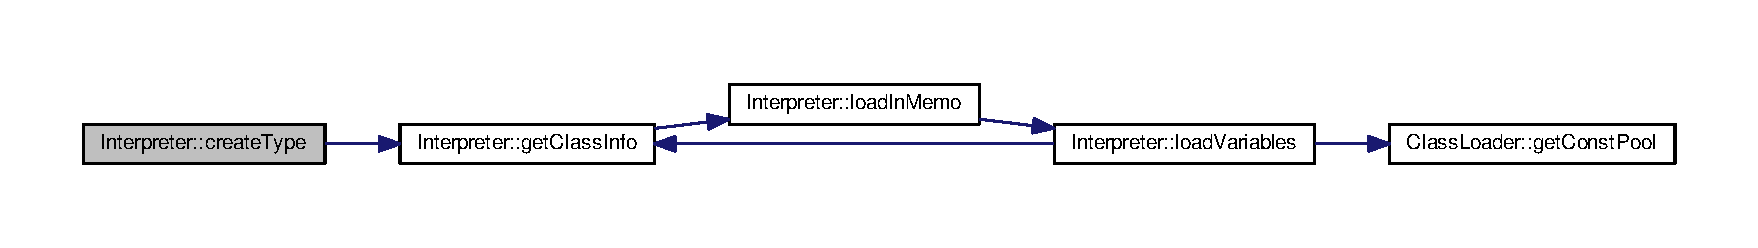
\includegraphics[width=350pt]{class_interpreter_a8ff3509dcc0f48200724b8ae04467495_cgraph}
\end{center}
\end{figure}




Este é o diagrama das funções que utilizam esta função\+:
\nopagebreak
\begin{figure}[H]
\begin{center}
\leavevmode
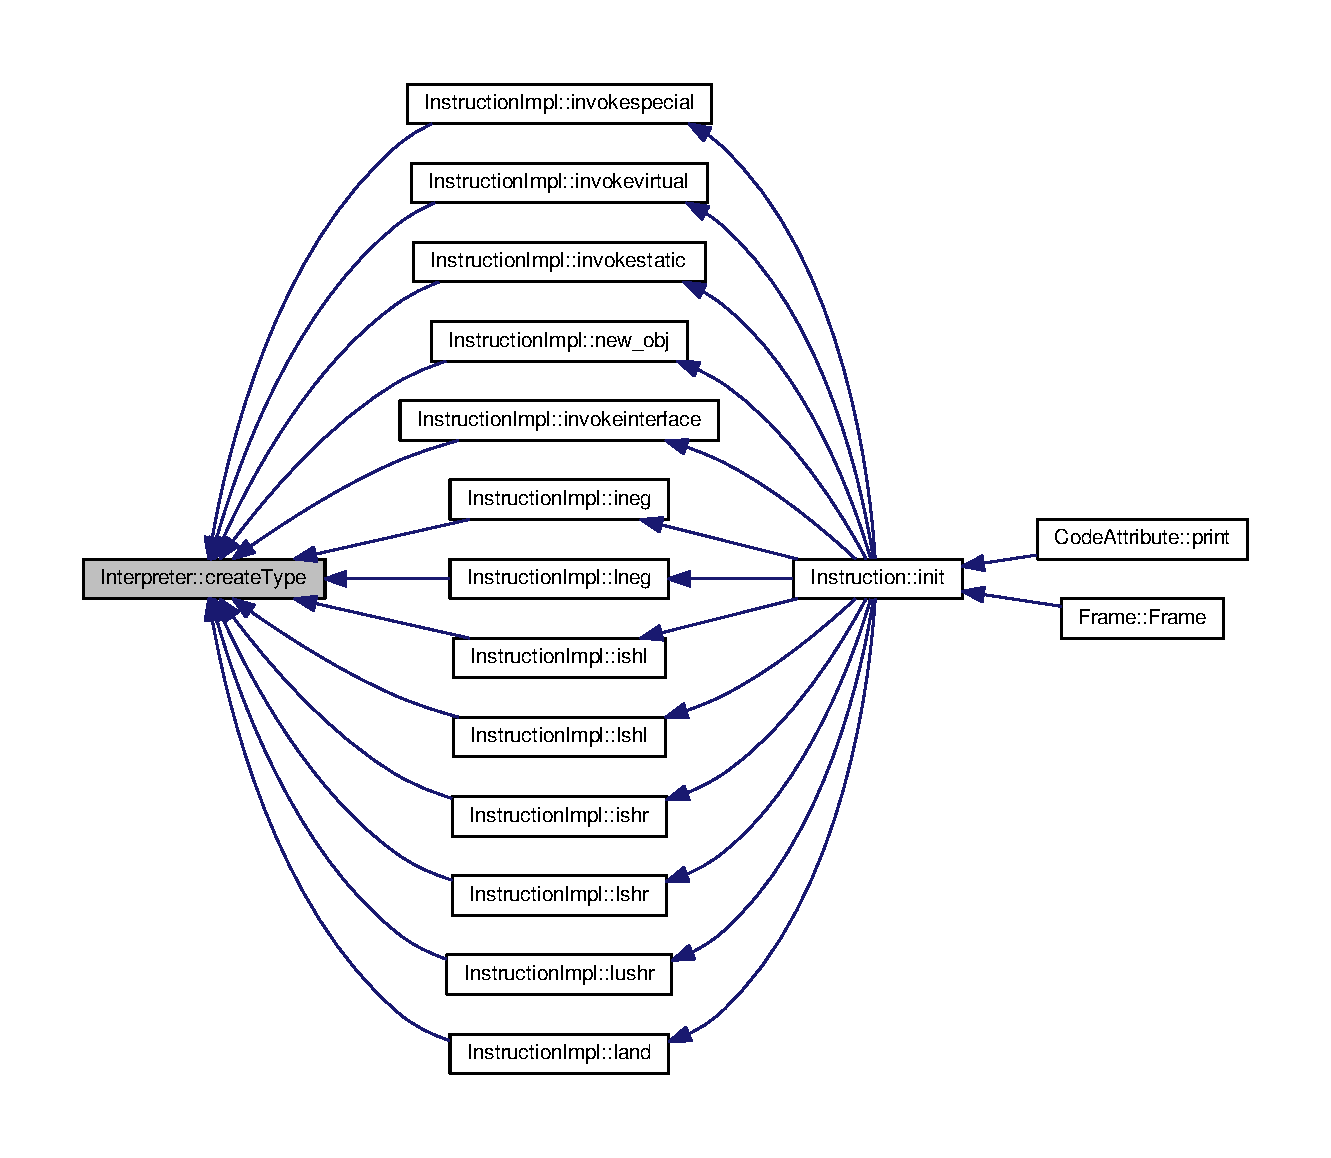
\includegraphics[width=350pt]{class_interpreter_a8ff3509dcc0f48200724b8ae04467495_icgraph}
\end{center}
\end{figure}


\index{Interpreter@{Interpreter}!execute@{execute}}
\index{execute@{execute}!Interpreter@{Interpreter}}
\subsubsection[{\texorpdfstring{execute(\+Class\+Loader $\ast$)}{execute(ClassLoader *)}}]{\setlength{\rightskip}{0pt plus 5cm}void {\bf Interpreter\+::execute} (
\begin{DoxyParamCaption}
\item[{{\bf Class\+Loader} $\ast$}]{classloader}
\end{DoxyParamCaption}
)}\hypertarget{class_interpreter_aaa34fcc8ece810597cd2fea359b65220}{}\label{class_interpreter_aaa34fcc8ece810597cd2fea359b65220}


Grafo de chamadas desta função\+:
\nopagebreak
\begin{figure}[H]
\begin{center}
\leavevmode
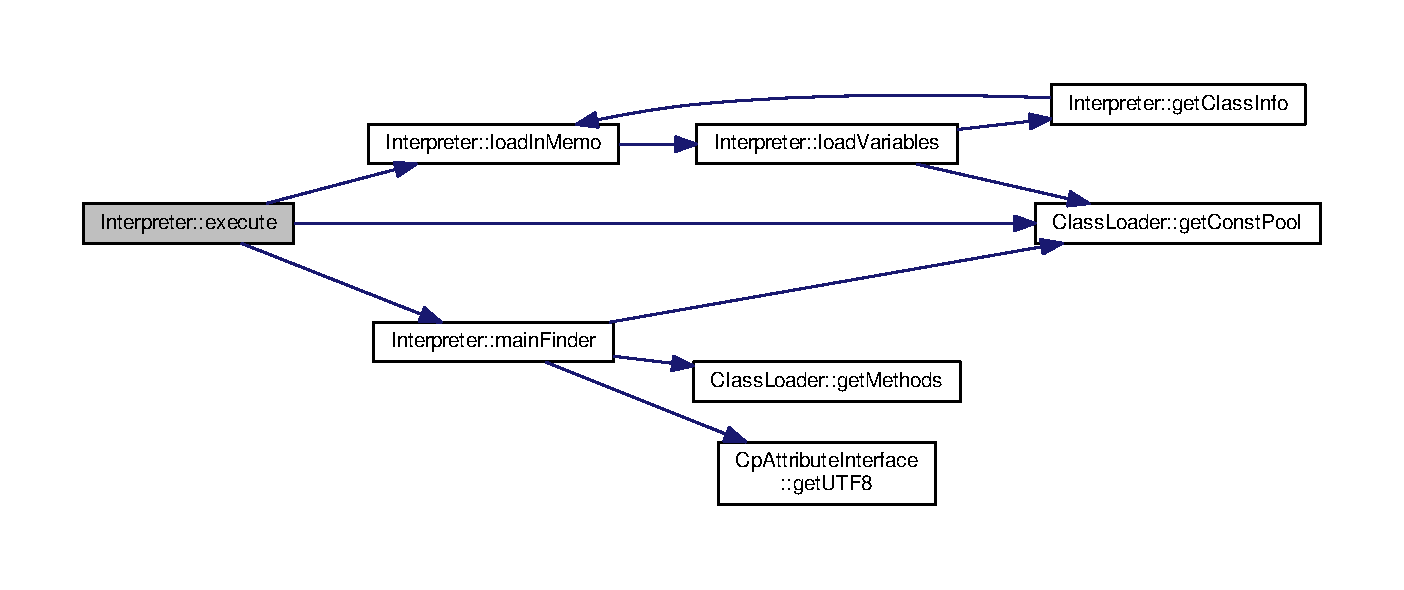
\includegraphics[width=350pt]{class_interpreter_aaa34fcc8ece810597cd2fea359b65220_cgraph}
\end{center}
\end{figure}




Este é o diagrama das funções que utilizam esta função\+:
\nopagebreak
\begin{figure}[H]
\begin{center}
\leavevmode
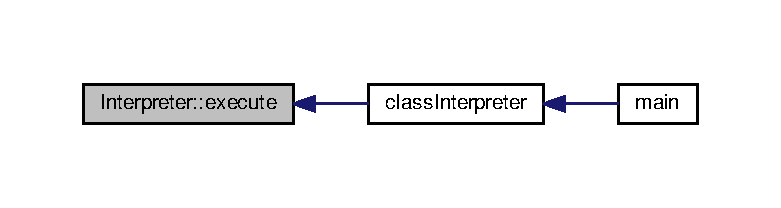
\includegraphics[width=350pt]{class_interpreter_aaa34fcc8ece810597cd2fea359b65220_icgraph}
\end{center}
\end{figure}


\index{Interpreter@{Interpreter}!find\+Method\+By\+Name\+Or\+Descriptor@{find\+Method\+By\+Name\+Or\+Descriptor}}
\index{find\+Method\+By\+Name\+Or\+Descriptor@{find\+Method\+By\+Name\+Or\+Descriptor}!Interpreter@{Interpreter}}
\subsubsection[{\texorpdfstring{find\+Method\+By\+Name\+Or\+Descriptor(\+Class\+Loader $\ast$, std\+::string, std\+::string)}{findMethodByNameOrDescriptor(ClassLoader *, std::string, std::string)}}]{\setlength{\rightskip}{0pt plus 5cm}{\bf Method\+Info} $\ast$ Interpreter\+::find\+Method\+By\+Name\+Or\+Descriptor (
\begin{DoxyParamCaption}
\item[{{\bf Class\+Loader} $\ast$}]{classloader, }
\item[{std\+::string}]{method\+\_\+name, }
\item[{std\+::string}]{method\+\_\+desc}
\end{DoxyParamCaption}
)}\hypertarget{class_interpreter_a16752843b70549dac6ed661365e95ae3}{}\label{class_interpreter_a16752843b70549dac6ed661365e95ae3}


Busca um metodo pelo seu descritor ou nome e o retorna. 


\begin{DoxyParams}{Parâmetros}
{\em $\ast$javaclass} & ponteiro para \hyperlink{class_class_loader}{Class\+Loader}. \\
\hline
{\em string} & que representa o nome do metodo. \\
\hline
{\em string} & que representa o descritor do metodo. \\
\hline
\end{DoxyParams}
\begin{DoxyReturn}{Retorna}
Method\+Info$\ast$ 
\end{DoxyReturn}


Grafo de chamadas desta função\+:
\nopagebreak
\begin{figure}[H]
\begin{center}
\leavevmode
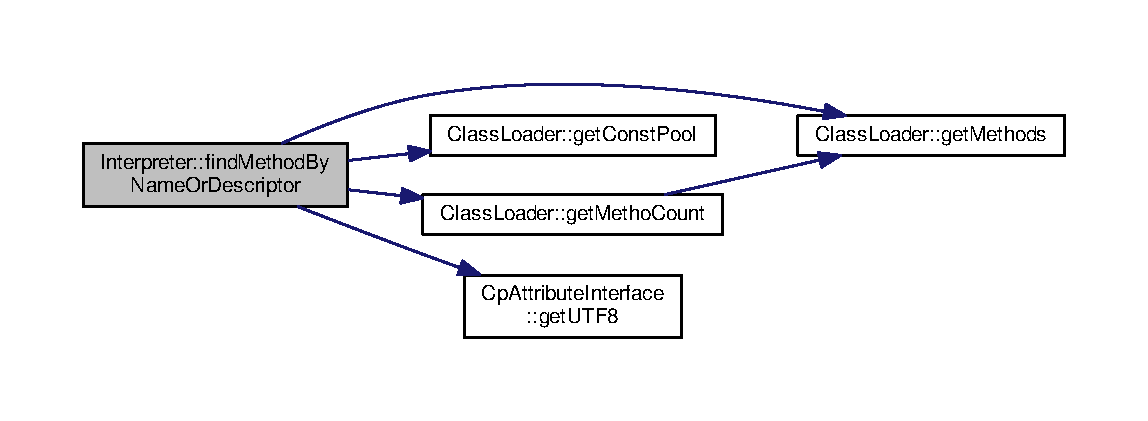
\includegraphics[width=350pt]{class_interpreter_a16752843b70549dac6ed661365e95ae3_cgraph}
\end{center}
\end{figure}




Este é o diagrama das funções que utilizam esta função\+:
\nopagebreak
\begin{figure}[H]
\begin{center}
\leavevmode
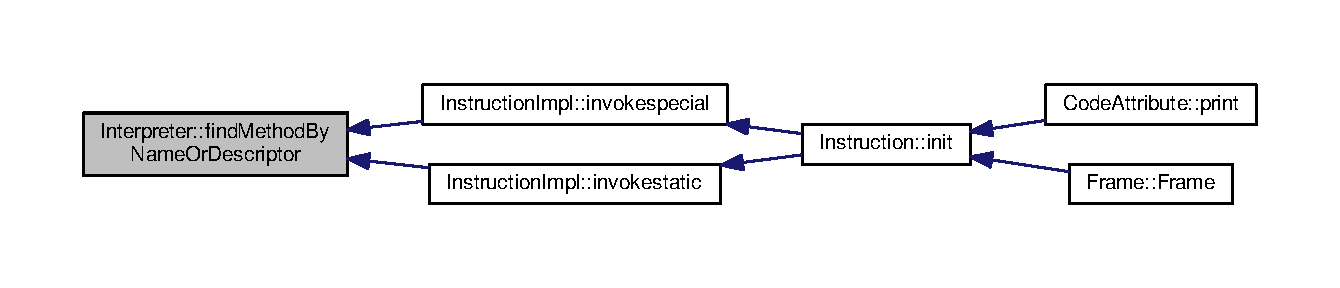
\includegraphics[width=350pt]{class_interpreter_a16752843b70549dac6ed661365e95ae3_icgraph}
\end{center}
\end{figure}


\index{Interpreter@{Interpreter}!get\+Class\+Info@{get\+Class\+Info}}
\index{get\+Class\+Info@{get\+Class\+Info}!Interpreter@{Interpreter}}
\subsubsection[{\texorpdfstring{get\+Class\+Info(std\+::string)}{getClassInfo(std::string)}}]{\setlength{\rightskip}{0pt plus 5cm}{\bf Class\+Loader} $\ast$ {\bf Interpreter\+::get\+Class\+Info} (
\begin{DoxyParamCaption}
\item[{std\+::string}]{class\+Name}
\end{DoxyParamCaption}
)\hspace{0.3cm}{\ttfamily [static]}}\hypertarget{class_interpreter_a99a623bb05c66632d0ab034ebaf2cf51}{}\label{class_interpreter_a99a623bb05c66632d0ab034ebaf2cf51}


Grafo de chamadas desta função\+:
\nopagebreak
\begin{figure}[H]
\begin{center}
\leavevmode
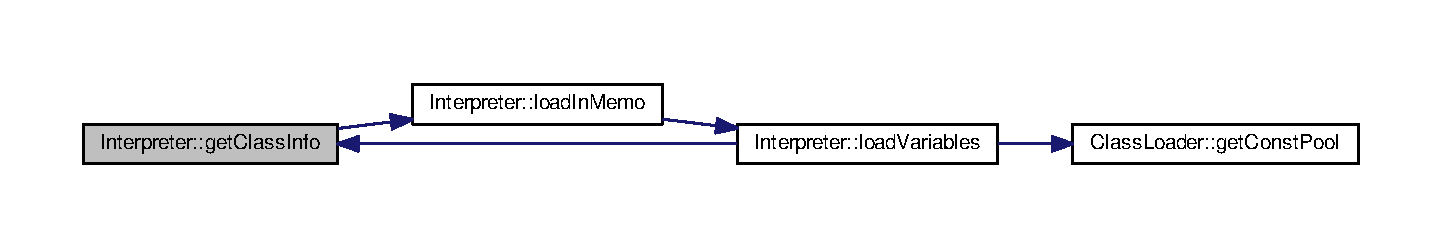
\includegraphics[width=350pt]{class_interpreter_a99a623bb05c66632d0ab034ebaf2cf51_cgraph}
\end{center}
\end{figure}




Este é o diagrama das funções que utilizam esta função\+:
\nopagebreak
\begin{figure}[H]
\begin{center}
\leavevmode
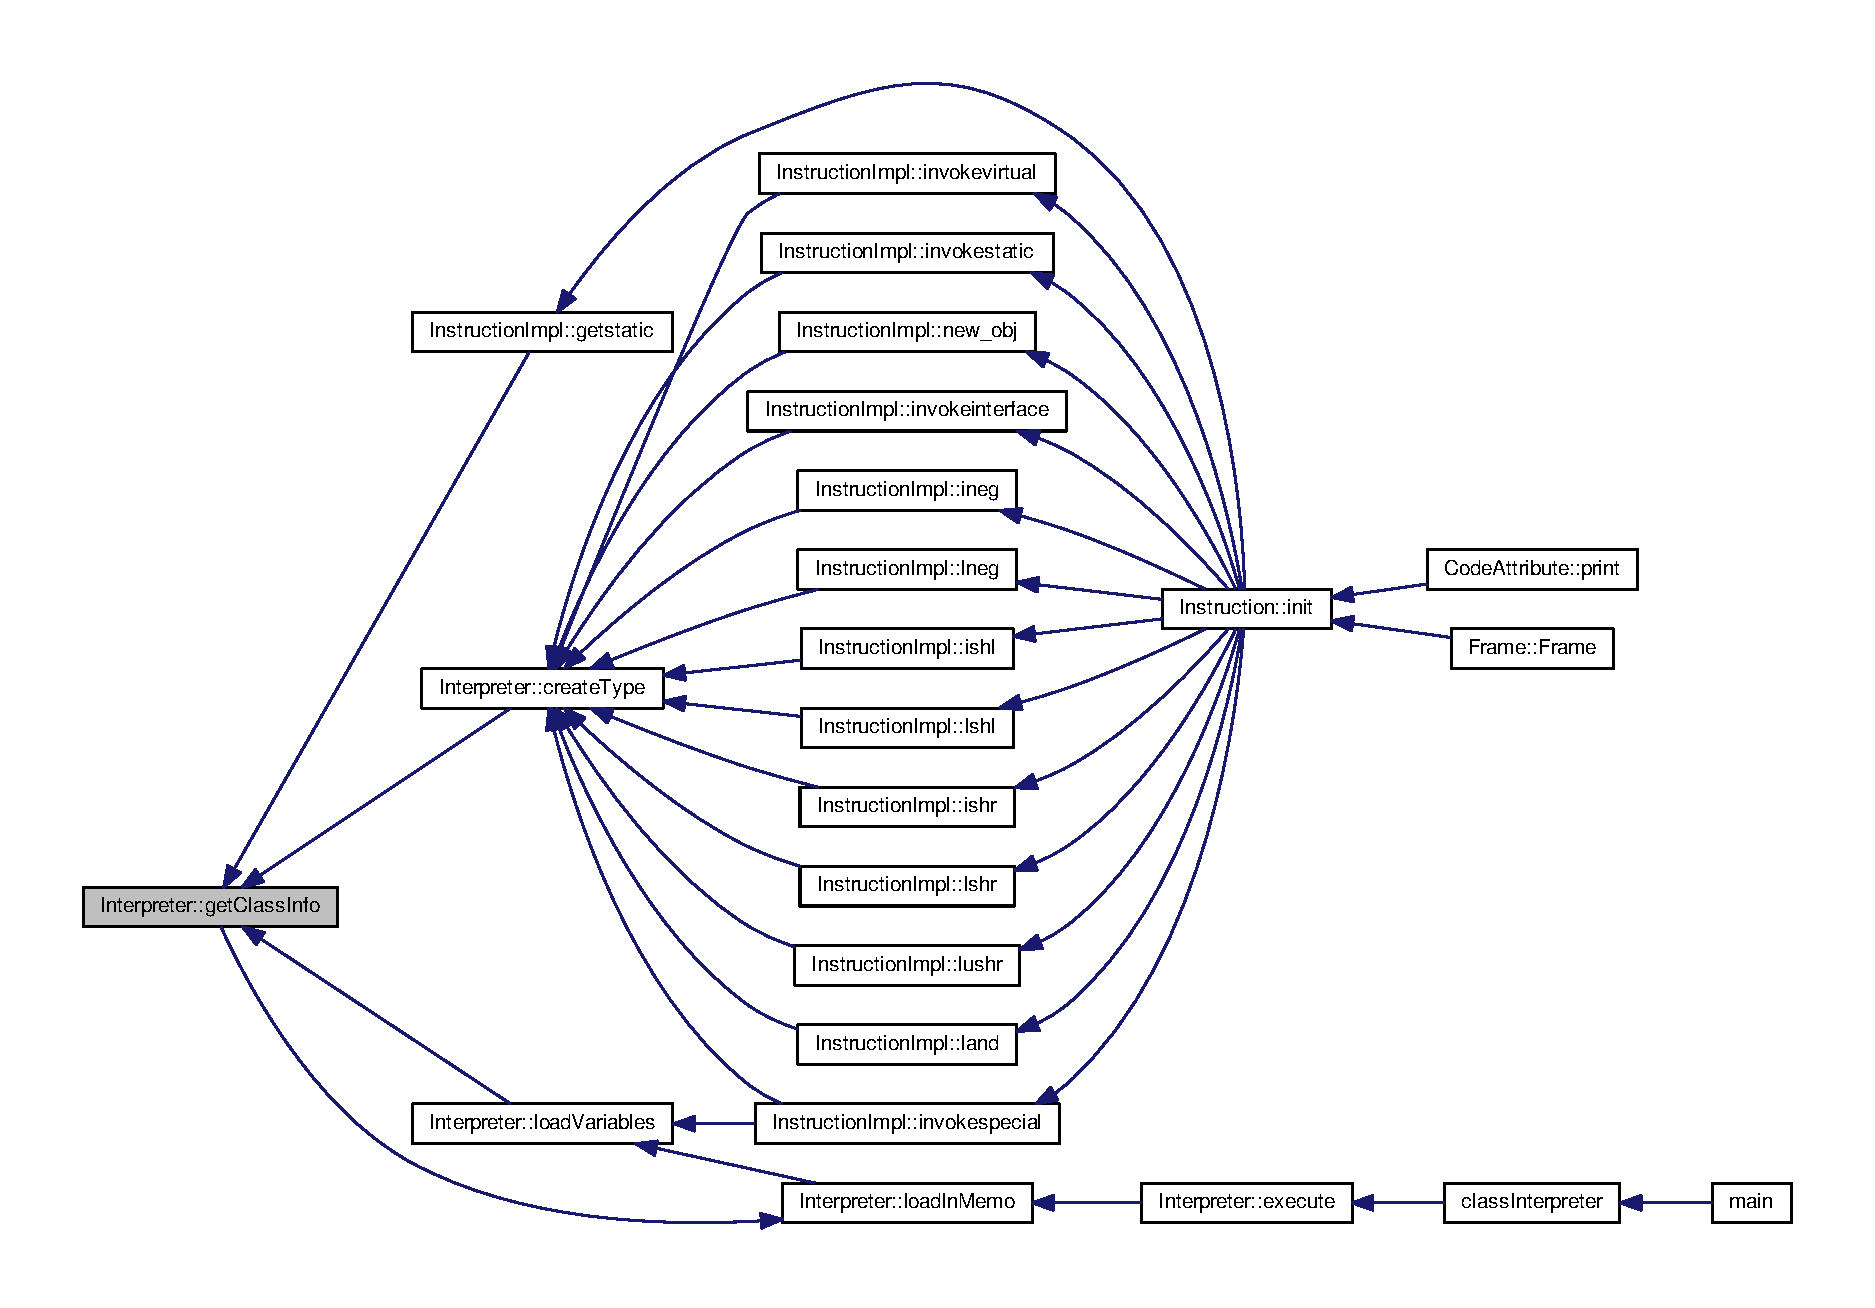
\includegraphics[width=350pt]{class_interpreter_a99a623bb05c66632d0ab034ebaf2cf51_icgraph}
\end{center}
\end{figure}


\index{Interpreter@{Interpreter}!load\+In\+Memo@{load\+In\+Memo}}
\index{load\+In\+Memo@{load\+In\+Memo}!Interpreter@{Interpreter}}
\subsubsection[{\texorpdfstring{load\+In\+Memo(\+Class\+Loader $\ast$)}{loadInMemo(ClassLoader *)}}]{\setlength{\rightskip}{0pt plus 5cm}{\bf Instance} $\ast$ {\bf Interpreter\+::load\+In\+Memo} (
\begin{DoxyParamCaption}
\item[{{\bf Class\+Loader} $\ast$}]{javaclass}
\end{DoxyParamCaption}
)\hspace{0.3cm}{\ttfamily [static]}}\hypertarget{class_interpreter_ab8fa17a7a73d119f3a3113555aef9702}{}\label{class_interpreter_ab8fa17a7a73d119f3a3113555aef9702}


Grafo de chamadas desta função\+:
\nopagebreak
\begin{figure}[H]
\begin{center}
\leavevmode
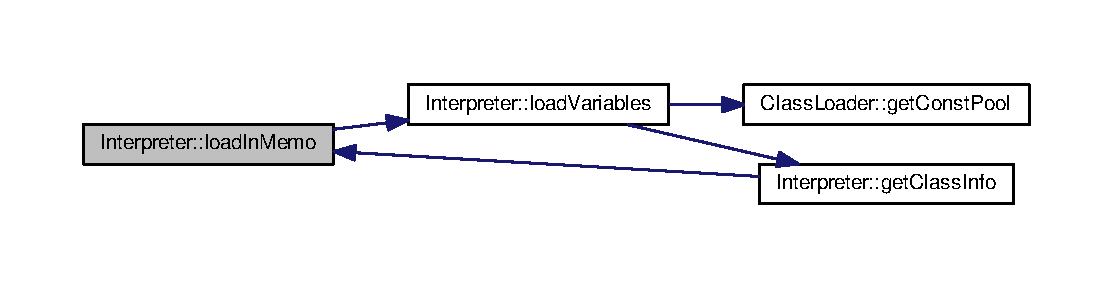
\includegraphics[width=350pt]{class_interpreter_ab8fa17a7a73d119f3a3113555aef9702_cgraph}
\end{center}
\end{figure}




Este é o diagrama das funções que utilizam esta função\+:
\nopagebreak
\begin{figure}[H]
\begin{center}
\leavevmode
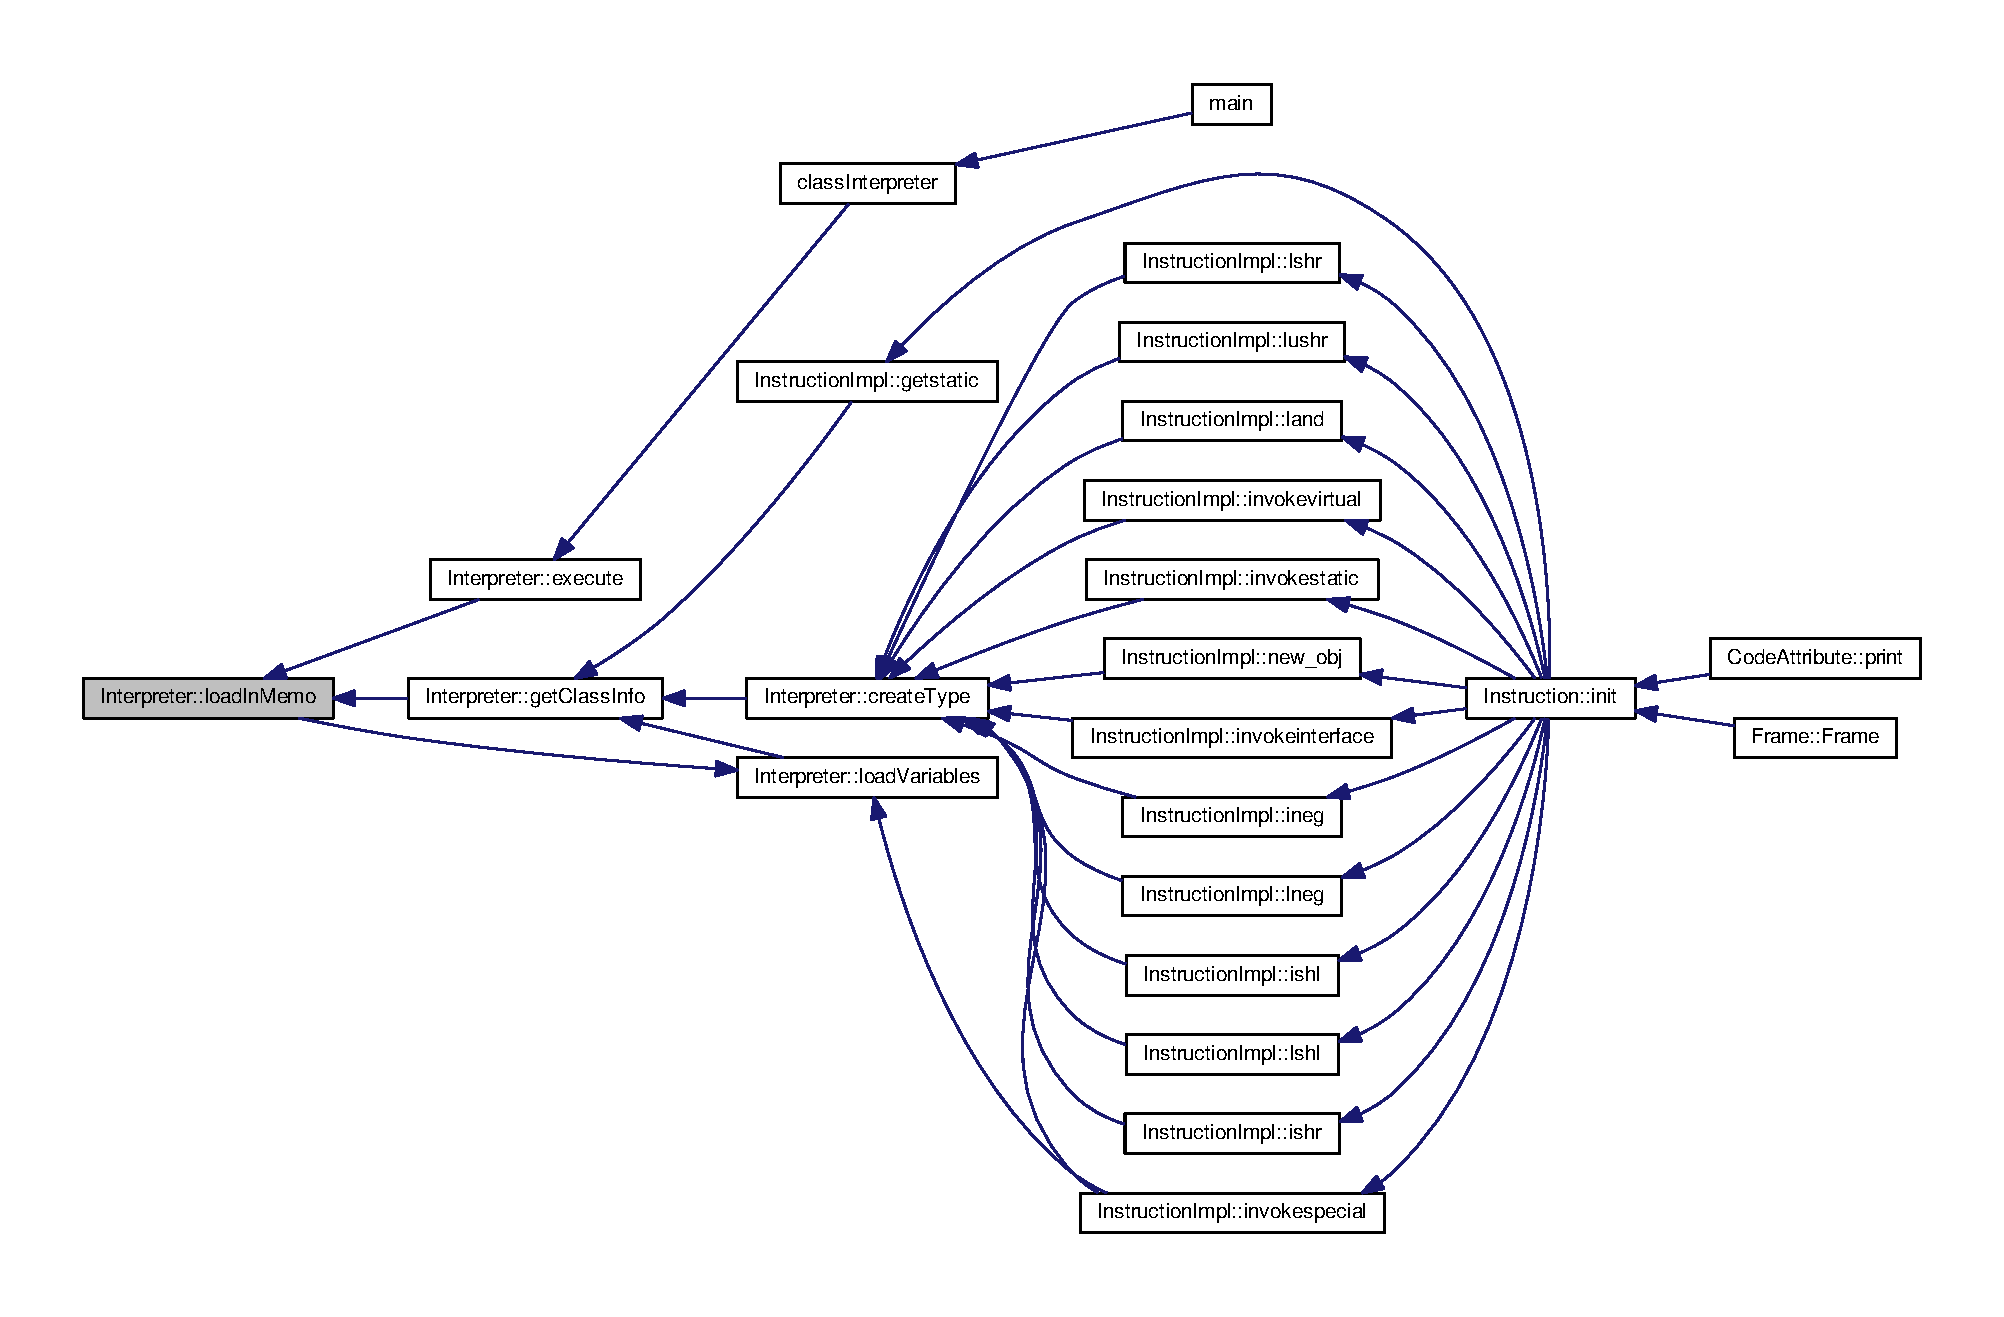
\includegraphics[width=350pt]{class_interpreter_ab8fa17a7a73d119f3a3113555aef9702_icgraph}
\end{center}
\end{figure}


\index{Interpreter@{Interpreter}!load\+Variables@{load\+Variables}}
\index{load\+Variables@{load\+Variables}!Interpreter@{Interpreter}}
\subsubsection[{\texorpdfstring{load\+Variables(\+Instance $\ast$)}{loadVariables(Instance *)}}]{\setlength{\rightskip}{0pt plus 5cm}void {\bf Interpreter\+::load\+Variables} (
\begin{DoxyParamCaption}
\item[{{\bf Instance} $\ast$}]{instance}
\end{DoxyParamCaption}
)\hspace{0.3cm}{\ttfamily [static]}}\hypertarget{class_interpreter_a39a3745e54aa3cee8882075c96ae8b3f}{}\label{class_interpreter_a39a3745e54aa3cee8882075c96ae8b3f}


Grafo de chamadas desta função\+:
\nopagebreak
\begin{figure}[H]
\begin{center}
\leavevmode
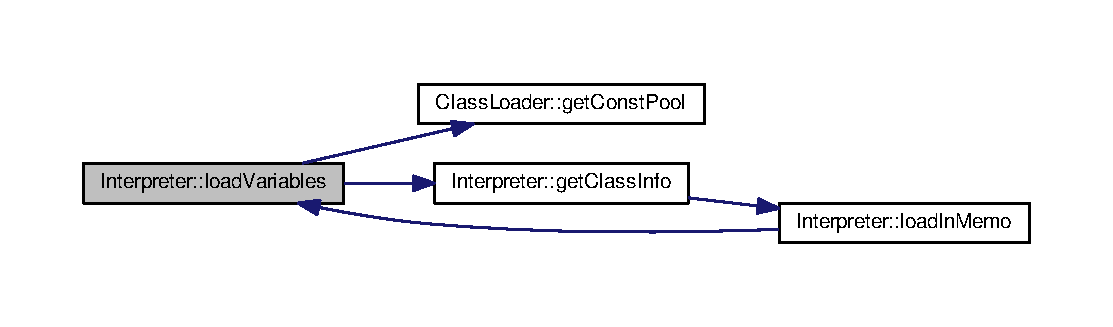
\includegraphics[width=350pt]{class_interpreter_a39a3745e54aa3cee8882075c96ae8b3f_cgraph}
\end{center}
\end{figure}




Este é o diagrama das funções que utilizam esta função\+:
\nopagebreak
\begin{figure}[H]
\begin{center}
\leavevmode
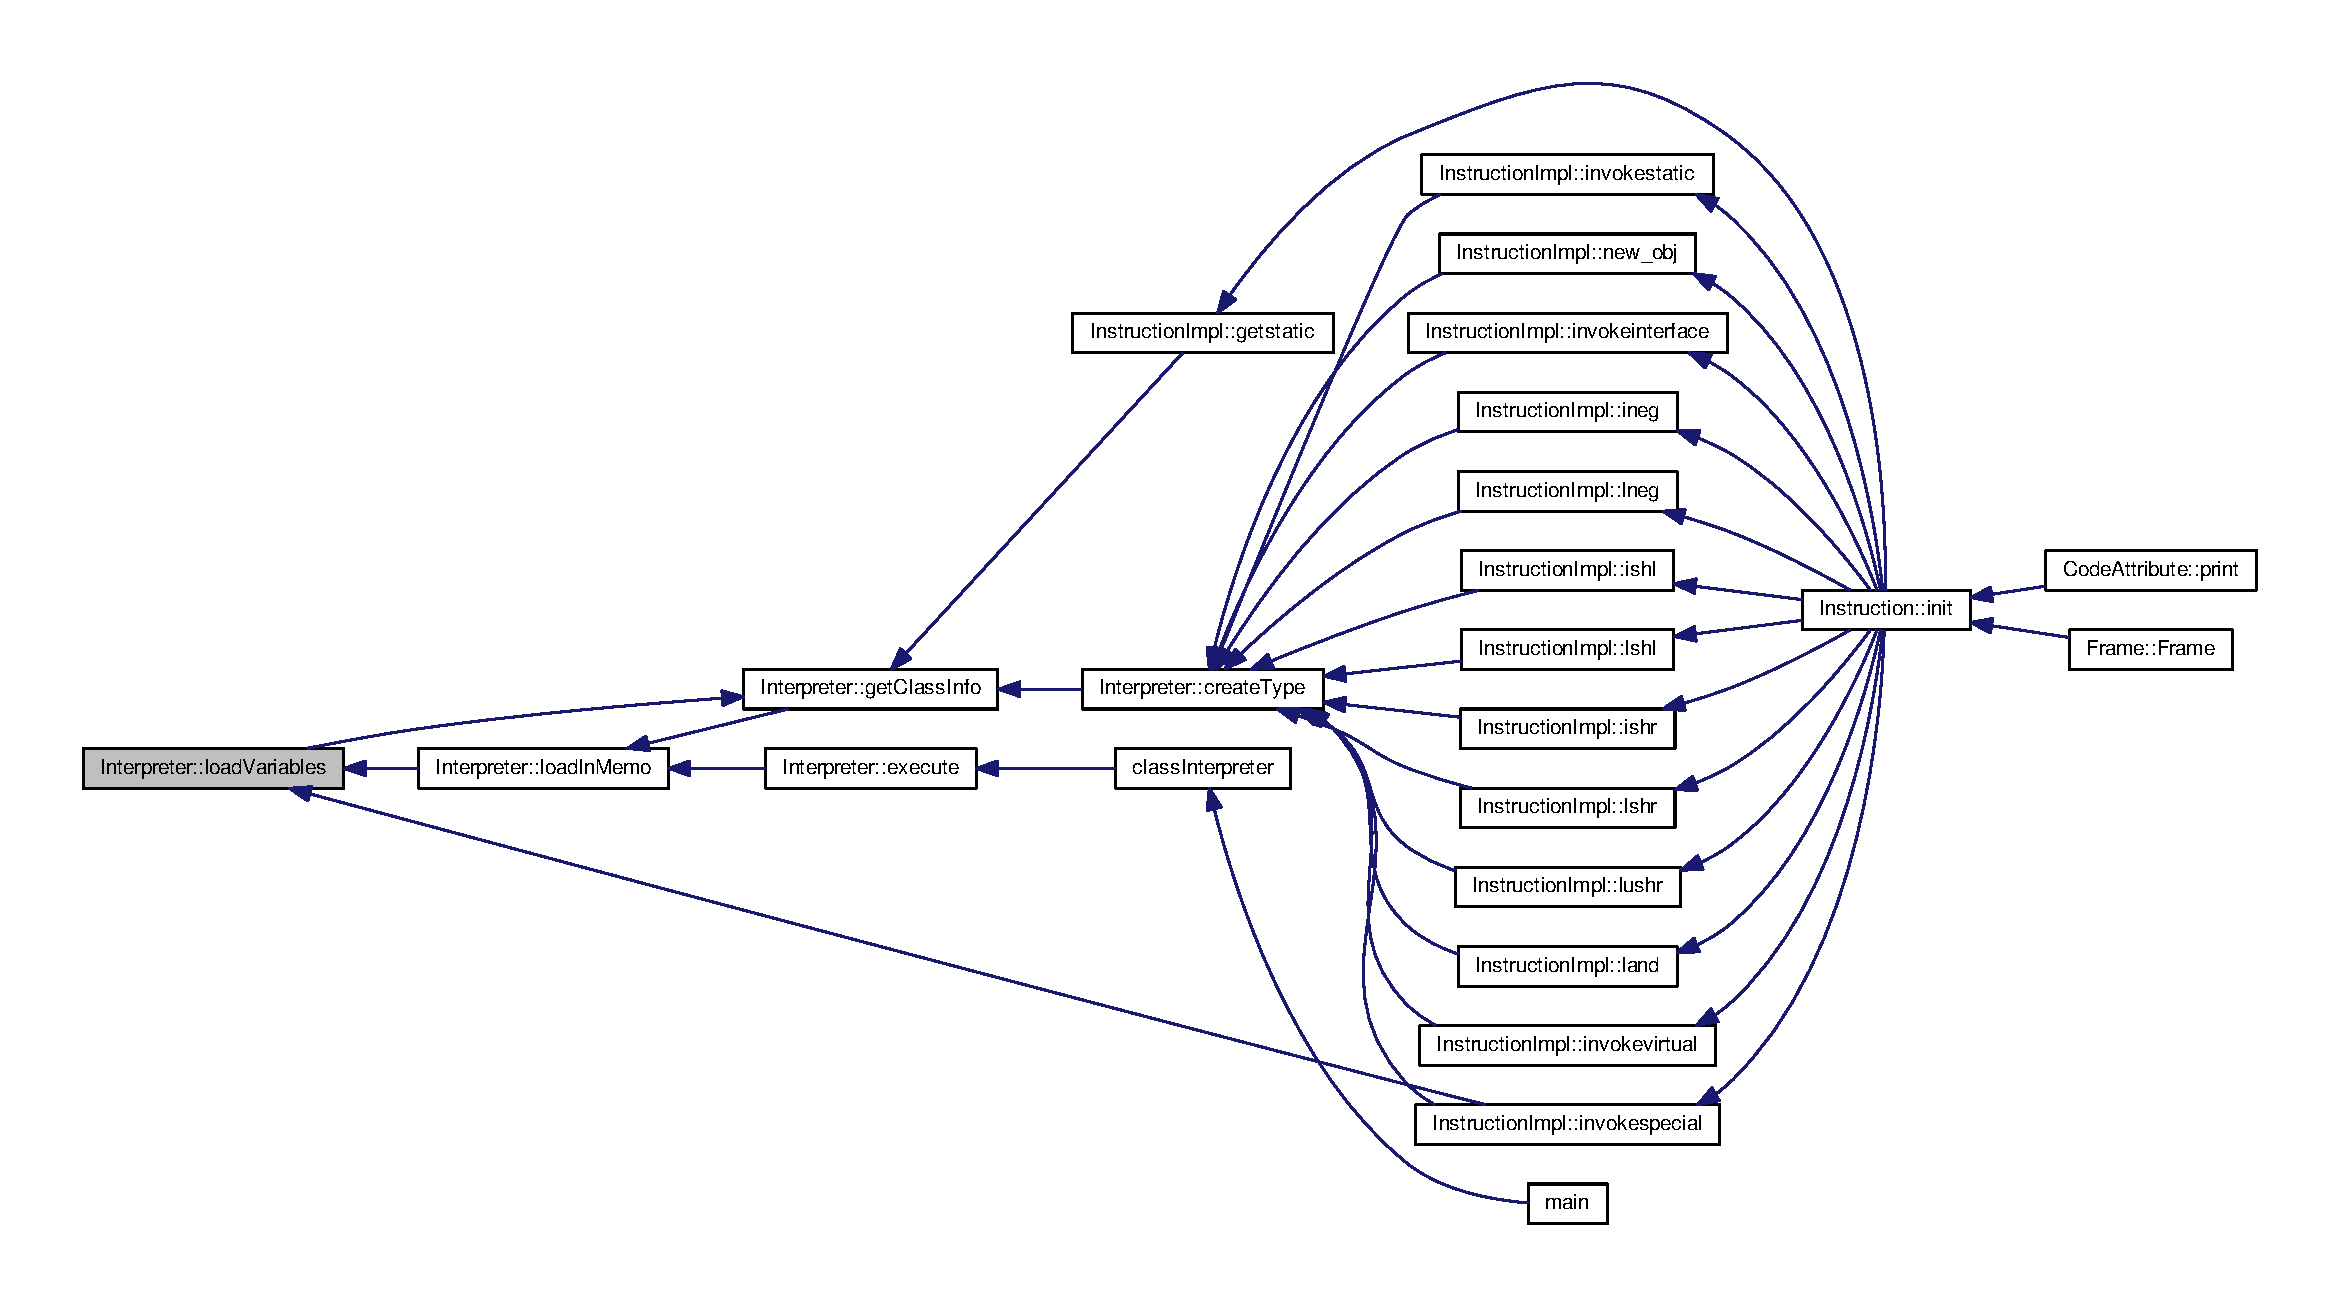
\includegraphics[width=350pt]{class_interpreter_a39a3745e54aa3cee8882075c96ae8b3f_icgraph}
\end{center}
\end{figure}


\index{Interpreter@{Interpreter}!main\+Finder@{main\+Finder}}
\index{main\+Finder@{main\+Finder}!Interpreter@{Interpreter}}
\subsubsection[{\texorpdfstring{main\+Finder(\+Class\+Loader $\ast$)}{mainFinder(ClassLoader *)}}]{\setlength{\rightskip}{0pt plus 5cm}{\bf Method\+Info} $\ast$ {\bf Interpreter\+::main\+Finder} (
\begin{DoxyParamCaption}
\item[{{\bf Class\+Loader} $\ast$}]{javaclass}
\end{DoxyParamCaption}
)}\hypertarget{class_interpreter_a9be1f0faf7df7c81dc180da22ea08fa5}{}\label{class_interpreter_a9be1f0faf7df7c81dc180da22ea08fa5}


Grafo de chamadas desta função\+:
\nopagebreak
\begin{figure}[H]
\begin{center}
\leavevmode
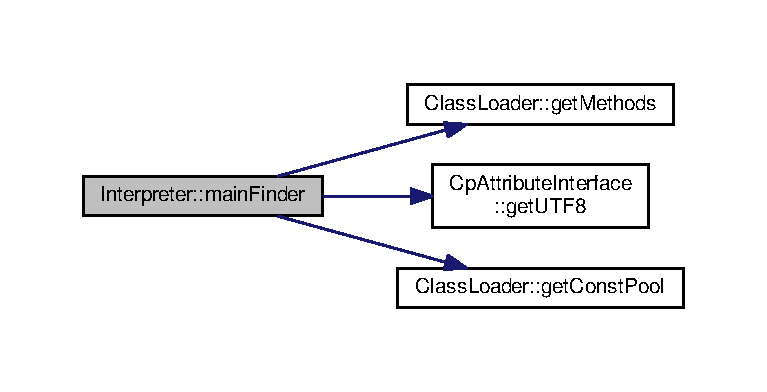
\includegraphics[width=350pt]{class_interpreter_a9be1f0faf7df7c81dc180da22ea08fa5_cgraph}
\end{center}
\end{figure}




Este é o diagrama das funções que utilizam esta função\+:
\nopagebreak
\begin{figure}[H]
\begin{center}
\leavevmode
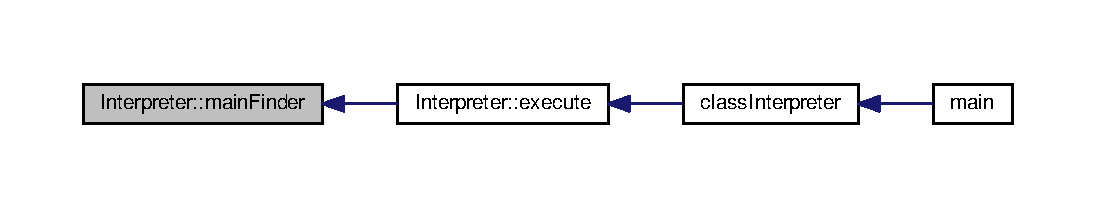
\includegraphics[width=350pt]{class_interpreter_a9be1f0faf7df7c81dc180da22ea08fa5_icgraph}
\end{center}
\end{figure}




\subsection{Documentação dos dados membro}
\index{Interpreter@{Interpreter}!current\+\_\+path\+\_\+folder@{current\+\_\+path\+\_\+folder}}
\index{current\+\_\+path\+\_\+folder@{current\+\_\+path\+\_\+folder}!Interpreter@{Interpreter}}
\subsubsection[{\texorpdfstring{current\+\_\+path\+\_\+folder}{current_path_folder}}]{\setlength{\rightskip}{0pt plus 5cm}std\+::string Interpreter\+::current\+\_\+path\+\_\+folder}\hypertarget{class_interpreter_aba201f836cc30ebda2cdab362e00a145}{}\label{class_interpreter_aba201f836cc30ebda2cdab362e00a145}
\index{Interpreter@{Interpreter}!frame\+\_\+stack@{frame\+\_\+stack}}
\index{frame\+\_\+stack@{frame\+\_\+stack}!Interpreter@{Interpreter}}
\subsubsection[{\texorpdfstring{frame\+\_\+stack}{frame_stack}}]{\setlength{\rightskip}{0pt plus 5cm}std\+::stack$<$ {\bf Frame} $\ast$ $>$ Interpreter\+::frame\+\_\+stack\hspace{0.3cm}{\ttfamily [static]}}\hypertarget{class_interpreter_a58a07f0f8a916fdca9cd97fb220c55dc}{}\label{class_interpreter_a58a07f0f8a916fdca9cd97fb220c55dc}


A documentação para esta classe foi gerada a partir dos seguintes ficheiros\+:\begin{DoxyCompactItemize}
\item 
\hyperlink{_interpreter_8hpp}{Interpreter.\+hpp}\item 
\hyperlink{_interpreter_8cpp}{Interpreter.\+cpp}\end{DoxyCompactItemize}

\hypertarget{class_instruction_impl_1_1invokedynamic}{}\section{Referência à classe Instruction\+Impl\+:\+:invokedynamic}
\label{class_instruction_impl_1_1invokedynamic}\index{Instruction\+Impl\+::invokedynamic@{Instruction\+Impl\+::invokedynamic}}


Invoka o um metodo dinamico.  




\subsection{Descrição detalhada}
Invoka o um metodo dinamico. 


\begin{DoxyParams}{Parâmetros}
{\em $\ast$this\+\_\+frame} & ponteiro para o frame atual \\
\hline
\end{DoxyParams}
\begin{DoxyReturn}{Retorna}
void 
\end{DoxyReturn}


A documentação para esta classe foi gerada a partir do seguinte ficheiro\+:\begin{DoxyCompactItemize}
\item 
\hyperlink{_instruction_impl_8cpp}{Instruction\+Impl.\+cpp}\end{DoxyCompactItemize}

\hypertarget{class_instruction_impl_1_1invokeinterface}{}\section{Referência à classe Instruction\+Impl\+:\+:invokeinterface}
\label{class_instruction_impl_1_1invokeinterface}\index{Instruction\+Impl\+::invokeinterface@{Instruction\+Impl\+::invokeinterface}}


Invoca um metodo declarado com a interface do java.  




\subsection{Descrição detalhada}
Invoca um metodo declarado com a interface do java. 


\begin{DoxyParams}{Parâmetros}
{\em $\ast$this\+\_\+frame} & ponteiro para o frame atual \\
\hline
\end{DoxyParams}
\begin{DoxyReturn}{Retorna}
void 
\end{DoxyReturn}


A documentação para esta classe foi gerada a partir do seguinte ficheiro\+:\begin{DoxyCompactItemize}
\item 
\hyperlink{_instruction_impl_8cpp}{Instruction\+Impl.\+cpp}\end{DoxyCompactItemize}

\hypertarget{class_instruction_impl_1_1invokespecial}{}\section{Referência à classe Instruction\+Impl\+:\+:invokespecial}
\label{class_instruction_impl_1_1invokespecial}\index{Instruction\+Impl\+::invokespecial@{Instruction\+Impl\+::invokespecial}}


Invoca um metodo de instancia.  




\subsection{Descrição detalhada}
Invoca um metodo de instancia. 


\begin{DoxyParams}{Parâmetros}
{\em $\ast$this\+\_\+frame} & ponteiro para o frame atual \\
\hline
\end{DoxyParams}
\begin{DoxyReturn}{Retorna}
void 
\end{DoxyReturn}


A documentação para esta classe foi gerada a partir do seguinte ficheiro\+:\begin{DoxyCompactItemize}
\item 
\hyperlink{_instruction_impl_8cpp}{Instruction\+Impl.\+cpp}\end{DoxyCompactItemize}

\hypertarget{class_instruction_impl_1_1invokestatic}{}\section{Instruction\+Impl\+:\+:invokestatic Class Reference}
\label{class_instruction_impl_1_1invokestatic}\index{Instruction\+Impl\+::invokestatic@{Instruction\+Impl\+::invokestatic}}


Invoca um método de classe.  




\subsection{Detailed Description}
Invoca um método de classe. 


\begin{DoxyParams}{Parameters}
{\em $\ast$this\+\_\+frame} & ponteiro para o frame atual \\
\hline
\end{DoxyParams}
\begin{DoxyReturn}{Returns}
void 
\end{DoxyReturn}


The documentation for this class was generated from the following file\+:\begin{DoxyCompactItemize}
\item 
\hyperlink{_instruction_impl_8cpp}{Instruction\+Impl.\+cpp}\end{DoxyCompactItemize}

\hypertarget{class_instruction_impl_1_1invokevirtual}{}\section{Instruction\+Impl\+:\+:invokevirtual Class Reference}
\label{class_instruction_impl_1_1invokevirtual}\index{Instruction\+Impl\+::invokevirtual@{Instruction\+Impl\+::invokevirtual}}


Invoke instancia um metodo.  




\subsection{Detailed Description}
Invoke instancia um metodo. 


\begin{DoxyParams}{Parameters}
{\em $\ast$this\+\_\+frame} & ponteiro para o frame atual \\
\hline
\end{DoxyParams}
\begin{DoxyReturn}{Returns}
void 
\end{DoxyReturn}


The documentation for this class was generated from the following file\+:\begin{DoxyCompactItemize}
\item 
\hyperlink{_instruction_impl_8cpp}{Instruction\+Impl.\+cpp}\end{DoxyCompactItemize}

\hypertarget{class_instruction_impl_1_1ior}{}\section{Referência à classe Instruction\+Impl\+:\+:ior}
\label{class_instruction_impl_1_1ior}\index{Instruction\+Impl\+::ior@{Instruction\+Impl\+::ior}}


Realiza a operacao de OR entre dois operandos e empilha o resultado.  




\subsection{Descrição detalhada}
Realiza a operacao de OR entre dois operandos e empilha o resultado. 


\begin{DoxyParams}{Parâmetros}
{\em $\ast$this\+\_\+frame} & ponteiro para o frame atual \\
\hline
\end{DoxyParams}
\begin{DoxyReturn}{Retorna}
void 
\end{DoxyReturn}


A documentação para esta classe foi gerada a partir do seguinte ficheiro\+:\begin{DoxyCompactItemize}
\item 
\hyperlink{_instruction_impl_8cpp}{Instruction\+Impl.\+cpp}\end{DoxyCompactItemize}

\hypertarget{class_instruction_impl_1_1irem}{}\section{Instruction\+Impl\+:\+:irem Class Reference}
\label{class_instruction_impl_1_1irem}\index{Instruction\+Impl\+::irem@{Instruction\+Impl\+::irem}}


Resto de inteiro.  




\subsection{Detailed Description}
Resto de inteiro. 


\begin{DoxyParams}{Parameters}
{\em $\ast$this\+\_\+frame} & Ponteiro para o frame atual \\
\hline
\end{DoxyParams}
\begin{DoxyReturn}{Returns}
void 
\end{DoxyReturn}


The documentation for this class was generated from the following file\+:\begin{DoxyCompactItemize}
\item 
\hyperlink{_instruction_impl_8cpp}{Instruction\+Impl.\+cpp}\end{DoxyCompactItemize}

\hypertarget{class_instruction_impl_1_1ireturn}{}\section{Referência à classe Instruction\+Impl\+:\+:ireturn}
\label{class_instruction_impl_1_1ireturn}\index{Instruction\+Impl\+::ireturn@{Instruction\+Impl\+::ireturn}}


Retorna int de um método.  




\subsection{Descrição detalhada}
Retorna int de um método. 


\begin{DoxyParams}{Parâmetros}
{\em $\ast$this\+\_\+frame} & ponteiro para o frame atual \\
\hline
\end{DoxyParams}
\begin{DoxyReturn}{Retorna}
void 
\end{DoxyReturn}


A documentação para esta classe foi gerada a partir do seguinte ficheiro\+:\begin{DoxyCompactItemize}
\item 
\hyperlink{_instruction_impl_8cpp}{Instruction\+Impl.\+cpp}\end{DoxyCompactItemize}

\hypertarget{class_instruction_impl_1_1ishl}{}\section{Instruction\+Impl\+:\+:ishl Class Reference}
\label{class_instruction_impl_1_1ishl}\index{Instruction\+Impl\+::ishl@{Instruction\+Impl\+::ishl}}


Calcula o valor do shift left lógico para inteiro. Retira dois operandos do topo da pilha e faz o shift left do primeiro operando por s posições, onde s são os 5 bits menos significativos do segundo operando. O resultado é colocado no topo da pilha.  




\subsection{Detailed Description}
Calcula o valor do shift left lógico para inteiro. Retira dois operandos do topo da pilha e faz o shift left do primeiro operando por s posições, onde s são os 5 bits menos significativos do segundo operando. O resultado é colocado no topo da pilha. 


\begin{DoxyParams}{Parameters}
{\em $\ast$this\+\_\+frame} & Ponteiro para o frame atual \\
\hline
\end{DoxyParams}
\begin{DoxyReturn}{Returns}
void 
\end{DoxyReturn}


The documentation for this class was generated from the following file\+:\begin{DoxyCompactItemize}
\item 
\hyperlink{_instruction_impl_8cpp}{Instruction\+Impl.\+cpp}\end{DoxyCompactItemize}

\hypertarget{class_instruction_impl_1_1ishr}{}\section{Referência à classe Instruction\+Impl\+:\+:ishr}
\label{class_instruction_impl_1_1ishr}\index{Instruction\+Impl\+::ishr@{Instruction\+Impl\+::ishr}}


Calcula o valor do shift right lógico para inteiro. Retira dois operandos do topo da pilha e faz o shift right do primeiro operando por s posições, onde s são os 5 bits menos significativos do segundo operando. O resultado é colocado no topo da pilha.  




\subsection{Descrição detalhada}
Calcula o valor do shift right lógico para inteiro. Retira dois operandos do topo da pilha e faz o shift right do primeiro operando por s posições, onde s são os 5 bits menos significativos do segundo operando. O resultado é colocado no topo da pilha. 


\begin{DoxyParams}{Parâmetros}
{\em $\ast$this\+\_\+frame} & Ponteiro para o frame atual \\
\hline
\end{DoxyParams}
\begin{DoxyReturn}{Retorna}
void 
\end{DoxyReturn}


A documentação para esta classe foi gerada a partir do seguinte ficheiro\+:\begin{DoxyCompactItemize}
\item 
\hyperlink{_instruction_impl_8cpp}{Instruction\+Impl.\+cpp}\end{DoxyCompactItemize}

\hypertarget{class_instruction_impl_1_1istore}{}\section{Instruction\+Impl\+:\+:istore Class Reference}
\label{class_instruction_impl_1_1istore}\index{Instruction\+Impl\+::istore@{Instruction\+Impl\+::istore}}


Armazena um inteiro no array de variaveis locais no valor indicado pelo indice.  




\subsection{Detailed Description}
Armazena um inteiro no array de variaveis locais no valor indicado pelo indice. 


\begin{DoxyParams}{Parameters}
{\em $\ast$this\+\_\+frame} & Ponteiro para o frame atual \\
\hline
\end{DoxyParams}
\begin{DoxyReturn}{Returns}
void 
\end{DoxyReturn}


The documentation for this class was generated from the following file\+:\begin{DoxyCompactItemize}
\item 
\hyperlink{_instruction_impl_8cpp}{Instruction\+Impl.\+cpp}\end{DoxyCompactItemize}

\hypertarget{class_instruction_impl_1_1istore__0}{}\section{Instruction\+Impl\+:\+:istore\+\_\+0 Class Reference}
\label{class_instruction_impl_1_1istore__0}\index{Instruction\+Impl\+::istore\+\_\+0@{Instruction\+Impl\+::istore\+\_\+0}}


Armazena um inteiro no array de variaveis locais no indice 0.  




\subsection{Detailed Description}
Armazena um inteiro no array de variaveis locais no indice 0. 


\begin{DoxyParams}{Parameters}
{\em $\ast$this\+\_\+frame} & Ponteiro para o frame atual \\
\hline
\end{DoxyParams}
\begin{DoxyReturn}{Returns}
void 
\end{DoxyReturn}


The documentation for this class was generated from the following file\+:\begin{DoxyCompactItemize}
\item 
\hyperlink{_instruction_impl_8cpp}{Instruction\+Impl.\+cpp}\end{DoxyCompactItemize}

\hypertarget{class_instruction_impl_1_1istore__1}{}\section{Instruction\+Impl\+:\+:istore\+\_\+1 Class Reference}
\label{class_instruction_impl_1_1istore__1}\index{Instruction\+Impl\+::istore\+\_\+1@{Instruction\+Impl\+::istore\+\_\+1}}


Armazena um inteiro no array de variaveis locais no indice 1.  




\subsection{Detailed Description}
Armazena um inteiro no array de variaveis locais no indice 1. 


\begin{DoxyParams}{Parameters}
{\em $\ast$this\+\_\+frame} & Ponteiro para o frame atual \\
\hline
\end{DoxyParams}
\begin{DoxyReturn}{Returns}
void 
\end{DoxyReturn}


The documentation for this class was generated from the following file\+:\begin{DoxyCompactItemize}
\item 
\hyperlink{_instruction_impl_8cpp}{Instruction\+Impl.\+cpp}\end{DoxyCompactItemize}

\hypertarget{class_instruction_impl_1_1istore__2}{}\section{Instruction\+Impl\+:\+:istore\+\_\+2 Class Reference}
\label{class_instruction_impl_1_1istore__2}\index{Instruction\+Impl\+::istore\+\_\+2@{Instruction\+Impl\+::istore\+\_\+2}}


Armazena um inteiro no array de variaveis locais no indice 2.  




\subsection{Detailed Description}
Armazena um inteiro no array de variaveis locais no indice 2. 


\begin{DoxyParams}{Parameters}
{\em $\ast$this\+\_\+frame} & Ponteiro para o frame atual \\
\hline
\end{DoxyParams}
\begin{DoxyReturn}{Returns}
void 
\end{DoxyReturn}


The documentation for this class was generated from the following file\+:\begin{DoxyCompactItemize}
\item 
\hyperlink{_instruction_impl_8cpp}{Instruction\+Impl.\+cpp}\end{DoxyCompactItemize}

\hypertarget{class_instruction_impl_1_1istore__3}{}\section{Instruction\+Impl\+:\+:istore\+\_\+3 Class Reference}
\label{class_instruction_impl_1_1istore__3}\index{Instruction\+Impl\+::istore\+\_\+3@{Instruction\+Impl\+::istore\+\_\+3}}


Armazena um inteiro no array de variaveis locais no indice 3.  




\subsection{Detailed Description}
Armazena um inteiro no array de variaveis locais no indice 3. 


\begin{DoxyParams}{Parameters}
{\em $\ast$this\+\_\+frame} & Ponteiro para o frame atual \\
\hline
\end{DoxyParams}
\begin{DoxyReturn}{Returns}
void 
\end{DoxyReturn}


The documentation for this class was generated from the following file\+:\begin{DoxyCompactItemize}
\item 
\hyperlink{_instruction_impl_8cpp}{Instruction\+Impl.\+cpp}\end{DoxyCompactItemize}

\hypertarget{class_instruction_impl_1_1isub}{}\section{Referência à classe Instruction\+Impl\+:\+:isub}
\label{class_instruction_impl_1_1isub}\index{Instruction\+Impl\+::isub@{Instruction\+Impl\+::isub}}


Desempilha dois inteiros e empilha a subtração dos mesmos.  




\subsection{Descrição detalhada}
Desempilha dois inteiros e empilha a subtração dos mesmos. 


\begin{DoxyParams}{Parâmetros}
{\em $\ast$this\+\_\+frame} & ponteiro para o frame atual \\
\hline
\end{DoxyParams}
\begin{DoxyReturn}{Retorna}
void 
\end{DoxyReturn}


A documentação para esta classe foi gerada a partir do seguinte ficheiro\+:\begin{DoxyCompactItemize}
\item 
\hyperlink{_instruction_impl_8cpp}{Instruction\+Impl.\+cpp}\end{DoxyCompactItemize}

\hypertarget{class_instruction_impl_1_1iushr}{}\section{Referência à classe Instruction\+Impl\+:\+:iushr}
\label{class_instruction_impl_1_1iushr}\index{Instruction\+Impl\+::iushr@{Instruction\+Impl\+::iushr}}


Desempilha dois valores inteiros da pilha, realiza o shift para a direita do número de bits,indicados pelos 2 valor do stack e empilha o resultado.  




\subsection{Descrição detalhada}
Desempilha dois valores inteiros da pilha, realiza o shift para a direita do número de bits,indicados pelos 2 valor do stack e empilha o resultado. 


\begin{DoxyParams}{Parâmetros}
{\em this\+\_\+frame} & Ponteiro para frame corrente. \\
\hline
\end{DoxyParams}
\begin{DoxyReturn}{Retorna}

\end{DoxyReturn}


A documentação para esta classe foi gerada a partir do seguinte ficheiro\+:\begin{DoxyCompactItemize}
\item 
\hyperlink{_instruction_impl_8cpp}{Instruction\+Impl.\+cpp}\end{DoxyCompactItemize}

\hypertarget{class_instruction_impl_1_1ixor}{}\section{Instruction\+Impl\+:\+:ixor Class Reference}
\label{class_instruction_impl_1_1ixor}\index{Instruction\+Impl\+::ixor@{Instruction\+Impl\+::ixor}}


Boolean X\+OR inteiro.  




\subsection{Detailed Description}
Boolean X\+OR inteiro. 


\begin{DoxyParams}{Parameters}
{\em $\ast$this\+\_\+frame} & ponteiro para o frame atual.  \\
\hline
\end{DoxyParams}


The documentation for this class was generated from the following file\+:\begin{DoxyCompactItemize}
\item 
\hyperlink{_instruction_impl_8cpp}{Instruction\+Impl.\+cpp}\end{DoxyCompactItemize}

\hypertarget{class_instruction_impl_1_1jsr}{}\section{Referência à classe Instruction\+Impl\+:\+:jsr}
\label{class_instruction_impl_1_1jsr}\index{Instruction\+Impl\+::jsr@{Instruction\+Impl\+::jsr}}


Instruçao que executa o desvio salvando o endereco de retorno na pilha de operandos.  




\subsection{Descrição detalhada}
Instruçao que executa o desvio salvando o endereco de retorno na pilha de operandos. 


\begin{DoxyParams}{Parâmetros}
{\em $\ast$this\+\_\+frame} & ponteiro para o frame atual \\
\hline
\end{DoxyParams}
\begin{DoxyReturn}{Retorna}
void 
\end{DoxyReturn}


A documentação para esta classe foi gerada a partir do seguinte ficheiro\+:\begin{DoxyCompactItemize}
\item 
\hyperlink{_instruction_impl_8cpp}{Instruction\+Impl.\+cpp}\end{DoxyCompactItemize}

\hypertarget{class_instruction_impl_1_1jsr__w}{}\section{Instruction\+Impl\+:\+:jsr\+\_\+w Class Reference}
\label{class_instruction_impl_1_1jsr__w}\index{Instruction\+Impl\+::jsr\+\_\+w@{Instruction\+Impl\+::jsr\+\_\+w}}


Instruçao que executa o desvio salvando o endereco de retorno na pilha de operandos.  




\subsection{Detailed Description}
Instruçao que executa o desvio salvando o endereco de retorno na pilha de operandos. 


\begin{DoxyParams}{Parameters}
{\em $\ast$this\+\_\+frame} & ponteiro para o frame atual \\
\hline
\end{DoxyParams}
\begin{DoxyReturn}{Returns}
void 
\end{DoxyReturn}


The documentation for this class was generated from the following file\+:\begin{DoxyCompactItemize}
\item 
\hyperlink{_instruction_impl_8cpp}{Instruction\+Impl.\+cpp}\end{DoxyCompactItemize}

\hypertarget{class_instruction_impl_1_1l2d}{}\section{Referência à classe Instruction\+Impl\+:\+:l2d}
\label{class_instruction_impl_1_1l2d}\index{Instruction\+Impl\+::l2d@{Instruction\+Impl\+::l2d}}


Função que desempilha um long, converte para um float e empilha novamente.  




\subsection{Descrição detalhada}
Função que desempilha um long, converte para um float e empilha novamente. 


\begin{DoxyParams}{Parâmetros}
{\em this\+\_\+frame} & Ponteiro para frame. \\
\hline
\end{DoxyParams}
\begin{DoxyReturn}{Retorna}
void 
\end{DoxyReturn}


A documentação para esta classe foi gerada a partir do seguinte ficheiro\+:\begin{DoxyCompactItemize}
\item 
\hyperlink{_instruction_impl_8cpp}{Instruction\+Impl.\+cpp}\end{DoxyCompactItemize}

\hypertarget{class_instruction_impl_1_1l2f}{}\section{Referência à classe Instruction\+Impl\+:\+:l2f}
\label{class_instruction_impl_1_1l2f}\index{Instruction\+Impl\+::l2f@{Instruction\+Impl\+::l2f}}


Função que desempilha um long, converte para um float e empilha novamente.  




\subsection{Descrição detalhada}
Função que desempilha um long, converte para um float e empilha novamente. 


\begin{DoxyParams}{Parâmetros}
{\em this\+\_\+frame} & Ponteiro para frame. \\
\hline
\end{DoxyParams}
\begin{DoxyReturn}{Retorna}
void 
\end{DoxyReturn}


A documentação para esta classe foi gerada a partir do seguinte ficheiro\+:\begin{DoxyCompactItemize}
\item 
\hyperlink{_instruction_impl_8cpp}{Instruction\+Impl.\+cpp}\end{DoxyCompactItemize}

\hypertarget{class_instruction_impl_1_1l2i}{}\section{Instruction\+Impl\+:\+:l2i Class Reference}
\label{class_instruction_impl_1_1l2i}\index{Instruction\+Impl\+::l2i@{Instruction\+Impl\+::l2i}}


Função que desempilha um long, converte para inteiro e empilha novamente.  




\subsection{Detailed Description}
Função que desempilha um long, converte para inteiro e empilha novamente. 


\begin{DoxyParams}{Parameters}
{\em frame} & Ponteiro para frame. \\
\hline
\end{DoxyParams}
\begin{DoxyReturn}{Returns}
void 
\end{DoxyReturn}


The documentation for this class was generated from the following file\+:\begin{DoxyCompactItemize}
\item 
\hyperlink{_instruction_impl_8cpp}{Instruction\+Impl.\+cpp}\end{DoxyCompactItemize}

\hypertarget{class_instruction_impl_1_1ladd}{}\section{Instruction\+Impl\+:\+:ladd Class Reference}
\label{class_instruction_impl_1_1ladd}\index{Instruction\+Impl\+::ladd@{Instruction\+Impl\+::ladd}}


Soma do tipo long. Retira os dois operando do topo da pilha, soma-\/os e coloca o resultado no topo da pilha.  




\subsection{Detailed Description}
Soma do tipo long. Retira os dois operando do topo da pilha, soma-\/os e coloca o resultado no topo da pilha. 


\begin{DoxyParams}{Parameters}
{\em $\ast$this\+\_\+frame} & Ponteiro para o frame atual \\
\hline
\end{DoxyParams}
\begin{DoxyReturn}{Returns}
void 
\end{DoxyReturn}


The documentation for this class was generated from the following file\+:\begin{DoxyCompactItemize}
\item 
\hyperlink{_instruction_impl_8cpp}{Instruction\+Impl.\+cpp}\end{DoxyCompactItemize}

\hypertarget{class_instruction_impl_1_1laload}{}\section{Instruction\+Impl\+:\+:laload Class Reference}
\label{class_instruction_impl_1_1laload}\index{Instruction\+Impl\+::laload@{Instruction\+Impl\+::laload}}


Carrega long de uma array.  




\subsection{Detailed Description}
Carrega long de uma array. 


\begin{DoxyParams}{Parameters}
{\em $\ast$this\+\_\+frame} & Ponteiro para o frame atual \\
\hline
\end{DoxyParams}
\begin{DoxyReturn}{Returns}
void 
\end{DoxyReturn}


The documentation for this class was generated from the following file\+:\begin{DoxyCompactItemize}
\item 
\hyperlink{_instruction_impl_8cpp}{Instruction\+Impl.\+cpp}\end{DoxyCompactItemize}

\hypertarget{class_instruction_impl_1_1land}{}\section{Instruction\+Impl\+:\+:land Class Reference}
\label{class_instruction_impl_1_1land}\index{Instruction\+Impl\+::land@{Instruction\+Impl\+::land}}


Realiza um and bit a bit em um long.  




\subsection{Detailed Description}
Realiza um and bit a bit em um long. 


\begin{DoxyParams}{Parameters}
{\em $\ast$this\+\_\+frame} & ponteiro para frame atual. \\
\hline
\end{DoxyParams}
\begin{DoxyReturn}{Returns}
void 
\end{DoxyReturn}


The documentation for this class was generated from the following file\+:\begin{DoxyCompactItemize}
\item 
\hyperlink{_instruction_impl_8cpp}{Instruction\+Impl.\+cpp}\end{DoxyCompactItemize}

\hypertarget{class_instruction_impl_1_1lastore}{}\section{Referência à classe Instruction\+Impl\+:\+:lastore}
\label{class_instruction_impl_1_1lastore}\index{Instruction\+Impl\+::lastore@{Instruction\+Impl\+::lastore}}


Desempilha a referencia para o array, o indice e o valor(long) e salva o valor no array.  




\subsection{Descrição detalhada}
Desempilha a referencia para o array, o indice e o valor(long) e salva o valor no array. 


\begin{DoxyParams}{Parâmetros}
{\em this\+\_\+frame} & Ponteiro para frame corrente. \\
\hline
\end{DoxyParams}
\begin{DoxyReturn}{Retorna}
void 
\end{DoxyReturn}


A documentação para esta classe foi gerada a partir do seguinte ficheiro\+:\begin{DoxyCompactItemize}
\item 
\hyperlink{_instruction_impl_8cpp}{Instruction\+Impl.\+cpp}\end{DoxyCompactItemize}

\hypertarget{class_instruction_impl_1_1lcmp}{}\section{Referência à classe Instruction\+Impl\+:\+:lcmp}
\label{class_instruction_impl_1_1lcmp}\index{Instruction\+Impl\+::lcmp@{Instruction\+Impl\+::lcmp}}


Função desempilha dois longs, compara os memos e empilha o resultado da comparação. 0 se forem iguais, se o segund número for maior empilha 1, caso contrário empilha -\/1.  




\subsection{Descrição detalhada}
Função desempilha dois longs, compara os memos e empilha o resultado da comparação. 0 se forem iguais, se o segund número for maior empilha 1, caso contrário empilha -\/1. 


\begin{DoxyParams}{Parâmetros}
{\em this\+\_\+frame} & Ponteiro para frame. \\
\hline
\end{DoxyParams}
\begin{DoxyReturn}{Retorna}

\end{DoxyReturn}


A documentação para esta classe foi gerada a partir do seguinte ficheiro\+:\begin{DoxyCompactItemize}
\item 
\hyperlink{_instruction_impl_8cpp}{Instruction\+Impl.\+cpp}\end{DoxyCompactItemize}

\hypertarget{class_instruction_impl_1_1lconst__0}{}\section{Referência à classe Instruction\+Impl\+:\+:lconst\+\_\+0}
\label{class_instruction_impl_1_1lconst__0}\index{Instruction\+Impl\+::lconst\+\_\+0@{Instruction\+Impl\+::lconst\+\_\+0}}


Empilha a constante long 0 na pilha de operandos.  




\subsection{Descrição detalhada}
Empilha a constante long 0 na pilha de operandos. 


\begin{DoxyParams}{Parâmetros}
{\em $\ast$this\+\_\+frame} & Ponteiro para o frame atual \\
\hline
\end{DoxyParams}
\begin{DoxyReturn}{Retorna}
void 
\end{DoxyReturn}


A documentação para esta classe foi gerada a partir do seguinte ficheiro\+:\begin{DoxyCompactItemize}
\item 
\hyperlink{_instruction_impl_8cpp}{Instruction\+Impl.\+cpp}\end{DoxyCompactItemize}

\hypertarget{class_instruction_impl_1_1lconst__1}{}\section{Instruction\+Impl\+:\+:lconst\+\_\+1 Class Reference}
\label{class_instruction_impl_1_1lconst__1}\index{Instruction\+Impl\+::lconst\+\_\+1@{Instruction\+Impl\+::lconst\+\_\+1}}


Empilha a constante long 1 na pilha de operandos.  




\subsection{Detailed Description}
Empilha a constante long 1 na pilha de operandos. 


\begin{DoxyParams}{Parameters}
{\em $\ast$this\+\_\+frame} & Ponteiro para o frame atual \\
\hline
\end{DoxyParams}
\begin{DoxyReturn}{Returns}
void 
\end{DoxyReturn}


The documentation for this class was generated from the following file\+:\begin{DoxyCompactItemize}
\item 
\hyperlink{_instruction_impl_8cpp}{Instruction\+Impl.\+cpp}\end{DoxyCompactItemize}

\hypertarget{class_instruction_impl_1_1ldc}{}\section{Instruction\+Impl\+:\+:ldc Class Reference}
\label{class_instruction_impl_1_1ldc}\index{Instruction\+Impl\+::ldc@{Instruction\+Impl\+::ldc}}


Push item da constant pool.  




\subsection{Detailed Description}
Push item da constant pool. 


\begin{DoxyParams}{Parameters}
{\em $\ast$this\+\_\+frame} & ponteiro para o frame atual \\
\hline
\end{DoxyParams}
\begin{DoxyReturn}{Returns}
void 
\end{DoxyReturn}


The documentation for this class was generated from the following file\+:\begin{DoxyCompactItemize}
\item 
\hyperlink{_instruction_impl_8cpp}{Instruction\+Impl.\+cpp}\end{DoxyCompactItemize}

\hypertarget{class_instruction_impl_1_1ldc2__w}{}\section{Instruction\+Impl\+:\+:ldc2\+\_\+w Class Reference}
\label{class_instruction_impl_1_1ldc2__w}\index{Instruction\+Impl\+::ldc2\+\_\+w@{Instruction\+Impl\+::ldc2\+\_\+w}}


Push long ou double da run-\/time constant pool.  




\subsection{Detailed Description}
Push long ou double da run-\/time constant pool. 


\begin{DoxyParams}{Parameters}
{\em $\ast$this\+\_\+frame} & Ponteiro para frame corrente. \\
\hline
\end{DoxyParams}
\begin{DoxyReturn}{Returns}

\end{DoxyReturn}


The documentation for this class was generated from the following file\+:\begin{DoxyCompactItemize}
\item 
\hyperlink{_instruction_impl_8cpp}{Instruction\+Impl.\+cpp}\end{DoxyCompactItemize}

\hypertarget{class_instruction_impl_1_1ldc__w}{}\section{Instruction\+Impl\+:\+:ldc\+\_\+w Class Reference}
\label{class_instruction_impl_1_1ldc__w}\index{Instruction\+Impl\+::ldc\+\_\+w@{Instruction\+Impl\+::ldc\+\_\+w}}


Push item da run-\/time constant pool.  




\subsection{Detailed Description}
Push item da run-\/time constant pool. 


\begin{DoxyParams}{Parameters}
{\em $\ast$this\+\_\+frame} & Ponteiro para frame corrente. \\
\hline
\end{DoxyParams}
\begin{DoxyReturn}{Returns}

\end{DoxyReturn}


The documentation for this class was generated from the following file\+:\begin{DoxyCompactItemize}
\item 
\hyperlink{_instruction_impl_8cpp}{Instruction\+Impl.\+cpp}\end{DoxyCompactItemize}

\hypertarget{class_instruction_impl_1_1ldiv}{}\section{Instruction\+Impl\+:\+:ldiv Class Reference}
\label{class_instruction_impl_1_1ldiv}\index{Instruction\+Impl\+::ldiv@{Instruction\+Impl\+::ldiv}}


Divisão do tipo long. Retira os dois operando do topo da pilha, divide-\/os e coloca o resultado no topo da pilha.  




\subsection{Detailed Description}
Divisão do tipo long. Retira os dois operando do topo da pilha, divide-\/os e coloca o resultado no topo da pilha. 


\begin{DoxyParams}{Parameters}
{\em $\ast$this\+\_\+frame} & Ponteiro para o frame atual \\
\hline
\end{DoxyParams}
\begin{DoxyReturn}{Returns}
void 
\end{DoxyReturn}


The documentation for this class was generated from the following file\+:\begin{DoxyCompactItemize}
\item 
\hyperlink{_instruction_impl_8cpp}{Instruction\+Impl.\+cpp}\end{DoxyCompactItemize}

\hypertarget{class_instruction_impl_1_1lload}{}\section{Instruction\+Impl\+:\+:lload Class Reference}
\label{class_instruction_impl_1_1lload}\index{Instruction\+Impl\+::lload@{Instruction\+Impl\+::lload}}


Carrega um long das variáveis locais.  




\subsection{Detailed Description}
Carrega um long das variáveis locais. 


\begin{DoxyParams}{Parameters}
{\em $\ast$this\+\_\+frame} & ponteiro que aponta para o frame atual \\
\hline
\end{DoxyParams}
\begin{DoxyReturn}{Returns}
void 
\end{DoxyReturn}


The documentation for this class was generated from the following file\+:\begin{DoxyCompactItemize}
\item 
\hyperlink{_instruction_impl_8cpp}{Instruction\+Impl.\+cpp}\end{DoxyCompactItemize}

\hypertarget{class_instruction_impl_1_1lload__0}{}\section{Referência à classe Instruction\+Impl\+:\+:lload\+\_\+0}
\label{class_instruction_impl_1_1lload__0}\index{Instruction\+Impl\+::lload\+\_\+0@{Instruction\+Impl\+::lload\+\_\+0}}


Empilha long indicado no indice 0 do array de variáveis locais na pilha de operandos.  




\subsection{Descrição detalhada}
Empilha long indicado no indice 0 do array de variáveis locais na pilha de operandos. 


\begin{DoxyParams}{Parâmetros}
{\em $\ast$this\+\_\+frame} & Ponteiro para o frame atual \\
\hline
\end{DoxyParams}
\begin{DoxyReturn}{Retorna}
void 
\end{DoxyReturn}


A documentação para esta classe foi gerada a partir do seguinte ficheiro\+:\begin{DoxyCompactItemize}
\item 
\hyperlink{_instruction_impl_8cpp}{Instruction\+Impl.\+cpp}\end{DoxyCompactItemize}

\hypertarget{class_instruction_impl_1_1lload__1}{}\section{Instruction\+Impl\+:\+:lload\+\_\+1 Class Reference}
\label{class_instruction_impl_1_1lload__1}\index{Instruction\+Impl\+::lload\+\_\+1@{Instruction\+Impl\+::lload\+\_\+1}}


Empilha long indicado no indice 1 do array de variáveis locais na pilha de operandos.  




\subsection{Detailed Description}
Empilha long indicado no indice 1 do array de variáveis locais na pilha de operandos. 


\begin{DoxyParams}{Parameters}
{\em $\ast$this\+\_\+frame} & Ponteiro para o frame atual \\
\hline
\end{DoxyParams}
\begin{DoxyReturn}{Returns}
void 
\end{DoxyReturn}


The documentation for this class was generated from the following file\+:\begin{DoxyCompactItemize}
\item 
\hyperlink{_instruction_impl_8cpp}{Instruction\+Impl.\+cpp}\end{DoxyCompactItemize}

\hypertarget{class_instruction_impl_1_1lload__2}{}\section{Referência à classe Instruction\+Impl\+:\+:lload\+\_\+2}
\label{class_instruction_impl_1_1lload__2}\index{Instruction\+Impl\+::lload\+\_\+2@{Instruction\+Impl\+::lload\+\_\+2}}


Empilha long indicado no indice 2 do array de variáveis locais na pilha de operandos.  




\subsection{Descrição detalhada}
Empilha long indicado no indice 2 do array de variáveis locais na pilha de operandos. 


\begin{DoxyParams}{Parâmetros}
{\em $\ast$this\+\_\+frame} & Ponteiro para o frame atual \\
\hline
\end{DoxyParams}
\begin{DoxyReturn}{Retorna}
void 
\end{DoxyReturn}


A documentação para esta classe foi gerada a partir do seguinte ficheiro\+:\begin{DoxyCompactItemize}
\item 
\hyperlink{_instruction_impl_8cpp}{Instruction\+Impl.\+cpp}\end{DoxyCompactItemize}

\hypertarget{class_instruction_impl_1_1lload__3}{}\section{Instruction\+Impl\+:\+:lload\+\_\+3 Class Reference}
\label{class_instruction_impl_1_1lload__3}\index{Instruction\+Impl\+::lload\+\_\+3@{Instruction\+Impl\+::lload\+\_\+3}}


Empilha long indicado no indice 3 do array de variáveis locais na pilha de operandos.  




\subsection{Detailed Description}
Empilha long indicado no indice 3 do array de variáveis locais na pilha de operandos. 


\begin{DoxyParams}{Parameters}
{\em $\ast$this\+\_\+frame} & Ponteiro para o frame atual \\
\hline
\end{DoxyParams}
\begin{DoxyReturn}{Returns}
void 
\end{DoxyReturn}


The documentation for this class was generated from the following file\+:\begin{DoxyCompactItemize}
\item 
\hyperlink{_instruction_impl_8cpp}{Instruction\+Impl.\+cpp}\end{DoxyCompactItemize}

\hypertarget{class_instruction_impl_1_1lmul}{}\section{Instruction\+Impl\+:\+:lmul Class Reference}
\label{class_instruction_impl_1_1lmul}\index{Instruction\+Impl\+::lmul@{Instruction\+Impl\+::lmul}}


multiplicação do tipo long. Retira os dois operando do topo da pilha, multiplica-\/os e coloca o resultado no topo da pilha.  




\subsection{Detailed Description}
multiplicação do tipo long. Retira os dois operando do topo da pilha, multiplica-\/os e coloca o resultado no topo da pilha. 


\begin{DoxyParams}{Parameters}
{\em $\ast$this\+\_\+frame} & Ponteiro para o frame atual \\
\hline
\end{DoxyParams}
\begin{DoxyReturn}{Returns}
void 
\end{DoxyReturn}


The documentation for this class was generated from the following file\+:\begin{DoxyCompactItemize}
\item 
\hyperlink{_instruction_impl_8cpp}{Instruction\+Impl.\+cpp}\end{DoxyCompactItemize}

\hypertarget{class_instruction_impl_1_1lneg}{}\section{Instruction\+Impl\+:\+:lneg Class Reference}
\label{class_instruction_impl_1_1lneg}\index{Instruction\+Impl\+::lneg@{Instruction\+Impl\+::lneg}}


Calcula o valor negativo de long. Retira o operando do topo da pilha, nega o valor do operando e o salva o resultado no topo da pilha.  




\subsection{Detailed Description}
Calcula o valor negativo de long. Retira o operando do topo da pilha, nega o valor do operando e o salva o resultado no topo da pilha. 


\begin{DoxyParams}{Parameters}
{\em $\ast$this\+\_\+frame} & Ponteiro para o frame atual \\
\hline
\end{DoxyParams}
\begin{DoxyReturn}{Returns}
void 
\end{DoxyReturn}


The documentation for this class was generated from the following file\+:\begin{DoxyCompactItemize}
\item 
\hyperlink{_instruction_impl_8cpp}{Instruction\+Impl.\+cpp}\end{DoxyCompactItemize}

\hypertarget{class_interpreter_1_1load_in_memo}{}\section{Interpreter\+:\+:load\+In\+Memo Class Reference}
\label{class_interpreter_1_1load_in_memo}\index{Interpreter\+::load\+In\+Memo@{Interpreter\+::load\+In\+Memo}}


Realiza o carregamento do \hyperlink{class_class_loader}{Class\+Loader} em memória e retorna a instância.  




\subsection{Detailed Description}
Realiza o carregamento do \hyperlink{class_class_loader}{Class\+Loader} em memória e retorna a instância. 


\begin{DoxyParams}{Parameters}
{\em $\ast$javaclass} & ponteiro de \hyperlink{class_class_loader}{Class\+Loader} \\
\hline
\end{DoxyParams}
\begin{DoxyReturn}{Returns}
Instance$\ast$ 
\end{DoxyReturn}


The documentation for this class was generated from the following file\+:\begin{DoxyCompactItemize}
\item 
\hyperlink{_interpreter_8cpp}{Interpreter.\+cpp}\end{DoxyCompactItemize}

\hypertarget{class_interpreter_1_1load_variables}{}\section{Interpreter\+:\+:load\+Variables Class Reference}
\label{class_interpreter_1_1load_variables}\index{Interpreter\+::load\+Variables@{Interpreter\+::load\+Variables}}


Carrega em memórias as variáveis de uma classe.  




\subsection{Detailed Description}
Carrega em memórias as variáveis de uma classe. 


\begin{DoxyParams}{Parameters}
{\em $\ast$instance} & ponteiro para \hyperlink{struct_instance}{Instance}. \\
\hline
\end{DoxyParams}
\begin{DoxyReturn}{Returns}
void 
\end{DoxyReturn}


The documentation for this class was generated from the following file\+:\begin{DoxyCompactItemize}
\item 
\hyperlink{_interpreter_8cpp}{Interpreter.\+cpp}\end{DoxyCompactItemize}

\hypertarget{class_instruction_impl_1_1lor}{}\section{Instruction\+Impl\+:\+:lor Class Reference}
\label{class_instruction_impl_1_1lor}\index{Instruction\+Impl\+::lor@{Instruction\+Impl\+::lor}}


Boolean OR long.  




\subsection{Detailed Description}
Boolean OR long. 


\begin{DoxyParams}{Parameters}
{\em $\ast$this\+\_\+frame} & ponteiro para o frame atual.  \\
\hline
\end{DoxyParams}


The documentation for this class was generated from the following file\+:\begin{DoxyCompactItemize}
\item 
\hyperlink{_instruction_impl_8cpp}{Instruction\+Impl.\+cpp}\end{DoxyCompactItemize}

\hypertarget{class_instruction_impl_1_1lrem}{}\section{Instruction\+Impl\+:\+:lrem Class Reference}
\label{class_instruction_impl_1_1lrem}\index{Instruction\+Impl\+::lrem@{Instruction\+Impl\+::lrem}}


Resto de long.  




\subsection{Detailed Description}
Resto de long. 


\begin{DoxyParams}{Parameters}
{\em $\ast$this\+\_\+frame} & Ponteiro para o frame atual \\
\hline
\end{DoxyParams}
\begin{DoxyReturn}{Returns}
void 
\end{DoxyReturn}


The documentation for this class was generated from the following file\+:\begin{DoxyCompactItemize}
\item 
\hyperlink{_instruction_impl_8cpp}{Instruction\+Impl.\+cpp}\end{DoxyCompactItemize}

\hypertarget{class_instruction_impl_1_1lreturn}{}\section{Instruction\+Impl\+:\+:lreturn Class Reference}
\label{class_instruction_impl_1_1lreturn}\index{Instruction\+Impl\+::lreturn@{Instruction\+Impl\+::lreturn}}


Retorna long de um método.  




\subsection{Detailed Description}
Retorna long de um método. 


\begin{DoxyParams}{Parameters}
{\em $\ast$this\+\_\+frame} & ponteiro para o frame atual \\
\hline
\end{DoxyParams}
\begin{DoxyReturn}{Returns}
void 
\end{DoxyReturn}


The documentation for this class was generated from the following file\+:\begin{DoxyCompactItemize}
\item 
\hyperlink{_instruction_impl_8cpp}{Instruction\+Impl.\+cpp}\end{DoxyCompactItemize}

\hypertarget{class_instruction_impl_1_1lshl}{}\section{Referência à classe Instruction\+Impl\+:\+:lshl}
\label{class_instruction_impl_1_1lshl}\index{Instruction\+Impl\+::lshl@{Instruction\+Impl\+::lshl}}


Calcula o valor do shift left lógico para long. Retira dois operandos do topo da pilha e faz o shift left do primeiro operando por s posições, onde s são os 5 bits menos significativos do segundo operando. O resultado é colocado no topo da pilha.  




\subsection{Descrição detalhada}
Calcula o valor do shift left lógico para long. Retira dois operandos do topo da pilha e faz o shift left do primeiro operando por s posições, onde s são os 5 bits menos significativos do segundo operando. O resultado é colocado no topo da pilha. 


\begin{DoxyParams}{Parâmetros}
{\em $\ast$this\+\_\+frame} & Ponteiro para o frame atual \\
\hline
\end{DoxyParams}
\begin{DoxyReturn}{Retorna}
void 
\end{DoxyReturn}


A documentação para esta classe foi gerada a partir do seguinte ficheiro\+:\begin{DoxyCompactItemize}
\item 
\hyperlink{_instruction_impl_8cpp}{Instruction\+Impl.\+cpp}\end{DoxyCompactItemize}

\hypertarget{class_instruction_impl_1_1lshr}{}\section{Referência à classe Instruction\+Impl\+:\+:lshr}
\label{class_instruction_impl_1_1lshr}\index{Instruction\+Impl\+::lshr@{Instruction\+Impl\+::lshr}}


Calcula o valor do shift right lógico para long. Retira dois operandos do topo da pilha e faz o shift right do primeiro operando por s posições, onde s são os 5 bits menos significativos do segundo operando. O resultado é colocado no topo da pilha.  




\subsection{Descrição detalhada}
Calcula o valor do shift right lógico para long. Retira dois operandos do topo da pilha e faz o shift right do primeiro operando por s posições, onde s são os 5 bits menos significativos do segundo operando. O resultado é colocado no topo da pilha. 


\begin{DoxyParams}{Parâmetros}
{\em $\ast$this\+\_\+frame} & Ponteiro para o frame atual \\
\hline
\end{DoxyParams}
\begin{DoxyReturn}{Retorna}
void 
\end{DoxyReturn}


A documentação para esta classe foi gerada a partir do seguinte ficheiro\+:\begin{DoxyCompactItemize}
\item 
\hyperlink{_instruction_impl_8cpp}{Instruction\+Impl.\+cpp}\end{DoxyCompactItemize}

\hypertarget{class_instruction_impl_1_1lstore}{}\section{Referência à classe Instruction\+Impl\+:\+:lstore}
\label{class_instruction_impl_1_1lstore}\index{Instruction\+Impl\+::lstore@{Instruction\+Impl\+::lstore}}


Armazena long do topo da pilha de operandos no array de variaveis locais.  




\subsection{Descrição detalhada}
Armazena long do topo da pilha de operandos no array de variaveis locais. 


\begin{DoxyParams}{Parâmetros}
{\em $\ast$this\+\_\+frame} & Ponteiro para o frame atual \\
\hline
\end{DoxyParams}
\begin{DoxyReturn}{Retorna}
void 
\end{DoxyReturn}


A documentação para esta classe foi gerada a partir do seguinte ficheiro\+:\begin{DoxyCompactItemize}
\item 
\hyperlink{_instruction_impl_8cpp}{Instruction\+Impl.\+cpp}\end{DoxyCompactItemize}

\hypertarget{class_instruction_impl_1_1lstore__0}{}\section{Referência à classe Instruction\+Impl\+:\+:lstore\+\_\+0}
\label{class_instruction_impl_1_1lstore__0}\index{Instruction\+Impl\+::lstore\+\_\+0@{Instruction\+Impl\+::lstore\+\_\+0}}


Armazena long do topo da pilha de operandos no array de variaveis locais no indice 0.  




\subsection{Descrição detalhada}
Armazena long do topo da pilha de operandos no array de variaveis locais no indice 0. 


\begin{DoxyParams}{Parâmetros}
{\em \hyperlink{struct_frame}{Frame}} & $\ast$this\+\_\+frame Ponteiro para o frame atual \\
\hline
\end{DoxyParams}
\begin{DoxyReturn}{Retorna}
void 
\end{DoxyReturn}


A documentação para esta classe foi gerada a partir do seguinte ficheiro\+:\begin{DoxyCompactItemize}
\item 
\hyperlink{_instruction_impl_8cpp}{Instruction\+Impl.\+cpp}\end{DoxyCompactItemize}

\hypertarget{class_instruction_impl_1_1lstore__1}{}\section{Referência à classe Instruction\+Impl\+:\+:lstore\+\_\+1}
\label{class_instruction_impl_1_1lstore__1}\index{Instruction\+Impl\+::lstore\+\_\+1@{Instruction\+Impl\+::lstore\+\_\+1}}


Armazena long do topo da pilha de operandos no array de variaveis locais no indice 1.  




\subsection{Descrição detalhada}
Armazena long do topo da pilha de operandos no array de variaveis locais no indice 1. 


\begin{DoxyParams}{Parâmetros}
{\em \hyperlink{struct_frame}{Frame}} & $\ast$this\+\_\+frame Ponteiro para o frame atual \\
\hline
\end{DoxyParams}
\begin{DoxyReturn}{Retorna}
void 
\end{DoxyReturn}


A documentação para esta classe foi gerada a partir do seguinte ficheiro\+:\begin{DoxyCompactItemize}
\item 
\hyperlink{_instruction_impl_8cpp}{Instruction\+Impl.\+cpp}\end{DoxyCompactItemize}

\hypertarget{class_instruction_impl_1_1lstore__2}{}\section{Instruction\+Impl\+:\+:lstore\+\_\+2 Class Reference}
\label{class_instruction_impl_1_1lstore__2}\index{Instruction\+Impl\+::lstore\+\_\+2@{Instruction\+Impl\+::lstore\+\_\+2}}


Armazena long do topo da pilha de operandos no array de variaveis locais no indice 2.  




\subsection{Detailed Description}
Armazena long do topo da pilha de operandos no array de variaveis locais no indice 2. 


\begin{DoxyParams}{Parameters}
{\em \hyperlink{struct_frame}{Frame}} & $\ast$this\+\_\+frame Ponteiro para o frame atual \\
\hline
\end{DoxyParams}
\begin{DoxyReturn}{Returns}
void 
\end{DoxyReturn}


The documentation for this class was generated from the following file\+:\begin{DoxyCompactItemize}
\item 
\hyperlink{_instruction_impl_8cpp}{Instruction\+Impl.\+cpp}\end{DoxyCompactItemize}

\hypertarget{class_instruction_impl_1_1lstore__3}{}\section{Referência à classe Instruction\+Impl\+:\+:lstore\+\_\+3}
\label{class_instruction_impl_1_1lstore__3}\index{Instruction\+Impl\+::lstore\+\_\+3@{Instruction\+Impl\+::lstore\+\_\+3}}


Armazena long do topo da pilha de operandos no array de variaveis locais no indice 3.  




\subsection{Descrição detalhada}
Armazena long do topo da pilha de operandos no array de variaveis locais no indice 3. 


\begin{DoxyParams}{Parâmetros}
{\em \hyperlink{struct_frame}{Frame}} & $\ast$this\+\_\+frame Ponteiro para o frame atual \\
\hline
\end{DoxyParams}
\begin{DoxyReturn}{Retorna}
void 
\end{DoxyReturn}


A documentação para esta classe foi gerada a partir do seguinte ficheiro\+:\begin{DoxyCompactItemize}
\item 
\hyperlink{_instruction_impl_8cpp}{Instruction\+Impl.\+cpp}\end{DoxyCompactItemize}

\hypertarget{class_instruction_impl_1_1lsub}{}\section{Instruction\+Impl\+:\+:lsub Class Reference}
\label{class_instruction_impl_1_1lsub}\index{Instruction\+Impl\+::lsub@{Instruction\+Impl\+::lsub}}


Subtração do tipo long. Retira os dois operando do topo da pilha, subtrai-\/os e coloca o resultado no topo da pilha.  




\subsection{Detailed Description}
Subtração do tipo long. Retira os dois operando do topo da pilha, subtrai-\/os e coloca o resultado no topo da pilha. 


\begin{DoxyParams}{Parameters}
{\em $\ast$this\+\_\+frame} & Ponteiro para o frame atual \\
\hline
\end{DoxyParams}
\begin{DoxyReturn}{Returns}
void 
\end{DoxyReturn}


The documentation for this class was generated from the following file\+:\begin{DoxyCompactItemize}
\item 
\hyperlink{_instruction_impl_8cpp}{Instruction\+Impl.\+cpp}\end{DoxyCompactItemize}

\hypertarget{class_instruction_impl_1_1lushr}{}\section{Instruction\+Impl\+:\+:lushr Class Reference}
\label{class_instruction_impl_1_1lushr}\index{Instruction\+Impl\+::lushr@{Instruction\+Impl\+::lushr}}


Realiza um shift a direita do valor v2.  




\subsection{Detailed Description}
Realiza um shift a direita do valor v2. 


\begin{DoxyParams}{Parameters}
{\em $\ast$this\+\_\+frame} & ponteiro para frame atual. \\
\hline
\end{DoxyParams}
\begin{DoxyReturn}{Returns}
void 
\end{DoxyReturn}


The documentation for this class was generated from the following file\+:\begin{DoxyCompactItemize}
\item 
\hyperlink{_instruction_impl_8cpp}{Instruction\+Impl.\+cpp}\end{DoxyCompactItemize}

\hypertarget{class_instruction_impl_1_1lxor}{}\section{Referência à classe Instruction\+Impl\+:\+:lxor}
\label{class_instruction_impl_1_1lxor}\index{Instruction\+Impl\+::lxor@{Instruction\+Impl\+::lxor}}


Boolean X\+OR long.  




\subsection{Descrição detalhada}
Boolean X\+OR long. 


\begin{DoxyParams}{Parâmetros}
{\em $\ast$this\+\_\+frame} & ponteiro para o frame atual.  \\
\hline
\end{DoxyParams}


A documentação para esta classe foi gerada a partir do seguinte ficheiro\+:\begin{DoxyCompactItemize}
\item 
\hyperlink{_instruction_impl_8cpp}{Instruction\+Impl.\+cpp}\end{DoxyCompactItemize}

\hypertarget{class_interpreter_1_1main_finder}{}\section{Interpreter\+:\+:main\+Finder Class Reference}
\label{class_interpreter_1_1main_finder}\index{Interpreter\+::main\+Finder@{Interpreter\+::main\+Finder}}


Busca a main de uma javaclass e retorna o método.  




\subsection{Detailed Description}
Busca a main de uma javaclass e retorna o método. 


\begin{DoxyParams}{Parameters}
{\em $\ast$javaclass} & ponteiro para \hyperlink{class_class_loader}{Class\+Loader}. \\
\hline
\end{DoxyParams}
\begin{DoxyReturn}{Returns}
Method\+Info$\ast$ 
\end{DoxyReturn}


The documentation for this class was generated from the following file\+:\begin{DoxyCompactItemize}
\item 
\hyperlink{_interpreter_8cpp}{Interpreter.\+cpp}\end{DoxyCompactItemize}

\hypertarget{class_method_area}{}\section{Method\+Area Class Reference}
\label{class_method_area}\index{Method\+Area@{Method\+Area}}


Responsável por guardar as estruturas dos metodos do .class recebido;.  




{\ttfamily \#include $<$Method\+Area.\+hpp$>$}

\subsection*{Public Member Functions}
\begin{DoxyCompactItemize}
\item 
void \hyperlink{class_method_area_ab29215ba86ff107aa0118119152bb89b}{add\+\_\+class} (\hyperlink{class_class_loader}{Class\+Loader} $\ast$)
\begin{DoxyCompactList}\small\item\em Adiciona na pilha a classe vinda pelo parametro;. \end{DoxyCompactList}\end{DoxyCompactItemize}
\subsection*{Public Attributes}
\begin{DoxyCompactItemize}
\item 
std\+::vector$<$ \hyperlink{class_class_loader}{Class\+Loader} $\ast$ $>$ \hyperlink{class_method_area_a933a5cc7cab12dd6e6f2e3146a648b53}{loaded\+\_\+classes}
\end{DoxyCompactItemize}


\subsection{Detailed Description}
Responsável por guardar as estruturas dos metodos do .class recebido;. 

\subsection{Member Function Documentation}
\index{Method\+Area@{Method\+Area}!add\+\_\+class@{add\+\_\+class}}
\index{add\+\_\+class@{add\+\_\+class}!Method\+Area@{Method\+Area}}
\subsubsection[{\texorpdfstring{add\+\_\+class(\+Class\+Loader $\ast$)}{add_class(ClassLoader *)}}]{\setlength{\rightskip}{0pt plus 5cm}void Method\+Area\+::add\+\_\+class (
\begin{DoxyParamCaption}
\item[{{\bf Class\+Loader} $\ast$}]{classloader}
\end{DoxyParamCaption}
)}\hypertarget{class_method_area_ab29215ba86ff107aa0118119152bb89b}{}\label{class_method_area_ab29215ba86ff107aa0118119152bb89b}


Adiciona na pilha a classe vinda pelo parametro;. 


\begin{DoxyParams}{Parameters}
{\em classloader} & O\+Nde contém o method para ser salvo na pilha; \\
\hline
\end{DoxyParams}
\begin{DoxyReturn}{Returns}
void; 
\end{DoxyReturn}


\subsection{Member Data Documentation}
\index{Method\+Area@{Method\+Area}!loaded\+\_\+classes@{loaded\+\_\+classes}}
\index{loaded\+\_\+classes@{loaded\+\_\+classes}!Method\+Area@{Method\+Area}}
\subsubsection[{\texorpdfstring{loaded\+\_\+classes}{loaded_classes}}]{\setlength{\rightskip}{0pt plus 5cm}std\+::vector$<${\bf Class\+Loader}$\ast$$>$ Method\+Area\+::loaded\+\_\+classes}\hypertarget{class_method_area_a933a5cc7cab12dd6e6f2e3146a648b53}{}\label{class_method_area_a933a5cc7cab12dd6e6f2e3146a648b53}


The documentation for this class was generated from the following files\+:\begin{DoxyCompactItemize}
\item 
\hyperlink{_method_area_8hpp}{Method\+Area.\+hpp}\item 
\hyperlink{_method_area_8cpp}{Method\+Area.\+cpp}\end{DoxyCompactItemize}

\hypertarget{struct_method_info}{}\section{Method\+Info Struct Reference}
\label{struct_method_info}\index{Method\+Info@{Method\+Info}}


Tipo para as informações dos metodos que serçao armazenados no method\+Area.  




{\ttfamily \#include $<$Method\+Info.\+hpp$>$}



Collaboration diagram for Method\+Info\+:
% FIG 0
\subsection*{Public Member Functions}
\begin{DoxyCompactItemize}
\item 
void \hyperlink{struct_method_info_a96fbb8de441ef2af032c20d36d41eb7a}{read} (F\+I\+LE $\ast$fp, std\+::vector$<$ \hyperlink{class_cp_info}{Cp\+Info} $\ast$ $>$)
\begin{DoxyCompactList}\small\item\em Serve para preencher os valores de uma instância de \hyperlink{struct_method_info}{Method\+Info}. \end{DoxyCompactList}\item 
\hyperlink{struct_method_info_ab2a081a2855eec567e82adfff26059cd}{$\sim$\+Method\+Info} ()
\begin{DoxyCompactList}\small\item\em Destrutor da classe \hyperlink{struct_method_info}{Method\+Info}. \end{DoxyCompactList}\end{DoxyCompactItemize}
\subsection*{Public Attributes}
\begin{DoxyCompactItemize}
\item 
uint16\+\_\+t \hyperlink{struct_method_info_ab24f22a8b4e3dcae351b0aa9dc6b7051}{access\+\_\+flags}
\item 
uint16\+\_\+t \hyperlink{struct_method_info_afaa8591bae9244b2b47609e4919e4dbe}{name\+\_\+index}
\item 
uint16\+\_\+t \hyperlink{struct_method_info_a427ffc223f3b52b4d83fa6ee9e411089}{descriptor\+\_\+index}
\item 
uint16\+\_\+t \hyperlink{struct_method_info_ac7a3912757dd3af6ac55988fd42305f4}{attributes\+\_\+count}
\item 
\hyperlink{class_attribute_info}{Attribute\+Info} $\ast$ \hyperlink{struct_method_info_af480b7ee48a3812864ef16e3f0b44051}{attributes}
\end{DoxyCompactItemize}


\subsection{Detailed Description}
Tipo para as informações dos metodos que serçao armazenados no method\+Area. 

\subsection{Constructor \& Destructor Documentation}
\index{Method\+Info@{Method\+Info}!````~Method\+Info@{$\sim$\+Method\+Info}}
\index{````~Method\+Info@{$\sim$\+Method\+Info}!Method\+Info@{Method\+Info}}
\subsubsection[{\texorpdfstring{$\sim$\+Method\+Info()}{~MethodInfo()}}]{\setlength{\rightskip}{0pt plus 5cm}Method\+Info\+::$\sim$\+Method\+Info (
\begin{DoxyParamCaption}
{}
\end{DoxyParamCaption}
)}\hypertarget{struct_method_info_ab2a081a2855eec567e82adfff26059cd}{}\label{struct_method_info_ab2a081a2855eec567e82adfff26059cd}


Destrutor da classe \hyperlink{struct_method_info}{Method\+Info}. 


\begin{DoxyParams}{Parameters}
{\em sem} & parâmetros. \\
\hline
\end{DoxyParams}
\begin{DoxyReturn}{Returns}
destructor. 
\end{DoxyReturn}


\subsection{Member Function Documentation}
\index{Method\+Info@{Method\+Info}!read@{read}}
\index{read@{read}!Method\+Info@{Method\+Info}}
\subsubsection[{\texorpdfstring{read(\+F\+I\+L\+E $\ast$fp, std\+::vector$<$ Cp\+Info $\ast$ $>$)}{read(FILE *fp, std::vector< CpInfo * >)}}]{\setlength{\rightskip}{0pt plus 5cm}void Method\+Info\+::read (
\begin{DoxyParamCaption}
\item[{F\+I\+LE $\ast$}]{fp, }
\item[{std\+::vector$<$ {\bf Cp\+Info} $\ast$ $>$}]{true\+Cp\+Info}
\end{DoxyParamCaption}
)}\hypertarget{struct_method_info_a96fbb8de441ef2af032c20d36d41eb7a}{}\label{struct_method_info_a96fbb8de441ef2af032c20d36d41eb7a}


Serve para preencher os valores de uma instância de \hyperlink{struct_method_info}{Method\+Info}. 


\begin{DoxyParams}{Parameters}
{\em $\ast$fp} & ponteiro para arquivo \\
\hline
{\em true\+Cp\+Info} & vetor de Cp\+Info$\ast$ \\
\hline
\end{DoxyParams}
\begin{DoxyReturn}{Returns}
void 
\end{DoxyReturn}


Here is the call graph for this function\+:
% FIG 1




Here is the caller graph for this function\+:
% FIG 2




\subsection{Member Data Documentation}
\index{Method\+Info@{Method\+Info}!access\+\_\+flags@{access\+\_\+flags}}
\index{access\+\_\+flags@{access\+\_\+flags}!Method\+Info@{Method\+Info}}
\subsubsection[{\texorpdfstring{access\+\_\+flags}{access_flags}}]{\setlength{\rightskip}{0pt plus 5cm}uint16\+\_\+t Method\+Info\+::access\+\_\+flags}\hypertarget{struct_method_info_ab24f22a8b4e3dcae351b0aa9dc6b7051}{}\label{struct_method_info_ab24f22a8b4e3dcae351b0aa9dc6b7051}
\index{Method\+Info@{Method\+Info}!attributes@{attributes}}
\index{attributes@{attributes}!Method\+Info@{Method\+Info}}
\subsubsection[{\texorpdfstring{attributes}{attributes}}]{\setlength{\rightskip}{0pt plus 5cm}{\bf Attribute\+Info}$\ast$ Method\+Info\+::attributes}\hypertarget{struct_method_info_af480b7ee48a3812864ef16e3f0b44051}{}\label{struct_method_info_af480b7ee48a3812864ef16e3f0b44051}
\index{Method\+Info@{Method\+Info}!attributes\+\_\+count@{attributes\+\_\+count}}
\index{attributes\+\_\+count@{attributes\+\_\+count}!Method\+Info@{Method\+Info}}
\subsubsection[{\texorpdfstring{attributes\+\_\+count}{attributes_count}}]{\setlength{\rightskip}{0pt plus 5cm}uint16\+\_\+t Method\+Info\+::attributes\+\_\+count}\hypertarget{struct_method_info_ac7a3912757dd3af6ac55988fd42305f4}{}\label{struct_method_info_ac7a3912757dd3af6ac55988fd42305f4}
\index{Method\+Info@{Method\+Info}!descriptor\+\_\+index@{descriptor\+\_\+index}}
\index{descriptor\+\_\+index@{descriptor\+\_\+index}!Method\+Info@{Method\+Info}}
\subsubsection[{\texorpdfstring{descriptor\+\_\+index}{descriptor_index}}]{\setlength{\rightskip}{0pt plus 5cm}uint16\+\_\+t Method\+Info\+::descriptor\+\_\+index}\hypertarget{struct_method_info_a427ffc223f3b52b4d83fa6ee9e411089}{}\label{struct_method_info_a427ffc223f3b52b4d83fa6ee9e411089}
\index{Method\+Info@{Method\+Info}!name\+\_\+index@{name\+\_\+index}}
\index{name\+\_\+index@{name\+\_\+index}!Method\+Info@{Method\+Info}}
\subsubsection[{\texorpdfstring{name\+\_\+index}{name_index}}]{\setlength{\rightskip}{0pt plus 5cm}uint16\+\_\+t Method\+Info\+::name\+\_\+index}\hypertarget{struct_method_info_afaa8591bae9244b2b47609e4919e4dbe}{}\label{struct_method_info_afaa8591bae9244b2b47609e4919e4dbe}


The documentation for this struct was generated from the following files\+:\begin{DoxyCompactItemize}
\item 
\hyperlink{_method_info_8hpp}{Method\+Info.\+hpp}\item 
\hyperlink{_method_info_8cpp}{Method\+Info.\+cpp}\end{DoxyCompactItemize}

\hypertarget{class_methods_area}{}\section{Referência à classe Methods\+Area}
\label{class_methods_area}\index{Methods\+Area@{Methods\+Area}}


Armazenas classes estáticas para serem usadas por todo o código ;.  




{\ttfamily \#include $<$G\+L\+O\+B\+A\+L\+\_\+file.\+hpp$>$}

\subsection*{Componentes}
\begin{DoxyCompactItemize}
\item 
class \hyperlink{class_methods_area_1_1get_staticfield}{get\+Staticfield}
\begin{DoxyCompactList}\small\item\em Retorna uma variável de uma classe especifica. \end{DoxyCompactList}\end{DoxyCompactItemize}
\subsection*{Membros públicos estáticos}
\begin{DoxyCompactItemize}
\item 
static \hyperlink{struct_operand}{Operand} $\ast$ \hyperlink{class_methods_area_adf2c71d678e710c5fd1c357737b07f5b}{get\+Staticfield} (std\+::string class\+Name, std\+::string var\+Name)
\item 
static \hyperlink{struct_method_info}{Method\+Info} $\ast$ \hyperlink{class_methods_area_ab8111f3fc9b55f1f8dbbbe0c1ca76d89}{find\+Method\+By\+Name\+Or\+Deor} (\hyperlink{class_class_loader}{Class\+Loader} $\ast$, std\+::string, std\+::string)
\item 
static \hyperlink{struct_operand}{Operand} $\ast$ \hyperlink{class_methods_area_ab4f4988ce71a130209877d841554b718}{copy\+Operand} (\hyperlink{struct_operand}{Operand} $\ast$)
\end{DoxyCompactItemize}
\subsection*{Atributos Públicos Estáticos}
\begin{DoxyCompactItemize}
\item 
static std\+::map$<$ std\+::string, \hyperlink{struct_instance}{Instance} $\ast$ $>$ \hyperlink{class_methods_area_a210b48b3c45d8a2d981af099b6490438}{G\+L\+O\+B\+A\+L\+\_\+loaded\+Classes}
\item 
static std\+::map$<$ std\+::string, \hyperlink{struct_instance}{Instance} $\ast$ $>$ \hyperlink{class_methods_area_a34d779cc67f370a08cedc65245af2e7e}{G\+L\+O\+B\+A\+L\+\_\+static\+Classes}
\item 
static std\+::string \hyperlink{class_methods_area_af7210f4ca8ad442f7f9b83baa750b015}{path}
\end{DoxyCompactItemize}


\subsection{Descrição detalhada}
Armazenas classes estáticas para serem usadas por todo o código ;. 

\subsection{Documentação dos métodos}
\index{Methods\+Area@{Methods\+Area}!copy\+Operand@{copy\+Operand}}
\index{copy\+Operand@{copy\+Operand}!Methods\+Area@{Methods\+Area}}
\subsubsection[{\texorpdfstring{copy\+Operand(\+Operand $\ast$)}{copyOperand(Operand *)}}]{\setlength{\rightskip}{0pt plus 5cm}{\bf Operand} $\ast$ Methods\+Area\+::copy\+Operand (
\begin{DoxyParamCaption}
\item[{{\bf Operand} $\ast$}]{to\+Copy}
\end{DoxyParamCaption}
)\hspace{0.3cm}{\ttfamily [static]}}\hypertarget{class_methods_area_ab4f4988ce71a130209877d841554b718}{}\label{class_methods_area_ab4f4988ce71a130209877d841554b718}


Este é o diagrama das funções que utilizam esta função\+:
\nopagebreak
\begin{figure}[H]
\begin{center}
\leavevmode
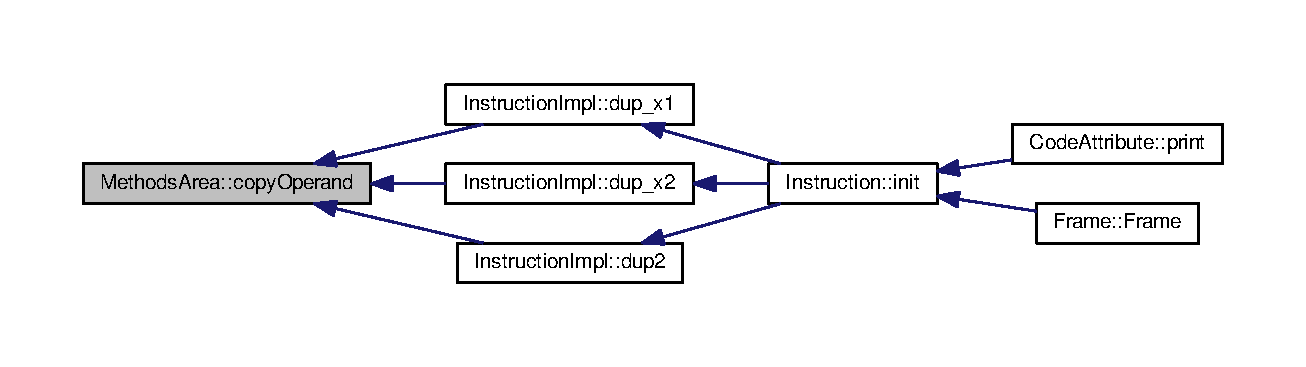
\includegraphics[width=350pt]{class_methods_area_ab4f4988ce71a130209877d841554b718_icgraph}
\end{center}
\end{figure}


\index{Methods\+Area@{Methods\+Area}!find\+Method\+By\+Name\+Or\+Deor@{find\+Method\+By\+Name\+Or\+Deor}}
\index{find\+Method\+By\+Name\+Or\+Deor@{find\+Method\+By\+Name\+Or\+Deor}!Methods\+Area@{Methods\+Area}}
\subsubsection[{\texorpdfstring{find\+Method\+By\+Name\+Or\+Deor(\+Class\+Loader $\ast$, std\+::string, std\+::string)}{findMethodByNameOrDeor(ClassLoader *, std::string, std::string)}}]{\setlength{\rightskip}{0pt plus 5cm}{\bf Method\+Info} $\ast$ Methods\+Area\+::find\+Method\+By\+Name\+Or\+Deor (
\begin{DoxyParamCaption}
\item[{{\bf Class\+Loader} $\ast$}]{classloader, }
\item[{std\+::string}]{method\+\_\+name, }
\item[{std\+::string}]{method\+\_\+desc}
\end{DoxyParamCaption}
)\hspace{0.3cm}{\ttfamily [static]}}\hypertarget{class_methods_area_ab8111f3fc9b55f1f8dbbbe0c1ca76d89}{}\label{class_methods_area_ab8111f3fc9b55f1f8dbbbe0c1ca76d89}


Grafo de chamadas desta função\+:
\nopagebreak
\begin{figure}[H]
\begin{center}
\leavevmode
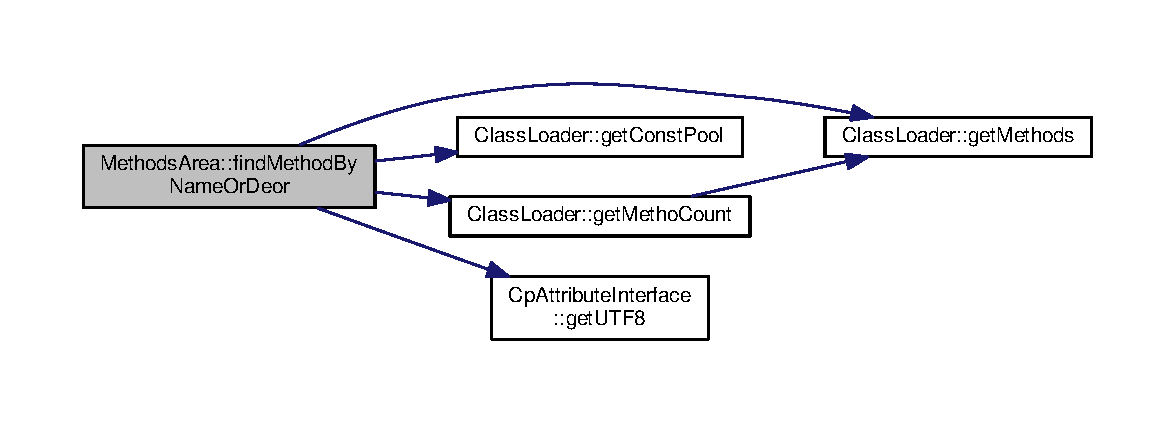
\includegraphics[width=350pt]{class_methods_area_ab8111f3fc9b55f1f8dbbbe0c1ca76d89_cgraph}
\end{center}
\end{figure}




Este é o diagrama das funções que utilizam esta função\+:
\nopagebreak
\begin{figure}[H]
\begin{center}
\leavevmode
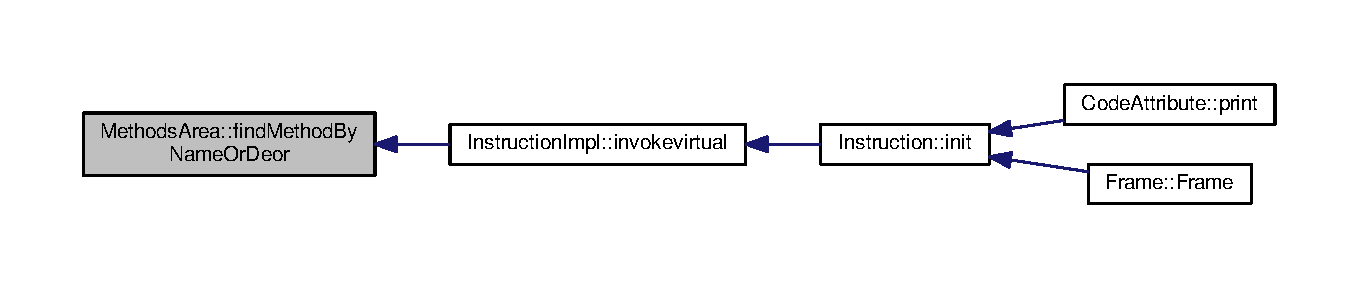
\includegraphics[width=350pt]{class_methods_area_ab8111f3fc9b55f1f8dbbbe0c1ca76d89_icgraph}
\end{center}
\end{figure}


\index{Methods\+Area@{Methods\+Area}!get\+Staticfield@{get\+Staticfield}}
\index{get\+Staticfield@{get\+Staticfield}!Methods\+Area@{Methods\+Area}}
\subsubsection[{\texorpdfstring{get\+Staticfield(std\+::string class\+Name, std\+::string var\+Name)}{getStaticfield(std::string className, std::string varName)}}]{\setlength{\rightskip}{0pt plus 5cm}{\bf Operand} $\ast$ {\bf Methods\+Area\+::get\+Staticfield} (
\begin{DoxyParamCaption}
\item[{std\+::string}]{class\+Name, }
\item[{std\+::string}]{var\+Name}
\end{DoxyParamCaption}
)\hspace{0.3cm}{\ttfamily [static]}}\hypertarget{class_methods_area_adf2c71d678e710c5fd1c357737b07f5b}{}\label{class_methods_area_adf2c71d678e710c5fd1c357737b07f5b}


Este é o diagrama das funções que utilizam esta função\+:
\nopagebreak
\begin{figure}[H]
\begin{center}
\leavevmode
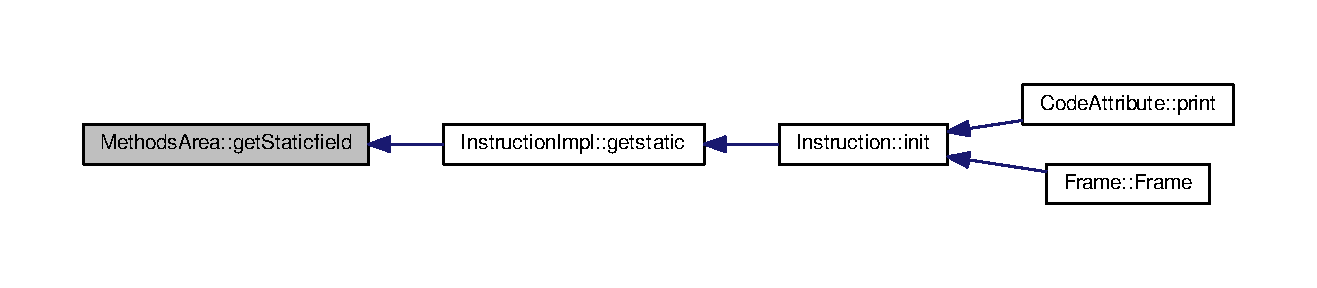
\includegraphics[width=350pt]{class_methods_area_adf2c71d678e710c5fd1c357737b07f5b_icgraph}
\end{center}
\end{figure}




\subsection{Documentação dos dados membro}
\index{Methods\+Area@{Methods\+Area}!G\+L\+O\+B\+A\+L\+\_\+loaded\+Classes@{G\+L\+O\+B\+A\+L\+\_\+loaded\+Classes}}
\index{G\+L\+O\+B\+A\+L\+\_\+loaded\+Classes@{G\+L\+O\+B\+A\+L\+\_\+loaded\+Classes}!Methods\+Area@{Methods\+Area}}
\subsubsection[{\texorpdfstring{G\+L\+O\+B\+A\+L\+\_\+loaded\+Classes}{GLOBAL_loadedClasses}}]{\setlength{\rightskip}{0pt plus 5cm}std\+::map$<$ std\+::string, {\bf Instance} $\ast$ $>$ Methods\+Area\+::\+G\+L\+O\+B\+A\+L\+\_\+loaded\+Classes\hspace{0.3cm}{\ttfamily [static]}}\hypertarget{class_methods_area_a210b48b3c45d8a2d981af099b6490438}{}\label{class_methods_area_a210b48b3c45d8a2d981af099b6490438}
\index{Methods\+Area@{Methods\+Area}!G\+L\+O\+B\+A\+L\+\_\+static\+Classes@{G\+L\+O\+B\+A\+L\+\_\+static\+Classes}}
\index{G\+L\+O\+B\+A\+L\+\_\+static\+Classes@{G\+L\+O\+B\+A\+L\+\_\+static\+Classes}!Methods\+Area@{Methods\+Area}}
\subsubsection[{\texorpdfstring{G\+L\+O\+B\+A\+L\+\_\+static\+Classes}{GLOBAL_staticClasses}}]{\setlength{\rightskip}{0pt plus 5cm}std\+::map$<$ std\+::string, {\bf Instance} $\ast$ $>$ Methods\+Area\+::\+G\+L\+O\+B\+A\+L\+\_\+static\+Classes\hspace{0.3cm}{\ttfamily [static]}}\hypertarget{class_methods_area_a34d779cc67f370a08cedc65245af2e7e}{}\label{class_methods_area_a34d779cc67f370a08cedc65245af2e7e}
\index{Methods\+Area@{Methods\+Area}!path@{path}}
\index{path@{path}!Methods\+Area@{Methods\+Area}}
\subsubsection[{\texorpdfstring{path}{path}}]{\setlength{\rightskip}{0pt plus 5cm}std\+::string Methods\+Area\+::path\hspace{0.3cm}{\ttfamily [static]}}\hypertarget{class_methods_area_af7210f4ca8ad442f7f9b83baa750b015}{}\label{class_methods_area_af7210f4ca8ad442f7f9b83baa750b015}


A documentação para esta classe foi gerada a partir dos seguintes ficheiros\+:\begin{DoxyCompactItemize}
\item 
\hyperlink{_g_l_o_b_a_l__file_8hpp}{G\+L\+O\+B\+A\+L\+\_\+file.\+hpp}\item 
\hyperlink{_g_l_o_b_a_l__file_8cpp}{G\+L\+O\+B\+A\+L\+\_\+file.\+cpp}\end{DoxyCompactItemize}

\hypertarget{class_instruction_impl_1_1monitorenter}{}\section{Referência à classe Instruction\+Impl\+:\+:monitorenter}
\label{class_instruction_impl_1_1monitorenter}\index{Instruction\+Impl\+::monitorenter@{Instruction\+Impl\+::monitorenter}}


Entra do monitor para o objeto.  




\subsection{Descrição detalhada}
Entra do monitor para o objeto. 


\begin{DoxyParams}{Parâmetros}
{\em $\ast$this\+\_\+frame} & ponteiro para o frame atual \\
\hline
\end{DoxyParams}
\begin{DoxyReturn}{Retorna}
void 
\end{DoxyReturn}


A documentação para esta classe foi gerada a partir do seguinte ficheiro\+:\begin{DoxyCompactItemize}
\item 
\hyperlink{_instruction_impl_8cpp}{Instruction\+Impl.\+cpp}\end{DoxyCompactItemize}

\hypertarget{class_instruction_impl_1_1monitorexit}{}\section{Instruction\+Impl\+:\+:monitorexit Class Reference}
\label{class_instruction_impl_1_1monitorexit}\index{Instruction\+Impl\+::monitorexit@{Instruction\+Impl\+::monitorexit}}


Sai do monitor para o objeto.  




\subsection{Detailed Description}
Sai do monitor para o objeto. 


\begin{DoxyParams}{Parameters}
{\em $\ast$this\+\_\+frame} & ponteiro para o frame atual \\
\hline
\end{DoxyParams}
\begin{DoxyReturn}{Returns}
void 
\end{DoxyReturn}


The documentation for this class was generated from the following file\+:\begin{DoxyCompactItemize}
\item 
\hyperlink{_instruction_impl_8cpp}{Instruction\+Impl.\+cpp}\end{DoxyCompactItemize}

\hypertarget{class_instruction_impl_1_1multianewarray}{}\section{Instruction\+Impl\+:\+:multianewarray Class Reference}
\label{class_instruction_impl_1_1multianewarray}\index{Instruction\+Impl\+::multianewarray@{Instruction\+Impl\+::multianewarray}}


Cria um novo array multidimensional.  




\subsection{Detailed Description}
Cria um novo array multidimensional. 


\begin{DoxyParams}{Parameters}
{\em $\ast$this\+\_\+frame} & ponteiro para o frame atual \\
\hline
\end{DoxyParams}
\begin{DoxyReturn}{Returns}
void 
\end{DoxyReturn}


The documentation for this class was generated from the following file\+:\begin{DoxyCompactItemize}
\item 
\hyperlink{_instruction_impl_8cpp}{Instruction\+Impl.\+cpp}\end{DoxyCompactItemize}

\hypertarget{class_instruction_impl_1_1new__obj}{}\section{Referência à classe Instruction\+Impl\+:\+:new\+\_\+obj}
\label{class_instruction_impl_1_1new__obj}\index{Instruction\+Impl\+::new\+\_\+obj@{Instruction\+Impl\+::new\+\_\+obj}}


Retorna long de um método.  




\subsection{Descrição detalhada}
Retorna long de um método. 


\begin{DoxyParams}{Parâmetros}
{\em $\ast$this\+\_\+frame} & ponteiro para o frame atual \\
\hline
\end{DoxyParams}
\begin{DoxyReturn}{Retorna}
void 
\end{DoxyReturn}


A documentação para esta classe foi gerada a partir do seguinte ficheiro\+:\begin{DoxyCompactItemize}
\item 
\hyperlink{_instruction_impl_8cpp}{Instruction\+Impl.\+cpp}\end{DoxyCompactItemize}

\hypertarget{class_instruction_impl_1_1newarray}{}\section{Instruction\+Impl\+:\+:newarray Class Reference}
\label{class_instruction_impl_1_1newarray}\index{Instruction\+Impl\+::newarray@{Instruction\+Impl\+::newarray}}


pega a referencia de um array, remove array, e empilha o seu tamanho no lugar  




\subsection{Detailed Description}
pega a referencia de um array, remove array, e empilha o seu tamanho no lugar 


\begin{DoxyParams}{Parameters}
{\em this\+\_\+frame} & Ponteiro para frame corrente \\
\hline
\end{DoxyParams}
\begin{DoxyReturn}{Returns}
void 
\end{DoxyReturn}


The documentation for this class was generated from the following file\+:\begin{DoxyCompactItemize}
\item 
\hyperlink{_instruction_impl_8cpp}{Instruction\+Impl.\+cpp}\end{DoxyCompactItemize}

\hypertarget{class_instruction_impl_1_1nop}{}\section{Instruction\+Impl\+:\+:nop Class Reference}
\label{class_instruction_impl_1_1nop}\index{Instruction\+Impl\+::nop@{Instruction\+Impl\+::nop}}


Incrementa o program counter.  




\subsection{Detailed Description}
Incrementa o program counter. 


\begin{DoxyParams}{Parameters}
{\em $\ast$this\+\_\+frame} & ponteiro para o frame atual \\
\hline
\end{DoxyParams}
\begin{DoxyReturn}{Returns}
void 
\end{DoxyReturn}


The documentation for this class was generated from the following file\+:\begin{DoxyCompactItemize}
\item 
\hyperlink{_instruction_impl_8cpp}{Instruction\+Impl.\+cpp}\end{DoxyCompactItemize}

\hypertarget{class_number_table_attribute}{}\section{Referência à classe Number\+Table\+Attribute}
\label{class_number_table_attribute}\index{Number\+Table\+Attribute@{Number\+Table\+Attribute}}


classe contém length e ponteiro para line\+\_\+number\+\_\+table-\/ todos uint16; Além contém métodos como leitor e print;  




{\ttfamily \#include $<$Attribute\+Info.\+hpp$>$}



Diagrama de colaboração para Number\+Table\+Attribute\+:
\nopagebreak
\begin{figure}[H]
\begin{center}
\leavevmode
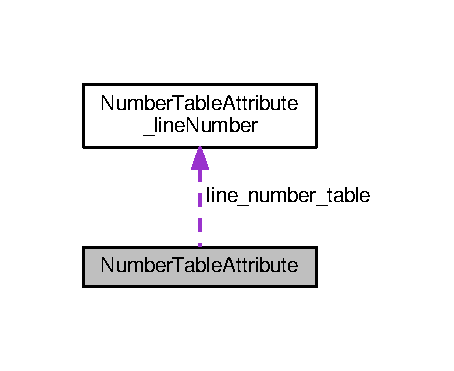
\includegraphics[width=218pt]{class_number_table_attribute__coll__graph}
\end{center}
\end{figure}
\subsection*{Componentes}
\begin{DoxyCompactItemize}
\item 
class \hyperlink{class_number_table_attribute_1_1print}{print}
\begin{DoxyCompactList}\small\item\em Print da Number\+Table dos atributos;. \end{DoxyCompactList}\item 
class \hyperlink{class_number_table_attribute_1_1read}{read}
\begin{DoxyCompactList}\small\item\em Leitor da Number\+Table dos atributos;. \end{DoxyCompactList}\end{DoxyCompactItemize}
\subsection*{Membros públicos}
\begin{DoxyCompactItemize}
\item 
void \hyperlink{class_number_table_attribute_aa56c8bbf97ea1c478e4488b93f1287a7}{read} (F\+I\+LE $\ast$)
\item 
void \hyperlink{class_number_table_attribute_a43d3c624a043ea9140c69162e3f82eaa}{print} ()
\end{DoxyCompactItemize}
\subsection*{Atributos Públicos}
\begin{DoxyCompactItemize}
\item 
uint16\+\_\+t \hyperlink{class_number_table_attribute_a5870a64b7a84529045ab1a659811f859}{length}
\item 
\hyperlink{class_number_table_attribute__line_number}{Number\+Table\+Attribute\+\_\+line\+Number} $\ast$ \hyperlink{class_number_table_attribute_ab5e3c231f1507f7be6158422eb71aeeb}{line\+\_\+number\+\_\+table}
\end{DoxyCompactItemize}


\subsection{Descrição detalhada}
classe contém length e ponteiro para line\+\_\+number\+\_\+table-\/ todos uint16; Além contém métodos como leitor e print; 

\subsection{Documentação dos métodos}
\index{Number\+Table\+Attribute@{Number\+Table\+Attribute}!print@{print}}
\index{print@{print}!Number\+Table\+Attribute@{Number\+Table\+Attribute}}
\subsubsection[{\texorpdfstring{print()}{print()}}]{\setlength{\rightskip}{0pt plus 5cm}void {\bf Number\+Table\+Attribute\+::print} (
\begin{DoxyParamCaption}
{}
\end{DoxyParamCaption}
)}\hypertarget{class_number_table_attribute_a43d3c624a043ea9140c69162e3f82eaa}{}\label{class_number_table_attribute_a43d3c624a043ea9140c69162e3f82eaa}
\index{Number\+Table\+Attribute@{Number\+Table\+Attribute}!read@{read}}
\index{read@{read}!Number\+Table\+Attribute@{Number\+Table\+Attribute}}
\subsubsection[{\texorpdfstring{read(\+F\+I\+L\+E $\ast$)}{read(FILE *)}}]{\setlength{\rightskip}{0pt plus 5cm}void {\bf Number\+Table\+Attribute\+::read} (
\begin{DoxyParamCaption}
\item[{F\+I\+LE $\ast$}]{fp}
\end{DoxyParamCaption}
)}\hypertarget{class_number_table_attribute_aa56c8bbf97ea1c478e4488b93f1287a7}{}\label{class_number_table_attribute_aa56c8bbf97ea1c478e4488b93f1287a7}


Grafo de chamadas desta função\+:
\nopagebreak
\begin{figure}[H]
\begin{center}
\leavevmode
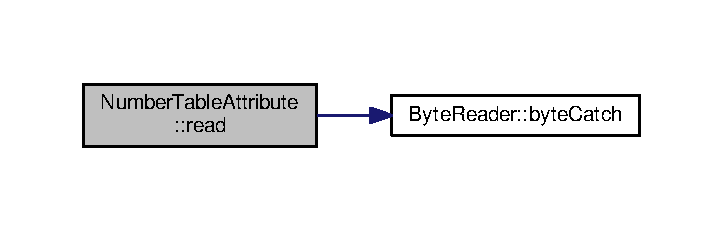
\includegraphics[width=347pt]{class_number_table_attribute_aa56c8bbf97ea1c478e4488b93f1287a7_cgraph}
\end{center}
\end{figure}




\subsection{Documentação dos dados membro}
\index{Number\+Table\+Attribute@{Number\+Table\+Attribute}!length@{length}}
\index{length@{length}!Number\+Table\+Attribute@{Number\+Table\+Attribute}}
\subsubsection[{\texorpdfstring{length}{length}}]{\setlength{\rightskip}{0pt plus 5cm}uint16\+\_\+t Number\+Table\+Attribute\+::length}\hypertarget{class_number_table_attribute_a5870a64b7a84529045ab1a659811f859}{}\label{class_number_table_attribute_a5870a64b7a84529045ab1a659811f859}
\index{Number\+Table\+Attribute@{Number\+Table\+Attribute}!line\+\_\+number\+\_\+table@{line\+\_\+number\+\_\+table}}
\index{line\+\_\+number\+\_\+table@{line\+\_\+number\+\_\+table}!Number\+Table\+Attribute@{Number\+Table\+Attribute}}
\subsubsection[{\texorpdfstring{line\+\_\+number\+\_\+table}{line_number_table}}]{\setlength{\rightskip}{0pt plus 5cm}{\bf Number\+Table\+Attribute\+\_\+line\+Number}$\ast$ Number\+Table\+Attribute\+::line\+\_\+number\+\_\+table}\hypertarget{class_number_table_attribute_ab5e3c231f1507f7be6158422eb71aeeb}{}\label{class_number_table_attribute_ab5e3c231f1507f7be6158422eb71aeeb}


A documentação para esta classe foi gerada a partir dos seguintes ficheiros\+:\begin{DoxyCompactItemize}
\item 
\hyperlink{_attribute_info_8hpp}{Attribute\+Info.\+hpp}\item 
\hyperlink{_attribute_info_8cpp}{Attribute\+Info.\+cpp}\end{DoxyCompactItemize}

\hypertarget{class_number_table_attribute__line_number}{}\section{Referência à classe Number\+Table\+Attribute\+\_\+line\+Number}
\label{class_number_table_attribute__line_number}\index{Number\+Table\+Attribute\+\_\+line\+Number@{Number\+Table\+Attribute\+\_\+line\+Number}}


classe contém strat\+\_\+pc e line\+Number -\/ todos uint16;  




{\ttfamily \#include $<$Attribute\+Info.\+hpp$>$}

\subsection*{Atributos Públicos}
\begin{DoxyCompactItemize}
\item 
uint16\+\_\+t \hyperlink{class_number_table_attribute__line_number_a2ede9887ca805349c8edc876dbc4d0da}{start\+\_\+pc}
\item 
uint16\+\_\+t \hyperlink{class_number_table_attribute__line_number_a25365848043a067fce30ee31cbfe318e}{line\+Number}
\end{DoxyCompactItemize}


\subsection{Descrição detalhada}
classe contém strat\+\_\+pc e line\+Number -\/ todos uint16; 

\subsection{Documentação dos dados membro}
\index{Number\+Table\+Attribute\+\_\+line\+Number@{Number\+Table\+Attribute\+\_\+line\+Number}!line\+Number@{line\+Number}}
\index{line\+Number@{line\+Number}!Number\+Table\+Attribute\+\_\+line\+Number@{Number\+Table\+Attribute\+\_\+line\+Number}}
\subsubsection[{\texorpdfstring{line\+Number}{lineNumber}}]{\setlength{\rightskip}{0pt plus 5cm}uint16\+\_\+t Number\+Table\+Attribute\+\_\+line\+Number\+::line\+Number}\hypertarget{class_number_table_attribute__line_number_a25365848043a067fce30ee31cbfe318e}{}\label{class_number_table_attribute__line_number_a25365848043a067fce30ee31cbfe318e}
\index{Number\+Table\+Attribute\+\_\+line\+Number@{Number\+Table\+Attribute\+\_\+line\+Number}!start\+\_\+pc@{start\+\_\+pc}}
\index{start\+\_\+pc@{start\+\_\+pc}!Number\+Table\+Attribute\+\_\+line\+Number@{Number\+Table\+Attribute\+\_\+line\+Number}}
\subsubsection[{\texorpdfstring{start\+\_\+pc}{start_pc}}]{\setlength{\rightskip}{0pt plus 5cm}uint16\+\_\+t Number\+Table\+Attribute\+\_\+line\+Number\+::start\+\_\+pc}\hypertarget{class_number_table_attribute__line_number_a2ede9887ca805349c8edc876dbc4d0da}{}\label{class_number_table_attribute__line_number_a2ede9887ca805349c8edc876dbc4d0da}


A documentação para esta classe foi gerada a partir do seguinte ficheiro\+:\begin{DoxyCompactItemize}
\item 
\hyperlink{_attribute_info_8hpp}{Attribute\+Info.\+hpp}\end{DoxyCompactItemize}

\hypertarget{struct_operand}{}\section{Referência à estrutura Operand}
\label{struct_operand}\index{Operand@{Operand}}


intuito de ligar aos tipos possíveis para variáveis que serão utilizadas;  




{\ttfamily \#include $<$Frame.\+hpp$>$}



Diagrama de colaboração para Operand\+:
\nopagebreak
\begin{figure}[H]
\begin{center}
\leavevmode
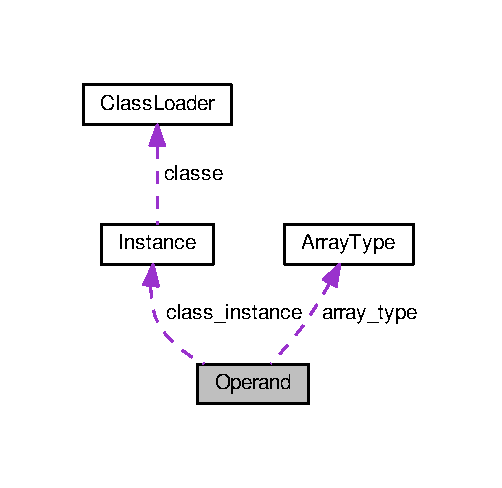
\includegraphics[width=241pt]{struct_operand__coll__graph}
\end{center}
\end{figure}
\subsection*{Atributos Públicos}
\begin{DoxyCompactItemize}
\item 
uint8\+\_\+t \hyperlink{struct_operand_a551b2888783546b27f90b70f5ceeafee}{tag}
\item 
\begin{tabbing}
xx\=xx\=xx\=xx\=xx\=xx\=xx\=xx\=xx\=\kill
union \{\\
\>uint32\_t \hyperlink{struct_operand_a0705136abc78d06866591f4a1304163b}{type\_bool}\\
\>uint32\_t \hyperlink{struct_operand_a8590d48387a47c99940dec06f4262c88}{type\_byte}\\
\>uint32\_t \hyperlink{struct_operand_a7d323bb935c240911633677c632d967b}{type\_char}\\
\>uint32\_t \hyperlink{struct_operand_a9a95367e26a5d3016da0b6d9fc9f0359}{type\_short}\\
\>uint32\_t \hyperlink{struct_operand_a5aa568fddb9132272a9c4e9870825a13}{type\_int}\\
\>uint32\_t \hyperlink{struct_operand_a323c9442608ba57c5556a67dece11c92}{type\_float}\\
\>uint64\_t \hyperlink{struct_operand_acba3d813258f86827e414fb6e6fb6963}{type\_long}\\
\>uint64\_t \hyperlink{struct_operand_a2bae1001957062fa9e95bb13a0afe2a3}{type\_double}\\
\}; \\

\end{tabbing}\item 
std\+::string $\ast$ \hyperlink{struct_operand_ab339ad43cfc3f1c32be042769846f049}{type\+\_\+string}
\item 
\hyperlink{struct_instance}{Instance} $\ast$ \hyperlink{struct_operand_a9afc0307304efd6930acb371bdabe4c2}{class\+\_\+instance}
\item 
\hyperlink{struct_array_type}{Array\+Type} $\ast$ \hyperlink{struct_operand_a79ddf8db90ba729dcee75f0f6669a8ca}{array\+\_\+type}
\end{DoxyCompactItemize}


\subsection{Descrição detalhada}
intuito de ligar aos tipos possíveis para variáveis que serão utilizadas; 

\subsection{Documentação dos dados membro}
\subsubsection[{\texorpdfstring{"@16}{@16}}]{\setlength{\rightskip}{0pt plus 5cm}union \{ ... \} }\hypertarget{struct_operand_aadc70ab04271d71be5ac82ac2a896e74}{}\label{struct_operand_aadc70ab04271d71be5ac82ac2a896e74}
\index{Operand@{Operand}!array\+\_\+type@{array\+\_\+type}}
\index{array\+\_\+type@{array\+\_\+type}!Operand@{Operand}}
\subsubsection[{\texorpdfstring{array\+\_\+type}{array_type}}]{\setlength{\rightskip}{0pt plus 5cm}{\bf Array\+Type}$\ast$ Operand\+::array\+\_\+type}\hypertarget{struct_operand_a79ddf8db90ba729dcee75f0f6669a8ca}{}\label{struct_operand_a79ddf8db90ba729dcee75f0f6669a8ca}
\index{Operand@{Operand}!class\+\_\+instance@{class\+\_\+instance}}
\index{class\+\_\+instance@{class\+\_\+instance}!Operand@{Operand}}
\subsubsection[{\texorpdfstring{class\+\_\+instance}{class_instance}}]{\setlength{\rightskip}{0pt plus 5cm}{\bf Instance}$\ast$ Operand\+::class\+\_\+instance}\hypertarget{struct_operand_a9afc0307304efd6930acb371bdabe4c2}{}\label{struct_operand_a9afc0307304efd6930acb371bdabe4c2}
\index{Operand@{Operand}!tag@{tag}}
\index{tag@{tag}!Operand@{Operand}}
\subsubsection[{\texorpdfstring{tag}{tag}}]{\setlength{\rightskip}{0pt plus 5cm}uint8\+\_\+t Operand\+::tag}\hypertarget{struct_operand_a551b2888783546b27f90b70f5ceeafee}{}\label{struct_operand_a551b2888783546b27f90b70f5ceeafee}
\index{Operand@{Operand}!type\+\_\+bool@{type\+\_\+bool}}
\index{type\+\_\+bool@{type\+\_\+bool}!Operand@{Operand}}
\subsubsection[{\texorpdfstring{type\+\_\+bool}{type_bool}}]{\setlength{\rightskip}{0pt plus 5cm}uint32\+\_\+t Operand\+::type\+\_\+bool}\hypertarget{struct_operand_a0705136abc78d06866591f4a1304163b}{}\label{struct_operand_a0705136abc78d06866591f4a1304163b}
\index{Operand@{Operand}!type\+\_\+byte@{type\+\_\+byte}}
\index{type\+\_\+byte@{type\+\_\+byte}!Operand@{Operand}}
\subsubsection[{\texorpdfstring{type\+\_\+byte}{type_byte}}]{\setlength{\rightskip}{0pt plus 5cm}uint32\+\_\+t Operand\+::type\+\_\+byte}\hypertarget{struct_operand_a8590d48387a47c99940dec06f4262c88}{}\label{struct_operand_a8590d48387a47c99940dec06f4262c88}
\index{Operand@{Operand}!type\+\_\+char@{type\+\_\+char}}
\index{type\+\_\+char@{type\+\_\+char}!Operand@{Operand}}
\subsubsection[{\texorpdfstring{type\+\_\+char}{type_char}}]{\setlength{\rightskip}{0pt plus 5cm}uint32\+\_\+t Operand\+::type\+\_\+char}\hypertarget{struct_operand_a7d323bb935c240911633677c632d967b}{}\label{struct_operand_a7d323bb935c240911633677c632d967b}
\index{Operand@{Operand}!type\+\_\+double@{type\+\_\+double}}
\index{type\+\_\+double@{type\+\_\+double}!Operand@{Operand}}
\subsubsection[{\texorpdfstring{type\+\_\+double}{type_double}}]{\setlength{\rightskip}{0pt plus 5cm}uint64\+\_\+t Operand\+::type\+\_\+double}\hypertarget{struct_operand_a2bae1001957062fa9e95bb13a0afe2a3}{}\label{struct_operand_a2bae1001957062fa9e95bb13a0afe2a3}
\index{Operand@{Operand}!type\+\_\+float@{type\+\_\+float}}
\index{type\+\_\+float@{type\+\_\+float}!Operand@{Operand}}
\subsubsection[{\texorpdfstring{type\+\_\+float}{type_float}}]{\setlength{\rightskip}{0pt plus 5cm}uint32\+\_\+t Operand\+::type\+\_\+float}\hypertarget{struct_operand_a323c9442608ba57c5556a67dece11c92}{}\label{struct_operand_a323c9442608ba57c5556a67dece11c92}
\index{Operand@{Operand}!type\+\_\+int@{type\+\_\+int}}
\index{type\+\_\+int@{type\+\_\+int}!Operand@{Operand}}
\subsubsection[{\texorpdfstring{type\+\_\+int}{type_int}}]{\setlength{\rightskip}{0pt plus 5cm}uint32\+\_\+t Operand\+::type\+\_\+int}\hypertarget{struct_operand_a5aa568fddb9132272a9c4e9870825a13}{}\label{struct_operand_a5aa568fddb9132272a9c4e9870825a13}
\index{Operand@{Operand}!type\+\_\+long@{type\+\_\+long}}
\index{type\+\_\+long@{type\+\_\+long}!Operand@{Operand}}
\subsubsection[{\texorpdfstring{type\+\_\+long}{type_long}}]{\setlength{\rightskip}{0pt plus 5cm}uint64\+\_\+t Operand\+::type\+\_\+long}\hypertarget{struct_operand_acba3d813258f86827e414fb6e6fb6963}{}\label{struct_operand_acba3d813258f86827e414fb6e6fb6963}
\index{Operand@{Operand}!type\+\_\+short@{type\+\_\+short}}
\index{type\+\_\+short@{type\+\_\+short}!Operand@{Operand}}
\subsubsection[{\texorpdfstring{type\+\_\+short}{type_short}}]{\setlength{\rightskip}{0pt plus 5cm}uint32\+\_\+t Operand\+::type\+\_\+short}\hypertarget{struct_operand_a9a95367e26a5d3016da0b6d9fc9f0359}{}\label{struct_operand_a9a95367e26a5d3016da0b6d9fc9f0359}
\index{Operand@{Operand}!type\+\_\+string@{type\+\_\+string}}
\index{type\+\_\+string@{type\+\_\+string}!Operand@{Operand}}
\subsubsection[{\texorpdfstring{type\+\_\+string}{type_string}}]{\setlength{\rightskip}{0pt plus 5cm}std\+::string$\ast$ Operand\+::type\+\_\+string}\hypertarget{struct_operand_ab339ad43cfc3f1c32be042769846f049}{}\label{struct_operand_ab339ad43cfc3f1c32be042769846f049}


A documentação para esta estrutura foi gerada a partir do seguinte ficheiro\+:\begin{DoxyCompactItemize}
\item 
\hyperlink{_frame_8hpp}{Frame.\+hpp}\end{DoxyCompactItemize}

\hypertarget{class_instruction_impl_1_1pop}{}\section{Referência à classe Instruction\+Impl\+:\+:pop}
\label{class_instruction_impl_1_1pop}\index{Instruction\+Impl\+::pop@{Instruction\+Impl\+::pop}}


Desempilha o primeiro operando da pilha.  




\subsection{Descrição detalhada}
Desempilha o primeiro operando da pilha. 


\begin{DoxyParams}{Parâmetros}
{\em $\ast$this\+\_\+frame} & Ponteiro para frame corrente. \\
\hline
\end{DoxyParams}
\begin{DoxyReturn}{Retorna}
void 
\end{DoxyReturn}


A documentação para esta classe foi gerada a partir do seguinte ficheiro\+:\begin{DoxyCompactItemize}
\item 
\hyperlink{_instruction_impl_8cpp}{Instruction\+Impl.\+cpp}\end{DoxyCompactItemize}

\hypertarget{class_instruction_impl_1_1pop2}{}\section{Instruction\+Impl\+:\+:pop2 Class Reference}
\label{class_instruction_impl_1_1pop2}\index{Instruction\+Impl\+::pop2@{Instruction\+Impl\+::pop2}}


Desempilha o primeiro e o segundo operando da pilha.  




\subsection{Detailed Description}
Desempilha o primeiro e o segundo operando da pilha. 


\begin{DoxyParams}{Parameters}
{\em $\ast$this\+\_\+frame} & Ponteiro para frame corrente. \\
\hline
\end{DoxyParams}
\begin{DoxyReturn}{Returns}
void 
\end{DoxyReturn}


The documentation for this class was generated from the following file\+:\begin{DoxyCompactItemize}
\item 
\hyperlink{_instruction_impl_8cpp}{Instruction\+Impl.\+cpp}\end{DoxyCompactItemize}

\hypertarget{class_attribute_info_1_1print}{}\section{Attribute\+Info\+:\+:print Class Reference}
\label{class_attribute_info_1_1print}\index{Attribute\+Info\+::print@{Attribute\+Info\+::print}}


É printado as informações dos atributos;.  




\subsection{Detailed Description}
É printado as informações dos atributos;. 


\begin{DoxyParams}{Parameters}
{\em fp} & arquivo .class; \\
\hline
\end{DoxyParams}
\begin{DoxyReturn}{Returns}
void; 
\end{DoxyReturn}


The documentation for this class was generated from the following file\+:\begin{DoxyCompactItemize}
\item 
\hyperlink{_attribute_info_8cpp}{Attribute\+Info.\+cpp}\end{DoxyCompactItemize}

\hypertarget{class_exception_1_1print}{}\section{Referência à classe Exception\+:\+:print}
\label{class_exception_1_1print}\index{Exception\+::print@{Exception\+::print}}


É feito o print dos number\+\_\+exceptions;.  




\subsection{Descrição detalhada}
É feito o print dos number\+\_\+exceptions;. 


\begin{DoxyParams}{Parâmetros}
{\em fp} & arquivo .class; \\
\hline
\end{DoxyParams}
\begin{DoxyReturn}{Retorna}
void; 
\end{DoxyReturn}


A documentação para esta classe foi gerada a partir do seguinte ficheiro\+:\begin{DoxyCompactItemize}
\item 
\hyperlink{_attribute_info_8cpp}{Attribute\+Info.\+cpp}\end{DoxyCompactItemize}

\hypertarget{class_code_attribute_1_1print}{}\section{Referência à classe Code\+Attribute\+:\+:print}
\label{class_code_attribute_1_1print}\index{Code\+Attribute\+::print@{Code\+Attribute\+::print}}


Print dos atributos dos methods;.  




\subsection{Descrição detalhada}
Print dos atributos dos methods;. 


\begin{DoxyParams}{Parâmetros}
{\em fp} & arquivo .class; \\
\hline
\end{DoxyParams}
\begin{DoxyReturn}{Retorna}
void; 
\end{DoxyReturn}


A documentação para esta classe foi gerada a partir do seguinte ficheiro\+:\begin{DoxyCompactItemize}
\item 
\hyperlink{_attribute_info_8cpp}{Attribute\+Info.\+cpp}\end{DoxyCompactItemize}

\hypertarget{class_constant_value_1_1print}{}\section{Constant\+Value\+:\+:print Class Reference}
\label{class_constant_value_1_1print}\index{Constant\+Value\+::print@{Constant\+Value\+::print}}


print dos valores das constantes;  




\subsection{Detailed Description}
print dos valores das constantes; 


\begin{DoxyParams}{Parameters}
{\em fp} & arquivo .class; \\
\hline
\end{DoxyParams}
\begin{DoxyReturn}{Returns}
void; 
\end{DoxyReturn}


The documentation for this class was generated from the following file\+:\begin{DoxyCompactItemize}
\item 
\hyperlink{_attribute_info_8cpp}{Attribute\+Info.\+cpp}\end{DoxyCompactItemize}

\hypertarget{class_inner_class_1_1print}{}\section{Inner\+Class\+:\+:print Class Reference}
\label{class_inner_class_1_1print}\index{Inner\+Class\+::print@{Inner\+Class\+::print}}


Print do tamanho da class;.  




\subsection{Detailed Description}
Print do tamanho da class;. 


\begin{DoxyParams}{Parameters}
{\em fp} & arquivo .class; \\
\hline
\end{DoxyParams}
\begin{DoxyReturn}{Returns}
void; 
\end{DoxyReturn}


The documentation for this class was generated from the following file\+:\begin{DoxyCompactItemize}
\item 
\hyperlink{_attribute_info_8cpp}{Attribute\+Info.\+cpp}\end{DoxyCompactItemize}

\hypertarget{class_number_table_attribute_1_1print}{}\section{Referência à classe Number\+Table\+Attribute\+:\+:print}
\label{class_number_table_attribute_1_1print}\index{Number\+Table\+Attribute\+::print@{Number\+Table\+Attribute\+::print}}


Print da Number\+Table dos atributos;.  




\subsection{Descrição detalhada}
Print da Number\+Table dos atributos;. 


\begin{DoxyParams}{Parâmetros}
{\em fp} & arquivo .class; \\
\hline
\end{DoxyParams}
\begin{DoxyReturn}{Retorna}
void; 
\end{DoxyReturn}


A documentação para esta classe foi gerada a partir do seguinte ficheiro\+:\begin{DoxyCompactItemize}
\item 
\hyperlink{_attribute_info_8cpp}{Attribute\+Info.\+cpp}\end{DoxyCompactItemize}

\hypertarget{class_instruction_impl_1_1putfield}{}\section{Referência à classe Instruction\+Impl\+:\+:putfield}
\label{class_instruction_impl_1_1putfield}\index{Instruction\+Impl\+::putfield@{Instruction\+Impl\+::putfield}}


Seta o campo em um objeto.  




\subsection{Descrição detalhada}
Seta o campo em um objeto. 


\begin{DoxyParams}{Parâmetros}
{\em $\ast$this\+\_\+frame} & ponteiro para o frame atual \\
\hline
\end{DoxyParams}
\begin{DoxyReturn}{Retorna}
void 
\end{DoxyReturn}


A documentação para esta classe foi gerada a partir do seguinte ficheiro\+:\begin{DoxyCompactItemize}
\item 
\hyperlink{_instruction_impl_8cpp}{Instruction\+Impl.\+cpp}\end{DoxyCompactItemize}

\hypertarget{class_instruction_impl_1_1putstatic}{}\section{Instruction\+Impl\+:\+:putstatic Class Reference}
\label{class_instruction_impl_1_1putstatic}\index{Instruction\+Impl\+::putstatic@{Instruction\+Impl\+::putstatic}}


Seta um static field na classe.  




\subsection{Detailed Description}
Seta um static field na classe. 


\begin{DoxyParams}{Parameters}
{\em $\ast$this\+\_\+frame} & Ponteiro para frame corrente. \\
\hline
\end{DoxyParams}
\begin{DoxyReturn}{Returns}

\end{DoxyReturn}


The documentation for this class was generated from the following file\+:\begin{DoxyCompactItemize}
\item 
\hyperlink{_instruction_impl_8cpp}{Instruction\+Impl.\+cpp}\end{DoxyCompactItemize}

\hypertarget{class_attribute_info_1_1read}{}\section{Referência à classe Attribute\+Info\+:\+:read}
\label{class_attribute_info_1_1read}\index{Attribute\+Info\+::read@{Attribute\+Info\+::read}}


É lido as informações dos atributos;.  




\subsection{Descrição detalhada}
É lido as informações dos atributos;. 


\begin{DoxyParams}{Parâmetros}
{\em fp} & arquivo .class; \\
\hline
\end{DoxyParams}
\begin{DoxyReturn}{Retorna}
void; 
\end{DoxyReturn}


A documentação para esta classe foi gerada a partir do seguinte ficheiro\+:\begin{DoxyCompactItemize}
\item 
\hyperlink{_attribute_info_8cpp}{Attribute\+Info.\+cpp}\end{DoxyCompactItemize}

\hypertarget{class_code_attribute_1_1read}{}\section{Referência à classe Code\+Attribute\+:\+:read}
\label{class_code_attribute_1_1read}\index{Code\+Attribute\+::read@{Code\+Attribute\+::read}}


Leitor dos atributos dos methods;.  




\subsection{Descrição detalhada}
Leitor dos atributos dos methods;. 


\begin{DoxyParams}{Parâmetros}
{\em fp} & arquivo .class; \\
\hline
\end{DoxyParams}
\begin{DoxyReturn}{Retorna}
void; 
\end{DoxyReturn}


A documentação para esta classe foi gerada a partir do seguinte ficheiro\+:\begin{DoxyCompactItemize}
\item 
\hyperlink{_attribute_info_8cpp}{Attribute\+Info.\+cpp}\end{DoxyCompactItemize}

\hypertarget{class_source_file_1_1read}{}\section{Referência à classe Source\+File\+:\+:read}
\label{class_source_file_1_1read}\index{Source\+File\+::read@{Source\+File\+::read}}


É lido o index do arquivo fonte;.  




\subsection{Descrição detalhada}
É lido o index do arquivo fonte;. 

É printado o index do arquivo fonte;.


\begin{DoxyParams}{Parâmetros}
{\em fp} & arquivo .class; \\
\hline
\end{DoxyParams}
\begin{DoxyReturn}{Retorna}
void; 
\end{DoxyReturn}


A documentação para esta classe foi gerada a partir do seguinte ficheiro\+:\begin{DoxyCompactItemize}
\item 
\hyperlink{_attribute_info_8cpp}{Attribute\+Info.\+cpp}\end{DoxyCompactItemize}

\hypertarget{class_constant_value_1_1read}{}\section{Constant\+Value\+:\+:read Class Reference}
\label{class_constant_value_1_1read}\index{Constant\+Value\+::read@{Constant\+Value\+::read}}


Leitor de constantes;.  




\subsection{Detailed Description}
Leitor de constantes;. 


\begin{DoxyParams}{Parameters}
{\em fp} & arquivo .class; \\
\hline
\end{DoxyParams}
\begin{DoxyReturn}{Returns}
void; 
\end{DoxyReturn}


The documentation for this class was generated from the following file\+:\begin{DoxyCompactItemize}
\item 
\hyperlink{_attribute_info_8cpp}{Attribute\+Info.\+cpp}\end{DoxyCompactItemize}

\hypertarget{class_inner_class_1_1read}{}\section{Inner\+Class\+:\+:read Class Reference}
\label{class_inner_class_1_1read}\index{Inner\+Class\+::read@{Inner\+Class\+::read}}


Leitura do tamanho da Class;.  




\subsection{Detailed Description}
Leitura do tamanho da Class;. 


\begin{DoxyParams}{Parameters}
{\em fp} & arquivo .class; \\
\hline
\end{DoxyParams}
\begin{DoxyReturn}{Returns}
void; 
\end{DoxyReturn}


The documentation for this class was generated from the following file\+:\begin{DoxyCompactItemize}
\item 
\hyperlink{_attribute_info_8cpp}{Attribute\+Info.\+cpp}\end{DoxyCompactItemize}

\hypertarget{class_cp_info_1_1read}{}\section{Cp\+Info\+:\+:read Class Reference}
\label{class_cp_info_1_1read}\index{Cp\+Info\+::read@{Cp\+Info\+::read}}


realiza o set inicial das variáveis a partir do  




\subsection{Detailed Description}
realiza o set inicial das variáveis a partir do 


\begin{DoxyParams}{Parameters}
{\em $\ast$fp} & \\
\hline
{\em $\ast$fp} & ponteiro de arquivo \\
\hline
\end{DoxyParams}
\begin{DoxyReturn}{Returns}
void 
\end{DoxyReturn}


The documentation for this class was generated from the following file\+:\begin{DoxyCompactItemize}
\item 
\hyperlink{_cp_info_8cpp}{Cp\+Info.\+cpp}\end{DoxyCompactItemize}

\hypertarget{class_number_table_attribute_1_1read}{}\section{Referência à classe Number\+Table\+Attribute\+:\+:read}
\label{class_number_table_attribute_1_1read}\index{Number\+Table\+Attribute\+::read@{Number\+Table\+Attribute\+::read}}


Leitor da Number\+Table dos atributos;.  




\subsection{Descrição detalhada}
Leitor da Number\+Table dos atributos;. 


\begin{DoxyParams}{Parâmetros}
{\em fp} & arquivo .class; \\
\hline
\end{DoxyParams}
\begin{DoxyReturn}{Retorna}
void; 
\end{DoxyReturn}


A documentação para esta classe foi gerada a partir do seguinte ficheiro\+:\begin{DoxyCompactItemize}
\item 
\hyperlink{_attribute_info_8cpp}{Attribute\+Info.\+cpp}\end{DoxyCompactItemize}

\hypertarget{class_field_info_1_1read}{}\section{Field\+Info\+:\+:read Class Reference}
\label{class_field_info_1_1read}\index{Field\+Info\+::read@{Field\+Info\+::read}}


setting inicial do \hyperlink{class_field_info}{Field\+Info} a partir de um arquivo.  




\subsection{Detailed Description}
setting inicial do \hyperlink{class_field_info}{Field\+Info} a partir de um arquivo. 


\begin{DoxyParams}{Parameters}
{\em $\ast$fp} & ponteiro de arquivo \\
\hline
{\em true\+Cp\+Info} & vetor de cp\+Info. \\
\hline
\end{DoxyParams}
\begin{DoxyReturn}{Returns}
void 
\end{DoxyReturn}


The documentation for this class was generated from the following file\+:\begin{DoxyCompactItemize}
\item 
\hyperlink{_field_info_8cpp}{Field\+Info.\+cpp}\end{DoxyCompactItemize}

\hypertarget{class_exception_1_1read}{}\section{Referência à classe Exception\+:\+:read}
\label{class_exception_1_1read}\index{Exception\+::read@{Exception\+::read}}


É feito a leitura dos number\+\_\+exceptions;.  




\subsection{Descrição detalhada}
É feito a leitura dos number\+\_\+exceptions;. 


\begin{DoxyParams}{Parâmetros}
{\em fp} & arquivo .class; \\
\hline
\end{DoxyParams}
\begin{DoxyReturn}{Retorna}
void; 
\end{DoxyReturn}


A documentação para esta classe foi gerada a partir do seguinte ficheiro\+:\begin{DoxyCompactItemize}
\item 
\hyperlink{_attribute_info_8cpp}{Attribute\+Info.\+cpp}\end{DoxyCompactItemize}

\hypertarget{class_instruction_impl_1_1ret}{}\section{Instruction\+Impl\+:\+:ret Class Reference}
\label{class_instruction_impl_1_1ret}\index{Instruction\+Impl\+::ret@{Instruction\+Impl\+::ret}}


Retorna da subrotina.  




\subsection{Detailed Description}
Retorna da subrotina. 


\begin{DoxyParams}{Parameters}
{\em $\ast$this\+\_\+frame} & ponteiro para frame atual. \\
\hline
\end{DoxyParams}
\begin{DoxyReturn}{Returns}
void 
\end{DoxyReturn}


The documentation for this class was generated from the following file\+:\begin{DoxyCompactItemize}
\item 
\hyperlink{_instruction_impl_8cpp}{Instruction\+Impl.\+cpp}\end{DoxyCompactItemize}

\hypertarget{class_frame_1_1run}{}\section{Referência à classe Frame\+:\+:run}
\label{class_frame_1_1run}\index{Frame\+::run@{Frame\+::run}}


método de execução do código armazenado em um frame.  




\subsection{Descrição detalhada}
método de execução do código armazenado em um frame. 


\begin{DoxyParams}{Parâmetros}
{\em sem} & parâmetros. \\
\hline
\end{DoxyParams}
\begin{DoxyReturn}{Retorna}
void 
\end{DoxyReturn}


A documentação para esta classe foi gerada a partir do seguinte ficheiro\+:\begin{DoxyCompactItemize}
\item 
\hyperlink{_frame_8cpp}{Frame.\+cpp}\end{DoxyCompactItemize}

\hypertarget{class_instruction_impl_1_1saload}{}\section{Instruction\+Impl\+:\+:saload Class Reference}
\label{class_instruction_impl_1_1saload}\index{Instruction\+Impl\+::saload@{Instruction\+Impl\+::saload}}


Empilha na pilha de operandos um char de um array de chars.  




\subsection{Detailed Description}
Empilha na pilha de operandos um char de um array de chars. 


\begin{DoxyParams}{Parameters}
{\em $\ast$this\+\_\+frame} & Ponteiro para o frame atual \\
\hline
\end{DoxyParams}
\begin{DoxyReturn}{Returns}
void 
\end{DoxyReturn}


The documentation for this class was generated from the following file\+:\begin{DoxyCompactItemize}
\item 
\hyperlink{_instruction_impl_8cpp}{Instruction\+Impl.\+cpp}\end{DoxyCompactItemize}

\hypertarget{class_instruction_impl_1_1sastore}{}\section{Instruction\+Impl\+:\+:sastore Class Reference}
\label{class_instruction_impl_1_1sastore}\index{Instruction\+Impl\+::sastore@{Instruction\+Impl\+::sastore}}


Desempilha a referencia para o array, o indice e o valor(short) e salva o valor no array. Trunca int do stack para short de 16 bits.  




\subsection{Detailed Description}
Desempilha a referencia para o array, o indice e o valor(short) e salva o valor no array. Trunca int do stack para short de 16 bits. 


\begin{DoxyParams}{Parameters}
{\em $\ast$this\+\_\+frame} & Ponteiro para frame corrente. \\
\hline
\end{DoxyParams}
\begin{DoxyReturn}{Returns}
void 
\end{DoxyReturn}


The documentation for this class was generated from the following file\+:\begin{DoxyCompactItemize}
\item 
\hyperlink{_instruction_impl_8cpp}{Instruction\+Impl.\+cpp}\end{DoxyCompactItemize}

\hypertarget{class_class_loader_1_1set_access_flag}{}\section{Referência à classe Class\+Loader\+:\+:set\+Access\+Flag}
\label{class_class_loader_1_1set_access_flag}\index{Class\+Loader\+::set\+Access\+Flag@{Class\+Loader\+::set\+Access\+Flag}}


O valor setado através desse método é uma mascara de flags que denotam o acesso das propriedades da classe ou interface;.  




\subsection{Descrição detalhada}
O valor setado através desse método é uma mascara de flags que denotam o acesso das propriedades da classe ou interface;. 


\begin{DoxyParams}{Parâmetros}
{\em Arquivo} & .class \\
\hline
\end{DoxyParams}
\begin{DoxyReturn}{Retorna}
void; 
\end{DoxyReturn}


A documentação para esta classe foi gerada a partir do seguinte ficheiro\+:\begin{DoxyCompactItemize}
\item 
\hyperlink{_class_loader_8cpp}{Class\+Loader.\+cpp}\end{DoxyCompactItemize}

\hypertarget{class_class_loader_1_1set_attributes}{}\section{Referência à classe Class\+Loader\+:\+:set\+Attributes}
\label{class_class_loader_1_1set_attributes}\index{Class\+Loader\+::set\+Attributes@{Class\+Loader\+::set\+Attributes}}


Método que seta uma array de attribute\+\_\+info ;.  




\subsection{Descrição detalhada}
Método que seta uma array de attribute\+\_\+info ;. 


\begin{DoxyParams}{Parâmetros}
{\em Arquivo} & .class \\
\hline
\end{DoxyParams}
\begin{DoxyReturn}{Retorna}
void; 
\end{DoxyReturn}


A documentação para esta classe foi gerada a partir do seguinte ficheiro\+:\begin{DoxyCompactItemize}
\item 
\hyperlink{_class_loader_8cpp}{Class\+Loader.\+cpp}\end{DoxyCompactItemize}

\hypertarget{class_class_loader_1_1set_attributes_count}{}\section{Referência à classe Class\+Loader\+:\+:set\+Attributes\+Count}
\label{class_class_loader_1_1set_attributes_count}\index{Class\+Loader\+::set\+Attributes\+Count@{Class\+Loader\+::set\+Attributes\+Count}}


Método que seta a quantidade de estruturas attribute\+\_\+info ;.  




\subsection{Descrição detalhada}
Método que seta a quantidade de estruturas attribute\+\_\+info ;. 


\begin{DoxyParams}{Parâmetros}
{\em Arquivo} & .class \\
\hline
\end{DoxyParams}
\begin{DoxyReturn}{Retorna}
void; 
\end{DoxyReturn}


A documentação para esta classe foi gerada a partir do seguinte ficheiro\+:\begin{DoxyCompactItemize}
\item 
\hyperlink{_class_loader_8cpp}{Class\+Loader.\+cpp}\end{DoxyCompactItemize}

\hypertarget{class_class_loader_1_1set_const_count}{}\section{Class\+Loader\+:\+:set\+Const\+Count Class Reference}
\label{class_class_loader_1_1set_const_count}\index{Class\+Loader\+::set\+Const\+Count@{Class\+Loader\+::set\+Const\+Count}}


Método com o objetivo de setar a quantidade de constant pool mais 1;.  




\subsection{Detailed Description}
Método com o objetivo de setar a quantidade de constant pool mais 1;. 


\begin{DoxyParams}{Parameters}
{\em Arquivo} & .class \\
\hline
\end{DoxyParams}
\begin{DoxyReturn}{Returns}
void; 
\end{DoxyReturn}


The documentation for this class was generated from the following file\+:\begin{DoxyCompactItemize}
\item 
\hyperlink{_class_loader_8cpp}{Class\+Loader.\+cpp}\end{DoxyCompactItemize}

\hypertarget{class_class_loader_1_1set_const_pool}{}\section{Class\+Loader\+:\+:set\+Const\+Pool Class Reference}
\label{class_class_loader_1_1set_const_pool}\index{Class\+Loader\+::set\+Const\+Pool@{Class\+Loader\+::set\+Const\+Pool}}


Método com o objetivo de representar uma tebela de estruturas como strings, classes, interfaces, entre outros; O formato para cada constant pool na tabela é indicado com uma tag;.  




\subsection{Detailed Description}
Método com o objetivo de representar uma tebela de estruturas como strings, classes, interfaces, entre outros; O formato para cada constant pool na tabela é indicado com uma tag;. 


\begin{DoxyParams}{Parameters}
{\em Arquivo} & .class \\
\hline
\end{DoxyParams}
\begin{DoxyReturn}{Returns}
void; 
\end{DoxyReturn}


The documentation for this class was generated from the following file\+:\begin{DoxyCompactItemize}
\item 
\hyperlink{_class_loader_8cpp}{Class\+Loader.\+cpp}\end{DoxyCompactItemize}

\hypertarget{class_class_loader_1_1set_field_count}{}\section{Referência à classe Class\+Loader\+:\+:set\+Field\+Count}
\label{class_class_loader_1_1set_field_count}\index{Class\+Loader\+::set\+Field\+Count@{Class\+Loader\+::set\+Field\+Count}}


Método com o objetivo de setar a quantidade de estruturas do tipo field\+\_\+info na tabela de fields ;.  




\subsection{Descrição detalhada}
Método com o objetivo de setar a quantidade de estruturas do tipo field\+\_\+info na tabela de fields ;. 


\begin{DoxyParams}{Parâmetros}
{\em Arquivo} & .class \\
\hline
\end{DoxyParams}
\begin{DoxyReturn}{Retorna}
void; 
\end{DoxyReturn}


A documentação para esta classe foi gerada a partir do seguinte ficheiro\+:\begin{DoxyCompactItemize}
\item 
\hyperlink{_class_loader_8cpp}{Class\+Loader.\+cpp}\end{DoxyCompactItemize}

\hypertarget{class_class_loader_1_1set_fields}{}\section{Referência à classe Class\+Loader\+:\+:set\+Fields}
\label{class_class_loader_1_1set_fields}\index{Class\+Loader\+::set\+Fields@{Class\+Loader\+::set\+Fields}}


Método que seta uma array de field\+\_\+info ;.  




\subsection{Descrição detalhada}
Método que seta uma array de field\+\_\+info ;. 


\begin{DoxyParams}{Parâmetros}
{\em Arquivo} & .class \\
\hline
\end{DoxyParams}
\begin{DoxyReturn}{Retorna}
void; 
\end{DoxyReturn}


A documentação para esta classe foi gerada a partir do seguinte ficheiro\+:\begin{DoxyCompactItemize}
\item 
\hyperlink{_class_loader_8cpp}{Class\+Loader.\+cpp}\end{DoxyCompactItemize}

\hypertarget{class_class_loader_1_1set_inter_count}{}\section{Referência à classe Class\+Loader\+:\+:set\+Inter\+Count}
\label{class_class_loader_1_1set_inter_count}\index{Class\+Loader\+::set\+Inter\+Count@{Class\+Loader\+::set\+Inter\+Count}}


Método que seta a quantidade de superinterfaces e tipo interface;.  




\subsection{Descrição detalhada}
Método que seta a quantidade de superinterfaces e tipo interface;. 


\begin{DoxyParams}{Parâmetros}
{\em Arquivo} & .class \\
\hline
\end{DoxyParams}
\begin{DoxyReturn}{Retorna}
void; 
\end{DoxyReturn}


A documentação para esta classe foi gerada a partir do seguinte ficheiro\+:\begin{DoxyCompactItemize}
\item 
\hyperlink{_class_loader_8cpp}{Class\+Loader.\+cpp}\end{DoxyCompactItemize}

\hypertarget{class_class_loader_1_1set_interface}{}\section{Class\+Loader\+:\+:set\+Interface Class Reference}
\label{class_class_loader_1_1set_interface}\index{Class\+Loader\+::set\+Interface@{Class\+Loader\+::set\+Interface}}


Método que seta uma array contendo as interfaces pegas a partir de index válidos no contant\+\_\+poll;.  




\subsection{Detailed Description}
Método que seta uma array contendo as interfaces pegas a partir de index válidos no contant\+\_\+poll;. 


\begin{DoxyParams}{Parameters}
{\em Arquivo} & .class \\
\hline
\end{DoxyParams}
\begin{DoxyReturn}{Returns}
void; 
\end{DoxyReturn}


The documentation for this class was generated from the following file\+:\begin{DoxyCompactItemize}
\item 
\hyperlink{_class_loader_8cpp}{Class\+Loader.\+cpp}\end{DoxyCompactItemize}

\hypertarget{class_interface_info_1_1set_interface_info}{}\section{Referência à classe Interface\+Info\+:\+:set\+Interface\+Info}
\label{class_interface_info_1_1set_interface_info}\index{Interface\+Info\+::set\+Interface\+Info@{Interface\+Info\+::set\+Interface\+Info}}


Carrega as informações de um arquivo na instância de \hyperlink{class_interface_info}{Interface\+Info}.  




\subsection{Descrição detalhada}
Carrega as informações de um arquivo na instância de \hyperlink{class_interface_info}{Interface\+Info}. 


\begin{DoxyParams}{Parâmetros}
{\em $\ast$fp} & ponteiro de arquivo \\
\hline
\end{DoxyParams}
\begin{DoxyReturn}{Retorna}
void 
\end{DoxyReturn}


A documentação para esta classe foi gerada a partir do seguinte ficheiro\+:\begin{DoxyCompactItemize}
\item 
\hyperlink{_interface_info_8cpp}{Interface\+Info.\+cpp}\end{DoxyCompactItemize}

\hypertarget{class_class_loader_1_1set_magic}{}\section{Class\+Loader\+:\+:set\+Magic Class Reference}
\label{class_class_loader_1_1set_magic}\index{Class\+Loader\+::set\+Magic@{Class\+Loader\+::set\+Magic}}


Método que busca identificar o formato da classe. Tem o valor de 0x\+C\+A\+F\+E\+B\+A\+BE;.  




\subsection{Detailed Description}
Método que busca identificar o formato da classe. Tem o valor de 0x\+C\+A\+F\+E\+B\+A\+BE;. 


\begin{DoxyParams}{Parameters}
{\em Arquivo} & .class \\
\hline
\end{DoxyParams}
\begin{DoxyReturn}{Returns}
void; 
\end{DoxyReturn}


The documentation for this class was generated from the following file\+:\begin{DoxyCompactItemize}
\item 
\hyperlink{_class_loader_8cpp}{Class\+Loader.\+cpp}\end{DoxyCompactItemize}

\hypertarget{class_class_loader_1_1set_major}{}\section{Class\+Loader\+:\+:set\+Major Class Reference}
\label{class_class_loader_1_1set_major}\index{Class\+Loader\+::set\+Major@{Class\+Loader\+::set\+Major}}


Método como Major busca identificar a maior versão acessivel do formato do arquivo de classe;.  




\subsection{Detailed Description}
Método como Major busca identificar a maior versão acessivel do formato do arquivo de classe;. 


\begin{DoxyParams}{Parameters}
{\em Arquivo} & .class \\
\hline
\end{DoxyParams}
\begin{DoxyReturn}{Returns}
void; 
\end{DoxyReturn}


The documentation for this class was generated from the following file\+:\begin{DoxyCompactItemize}
\item 
\hyperlink{_class_loader_8cpp}{Class\+Loader.\+cpp}\end{DoxyCompactItemize}

\hypertarget{class_class_loader_1_1set_method_count}{}\section{Referência à classe Class\+Loader\+:\+:set\+Method\+Count}
\label{class_class_loader_1_1set_method_count}\index{Class\+Loader\+::set\+Method\+Count@{Class\+Loader\+::set\+Method\+Count}}


Método seta a quantidade de estruturas method\+\_\+info ;.  




\subsection{Descrição detalhada}
Método seta a quantidade de estruturas method\+\_\+info ;. 


\begin{DoxyParams}{Parâmetros}
{\em Arquivo} & .class \\
\hline
\end{DoxyParams}
\begin{DoxyReturn}{Retorna}
void; 
\end{DoxyReturn}


A documentação para esta classe foi gerada a partir do seguinte ficheiro\+:\begin{DoxyCompactItemize}
\item 
\hyperlink{_class_loader_8cpp}{Class\+Loader.\+cpp}\end{DoxyCompactItemize}

\hypertarget{class_class_loader_1_1set_methods}{}\section{Class\+Loader\+:\+:set\+Methods Class Reference}
\label{class_class_loader_1_1set_methods}\index{Class\+Loader\+::set\+Methods@{Class\+Loader\+::set\+Methods}}


Método que seta uma array de methods\+\_\+info ;.  




\subsection{Detailed Description}
Método que seta uma array de methods\+\_\+info ;. 


\begin{DoxyParams}{Parameters}
{\em Arquivo} & .class \\
\hline
\end{DoxyParams}
\begin{DoxyReturn}{Returns}
void; 
\end{DoxyReturn}


The documentation for this class was generated from the following file\+:\begin{DoxyCompactItemize}
\item 
\hyperlink{_class_loader_8cpp}{Class\+Loader.\+cpp}\end{DoxyCompactItemize}

\hypertarget{class_class_loader_1_1set_minor}{}\section{Referência à classe Class\+Loader\+:\+:set\+Minor}
\label{class_class_loader_1_1set_minor}\index{Class\+Loader\+::set\+Minor@{Class\+Loader\+::set\+Minor}}


Método como Minor busca identificar a menor versão acessivel do formato do arquivo de classe;.  




\subsection{Descrição detalhada}
Método como Minor busca identificar a menor versão acessivel do formato do arquivo de classe;. 


\begin{DoxyParams}{Parâmetros}
{\em Arquivo} & .class \\
\hline
\end{DoxyParams}
\begin{DoxyReturn}{Retorna}
void; 
\end{DoxyReturn}


A documentação para esta classe foi gerada a partir do seguinte ficheiro\+:\begin{DoxyCompactItemize}
\item 
\hyperlink{_class_loader_8cpp}{Class\+Loader.\+cpp}\end{DoxyCompactItemize}

\hypertarget{class_class_loader_1_1set_super_class}{}\section{Referência à classe Class\+Loader\+:\+:set\+Super\+Class}
\label{class_class_loader_1_1set_super_class}\index{Class\+Loader\+::set\+Super\+Class@{Class\+Loader\+::set\+Super\+Class}}


Caso o valor do index passado seja diferente de zero, é tratado como uma C\+O\+N\+S\+T\+A\+N\+T\+\_\+\+Class\+\_\+info, caso contrário é tratado como objeto;.  




\subsection{Descrição detalhada}
Caso o valor do index passado seja diferente de zero, é tratado como uma C\+O\+N\+S\+T\+A\+N\+T\+\_\+\+Class\+\_\+info, caso contrário é tratado como objeto;. 


\begin{DoxyParams}{Parâmetros}
{\em Arquivo} & .class \\
\hline
\end{DoxyParams}
\begin{DoxyReturn}{Retorna}
void; 
\end{DoxyReturn}


A documentação para esta classe foi gerada a partir do seguinte ficheiro\+:\begin{DoxyCompactItemize}
\item 
\hyperlink{_class_loader_8cpp}{Class\+Loader.\+cpp}\end{DoxyCompactItemize}

\hypertarget{class_class_loader_1_1set_this_class}{}\section{Class\+Loader\+:\+:set\+This\+Class Class Reference}
\label{class_class_loader_1_1set_this_class}\index{Class\+Loader\+::set\+This\+Class@{Class\+Loader\+::set\+This\+Class}}


Método que seta um index valido pego da tabela de constatnt pool que indica uma C\+O\+N\+S\+T\+A\+N\+T\+\_\+\+Class\+\_\+info;.  




\subsection{Detailed Description}
Método que seta um index valido pego da tabela de constatnt pool que indica uma C\+O\+N\+S\+T\+A\+N\+T\+\_\+\+Class\+\_\+info;. 


\begin{DoxyParams}{Parameters}
{\em Arquivo} & .class \\
\hline
\end{DoxyParams}
\begin{DoxyReturn}{Returns}
void; 
\end{DoxyReturn}


The documentation for this class was generated from the following file\+:\begin{DoxyCompactItemize}
\item 
\hyperlink{_class_loader_8cpp}{Class\+Loader.\+cpp}\end{DoxyCompactItemize}

\hypertarget{class_instruction_impl_1_1sipush}{}\section{Referência à classe Instruction\+Impl\+:\+:sipush}
\label{class_instruction_impl_1_1sipush}\index{Instruction\+Impl\+::sipush@{Instruction\+Impl\+::sipush}}


Empilha int composto por byte de argumento na pilha de operandos.  




\subsection{Descrição detalhada}
Empilha int composto por byte de argumento na pilha de operandos. 


\begin{DoxyParams}{Parâmetros}
{\em $\ast$this\+\_\+frame} & Ponteiro para o frame atual \\
\hline
\end{DoxyParams}
\begin{DoxyReturn}{Retorna}
void 
\end{DoxyReturn}


A documentação para esta classe foi gerada a partir do seguinte ficheiro\+:\begin{DoxyCompactItemize}
\item 
\hyperlink{_instruction_impl_8cpp}{Instruction\+Impl.\+cpp}\end{DoxyCompactItemize}

\hypertarget{class_source_file}{}\section{Source\+File Class Reference}
\label{class_source_file}\index{Source\+File@{Source\+File}}


classe contém source\+File\+Index -\/ todos uint16; Além contém métodos como leitor e print;  




{\ttfamily \#include $<$Attribute\+Info.\+hpp$>$}

\subsection*{Classes}
\begin{DoxyCompactItemize}
\item 
class \hyperlink{class_source_file_1_1read}{read}
\begin{DoxyCompactList}\small\item\em É lido o index do arquivo fonte;. \end{DoxyCompactList}\end{DoxyCompactItemize}
\subsection*{Public Member Functions}
\begin{DoxyCompactItemize}
\item 
void \hyperlink{class_source_file_ab03dce42dd5c3f890ac4efa38e9d93e6}{read} (F\+I\+LE $\ast$)
\item 
void \hyperlink{class_source_file_ab60e06ebfcc9d1c9d0dda817cca0fc10}{print} (std\+::vector$<$ \hyperlink{class_cp_info}{Cp\+Info} $\ast$ $>$)
\end{DoxyCompactItemize}
\subsection*{Public Attributes}
\begin{DoxyCompactItemize}
\item 
uint16\+\_\+t \hyperlink{class_source_file_a3786d0b21d98b8fe5cd7ca9840a12975}{source\+File\+Index}
\end{DoxyCompactItemize}


\subsection{Detailed Description}
classe contém source\+File\+Index -\/ todos uint16; Além contém métodos como leitor e print; 

\subsection{Member Function Documentation}
\index{Source\+File@{Source\+File}!print@{print}}
\index{print@{print}!Source\+File@{Source\+File}}
\subsubsection[{\texorpdfstring{print(std\+::vector$<$ Cp\+Info $\ast$ $>$)}{print(std::vector< CpInfo * >)}}]{\setlength{\rightskip}{0pt plus 5cm}void Source\+File\+::print (
\begin{DoxyParamCaption}
\item[{std\+::vector$<$ {\bf Cp\+Info} $\ast$ $>$}]{true\+Cp\+Info}
\end{DoxyParamCaption}
)}\hypertarget{class_source_file_ab60e06ebfcc9d1c9d0dda817cca0fc10}{}\label{class_source_file_ab60e06ebfcc9d1c9d0dda817cca0fc10}


Here is the call graph for this function\+:
% FIG 0


\index{Source\+File@{Source\+File}!read@{read}}
\index{read@{read}!Source\+File@{Source\+File}}
\subsubsection[{\texorpdfstring{read(\+F\+I\+L\+E $\ast$)}{read(FILE *)}}]{\setlength{\rightskip}{0pt plus 5cm}void {\bf Source\+File\+::read} (
\begin{DoxyParamCaption}
\item[{F\+I\+LE $\ast$}]{fp}
\end{DoxyParamCaption}
)}\hypertarget{class_source_file_ab03dce42dd5c3f890ac4efa38e9d93e6}{}\label{class_source_file_ab03dce42dd5c3f890ac4efa38e9d93e6}


Here is the call graph for this function\+:
% FIG 1




\subsection{Member Data Documentation}
\index{Source\+File@{Source\+File}!source\+File\+Index@{source\+File\+Index}}
\index{source\+File\+Index@{source\+File\+Index}!Source\+File@{Source\+File}}
\subsubsection[{\texorpdfstring{source\+File\+Index}{sourceFileIndex}}]{\setlength{\rightskip}{0pt plus 5cm}uint16\+\_\+t Source\+File\+::source\+File\+Index}\hypertarget{class_source_file_a3786d0b21d98b8fe5cd7ca9840a12975}{}\label{class_source_file_a3786d0b21d98b8fe5cd7ca9840a12975}


The documentation for this class was generated from the following files\+:\begin{DoxyCompactItemize}
\item 
\hyperlink{_attribute_info_8hpp}{Attribute\+Info.\+hpp}\item 
\hyperlink{_attribute_info_8cpp}{Attribute\+Info.\+cpp}\end{DoxyCompactItemize}

\hypertarget{class_instruction_impl_1_1swap}{}\section{Instruction\+Impl\+:\+:swap Class Reference}
\label{class_instruction_impl_1_1swap}\index{Instruction\+Impl\+::swap@{Instruction\+Impl\+::swap}}


Realiza uma permutação entre os 2 primeiros elementos da pilha.  




\subsection{Detailed Description}
Realiza uma permutação entre os 2 primeiros elementos da pilha. 


\begin{DoxyParams}{Parameters}
{\em $\ast$thisframe} & ponteiro para o frame. \\
\hline
\end{DoxyParams}
\begin{DoxyReturn}{Returns}
void 
\end{DoxyReturn}


The documentation for this class was generated from the following file\+:\begin{DoxyCompactItemize}
\item 
\hyperlink{_instruction_impl_8cpp}{Instruction\+Impl.\+cpp}\end{DoxyCompactItemize}

\hypertarget{class_instruction_impl_1_1tableswitch}{}\section{Referência à classe Instruction\+Impl\+:\+:tableswitch}
\label{class_instruction_impl_1_1tableswitch}\index{Instruction\+Impl\+::tableswitch@{Instruction\+Impl\+::tableswitch}}


Acessa o jump table pelo index e executa o jump.  




\subsection{Descrição detalhada}
Acessa o jump table pelo index e executa o jump. 


\begin{DoxyParams}{Parâmetros}
{\em $\ast$this\+\_\+frame} & ponteiro para frame atual. \\
\hline
\end{DoxyParams}
\begin{DoxyReturn}{Retorna}
void 
\end{DoxyReturn}


A documentação para esta classe foi gerada a partir do seguinte ficheiro\+:\begin{DoxyCompactItemize}
\item 
\hyperlink{_instruction_impl_8cpp}{Instruction\+Impl.\+cpp}\end{DoxyCompactItemize}

\hypertarget{class_instruction_impl_1_1void__return}{}\section{Instruction\+Impl\+:\+:void\+\_\+return Class Reference}
\label{class_instruction_impl_1_1void__return}\index{Instruction\+Impl\+::void\+\_\+return@{Instruction\+Impl\+::void\+\_\+return}}


Retorna void do metodo.  




\subsection{Detailed Description}
Retorna void do metodo. 


\begin{DoxyParams}{Parameters}
{\em $\ast$this\+\_\+frame} & ponteiro para o frame atual \\
\hline
\end{DoxyParams}
\begin{DoxyReturn}{Returns}
void 
\end{DoxyReturn}


The documentation for this class was generated from the following file\+:\begin{DoxyCompactItemize}
\item 
\hyperlink{_instruction_impl_8cpp}{Instruction\+Impl.\+cpp}\end{DoxyCompactItemize}

\hypertarget{class_instruction_impl_1_1wide}{}\section{Referência à classe Instruction\+Impl\+:\+:wide}
\label{class_instruction_impl_1_1wide}\index{Instruction\+Impl\+::wide@{Instruction\+Impl\+::wide}}


Extende um local para adicionar os bytes.  




\subsection{Descrição detalhada}
Extende um local para adicionar os bytes. 


\begin{DoxyParams}{Parâmetros}
{\em $\ast$this\+\_\+frame} & ponteiro para o frame atual \\
\hline
\end{DoxyParams}
\begin{DoxyReturn}{Retorna}
void 
\end{DoxyReturn}


A documentação para esta classe foi gerada a partir do seguinte ficheiro\+:\begin{DoxyCompactItemize}
\item 
\hyperlink{_instruction_impl_8cpp}{Instruction\+Impl.\+cpp}\end{DoxyCompactItemize}

\hypertarget{class_attribute_info_1_1~_attribute_info}{}\section{Attribute\+Info\+:\+:$\sim$\+Attribute\+Info Class Reference}
\label{class_attribute_info_1_1~_attribute_info}\index{Attribute\+Info\+::````~Attribute\+Info@{Attribute\+Info\+::$\sim$\+Attribute\+Info}}


Destrutor Attribute\+\_\+info.  




\subsection{Detailed Description}
Destrutor Attribute\+\_\+info. 

The documentation for this class was generated from the following file\+:\begin{DoxyCompactItemize}
\item 
\hyperlink{_attribute_info_8cpp}{Attribute\+Info.\+cpp}\end{DoxyCompactItemize}

\hypertarget{class_class_loader_1_1~_class_loader}{}\section{Referência à classe Class\+Loader\+:\+:$\sim$\+Class\+Loader}
\label{class_class_loader_1_1~_class_loader}\index{Class\+Loader\+::````~Class\+Loader@{Class\+Loader\+::$\sim$\+Class\+Loader}}


Aqui são feitas as desalocações da \hyperlink{class_class_loader_1_1_class_loader}{Class\+Loader};.  




\subsection{Descrição detalhada}
Aqui são feitas as desalocações da \hyperlink{class_class_loader_1_1_class_loader}{Class\+Loader};. 


\begin{DoxyParams}{Parâmetros}
{\em fp} & = destructor; \\
\hline
\end{DoxyParams}
\begin{DoxyReturn}{Retorna}
destructor; 
\end{DoxyReturn}


A documentação para esta classe foi gerada a partir do seguinte ficheiro\+:\begin{DoxyCompactItemize}
\item 
\hyperlink{_class_loader_8cpp}{Class\+Loader.\+cpp}\end{DoxyCompactItemize}

\hypertarget{class_code_attribute_1_1~_code_attribute}{}\section{Code\+Attribute\+:\+:$\sim$\+Code\+Attribute Class Reference}
\label{class_code_attribute_1_1~_code_attribute}\index{Code\+Attribute\+::````~Code\+Attribute@{Code\+Attribute\+::$\sim$\+Code\+Attribute}}


Destrutor \hyperlink{class_code_attribute}{Code\+Attribute}.  




\subsection{Detailed Description}
Destrutor \hyperlink{class_code_attribute}{Code\+Attribute}. 

The documentation for this class was generated from the following file\+:\begin{DoxyCompactItemize}
\item 
\hyperlink{_attribute_info_8cpp}{Attribute\+Info.\+cpp}\end{DoxyCompactItemize}

\hypertarget{class_cp_info_1_1~_cp_info}{}\section{Cp\+Info\+:\+:$\sim$\+Cp\+Info Class Reference}
\label{class_cp_info_1_1~_cp_info}\index{Cp\+Info\+::````~Cp\+Info@{Cp\+Info\+::$\sim$\+Cp\+Info}}


Destrutor de \hyperlink{class_cp_info}{Cp\+Info}, desaloca o que foi alocado.  




\subsection{Detailed Description}
Destrutor de \hyperlink{class_cp_info}{Cp\+Info}, desaloca o que foi alocado. 


\begin{DoxyParams}{Parameters}
{\em sem} & parâmetros \\
\hline
\end{DoxyParams}
\begin{DoxyReturn}{Returns}
void 
\end{DoxyReturn}


The documentation for this class was generated from the following file\+:\begin{DoxyCompactItemize}
\item 
\hyperlink{_cp_info_8cpp}{Cp\+Info.\+cpp}\end{DoxyCompactItemize}

\hypertarget{class_exception_1_1~_exception}{}\section{Referência à classe Exception\+:\+:$\sim$\+Exception}
\label{class_exception_1_1~_exception}\index{Exception\+::````~Exception@{Exception\+::$\sim$\+Exception}}


Destrutor exception\+\_\+index\+\_\+table.  




\subsection{Descrição detalhada}
Destrutor exception\+\_\+index\+\_\+table. 

A documentação para esta classe foi gerada a partir do seguinte ficheiro\+:\begin{DoxyCompactItemize}
\item 
\hyperlink{_attribute_info_8cpp}{Attribute\+Info.\+cpp}\end{DoxyCompactItemize}

\hypertarget{class_field_info_1_1~_field_info}{}\section{Field\+Info\+:\+:$\sim$\+Field\+Info Class Reference}
\label{class_field_info_1_1~_field_info}\index{Field\+Info\+::````~Field\+Info@{Field\+Info\+::$\sim$\+Field\+Info}}


Destrutor de \hyperlink{class_field_info}{Field\+Info}.  




\subsection{Detailed Description}
Destrutor de \hyperlink{class_field_info}{Field\+Info}. 


\begin{DoxyParams}{Parameters}
{\em sem} & parâmetros. \\
\hline
\end{DoxyParams}
\begin{DoxyReturn}{Returns}
void 
\end{DoxyReturn}


The documentation for this class was generated from the following file\+:\begin{DoxyCompactItemize}
\item 
\hyperlink{_field_info_8cpp}{Field\+Info.\+cpp}\end{DoxyCompactItemize}

\hypertarget{class_frame_1_1~_frame}{}\section{Frame\+:\+:$\sim$\+Frame Class Reference}
\label{class_frame_1_1~_frame}\index{Frame\+::````~Frame@{Frame\+::$\sim$\+Frame}}


Destrutor de frame, libera o que é alocado no construtor de frame.  




\subsection{Detailed Description}
Destrutor de frame, libera o que é alocado no construtor de frame. 


\begin{DoxyParams}{Parameters}
{\em sem} & parâmetros \\
\hline
\end{DoxyParams}
\begin{DoxyReturn}{Returns}
void 
\end{DoxyReturn}


The documentation for this class was generated from the following file\+:\begin{DoxyCompactItemize}
\item 
\hyperlink{_frame_8cpp}{Frame.\+cpp}\end{DoxyCompactItemize}

\chapter{Documentação do ficheiro}
\hypertarget{_attribute_info_8cpp}{}\section{Attribute\+Info.\+cpp File Reference}
\label{_attribute_info_8cpp}\index{Attribute\+Info.\+cpp@{Attribute\+Info.\+cpp}}


Tem os métodos para adiquirir as informações dos atributos;.  


{\ttfamily \#include \char`\"{}Instruction.\+hpp\char`\"{}}\\*
{\ttfamily \#include \char`\"{}Attribute\+Info.\+hpp\char`\"{}}\\*
{\ttfamily \#include \char`\"{}Byte\+Reader.\+hpp\char`\"{}}\\*
{\ttfamily \#include \char`\"{}Byte\+Reader.\+cpp\char`\"{}}\\*
{\ttfamily \#include \char`\"{}Cp\+Attribute\+Interface.\+hpp\char`\"{}}\\*
{\ttfamily \#include $<$iomanip$>$}\\*
{\ttfamily \#include $<$iostream$>$}\\*
Include dependency graph for Attribute\+Info.\+cpp\+:

\hypertarget{_attribute_info_8hpp}{}\section{Attribute\+Info.\+hpp File Reference}
\label{_attribute_info_8hpp}\index{Attribute\+Info.\+hpp@{Attribute\+Info.\+hpp}}


Declarações das funções do \hyperlink{class_attribute_info}{Attribute\+Info} para tratamento dos atributos do arquivo .class.  


{\ttfamily \#include $<$cstdint$>$}\\*
{\ttfamily \#include $<$vector$>$}\\*
{\ttfamily \#include $<$fstream$>$}\\*
{\ttfamily \#include \char`\"{}Cp\+Info.\+hpp\char`\"{}}\\*
Include dependency graph for Attribute\+Info.\+hpp\+:
% FIG 0
This graph shows which files directly or indirectly include this file\+:
% FIG 1
\subsection*{Classes}
\begin{DoxyCompactItemize}
\item 
class \hyperlink{class_code_exception}{Code\+Exception}
\begin{DoxyCompactList}\small\item\em classe contém start\+\_\+pc, end\+\_\+pc, handler\+\_\+pc e catch\+\_\+type -\/ todos uint16; \end{DoxyCompactList}\item 
class \hyperlink{class_exception}{Exception}
\begin{DoxyCompactList}\small\item\em classe contém number\+\_\+exceptions e exception\+\_\+index\+\_\+table -\/ todos uint16; Além contém métodos como destrutor, leitor e print \end{DoxyCompactList}\item 
class \hyperlink{class_code_attribute}{Code\+Attribute}
\begin{DoxyCompactList}\small\item\em classe Atributos que consiste em max\+\_\+stacks, max\+\_\+locals, code\+\_\+length(uint32), ponteiro para code(uint8), exception\+\_\+table\+\_\+length, attribute\+\_\+count e attributes -\/ restante uint16; Além contém métodos como destrutor, leitor e print \end{DoxyCompactList}\item 
class \hyperlink{class_inner_class_data}{Inner\+Class\+Data}
\begin{DoxyCompactList}\small\item\em classe contém inner\+\_\+class\+\_\+info\+\_\+index, outer\+\_\+class\+\_\+info\+\_\+index, inner\+\_\+name\+\_\+index e inner\+\_\+class\+\_\+access\+\_\+flag; \end{DoxyCompactList}\item 
class \hyperlink{class_inner_class}{Inner\+Class}
\begin{DoxyCompactList}\small\item\em classe contém class\+\_\+length e ponteiro para inner\+\_\+class\+\_\+data -\/ todos uint16; Além disso contém metodos como read e print \end{DoxyCompactList}\item 
class \hyperlink{class_constant_value}{Constant\+Value}
\begin{DoxyCompactList}\small\item\em classe contém Além contém métodos como destrutor, leitor e print \end{DoxyCompactList}\item 
class \hyperlink{class_source_file}{Source\+File}
\begin{DoxyCompactList}\small\item\em classe contém source\+File\+Index -\/ todos uint16; Além contém métodos como leitor e print; \end{DoxyCompactList}\item 
class \hyperlink{class_number_table_attribute}{Number\+Table\+Attribute}
\begin{DoxyCompactList}\small\item\em classe contém length e ponteiro para line\+\_\+number\+\_\+table-\/ todos uint16; Além contém métodos como leitor e print; \end{DoxyCompactList}\item 
class \hyperlink{class_number_table_attribute__line_number}{Number\+Table\+Attribute\+\_\+line\+Number}
\begin{DoxyCompactList}\small\item\em classe contém strat\+\_\+pc e line\+Number -\/ todos uint16; \end{DoxyCompactList}\item 
class \hyperlink{class_attribute_info}{Attribute\+Info}
\begin{DoxyCompactList}\small\item\em classe contém name\+\_\+index e length(uint32) -\/ todos uint16; Há também uma union que tem como principio variar de acordo com o que for chamado, assim seu tipo irá depender do name\+\_\+index enviado; Além contém métodos como destrutor, leitor e print \end{DoxyCompactList}\end{DoxyCompactItemize}


\subsection{Detailed Description}
Declarações das funções do \hyperlink{class_attribute_info}{Attribute\+Info} para tratamento dos atributos do arquivo .class. 

\begin{DoxyRefDesc}{Bug}
\item[\hyperlink{bug__bug000001}{Bug}]No known bugs. \end{DoxyRefDesc}

\hypertarget{_byte_reader_8cpp}{}\section{Byte\+Reader.\+cpp File Reference}
\label{_byte_reader_8cpp}\index{Byte\+Reader.\+cpp@{Byte\+Reader.\+cpp}}


Intuito é buscar obinário a partir do .class passado pelo arquivo.  


{\ttfamily \#include \char`\"{}Byte\+Reader.\+hpp\char`\"{}}\\*
Include dependency graph for Byte\+Reader.\+cpp\+:
% FIG 0
This graph shows which files directly or indirectly include this file\+:
% FIG 1
\subsection*{Macros}
\begin{DoxyCompactItemize}
\item 
\#define \hyperlink{_byte_reader_8cpp_a06a48cf9fcc17a849019d108f7fd8e03}{N\+E\+U\+T\+R\+A\+L\+\_\+\+B\+Y\+T\+E\+\_\+\+F\+O\+R\+\_\+\+OR}~0x00;
\end{DoxyCompactItemize}


\subsection{Detailed Description}
Intuito é buscar obinário a partir do .class passado pelo arquivo. 



\subsection{Macro Definition Documentation}
\index{Byte\+Reader.\+cpp@{Byte\+Reader.\+cpp}!N\+E\+U\+T\+R\+A\+L\+\_\+\+B\+Y\+T\+E\+\_\+\+F\+O\+R\+\_\+\+OR@{N\+E\+U\+T\+R\+A\+L\+\_\+\+B\+Y\+T\+E\+\_\+\+F\+O\+R\+\_\+\+OR}}
\index{N\+E\+U\+T\+R\+A\+L\+\_\+\+B\+Y\+T\+E\+\_\+\+F\+O\+R\+\_\+\+OR@{N\+E\+U\+T\+R\+A\+L\+\_\+\+B\+Y\+T\+E\+\_\+\+F\+O\+R\+\_\+\+OR}!Byte\+Reader.\+cpp@{Byte\+Reader.\+cpp}}
\subsubsection[{\texorpdfstring{N\+E\+U\+T\+R\+A\+L\+\_\+\+B\+Y\+T\+E\+\_\+\+F\+O\+R\+\_\+\+OR}{NEUTRAL_BYTE_FOR_OR}}]{\setlength{\rightskip}{0pt plus 5cm}\#define N\+E\+U\+T\+R\+A\+L\+\_\+\+B\+Y\+T\+E\+\_\+\+F\+O\+R\+\_\+\+OR~0x00;}\hypertarget{_byte_reader_8cpp_a06a48cf9fcc17a849019d108f7fd8e03}{}\label{_byte_reader_8cpp_a06a48cf9fcc17a849019d108f7fd8e03}

\hypertarget{_byte_reader_8hpp}{}\section{Byte\+Reader.\+hpp File Reference}
\label{_byte_reader_8hpp}\index{Byte\+Reader.\+hpp@{Byte\+Reader.\+hpp}}


Declarações das funções do \hyperlink{class_byte_reader}{Byte\+Reader} para leitura dos bytes no arquivo .class.  


{\ttfamily \#include $<$fstream$>$}\\*
Include dependency graph for Byte\+Reader.\+hpp\+:
% FIG 0
This graph shows which files directly or indirectly include this file\+:
% FIG 1
\subsection*{Classes}
\begin{DoxyCompactItemize}
\item 
class \hyperlink{class_byte_reader}{Byte\+Reader$<$ T $>$}
\begin{DoxyCompactList}\small\item\em Contém o método \hyperlink{class_byte_reader_1_1byte_catch}{byte\+Catch} -\/ busca fazer a leitura dos bytes do .class;. \end{DoxyCompactList}\end{DoxyCompactItemize}


\subsection{Detailed Description}
Declarações das funções do \hyperlink{class_byte_reader}{Byte\+Reader} para leitura dos bytes no arquivo .class. 

\begin{DoxyRefDesc}{Bug}
\item[\hyperlink{bug__bug000002}{Bug}]No known bugs. \end{DoxyRefDesc}

\hypertarget{_class_loader_8cpp}{}\section{Class\+Loader.\+cpp File Reference}
\label{_class_loader_8cpp}\index{Class\+Loader.\+cpp@{Class\+Loader.\+cpp}}


Arquivo que obtém os bytecodes do .class e realiza o carregamento dessas informações;.  


{\ttfamily \#include \char`\"{}Class\+Loader.\+hpp\char`\"{}}\\*
{\ttfamily \#include \char`\"{}Byte\+Reader.\+hpp\char`\"{}}\\*
{\ttfamily \#include $<$stdio.\+h$>$}\\*
{\ttfamily \#include $<$iostream$>$}\\*
{\ttfamily \#include $<$iomanip$>$}\\*
Include dependency graph for Class\+Loader.\+cpp\+:
% FIG 0


\subsection{Detailed Description}
Arquivo que obtém os bytecodes do .class e realiza o carregamento dessas informações;. 


\hypertarget{_class_loader_8hpp}{}\section{Referência ao ficheiro Class\+Loader.\+hpp}
\label{_class_loader_8hpp}\index{Class\+Loader.\+hpp@{Class\+Loader.\+hpp}}


Declarações das funções do \hyperlink{class_class_loader}{Class\+Loader} para salvar todos os bytes de .class corretamente.  


{\ttfamily \#include $<$cstdint$>$}\\*
{\ttfamily \#include $<$iostream$>$}\\*
{\ttfamily \#include $<$cstring$>$}\\*
{\ttfamily \#include $<$vector$>$}\\*
{\ttfamily \#include $<$memory$>$}\\*
{\ttfamily \#include $<$cstdio$>$}\\*
{\ttfamily \#include \char`\"{}Cp\+Info.\+hpp\char`\"{}}\\*
{\ttfamily \#include \char`\"{}Method\+Info.\+hpp\char`\"{}}\\*
{\ttfamily \#include \char`\"{}Interface\+Info.\+hpp\char`\"{}}\\*
{\ttfamily \#include \char`\"{}Field\+Info.\+hpp\char`\"{}}\\*
{\ttfamily \#include \char`\"{}Attribute\+Info.\+hpp\char`\"{}}\\*
Diagrama de dependências de inclusão para Class\+Loader.\+hpp\+:
\nopagebreak
\begin{figure}[H]
\begin{center}
\leavevmode
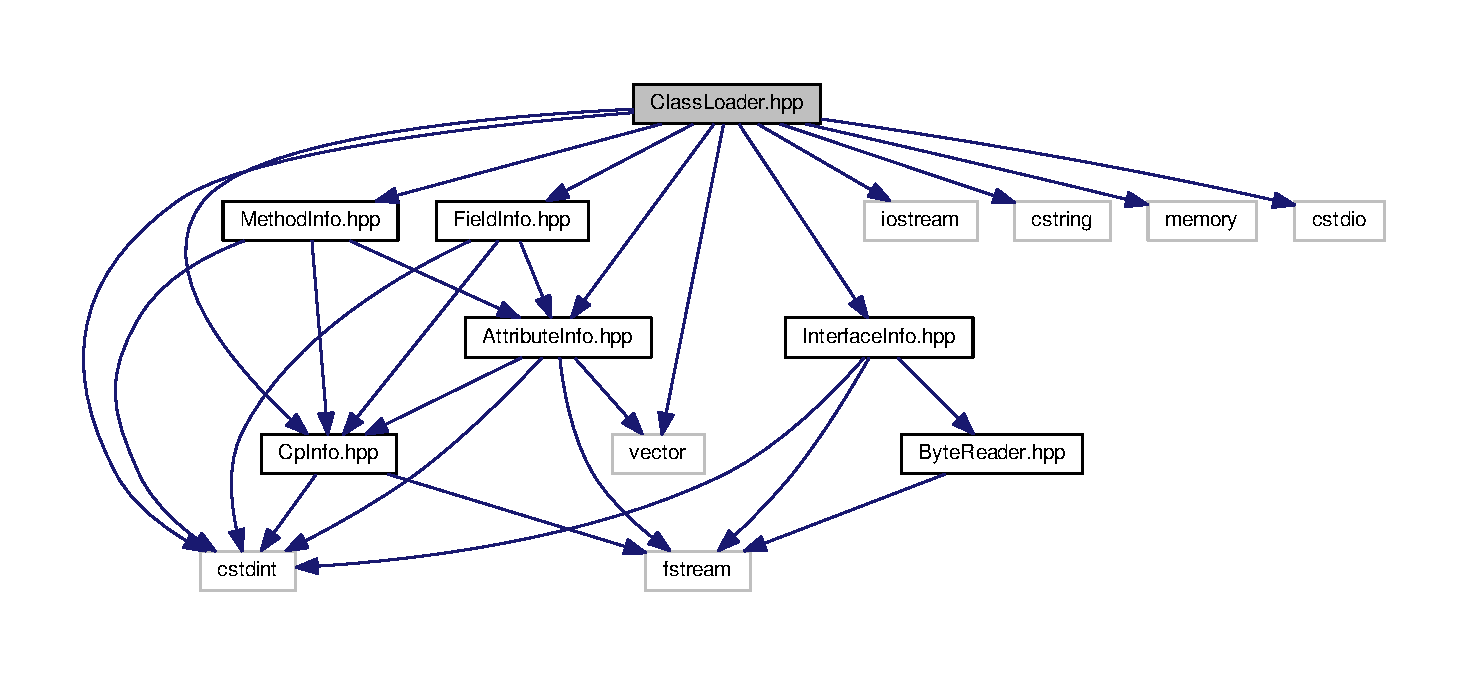
\includegraphics[width=350pt]{_class_loader_8hpp__incl}
\end{center}
\end{figure}
Este grafo mostra quais são os ficheiros que incluem directamente ou indirectamente este ficheiro\+:
\nopagebreak
\begin{figure}[H]
\begin{center}
\leavevmode
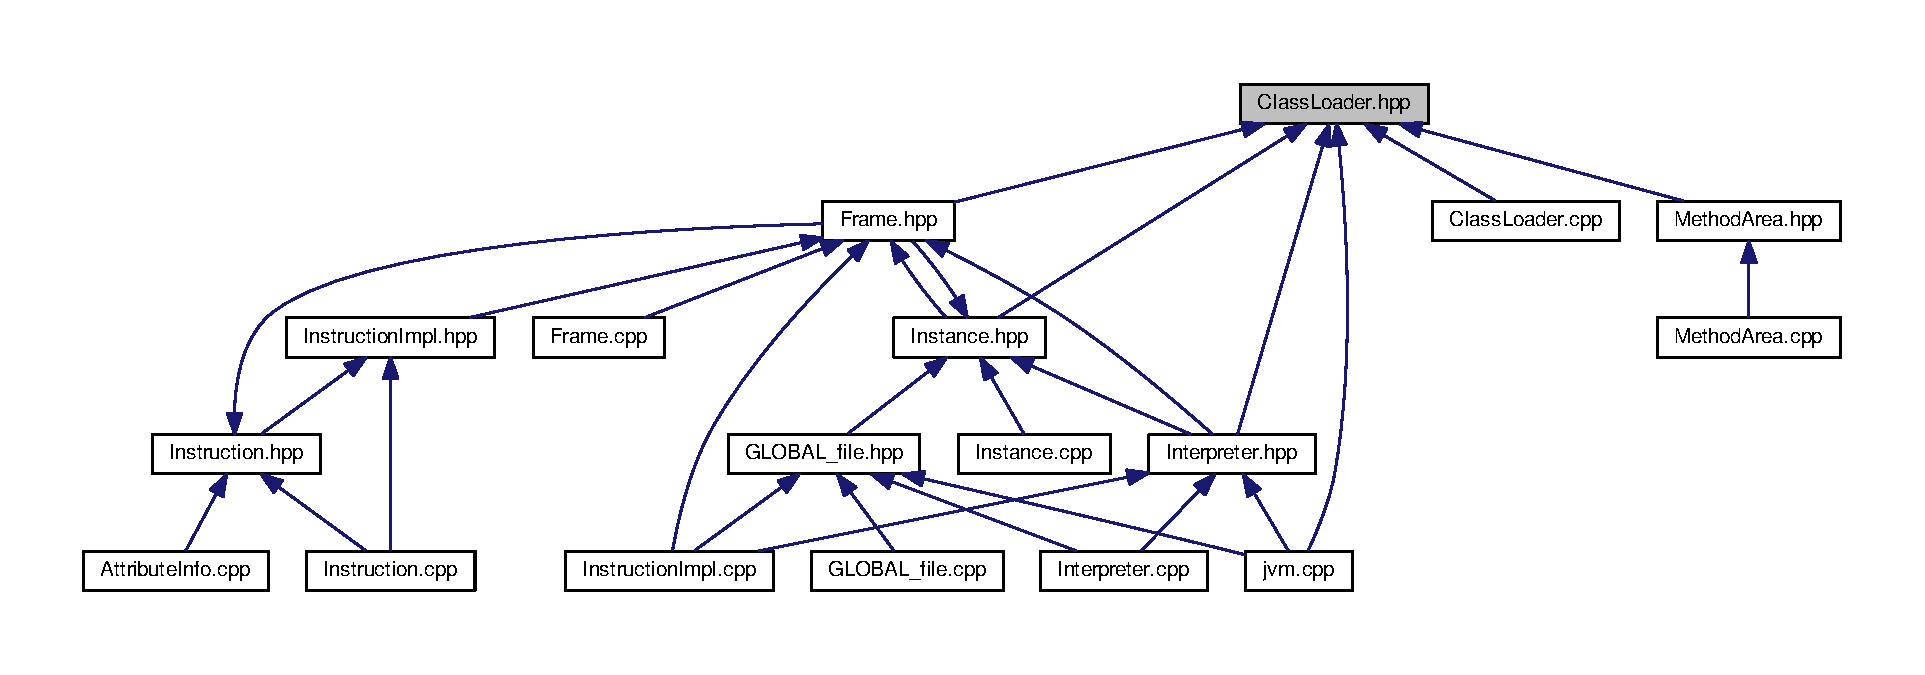
\includegraphics[width=350pt]{_class_loader_8hpp__dep__incl}
\end{center}
\end{figure}
\subsection*{Componentes}
\begin{DoxyCompactItemize}
\item 
class \hyperlink{class_class_loader}{Class\+Loader}
\begin{DoxyCompactList}\small\item\em Todo funcionamento do class\+Loader em relação ao local de armazenamento enquanto é feito a leitura, separando de acordo com que for chamado os metodos de set e get; Além disso, contém destructor;. \end{DoxyCompactList}\end{DoxyCompactItemize}
\subsection*{Macros}
\begin{DoxyCompactItemize}
\item 
\#define \hyperlink{_class_loader_8hpp_a54061e5993a5517320d425f44408cc86}{M\+A\+G\+I\+C\+\_\+\+N\+U\+M\+B\+ER}~0x\+C\+A\+F\+E\+B\+A\+B\+E;
\item 
\#define \hyperlink{_class_loader_8hpp_afc46559a7d3f7baf519fc183c2fad2b4}{C\+O\+N\+S\+T\+A\+N\+T\+\_\+\+Utf8}~1
\item 
\#define \hyperlink{_class_loader_8hpp_a856a6553a55d721970ca5450eb1ccd2c}{C\+O\+N\+S\+T\+A\+N\+T\+\_\+\+Integer}~3
\item 
\#define \hyperlink{_class_loader_8hpp_ab914627ce5b25c4acfc98f2eacb78473}{C\+O\+N\+S\+T\+A\+N\+T\+\_\+\+Float}~4
\item 
\#define \hyperlink{_class_loader_8hpp_a426ca017b895fc522671a561d460be7a}{C\+O\+N\+S\+T\+A\+N\+T\+\_\+\+Long}~5
\item 
\#define \hyperlink{_class_loader_8hpp_ab49341c3b4ade4bfa1a64be8d2f73ae1}{C\+O\+N\+S\+T\+A\+N\+T\+\_\+\+Double}~6
\item 
\#define \hyperlink{_class_loader_8hpp_a72b5b534aa409975da610a36f648fa0a}{C\+O\+N\+S\+T\+A\+N\+T\+\_\+\+Class}~7
\item 
\#define \hyperlink{_class_loader_8hpp_a0a7acbe175de56072a2f0a1a051418e1}{C\+O\+N\+S\+T\+A\+N\+T\+\_\+\+String}~8
\item 
\#define \hyperlink{_class_loader_8hpp_a008d43478c2e2973e7413f5d1c48095d}{C\+O\+N\+S\+T\+A\+N\+T\+\_\+\+Fieldref}~9
\item 
\#define \hyperlink{_class_loader_8hpp_a2a179cf178ea867c6ab1700508c269dd}{C\+O\+N\+S\+T\+A\+N\+T\+\_\+\+Methodref}~10
\item 
\#define \hyperlink{_class_loader_8hpp_ac0e92044d246c6e4d691116f89a70ebb}{C\+O\+N\+S\+T\+A\+N\+T\+\_\+\+Interface\+Methodref}~11
\item 
\#define \hyperlink{_class_loader_8hpp_a5b6ba749976ae61415983ca0b890c91a}{C\+O\+N\+S\+T\+A\+N\+T\+\_\+\+Name\+And\+Type}~12
\item 
\#define \hyperlink{_class_loader_8hpp_ab85a3d64bf30a684b04ebcfcad50f7a0}{C\+O\+N\+S\+T\+A\+N\+T\+\_\+\+Boolean}~90
\item 
\#define \hyperlink{_class_loader_8hpp_ad9a1ec0b184ffdb5591f7bb4e960c58e}{C\+O\+N\+S\+T\+A\+N\+T\+\_\+\+Byte}~91
\item 
\#define \hyperlink{_class_loader_8hpp_a9c59bcd88e83b3d6a9411abcd33cb767}{C\+O\+N\+S\+T\+A\+N\+T\+\_\+\+Char}~92
\item 
\#define \hyperlink{_class_loader_8hpp_a3fbf89e8d1ed392297ffa934eb4d5446}{C\+O\+N\+S\+T\+A\+N\+T\+\_\+\+Short}~93
\item 
\#define \hyperlink{_class_loader_8hpp_ad6c4fa0eab0f32e07df19a02ade24c10}{C\+O\+N\+S\+T\+A\+N\+T\+\_\+\+Array}~94
\item 
\#define \hyperlink{_class_loader_8hpp_a2918a974a2846135428f3b632706416d}{C\+O\+N\+S\+T\+A\+N\+T\+\_\+\+Empty}~0
\item 
\#define \hyperlink{_class_loader_8hpp_a1119e6ec77bb1767207342f9748fd6cf}{typeof}~\+\_\+\+\_\+typeof\+\_\+\+\_\+
\end{DoxyCompactItemize}


\subsection{Descrição detalhada}
Declarações das funções do \hyperlink{class_class_loader}{Class\+Loader} para salvar todos os bytes de .class corretamente. 

\begin{DoxyRefDesc}{Bug}
\item[\hyperlink{bug__bug000003}{Bug}]No known bugs. \end{DoxyRefDesc}


\subsection{Documentação das macros}
\index{Class\+Loader.\+hpp@{Class\+Loader.\+hpp}!C\+O\+N\+S\+T\+A\+N\+T\+\_\+\+Array@{C\+O\+N\+S\+T\+A\+N\+T\+\_\+\+Array}}
\index{C\+O\+N\+S\+T\+A\+N\+T\+\_\+\+Array@{C\+O\+N\+S\+T\+A\+N\+T\+\_\+\+Array}!Class\+Loader.\+hpp@{Class\+Loader.\+hpp}}
\subsubsection[{\texorpdfstring{C\+O\+N\+S\+T\+A\+N\+T\+\_\+\+Array}{CONSTANT_Array}}]{\setlength{\rightskip}{0pt plus 5cm}\#define C\+O\+N\+S\+T\+A\+N\+T\+\_\+\+Array~94}\hypertarget{_class_loader_8hpp_ad6c4fa0eab0f32e07df19a02ade24c10}{}\label{_class_loader_8hpp_ad6c4fa0eab0f32e07df19a02ade24c10}
\index{Class\+Loader.\+hpp@{Class\+Loader.\+hpp}!C\+O\+N\+S\+T\+A\+N\+T\+\_\+\+Boolean@{C\+O\+N\+S\+T\+A\+N\+T\+\_\+\+Boolean}}
\index{C\+O\+N\+S\+T\+A\+N\+T\+\_\+\+Boolean@{C\+O\+N\+S\+T\+A\+N\+T\+\_\+\+Boolean}!Class\+Loader.\+hpp@{Class\+Loader.\+hpp}}
\subsubsection[{\texorpdfstring{C\+O\+N\+S\+T\+A\+N\+T\+\_\+\+Boolean}{CONSTANT_Boolean}}]{\setlength{\rightskip}{0pt plus 5cm}\#define C\+O\+N\+S\+T\+A\+N\+T\+\_\+\+Boolean~90}\hypertarget{_class_loader_8hpp_ab85a3d64bf30a684b04ebcfcad50f7a0}{}\label{_class_loader_8hpp_ab85a3d64bf30a684b04ebcfcad50f7a0}
\index{Class\+Loader.\+hpp@{Class\+Loader.\+hpp}!C\+O\+N\+S\+T\+A\+N\+T\+\_\+\+Byte@{C\+O\+N\+S\+T\+A\+N\+T\+\_\+\+Byte}}
\index{C\+O\+N\+S\+T\+A\+N\+T\+\_\+\+Byte@{C\+O\+N\+S\+T\+A\+N\+T\+\_\+\+Byte}!Class\+Loader.\+hpp@{Class\+Loader.\+hpp}}
\subsubsection[{\texorpdfstring{C\+O\+N\+S\+T\+A\+N\+T\+\_\+\+Byte}{CONSTANT_Byte}}]{\setlength{\rightskip}{0pt plus 5cm}\#define C\+O\+N\+S\+T\+A\+N\+T\+\_\+\+Byte~91}\hypertarget{_class_loader_8hpp_ad9a1ec0b184ffdb5591f7bb4e960c58e}{}\label{_class_loader_8hpp_ad9a1ec0b184ffdb5591f7bb4e960c58e}
\index{Class\+Loader.\+hpp@{Class\+Loader.\+hpp}!C\+O\+N\+S\+T\+A\+N\+T\+\_\+\+Char@{C\+O\+N\+S\+T\+A\+N\+T\+\_\+\+Char}}
\index{C\+O\+N\+S\+T\+A\+N\+T\+\_\+\+Char@{C\+O\+N\+S\+T\+A\+N\+T\+\_\+\+Char}!Class\+Loader.\+hpp@{Class\+Loader.\+hpp}}
\subsubsection[{\texorpdfstring{C\+O\+N\+S\+T\+A\+N\+T\+\_\+\+Char}{CONSTANT_Char}}]{\setlength{\rightskip}{0pt plus 5cm}\#define C\+O\+N\+S\+T\+A\+N\+T\+\_\+\+Char~92}\hypertarget{_class_loader_8hpp_a9c59bcd88e83b3d6a9411abcd33cb767}{}\label{_class_loader_8hpp_a9c59bcd88e83b3d6a9411abcd33cb767}
\index{Class\+Loader.\+hpp@{Class\+Loader.\+hpp}!C\+O\+N\+S\+T\+A\+N\+T\+\_\+\+Class@{C\+O\+N\+S\+T\+A\+N\+T\+\_\+\+Class}}
\index{C\+O\+N\+S\+T\+A\+N\+T\+\_\+\+Class@{C\+O\+N\+S\+T\+A\+N\+T\+\_\+\+Class}!Class\+Loader.\+hpp@{Class\+Loader.\+hpp}}
\subsubsection[{\texorpdfstring{C\+O\+N\+S\+T\+A\+N\+T\+\_\+\+Class}{CONSTANT_Class}}]{\setlength{\rightskip}{0pt plus 5cm}\#define C\+O\+N\+S\+T\+A\+N\+T\+\_\+\+Class~7}\hypertarget{_class_loader_8hpp_a72b5b534aa409975da610a36f648fa0a}{}\label{_class_loader_8hpp_a72b5b534aa409975da610a36f648fa0a}
\index{Class\+Loader.\+hpp@{Class\+Loader.\+hpp}!C\+O\+N\+S\+T\+A\+N\+T\+\_\+\+Double@{C\+O\+N\+S\+T\+A\+N\+T\+\_\+\+Double}}
\index{C\+O\+N\+S\+T\+A\+N\+T\+\_\+\+Double@{C\+O\+N\+S\+T\+A\+N\+T\+\_\+\+Double}!Class\+Loader.\+hpp@{Class\+Loader.\+hpp}}
\subsubsection[{\texorpdfstring{C\+O\+N\+S\+T\+A\+N\+T\+\_\+\+Double}{CONSTANT_Double}}]{\setlength{\rightskip}{0pt plus 5cm}\#define C\+O\+N\+S\+T\+A\+N\+T\+\_\+\+Double~6}\hypertarget{_class_loader_8hpp_ab49341c3b4ade4bfa1a64be8d2f73ae1}{}\label{_class_loader_8hpp_ab49341c3b4ade4bfa1a64be8d2f73ae1}
\index{Class\+Loader.\+hpp@{Class\+Loader.\+hpp}!C\+O\+N\+S\+T\+A\+N\+T\+\_\+\+Empty@{C\+O\+N\+S\+T\+A\+N\+T\+\_\+\+Empty}}
\index{C\+O\+N\+S\+T\+A\+N\+T\+\_\+\+Empty@{C\+O\+N\+S\+T\+A\+N\+T\+\_\+\+Empty}!Class\+Loader.\+hpp@{Class\+Loader.\+hpp}}
\subsubsection[{\texorpdfstring{C\+O\+N\+S\+T\+A\+N\+T\+\_\+\+Empty}{CONSTANT_Empty}}]{\setlength{\rightskip}{0pt plus 5cm}\#define C\+O\+N\+S\+T\+A\+N\+T\+\_\+\+Empty~0}\hypertarget{_class_loader_8hpp_a2918a974a2846135428f3b632706416d}{}\label{_class_loader_8hpp_a2918a974a2846135428f3b632706416d}
\index{Class\+Loader.\+hpp@{Class\+Loader.\+hpp}!C\+O\+N\+S\+T\+A\+N\+T\+\_\+\+Fieldref@{C\+O\+N\+S\+T\+A\+N\+T\+\_\+\+Fieldref}}
\index{C\+O\+N\+S\+T\+A\+N\+T\+\_\+\+Fieldref@{C\+O\+N\+S\+T\+A\+N\+T\+\_\+\+Fieldref}!Class\+Loader.\+hpp@{Class\+Loader.\+hpp}}
\subsubsection[{\texorpdfstring{C\+O\+N\+S\+T\+A\+N\+T\+\_\+\+Fieldref}{CONSTANT_Fieldref}}]{\setlength{\rightskip}{0pt plus 5cm}\#define C\+O\+N\+S\+T\+A\+N\+T\+\_\+\+Fieldref~9}\hypertarget{_class_loader_8hpp_a008d43478c2e2973e7413f5d1c48095d}{}\label{_class_loader_8hpp_a008d43478c2e2973e7413f5d1c48095d}
\index{Class\+Loader.\+hpp@{Class\+Loader.\+hpp}!C\+O\+N\+S\+T\+A\+N\+T\+\_\+\+Float@{C\+O\+N\+S\+T\+A\+N\+T\+\_\+\+Float}}
\index{C\+O\+N\+S\+T\+A\+N\+T\+\_\+\+Float@{C\+O\+N\+S\+T\+A\+N\+T\+\_\+\+Float}!Class\+Loader.\+hpp@{Class\+Loader.\+hpp}}
\subsubsection[{\texorpdfstring{C\+O\+N\+S\+T\+A\+N\+T\+\_\+\+Float}{CONSTANT_Float}}]{\setlength{\rightskip}{0pt plus 5cm}\#define C\+O\+N\+S\+T\+A\+N\+T\+\_\+\+Float~4}\hypertarget{_class_loader_8hpp_ab914627ce5b25c4acfc98f2eacb78473}{}\label{_class_loader_8hpp_ab914627ce5b25c4acfc98f2eacb78473}
\index{Class\+Loader.\+hpp@{Class\+Loader.\+hpp}!C\+O\+N\+S\+T\+A\+N\+T\+\_\+\+Integer@{C\+O\+N\+S\+T\+A\+N\+T\+\_\+\+Integer}}
\index{C\+O\+N\+S\+T\+A\+N\+T\+\_\+\+Integer@{C\+O\+N\+S\+T\+A\+N\+T\+\_\+\+Integer}!Class\+Loader.\+hpp@{Class\+Loader.\+hpp}}
\subsubsection[{\texorpdfstring{C\+O\+N\+S\+T\+A\+N\+T\+\_\+\+Integer}{CONSTANT_Integer}}]{\setlength{\rightskip}{0pt plus 5cm}\#define C\+O\+N\+S\+T\+A\+N\+T\+\_\+\+Integer~3}\hypertarget{_class_loader_8hpp_a856a6553a55d721970ca5450eb1ccd2c}{}\label{_class_loader_8hpp_a856a6553a55d721970ca5450eb1ccd2c}
\index{Class\+Loader.\+hpp@{Class\+Loader.\+hpp}!C\+O\+N\+S\+T\+A\+N\+T\+\_\+\+Interface\+Methodref@{C\+O\+N\+S\+T\+A\+N\+T\+\_\+\+Interface\+Methodref}}
\index{C\+O\+N\+S\+T\+A\+N\+T\+\_\+\+Interface\+Methodref@{C\+O\+N\+S\+T\+A\+N\+T\+\_\+\+Interface\+Methodref}!Class\+Loader.\+hpp@{Class\+Loader.\+hpp}}
\subsubsection[{\texorpdfstring{C\+O\+N\+S\+T\+A\+N\+T\+\_\+\+Interface\+Methodref}{CONSTANT_InterfaceMethodref}}]{\setlength{\rightskip}{0pt plus 5cm}\#define C\+O\+N\+S\+T\+A\+N\+T\+\_\+\+Interface\+Methodref~11}\hypertarget{_class_loader_8hpp_ac0e92044d246c6e4d691116f89a70ebb}{}\label{_class_loader_8hpp_ac0e92044d246c6e4d691116f89a70ebb}
\index{Class\+Loader.\+hpp@{Class\+Loader.\+hpp}!C\+O\+N\+S\+T\+A\+N\+T\+\_\+\+Long@{C\+O\+N\+S\+T\+A\+N\+T\+\_\+\+Long}}
\index{C\+O\+N\+S\+T\+A\+N\+T\+\_\+\+Long@{C\+O\+N\+S\+T\+A\+N\+T\+\_\+\+Long}!Class\+Loader.\+hpp@{Class\+Loader.\+hpp}}
\subsubsection[{\texorpdfstring{C\+O\+N\+S\+T\+A\+N\+T\+\_\+\+Long}{CONSTANT_Long}}]{\setlength{\rightskip}{0pt plus 5cm}\#define C\+O\+N\+S\+T\+A\+N\+T\+\_\+\+Long~5}\hypertarget{_class_loader_8hpp_a426ca017b895fc522671a561d460be7a}{}\label{_class_loader_8hpp_a426ca017b895fc522671a561d460be7a}
\index{Class\+Loader.\+hpp@{Class\+Loader.\+hpp}!C\+O\+N\+S\+T\+A\+N\+T\+\_\+\+Methodref@{C\+O\+N\+S\+T\+A\+N\+T\+\_\+\+Methodref}}
\index{C\+O\+N\+S\+T\+A\+N\+T\+\_\+\+Methodref@{C\+O\+N\+S\+T\+A\+N\+T\+\_\+\+Methodref}!Class\+Loader.\+hpp@{Class\+Loader.\+hpp}}
\subsubsection[{\texorpdfstring{C\+O\+N\+S\+T\+A\+N\+T\+\_\+\+Methodref}{CONSTANT_Methodref}}]{\setlength{\rightskip}{0pt plus 5cm}\#define C\+O\+N\+S\+T\+A\+N\+T\+\_\+\+Methodref~10}\hypertarget{_class_loader_8hpp_a2a179cf178ea867c6ab1700508c269dd}{}\label{_class_loader_8hpp_a2a179cf178ea867c6ab1700508c269dd}
\index{Class\+Loader.\+hpp@{Class\+Loader.\+hpp}!C\+O\+N\+S\+T\+A\+N\+T\+\_\+\+Name\+And\+Type@{C\+O\+N\+S\+T\+A\+N\+T\+\_\+\+Name\+And\+Type}}
\index{C\+O\+N\+S\+T\+A\+N\+T\+\_\+\+Name\+And\+Type@{C\+O\+N\+S\+T\+A\+N\+T\+\_\+\+Name\+And\+Type}!Class\+Loader.\+hpp@{Class\+Loader.\+hpp}}
\subsubsection[{\texorpdfstring{C\+O\+N\+S\+T\+A\+N\+T\+\_\+\+Name\+And\+Type}{CONSTANT_NameAndType}}]{\setlength{\rightskip}{0pt plus 5cm}\#define C\+O\+N\+S\+T\+A\+N\+T\+\_\+\+Name\+And\+Type~12}\hypertarget{_class_loader_8hpp_a5b6ba749976ae61415983ca0b890c91a}{}\label{_class_loader_8hpp_a5b6ba749976ae61415983ca0b890c91a}
\index{Class\+Loader.\+hpp@{Class\+Loader.\+hpp}!C\+O\+N\+S\+T\+A\+N\+T\+\_\+\+Short@{C\+O\+N\+S\+T\+A\+N\+T\+\_\+\+Short}}
\index{C\+O\+N\+S\+T\+A\+N\+T\+\_\+\+Short@{C\+O\+N\+S\+T\+A\+N\+T\+\_\+\+Short}!Class\+Loader.\+hpp@{Class\+Loader.\+hpp}}
\subsubsection[{\texorpdfstring{C\+O\+N\+S\+T\+A\+N\+T\+\_\+\+Short}{CONSTANT_Short}}]{\setlength{\rightskip}{0pt plus 5cm}\#define C\+O\+N\+S\+T\+A\+N\+T\+\_\+\+Short~93}\hypertarget{_class_loader_8hpp_a3fbf89e8d1ed392297ffa934eb4d5446}{}\label{_class_loader_8hpp_a3fbf89e8d1ed392297ffa934eb4d5446}
\index{Class\+Loader.\+hpp@{Class\+Loader.\+hpp}!C\+O\+N\+S\+T\+A\+N\+T\+\_\+\+String@{C\+O\+N\+S\+T\+A\+N\+T\+\_\+\+String}}
\index{C\+O\+N\+S\+T\+A\+N\+T\+\_\+\+String@{C\+O\+N\+S\+T\+A\+N\+T\+\_\+\+String}!Class\+Loader.\+hpp@{Class\+Loader.\+hpp}}
\subsubsection[{\texorpdfstring{C\+O\+N\+S\+T\+A\+N\+T\+\_\+\+String}{CONSTANT_String}}]{\setlength{\rightskip}{0pt plus 5cm}\#define C\+O\+N\+S\+T\+A\+N\+T\+\_\+\+String~8}\hypertarget{_class_loader_8hpp_a0a7acbe175de56072a2f0a1a051418e1}{}\label{_class_loader_8hpp_a0a7acbe175de56072a2f0a1a051418e1}
\index{Class\+Loader.\+hpp@{Class\+Loader.\+hpp}!C\+O\+N\+S\+T\+A\+N\+T\+\_\+\+Utf8@{C\+O\+N\+S\+T\+A\+N\+T\+\_\+\+Utf8}}
\index{C\+O\+N\+S\+T\+A\+N\+T\+\_\+\+Utf8@{C\+O\+N\+S\+T\+A\+N\+T\+\_\+\+Utf8}!Class\+Loader.\+hpp@{Class\+Loader.\+hpp}}
\subsubsection[{\texorpdfstring{C\+O\+N\+S\+T\+A\+N\+T\+\_\+\+Utf8}{CONSTANT_Utf8}}]{\setlength{\rightskip}{0pt plus 5cm}\#define C\+O\+N\+S\+T\+A\+N\+T\+\_\+\+Utf8~1}\hypertarget{_class_loader_8hpp_afc46559a7d3f7baf519fc183c2fad2b4}{}\label{_class_loader_8hpp_afc46559a7d3f7baf519fc183c2fad2b4}
\index{Class\+Loader.\+hpp@{Class\+Loader.\+hpp}!M\+A\+G\+I\+C\+\_\+\+N\+U\+M\+B\+ER@{M\+A\+G\+I\+C\+\_\+\+N\+U\+M\+B\+ER}}
\index{M\+A\+G\+I\+C\+\_\+\+N\+U\+M\+B\+ER@{M\+A\+G\+I\+C\+\_\+\+N\+U\+M\+B\+ER}!Class\+Loader.\+hpp@{Class\+Loader.\+hpp}}
\subsubsection[{\texorpdfstring{M\+A\+G\+I\+C\+\_\+\+N\+U\+M\+B\+ER}{MAGIC_NUMBER}}]{\setlength{\rightskip}{0pt plus 5cm}\#define M\+A\+G\+I\+C\+\_\+\+N\+U\+M\+B\+ER~0x\+C\+A\+F\+E\+B\+A\+B\+E;}\hypertarget{_class_loader_8hpp_a54061e5993a5517320d425f44408cc86}{}\label{_class_loader_8hpp_a54061e5993a5517320d425f44408cc86}
\index{Class\+Loader.\+hpp@{Class\+Loader.\+hpp}!typeof@{typeof}}
\index{typeof@{typeof}!Class\+Loader.\+hpp@{Class\+Loader.\+hpp}}
\subsubsection[{\texorpdfstring{typeof}{typeof}}]{\setlength{\rightskip}{0pt plus 5cm}\#define typeof~\+\_\+\+\_\+typeof\+\_\+\+\_\+}\hypertarget{_class_loader_8hpp_a1119e6ec77bb1767207342f9748fd6cf}{}\label{_class_loader_8hpp_a1119e6ec77bb1767207342f9748fd6cf}

\hypertarget{_cp_attribute_interface_8cpp}{}\section{Referência ao ficheiro Cp\+Attribute\+Interface.\+cpp}
\label{_cp_attribute_interface_8cpp}\index{Cp\+Attribute\+Interface.\+cpp@{Cp\+Attribute\+Interface.\+cpp}}


Funções que verificam, a partir da tag, qual o tipo do bytecode que está sendo lido;.  


{\ttfamily \#include \char`\"{}Cp\+Attribute\+Interface.\+hpp\char`\"{}}\\*
Diagrama de dependências de inclusão para Cp\+Attribute\+Interface.\+cpp\+:
\nopagebreak
\begin{figure}[H]
\begin{center}
\leavevmode
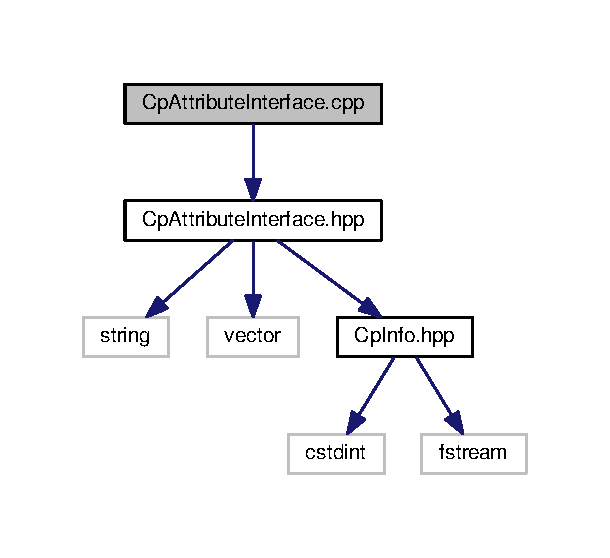
\includegraphics[width=293pt]{_cp_attribute_interface_8cpp__incl}
\end{center}
\end{figure}
\subsection*{Macros}
\begin{DoxyCompactItemize}
\item 
\#define \hyperlink{_cp_attribute_interface_8cpp_afc46559a7d3f7baf519fc183c2fad2b4}{C\+O\+N\+S\+T\+A\+N\+T\+\_\+\+Utf8}~1
\item 
\#define \hyperlink{_cp_attribute_interface_8cpp_a856a6553a55d721970ca5450eb1ccd2c}{C\+O\+N\+S\+T\+A\+N\+T\+\_\+\+Integer}~3
\item 
\#define \hyperlink{_cp_attribute_interface_8cpp_ab914627ce5b25c4acfc98f2eacb78473}{C\+O\+N\+S\+T\+A\+N\+T\+\_\+\+Float}~4
\item 
\#define \hyperlink{_cp_attribute_interface_8cpp_a426ca017b895fc522671a561d460be7a}{C\+O\+N\+S\+T\+A\+N\+T\+\_\+\+Long}~5
\item 
\#define \hyperlink{_cp_attribute_interface_8cpp_ab49341c3b4ade4bfa1a64be8d2f73ae1}{C\+O\+N\+S\+T\+A\+N\+T\+\_\+\+Double}~6
\item 
\#define \hyperlink{_cp_attribute_interface_8cpp_a72b5b534aa409975da610a36f648fa0a}{C\+O\+N\+S\+T\+A\+N\+T\+\_\+\+Class}~7
\item 
\#define \hyperlink{_cp_attribute_interface_8cpp_a0a7acbe175de56072a2f0a1a051418e1}{C\+O\+N\+S\+T\+A\+N\+T\+\_\+\+String}~8
\item 
\#define \hyperlink{_cp_attribute_interface_8cpp_a008d43478c2e2973e7413f5d1c48095d}{C\+O\+N\+S\+T\+A\+N\+T\+\_\+\+Fieldref}~9
\item 
\#define \hyperlink{_cp_attribute_interface_8cpp_a2a179cf178ea867c6ab1700508c269dd}{C\+O\+N\+S\+T\+A\+N\+T\+\_\+\+Methodref}~10
\item 
\#define \hyperlink{_cp_attribute_interface_8cpp_ac0e92044d246c6e4d691116f89a70ebb}{C\+O\+N\+S\+T\+A\+N\+T\+\_\+\+Interface\+Methodref}~11
\item 
\#define \hyperlink{_cp_attribute_interface_8cpp_a5b6ba749976ae61415983ca0b890c91a}{C\+O\+N\+S\+T\+A\+N\+T\+\_\+\+Name\+And\+Type}~12
\item 
\#define \hyperlink{_cp_attribute_interface_8cpp_a2918a974a2846135428f3b632706416d}{C\+O\+N\+S\+T\+A\+N\+T\+\_\+\+Empty}~0
\end{DoxyCompactItemize}


\subsection{Descrição detalhada}
Funções que verificam, a partir da tag, qual o tipo do bytecode que está sendo lido;. 



\subsection{Documentação das macros}
\index{Cp\+Attribute\+Interface.\+cpp@{Cp\+Attribute\+Interface.\+cpp}!C\+O\+N\+S\+T\+A\+N\+T\+\_\+\+Class@{C\+O\+N\+S\+T\+A\+N\+T\+\_\+\+Class}}
\index{C\+O\+N\+S\+T\+A\+N\+T\+\_\+\+Class@{C\+O\+N\+S\+T\+A\+N\+T\+\_\+\+Class}!Cp\+Attribute\+Interface.\+cpp@{Cp\+Attribute\+Interface.\+cpp}}
\subsubsection[{\texorpdfstring{C\+O\+N\+S\+T\+A\+N\+T\+\_\+\+Class}{CONSTANT_Class}}]{\setlength{\rightskip}{0pt plus 5cm}\#define C\+O\+N\+S\+T\+A\+N\+T\+\_\+\+Class~7}\hypertarget{_cp_attribute_interface_8cpp_a72b5b534aa409975da610a36f648fa0a}{}\label{_cp_attribute_interface_8cpp_a72b5b534aa409975da610a36f648fa0a}
\index{Cp\+Attribute\+Interface.\+cpp@{Cp\+Attribute\+Interface.\+cpp}!C\+O\+N\+S\+T\+A\+N\+T\+\_\+\+Double@{C\+O\+N\+S\+T\+A\+N\+T\+\_\+\+Double}}
\index{C\+O\+N\+S\+T\+A\+N\+T\+\_\+\+Double@{C\+O\+N\+S\+T\+A\+N\+T\+\_\+\+Double}!Cp\+Attribute\+Interface.\+cpp@{Cp\+Attribute\+Interface.\+cpp}}
\subsubsection[{\texorpdfstring{C\+O\+N\+S\+T\+A\+N\+T\+\_\+\+Double}{CONSTANT_Double}}]{\setlength{\rightskip}{0pt plus 5cm}\#define C\+O\+N\+S\+T\+A\+N\+T\+\_\+\+Double~6}\hypertarget{_cp_attribute_interface_8cpp_ab49341c3b4ade4bfa1a64be8d2f73ae1}{}\label{_cp_attribute_interface_8cpp_ab49341c3b4ade4bfa1a64be8d2f73ae1}
\index{Cp\+Attribute\+Interface.\+cpp@{Cp\+Attribute\+Interface.\+cpp}!C\+O\+N\+S\+T\+A\+N\+T\+\_\+\+Empty@{C\+O\+N\+S\+T\+A\+N\+T\+\_\+\+Empty}}
\index{C\+O\+N\+S\+T\+A\+N\+T\+\_\+\+Empty@{C\+O\+N\+S\+T\+A\+N\+T\+\_\+\+Empty}!Cp\+Attribute\+Interface.\+cpp@{Cp\+Attribute\+Interface.\+cpp}}
\subsubsection[{\texorpdfstring{C\+O\+N\+S\+T\+A\+N\+T\+\_\+\+Empty}{CONSTANT_Empty}}]{\setlength{\rightskip}{0pt plus 5cm}\#define C\+O\+N\+S\+T\+A\+N\+T\+\_\+\+Empty~0}\hypertarget{_cp_attribute_interface_8cpp_a2918a974a2846135428f3b632706416d}{}\label{_cp_attribute_interface_8cpp_a2918a974a2846135428f3b632706416d}
\index{Cp\+Attribute\+Interface.\+cpp@{Cp\+Attribute\+Interface.\+cpp}!C\+O\+N\+S\+T\+A\+N\+T\+\_\+\+Fieldref@{C\+O\+N\+S\+T\+A\+N\+T\+\_\+\+Fieldref}}
\index{C\+O\+N\+S\+T\+A\+N\+T\+\_\+\+Fieldref@{C\+O\+N\+S\+T\+A\+N\+T\+\_\+\+Fieldref}!Cp\+Attribute\+Interface.\+cpp@{Cp\+Attribute\+Interface.\+cpp}}
\subsubsection[{\texorpdfstring{C\+O\+N\+S\+T\+A\+N\+T\+\_\+\+Fieldref}{CONSTANT_Fieldref}}]{\setlength{\rightskip}{0pt plus 5cm}\#define C\+O\+N\+S\+T\+A\+N\+T\+\_\+\+Fieldref~9}\hypertarget{_cp_attribute_interface_8cpp_a008d43478c2e2973e7413f5d1c48095d}{}\label{_cp_attribute_interface_8cpp_a008d43478c2e2973e7413f5d1c48095d}
\index{Cp\+Attribute\+Interface.\+cpp@{Cp\+Attribute\+Interface.\+cpp}!C\+O\+N\+S\+T\+A\+N\+T\+\_\+\+Float@{C\+O\+N\+S\+T\+A\+N\+T\+\_\+\+Float}}
\index{C\+O\+N\+S\+T\+A\+N\+T\+\_\+\+Float@{C\+O\+N\+S\+T\+A\+N\+T\+\_\+\+Float}!Cp\+Attribute\+Interface.\+cpp@{Cp\+Attribute\+Interface.\+cpp}}
\subsubsection[{\texorpdfstring{C\+O\+N\+S\+T\+A\+N\+T\+\_\+\+Float}{CONSTANT_Float}}]{\setlength{\rightskip}{0pt plus 5cm}\#define C\+O\+N\+S\+T\+A\+N\+T\+\_\+\+Float~4}\hypertarget{_cp_attribute_interface_8cpp_ab914627ce5b25c4acfc98f2eacb78473}{}\label{_cp_attribute_interface_8cpp_ab914627ce5b25c4acfc98f2eacb78473}
\index{Cp\+Attribute\+Interface.\+cpp@{Cp\+Attribute\+Interface.\+cpp}!C\+O\+N\+S\+T\+A\+N\+T\+\_\+\+Integer@{C\+O\+N\+S\+T\+A\+N\+T\+\_\+\+Integer}}
\index{C\+O\+N\+S\+T\+A\+N\+T\+\_\+\+Integer@{C\+O\+N\+S\+T\+A\+N\+T\+\_\+\+Integer}!Cp\+Attribute\+Interface.\+cpp@{Cp\+Attribute\+Interface.\+cpp}}
\subsubsection[{\texorpdfstring{C\+O\+N\+S\+T\+A\+N\+T\+\_\+\+Integer}{CONSTANT_Integer}}]{\setlength{\rightskip}{0pt plus 5cm}\#define C\+O\+N\+S\+T\+A\+N\+T\+\_\+\+Integer~3}\hypertarget{_cp_attribute_interface_8cpp_a856a6553a55d721970ca5450eb1ccd2c}{}\label{_cp_attribute_interface_8cpp_a856a6553a55d721970ca5450eb1ccd2c}
\index{Cp\+Attribute\+Interface.\+cpp@{Cp\+Attribute\+Interface.\+cpp}!C\+O\+N\+S\+T\+A\+N\+T\+\_\+\+Interface\+Methodref@{C\+O\+N\+S\+T\+A\+N\+T\+\_\+\+Interface\+Methodref}}
\index{C\+O\+N\+S\+T\+A\+N\+T\+\_\+\+Interface\+Methodref@{C\+O\+N\+S\+T\+A\+N\+T\+\_\+\+Interface\+Methodref}!Cp\+Attribute\+Interface.\+cpp@{Cp\+Attribute\+Interface.\+cpp}}
\subsubsection[{\texorpdfstring{C\+O\+N\+S\+T\+A\+N\+T\+\_\+\+Interface\+Methodref}{CONSTANT_InterfaceMethodref}}]{\setlength{\rightskip}{0pt plus 5cm}\#define C\+O\+N\+S\+T\+A\+N\+T\+\_\+\+Interface\+Methodref~11}\hypertarget{_cp_attribute_interface_8cpp_ac0e92044d246c6e4d691116f89a70ebb}{}\label{_cp_attribute_interface_8cpp_ac0e92044d246c6e4d691116f89a70ebb}
\index{Cp\+Attribute\+Interface.\+cpp@{Cp\+Attribute\+Interface.\+cpp}!C\+O\+N\+S\+T\+A\+N\+T\+\_\+\+Long@{C\+O\+N\+S\+T\+A\+N\+T\+\_\+\+Long}}
\index{C\+O\+N\+S\+T\+A\+N\+T\+\_\+\+Long@{C\+O\+N\+S\+T\+A\+N\+T\+\_\+\+Long}!Cp\+Attribute\+Interface.\+cpp@{Cp\+Attribute\+Interface.\+cpp}}
\subsubsection[{\texorpdfstring{C\+O\+N\+S\+T\+A\+N\+T\+\_\+\+Long}{CONSTANT_Long}}]{\setlength{\rightskip}{0pt plus 5cm}\#define C\+O\+N\+S\+T\+A\+N\+T\+\_\+\+Long~5}\hypertarget{_cp_attribute_interface_8cpp_a426ca017b895fc522671a561d460be7a}{}\label{_cp_attribute_interface_8cpp_a426ca017b895fc522671a561d460be7a}
\index{Cp\+Attribute\+Interface.\+cpp@{Cp\+Attribute\+Interface.\+cpp}!C\+O\+N\+S\+T\+A\+N\+T\+\_\+\+Methodref@{C\+O\+N\+S\+T\+A\+N\+T\+\_\+\+Methodref}}
\index{C\+O\+N\+S\+T\+A\+N\+T\+\_\+\+Methodref@{C\+O\+N\+S\+T\+A\+N\+T\+\_\+\+Methodref}!Cp\+Attribute\+Interface.\+cpp@{Cp\+Attribute\+Interface.\+cpp}}
\subsubsection[{\texorpdfstring{C\+O\+N\+S\+T\+A\+N\+T\+\_\+\+Methodref}{CONSTANT_Methodref}}]{\setlength{\rightskip}{0pt plus 5cm}\#define C\+O\+N\+S\+T\+A\+N\+T\+\_\+\+Methodref~10}\hypertarget{_cp_attribute_interface_8cpp_a2a179cf178ea867c6ab1700508c269dd}{}\label{_cp_attribute_interface_8cpp_a2a179cf178ea867c6ab1700508c269dd}
\index{Cp\+Attribute\+Interface.\+cpp@{Cp\+Attribute\+Interface.\+cpp}!C\+O\+N\+S\+T\+A\+N\+T\+\_\+\+Name\+And\+Type@{C\+O\+N\+S\+T\+A\+N\+T\+\_\+\+Name\+And\+Type}}
\index{C\+O\+N\+S\+T\+A\+N\+T\+\_\+\+Name\+And\+Type@{C\+O\+N\+S\+T\+A\+N\+T\+\_\+\+Name\+And\+Type}!Cp\+Attribute\+Interface.\+cpp@{Cp\+Attribute\+Interface.\+cpp}}
\subsubsection[{\texorpdfstring{C\+O\+N\+S\+T\+A\+N\+T\+\_\+\+Name\+And\+Type}{CONSTANT_NameAndType}}]{\setlength{\rightskip}{0pt plus 5cm}\#define C\+O\+N\+S\+T\+A\+N\+T\+\_\+\+Name\+And\+Type~12}\hypertarget{_cp_attribute_interface_8cpp_a5b6ba749976ae61415983ca0b890c91a}{}\label{_cp_attribute_interface_8cpp_a5b6ba749976ae61415983ca0b890c91a}
\index{Cp\+Attribute\+Interface.\+cpp@{Cp\+Attribute\+Interface.\+cpp}!C\+O\+N\+S\+T\+A\+N\+T\+\_\+\+String@{C\+O\+N\+S\+T\+A\+N\+T\+\_\+\+String}}
\index{C\+O\+N\+S\+T\+A\+N\+T\+\_\+\+String@{C\+O\+N\+S\+T\+A\+N\+T\+\_\+\+String}!Cp\+Attribute\+Interface.\+cpp@{Cp\+Attribute\+Interface.\+cpp}}
\subsubsection[{\texorpdfstring{C\+O\+N\+S\+T\+A\+N\+T\+\_\+\+String}{CONSTANT_String}}]{\setlength{\rightskip}{0pt plus 5cm}\#define C\+O\+N\+S\+T\+A\+N\+T\+\_\+\+String~8}\hypertarget{_cp_attribute_interface_8cpp_a0a7acbe175de56072a2f0a1a051418e1}{}\label{_cp_attribute_interface_8cpp_a0a7acbe175de56072a2f0a1a051418e1}
\index{Cp\+Attribute\+Interface.\+cpp@{Cp\+Attribute\+Interface.\+cpp}!C\+O\+N\+S\+T\+A\+N\+T\+\_\+\+Utf8@{C\+O\+N\+S\+T\+A\+N\+T\+\_\+\+Utf8}}
\index{C\+O\+N\+S\+T\+A\+N\+T\+\_\+\+Utf8@{C\+O\+N\+S\+T\+A\+N\+T\+\_\+\+Utf8}!Cp\+Attribute\+Interface.\+cpp@{Cp\+Attribute\+Interface.\+cpp}}
\subsubsection[{\texorpdfstring{C\+O\+N\+S\+T\+A\+N\+T\+\_\+\+Utf8}{CONSTANT_Utf8}}]{\setlength{\rightskip}{0pt plus 5cm}\#define C\+O\+N\+S\+T\+A\+N\+T\+\_\+\+Utf8~1}\hypertarget{_cp_attribute_interface_8cpp_afc46559a7d3f7baf519fc183c2fad2b4}{}\label{_cp_attribute_interface_8cpp_afc46559a7d3f7baf519fc183c2fad2b4}

\hypertarget{_cp_attribute_interface_8hpp}{}\section{Referência ao ficheiro Cp\+Attribute\+Interface.\+hpp}
\label{_cp_attribute_interface_8hpp}\index{Cp\+Attribute\+Interface.\+hpp@{Cp\+Attribute\+Interface.\+hpp}}


Declarações da interface entre Constant\+Pool e \hyperlink{class_attribute_info}{Attribute\+Info} para traduzir as strings U\+T\+F8.  


{\ttfamily \#include $<$string$>$}\\*
{\ttfamily \#include $<$vector$>$}\\*
{\ttfamily \#include \char`\"{}Cp\+Info.\+hpp\char`\"{}}\\*
Diagrama de dependências de inclusão para Cp\+Attribute\+Interface.\+hpp\+:
\nopagebreak
\begin{figure}[H]
\begin{center}
\leavevmode
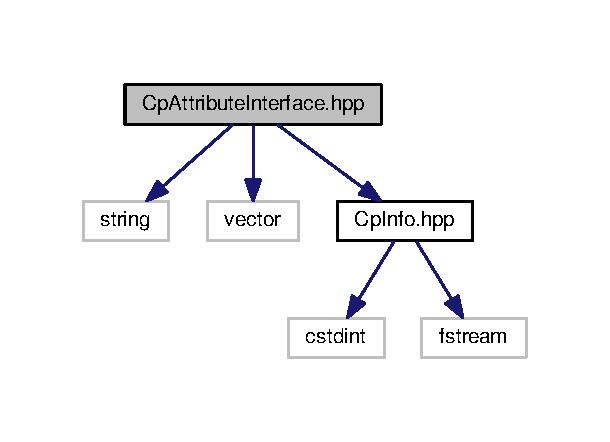
\includegraphics[width=293pt]{_cp_attribute_interface_8hpp__incl}
\end{center}
\end{figure}
Este grafo mostra quais são os ficheiros que incluem directamente ou indirectamente este ficheiro\+:
\nopagebreak
\begin{figure}[H]
\begin{center}
\leavevmode
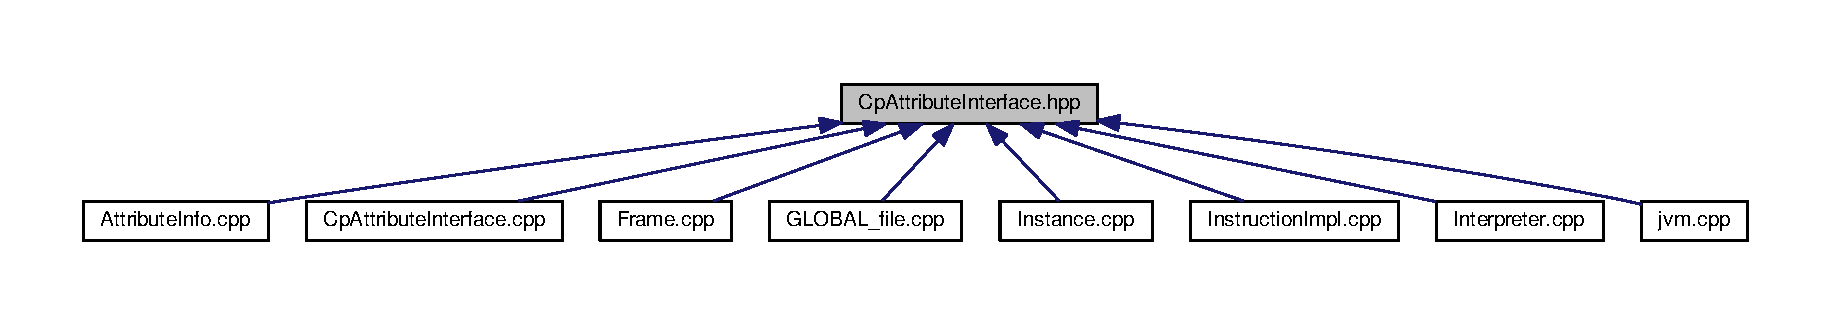
\includegraphics[width=350pt]{_cp_attribute_interface_8hpp__dep__incl}
\end{center}
\end{figure}
\subsection*{Componentes}
\begin{DoxyCompactItemize}
\item 
class \hyperlink{struct_cp_attribute_interface}{Cp\+Attribute\+Interface}
\begin{DoxyCompactList}\small\item\em Declarações da interface entre Constant\+Pool e \hyperlink{class_attribute_info}{Attribute\+Info} para traduzir as strings U\+T\+F8. \end{DoxyCompactList}\end{DoxyCompactItemize}


\subsection{Descrição detalhada}
Declarações da interface entre Constant\+Pool e \hyperlink{class_attribute_info}{Attribute\+Info} para traduzir as strings U\+T\+F8. 

\begin{DoxyRefDesc}{Bug}
\item[\hyperlink{bug__bug000004}{Bug}]No known bugs. \end{DoxyRefDesc}

\hypertarget{_cp_info_8cpp}{}\section{Referência ao ficheiro Cp\+Info.\+cpp}
\label{_cp_info_8cpp}\index{Cp\+Info.\+cpp@{Cp\+Info.\+cpp}}


Ocorre os set\textquotesingle{}s a partir dos bytes lidos no problema;.  


{\ttfamily \#include \char`\"{}Cp\+Info.\+hpp\char`\"{}}\\*
{\ttfamily \#include \char`\"{}Byte\+Reader.\+hpp\char`\"{}}\\*
{\ttfamily \#include $<$iostream$>$}\\*
Diagrama de dependências de inclusão para Cp\+Info.\+cpp\+:
\nopagebreak
\begin{figure}[H]
\begin{center}
\leavevmode
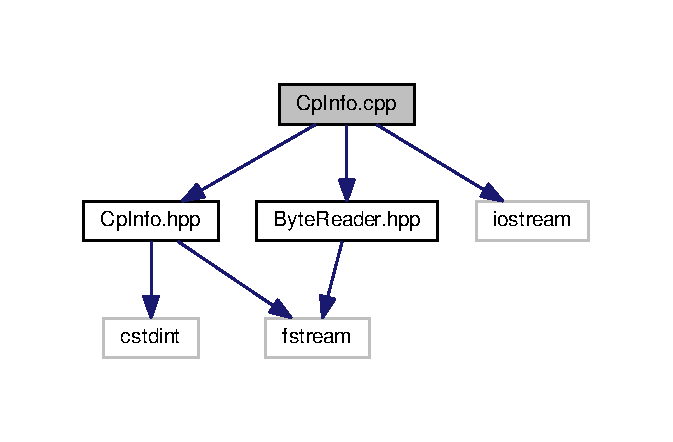
\includegraphics[width=323pt]{_cp_info_8cpp__incl}
\end{center}
\end{figure}
\subsection*{Macros}
\begin{DoxyCompactItemize}
\item 
\#define \hyperlink{_cp_info_8cpp_a5109d53b3b481009c77812a26c4edf33}{C\+P\+P\+\_\+\+C\+P\+I\+N\+FO}
\item 
\#define \hyperlink{_cp_info_8cpp_afc46559a7d3f7baf519fc183c2fad2b4}{C\+O\+N\+S\+T\+A\+N\+T\+\_\+\+Utf8}~1
\item 
\#define \hyperlink{_cp_info_8cpp_a856a6553a55d721970ca5450eb1ccd2c}{C\+O\+N\+S\+T\+A\+N\+T\+\_\+\+Integer}~3
\item 
\#define \hyperlink{_cp_info_8cpp_ab914627ce5b25c4acfc98f2eacb78473}{C\+O\+N\+S\+T\+A\+N\+T\+\_\+\+Float}~4
\item 
\#define \hyperlink{_cp_info_8cpp_a426ca017b895fc522671a561d460be7a}{C\+O\+N\+S\+T\+A\+N\+T\+\_\+\+Long}~5
\item 
\#define \hyperlink{_cp_info_8cpp_ab49341c3b4ade4bfa1a64be8d2f73ae1}{C\+O\+N\+S\+T\+A\+N\+T\+\_\+\+Double}~6
\item 
\#define \hyperlink{_cp_info_8cpp_a72b5b534aa409975da610a36f648fa0a}{C\+O\+N\+S\+T\+A\+N\+T\+\_\+\+Class}~7
\item 
\#define \hyperlink{_cp_info_8cpp_a0a7acbe175de56072a2f0a1a051418e1}{C\+O\+N\+S\+T\+A\+N\+T\+\_\+\+String}~8
\item 
\#define \hyperlink{_cp_info_8cpp_a008d43478c2e2973e7413f5d1c48095d}{C\+O\+N\+S\+T\+A\+N\+T\+\_\+\+Fieldref}~9
\item 
\#define \hyperlink{_cp_info_8cpp_a2a179cf178ea867c6ab1700508c269dd}{C\+O\+N\+S\+T\+A\+N\+T\+\_\+\+Methodref}~10
\item 
\#define \hyperlink{_cp_info_8cpp_ac0e92044d246c6e4d691116f89a70ebb}{C\+O\+N\+S\+T\+A\+N\+T\+\_\+\+Interface\+Methodref}~11
\item 
\#define \hyperlink{_cp_info_8cpp_a5b6ba749976ae61415983ca0b890c91a}{C\+O\+N\+S\+T\+A\+N\+T\+\_\+\+Name\+And\+Type}~12
\item 
\#define \hyperlink{_cp_info_8cpp_a2918a974a2846135428f3b632706416d}{C\+O\+N\+S\+T\+A\+N\+T\+\_\+\+Empty}~0
\end{DoxyCompactItemize}


\subsection{Descrição detalhada}
Ocorre os set\textquotesingle{}s a partir dos bytes lidos no problema;. 



\subsection{Documentação das macros}
\index{Cp\+Info.\+cpp@{Cp\+Info.\+cpp}!C\+O\+N\+S\+T\+A\+N\+T\+\_\+\+Class@{C\+O\+N\+S\+T\+A\+N\+T\+\_\+\+Class}}
\index{C\+O\+N\+S\+T\+A\+N\+T\+\_\+\+Class@{C\+O\+N\+S\+T\+A\+N\+T\+\_\+\+Class}!Cp\+Info.\+cpp@{Cp\+Info.\+cpp}}
\subsubsection[{\texorpdfstring{C\+O\+N\+S\+T\+A\+N\+T\+\_\+\+Class}{CONSTANT_Class}}]{\setlength{\rightskip}{0pt plus 5cm}\#define C\+O\+N\+S\+T\+A\+N\+T\+\_\+\+Class~7}\hypertarget{_cp_info_8cpp_a72b5b534aa409975da610a36f648fa0a}{}\label{_cp_info_8cpp_a72b5b534aa409975da610a36f648fa0a}
\index{Cp\+Info.\+cpp@{Cp\+Info.\+cpp}!C\+O\+N\+S\+T\+A\+N\+T\+\_\+\+Double@{C\+O\+N\+S\+T\+A\+N\+T\+\_\+\+Double}}
\index{C\+O\+N\+S\+T\+A\+N\+T\+\_\+\+Double@{C\+O\+N\+S\+T\+A\+N\+T\+\_\+\+Double}!Cp\+Info.\+cpp@{Cp\+Info.\+cpp}}
\subsubsection[{\texorpdfstring{C\+O\+N\+S\+T\+A\+N\+T\+\_\+\+Double}{CONSTANT_Double}}]{\setlength{\rightskip}{0pt plus 5cm}\#define C\+O\+N\+S\+T\+A\+N\+T\+\_\+\+Double~6}\hypertarget{_cp_info_8cpp_ab49341c3b4ade4bfa1a64be8d2f73ae1}{}\label{_cp_info_8cpp_ab49341c3b4ade4bfa1a64be8d2f73ae1}
\index{Cp\+Info.\+cpp@{Cp\+Info.\+cpp}!C\+O\+N\+S\+T\+A\+N\+T\+\_\+\+Empty@{C\+O\+N\+S\+T\+A\+N\+T\+\_\+\+Empty}}
\index{C\+O\+N\+S\+T\+A\+N\+T\+\_\+\+Empty@{C\+O\+N\+S\+T\+A\+N\+T\+\_\+\+Empty}!Cp\+Info.\+cpp@{Cp\+Info.\+cpp}}
\subsubsection[{\texorpdfstring{C\+O\+N\+S\+T\+A\+N\+T\+\_\+\+Empty}{CONSTANT_Empty}}]{\setlength{\rightskip}{0pt plus 5cm}\#define C\+O\+N\+S\+T\+A\+N\+T\+\_\+\+Empty~0}\hypertarget{_cp_info_8cpp_a2918a974a2846135428f3b632706416d}{}\label{_cp_info_8cpp_a2918a974a2846135428f3b632706416d}
\index{Cp\+Info.\+cpp@{Cp\+Info.\+cpp}!C\+O\+N\+S\+T\+A\+N\+T\+\_\+\+Fieldref@{C\+O\+N\+S\+T\+A\+N\+T\+\_\+\+Fieldref}}
\index{C\+O\+N\+S\+T\+A\+N\+T\+\_\+\+Fieldref@{C\+O\+N\+S\+T\+A\+N\+T\+\_\+\+Fieldref}!Cp\+Info.\+cpp@{Cp\+Info.\+cpp}}
\subsubsection[{\texorpdfstring{C\+O\+N\+S\+T\+A\+N\+T\+\_\+\+Fieldref}{CONSTANT_Fieldref}}]{\setlength{\rightskip}{0pt plus 5cm}\#define C\+O\+N\+S\+T\+A\+N\+T\+\_\+\+Fieldref~9}\hypertarget{_cp_info_8cpp_a008d43478c2e2973e7413f5d1c48095d}{}\label{_cp_info_8cpp_a008d43478c2e2973e7413f5d1c48095d}
\index{Cp\+Info.\+cpp@{Cp\+Info.\+cpp}!C\+O\+N\+S\+T\+A\+N\+T\+\_\+\+Float@{C\+O\+N\+S\+T\+A\+N\+T\+\_\+\+Float}}
\index{C\+O\+N\+S\+T\+A\+N\+T\+\_\+\+Float@{C\+O\+N\+S\+T\+A\+N\+T\+\_\+\+Float}!Cp\+Info.\+cpp@{Cp\+Info.\+cpp}}
\subsubsection[{\texorpdfstring{C\+O\+N\+S\+T\+A\+N\+T\+\_\+\+Float}{CONSTANT_Float}}]{\setlength{\rightskip}{0pt plus 5cm}\#define C\+O\+N\+S\+T\+A\+N\+T\+\_\+\+Float~4}\hypertarget{_cp_info_8cpp_ab914627ce5b25c4acfc98f2eacb78473}{}\label{_cp_info_8cpp_ab914627ce5b25c4acfc98f2eacb78473}
\index{Cp\+Info.\+cpp@{Cp\+Info.\+cpp}!C\+O\+N\+S\+T\+A\+N\+T\+\_\+\+Integer@{C\+O\+N\+S\+T\+A\+N\+T\+\_\+\+Integer}}
\index{C\+O\+N\+S\+T\+A\+N\+T\+\_\+\+Integer@{C\+O\+N\+S\+T\+A\+N\+T\+\_\+\+Integer}!Cp\+Info.\+cpp@{Cp\+Info.\+cpp}}
\subsubsection[{\texorpdfstring{C\+O\+N\+S\+T\+A\+N\+T\+\_\+\+Integer}{CONSTANT_Integer}}]{\setlength{\rightskip}{0pt plus 5cm}\#define C\+O\+N\+S\+T\+A\+N\+T\+\_\+\+Integer~3}\hypertarget{_cp_info_8cpp_a856a6553a55d721970ca5450eb1ccd2c}{}\label{_cp_info_8cpp_a856a6553a55d721970ca5450eb1ccd2c}
\index{Cp\+Info.\+cpp@{Cp\+Info.\+cpp}!C\+O\+N\+S\+T\+A\+N\+T\+\_\+\+Interface\+Methodref@{C\+O\+N\+S\+T\+A\+N\+T\+\_\+\+Interface\+Methodref}}
\index{C\+O\+N\+S\+T\+A\+N\+T\+\_\+\+Interface\+Methodref@{C\+O\+N\+S\+T\+A\+N\+T\+\_\+\+Interface\+Methodref}!Cp\+Info.\+cpp@{Cp\+Info.\+cpp}}
\subsubsection[{\texorpdfstring{C\+O\+N\+S\+T\+A\+N\+T\+\_\+\+Interface\+Methodref}{CONSTANT_InterfaceMethodref}}]{\setlength{\rightskip}{0pt plus 5cm}\#define C\+O\+N\+S\+T\+A\+N\+T\+\_\+\+Interface\+Methodref~11}\hypertarget{_cp_info_8cpp_ac0e92044d246c6e4d691116f89a70ebb}{}\label{_cp_info_8cpp_ac0e92044d246c6e4d691116f89a70ebb}
\index{Cp\+Info.\+cpp@{Cp\+Info.\+cpp}!C\+O\+N\+S\+T\+A\+N\+T\+\_\+\+Long@{C\+O\+N\+S\+T\+A\+N\+T\+\_\+\+Long}}
\index{C\+O\+N\+S\+T\+A\+N\+T\+\_\+\+Long@{C\+O\+N\+S\+T\+A\+N\+T\+\_\+\+Long}!Cp\+Info.\+cpp@{Cp\+Info.\+cpp}}
\subsubsection[{\texorpdfstring{C\+O\+N\+S\+T\+A\+N\+T\+\_\+\+Long}{CONSTANT_Long}}]{\setlength{\rightskip}{0pt plus 5cm}\#define C\+O\+N\+S\+T\+A\+N\+T\+\_\+\+Long~5}\hypertarget{_cp_info_8cpp_a426ca017b895fc522671a561d460be7a}{}\label{_cp_info_8cpp_a426ca017b895fc522671a561d460be7a}
\index{Cp\+Info.\+cpp@{Cp\+Info.\+cpp}!C\+O\+N\+S\+T\+A\+N\+T\+\_\+\+Methodref@{C\+O\+N\+S\+T\+A\+N\+T\+\_\+\+Methodref}}
\index{C\+O\+N\+S\+T\+A\+N\+T\+\_\+\+Methodref@{C\+O\+N\+S\+T\+A\+N\+T\+\_\+\+Methodref}!Cp\+Info.\+cpp@{Cp\+Info.\+cpp}}
\subsubsection[{\texorpdfstring{C\+O\+N\+S\+T\+A\+N\+T\+\_\+\+Methodref}{CONSTANT_Methodref}}]{\setlength{\rightskip}{0pt plus 5cm}\#define C\+O\+N\+S\+T\+A\+N\+T\+\_\+\+Methodref~10}\hypertarget{_cp_info_8cpp_a2a179cf178ea867c6ab1700508c269dd}{}\label{_cp_info_8cpp_a2a179cf178ea867c6ab1700508c269dd}
\index{Cp\+Info.\+cpp@{Cp\+Info.\+cpp}!C\+O\+N\+S\+T\+A\+N\+T\+\_\+\+Name\+And\+Type@{C\+O\+N\+S\+T\+A\+N\+T\+\_\+\+Name\+And\+Type}}
\index{C\+O\+N\+S\+T\+A\+N\+T\+\_\+\+Name\+And\+Type@{C\+O\+N\+S\+T\+A\+N\+T\+\_\+\+Name\+And\+Type}!Cp\+Info.\+cpp@{Cp\+Info.\+cpp}}
\subsubsection[{\texorpdfstring{C\+O\+N\+S\+T\+A\+N\+T\+\_\+\+Name\+And\+Type}{CONSTANT_NameAndType}}]{\setlength{\rightskip}{0pt plus 5cm}\#define C\+O\+N\+S\+T\+A\+N\+T\+\_\+\+Name\+And\+Type~12}\hypertarget{_cp_info_8cpp_a5b6ba749976ae61415983ca0b890c91a}{}\label{_cp_info_8cpp_a5b6ba749976ae61415983ca0b890c91a}
\index{Cp\+Info.\+cpp@{Cp\+Info.\+cpp}!C\+O\+N\+S\+T\+A\+N\+T\+\_\+\+String@{C\+O\+N\+S\+T\+A\+N\+T\+\_\+\+String}}
\index{C\+O\+N\+S\+T\+A\+N\+T\+\_\+\+String@{C\+O\+N\+S\+T\+A\+N\+T\+\_\+\+String}!Cp\+Info.\+cpp@{Cp\+Info.\+cpp}}
\subsubsection[{\texorpdfstring{C\+O\+N\+S\+T\+A\+N\+T\+\_\+\+String}{CONSTANT_String}}]{\setlength{\rightskip}{0pt plus 5cm}\#define C\+O\+N\+S\+T\+A\+N\+T\+\_\+\+String~8}\hypertarget{_cp_info_8cpp_a0a7acbe175de56072a2f0a1a051418e1}{}\label{_cp_info_8cpp_a0a7acbe175de56072a2f0a1a051418e1}
\index{Cp\+Info.\+cpp@{Cp\+Info.\+cpp}!C\+O\+N\+S\+T\+A\+N\+T\+\_\+\+Utf8@{C\+O\+N\+S\+T\+A\+N\+T\+\_\+\+Utf8}}
\index{C\+O\+N\+S\+T\+A\+N\+T\+\_\+\+Utf8@{C\+O\+N\+S\+T\+A\+N\+T\+\_\+\+Utf8}!Cp\+Info.\+cpp@{Cp\+Info.\+cpp}}
\subsubsection[{\texorpdfstring{C\+O\+N\+S\+T\+A\+N\+T\+\_\+\+Utf8}{CONSTANT_Utf8}}]{\setlength{\rightskip}{0pt plus 5cm}\#define C\+O\+N\+S\+T\+A\+N\+T\+\_\+\+Utf8~1}\hypertarget{_cp_info_8cpp_afc46559a7d3f7baf519fc183c2fad2b4}{}\label{_cp_info_8cpp_afc46559a7d3f7baf519fc183c2fad2b4}
\index{Cp\+Info.\+cpp@{Cp\+Info.\+cpp}!C\+P\+P\+\_\+\+C\+P\+I\+N\+FO@{C\+P\+P\+\_\+\+C\+P\+I\+N\+FO}}
\index{C\+P\+P\+\_\+\+C\+P\+I\+N\+FO@{C\+P\+P\+\_\+\+C\+P\+I\+N\+FO}!Cp\+Info.\+cpp@{Cp\+Info.\+cpp}}
\subsubsection[{\texorpdfstring{C\+P\+P\+\_\+\+C\+P\+I\+N\+FO}{CPP_CPINFO}}]{\setlength{\rightskip}{0pt plus 5cm}\#define C\+P\+P\+\_\+\+C\+P\+I\+N\+FO}\hypertarget{_cp_info_8cpp_a5109d53b3b481009c77812a26c4edf33}{}\label{_cp_info_8cpp_a5109d53b3b481009c77812a26c4edf33}

\hypertarget{_cp_info_8hpp}{}\section{Referência ao ficheiro Cp\+Info.\+hpp}
\label{_cp_info_8hpp}\index{Cp\+Info.\+hpp@{Cp\+Info.\+hpp}}


Declarações das funções e dos atributos do Pool de constantes.  


{\ttfamily \#include $<$cstdint$>$}\\*
{\ttfamily \#include $<$fstream$>$}\\*
Diagrama de dependências de inclusão para Cp\+Info.\+hpp\+:
\nopagebreak
\begin{figure}[H]
\begin{center}
\leavevmode
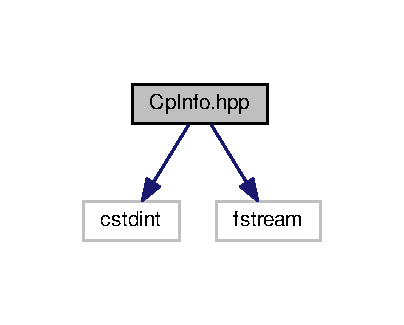
\includegraphics[width=194pt]{_cp_info_8hpp__incl}
\end{center}
\end{figure}
Este grafo mostra quais são os ficheiros que incluem directamente ou indirectamente este ficheiro\+:
\nopagebreak
\begin{figure}[H]
\begin{center}
\leavevmode
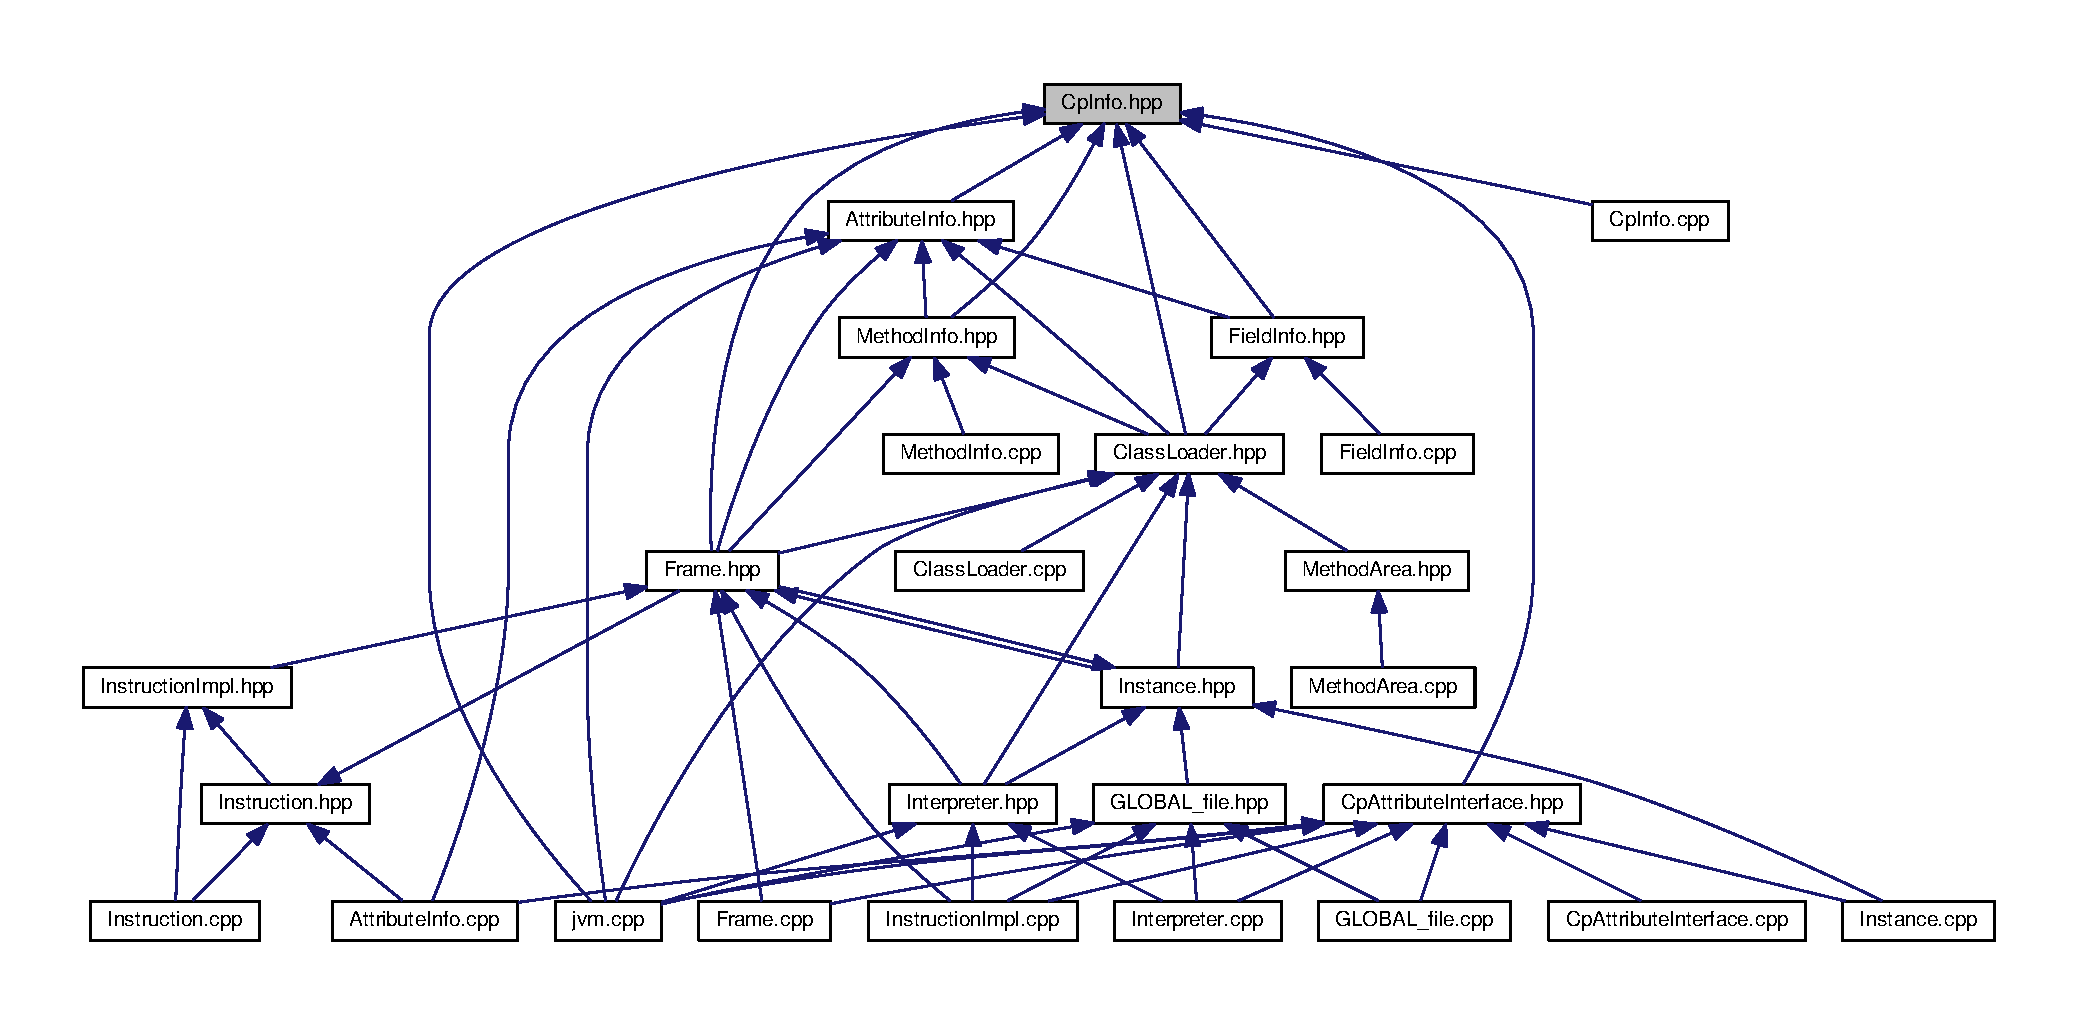
\includegraphics[width=350pt]{_cp_info_8hpp__dep__incl}
\end{center}
\end{figure}
\subsection*{Componentes}
\begin{DoxyCompactItemize}
\item 
class \hyperlink{class_cp_info}{Cp\+Info}
\begin{DoxyCompactList}\small\item\em Classe contém tag(uint8) e union que será um tipo diferente dependendo de qual tag que será passada;. \end{DoxyCompactList}\end{DoxyCompactItemize}


\subsection{Descrição detalhada}
Declarações das funções e dos atributos do Pool de constantes. 

\begin{DoxyRefDesc}{Bug}
\item[\hyperlink{bug__bug000005}{Bug}]No known bugs. \end{DoxyRefDesc}

\hypertarget{_field_info_8cpp}{}\section{Field\+Info.\+cpp File Reference}
\label{_field_info_8cpp}\index{Field\+Info.\+cpp@{Field\+Info.\+cpp}}


Funções que mexerão com as informações das fields, armazendo os mesmos a partir da leitura dos bytecodes;.  


{\ttfamily \#include \char`\"{}Field\+Info.\+hpp\char`\"{}}\\*
{\ttfamily \#include \char`\"{}Byte\+Reader.\+hpp\char`\"{}}\\*
Include dependency graph for Field\+Info.\+cpp\+:
% FIG 0


\subsection{Detailed Description}
Funções que mexerão com as informações das fields, armazendo os mesmos a partir da leitura dos bytecodes;. 


\hypertarget{_field_info_8hpp}{}\section{Referência ao ficheiro Field\+Info.\+hpp}
\label{_field_info_8hpp}\index{Field\+Info.\+hpp@{Field\+Info.\+hpp}}


Declarações das funções do \hyperlink{class_field_info}{Field\+Info} para tratamento dos fields do arquivo .class.  


{\ttfamily \#include \char`\"{}Cp\+Info.\+hpp\char`\"{}}\\*
{\ttfamily \#include \char`\"{}Attribute\+Info.\+hpp\char`\"{}}\\*
{\ttfamily \#include $<$cstdint$>$}\\*
Diagrama de dependências de inclusão para Field\+Info.\+hpp\+:
\nopagebreak
\begin{figure}[H]
\begin{center}
\leavevmode
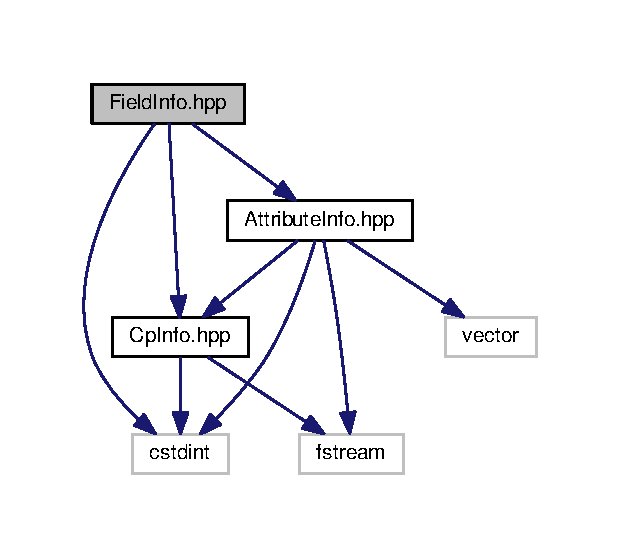
\includegraphics[width=298pt]{_field_info_8hpp__incl}
\end{center}
\end{figure}
Este grafo mostra quais são os ficheiros que incluem directamente ou indirectamente este ficheiro\+:
\nopagebreak
\begin{figure}[H]
\begin{center}
\leavevmode
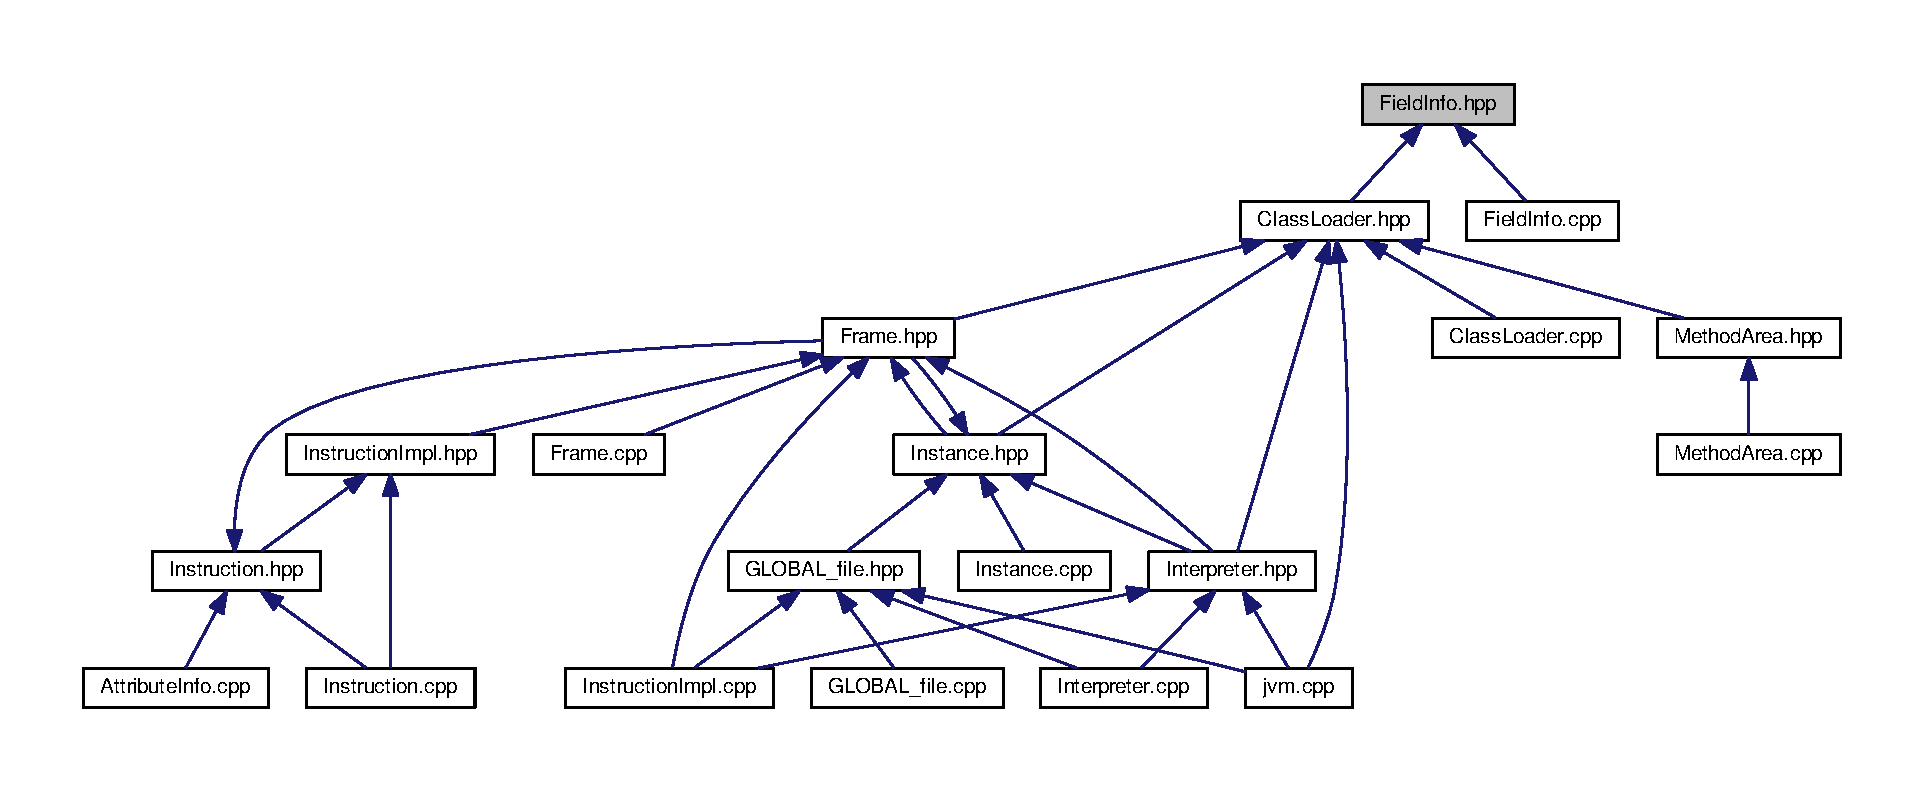
\includegraphics[width=350pt]{_field_info_8hpp__dep__incl}
\end{center}
\end{figure}
\subsection*{Componentes}
\begin{DoxyCompactItemize}
\item 
class \hyperlink{class_field_info}{Field\+Info}
\begin{DoxyCompactList}\small\item\em classe para tratar as fields do .class contém access\+\_\+flags, name\+\_\+index, descriptor\+\_\+index, attributes\+\_\+count e uma array dos atributos a ele designados -\/ tirando a array, todos do tipo uint16 Além disso contém destructor e leitor; \end{DoxyCompactList}\end{DoxyCompactItemize}


\subsection{Descrição detalhada}
Declarações das funções do \hyperlink{class_field_info}{Field\+Info} para tratamento dos fields do arquivo .class. 

\begin{DoxyRefDesc}{Bug}
\item[\hyperlink{bug__bug000006}{Bug}]No known bugs. \end{DoxyRefDesc}

\hypertarget{_frame_8cpp}{}\section{Referência ao ficheiro Frame.\+cpp}
\label{_frame_8cpp}\index{Frame.\+cpp@{Frame.\+cpp}}


Contrutor, destrutor e metodos para o funcionamento da lógica do frame;.  


{\ttfamily \#include \char`\"{}Frame.\+hpp\char`\"{}}\\*
{\ttfamily \#include \char`\"{}Cp\+Attribute\+Interface.\+hpp\char`\"{}}\\*
{\ttfamily \#include $<$iostream$>$}\\*
Diagrama de dependências de inclusão para Frame.\+cpp\+:
\nopagebreak
\begin{figure}[H]
\begin{center}
\leavevmode
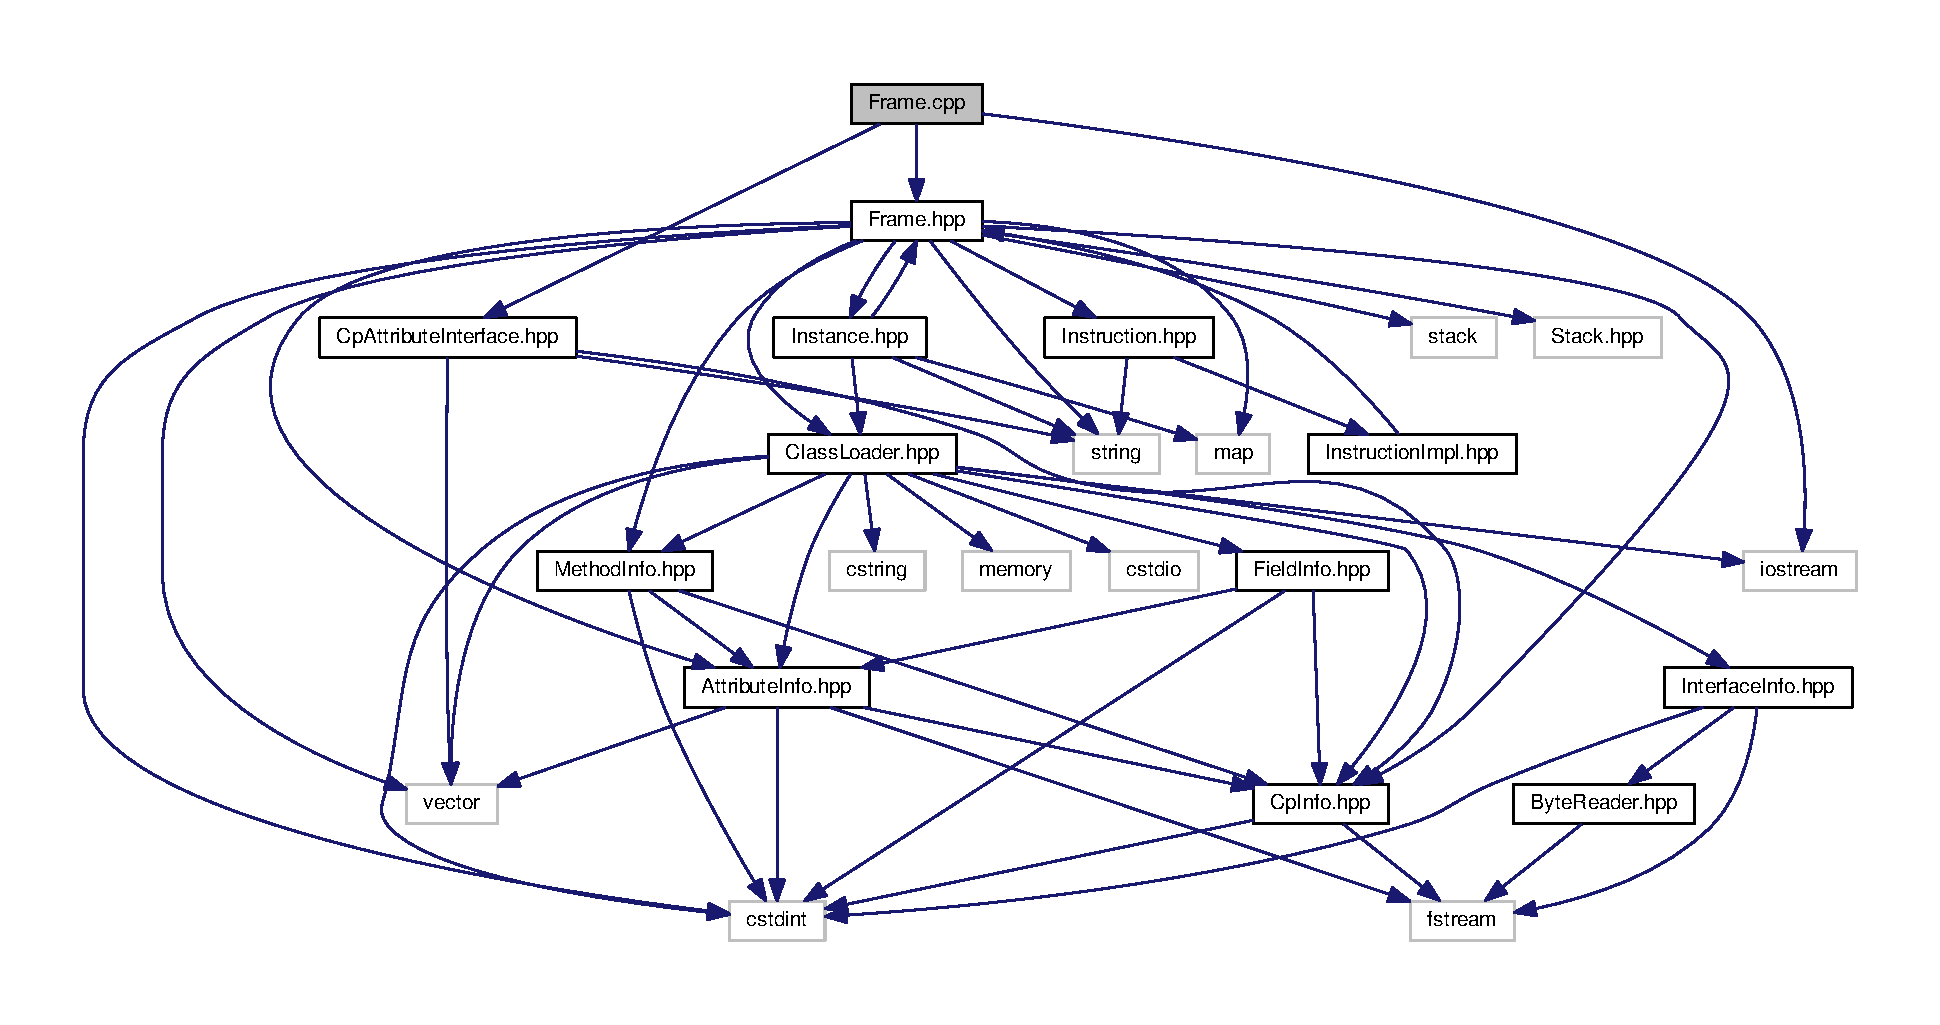
\includegraphics[width=350pt]{_frame_8cpp__incl}
\end{center}
\end{figure}


\subsection{Descrição detalhada}
Contrutor, destrutor e metodos para o funcionamento da lógica do frame;. 


\hypertarget{_frame_8hpp}{}\section{Frame.\+hpp File Reference}
\label{_frame_8hpp}\index{Frame.\+hpp@{Frame.\+hpp}}


Declarações das funções e da estrutura do \hyperlink{struct_frame}{Frame}, utilizado para salvar resultados parciais.  


{\ttfamily \#include $<$cstdint$>$}\\*
{\ttfamily \#include $<$string$>$}\\*
{\ttfamily \#include $<$vector$>$}\\*
{\ttfamily \#include $<$stack$>$}\\*
{\ttfamily \#include $<$map$>$}\\*
{\ttfamily \#include \char`\"{}Stack.\+hpp\char`\"{}}\\*
{\ttfamily \#include \char`\"{}Cp\+Info.\+hpp\char`\"{}}\\*
{\ttfamily \#include \char`\"{}Method\+Info.\+hpp\char`\"{}}\\*
{\ttfamily \#include \char`\"{}Attribute\+Info.\+hpp\char`\"{}}\\*
{\ttfamily \#include \char`\"{}Class\+Loader.\+hpp\char`\"{}}\\*
{\ttfamily \#include \char`\"{}Instruction.\+hpp\char`\"{}}\\*
{\ttfamily \#include \char`\"{}Instance.\+hpp\char`\"{}}\\*
Include dependency graph for Frame.\+hpp\+:
% FIG 0
This graph shows which files directly or indirectly include this file\+:
% FIG 1
\subsection*{Classes}
\begin{DoxyCompactItemize}
\item 
struct \hyperlink{struct_array_type}{Array\+Type}
\begin{DoxyCompactList}\small\item\em tem como base um tipo de vetor de um tipo de struct \hyperlink{struct_operand}{Operand}; \end{DoxyCompactList}\item 
struct \hyperlink{struct_operand}{Operand}
\begin{DoxyCompactList}\small\item\em intuito de ligar aos tipos possíveis para variáveis que serão utilizadas; \end{DoxyCompactList}\item 
struct \hyperlink{struct_frame}{Frame}
\begin{DoxyCompactList}\small\item\em objetivo de estruturar o tipo \hyperlink{struct_frame}{Frame}; Além disso, contém destrutor e run(para rodar o frame); \end{DoxyCompactList}\end{DoxyCompactItemize}


\subsection{Detailed Description}
Declarações das funções e da estrutura do \hyperlink{struct_frame}{Frame}, utilizado para salvar resultados parciais. 

\begin{DoxyRefDesc}{Bug}
\item[\hyperlink{bug__bug000007}{Bug}]No known bugs. \end{DoxyRefDesc}

\hypertarget{_g_l_o_b_a_l__file_8cpp}{}\section{Referência ao ficheiro G\+L\+O\+B\+A\+L\+\_\+file.\+cpp}
\label{_g_l_o_b_a_l__file_8cpp}\index{G\+L\+O\+B\+A\+L\+\_\+file.\+cpp@{G\+L\+O\+B\+A\+L\+\_\+file.\+cpp}}


Contém métodos que serão utilizados de forma global, ao invés de termos que setar o mesmo para todos os arquivos;.  


{\ttfamily \#include \char`\"{}G\+L\+O\+B\+A\+L\+\_\+file.\+hpp\char`\"{}}\\*
{\ttfamily \#include \char`\"{}Cp\+Attribute\+Interface.\+hpp\char`\"{}}\\*
Diagrama de dependências de inclusão para G\+L\+O\+B\+A\+L\+\_\+file.\+cpp\+:
\nopagebreak
\begin{figure}[H]
\begin{center}
\leavevmode
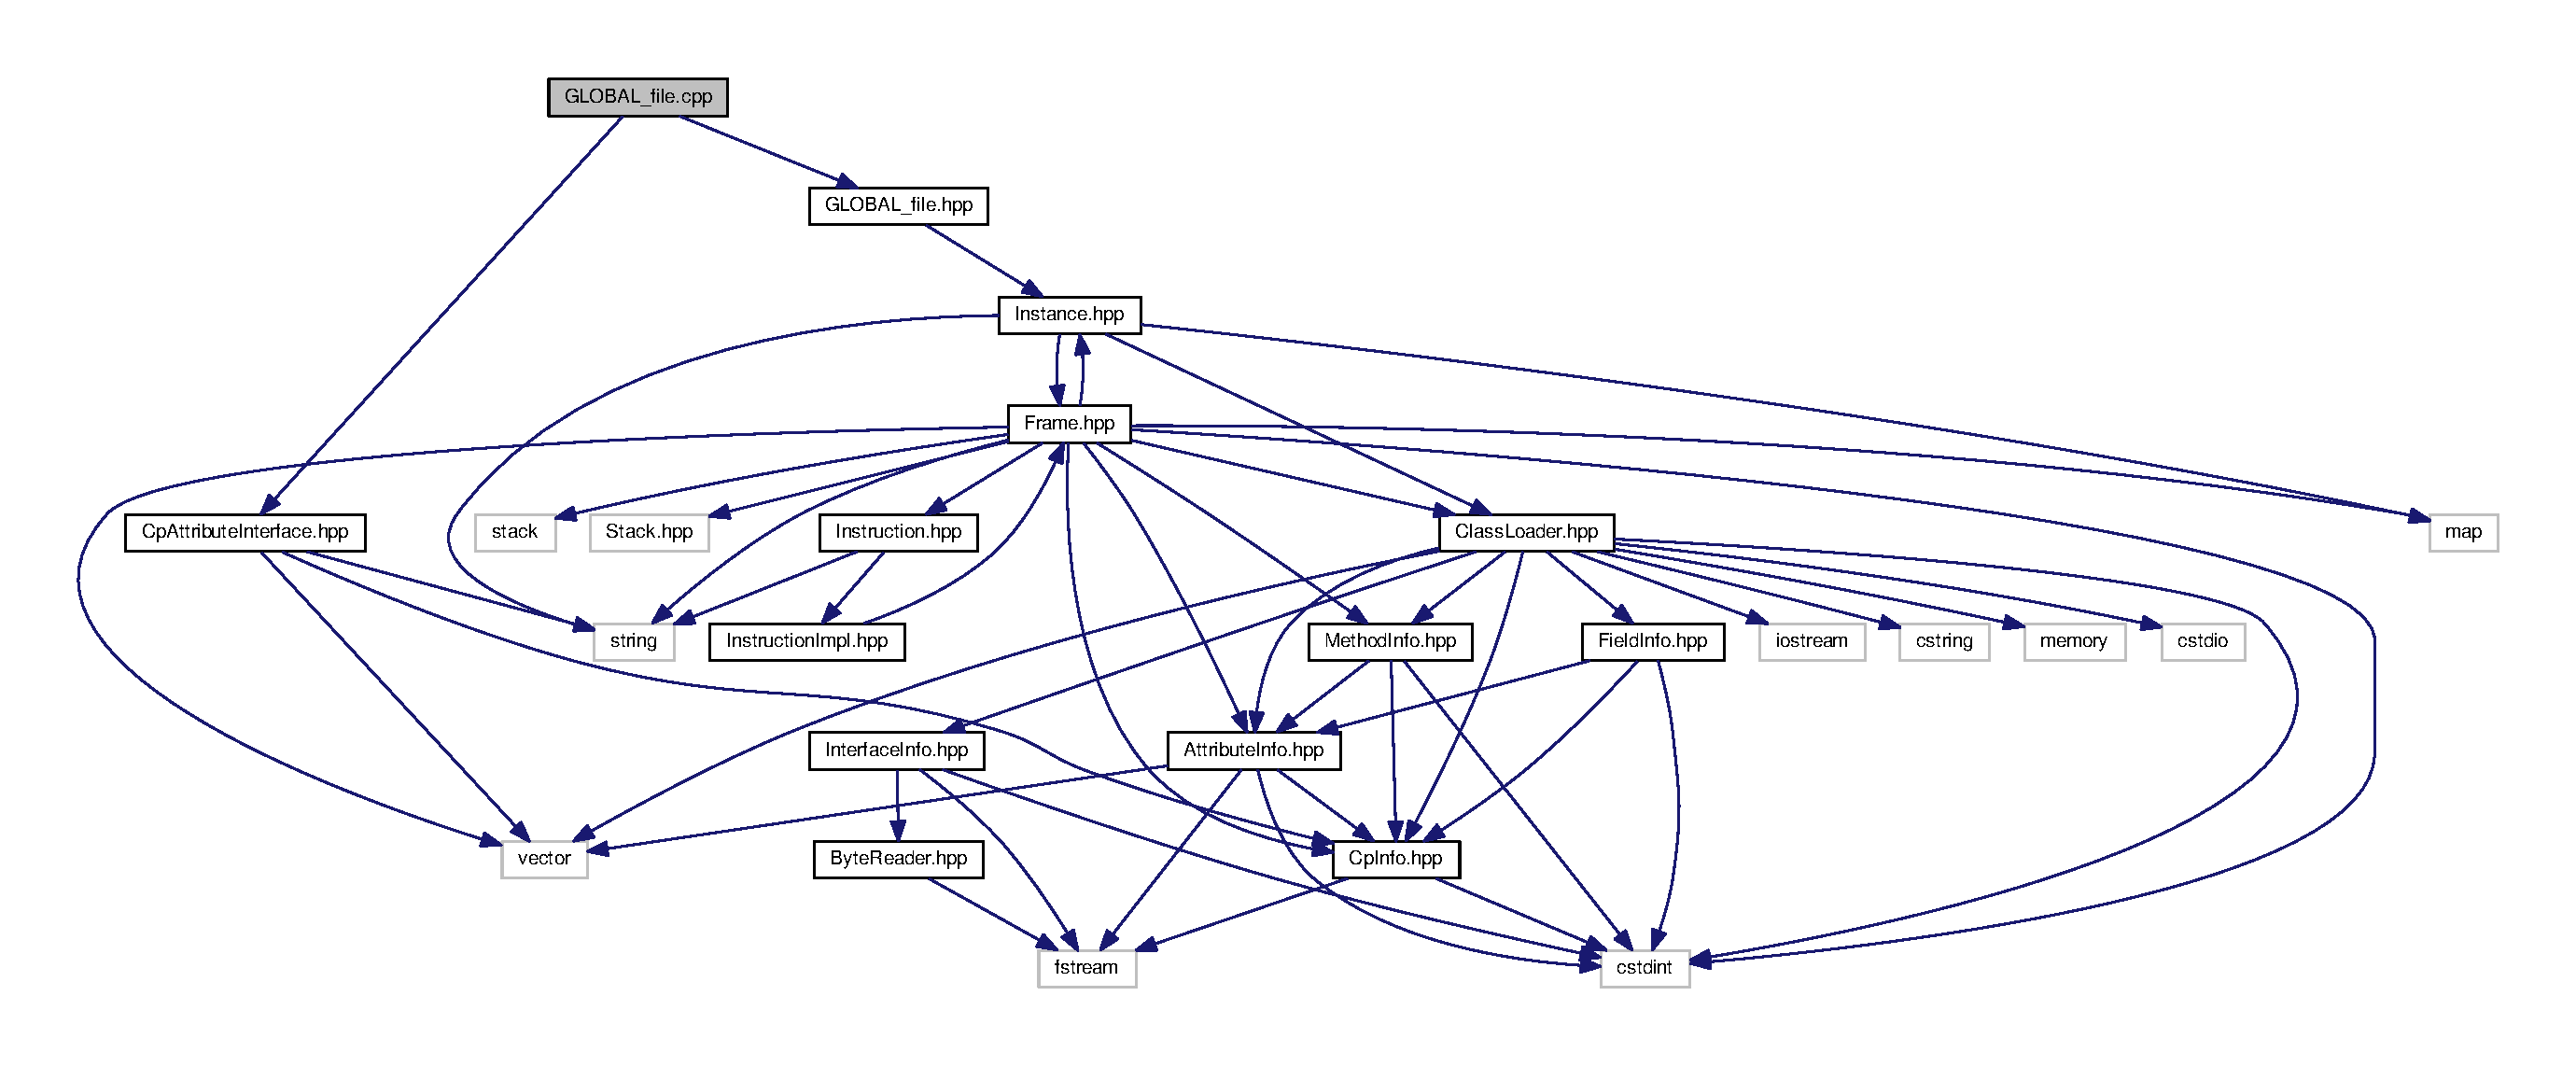
\includegraphics[width=350pt]{_g_l_o_b_a_l__file_8cpp__incl}
\end{center}
\end{figure}


\subsection{Descrição detalhada}
Contém métodos que serão utilizados de forma global, ao invés de termos que setar o mesmo para todos os arquivos;. 


\hypertarget{_g_l_o_b_a_l__file_8hpp}{}\section{Referência ao ficheiro G\+L\+O\+B\+A\+L\+\_\+file.\+hpp}
\label{_g_l_o_b_a_l__file_8hpp}\index{G\+L\+O\+B\+A\+L\+\_\+file.\+hpp@{G\+L\+O\+B\+A\+L\+\_\+file.\+hpp}}


Armazenas classes estáticas para serem usadas por todo o código.  


{\ttfamily \#include \char`\"{}Instance.\+hpp\char`\"{}}\\*
Diagrama de dependências de inclusão para G\+L\+O\+B\+A\+L\+\_\+file.\+hpp\+:
\nopagebreak
\begin{figure}[H]
\begin{center}
\leavevmode
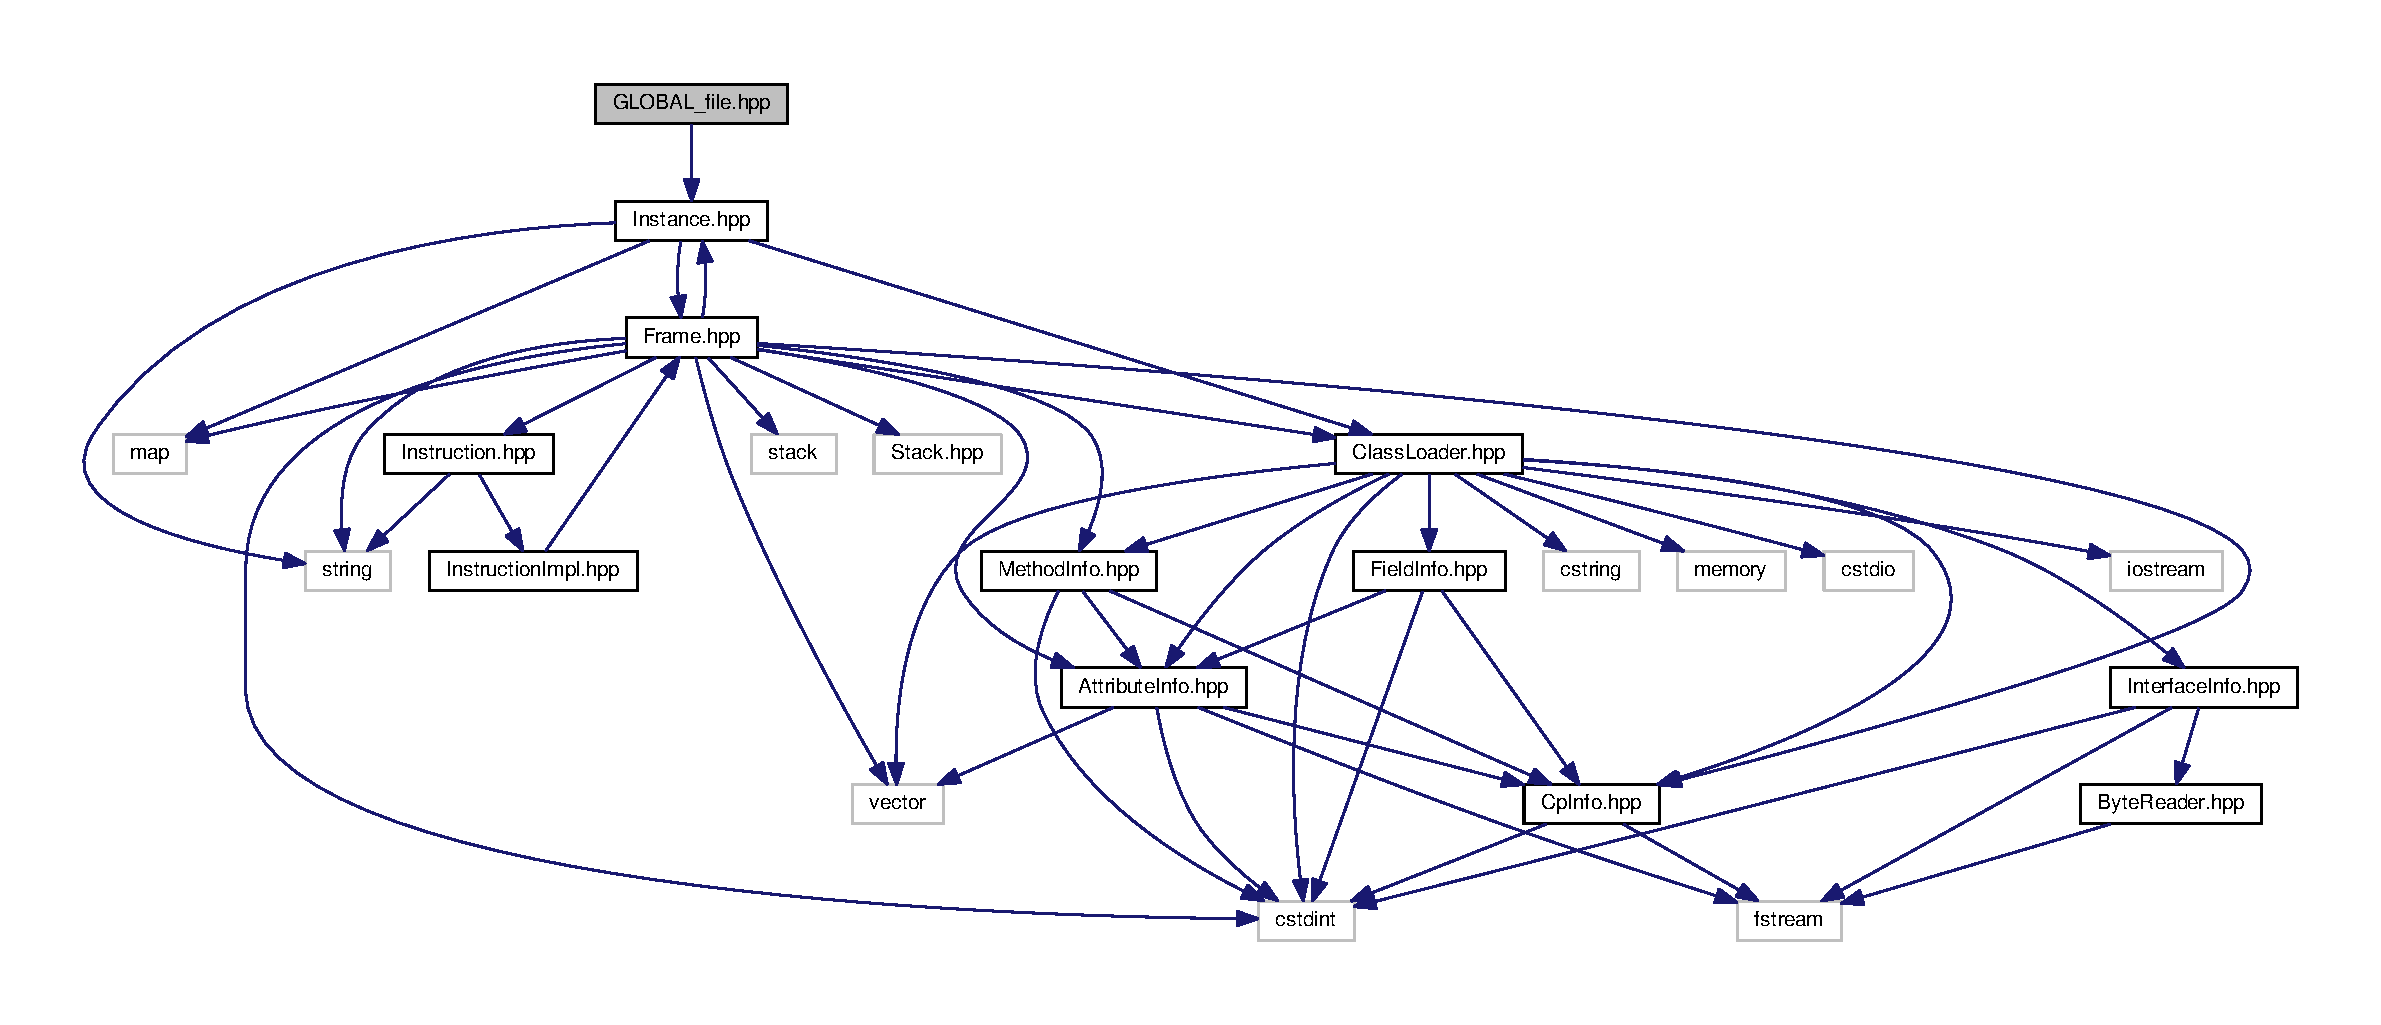
\includegraphics[width=350pt]{_g_l_o_b_a_l__file_8hpp__incl}
\end{center}
\end{figure}
Este grafo mostra quais são os ficheiros que incluem directamente ou indirectamente este ficheiro\+:
\nopagebreak
\begin{figure}[H]
\begin{center}
\leavevmode
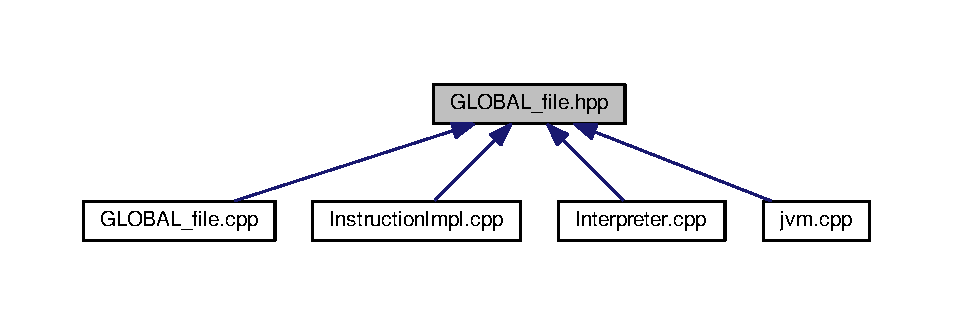
\includegraphics[width=350pt]{_g_l_o_b_a_l__file_8hpp__dep__incl}
\end{center}
\end{figure}
\subsection*{Componentes}
\begin{DoxyCompactItemize}
\item 
class \hyperlink{class_methods_area}{Methods\+Area}
\begin{DoxyCompactList}\small\item\em Armazenas classes estáticas para serem usadas por todo o código ;. \end{DoxyCompactList}\end{DoxyCompactItemize}


\subsection{Descrição detalhada}
Armazenas classes estáticas para serem usadas por todo o código. 

\begin{DoxyRefDesc}{Bug}
\item[\hyperlink{bug__bug000008}{Bug}]No known bugs. \end{DoxyRefDesc}

\hypertarget{_instance_8cpp}{}\section{Instance.\+cpp File Reference}
\label{_instance_8cpp}\index{Instance.\+cpp@{Instance.\+cpp}}


Contém métodos para carregar as informações do Classloader na Instância;.  


{\ttfamily \#include \char`\"{}Instance.\+hpp\char`\"{}}\\*
{\ttfamily \#include \char`\"{}Cp\+Attribute\+Interface.\+hpp\char`\"{}}\\*
Include dependency graph for Instance.\+cpp\+:
% FIG 0


\subsection{Detailed Description}
Contém métodos para carregar as informações do Classloader na Instância;. 


\hypertarget{_instance_8hpp}{}\section{Instance.\+hpp File Reference}
\label{_instance_8hpp}\index{Instance.\+hpp@{Instance.\+hpp}}


Declaração da struct \hyperlink{struct_instance}{Instance}.  


{\ttfamily \#include $<$map$>$}\\*
{\ttfamily \#include $<$string$>$}\\*
{\ttfamily \#include \char`\"{}Class\+Loader.\+hpp\char`\"{}}\\*
{\ttfamily \#include \char`\"{}Frame.\+hpp\char`\"{}}\\*
Include dependency graph for Instance.\+hpp\+:
% FIG 0
This graph shows which files directly or indirectly include this file\+:
% FIG 1
\subsection*{Classes}
\begin{DoxyCompactItemize}
\item 
struct \hyperlink{struct_instance}{Instance}
\begin{DoxyCompactList}\small\item\em tipo que determinará o nome e o tipo de operando através do \hyperlink{struct_operand}{Operand} class; Álém contém o método \hyperlink{class_instance_1_1_instance}{Instance\+::\+Instance} \end{DoxyCompactList}\end{DoxyCompactItemize}


\subsection{Detailed Description}
Declaração da struct \hyperlink{struct_instance}{Instance}. 

\begin{DoxyRefDesc}{Bug}
\item[\hyperlink{bug__bug000009}{Bug}]No known bugs. \end{DoxyRefDesc}

\hypertarget{_instruction_8cpp}{}\section{Instruction.\+cpp File Reference}
\label{_instruction_8cpp}\index{Instruction.\+cpp@{Instruction.\+cpp}}


Métodos que servem para inicializar todas as intruções contidas na documentação;.  


{\ttfamily \#include \char`\"{}Instruction.\+hpp\char`\"{}}\\*
{\ttfamily \#include \char`\"{}Instruction\+Impl.\+hpp\char`\"{}}\\*
{\ttfamily \#include $<$iostream$>$}\\*
Include dependency graph for Instruction.\+cpp\+:
% FIG 0


\subsection{Detailed Description}
Métodos que servem para inicializar todas as intruções contidas na documentação;. 


\hypertarget{_instruction_8hpp}{}\section{Referência ao ficheiro Instruction.\+hpp}
\label{_instruction_8hpp}\index{Instruction.\+hpp@{Instruction.\+hpp}}


Declarações das instruçoes referentes ao interpretador da J\+VM.  


{\ttfamily \#include $<$string$>$}\\*
{\ttfamily \#include \char`\"{}Instruction\+Impl.\+hpp\char`\"{}}\\*
Diagrama de dependências de inclusão para Instruction.\+hpp\+:
\nopagebreak
\begin{figure}[H]
\begin{center}
\leavevmode
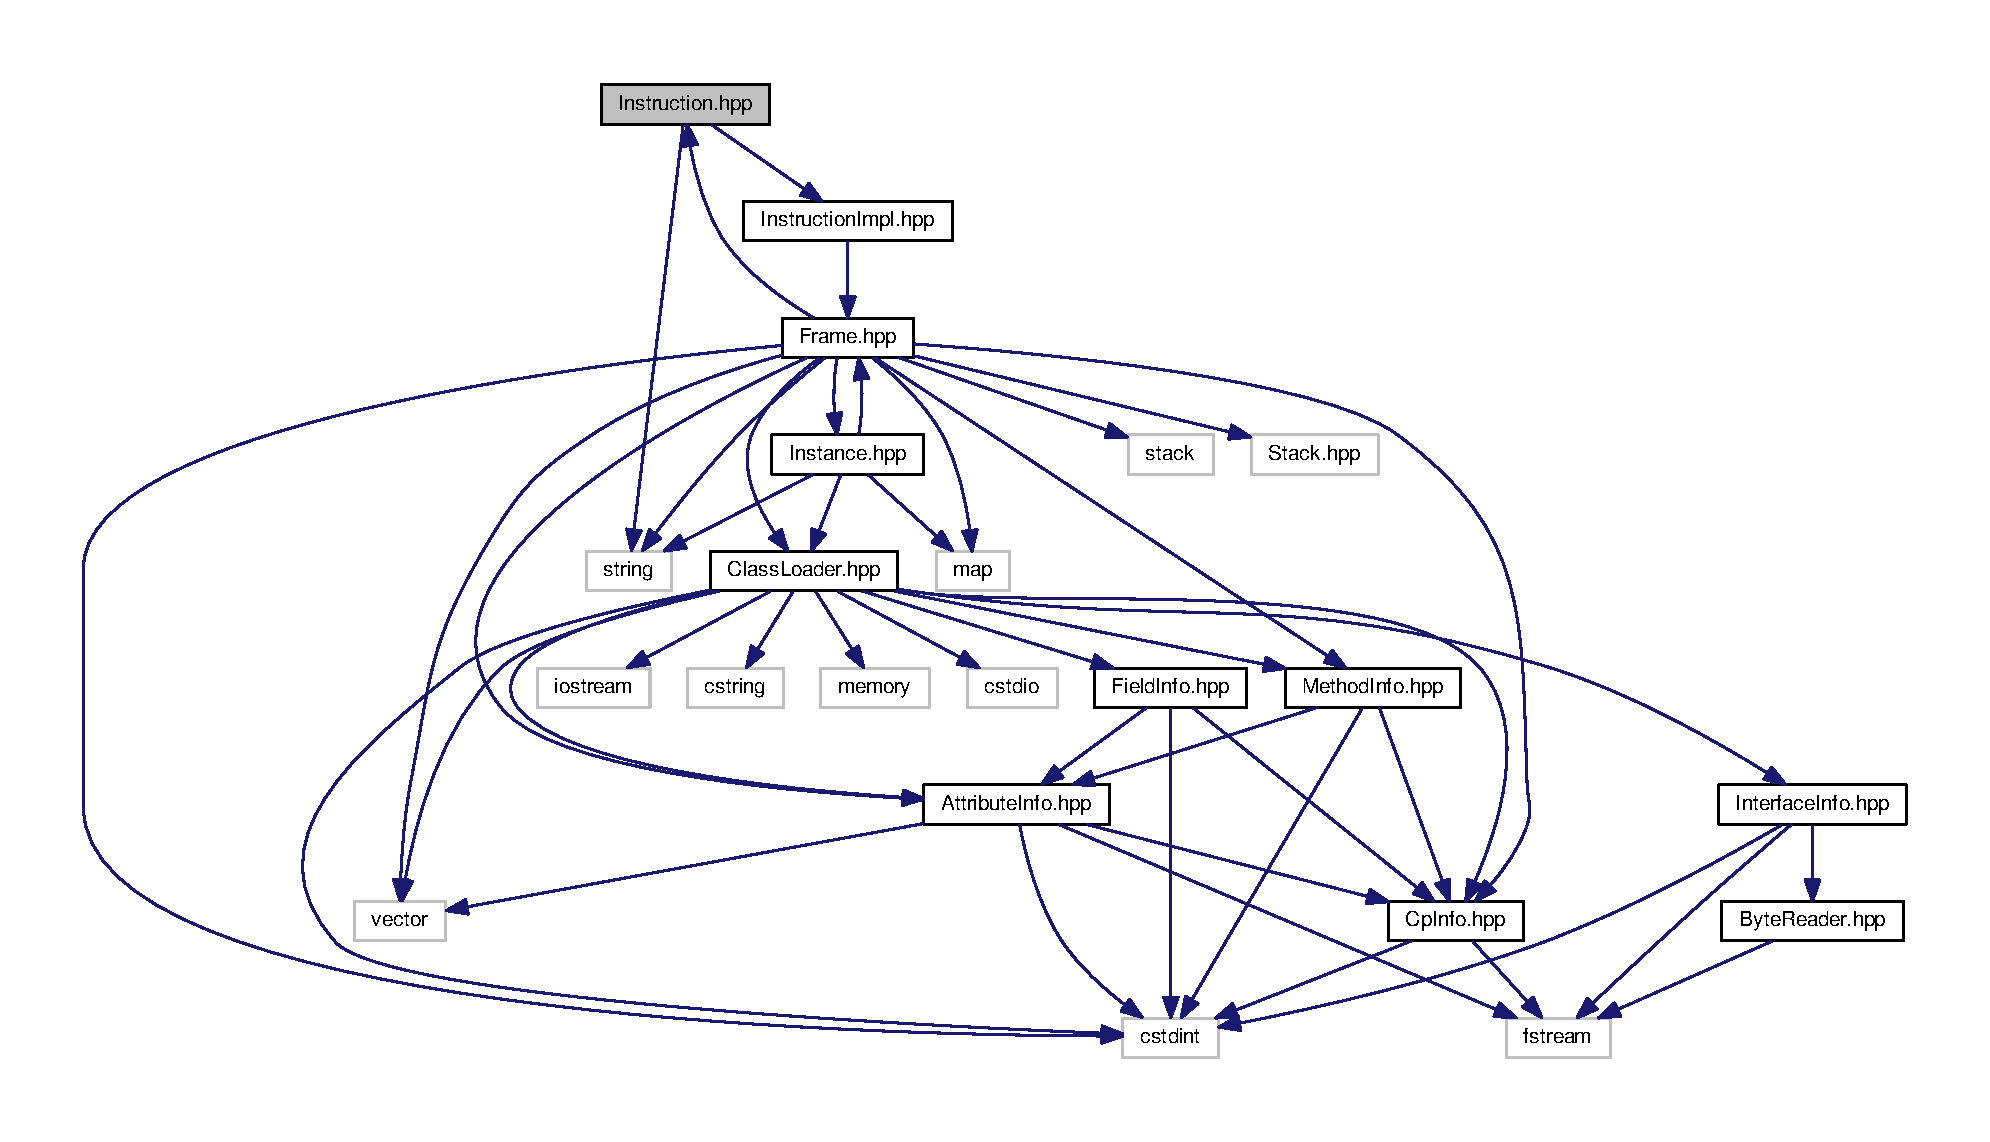
\includegraphics[width=350pt]{_instruction_8hpp__incl}
\end{center}
\end{figure}
Este grafo mostra quais são os ficheiros que incluem directamente ou indirectamente este ficheiro\+:
\nopagebreak
\begin{figure}[H]
\begin{center}
\leavevmode
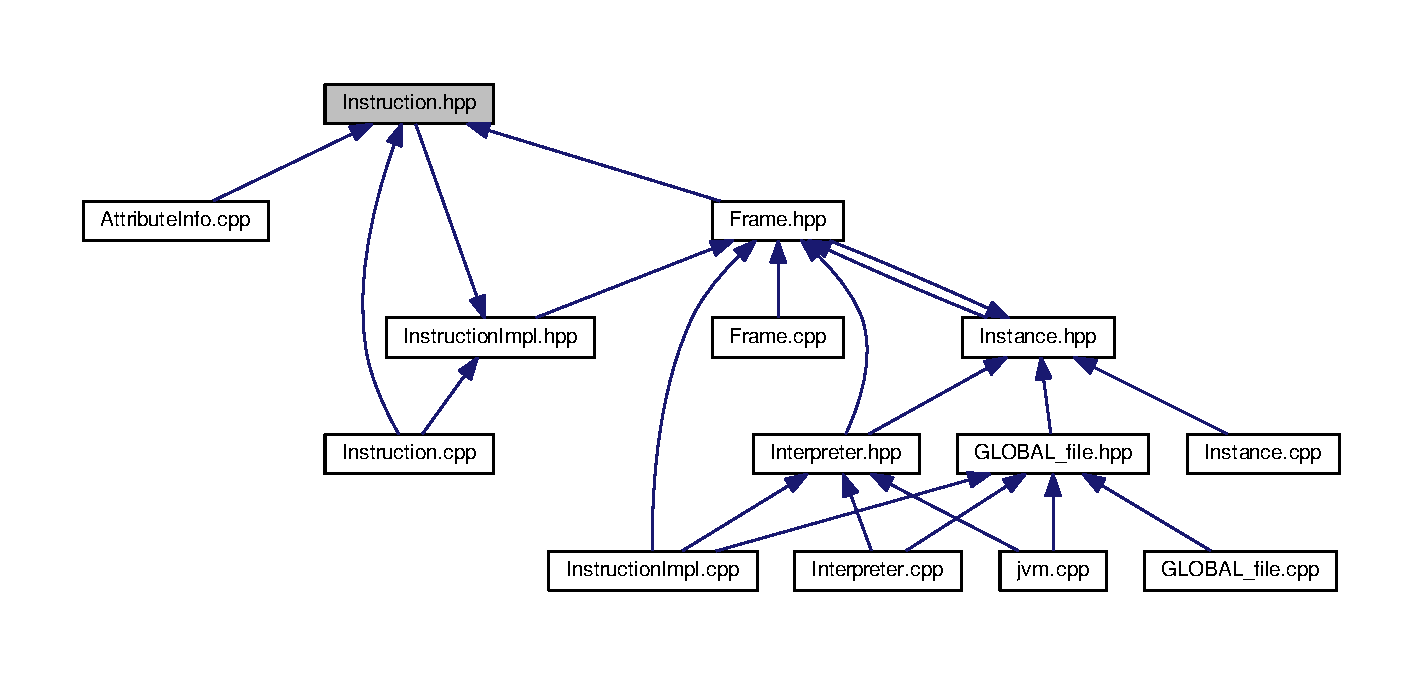
\includegraphics[width=350pt]{_instruction_8hpp__dep__incl}
\end{center}
\end{figure}
\subsection*{Componentes}
\begin{DoxyCompactItemize}
\item 
class \hyperlink{class_instruction}{Instruction}
\begin{DoxyCompactList}\small\item\em Determina a instrução de acordo com o interpretador;. \end{DoxyCompactList}\end{DoxyCompactItemize}
\subsection*{Macros}
\begin{DoxyCompactItemize}
\item 
\#define \hyperlink{_instruction_8hpp_af024387d0f45d9734e7556f54a2384a5}{c\+\_\+newarray}~188
\item 
\#define \hyperlink{_instruction_8hpp_a3b7425744f6fd415140ce716d838a4fd}{c\+\_\+anewarray}~189
\item 
\#define \hyperlink{_instruction_8hpp_a09979a42bf87fbc3177e382cebbaee19}{c\+\_\+multianewarray}~197
\item 
\#define \hyperlink{_instruction_8hpp_a90a73b8de141cd93e0c259c503fee010}{c\+\_\+checkcast}~192
\item 
\#define \hyperlink{_instruction_8hpp_a3cfa7ec97de2d289052ddd0680abdfb4}{c\+\_\+getfield}~180
\item 
\#define \hyperlink{_instruction_8hpp_ae8a6149f585c51e4b444217e87b693bb}{c\+\_\+getstatic}~178
\item 
\#define \hyperlink{_instruction_8hpp_a702714f5ee59249adb4ab9bf75861208}{c\+\_\+instanceof}~193
\item 
\#define \hyperlink{_instruction_8hpp_a347479ae665fc03bb9164ba69e24ea4f}{c\+\_\+invokedynamic}~186
\item 
\#define \hyperlink{_instruction_8hpp_a246619600268eb4350974cfcd418f489}{c\+\_\+invokeinterface}~185
\item 
\#define \hyperlink{_instruction_8hpp_a51ed58121489d1657589a6fbe6bfc3ee}{c\+\_\+invokespecial}~183
\item 
\#define \hyperlink{_instruction_8hpp_a85ea809f4c00c5c86e41658983f1f2c0}{c\+\_\+invokestatic}~184
\item 
\#define \hyperlink{_instruction_8hpp_af55698fdc4f0dc27a68374ef0fbee5b7}{c\+\_\+invokevirtual}~182
\item 
\#define \hyperlink{_instruction_8hpp_af6007cb94388a9e17608316d6f680c0e}{c\+\_\+ldc}~18
\item 
\#define \hyperlink{_instruction_8hpp_ae5cd40314d84ebeee2f9dc219c6a4188}{c\+\_\+ldc\+\_\+w}~19
\item 
\#define \hyperlink{_instruction_8hpp_add4ed29add2ba9318a75c81ee75b5952}{c\+\_\+ldc2\+\_\+w}~20
\item 
\#define \hyperlink{_instruction_8hpp_a1031ff1614a44c06c2c2207c6622c2ce}{c\+\_\+\+N\+EW}~187
\item 
\#define \hyperlink{_instruction_8hpp_ad60c7634d75a3b2bfbd21cc9956242fd}{c\+\_\+putfield}~181
\item 
\#define \hyperlink{_instruction_8hpp_a6f69546da54368a6ea41d5b640979157}{c\+\_\+putstatic}~179
\item 
\#define \hyperlink{_instruction_8hpp_aa05f11a780cb9e97da01c7f76b052def}{c\+\_\+\+G\+O\+TO}~167
\item 
\#define \hyperlink{_instruction_8hpp_a6dea4dcd35e14bbcd7092e259a371fc3}{c\+\_\+if\+\_\+acmpeq}~165
\item 
\#define \hyperlink{_instruction_8hpp_a4900bb229a44b6aba9e80b34089f98fe}{c\+\_\+if\+\_\+acmpne}~166
\item 
\#define \hyperlink{_instruction_8hpp_ab3cbd9f13a3dfffbfca77df161b91afc}{c\+\_\+if\+\_\+icmpeq}~159
\item 
\#define \hyperlink{_instruction_8hpp_a9d23d6274551d4d6412ffb73cb1414a0}{c\+\_\+if\+\_\+icmpne}~160
\item 
\#define \hyperlink{_instruction_8hpp_a9216eea0da2497c8eb898d813b6659f7}{c\+\_\+if\+\_\+icmplt}~161
\item 
\#define \hyperlink{_instruction_8hpp_a7ffce2f98e9cc726e565aed0fd8145f1}{c\+\_\+if\+\_\+icmpge}~162
\item 
\#define \hyperlink{_instruction_8hpp_ac4686ce482d6bdb7841705f21c180fad}{c\+\_\+if\+\_\+icmpgt}~163
\item 
\#define \hyperlink{_instruction_8hpp_ae5659c7561f340394f1abaa947cf3572}{c\+\_\+if\+\_\+icmple}~164
\item 
\#define \hyperlink{_instruction_8hpp_a82fbda9e87966b4381af74fc3f456836}{c\+\_\+iifeq}~153
\item 
\#define \hyperlink{_instruction_8hpp_a7d225b039764c13b0ce5d5a28c195f39}{c\+\_\+ifne}~154
\item 
\#define \hyperlink{_instruction_8hpp_a1090209aa6bce5f0d37c5f23a9249ccf}{c\+\_\+iflt}~155
\item 
\#define \hyperlink{_instruction_8hpp_aa70bd676cddda2e21b84dac68de86920}{c\+\_\+ifge}~156
\item 
\#define \hyperlink{_instruction_8hpp_af67ebddc8c9dce24bb254e9c398a4123}{c\+\_\+ifgt}~157
\item 
\#define \hyperlink{_instruction_8hpp_a6609d5282f39b2055658a729c0df3416}{c\+\_\+ifle}~158
\item 
\#define \hyperlink{_instruction_8hpp_a84125ce1fe99f18501915a62a407495a}{c\+\_\+ifnonull}~199
\item 
\#define \hyperlink{_instruction_8hpp_abe88ae981e276a8a704638b0c8d10aba}{c\+\_\+ifnull}~198
\item 
\#define \hyperlink{_instruction_8hpp_a466b083b129d9f6e48c9d49b13bfef05}{c\+\_\+jsr}~168
\item 
\#define \hyperlink{_instruction_8hpp_a0700b0699b50c56f67dfd396d88f2c3a}{c\+\_\+aload}~25
\item 
\#define \hyperlink{_instruction_8hpp_a3c9ea503e41241986905dadde5185f0b}{c\+\_\+aload\+\_\+0}~42
\item 
\#define \hyperlink{_instruction_8hpp_a9a0733d50a7571e57306116029be020c}{c\+\_\+aload\+\_\+1}~43
\item 
\#define \hyperlink{_instruction_8hpp_af9e083e956d77cf9156022f36f64c9e0}{c\+\_\+aload\+\_\+2}~44
\item 
\#define \hyperlink{_instruction_8hpp_aa1a345c2213daf53b2dea916bd0b5380}{c\+\_\+aload\+\_\+3}~45
\item 
\#define \hyperlink{_instruction_8hpp_aca9fac7340c1cfa658f7a6e0fe7d67fe}{c\+\_\+areturn}~176
\item 
\#define \hyperlink{_instruction_8hpp_afc06f3626ec61b868b7f04b2fc7d58a6}{c\+\_\+return\+\_\+original}~177
\end{DoxyCompactItemize}


\subsection{Descrição detalhada}
Declarações das instruçoes referentes ao interpretador da J\+VM. 

\begin{DoxyRefDesc}{Bug}
\item[\hyperlink{bug__bug000010}{Bug}]No known bugs. \end{DoxyRefDesc}


\subsection{Documentação das macros}
\index{Instruction.\+hpp@{Instruction.\+hpp}!c\+\_\+aload@{c\+\_\+aload}}
\index{c\+\_\+aload@{c\+\_\+aload}!Instruction.\+hpp@{Instruction.\+hpp}}
\subsubsection[{\texorpdfstring{c\+\_\+aload}{c_aload}}]{\setlength{\rightskip}{0pt plus 5cm}\#define c\+\_\+aload~25}\hypertarget{_instruction_8hpp_a0700b0699b50c56f67dfd396d88f2c3a}{}\label{_instruction_8hpp_a0700b0699b50c56f67dfd396d88f2c3a}
\index{Instruction.\+hpp@{Instruction.\+hpp}!c\+\_\+aload\+\_\+0@{c\+\_\+aload\+\_\+0}}
\index{c\+\_\+aload\+\_\+0@{c\+\_\+aload\+\_\+0}!Instruction.\+hpp@{Instruction.\+hpp}}
\subsubsection[{\texorpdfstring{c\+\_\+aload\+\_\+0}{c_aload_0}}]{\setlength{\rightskip}{0pt plus 5cm}\#define c\+\_\+aload\+\_\+0~42}\hypertarget{_instruction_8hpp_a3c9ea503e41241986905dadde5185f0b}{}\label{_instruction_8hpp_a3c9ea503e41241986905dadde5185f0b}
\index{Instruction.\+hpp@{Instruction.\+hpp}!c\+\_\+aload\+\_\+1@{c\+\_\+aload\+\_\+1}}
\index{c\+\_\+aload\+\_\+1@{c\+\_\+aload\+\_\+1}!Instruction.\+hpp@{Instruction.\+hpp}}
\subsubsection[{\texorpdfstring{c\+\_\+aload\+\_\+1}{c_aload_1}}]{\setlength{\rightskip}{0pt plus 5cm}\#define c\+\_\+aload\+\_\+1~43}\hypertarget{_instruction_8hpp_a9a0733d50a7571e57306116029be020c}{}\label{_instruction_8hpp_a9a0733d50a7571e57306116029be020c}
\index{Instruction.\+hpp@{Instruction.\+hpp}!c\+\_\+aload\+\_\+2@{c\+\_\+aload\+\_\+2}}
\index{c\+\_\+aload\+\_\+2@{c\+\_\+aload\+\_\+2}!Instruction.\+hpp@{Instruction.\+hpp}}
\subsubsection[{\texorpdfstring{c\+\_\+aload\+\_\+2}{c_aload_2}}]{\setlength{\rightskip}{0pt plus 5cm}\#define c\+\_\+aload\+\_\+2~44}\hypertarget{_instruction_8hpp_af9e083e956d77cf9156022f36f64c9e0}{}\label{_instruction_8hpp_af9e083e956d77cf9156022f36f64c9e0}
\index{Instruction.\+hpp@{Instruction.\+hpp}!c\+\_\+aload\+\_\+3@{c\+\_\+aload\+\_\+3}}
\index{c\+\_\+aload\+\_\+3@{c\+\_\+aload\+\_\+3}!Instruction.\+hpp@{Instruction.\+hpp}}
\subsubsection[{\texorpdfstring{c\+\_\+aload\+\_\+3}{c_aload_3}}]{\setlength{\rightskip}{0pt plus 5cm}\#define c\+\_\+aload\+\_\+3~45}\hypertarget{_instruction_8hpp_aa1a345c2213daf53b2dea916bd0b5380}{}\label{_instruction_8hpp_aa1a345c2213daf53b2dea916bd0b5380}
\index{Instruction.\+hpp@{Instruction.\+hpp}!c\+\_\+anewarray@{c\+\_\+anewarray}}
\index{c\+\_\+anewarray@{c\+\_\+anewarray}!Instruction.\+hpp@{Instruction.\+hpp}}
\subsubsection[{\texorpdfstring{c\+\_\+anewarray}{c_anewarray}}]{\setlength{\rightskip}{0pt plus 5cm}\#define c\+\_\+anewarray~189}\hypertarget{_instruction_8hpp_a3b7425744f6fd415140ce716d838a4fd}{}\label{_instruction_8hpp_a3b7425744f6fd415140ce716d838a4fd}
\index{Instruction.\+hpp@{Instruction.\+hpp}!c\+\_\+areturn@{c\+\_\+areturn}}
\index{c\+\_\+areturn@{c\+\_\+areturn}!Instruction.\+hpp@{Instruction.\+hpp}}
\subsubsection[{\texorpdfstring{c\+\_\+areturn}{c_areturn}}]{\setlength{\rightskip}{0pt plus 5cm}\#define c\+\_\+areturn~176}\hypertarget{_instruction_8hpp_aca9fac7340c1cfa658f7a6e0fe7d67fe}{}\label{_instruction_8hpp_aca9fac7340c1cfa658f7a6e0fe7d67fe}
\index{Instruction.\+hpp@{Instruction.\+hpp}!c\+\_\+checkcast@{c\+\_\+checkcast}}
\index{c\+\_\+checkcast@{c\+\_\+checkcast}!Instruction.\+hpp@{Instruction.\+hpp}}
\subsubsection[{\texorpdfstring{c\+\_\+checkcast}{c_checkcast}}]{\setlength{\rightskip}{0pt plus 5cm}\#define c\+\_\+checkcast~192}\hypertarget{_instruction_8hpp_a90a73b8de141cd93e0c259c503fee010}{}\label{_instruction_8hpp_a90a73b8de141cd93e0c259c503fee010}
\index{Instruction.\+hpp@{Instruction.\+hpp}!c\+\_\+getfield@{c\+\_\+getfield}}
\index{c\+\_\+getfield@{c\+\_\+getfield}!Instruction.\+hpp@{Instruction.\+hpp}}
\subsubsection[{\texorpdfstring{c\+\_\+getfield}{c_getfield}}]{\setlength{\rightskip}{0pt plus 5cm}\#define c\+\_\+getfield~180}\hypertarget{_instruction_8hpp_a3cfa7ec97de2d289052ddd0680abdfb4}{}\label{_instruction_8hpp_a3cfa7ec97de2d289052ddd0680abdfb4}
\index{Instruction.\+hpp@{Instruction.\+hpp}!c\+\_\+getstatic@{c\+\_\+getstatic}}
\index{c\+\_\+getstatic@{c\+\_\+getstatic}!Instruction.\+hpp@{Instruction.\+hpp}}
\subsubsection[{\texorpdfstring{c\+\_\+getstatic}{c_getstatic}}]{\setlength{\rightskip}{0pt plus 5cm}\#define c\+\_\+getstatic~178}\hypertarget{_instruction_8hpp_ae8a6149f585c51e4b444217e87b693bb}{}\label{_instruction_8hpp_ae8a6149f585c51e4b444217e87b693bb}
\index{Instruction.\+hpp@{Instruction.\+hpp}!c\+\_\+\+G\+O\+TO@{c\+\_\+\+G\+O\+TO}}
\index{c\+\_\+\+G\+O\+TO@{c\+\_\+\+G\+O\+TO}!Instruction.\+hpp@{Instruction.\+hpp}}
\subsubsection[{\texorpdfstring{c\+\_\+\+G\+O\+TO}{c_GOTO}}]{\setlength{\rightskip}{0pt plus 5cm}\#define c\+\_\+\+G\+O\+TO~167}\hypertarget{_instruction_8hpp_aa05f11a780cb9e97da01c7f76b052def}{}\label{_instruction_8hpp_aa05f11a780cb9e97da01c7f76b052def}
\index{Instruction.\+hpp@{Instruction.\+hpp}!c\+\_\+if\+\_\+acmpeq@{c\+\_\+if\+\_\+acmpeq}}
\index{c\+\_\+if\+\_\+acmpeq@{c\+\_\+if\+\_\+acmpeq}!Instruction.\+hpp@{Instruction.\+hpp}}
\subsubsection[{\texorpdfstring{c\+\_\+if\+\_\+acmpeq}{c_if_acmpeq}}]{\setlength{\rightskip}{0pt plus 5cm}\#define c\+\_\+if\+\_\+acmpeq~165}\hypertarget{_instruction_8hpp_a6dea4dcd35e14bbcd7092e259a371fc3}{}\label{_instruction_8hpp_a6dea4dcd35e14bbcd7092e259a371fc3}
\index{Instruction.\+hpp@{Instruction.\+hpp}!c\+\_\+if\+\_\+acmpne@{c\+\_\+if\+\_\+acmpne}}
\index{c\+\_\+if\+\_\+acmpne@{c\+\_\+if\+\_\+acmpne}!Instruction.\+hpp@{Instruction.\+hpp}}
\subsubsection[{\texorpdfstring{c\+\_\+if\+\_\+acmpne}{c_if_acmpne}}]{\setlength{\rightskip}{0pt plus 5cm}\#define c\+\_\+if\+\_\+acmpne~166}\hypertarget{_instruction_8hpp_a4900bb229a44b6aba9e80b34089f98fe}{}\label{_instruction_8hpp_a4900bb229a44b6aba9e80b34089f98fe}
\index{Instruction.\+hpp@{Instruction.\+hpp}!c\+\_\+if\+\_\+icmpeq@{c\+\_\+if\+\_\+icmpeq}}
\index{c\+\_\+if\+\_\+icmpeq@{c\+\_\+if\+\_\+icmpeq}!Instruction.\+hpp@{Instruction.\+hpp}}
\subsubsection[{\texorpdfstring{c\+\_\+if\+\_\+icmpeq}{c_if_icmpeq}}]{\setlength{\rightskip}{0pt plus 5cm}\#define c\+\_\+if\+\_\+icmpeq~159}\hypertarget{_instruction_8hpp_ab3cbd9f13a3dfffbfca77df161b91afc}{}\label{_instruction_8hpp_ab3cbd9f13a3dfffbfca77df161b91afc}
\index{Instruction.\+hpp@{Instruction.\+hpp}!c\+\_\+if\+\_\+icmpge@{c\+\_\+if\+\_\+icmpge}}
\index{c\+\_\+if\+\_\+icmpge@{c\+\_\+if\+\_\+icmpge}!Instruction.\+hpp@{Instruction.\+hpp}}
\subsubsection[{\texorpdfstring{c\+\_\+if\+\_\+icmpge}{c_if_icmpge}}]{\setlength{\rightskip}{0pt plus 5cm}\#define c\+\_\+if\+\_\+icmpge~162}\hypertarget{_instruction_8hpp_a7ffce2f98e9cc726e565aed0fd8145f1}{}\label{_instruction_8hpp_a7ffce2f98e9cc726e565aed0fd8145f1}
\index{Instruction.\+hpp@{Instruction.\+hpp}!c\+\_\+if\+\_\+icmpgt@{c\+\_\+if\+\_\+icmpgt}}
\index{c\+\_\+if\+\_\+icmpgt@{c\+\_\+if\+\_\+icmpgt}!Instruction.\+hpp@{Instruction.\+hpp}}
\subsubsection[{\texorpdfstring{c\+\_\+if\+\_\+icmpgt}{c_if_icmpgt}}]{\setlength{\rightskip}{0pt plus 5cm}\#define c\+\_\+if\+\_\+icmpgt~163}\hypertarget{_instruction_8hpp_ac4686ce482d6bdb7841705f21c180fad}{}\label{_instruction_8hpp_ac4686ce482d6bdb7841705f21c180fad}
\index{Instruction.\+hpp@{Instruction.\+hpp}!c\+\_\+if\+\_\+icmple@{c\+\_\+if\+\_\+icmple}}
\index{c\+\_\+if\+\_\+icmple@{c\+\_\+if\+\_\+icmple}!Instruction.\+hpp@{Instruction.\+hpp}}
\subsubsection[{\texorpdfstring{c\+\_\+if\+\_\+icmple}{c_if_icmple}}]{\setlength{\rightskip}{0pt plus 5cm}\#define c\+\_\+if\+\_\+icmple~164}\hypertarget{_instruction_8hpp_ae5659c7561f340394f1abaa947cf3572}{}\label{_instruction_8hpp_ae5659c7561f340394f1abaa947cf3572}
\index{Instruction.\+hpp@{Instruction.\+hpp}!c\+\_\+if\+\_\+icmplt@{c\+\_\+if\+\_\+icmplt}}
\index{c\+\_\+if\+\_\+icmplt@{c\+\_\+if\+\_\+icmplt}!Instruction.\+hpp@{Instruction.\+hpp}}
\subsubsection[{\texorpdfstring{c\+\_\+if\+\_\+icmplt}{c_if_icmplt}}]{\setlength{\rightskip}{0pt plus 5cm}\#define c\+\_\+if\+\_\+icmplt~161}\hypertarget{_instruction_8hpp_a9216eea0da2497c8eb898d813b6659f7}{}\label{_instruction_8hpp_a9216eea0da2497c8eb898d813b6659f7}
\index{Instruction.\+hpp@{Instruction.\+hpp}!c\+\_\+if\+\_\+icmpne@{c\+\_\+if\+\_\+icmpne}}
\index{c\+\_\+if\+\_\+icmpne@{c\+\_\+if\+\_\+icmpne}!Instruction.\+hpp@{Instruction.\+hpp}}
\subsubsection[{\texorpdfstring{c\+\_\+if\+\_\+icmpne}{c_if_icmpne}}]{\setlength{\rightskip}{0pt plus 5cm}\#define c\+\_\+if\+\_\+icmpne~160}\hypertarget{_instruction_8hpp_a9d23d6274551d4d6412ffb73cb1414a0}{}\label{_instruction_8hpp_a9d23d6274551d4d6412ffb73cb1414a0}
\index{Instruction.\+hpp@{Instruction.\+hpp}!c\+\_\+ifge@{c\+\_\+ifge}}
\index{c\+\_\+ifge@{c\+\_\+ifge}!Instruction.\+hpp@{Instruction.\+hpp}}
\subsubsection[{\texorpdfstring{c\+\_\+ifge}{c_ifge}}]{\setlength{\rightskip}{0pt plus 5cm}\#define c\+\_\+ifge~156}\hypertarget{_instruction_8hpp_aa70bd676cddda2e21b84dac68de86920}{}\label{_instruction_8hpp_aa70bd676cddda2e21b84dac68de86920}
\index{Instruction.\+hpp@{Instruction.\+hpp}!c\+\_\+ifgt@{c\+\_\+ifgt}}
\index{c\+\_\+ifgt@{c\+\_\+ifgt}!Instruction.\+hpp@{Instruction.\+hpp}}
\subsubsection[{\texorpdfstring{c\+\_\+ifgt}{c_ifgt}}]{\setlength{\rightskip}{0pt plus 5cm}\#define c\+\_\+ifgt~157}\hypertarget{_instruction_8hpp_af67ebddc8c9dce24bb254e9c398a4123}{}\label{_instruction_8hpp_af67ebddc8c9dce24bb254e9c398a4123}
\index{Instruction.\+hpp@{Instruction.\+hpp}!c\+\_\+ifle@{c\+\_\+ifle}}
\index{c\+\_\+ifle@{c\+\_\+ifle}!Instruction.\+hpp@{Instruction.\+hpp}}
\subsubsection[{\texorpdfstring{c\+\_\+ifle}{c_ifle}}]{\setlength{\rightskip}{0pt plus 5cm}\#define c\+\_\+ifle~158}\hypertarget{_instruction_8hpp_a6609d5282f39b2055658a729c0df3416}{}\label{_instruction_8hpp_a6609d5282f39b2055658a729c0df3416}
\index{Instruction.\+hpp@{Instruction.\+hpp}!c\+\_\+iflt@{c\+\_\+iflt}}
\index{c\+\_\+iflt@{c\+\_\+iflt}!Instruction.\+hpp@{Instruction.\+hpp}}
\subsubsection[{\texorpdfstring{c\+\_\+iflt}{c_iflt}}]{\setlength{\rightskip}{0pt plus 5cm}\#define c\+\_\+iflt~155}\hypertarget{_instruction_8hpp_a1090209aa6bce5f0d37c5f23a9249ccf}{}\label{_instruction_8hpp_a1090209aa6bce5f0d37c5f23a9249ccf}
\index{Instruction.\+hpp@{Instruction.\+hpp}!c\+\_\+ifne@{c\+\_\+ifne}}
\index{c\+\_\+ifne@{c\+\_\+ifne}!Instruction.\+hpp@{Instruction.\+hpp}}
\subsubsection[{\texorpdfstring{c\+\_\+ifne}{c_ifne}}]{\setlength{\rightskip}{0pt plus 5cm}\#define c\+\_\+ifne~154}\hypertarget{_instruction_8hpp_a7d225b039764c13b0ce5d5a28c195f39}{}\label{_instruction_8hpp_a7d225b039764c13b0ce5d5a28c195f39}
\index{Instruction.\+hpp@{Instruction.\+hpp}!c\+\_\+ifnonull@{c\+\_\+ifnonull}}
\index{c\+\_\+ifnonull@{c\+\_\+ifnonull}!Instruction.\+hpp@{Instruction.\+hpp}}
\subsubsection[{\texorpdfstring{c\+\_\+ifnonull}{c_ifnonull}}]{\setlength{\rightskip}{0pt plus 5cm}\#define c\+\_\+ifnonull~199}\hypertarget{_instruction_8hpp_a84125ce1fe99f18501915a62a407495a}{}\label{_instruction_8hpp_a84125ce1fe99f18501915a62a407495a}
\index{Instruction.\+hpp@{Instruction.\+hpp}!c\+\_\+ifnull@{c\+\_\+ifnull}}
\index{c\+\_\+ifnull@{c\+\_\+ifnull}!Instruction.\+hpp@{Instruction.\+hpp}}
\subsubsection[{\texorpdfstring{c\+\_\+ifnull}{c_ifnull}}]{\setlength{\rightskip}{0pt plus 5cm}\#define c\+\_\+ifnull~198}\hypertarget{_instruction_8hpp_abe88ae981e276a8a704638b0c8d10aba}{}\label{_instruction_8hpp_abe88ae981e276a8a704638b0c8d10aba}
\index{Instruction.\+hpp@{Instruction.\+hpp}!c\+\_\+iifeq@{c\+\_\+iifeq}}
\index{c\+\_\+iifeq@{c\+\_\+iifeq}!Instruction.\+hpp@{Instruction.\+hpp}}
\subsubsection[{\texorpdfstring{c\+\_\+iifeq}{c_iifeq}}]{\setlength{\rightskip}{0pt plus 5cm}\#define c\+\_\+iifeq~153}\hypertarget{_instruction_8hpp_a82fbda9e87966b4381af74fc3f456836}{}\label{_instruction_8hpp_a82fbda9e87966b4381af74fc3f456836}
\index{Instruction.\+hpp@{Instruction.\+hpp}!c\+\_\+instanceof@{c\+\_\+instanceof}}
\index{c\+\_\+instanceof@{c\+\_\+instanceof}!Instruction.\+hpp@{Instruction.\+hpp}}
\subsubsection[{\texorpdfstring{c\+\_\+instanceof}{c_instanceof}}]{\setlength{\rightskip}{0pt plus 5cm}\#define c\+\_\+instanceof~193}\hypertarget{_instruction_8hpp_a702714f5ee59249adb4ab9bf75861208}{}\label{_instruction_8hpp_a702714f5ee59249adb4ab9bf75861208}
\index{Instruction.\+hpp@{Instruction.\+hpp}!c\+\_\+invokedynamic@{c\+\_\+invokedynamic}}
\index{c\+\_\+invokedynamic@{c\+\_\+invokedynamic}!Instruction.\+hpp@{Instruction.\+hpp}}
\subsubsection[{\texorpdfstring{c\+\_\+invokedynamic}{c_invokedynamic}}]{\setlength{\rightskip}{0pt plus 5cm}\#define c\+\_\+invokedynamic~186}\hypertarget{_instruction_8hpp_a347479ae665fc03bb9164ba69e24ea4f}{}\label{_instruction_8hpp_a347479ae665fc03bb9164ba69e24ea4f}
\index{Instruction.\+hpp@{Instruction.\+hpp}!c\+\_\+invokeinterface@{c\+\_\+invokeinterface}}
\index{c\+\_\+invokeinterface@{c\+\_\+invokeinterface}!Instruction.\+hpp@{Instruction.\+hpp}}
\subsubsection[{\texorpdfstring{c\+\_\+invokeinterface}{c_invokeinterface}}]{\setlength{\rightskip}{0pt plus 5cm}\#define c\+\_\+invokeinterface~185}\hypertarget{_instruction_8hpp_a246619600268eb4350974cfcd418f489}{}\label{_instruction_8hpp_a246619600268eb4350974cfcd418f489}
\index{Instruction.\+hpp@{Instruction.\+hpp}!c\+\_\+invokespecial@{c\+\_\+invokespecial}}
\index{c\+\_\+invokespecial@{c\+\_\+invokespecial}!Instruction.\+hpp@{Instruction.\+hpp}}
\subsubsection[{\texorpdfstring{c\+\_\+invokespecial}{c_invokespecial}}]{\setlength{\rightskip}{0pt plus 5cm}\#define c\+\_\+invokespecial~183}\hypertarget{_instruction_8hpp_a51ed58121489d1657589a6fbe6bfc3ee}{}\label{_instruction_8hpp_a51ed58121489d1657589a6fbe6bfc3ee}
\index{Instruction.\+hpp@{Instruction.\+hpp}!c\+\_\+invokestatic@{c\+\_\+invokestatic}}
\index{c\+\_\+invokestatic@{c\+\_\+invokestatic}!Instruction.\+hpp@{Instruction.\+hpp}}
\subsubsection[{\texorpdfstring{c\+\_\+invokestatic}{c_invokestatic}}]{\setlength{\rightskip}{0pt plus 5cm}\#define c\+\_\+invokestatic~184}\hypertarget{_instruction_8hpp_a85ea809f4c00c5c86e41658983f1f2c0}{}\label{_instruction_8hpp_a85ea809f4c00c5c86e41658983f1f2c0}
\index{Instruction.\+hpp@{Instruction.\+hpp}!c\+\_\+invokevirtual@{c\+\_\+invokevirtual}}
\index{c\+\_\+invokevirtual@{c\+\_\+invokevirtual}!Instruction.\+hpp@{Instruction.\+hpp}}
\subsubsection[{\texorpdfstring{c\+\_\+invokevirtual}{c_invokevirtual}}]{\setlength{\rightskip}{0pt plus 5cm}\#define c\+\_\+invokevirtual~182}\hypertarget{_instruction_8hpp_af55698fdc4f0dc27a68374ef0fbee5b7}{}\label{_instruction_8hpp_af55698fdc4f0dc27a68374ef0fbee5b7}
\index{Instruction.\+hpp@{Instruction.\+hpp}!c\+\_\+jsr@{c\+\_\+jsr}}
\index{c\+\_\+jsr@{c\+\_\+jsr}!Instruction.\+hpp@{Instruction.\+hpp}}
\subsubsection[{\texorpdfstring{c\+\_\+jsr}{c_jsr}}]{\setlength{\rightskip}{0pt plus 5cm}\#define c\+\_\+jsr~168}\hypertarget{_instruction_8hpp_a466b083b129d9f6e48c9d49b13bfef05}{}\label{_instruction_8hpp_a466b083b129d9f6e48c9d49b13bfef05}
\index{Instruction.\+hpp@{Instruction.\+hpp}!c\+\_\+ldc@{c\+\_\+ldc}}
\index{c\+\_\+ldc@{c\+\_\+ldc}!Instruction.\+hpp@{Instruction.\+hpp}}
\subsubsection[{\texorpdfstring{c\+\_\+ldc}{c_ldc}}]{\setlength{\rightskip}{0pt plus 5cm}\#define c\+\_\+ldc~18}\hypertarget{_instruction_8hpp_af6007cb94388a9e17608316d6f680c0e}{}\label{_instruction_8hpp_af6007cb94388a9e17608316d6f680c0e}
\index{Instruction.\+hpp@{Instruction.\+hpp}!c\+\_\+ldc2\+\_\+w@{c\+\_\+ldc2\+\_\+w}}
\index{c\+\_\+ldc2\+\_\+w@{c\+\_\+ldc2\+\_\+w}!Instruction.\+hpp@{Instruction.\+hpp}}
\subsubsection[{\texorpdfstring{c\+\_\+ldc2\+\_\+w}{c_ldc2_w}}]{\setlength{\rightskip}{0pt plus 5cm}\#define c\+\_\+ldc2\+\_\+w~20}\hypertarget{_instruction_8hpp_add4ed29add2ba9318a75c81ee75b5952}{}\label{_instruction_8hpp_add4ed29add2ba9318a75c81ee75b5952}
\index{Instruction.\+hpp@{Instruction.\+hpp}!c\+\_\+ldc\+\_\+w@{c\+\_\+ldc\+\_\+w}}
\index{c\+\_\+ldc\+\_\+w@{c\+\_\+ldc\+\_\+w}!Instruction.\+hpp@{Instruction.\+hpp}}
\subsubsection[{\texorpdfstring{c\+\_\+ldc\+\_\+w}{c_ldc_w}}]{\setlength{\rightskip}{0pt plus 5cm}\#define c\+\_\+ldc\+\_\+w~19}\hypertarget{_instruction_8hpp_ae5cd40314d84ebeee2f9dc219c6a4188}{}\label{_instruction_8hpp_ae5cd40314d84ebeee2f9dc219c6a4188}
\index{Instruction.\+hpp@{Instruction.\+hpp}!c\+\_\+multianewarray@{c\+\_\+multianewarray}}
\index{c\+\_\+multianewarray@{c\+\_\+multianewarray}!Instruction.\+hpp@{Instruction.\+hpp}}
\subsubsection[{\texorpdfstring{c\+\_\+multianewarray}{c_multianewarray}}]{\setlength{\rightskip}{0pt plus 5cm}\#define c\+\_\+multianewarray~197}\hypertarget{_instruction_8hpp_a09979a42bf87fbc3177e382cebbaee19}{}\label{_instruction_8hpp_a09979a42bf87fbc3177e382cebbaee19}
\index{Instruction.\+hpp@{Instruction.\+hpp}!c\+\_\+\+N\+EW@{c\+\_\+\+N\+EW}}
\index{c\+\_\+\+N\+EW@{c\+\_\+\+N\+EW}!Instruction.\+hpp@{Instruction.\+hpp}}
\subsubsection[{\texorpdfstring{c\+\_\+\+N\+EW}{c_NEW}}]{\setlength{\rightskip}{0pt plus 5cm}\#define c\+\_\+\+N\+EW~187}\hypertarget{_instruction_8hpp_a1031ff1614a44c06c2c2207c6622c2ce}{}\label{_instruction_8hpp_a1031ff1614a44c06c2c2207c6622c2ce}
\index{Instruction.\+hpp@{Instruction.\+hpp}!c\+\_\+newarray@{c\+\_\+newarray}}
\index{c\+\_\+newarray@{c\+\_\+newarray}!Instruction.\+hpp@{Instruction.\+hpp}}
\subsubsection[{\texorpdfstring{c\+\_\+newarray}{c_newarray}}]{\setlength{\rightskip}{0pt plus 5cm}\#define c\+\_\+newarray~188}\hypertarget{_instruction_8hpp_af024387d0f45d9734e7556f54a2384a5}{}\label{_instruction_8hpp_af024387d0f45d9734e7556f54a2384a5}
\index{Instruction.\+hpp@{Instruction.\+hpp}!c\+\_\+putfield@{c\+\_\+putfield}}
\index{c\+\_\+putfield@{c\+\_\+putfield}!Instruction.\+hpp@{Instruction.\+hpp}}
\subsubsection[{\texorpdfstring{c\+\_\+putfield}{c_putfield}}]{\setlength{\rightskip}{0pt plus 5cm}\#define c\+\_\+putfield~181}\hypertarget{_instruction_8hpp_ad60c7634d75a3b2bfbd21cc9956242fd}{}\label{_instruction_8hpp_ad60c7634d75a3b2bfbd21cc9956242fd}
\index{Instruction.\+hpp@{Instruction.\+hpp}!c\+\_\+putstatic@{c\+\_\+putstatic}}
\index{c\+\_\+putstatic@{c\+\_\+putstatic}!Instruction.\+hpp@{Instruction.\+hpp}}
\subsubsection[{\texorpdfstring{c\+\_\+putstatic}{c_putstatic}}]{\setlength{\rightskip}{0pt plus 5cm}\#define c\+\_\+putstatic~179}\hypertarget{_instruction_8hpp_a6f69546da54368a6ea41d5b640979157}{}\label{_instruction_8hpp_a6f69546da54368a6ea41d5b640979157}
\index{Instruction.\+hpp@{Instruction.\+hpp}!c\+\_\+return\+\_\+original@{c\+\_\+return\+\_\+original}}
\index{c\+\_\+return\+\_\+original@{c\+\_\+return\+\_\+original}!Instruction.\+hpp@{Instruction.\+hpp}}
\subsubsection[{\texorpdfstring{c\+\_\+return\+\_\+original}{c_return_original}}]{\setlength{\rightskip}{0pt plus 5cm}\#define c\+\_\+return\+\_\+original~177}\hypertarget{_instruction_8hpp_afc06f3626ec61b868b7f04b2fc7d58a6}{}\label{_instruction_8hpp_afc06f3626ec61b868b7f04b2fc7d58a6}

\hypertarget{_instruction_impl_8cpp}{}\section{Instruction\+Impl.\+cpp File Reference}
\label{_instruction_impl_8cpp}\index{Instruction\+Impl.\+cpp@{Instruction\+Impl.\+cpp}}


Métodos referentes a execução de cada instrução ;.  


{\ttfamily \#include \char`\"{}Frame.\+hpp\char`\"{}}\\*
{\ttfamily \#include \char`\"{}Cp\+Attribute\+Interface.\+hpp\char`\"{}}\\*
{\ttfamily \#include \char`\"{}G\+L\+O\+B\+A\+L\+\_\+file.\+hpp\char`\"{}}\\*
{\ttfamily \#include \char`\"{}Interpreter.\+hpp\char`\"{}}\\*
{\ttfamily \#include $<$iostream$>$}\\*
{\ttfamily \#include $<$sstream$>$}\\*
{\ttfamily \#include $<$string$>$}\\*
{\ttfamily \#include $<$cmath$>$}\\*
Include dependency graph for Instruction\+Impl.\+cpp\+:
% FIG 0
\subsection*{Namespaces}
\begin{DoxyCompactItemize}
\item 
 \hyperlink{namespacepatch}{patch}
\end{DoxyCompactItemize}
\subsection*{Functions}
\begin{DoxyCompactItemize}
\item 
{\footnotesize template$<$typename T $>$ }\\std\+::string \hyperlink{namespacepatch_a54d2400c78aef13e3748a87cd7c86ede}{patch\+::to\+\_\+string} (const T \&n)
\end{DoxyCompactItemize}


\subsection{Detailed Description}
Métodos referentes a execução de cada instrução ;. 


\hypertarget{_instruction_impl_8hpp}{}\section{Referência ao ficheiro Instruction\+Impl.\+hpp}
\label{_instruction_impl_8hpp}\index{Instruction\+Impl.\+hpp@{Instruction\+Impl.\+hpp}}


Declarações das funções do \hyperlink{class_class_loader}{Class\+Loader} para salvar todos os bytes de .class corretamente.  


{\ttfamily \#include \char`\"{}Frame.\+hpp\char`\"{}}\\*
Diagrama de dependências de inclusão para Instruction\+Impl.\+hpp\+:
\nopagebreak
\begin{figure}[H]
\begin{center}
\leavevmode
\includegraphics[width=350pt]{_instruction_impl_8hpp__incl}
\end{center}
\end{figure}
Este grafo mostra quais são os ficheiros que incluem directamente ou indirectamente este ficheiro\+:
\nopagebreak
\begin{figure}[H]
\begin{center}
\leavevmode
\includegraphics[width=350pt]{_instruction_impl_8hpp__dep__incl}
\end{center}
\end{figure}
\subsection*{Componentes}
\begin{DoxyCompactItemize}
\item 
class \hyperlink{class_instruction_impl}{Instruction\+Impl}
\begin{DoxyCompactList}\small\item\em Objetivo incluir todos os metodos para a ação de cada instrução achada pelo interpretador;. \end{DoxyCompactList}\end{DoxyCompactItemize}
\subsection*{Macros}
\begin{DoxyCompactItemize}
\item 
\#define \hyperlink{_instruction_impl_8hpp_ac2198ff35934b3dd78e881464159ae26}{T\+\_\+\+B\+O\+O\+L\+E\+AN}~4
\item 
\#define \hyperlink{_instruction_impl_8hpp_ae2381f297a8fbb736886d7d1b6b99b42}{T\+\_\+\+C\+H\+AR}~5
\item 
\#define \hyperlink{_instruction_impl_8hpp_a3d072e0c25cf678e9b8601b957b92eae}{T\+\_\+\+F\+L\+O\+AT}~6
\item 
\#define \hyperlink{_instruction_impl_8hpp_a6e80924a839d0f80571bcd1d2b6ec084}{T\+\_\+\+D\+O\+U\+B\+LE}~7
\item 
\#define \hyperlink{_instruction_impl_8hpp_a6f64c98fe49fdcf1d2939db817918696}{T\+\_\+\+B\+Y\+TE}~8
\item 
\#define \hyperlink{_instruction_impl_8hpp_a23ab0d39813d2d5a59ccb7b9b68c3e6d}{T\+\_\+\+S\+H\+O\+RT}~9
\item 
\#define \hyperlink{_instruction_impl_8hpp_a4fa28a492427bc4af75248e22537e9b4}{T\+\_\+\+I\+NT}~10
\item 
\#define \hyperlink{_instruction_impl_8hpp_a2d9ac9f51c75bdb21cf9dfd1412fa194}{T\+\_\+\+L\+O\+NG}~11
\end{DoxyCompactItemize}


\subsection{Descrição detalhada}
Declarações das funções do \hyperlink{class_class_loader}{Class\+Loader} para salvar todos os bytes de .class corretamente. 

\begin{DoxyRefDesc}{Bug}
\item[\hyperlink{bug__bug000011}{Bug}]No known bugs. \end{DoxyRefDesc}


\subsection{Documentação das macros}
\index{Instruction\+Impl.\+hpp@{Instruction\+Impl.\+hpp}!T\+\_\+\+B\+O\+O\+L\+E\+AN@{T\+\_\+\+B\+O\+O\+L\+E\+AN}}
\index{T\+\_\+\+B\+O\+O\+L\+E\+AN@{T\+\_\+\+B\+O\+O\+L\+E\+AN}!Instruction\+Impl.\+hpp@{Instruction\+Impl.\+hpp}}
\subsubsection[{\texorpdfstring{T\+\_\+\+B\+O\+O\+L\+E\+AN}{T_BOOLEAN}}]{\setlength{\rightskip}{0pt plus 5cm}\#define T\+\_\+\+B\+O\+O\+L\+E\+AN~4}\hypertarget{_instruction_impl_8hpp_ac2198ff35934b3dd78e881464159ae26}{}\label{_instruction_impl_8hpp_ac2198ff35934b3dd78e881464159ae26}
\index{Instruction\+Impl.\+hpp@{Instruction\+Impl.\+hpp}!T\+\_\+\+B\+Y\+TE@{T\+\_\+\+B\+Y\+TE}}
\index{T\+\_\+\+B\+Y\+TE@{T\+\_\+\+B\+Y\+TE}!Instruction\+Impl.\+hpp@{Instruction\+Impl.\+hpp}}
\subsubsection[{\texorpdfstring{T\+\_\+\+B\+Y\+TE}{T_BYTE}}]{\setlength{\rightskip}{0pt plus 5cm}\#define T\+\_\+\+B\+Y\+TE~8}\hypertarget{_instruction_impl_8hpp_a6f64c98fe49fdcf1d2939db817918696}{}\label{_instruction_impl_8hpp_a6f64c98fe49fdcf1d2939db817918696}
\index{Instruction\+Impl.\+hpp@{Instruction\+Impl.\+hpp}!T\+\_\+\+C\+H\+AR@{T\+\_\+\+C\+H\+AR}}
\index{T\+\_\+\+C\+H\+AR@{T\+\_\+\+C\+H\+AR}!Instruction\+Impl.\+hpp@{Instruction\+Impl.\+hpp}}
\subsubsection[{\texorpdfstring{T\+\_\+\+C\+H\+AR}{T_CHAR}}]{\setlength{\rightskip}{0pt plus 5cm}\#define T\+\_\+\+C\+H\+AR~5}\hypertarget{_instruction_impl_8hpp_ae2381f297a8fbb736886d7d1b6b99b42}{}\label{_instruction_impl_8hpp_ae2381f297a8fbb736886d7d1b6b99b42}
\index{Instruction\+Impl.\+hpp@{Instruction\+Impl.\+hpp}!T\+\_\+\+D\+O\+U\+B\+LE@{T\+\_\+\+D\+O\+U\+B\+LE}}
\index{T\+\_\+\+D\+O\+U\+B\+LE@{T\+\_\+\+D\+O\+U\+B\+LE}!Instruction\+Impl.\+hpp@{Instruction\+Impl.\+hpp}}
\subsubsection[{\texorpdfstring{T\+\_\+\+D\+O\+U\+B\+LE}{T_DOUBLE}}]{\setlength{\rightskip}{0pt plus 5cm}\#define T\+\_\+\+D\+O\+U\+B\+LE~7}\hypertarget{_instruction_impl_8hpp_a6e80924a839d0f80571bcd1d2b6ec084}{}\label{_instruction_impl_8hpp_a6e80924a839d0f80571bcd1d2b6ec084}
\index{Instruction\+Impl.\+hpp@{Instruction\+Impl.\+hpp}!T\+\_\+\+F\+L\+O\+AT@{T\+\_\+\+F\+L\+O\+AT}}
\index{T\+\_\+\+F\+L\+O\+AT@{T\+\_\+\+F\+L\+O\+AT}!Instruction\+Impl.\+hpp@{Instruction\+Impl.\+hpp}}
\subsubsection[{\texorpdfstring{T\+\_\+\+F\+L\+O\+AT}{T_FLOAT}}]{\setlength{\rightskip}{0pt plus 5cm}\#define T\+\_\+\+F\+L\+O\+AT~6}\hypertarget{_instruction_impl_8hpp_a3d072e0c25cf678e9b8601b957b92eae}{}\label{_instruction_impl_8hpp_a3d072e0c25cf678e9b8601b957b92eae}
\index{Instruction\+Impl.\+hpp@{Instruction\+Impl.\+hpp}!T\+\_\+\+I\+NT@{T\+\_\+\+I\+NT}}
\index{T\+\_\+\+I\+NT@{T\+\_\+\+I\+NT}!Instruction\+Impl.\+hpp@{Instruction\+Impl.\+hpp}}
\subsubsection[{\texorpdfstring{T\+\_\+\+I\+NT}{T_INT}}]{\setlength{\rightskip}{0pt plus 5cm}\#define T\+\_\+\+I\+NT~10}\hypertarget{_instruction_impl_8hpp_a4fa28a492427bc4af75248e22537e9b4}{}\label{_instruction_impl_8hpp_a4fa28a492427bc4af75248e22537e9b4}
\index{Instruction\+Impl.\+hpp@{Instruction\+Impl.\+hpp}!T\+\_\+\+L\+O\+NG@{T\+\_\+\+L\+O\+NG}}
\index{T\+\_\+\+L\+O\+NG@{T\+\_\+\+L\+O\+NG}!Instruction\+Impl.\+hpp@{Instruction\+Impl.\+hpp}}
\subsubsection[{\texorpdfstring{T\+\_\+\+L\+O\+NG}{T_LONG}}]{\setlength{\rightskip}{0pt plus 5cm}\#define T\+\_\+\+L\+O\+NG~11}\hypertarget{_instruction_impl_8hpp_a2d9ac9f51c75bdb21cf9dfd1412fa194}{}\label{_instruction_impl_8hpp_a2d9ac9f51c75bdb21cf9dfd1412fa194}
\index{Instruction\+Impl.\+hpp@{Instruction\+Impl.\+hpp}!T\+\_\+\+S\+H\+O\+RT@{T\+\_\+\+S\+H\+O\+RT}}
\index{T\+\_\+\+S\+H\+O\+RT@{T\+\_\+\+S\+H\+O\+RT}!Instruction\+Impl.\+hpp@{Instruction\+Impl.\+hpp}}
\subsubsection[{\texorpdfstring{T\+\_\+\+S\+H\+O\+RT}{T_SHORT}}]{\setlength{\rightskip}{0pt plus 5cm}\#define T\+\_\+\+S\+H\+O\+RT~9}\hypertarget{_instruction_impl_8hpp_a23ab0d39813d2d5a59ccb7b9b68c3e6d}{}\label{_instruction_impl_8hpp_a23ab0d39813d2d5a59ccb7b9b68c3e6d}

\hypertarget{_interface_info_8cpp}{}\section{Interface\+Info.\+cpp File Reference}
\label{_interface_info_8cpp}\index{Interface\+Info.\+cpp@{Interface\+Info.\+cpp}}


Método para carregar informações para a \hyperlink{class_interface_info}{Interface\+Info};.  


{\ttfamily \#include \char`\"{}Interface\+Info.\+hpp\char`\"{}}\\*
Include dependency graph for Interface\+Info.\+cpp\+:
% FIG 0


\subsection{Detailed Description}
Método para carregar informações para a \hyperlink{class_interface_info}{Interface\+Info};. 


\hypertarget{_interface_info_8hpp}{}\section{Interface\+Info.\+hpp File Reference}
\label{_interface_info_8hpp}\index{Interface\+Info.\+hpp@{Interface\+Info.\+hpp}}


Declarações das funções e atributos de \hyperlink{class_interface_info}{Interface\+Info}.  


{\ttfamily \#include $<$fstream$>$}\\*
{\ttfamily \#include $<$cstdint$>$}\\*
{\ttfamily \#include \char`\"{}Byte\+Reader.\+hpp\char`\"{}}\\*
Include dependency graph for Interface\+Info.\+hpp\+:
% FIG 0
This graph shows which files directly or indirectly include this file\+:
% FIG 1
\subsection*{Classes}
\begin{DoxyCompactItemize}
\item 
class \hyperlink{class_interface_info}{Interface\+Info}
\begin{DoxyCompactList}\small\item\em classe contém interface\+\_\+table(uint16) Além de um destructor e um método para setar as informações da interface; \end{DoxyCompactList}\end{DoxyCompactItemize}


\subsection{Detailed Description}
Declarações das funções e atributos de \hyperlink{class_interface_info}{Interface\+Info}. 

\begin{DoxyRefDesc}{Bug}
\item[\hyperlink{bug__bug000012}{Bug}]No known bugs. \end{DoxyRefDesc}

\hypertarget{_interpreter_8cpp}{}\section{Interpreter.\+cpp File Reference}
\label{_interpreter_8cpp}\index{Interpreter.\+cpp@{Interpreter.\+cpp}}


Métodos que fazem a atuação do interpretador;.  


{\ttfamily \#include \char`\"{}Interpreter.\+hpp\char`\"{}}\\*
{\ttfamily \#include \char`\"{}Cp\+Attribute\+Interface.\+hpp\char`\"{}}\\*
{\ttfamily \#include \char`\"{}G\+L\+O\+B\+A\+L\+\_\+file.\+hpp\char`\"{}}\\*
{\ttfamily \#include $<$stdio.\+h$>$}\\*
{\ttfamily \#include $<$iostream$>$}\\*
{\ttfamily \#include $<$string$>$}\\*
Include dependency graph for Interpreter.\+cpp\+:
% FIG 0


\subsection{Detailed Description}
Métodos que fazem a atuação do interpretador;. 


\hypertarget{_interpreter_8hpp}{}\section{Interpreter.\+hpp File Reference}
\label{_interpreter_8hpp}\index{Interpreter.\+hpp@{Interpreter.\+hpp}}


Declarações das funções e atributos do Interpretador para interpretar o que foi lido do .class.  


{\ttfamily \#include \char`\"{}Class\+Loader.\+hpp\char`\"{}}\\*
{\ttfamily \#include \char`\"{}Frame.\+hpp\char`\"{}}\\*
{\ttfamily \#include \char`\"{}Instance.\+hpp\char`\"{}}\\*
{\ttfamily \#include $<$cstring$>$}\\*
{\ttfamily \#include $<$map$>$}\\*
{\ttfamily \#include $<$string$>$}\\*
Include dependency graph for Interpreter.\+hpp\+:
% FIG 0
This graph shows which files directly or indirectly include this file\+:
% FIG 1
\subsection*{Classes}
\begin{DoxyCompactItemize}
\item 
class \hyperlink{class_interpreter}{Interpreter}
\begin{DoxyCompactList}\small\item\em cĺasse contém uma path para o arquivo e é feito uma \char`\"{}pilha\char`\"{} para os frames, chamada de frame\+\_\+stack; Além contém método execute para executar o interpretador do .class recebido, \hyperlink{class_interpreter_1_1load_variables}{load\+Variables} para garregar as variáveis, \hyperlink{class_interpreter_1_1get_class_info}{get\+Class\+Info} para pegar as informações das classes do .class, main\+F\+Inder para pegar os métodos da .class, \hyperlink{class_interpreter_1_1load_in_memo}{load\+In\+Memo} para armazenar as instancias do .class e por fim o \hyperlink{class_interpreter_1_1create_type}{create\+Type} para criar o tipo de acordo com as intruções que são passadas. \end{DoxyCompactList}\end{DoxyCompactItemize}


\subsection{Detailed Description}
Declarações das funções e atributos do Interpretador para interpretar o que foi lido do .class. 

\begin{DoxyRefDesc}{Bug}
\item[\hyperlink{bug__bug000013}{Bug}]No known bugs. \end{DoxyRefDesc}

\hypertarget{jvm_8cpp}{}\section{jvm.\+cpp File Reference}
\label{jvm_8cpp}\index{jvm.\+cpp@{jvm.\+cpp}}


Arquivo inicial em que é selecionado ou a exibição do leitor ou do interpretador dependendo da chamada de argumentos;.  


{\ttfamily \#include $<$iostream$>$}\\*
{\ttfamily \#include $<$iomanip$>$}\\*
{\ttfamily \#include $<$fstream$>$}\\*
{\ttfamily \#include \char`\"{}Class\+Loader.\+hpp\char`\"{}}\\*
{\ttfamily \#include \char`\"{}Attribute\+Info.\+hpp\char`\"{}}\\*
{\ttfamily \#include \char`\"{}Cp\+Info.\+hpp\char`\"{}}\\*
{\ttfamily \#include \char`\"{}Cp\+Attribute\+Interface.\+hpp\char`\"{}}\\*
{\ttfamily \#include \char`\"{}Interpreter.\+hpp\char`\"{}}\\*
{\ttfamily \#include \char`\"{}G\+L\+O\+B\+A\+L\+\_\+file.\+hpp\char`\"{}}\\*
Include dependency graph for jvm.\+cpp\+:
% FIG 0
\subsection*{Macros}
\begin{DoxyCompactItemize}
\item 
\#define \hyperlink{jvm_8cpp_a8fe83ac76edc595f6b98cd4a4127aed5}{E\+R\+R\+OR}~-\/1
\item 
\#define \hyperlink{jvm_8cpp_aa0e737fa9b4a22057e4b4cb2216b245d}{E\+R\+R\+O\+R\+\_\+\+M\+E\+S\+S\+A\+GE}~\char`\"{} Mensagem de erro\+: \char`\"{}
\end{DoxyCompactItemize}
\subsection*{Functions}
\begin{DoxyCompactItemize}
\item 
void \hyperlink{jvm_8cpp_a4f4a24852257f7259f906828eec5c11c}{class\+Interpreter} (\hyperlink{class_class_loader}{Class\+Loader} classloader)
\begin{DoxyCompactList}\small\item\em Chama o interpretador para classloader. \end{DoxyCompactList}\item 
string \hyperlink{jvm_8cpp_a596bd78d6f0ad77023b4b694b204bab1}{Flag\+\_\+names} (int flag\+\_\+byte, int parametro)
\begin{DoxyCompactList}\small\item\em Verifica qual o access\+\_\+flag. \end{DoxyCompactList}\item 
void \hyperlink{jvm_8cpp_a893044ba12149c5e0ed3b4a19474fc4a}{class\+Reader} (\hyperlink{class_class_loader}{Class\+Loader} classloader)
\begin{DoxyCompactList}\small\item\em Chama o exibidor de \hyperlink{class_class_loader}{Class\+Loader}. \end{DoxyCompactList}\item 
void \hyperlink{jvm_8cpp_aab85c6710f6eeb0e811db68739201d2a}{get\+Path} (char $\ast$to\+Convert)
\begin{DoxyCompactList}\small\item\em isola o path de entrada e armazena em uma classe estática para que possa ser acessado posteriormente. \end{DoxyCompactList}\item 
int \hyperlink{jvm_8cpp_a0ddf1224851353fc92bfbff6f499fa97}{main} (int argc, char $\ast$argv\mbox{[}$\,$\mbox{]})
\begin{DoxyCompactList}\small\item\em Função main. \end{DoxyCompactList}\end{DoxyCompactItemize}


\subsection{Detailed Description}
Arquivo inicial em que é selecionado ou a exibição do leitor ou do interpretador dependendo da chamada de argumentos;. 



\subsection{Macro Definition Documentation}
\index{jvm.\+cpp@{jvm.\+cpp}!E\+R\+R\+OR@{E\+R\+R\+OR}}
\index{E\+R\+R\+OR@{E\+R\+R\+OR}!jvm.\+cpp@{jvm.\+cpp}}
\subsubsection[{\texorpdfstring{E\+R\+R\+OR}{ERROR}}]{\setlength{\rightskip}{0pt plus 5cm}\#define E\+R\+R\+OR~-\/1}\hypertarget{jvm_8cpp_a8fe83ac76edc595f6b98cd4a4127aed5}{}\label{jvm_8cpp_a8fe83ac76edc595f6b98cd4a4127aed5}
\index{jvm.\+cpp@{jvm.\+cpp}!E\+R\+R\+O\+R\+\_\+\+M\+E\+S\+S\+A\+GE@{E\+R\+R\+O\+R\+\_\+\+M\+E\+S\+S\+A\+GE}}
\index{E\+R\+R\+O\+R\+\_\+\+M\+E\+S\+S\+A\+GE@{E\+R\+R\+O\+R\+\_\+\+M\+E\+S\+S\+A\+GE}!jvm.\+cpp@{jvm.\+cpp}}
\subsubsection[{\texorpdfstring{E\+R\+R\+O\+R\+\_\+\+M\+E\+S\+S\+A\+GE}{ERROR_MESSAGE}}]{\setlength{\rightskip}{0pt plus 5cm}\#define E\+R\+R\+O\+R\+\_\+\+M\+E\+S\+S\+A\+GE~\char`\"{} Mensagem de erro\+: \char`\"{}}\hypertarget{jvm_8cpp_aa0e737fa9b4a22057e4b4cb2216b245d}{}\label{jvm_8cpp_aa0e737fa9b4a22057e4b4cb2216b245d}


\subsection{Function Documentation}
\index{jvm.\+cpp@{jvm.\+cpp}!class\+Interpreter@{class\+Interpreter}}
\index{class\+Interpreter@{class\+Interpreter}!jvm.\+cpp@{jvm.\+cpp}}
\subsubsection[{\texorpdfstring{class\+Interpreter(\+Class\+Loader classloader)}{classInterpreter(ClassLoader classloader)}}]{\setlength{\rightskip}{0pt plus 5cm}void class\+Interpreter (
\begin{DoxyParamCaption}
\item[{{\bf Class\+Loader}}]{classloader}
\end{DoxyParamCaption}
)}\hypertarget{jvm_8cpp_a4f4a24852257f7259f906828eec5c11c}{}\label{jvm_8cpp_a4f4a24852257f7259f906828eec5c11c}


Chama o interpretador para classloader. 


\begin{DoxyParams}{Parameters}
{\em classloader} & Instancia da classe \hyperlink{class_class_loader}{Class\+Loader}. \\
\hline
\end{DoxyParams}
\begin{DoxyReturn}{Returns}
void 
\end{DoxyReturn}


Here is the call graph for this function\+:
% FIG 1




Here is the caller graph for this function\+:
% FIG 2


\index{jvm.\+cpp@{jvm.\+cpp}!class\+Reader@{class\+Reader}}
\index{class\+Reader@{class\+Reader}!jvm.\+cpp@{jvm.\+cpp}}
\subsubsection[{\texorpdfstring{class\+Reader(\+Class\+Loader classloader)}{classReader(ClassLoader classloader)}}]{\setlength{\rightskip}{0pt plus 5cm}void class\+Reader (
\begin{DoxyParamCaption}
\item[{{\bf Class\+Loader}}]{classloader}
\end{DoxyParamCaption}
)}\hypertarget{jvm_8cpp_a893044ba12149c5e0ed3b4a19474fc4a}{}\label{jvm_8cpp_a893044ba12149c5e0ed3b4a19474fc4a}


Chama o exibidor de \hyperlink{class_class_loader}{Class\+Loader}. 


\begin{DoxyParams}{Parameters}
{\em classloader} & Instancia da classe \hyperlink{class_class_loader}{Class\+Loader} \\
\hline
\end{DoxyParams}
\begin{DoxyReturn}{Returns}
void 
\end{DoxyReturn}
Finalizar o leitor 

Here is the call graph for this function\+:
% FIG 3




Here is the caller graph for this function\+:
% FIG 4


\index{jvm.\+cpp@{jvm.\+cpp}!Flag\+\_\+names@{Flag\+\_\+names}}
\index{Flag\+\_\+names@{Flag\+\_\+names}!jvm.\+cpp@{jvm.\+cpp}}
\subsubsection[{\texorpdfstring{Flag\+\_\+names(int flag\+\_\+byte, int parametro)}{Flag_names(int flag_byte, int parametro)}}]{\setlength{\rightskip}{0pt plus 5cm}string Flag\+\_\+names (
\begin{DoxyParamCaption}
\item[{int}]{flag\+\_\+byte, }
\item[{int}]{parametro}
\end{DoxyParamCaption}
)}\hypertarget{jvm_8cpp_a596bd78d6f0ad77023b4b694b204bab1}{}\label{jvm_8cpp_a596bd78d6f0ad77023b4b694b204bab1}


Verifica qual o access\+\_\+flag. 


\begin{DoxyParams}{Parameters}
{\em flag\+\_\+byte} & É enviado o valor da flag \\
\hline
{\em parametro} & verificar se a flag 32 é classloader ou method \\
\hline
\end{DoxyParams}
\begin{DoxyReturn}{Returns}
flag\+\_\+name É retornado o nome para a flag setada 
\end{DoxyReturn}


Here is the caller graph for this function\+:
% FIG 5


\index{jvm.\+cpp@{jvm.\+cpp}!get\+Path@{get\+Path}}
\index{get\+Path@{get\+Path}!jvm.\+cpp@{jvm.\+cpp}}
\subsubsection[{\texorpdfstring{get\+Path(char $\ast$to\+Convert)}{getPath(char *toConvert)}}]{\setlength{\rightskip}{0pt plus 5cm}void get\+Path (
\begin{DoxyParamCaption}
\item[{char $\ast$}]{to\+Convert}
\end{DoxyParamCaption}
)}\hypertarget{jvm_8cpp_aab85c6710f6eeb0e811db68739201d2a}{}\label{jvm_8cpp_aab85c6710f6eeb0e811db68739201d2a}


isola o path de entrada e armazena em uma classe estática para que possa ser acessado posteriormente. 


\begin{DoxyParams}{Parameters}
{\em $\ast$to\+Convert} & ponteiro para string. \\
\hline
\end{DoxyParams}
\begin{DoxyReturn}{Returns}
void 
\end{DoxyReturn}


Here is the caller graph for this function\+:
% FIG 6


\index{jvm.\+cpp@{jvm.\+cpp}!main@{main}}
\index{main@{main}!jvm.\+cpp@{jvm.\+cpp}}
\subsubsection[{\texorpdfstring{main(int argc, char $\ast$argv[])}{main(int argc, char *argv[])}}]{\setlength{\rightskip}{0pt plus 5cm}int main (
\begin{DoxyParamCaption}
\item[{int}]{argc, }
\item[{char $\ast$}]{argv\mbox{[}$\,$\mbox{]}}
\end{DoxyParamCaption}
)}\hypertarget{jvm_8cpp_a0ddf1224851353fc92bfbff6f499fa97}{}\label{jvm_8cpp_a0ddf1224851353fc92bfbff6f499fa97}


Função main. 


\begin{DoxyParams}{Parameters}
{\em argc} & contador de argumentos \\
\hline
{\em $\ast$argv\mbox{[}$\,$\mbox{]}} & argumentos do tipo texto \\
\hline
\end{DoxyParams}
\begin{DoxyReturn}{Returns}
void 
\end{DoxyReturn}


Here is the call graph for this function\+:
% FIG 7



\hypertarget{_method_area_8cpp}{}\section{Method\+Area.\+cpp File Reference}
\label{_method_area_8cpp}\index{Method\+Area.\+cpp@{Method\+Area.\+cpp}}


Métodos que simulam a funcionalidade do \hyperlink{class_method_area}{Method\+Area} ;.  


{\ttfamily \#include \char`\"{}Method\+Area.\+hpp\char`\"{}}\\*
Include dependency graph for Method\+Area.\+cpp\+:
% FIG 0


\subsection{Detailed Description}
Métodos que simulam a funcionalidade do \hyperlink{class_method_area}{Method\+Area} ;. 


\hypertarget{_method_area_8hpp}{}\section{Method\+Area.\+hpp File Reference}
\label{_method_area_8hpp}\index{Method\+Area.\+hpp@{Method\+Area.\+hpp}}


Declarações do \hyperlink{class_method_area}{Method\+Area}, estrutura responsável por guardar todas as estruturas \hyperlink{class_class_loader}{Class\+Loader}.  


{\ttfamily \#include $<$vector$>$}\\*
{\ttfamily \#include \char`\"{}Class\+Loader.\+hpp\char`\"{}}\\*
Include dependency graph for Method\+Area.\+hpp\+:
% FIG 0
This graph shows which files directly or indirectly include this file\+:
% FIG 1
\subsection*{Classes}
\begin{DoxyCompactItemize}
\item 
class \hyperlink{class_method_area}{Method\+Area}
\begin{DoxyCompactList}\small\item\em Responsável por guardar as estruturas dos metodos do .class recebido;. \end{DoxyCompactList}\end{DoxyCompactItemize}


\subsection{Detailed Description}
Declarações do \hyperlink{class_method_area}{Method\+Area}, estrutura responsável por guardar todas as estruturas \hyperlink{class_class_loader}{Class\+Loader}. 

\begin{DoxyRefDesc}{Bug}
\item[\hyperlink{bug__bug000014}{Bug}]No known bugs. \end{DoxyRefDesc}

\hypertarget{_method_info_8cpp}{}\section{Method\+Info.\+cpp File Reference}
\label{_method_info_8cpp}\index{Method\+Info.\+cpp@{Method\+Info.\+cpp}}


Métodos que simulam as a leitura dos methods assim como um destrutor;.  


{\ttfamily \#include \char`\"{}Method\+Info.\+hpp\char`\"{}}\\*
{\ttfamily \#include \char`\"{}Byte\+Reader.\+hpp\char`\"{}}\\*
Include dependency graph for Method\+Info.\+cpp\+:
% FIG 0


\subsection{Detailed Description}
Métodos que simulam as a leitura dos methods assim como um destrutor;. 


\hypertarget{_method_info_8hpp}{}\section{Method\+Info.\+hpp File Reference}
\label{_method_info_8hpp}\index{Method\+Info.\+hpp@{Method\+Info.\+hpp}}


Declarações das funções do \hyperlink{struct_method_info}{Method\+Info} estrutura responsável por guardas as informaçoes dos metodos do arquivo .class.  


{\ttfamily \#include $<$cstdint$>$}\\*
{\ttfamily \#include \char`\"{}Attribute\+Info.\+hpp\char`\"{}}\\*
{\ttfamily \#include \char`\"{}Cp\+Info.\+hpp\char`\"{}}\\*
Include dependency graph for Method\+Info.\+hpp\+:
% FIG 0
This graph shows which files directly or indirectly include this file\+:
% FIG 1
\subsection*{Classes}
\begin{DoxyCompactItemize}
\item 
struct \hyperlink{struct_method_info}{Method\+Info}
\begin{DoxyCompactList}\small\item\em Tipo para as informações dos metodos que serçao armazenados no method\+Area. \end{DoxyCompactList}\end{DoxyCompactItemize}


\subsection{Detailed Description}
Declarações das funções do \hyperlink{struct_method_info}{Method\+Info} estrutura responsável por guardas as informaçoes dos metodos do arquivo .class. 

\begin{DoxyRefDesc}{Bug}
\item[\hyperlink{bug__bug000015}{Bug}]No known bugs. \end{DoxyRefDesc}

%--- End generated contents ---

% Index
\backmatter
\newpage
\phantomsection
\clearemptydoublepage
\addcontentsline{toc}{chapter}{Índice}
\printindex

\end{document}
